% Options for packages loaded elsewhere
\PassOptionsToPackage{unicode}{hyperref}
\PassOptionsToPackage{hyphens}{url}
%
\documentclass[
]{article}
\usepackage{amsmath,amssymb}
\usepackage{iftex}
\ifPDFTeX
  \usepackage[T1]{fontenc}
  \usepackage[utf8]{inputenc}
  \usepackage{textcomp} % provide euro and other symbols
\else % if luatex or xetex
  \usepackage{unicode-math} % this also loads fontspec
  \defaultfontfeatures{Scale=MatchLowercase}
  \defaultfontfeatures[\rmfamily]{Ligatures=TeX,Scale=1}
\fi
\usepackage{lmodern}
\ifPDFTeX\else
  % xetex/luatex font selection
\fi
% Use upquote if available, for straight quotes in verbatim environments
\IfFileExists{upquote.sty}{\usepackage{upquote}}{}
\IfFileExists{microtype.sty}{% use microtype if available
  \usepackage[]{microtype}
  \UseMicrotypeSet[protrusion]{basicmath} % disable protrusion for tt fonts
}{}
\makeatletter
\@ifundefined{KOMAClassName}{% if non-KOMA class
  \IfFileExists{parskip.sty}{%
    \usepackage{parskip}
  }{% else
    \setlength{\parindent}{0pt}
    \setlength{\parskip}{6pt plus 2pt minus 1pt}}
}{% if KOMA class
  \KOMAoptions{parskip=half}}
\makeatother
\usepackage{xcolor}
\usepackage[margin=1in]{geometry}
\usepackage{color}
\usepackage{fancyvrb}
\newcommand{\VerbBar}{|}
\newcommand{\VERB}{\Verb[commandchars=\\\{\}]}
\DefineVerbatimEnvironment{Highlighting}{Verbatim}{commandchars=\\\{\}}
% Add ',fontsize=\small' for more characters per line
\usepackage{framed}
\definecolor{shadecolor}{RGB}{248,248,248}
\newenvironment{Shaded}{\begin{snugshade}}{\end{snugshade}}
\newcommand{\AlertTok}[1]{\textcolor[rgb]{0.94,0.16,0.16}{#1}}
\newcommand{\AnnotationTok}[1]{\textcolor[rgb]{0.56,0.35,0.01}{\textbf{\textit{#1}}}}
\newcommand{\AttributeTok}[1]{\textcolor[rgb]{0.13,0.29,0.53}{#1}}
\newcommand{\BaseNTok}[1]{\textcolor[rgb]{0.00,0.00,0.81}{#1}}
\newcommand{\BuiltInTok}[1]{#1}
\newcommand{\CharTok}[1]{\textcolor[rgb]{0.31,0.60,0.02}{#1}}
\newcommand{\CommentTok}[1]{\textcolor[rgb]{0.56,0.35,0.01}{\textit{#1}}}
\newcommand{\CommentVarTok}[1]{\textcolor[rgb]{0.56,0.35,0.01}{\textbf{\textit{#1}}}}
\newcommand{\ConstantTok}[1]{\textcolor[rgb]{0.56,0.35,0.01}{#1}}
\newcommand{\ControlFlowTok}[1]{\textcolor[rgb]{0.13,0.29,0.53}{\textbf{#1}}}
\newcommand{\DataTypeTok}[1]{\textcolor[rgb]{0.13,0.29,0.53}{#1}}
\newcommand{\DecValTok}[1]{\textcolor[rgb]{0.00,0.00,0.81}{#1}}
\newcommand{\DocumentationTok}[1]{\textcolor[rgb]{0.56,0.35,0.01}{\textbf{\textit{#1}}}}
\newcommand{\ErrorTok}[1]{\textcolor[rgb]{0.64,0.00,0.00}{\textbf{#1}}}
\newcommand{\ExtensionTok}[1]{#1}
\newcommand{\FloatTok}[1]{\textcolor[rgb]{0.00,0.00,0.81}{#1}}
\newcommand{\FunctionTok}[1]{\textcolor[rgb]{0.13,0.29,0.53}{\textbf{#1}}}
\newcommand{\ImportTok}[1]{#1}
\newcommand{\InformationTok}[1]{\textcolor[rgb]{0.56,0.35,0.01}{\textbf{\textit{#1}}}}
\newcommand{\KeywordTok}[1]{\textcolor[rgb]{0.13,0.29,0.53}{\textbf{#1}}}
\newcommand{\NormalTok}[1]{#1}
\newcommand{\OperatorTok}[1]{\textcolor[rgb]{0.81,0.36,0.00}{\textbf{#1}}}
\newcommand{\OtherTok}[1]{\textcolor[rgb]{0.56,0.35,0.01}{#1}}
\newcommand{\PreprocessorTok}[1]{\textcolor[rgb]{0.56,0.35,0.01}{\textit{#1}}}
\newcommand{\RegionMarkerTok}[1]{#1}
\newcommand{\SpecialCharTok}[1]{\textcolor[rgb]{0.81,0.36,0.00}{\textbf{#1}}}
\newcommand{\SpecialStringTok}[1]{\textcolor[rgb]{0.31,0.60,0.02}{#1}}
\newcommand{\StringTok}[1]{\textcolor[rgb]{0.31,0.60,0.02}{#1}}
\newcommand{\VariableTok}[1]{\textcolor[rgb]{0.00,0.00,0.00}{#1}}
\newcommand{\VerbatimStringTok}[1]{\textcolor[rgb]{0.31,0.60,0.02}{#1}}
\newcommand{\WarningTok}[1]{\textcolor[rgb]{0.56,0.35,0.01}{\textbf{\textit{#1}}}}
\usepackage{longtable,booktabs,array}
\usepackage{calc} % for calculating minipage widths
% Correct order of tables after \paragraph or \subparagraph
\usepackage{etoolbox}
\makeatletter
\patchcmd\longtable{\par}{\if@noskipsec\mbox{}\fi\par}{}{}
\makeatother
% Allow footnotes in longtable head/foot
\IfFileExists{footnotehyper.sty}{\usepackage{footnotehyper}}{\usepackage{footnote}}
\makesavenoteenv{longtable}
\usepackage{graphicx}
\makeatletter
\def\maxwidth{\ifdim\Gin@nat@width>\linewidth\linewidth\else\Gin@nat@width\fi}
\def\maxheight{\ifdim\Gin@nat@height>\textheight\textheight\else\Gin@nat@height\fi}
\makeatother
% Scale images if necessary, so that they will not overflow the page
% margins by default, and it is still possible to overwrite the defaults
% using explicit options in \includegraphics[width, height, ...]{}
\setkeys{Gin}{width=\maxwidth,height=\maxheight,keepaspectratio}
% Set default figure placement to htbp
\makeatletter
\def\fps@figure{htbp}
\makeatother
\setlength{\emergencystretch}{3em} % prevent overfull lines
\providecommand{\tightlist}{%
  \setlength{\itemsep}{0pt}\setlength{\parskip}{0pt}}
\setcounter{secnumdepth}{-\maxdimen} % remove section numbering
\ifLuaTeX
  \usepackage{selnolig}  % disable illegal ligatures
\fi
\usepackage{bookmark}
\IfFileExists{xurl.sty}{\usepackage{xurl}}{} % add URL line breaks if available
\urlstyle{same}
\hypersetup{
  pdftitle={Survey Data Analysis of Farmers in Jalgaon District},
  pdfauthor={Manoj C. Patil},
  hidelinks,
  pdfcreator={LaTeX via pandoc}}

\title{Survey Data Analysis of Farmers in Jalgaon District}
\author{Manoj C. Patil}
\date{2025-04-02}

\begin{document}
\maketitle

\subsection{1. Load Required Libraries}\label{load-required-libraries}

\begin{Shaded}
\begin{Highlighting}[]
\FunctionTok{library}\NormalTok{(tidyverse)    }\CommentTok{\# Data manipulation and visualization}
\FunctionTok{library}\NormalTok{(readxl)       }\CommentTok{\# Read Excel files}
\FunctionTok{library}\NormalTok{(DT)           }\CommentTok{\# Interactive tables}
\FunctionTok{library}\NormalTok{(dplyr)        }\CommentTok{\# Data manipulation}
\FunctionTok{library}\NormalTok{(ggplot2)      }\CommentTok{\# Visualization}
\FunctionTok{library}\NormalTok{(janitor)      }\CommentTok{\# Clean column names}
\FunctionTok{library}\NormalTok{(skimr)        }\CommentTok{\# Summary statistics}
\FunctionTok{library}\NormalTok{(knitr)        }\CommentTok{\# To create formatted tables}
\end{Highlighting}
\end{Shaded}

\subsection{2. Load Data}\label{load-data}

Set the file path and load all sheets from the Excel file.

\begin{Shaded}
\begin{Highlighting}[]
\NormalTok{file\_path }\OtherTok{\textless{}{-}} \StringTok{"SurveyData.xlsx"}  \CommentTok{\# Update with full path if needed}
\NormalTok{survey\_main }\OtherTok{\textless{}{-}} \FunctionTok{read\_excel}\NormalTok{(file\_path, }\AttributeTok{sheet =} \DecValTok{1}\NormalTok{) }\SpecialCharTok{\%\textgreater{}\%} \FunctionTok{clean\_names}\NormalTok{()}
\NormalTok{family\_members }\OtherTok{\textless{}{-}} \FunctionTok{read\_excel}\NormalTok{(file\_path, }\AttributeTok{sheet =} \StringTok{"family\_members"}\NormalTok{) }\SpecialCharTok{\%\textgreater{}\%} \FunctionTok{clean\_names}\NormalTok{()}
\NormalTok{earning\_members }\OtherTok{\textless{}{-}} \FunctionTok{read\_excel}\NormalTok{(file\_path, }\AttributeTok{sheet =} \StringTok{"earning\_members"}\NormalTok{) }\SpecialCharTok{\%\textgreater{}\%} \FunctionTok{clean\_names}\NormalTok{()}
\NormalTok{family\_responsibilities }\OtherTok{\textless{}{-}} \FunctionTok{read\_excel}\NormalTok{(file\_path, }\AttributeTok{sheet =} \StringTok{"family\_responsibilities"}\NormalTok{) }\SpecialCharTok{\%\textgreater{}\%} \FunctionTok{clean\_names}\NormalTok{()}
\NormalTok{health\_details }\OtherTok{\textless{}{-}} \FunctionTok{read\_excel}\NormalTok{(file\_path, }\AttributeTok{sheet =} \StringTok{"health\_details"}\NormalTok{) }\SpecialCharTok{\%\textgreater{}\%} \FunctionTok{clean\_names}\NormalTok{()}
\end{Highlighting}
\end{Shaded}

\subsection{3. Data Overview}\label{data-overview}

\subsubsection{3.1 Main Survey Data}\label{main-survey-data}

\begin{Shaded}
\begin{Highlighting}[]
\FunctionTok{dim}\NormalTok{(survey\_main)}
\end{Highlighting}
\end{Shaded}

\begin{verbatim}
## [1] 303 322
\end{verbatim}

\begin{Shaded}
\begin{Highlighting}[]
\FunctionTok{skim}\NormalTok{(survey\_main)  }\CommentTok{\# Detailed summary}
\end{Highlighting}
\end{Shaded}

\begin{longtable}[]{@{}ll@{}}
\caption{Data summary}\tabularnewline
\toprule\noalign{}
\endfirsthead
\endhead
\bottomrule\noalign{}
\endlastfoot
Name & survey\_main \\
Number of rows & 303 \\
Number of columns & 322 \\
\_\_\_\_\_\_\_\_\_\_\_\_\_\_\_\_\_\_\_\_\_\_\_ & \\
Column type frequency: & \\
character & 185 \\
logical & 46 \\
numeric & 90 \\
POSIXct & 1 \\
\_\_\_\_\_\_\_\_\_\_\_\_\_\_\_\_\_\_\_\_\_\_\_\_ & \\
Group variables & None \\
\end{longtable}

\textbf{Variable type: character}

\begin{longtable}[]{@{}
  >{\raggedright\arraybackslash}p{(\columnwidth - 14\tabcolsep) * \real{0.4369}}
  >{\raggedleft\arraybackslash}p{(\columnwidth - 14\tabcolsep) * \real{0.0971}}
  >{\raggedleft\arraybackslash}p{(\columnwidth - 14\tabcolsep) * \real{0.1359}}
  >{\raggedleft\arraybackslash}p{(\columnwidth - 14\tabcolsep) * \real{0.0388}}
  >{\raggedleft\arraybackslash}p{(\columnwidth - 14\tabcolsep) * \real{0.0388}}
  >{\raggedleft\arraybackslash}p{(\columnwidth - 14\tabcolsep) * \real{0.0583}}
  >{\raggedleft\arraybackslash}p{(\columnwidth - 14\tabcolsep) * \real{0.0874}}
  >{\raggedleft\arraybackslash}p{(\columnwidth - 14\tabcolsep) * \real{0.1068}}@{}}
\toprule\noalign{}
\begin{minipage}[b]{\linewidth}\raggedright
skim\_variable
\end{minipage} & \begin{minipage}[b]{\linewidth}\raggedleft
n\_missing
\end{minipage} & \begin{minipage}[b]{\linewidth}\raggedleft
complete\_rate
\end{minipage} & \begin{minipage}[b]{\linewidth}\raggedleft
min
\end{minipage} & \begin{minipage}[b]{\linewidth}\raggedleft
max
\end{minipage} & \begin{minipage}[b]{\linewidth}\raggedleft
empty
\end{minipage} & \begin{minipage}[b]{\linewidth}\raggedleft
n\_unique
\end{minipage} & \begin{minipage}[b]{\linewidth}\raggedleft
whitespace
\end{minipage} \\
\midrule\noalign{}
\endhead
\bottomrule\noalign{}
\endlastfoot
farmer\_id & 55 & 0.82 & 2 & 10 & 0 & 248 & 0 \\
farmers\_name & 0 & 1.00 & 13 & 34 & 0 & 299 & 0 \\
village & 0 & 1.00 & 3 & 19 & 0 & 248 & 0 \\
taluka & 0 & 1.00 & 4 & 10 & 0 & 19 & 0 \\
gender & 0 & 1.00 & 4 & 6 & 0 & 2 & 0 \\
marital\_status & 0 & 1.00 & 1 & 9 & 0 & 4 & 0 \\
education & 0 & 1.00 & 7 & 16 & 0 & 5 & 0 \\
religion & 0 & 1.00 & 4 & 13 & 0 & 12 & 0 \\
caste & 0 & 1.00 & 2 & 16 & 0 & 96 & 0 \\
subcaste & 0 & 1.00 & 1 & 18 & 0 & 84 & 0 \\
mother\_tongue & 0 & 1.00 & 4 & 24 & 0 & 19 & 0 \\
family\_type & 0 & 1.00 & 5 & 7 & 0 & 2 & 0 \\
head\_of\_family & 0 & 1.00 & 13 & 144 & 0 & 302 & 0 \\
relation\_with\_farmer & 0 & 1.00 & 2 & 28 & 0 & 16 & 0 \\
income\_sources & 0 & 1.00 & 5 & 43 & 0 & 19 & 0 \\
otherincome & 302 & 0.00 & 16 & 16 & 0 & 1 & 0 \\
traditional\_business & 0 & 1.00 & 2 & 32 & 0 & 21 & 0 \\
annual\_income & 0 & 1.00 & 7 & 11 & 0 & 5 & 0 \\
bpl\_status & 0 & 1.00 & 2 & 3 & 0 & 2 & 0 \\
ration\_card & 0 & 1.00 & 4 & 6 & 0 & 4 & 0 \\
farmers\_group & 62 & 0.80 & 2 & 3 & 0 & 2 & 0 \\
sh\_group & 61 & 0.80 & 2 & 3 & 0 & 2 & 0 \\
land\_type & 0 & 1.00 & 3 & 5 & 0 & 3 & 0 \\
irrigated\_land & 0 & 1.00 & 1 & 14 & 0 & 66 & 0 \\
dry\_land & 0 & 1.00 & 1 & 11 & 0 & 80 & 0 \\
total\_land & 0 & 1.00 & 1 & 15 & 0 & 99 & 0 \\
soil\_testing & 67 & 0.78 & 2 & 3 & 0 & 2 & 0 \\
water\_sources & 0 & 1.00 & 4 & 19 & 0 & 15 & 0 \\
other\_crops & 0 & 1.00 & 1 & 27 & 0 & 48 & 0 \\
x001 & 39 & 0.87 & 2 & 3 & 0 & 2 & 0 \\
text\_qi3tf85 & 284 & 0.06 & 1 & 16 & 0 & 17 & 0 \\
text\_pu6bd80 & 122 & 0.60 & 1 & 33 & 0 & 106 & 0 \\
buffalo & 0 & 1.00 & 1 & 4 & 0 & 6 & 0 \\
goat & 0 & 1.00 & 1 & 4 & 0 & 5 & 0 \\
sheep & 0 & 1.00 & 1 & 4 & 0 & 3 & 0 \\
text\_cu6dv88 & 242 & 0.20 & 1 & 10 & 0 & 9 & 0 \\
other\_001 & 218 & 0.28 & 1 & 4 & 0 & 9 & 0 \\
farm\_income & 0 & 1.00 & 7 & 11 & 0 & 6 & 0 \\
monthly\_expense & 0 & 1.00 & 3 & 12 & 0 & 37 & 0 \\
select\_one\_ld4vw19 & 65 & 0.79 & 2 & 3 & 0 & 2 & 0 \\
secondary\_business & 0 & 1.00 & 2 & 3 & 0 & 2 & 0 \\
business\_type & 0 & 1.00 & 3 & 26 & 0 & 10 & 0 \\
text\_yx7ko73 & 229 & 0.24 & 1 & 23 & 0 & 17 & 0 \\
text\_cu8jm42 & 122 & 0.60 & 1 & 57 & 0 & 111 & 0 \\
loan\_status & 0 & 1.00 & 2 & 3 & 0 & 2 & 0 \\
loan\_amount & 36 & 0.88 & 7 & 11 & 0 & 5 & 0 \\
loan\_purpose & 36 & 0.88 & 5 & 82 & 0 & 34 & 0 \\
loan\_other\_reason & 297 & 0.02 & 9 & 44 & 0 & 6 & 0 \\
loan\_source & 36 & 0.88 & 4 & 73 & 0 & 41 & 0 \\
bank\_name & 159 & 0.48 & 4 & 72 & 0 & 117 & 0 \\
bank\_name\_001 & 299 & 0.01 & 14 & 39 & 0 & 4 & 0 \\
overdue\_loan & 36 & 0.88 & 2 & 3 & 0 & 2 & 0 \\
subsidized\_loan & 36 & 0.88 & 2 & 3 & 0 & 2 & 0 \\
health\_conditions\_other & 235 & 0.22 & 1 & 55 & 0 & 13 & 0 \\
low\_market\_price & 0 & 1.00 & 5 & 17 & 0 & 5 & 0 \\
climate\_change & 0 & 1.00 & 5 & 17 & 0 & 5 & 0 \\
irrigation\_problem & 0 & 1.00 & 5 & 17 & 0 & 5 & 0 \\
high\_fertilizer\_cost & 0 & 1.00 & 5 & 17 & 0 & 4 & 0 \\
lack\_of\_govt\_support & 0 & 1.00 & 5 & 17 & 0 & 5 & 0 \\
labour\_cost & 0 & 1.00 & 5 & 17 & 0 & 5 & 0 \\
middleman\_exploitation & 0 & 1.00 & 5 & 17 & 0 & 5 & 0 \\
high\_production\_cost & 0 & 1.00 & 5 & 14 & 0 & 4 & 0 \\
inflation\_stress & 0 & 1.00 & 5 & 14 & 0 & 4 & 0 \\
lack\_of\_processing\_units & 0 & 1.00 & 5 & 14 & 0 & 4 & 0 \\
electricity\_issue & 0 & 1.00 & 5 & 17 & 0 & 5 & 0 \\
no\_minimum\_price & 0 & 1.00 & 5 & 17 & 0 & 5 & 0 \\
no\_farm\_loan & 0 & 1.00 & 5 & 17 & 0 & 5 & 0 \\
pest\_disease & 0 & 1.00 & 5 & 17 & 0 & 5 & 0 \\
disaster\_damage & 0 & 1.00 & 5 & 17 & 0 & 5 & 0 \\
no\_compensation & 0 & 1.00 & 5 & 17 & 0 & 5 & 0 \\
storage\_marketing\_issue & 0 & 1.00 & 5 & 17 & 0 & 5 & 0 \\
lack\_of\_family\_support & 0 & 1.00 & 5 & 17 & 0 & 5 & 0 \\
tech\_resistance & 0 & 1.00 & 5 & 17 & 0 & 5 & 0 \\
aadhar\_card & 0 & 1.00 & 1 & 54 & 0 & 299 & 0 \\
voter\_id & 0 & 1.00 & 1 & 42 & 0 & 227 & 0 \\
ayushman\_bharat\_card & 0 & 1.00 & 1 & 24 & 0 & 79 & 0 \\
pm\_kisan\_card & 0 & 1.00 & 1 & 31 & 0 & 110 & 0 \\
job\_card & 56 & 0.82 & 2 & 3 & 0 & 2 & 0 \\
pml\_ife\_insurance & 57 & 0.81 & 2 & 3 & 0 & 2 & 0 \\
caste\_validity & 0 & 1.00 & 2 & 3 & 0 & 2 & 0 \\
caste\_validity\_001 & 0 & 1.00 & 2 & 3 & 0 & 2 & 0 \\
caste\_validity\_001\_001 & 0 & 1.00 & 2 & 3 & 0 & 2 & 0 \\
caste\_certificate & 0 & 1.00 & 2 & 3 & 0 & 2 & 0 \\
age\_nationality\_certificate & 0 & 1.00 & 2 & 3 & 0 & 2 & 0 \\
pan\_card & 0 & 1.00 & 2 & 3 & 0 & 2 & 0 \\
bank\_account & 0 & 1.00 & 2 & 3 & 0 & 2 & 0 \\
ration\_card\_001 & 0 & 1.00 & 2 & 3 & 0 & 2 & 0 \\
driving\_license & 0 & 1.00 & 2 & 3 & 0 & 2 & 0 \\
pm\_kisan & 0 & 1.00 & 7 & 18 & 0 & 5 & 0 \\
pm\_kisan\_mandhan & 0 & 1.00 & 7 & 18 & 0 & 5 & 0 \\
pm\_kisan\_mandhan\_001 & 0 & 1.00 & 7 & 18 & 0 & 5 & 0 \\
pm\_kisan\_mandhan\_001\_001 & 0 & 1.00 & 7 & 18 & 0 & 5 & 0 \\
pm\_kisan\_mandhan\_001\_001\_001 & 0 & 1.00 & 7 & 18 & 0 & 4 & 0 \\
pmksy & 0 & 1.00 & 7 & 18 & 0 & 5 & 0 \\
pmfby & 0 & 1.00 & 7 & 18 & 0 & 5 & 0 \\
kisan\_credit & 0 & 1.00 & 7 & 18 & 0 & 5 & 0 \\
loan\_waiver & 0 & 1.00 & 7 & 18 & 0 & 5 & 0 \\
organic\_farming & 0 & 1.00 & 7 & 18 & 0 & 5 & 0 \\
organic\_farming\_001 & 0 & 1.00 & 7 & 18 & 0 & 5 & 0 \\
aif\_funding & 0 & 1.00 & 7 & 18 & 0 & 4 & 0 \\
agri\_tech & 0 & 1.00 & 7 & 17 & 0 & 3 & 0 \\
farm\_pond & 0 & 1.00 & 7 & 18 & 0 & 5 & 0 \\
community\_pond & 0 & 1.00 & 7 & 17 & 0 & 3 & 0 \\
tractor\_scheme & 0 & 1.00 & 7 & 18 & 0 & 5 & 0 \\
accident\_insurance & 0 & 1.00 & 7 & 18 & 0 & 5 & 0 \\
farmer\_training & 0 & 1.00 & 7 & 17 & 0 & 3 & 0 \\
tree\_plantation & 0 & 1.00 & 7 & 18 & 0 & 5 & 0 \\
solar\_pump & 0 & 1.00 & 7 & 18 & 0 & 5 & 0 \\
water\_conservation & 0 & 1.00 & 7 & 17 & 0 & 3 & 0 \\
market\_facility & 0 & 1.00 & 7 & 18 & 0 & 4 & 0 \\
agri\_dev & 0 & 1.00 & 7 & 17 & 0 & 3 & 0 \\
rupee\_insurance & 0 & 1.00 & 7 & 17 & 0 & 3 & 0 \\
atma & 0 & 1.00 & 7 & 18 & 0 & 5 & 0 \\
difficulties & 57 & 0.81 & 1 & 7 & 0 & 19 & 0 \\
other\_difficulties & 276 & 0.09 & 13 & 114 & 0 & 27 & 0 \\
scheme\_info\_sources & 0 & 1.00 & 1 & 63 & 0 & 34 & 0 \\
other\_info\_sources & 290 & 0.04 & 5 & 31 & 0 & 12 & 0 \\
scheme\_improvements & 0 & 1.00 & 18 & 56 & 0 & 7 & 0 \\
family\_problems & 0 & 1.00 & 1 & 175 & 0 & 281 & 0 \\
suicide\_causes & 0 & 1.00 & 1 & 238 & 0 & 277 & 0 \\
suicide\_prevention & 0 & 1.00 & 1 & 176 & 0 & 294 & 0 \\
govt\_initiatives & 0 & 1.00 & 1 & 197 & 0 & 268 & 0 \\
farming\_training & 0 & 1.00 & 1 & 180 & 0 & 233 & 0 \\
alternate\_income & 0 & 1.00 & 1 & 174 & 0 & 205 & 0 \\
informant\_name & 0 & 1.00 & 13 & 47 & 0 & 303 & 0 \\
informant\_mobile & 0 & 1.00 & 1 & 27 & 0 & 301 & 0 \\
surveyor\_name & 0 & 1.00 & 12 & 27 & 0 & 69 & 0 \\
depression\_1 & 0 & 1.00 & 5 & 6 & 0 & 4 & 0 \\
depression\_2 & 0 & 1.00 & 5 & 6 & 0 & 4 & 0 \\
depression\_3 & 0 & 1.00 & 5 & 6 & 0 & 4 & 0 \\
depression\_4 & 0 & 1.00 & 5 & 6 & 0 & 4 & 0 \\
depression\_5 & 0 & 1.00 & 5 & 6 & 0 & 4 & 0 \\
anxiety\_1 & 0 & 1.00 & 5 & 6 & 0 & 4 & 0 \\
anxiety\_2 & 0 & 1.00 & 5 & 6 & 0 & 4 & 0 \\
anxiety\_3 & 0 & 1.00 & 5 & 6 & 0 & 4 & 0 \\
anxiety\_4 & 0 & 1.00 & 5 & 6 & 0 & 4 & 0 \\
social\_support\_1 & 0 & 1.00 & 5 & 6 & 0 & 4 & 0 \\
social\_support\_2 & 0 & 1.00 & 5 & 6 & 0 & 4 & 0 \\
social\_support\_3 & 0 & 1.00 & 5 & 6 & 0 & 4 & 0 \\
social\_support\_4 & 0 & 1.00 & 5 & 6 & 0 & 4 & 0 \\
suicidal\_ideation\_1 & 0 & 1.00 & 5 & 6 & 0 & 4 & 0 \\
suicidal\_ideation\_2 & 0 & 1.00 & 5 & 6 & 0 & 4 & 0 \\
suicidal\_ideation\_3 & 0 & 1.00 & 5 & 6 & 0 & 4 & 0 \\
financial\_stress\_1 & 0 & 1.00 & 5 & 6 & 0 & 4 & 0 \\
financial\_stress\_2 & 0 & 1.00 & 5 & 6 & 0 & 4 & 0 \\
financial\_stress\_3 & 0 & 1.00 & 5 & 6 & 0 & 4 & 0 \\
financial\_stress\_4 & 0 & 1.00 & 5 & 6 & 0 & 4 & 0 \\
coping\_1 & 0 & 1.00 & 5 & 6 & 0 & 4 & 0 \\
coping\_2 & 0 & 1.00 & 5 & 6 & 0 & 4 & 0 \\
coping\_3 & 0 & 1.00 & 5 & 6 & 0 & 4 & 0 \\
coping\_4 & 0 & 1.00 & 5 & 6 & 0 & 4 & 0 \\
life\_satisfaction\_1 & 0 & 1.00 & 5 & 6 & 0 & 4 & 0 \\
life\_satisfaction\_2 & 0 & 1.00 & 5 & 6 & 0 & 4 & 0 \\
life\_satisfaction\_3 & 0 & 1.00 & 5 & 6 & 0 & 4 & 0 \\
life\_satisfaction\_4 & 0 & 1.00 & 5 & 6 & 0 & 4 & 0 \\
member\_depressed & 0 & 1.00 & 2 & 6 & 0 & 3 & 0 \\
mental\_support & 0 & 1.00 & 2 & 6 & 0 & 3 & 0 \\
medical\_need & 0 & 1.00 & 2 & 6 & 0 & 3 & 0 \\
govt\_schemes\_awareness & 0 & 1.00 & 2 & 6 & 0 & 3 & 0 \\
positive\_mental\_state & 0 & 1.00 & 2 & 6 & 0 & 3 & 0 \\
social\_participation & 0 & 1.00 & 2 & 6 & 0 & 3 & 0 \\
govt\_support\_needed & 0 & 1.00 & 2 & 6 & 0 & 3 & 0 \\
education\_continuity & 0 & 1.00 & 2 & 6 & 0 & 3 & 0 \\
housing\_type & 0 & 1.00 & 3 & 17 & 0 & 7 & 0 \\
housing\_condition & 0 & 1.00 & 7 & 14 & 0 & 3 & 0 \\
additional\_observations & 0 & 1.00 & 1 & 338 & 0 & 272 & 0 \\
point\_and\_shoot\_use\_mera\_to\_take\_a\_photo & 1 & 1.00 & 14 & 63 &
0 & 302 & 0 \\
point\_and\_shoot\_use\_mera\_to\_take\_a\_photo\_url & 1 & 1.00 & 169 &
307 & 0 & 302 & 0 \\
x003 & 249 & 0.18 & 3 & 10 & 0 & 54 & 0 \\
x006 & 251 & 0.17 & 2 & 3 & 0 & 2 & 0 \\
x007 & 249 & 0.18 & 2 & 3 & 0 & 2 & 0 \\
x & 252 & 0.17 & 2 & 3 & 0 & 2 & 0 \\
x009 & 299 & 0.01 & 5 & 16 & 0 & 2 & 0 \\
x010 & 259 & 0.15 & 1 & 39 & 0 & 29 & 0 \\
x011 & 274 & 0.10 & 1 & 4 & 0 & 11 & 0 \\
x012 & 250 & 0.17 & 2 & 3 & 0 & 2 & 0 \\
x013 & 278 & 0.08 & 1 & 8 & 0 & 7 & 0 \\
x014 & 258 & 0.15 & 1 & 89 & 0 & 29 & 0 \\
x017 & 249 & 0.18 & 2 & 3 & 0 & 2 & 0 \\
x018 & 250 & 0.17 & 2 & 3 & 0 & 2 & 0 \\
x002 & 249 & 0.18 & 1 & 7 & 0 & 10 & 0 \\
uuid & 0 & 1.00 & 36 & 36 & 0 & 303 & 0 \\
validation\_status & 290 & 0.04 & 26 & 26 & 0 & 1 & 0 \\
status & 0 & 1.00 & 17 & 17 & 0 & 1 & 0 \\
version & 0 & 1.00 & 22 & 22 & 0 & 4 & 0 \\
\end{longtable}

\textbf{Variable type: logical}

\begin{longtable}[]{@{}
  >{\raggedright\arraybackslash}p{(\columnwidth - 8\tabcolsep) * \real{0.5205}}
  >{\raggedleft\arraybackslash}p{(\columnwidth - 8\tabcolsep) * \real{0.1370}}
  >{\raggedleft\arraybackslash}p{(\columnwidth - 8\tabcolsep) * \real{0.1918}}
  >{\raggedleft\arraybackslash}p{(\columnwidth - 8\tabcolsep) * \real{0.0685}}
  >{\raggedright\arraybackslash}p{(\columnwidth - 8\tabcolsep) * \real{0.0822}}@{}}
\toprule\noalign{}
\begin{minipage}[b]{\linewidth}\raggedright
skim\_variable
\end{minipage} & \begin{minipage}[b]{\linewidth}\raggedleft
n\_missing
\end{minipage} & \begin{minipage}[b]{\linewidth}\raggedleft
complete\_rate
\end{minipage} & \begin{minipage}[b]{\linewidth}\raggedleft
mean
\end{minipage} & \begin{minipage}[b]{\linewidth}\raggedright
count
\end{minipage} \\
\midrule\noalign{}
\endhead
\bottomrule\noalign{}
\endlastfoot
other\_improvements & 303 & 0 & NaN & : \\
text\_ye0iz81 & 303 & 0 & NaN & : \\
x005 & 303 & 0 & NaN & : \\
life\_insurance & 303 & 0 & NaN & : \\
agri\_insurance & 303 & 0 & NaN & : \\
cropping\_pattern & 303 & 0 & NaN & : \\
crops\_kharif & 303 & 0 & NaN & : \\
crops\_kharif\_jowar & 303 & 0 & NaN & : \\
crops\_kharif\_bajra & 303 & 0 & NaN & : \\
crops\_kharif\_maize & 303 & 0 & NaN & : \\
crops\_kharif\_urad\_moong & 303 & 0 & NaN & : \\
crops\_kharif\_soybean & 303 & 0 & NaN & : \\
crops\_kharif\_2 & 303 & 0 & NaN & : \\
crops\_rabi & 303 & 0 & NaN & : \\
crops\_rabi\_wheat & 303 & 0 & NaN & : \\
crops\_rabi\_gram & 303 & 0 & NaN & : \\
crops\_rabi\_jowar\_late & 303 & 0 & NaN & : \\
crops\_rabi\_2 & 303 & 0 & NaN & : \\
crops\_summer & 303 & 0 & NaN & : \\
crops\_summer\_maize & 303 & 0 & NaN & : \\
crops\_summer\_sugarcane & 303 & 0 & NaN & : \\
crops\_summer\_groundnut & 303 & 0 & NaN & : \\
crops\_summer\_cucumber\_melon & 303 & 0 & NaN & : \\
crops\_summer\_2 & 303 & 0 & NaN & : \\
crops\_horticulture & 303 & 0 & NaN & : \\
crops\_horticulture\_banana & 303 & 0 & NaN & : \\
crops\_horticulture\_pomegranate & 303 & 0 & NaN & : \\
crops\_horticulture\_citrus & 303 & 0 & NaN & : \\
crops\_horticulture\_2 & 303 & 0 & NaN & : \\
other & 303 & 0 & NaN & : \\
text\_lo1xd85 & 303 & 0 & NaN & : \\
health\_conditions & 303 & 0 & NaN & : \\
health\_conditions\_heart\_disease & 303 & 0 & NaN & : \\
health\_conditions\_diabetes & 303 & 0 & NaN & : \\
health\_conditions\_respiratory\_disease & 303 & 0 & NaN & : \\
health\_conditions\_mental\_stress & 303 & 0 & NaN & : \\
health\_conditions\_other\_2 & 303 & 0 & NaN & : \\
x015 & 303 & 0 & NaN & : \\
other\_farming\_issues & 303 & 0 & NaN & : \\
job\_card\_2 & 303 & 0 & NaN & : \\
balasaheb\_project & 303 & 0 & NaN & : \\
ahilyadevi\_nursery & 303 & 0 & NaN & : \\
other\_schemes & 303 & 0 & NaN & : \\
notes & 303 & 0 & NaN & : \\
submitted\_by & 303 & 0 & NaN & : \\
tags & 303 & 0 & NaN & : \\
\end{longtable}

\textbf{Variable type: numeric}

\begin{longtable}[]{@{}
  >{\raggedright\arraybackslash}p{(\columnwidth - 20\tabcolsep) * \real{0.2903}}
  >{\raggedleft\arraybackslash}p{(\columnwidth - 20\tabcolsep) * \real{0.0645}}
  >{\raggedleft\arraybackslash}p{(\columnwidth - 20\tabcolsep) * \real{0.0903}}
  >{\raggedleft\arraybackslash}p{(\columnwidth - 20\tabcolsep) * \real{0.0839}}
  >{\raggedleft\arraybackslash}p{(\columnwidth - 20\tabcolsep) * \real{0.0710}}
  >{\raggedleft\arraybackslash}p{(\columnwidth - 20\tabcolsep) * \real{0.0645}}
  >{\raggedleft\arraybackslash}p{(\columnwidth - 20\tabcolsep) * \real{0.0839}}
  >{\raggedleft\arraybackslash}p{(\columnwidth - 20\tabcolsep) * \real{0.0645}}
  >{\raggedleft\arraybackslash}p{(\columnwidth - 20\tabcolsep) * \real{0.0839}}
  >{\raggedleft\arraybackslash}p{(\columnwidth - 20\tabcolsep) * \real{0.0645}}
  >{\raggedright\arraybackslash}p{(\columnwidth - 20\tabcolsep) * \real{0.0387}}@{}}
\toprule\noalign{}
\begin{minipage}[b]{\linewidth}\raggedright
skim\_variable
\end{minipage} & \begin{minipage}[b]{\linewidth}\raggedleft
n\_missing
\end{minipage} & \begin{minipage}[b]{\linewidth}\raggedleft
complete\_rate
\end{minipage} & \begin{minipage}[b]{\linewidth}\raggedleft
mean
\end{minipage} & \begin{minipage}[b]{\linewidth}\raggedleft
sd
\end{minipage} & \begin{minipage}[b]{\linewidth}\raggedleft
p0
\end{minipage} & \begin{minipage}[b]{\linewidth}\raggedleft
p25
\end{minipage} & \begin{minipage}[b]{\linewidth}\raggedleft
p50
\end{minipage} & \begin{minipage}[b]{\linewidth}\raggedleft
p75
\end{minipage} & \begin{minipage}[b]{\linewidth}\raggedleft
p100
\end{minipage} & \begin{minipage}[b]{\linewidth}\raggedright
hist
\end{minipage} \\
\midrule\noalign{}
\endhead
\bottomrule\noalign{}
\endlastfoot
age & 0 & 1.00 & 44.56 & 12.59 & 5 & 35.00 & 44 & 53.00 & 76 & ▁▅▇▆▂ \\
total\_family\_members & 0 & 1.00 & 4.73 & 3.68 & 1 & 3.00 & 4 & 5.00 &
50 & ▇▁▁▁▁ \\
income\_sources\_agriculture & 0 & 1.00 & 0.93 & 0.26 & 0 & 1.00 & 1 &
1.00 & 1 & ▁▁▁▁▇ \\
income\_sources\_labour & 0 & 1.00 & 0.75 & 0.43 & 0 & 0.50 & 1 & 1.00 &
1 & ▃▁▁▁▇ \\
income\_sources\_job & 146 & 0.52 & 0.00 & 0.00 & 0 & 0.00 & 0 & 0.00 &
0 & ▁▁▇▁▁ \\
income\_sources\_business & 0 & 1.00 & 0.01 & 0.11 & 0 & 0.00 & 0 & 0.00
& 1 & ▇▁▁▁▁ \\
income\_sources\_privatejob & 0 & 1.00 & 0.06 & 0.23 & 0 & 0.00 & 0 &
0.00 & 1 & ▇▁▁▁▁ \\
income\_sources\_government\_job & 0 & 1.00 & 0.01 & 0.11 & 0 & 0.00 & 0
& 0.00 & 1 & ▇▁▁▁▁ \\
income\_sources\_pension & 0 & 1.00 & 0.01 & 0.08 & 0 & 0.00 & 0 & 0.00
& 1 & ▇▁▁▁▁ \\
income\_sources\_other & 0 & 1.00 & 0.03 & 0.16 & 0 & 0.00 & 0 & 0.00 &
1 & ▇▁▁▁▁ \\
soil\_tested\_year & 295 & 0.03 & 6.00 & 4.75 & 2 & 2.75 & 4 & 8.00 & 15
& ▇▃▁▂▂ \\
water\_sources\_none & 0 & 1.00 & 0.51 & 0.50 & 0 & 0.00 & 1 & 1.00 & 1
& ▇▁▁▁▇ \\
water\_sources\_river & 0 & 1.00 & 0.02 & 0.13 & 0 & 0.00 & 0 & 0.00 & 1
& ▇▁▁▁▁ \\
water\_sources\_well & 0 & 1.00 & 0.36 & 0.48 & 0 & 0.00 & 0 & 1.00 & 1
& ▇▁▁▁▅ \\
water\_sources\_canal & 0 & 1.00 & 0.02 & 0.13 & 0 & 0.00 & 0 & 0.00 & 1
& ▇▁▁▁▁ \\
water\_sources\_borewell & 0 & 1.00 & 0.08 & 0.28 & 0 & 0.00 & 0 & 0.00
& 1 & ▇▁▁▁▁ \\
water\_sources\_farm\_pond & 0 & 1.00 & 0.00 & 0.00 & 0 & 0.00 & 0 &
0.00 & 0 & ▁▁▇▁▁ \\
water\_sources\_reservoir & 0 & 1.00 & 0.00 & 0.06 & 0 & 0.00 & 0 & 0.00
& 1 & ▇▁▁▁▁ \\
water\_sources\_dam & 0 & 1.00 & 0.00 & 0.00 & 0 & 0.00 & 0 & 0.00 & 0 &
▁▁▇▁▁ \\
water\_sources\_neighbor\_water & 0 & 1.00 & 0.05 & 0.21 & 0 & 0.00 & 0
& 0.00 & 1 & ▇▁▁▁▁ \\
cotton & 49 & 0.84 & 3.75 & 8.59 & 0 & 2.00 & 3 & 4.00 & 133 & ▇▁▁▁▁ \\
maize & 189 & 0.38 & 1.93 & 2.51 & 0 & 0.00 & 1 & 3.00 & 17 & ▇▁▁▁▁ \\
jowar & 237 & 0.22 & 0.48 & 1.04 & 0 & 0.00 & 0 & 0.75 & 5 & ▇▁▁▁▁ \\
bajra & 246 & 0.19 & 0.19 & 0.58 & 0 & 0.00 & 0 & 0.00 & 3 & ▇▁▁▁▁ \\
pulses & 246 & 0.19 & 0.33 & 0.85 & 0 & 0.00 & 0 & 0.00 & 3 & ▇▁▁▁▁ \\
soybean & 250 & 0.17 & 0.13 & 0.52 & 0 & 0.00 & 0 & 0.00 & 3 & ▇▁▁▁▁ \\
wheat & 226 & 0.25 & 1.74 & 3.18 & 0 & 0.00 & 0 & 2.00 & 20 & ▇▁▁▁▁ \\
gram & 222 & 0.27 & 1.54 & 2.39 & 0 & 0.00 & 1 & 2.00 & 17 & ▇▁▁▁▁ \\
sorghum & 250 & 0.17 & 0.42 & 0.93 & 0 & 0.00 & 0 & 0.00 & 4 & ▇▁▁▁▁ \\
maize2 & 221 & 0.27 & 2.16 & 2.76 & 0 & 0.00 & 1 & 4.00 & 15 & ▇▃▁▁▁ \\
groundnut & 259 & 0.15 & 0.14 & 0.77 & 0 & 0.00 & 0 & 0.00 & 5 &
▇▁▁▁▁ \\
melon & 258 & 0.15 & 0.22 & 1.06 & 0 & 0.00 & 0 & 0.00 & 6 & ▇▁▁▁▁ \\
sesame & 260 & 0.14 & 0.00 & 0.00 & 0 & 0.00 & 0 & 0.00 & 0 & ▁▁▇▁▁ \\
banana & 255 & 0.16 & 0.38 & 1.23 & 0 & 0.00 & 0 & 0.00 & 6 & ▇▁▁▁▁ \\
pomegranate & 261 & 0.14 & 0.00 & 0.00 & 0 & 0.00 & 0 & 0.00 & 0 &
▁▁▇▁▁ \\
citrus & 260 & 0.14 & 0.07 & 0.46 & 0 & 0.00 & 0 & 0.00 & 3 & ▇▁▁▁▁ \\
vegetables & 260 & 0.14 & 0.00 & 0.00 & 0 & 0.00 & 0 & 0.00 & 0 &
▁▁▇▁▁ \\
bullocks & 0 & 1.00 & 0.19 & 0.42 & 0 & 0.00 & 0 & 0.00 & 2 & ▇▁▂▁▁ \\
cow & 0 & 1.00 & 0.20 & 0.58 & 0 & 0.00 & 0 & 0.00 & 5 & ▇▁▁▁▁ \\
poultry & 0 & 1.00 & 0.02 & 0.29 & 0 & 0.00 & 0 & 0.00 & 5 & ▇▁▁▁▁ \\
sprayer & 0 & 1.00 & 0.16 & 0.37 & 0 & 0.00 & 0 & 0.00 & 1 & ▇▁▁▁▂ \\
motor & 0 & 1.00 & 0.21 & 0.46 & 0 & 0.00 & 0 & 0.00 & 4 & ▇▂▁▁▁ \\
thresher & 0 & 1.00 & 0.03 & 0.30 & 0 & 0.00 & 0 & 0.00 & 5 & ▇▁▁▁▁ \\
tractor & 0 & 1.00 & 0.07 & 0.42 & 0 & 0.00 & 0 & 0.00 & 5 & ▇▁▁▁▁ \\
business\_type\_labor & 0 & 1.00 & 0.89 & 0.31 & 0 & 1.00 & 1 & 1.00 & 1
& ▁▁▁▁▇ \\
business\_type\_dairy & 0 & 1.00 & 0.04 & 0.20 & 0 & 0.00 & 0 & 0.00 & 1
& ▇▁▁▁▁ \\
business\_type\_poultry & 0 & 1.00 & 0.00 & 0.06 & 0 & 0.00 & 0 & 0.00 &
1 & ▇▁▁▁▁ \\
business\_type\_job & 0 & 1.00 & 0.02 & 0.13 & 0 & 0.00 & 0 & 0.00 & 1 &
▇▁▁▁▁ \\
business\_type\_cottage & 0 & 1.00 & 0.00 & 0.00 & 0 & 0.00 & 0 & 0.00 &
0 & ▁▁▇▁▁ \\
business\_type\_goat\_farming & 0 & 1.00 & 0.01 & 0.10 & 0 & 0.00 & 0 &
0.00 & 1 & ▇▁▁▁▁ \\
business\_type\_other & 0 & 1.00 & 0.06 & 0.23 & 0 & 0.00 & 0 & 0.00 & 1
& ▇▁▁▁▁ \\
loan\_purpose\_agriculture\_inputs & 36 & 0.88 & 0.88 & 0.32 & 0 & 1.00
& 1 & 1.00 & 1 & ▁▁▁▁▇ \\
loan\_purpose\_agriculture\_machinery & 36 & 0.88 & 0.14 & 0.35 & 0 &
0.00 & 0 & 0.00 & 1 & ▇▁▁▁▁ \\
loan\_purpose\_crop\_loss & 36 & 0.88 & 0.47 & 0.50 & 0 & 0.00 & 0 &
1.00 & 1 & ▇▁▁▁▇ \\
loan\_purpose\_debt\_repayment & 36 & 0.88 & 0.51 & 0.50 & 0 & 0.00 & 1
& 1.00 & 1 & ▇▁▁▁▇ \\
loan\_purpose\_household\_needs & 36 & 0.88 & 0.62 & 0.49 & 0 & 0.00 & 1
& 1.00 & 1 & ▅▁▁▁▇ \\
loan\_purpose\_supplementary\_business & 36 & 0.88 & 0.02 & 0.15 & 0 &
0.00 & 0 & 0.00 & 1 & ▇▁▁▁▁ \\
loan\_purpose\_other & 36 & 0.88 & 0.02 & 0.15 & 0 & 0.00 & 0 & 0.00 & 1
& ▇▁▁▁▁ \\
loan\_source\_bank & 36 & 0.88 & 0.54 & 0.50 & 0 & 0.00 & 1 & 1.00 & 1 &
▇▁▁▁▇ \\
loan\_source\_private\_lender & 36 & 0.88 & 0.26 & 0.44 & 0 & 0.00 & 0 &
1.00 & 1 & ▇▁▁▁▃ \\
loan\_source\_cooperative & 36 & 0.88 & 0.26 & 0.44 & 0 & 0.00 & 0 &
1.00 & 1 & ▇▁▁▁▃ \\
loan\_source\_relatives\_friends & 36 & 0.88 & 0.33 & 0.47 & 0 & 0.00 &
0 & 1.00 & 1 & ▇▁▁▁▃ \\
loan\_source\_self\_help\_group & 36 & 0.88 & 0.18 & 0.39 & 0 & 0.00 & 0
& 0.00 & 1 & ▇▁▁▁▂ \\
loan\_source\_microfinance & 36 & 0.88 & 0.07 & 0.25 & 0 & 0.00 & 0 &
0.00 & 1 & ▇▁▁▁▁ \\
loan\_source\_other & 36 & 0.88 & 0.01 & 0.12 & 0 & 0.00 & 0 & 0.00 & 1
& ▇▁▁▁▁ \\
loan\_duration & 36 & 0.88 & 463.06 & 2835.99 & -1 & 2.50 & 4 & 8.00 &
45000 & ▇▁▁▁▁ \\
overdue\_duration & 36 & 0.88 & 249.52 & 701.65 & -1 & 1.00 & 3 & 5.00 &
5000 & ▇▁▁▁▁ \\
difficulties\_1 & 57 & 0.81 & 0.57 & 0.50 & 0 & 0.00 & 1 & 1.00 & 1 &
▆▁▁▁▇ \\
difficulties\_2 & 57 & 0.81 & 0.78 & 0.42 & 0 & 1.00 & 1 & 1.00 & 1 &
▂▁▁▁▇ \\
difficulties\_3 & 57 & 0.81 & 0.55 & 0.50 & 0 & 0.00 & 1 & 1.00 & 1 &
▆▁▁▁▇ \\
difficulties\_4 & 57 & 0.81 & 0.08 & 0.27 & 0 & 0.00 & 0 & 0.00 & 1 &
▇▁▁▁▁ \\
difficulties\_5 & 57 & 0.81 & 0.10 & 0.30 & 0 & 0.00 & 0 & 0.00 & 1 &
▇▁▁▁▁ \\
scheme\_info\_sources\_local\_agriculture\_office & 0 & 1.00 & 0.28 &
0.45 & 0 & 0.00 & 0 & 1.00 & 1 & ▇▁▁▁▃ \\
scheme\_info\_sources\_cooperative & 0 & 1.00 & 0.11 & 0.32 & 0 & 0.00 &
0 & 0.00 & 1 & ▇▁▁▁▁ \\
scheme\_info\_sources\_tv\_radio & 0 & 1.00 & 0.44 & 0.50 & 0 & 0.00 & 0
& 1.00 & 1 & ▇▁▁▁▆ \\
scheme\_info\_sources\_internet\_apps & 0 & 1.00 & 0.73 & 0.45 & 0 &
0.00 & 1 & 1.00 & 1 & ▃▁▁▁▇ \\
scheme\_info\_sources\_ngo & 0 & 1.00 & 0.58 & 0.49 & 0 & 0.00 & 1 &
1.00 & 1 & ▆▁▁▁▇ \\
scheme\_info\_sources\_2 & 0 & 1.00 & 0.04 & 0.20 & 0 & 0.00 & 0 & 0.00
& 1 & ▇▁▁▁▁ \\
scheme\_improvements\_more\_info\_training & 0 & 1.00 & 0.76 & 0.43 & 0
& 1.00 & 1 & 1.00 & 1 & ▂▁▁▁▇ \\
scheme\_improvements\_simplified\_process & 0 & 1.00 & 0.85 & 0.36 & 0 &
1.00 & 1 & 1.00 & 1 & ▂▁▁▁▇ \\
scheme\_improvements\_local\_help\_centers & 0 & 1.00 & 0.71 & 0.45 & 0
& 0.00 & 1 & 1.00 & 1 & ▃▁▁▁▇ \\
scheme\_improvements\_other & 0 & 1.00 & 0.00 & 0.00 & 0 & 0.00 & 0 &
0.00 & 0 & ▁▁▇▁▁ \\
x008 & 302 & 0.00 & 2.00 & NA & 2 & 2.00 & 2 & 2.00 & 2 & ▁▁▇▁▁ \\
x002\_1 & 249 & 0.18 & 0.56 & 0.50 & 0 & 0.00 & 1 & 1.00 & 1 & ▆▁▁▁▇ \\
x002\_2 & 249 & 0.18 & 0.74 & 0.44 & 0 & 0.25 & 1 & 1.00 & 1 & ▃▁▁▁▇ \\
x002\_3 & 249 & 0.18 & 0.63 & 0.49 & 0 & 0.00 & 1 & 1.00 & 1 & ▅▁▁▁▇ \\
x002\_4 & 249 & 0.18 & 0.11 & 0.32 & 0 & 0.00 & 0 & 0.00 & 1 & ▇▁▁▁▁ \\
x002\_5 & 249 & 0.18 & 0.07 & 0.26 & 0 & 0.00 & 0 & 0.00 & 1 & ▇▁▁▁▁ \\
id & 0 & 1.00 & 449930925.34 & 2662372.42 & 446352748 & 447783328.50 &
449247157 & 451359195.50 & 457639385 & ▇▅▃▂▁ \\
index & 0 & 1.00 & 152.00 & 87.61 & 1 & 76.50 & 152 & 227.50 & 303 &
▇▇▇▇▇ \\
\end{longtable}

\textbf{Variable type: POSIXct}

\begin{longtable}[]{@{}
  >{\raggedright\arraybackslash}p{(\columnwidth - 12\tabcolsep) * \real{0.1468}}
  >{\raggedleft\arraybackslash}p{(\columnwidth - 12\tabcolsep) * \real{0.0917}}
  >{\raggedleft\arraybackslash}p{(\columnwidth - 12\tabcolsep) * \real{0.1284}}
  >{\raggedright\arraybackslash}p{(\columnwidth - 12\tabcolsep) * \real{0.1835}}
  >{\raggedright\arraybackslash}p{(\columnwidth - 12\tabcolsep) * \real{0.1835}}
  >{\raggedright\arraybackslash}p{(\columnwidth - 12\tabcolsep) * \real{0.1835}}
  >{\raggedleft\arraybackslash}p{(\columnwidth - 12\tabcolsep) * \real{0.0826}}@{}}
\toprule\noalign{}
\begin{minipage}[b]{\linewidth}\raggedright
skim\_variable
\end{minipage} & \begin{minipage}[b]{\linewidth}\raggedleft
n\_missing
\end{minipage} & \begin{minipage}[b]{\linewidth}\raggedleft
complete\_rate
\end{minipage} & \begin{minipage}[b]{\linewidth}\raggedright
min
\end{minipage} & \begin{minipage}[b]{\linewidth}\raggedright
max
\end{minipage} & \begin{minipage}[b]{\linewidth}\raggedright
median
\end{minipage} & \begin{minipage}[b]{\linewidth}\raggedleft
n\_unique
\end{minipage} \\
\midrule\noalign{}
\endhead
\bottomrule\noalign{}
\endlastfoot
submission\_time & 0 & 1 & 2025-02-27 16:29:31 & 2025-03-29 08:05:07 &
2025-03-07 14:26:48 & 303 \\
\end{longtable}

\begin{Shaded}
\begin{Highlighting}[]
\FunctionTok{kable}\NormalTok{(}\FunctionTok{head}\NormalTok{(survey\_main, }\DecValTok{10}\NormalTok{), }\AttributeTok{caption =} \StringTok{"First 10 Rows of Main Survey Data"}\NormalTok{)}
\end{Highlighting}
\end{Shaded}

\begin{longtable}[]{@{}
  >{\raggedright\arraybackslash}p{(\columnwidth - 642\tabcolsep) * \real{0.0016}}
  >{\raggedright\arraybackslash}p{(\columnwidth - 642\tabcolsep) * \real{0.0035}}
  >{\raggedright\arraybackslash}p{(\columnwidth - 642\tabcolsep) * \real{0.0017}}
  >{\raggedright\arraybackslash}p{(\columnwidth - 642\tabcolsep) * \real{0.0011}}
  >{\raggedleft\arraybackslash}p{(\columnwidth - 642\tabcolsep) * \real{0.0006}}
  >{\raggedright\arraybackslash}p{(\columnwidth - 642\tabcolsep) * \real{0.0011}}
  >{\raggedright\arraybackslash}p{(\columnwidth - 642\tabcolsep) * \real{0.0024}}
  >{\raggedright\arraybackslash}p{(\columnwidth - 642\tabcolsep) * \real{0.0017}}
  >{\raggedright\arraybackslash}p{(\columnwidth - 642\tabcolsep) * \real{0.0014}}
  >{\raggedright\arraybackslash}p{(\columnwidth - 642\tabcolsep) * \real{0.0016}}
  >{\raggedright\arraybackslash}p{(\columnwidth - 642\tabcolsep) * \real{0.0019}}
  >{\raggedright\arraybackslash}p{(\columnwidth - 642\tabcolsep) * \real{0.0025}}
  >{\raggedright\arraybackslash}p{(\columnwidth - 642\tabcolsep) * \real{0.0019}}
  >{\raggedright\arraybackslash}p{(\columnwidth - 642\tabcolsep) * \real{0.0031}}
  >{\raggedright\arraybackslash}p{(\columnwidth - 642\tabcolsep) * \real{0.0033}}
  >{\raggedleft\arraybackslash}p{(\columnwidth - 642\tabcolsep) * \real{0.0033}}
  >{\raggedright\arraybackslash}p{(\columnwidth - 642\tabcolsep) * \real{0.0030}}
  >{\raggedleft\arraybackslash}p{(\columnwidth - 642\tabcolsep) * \real{0.0042}}
  >{\raggedleft\arraybackslash}p{(\columnwidth - 642\tabcolsep) * \real{0.0035}}
  >{\raggedleft\arraybackslash}p{(\columnwidth - 642\tabcolsep) * \real{0.0030}}
  >{\raggedleft\arraybackslash}p{(\columnwidth - 642\tabcolsep) * \real{0.0038}}
  >{\raggedleft\arraybackslash}p{(\columnwidth - 642\tabcolsep) * \real{0.0041}}
  >{\raggedleft\arraybackslash}p{(\columnwidth - 642\tabcolsep) * \real{0.0047}}
  >{\raggedleft\arraybackslash}p{(\columnwidth - 642\tabcolsep) * \real{0.0036}}
  >{\raggedleft\arraybackslash}p{(\columnwidth - 642\tabcolsep) * \real{0.0033}}
  >{\raggedright\arraybackslash}p{(\columnwidth - 642\tabcolsep) * \real{0.0019}}
  >{\raggedright\arraybackslash}p{(\columnwidth - 642\tabcolsep) * \real{0.0033}}
  >{\raggedright\arraybackslash}p{(\columnwidth - 642\tabcolsep) * \real{0.0022}}
  >{\raggedright\arraybackslash}p{(\columnwidth - 642\tabcolsep) * \real{0.0017}}
  >{\raggedright\arraybackslash}p{(\columnwidth - 642\tabcolsep) * \real{0.0019}}
  >{\raggedright\arraybackslash}p{(\columnwidth - 642\tabcolsep) * \real{0.0022}}
  >{\raggedright\arraybackslash}p{(\columnwidth - 642\tabcolsep) * \real{0.0014}}
  >{\raggedright\arraybackslash}p{(\columnwidth - 642\tabcolsep) * \real{0.0016}}
  >{\raggedright\arraybackslash}p{(\columnwidth - 642\tabcolsep) * \real{0.0024}}
  >{\raggedright\arraybackslash}p{(\columnwidth - 642\tabcolsep) * \real{0.0014}}
  >{\raggedright\arraybackslash}p{(\columnwidth - 642\tabcolsep) * \real{0.0017}}
  >{\raggedright\arraybackslash}p{(\columnwidth - 642\tabcolsep) * \real{0.0020}}
  >{\raggedleft\arraybackslash}p{(\columnwidth - 642\tabcolsep) * \real{0.0027}}
  >{\raggedright\arraybackslash}p{(\columnwidth - 642\tabcolsep) * \real{0.0024}}
  >{\raggedleft\arraybackslash}p{(\columnwidth - 642\tabcolsep) * \real{0.0030}}
  >{\raggedleft\arraybackslash}p{(\columnwidth - 642\tabcolsep) * \real{0.0031}}
  >{\raggedleft\arraybackslash}p{(\columnwidth - 642\tabcolsep) * \real{0.0030}}
  >{\raggedleft\arraybackslash}p{(\columnwidth - 642\tabcolsep) * \real{0.0031}}
  >{\raggedleft\arraybackslash}p{(\columnwidth - 642\tabcolsep) * \real{0.0036}}
  >{\raggedleft\arraybackslash}p{(\columnwidth - 642\tabcolsep) * \real{0.0038}}
  >{\raggedleft\arraybackslash}p{(\columnwidth - 642\tabcolsep) * \real{0.0038}}
  >{\raggedleft\arraybackslash}p{(\columnwidth - 642\tabcolsep) * \real{0.0028}}
  >{\raggedleft\arraybackslash}p{(\columnwidth - 642\tabcolsep) * \real{0.0046}}
  >{\raggedleft\arraybackslash}p{(\columnwidth - 642\tabcolsep) * \real{0.0011}}
  >{\raggedleft\arraybackslash}p{(\columnwidth - 642\tabcolsep) * \real{0.0009}}
  >{\raggedleft\arraybackslash}p{(\columnwidth - 642\tabcolsep) * \real{0.0009}}
  >{\raggedleft\arraybackslash}p{(\columnwidth - 642\tabcolsep) * \real{0.0009}}
  >{\raggedleft\arraybackslash}p{(\columnwidth - 642\tabcolsep) * \real{0.0011}}
  >{\raggedleft\arraybackslash}p{(\columnwidth - 642\tabcolsep) * \real{0.0013}}
  >{\raggedleft\arraybackslash}p{(\columnwidth - 642\tabcolsep) * \real{0.0009}}
  >{\raggedleft\arraybackslash}p{(\columnwidth - 642\tabcolsep) * \real{0.0008}}
  >{\raggedleft\arraybackslash}p{(\columnwidth - 642\tabcolsep) * \real{0.0013}}
  >{\raggedleft\arraybackslash}p{(\columnwidth - 642\tabcolsep) * \real{0.0011}}
  >{\raggedleft\arraybackslash}p{(\columnwidth - 642\tabcolsep) * \real{0.0016}}
  >{\raggedleft\arraybackslash}p{(\columnwidth - 642\tabcolsep) * \real{0.0009}}
  >{\raggedleft\arraybackslash}p{(\columnwidth - 642\tabcolsep) * \real{0.0011}}
  >{\raggedleft\arraybackslash}p{(\columnwidth - 642\tabcolsep) * \real{0.0011}}
  >{\raggedleft\arraybackslash}p{(\columnwidth - 642\tabcolsep) * \real{0.0019}}
  >{\raggedleft\arraybackslash}p{(\columnwidth - 642\tabcolsep) * \real{0.0011}}
  >{\raggedleft\arraybackslash}p{(\columnwidth - 642\tabcolsep) * \real{0.0017}}
  >{\raggedright\arraybackslash}p{(\columnwidth - 642\tabcolsep) * \real{0.0027}}
  >{\raggedright\arraybackslash}p{(\columnwidth - 642\tabcolsep) * \real{0.0008}}
  >{\raggedright\arraybackslash}p{(\columnwidth - 642\tabcolsep) * \real{0.0020}}
  >{\raggedright\arraybackslash}p{(\columnwidth - 642\tabcolsep) * \real{0.0020}}
  >{\raggedleft\arraybackslash}p{(\columnwidth - 642\tabcolsep) * \real{0.0014}}
  >{\raggedleft\arraybackslash}p{(\columnwidth - 642\tabcolsep) * \real{0.0006}}
  >{\raggedright\arraybackslash}p{(\columnwidth - 642\tabcolsep) * \real{0.0013}}
  >{\raggedright\arraybackslash}p{(\columnwidth - 642\tabcolsep) * \real{0.0008}}
  >{\raggedright\arraybackslash}p{(\columnwidth - 642\tabcolsep) * \real{0.0009}}
  >{\raggedleft\arraybackslash}p{(\columnwidth - 642\tabcolsep) * \real{0.0013}}
  >{\raggedright\arraybackslash}p{(\columnwidth - 642\tabcolsep) * \real{0.0020}}
  >{\raggedleft\arraybackslash}p{(\columnwidth - 642\tabcolsep) * \real{0.0013}}
  >{\raggedleft\arraybackslash}p{(\columnwidth - 642\tabcolsep) * \real{0.0009}}
  >{\raggedleft\arraybackslash}p{(\columnwidth - 642\tabcolsep) * \real{0.0014}}
  >{\raggedleft\arraybackslash}p{(\columnwidth - 642\tabcolsep) * \real{0.0013}}
  >{\raggedright\arraybackslash}p{(\columnwidth - 642\tabcolsep) * \real{0.0016}}
  >{\raggedright\arraybackslash}p{(\columnwidth - 642\tabcolsep) * \real{0.0019}}
  >{\raggedright\arraybackslash}p{(\columnwidth - 642\tabcolsep) * \real{0.0025}}
  >{\raggedright\arraybackslash}p{(\columnwidth - 642\tabcolsep) * \real{0.0030}}
  >{\raggedright\arraybackslash}p{(\columnwidth - 642\tabcolsep) * \real{0.0030}}
  >{\raggedright\arraybackslash}p{(\columnwidth - 642\tabcolsep) * \real{0.0022}}
  >{\raggedleft\arraybackslash}p{(\columnwidth - 642\tabcolsep) * \real{0.0031}}
  >{\raggedleft\arraybackslash}p{(\columnwidth - 642\tabcolsep) * \real{0.0031}}
  >{\raggedleft\arraybackslash}p{(\columnwidth - 642\tabcolsep) * \real{0.0035}}
  >{\raggedleft\arraybackslash}p{(\columnwidth - 642\tabcolsep) * \real{0.0028}}
  >{\raggedleft\arraybackslash}p{(\columnwidth - 642\tabcolsep) * \real{0.0035}}
  >{\raggedleft\arraybackslash}p{(\columnwidth - 642\tabcolsep) * \real{0.0042}}
  >{\raggedleft\arraybackslash}p{(\columnwidth - 642\tabcolsep) * \real{0.0031}}
  >{\raggedright\arraybackslash}p{(\columnwidth - 642\tabcolsep) * \real{0.0020}}
  >{\raggedright\arraybackslash}p{(\columnwidth - 642\tabcolsep) * \real{0.0020}}
  >{\raggedright\arraybackslash}p{(\columnwidth - 642\tabcolsep) * \real{0.0019}}
  >{\raggedright\arraybackslash}p{(\columnwidth - 642\tabcolsep) * \real{0.0019}}
  >{\raggedright\arraybackslash}p{(\columnwidth - 642\tabcolsep) * \real{0.0105}}
  >{\raggedleft\arraybackslash}p{(\columnwidth - 642\tabcolsep) * \real{0.0050}}
  >{\raggedleft\arraybackslash}p{(\columnwidth - 642\tabcolsep) * \real{0.0055}}
  >{\raggedleft\arraybackslash}p{(\columnwidth - 642\tabcolsep) * \real{0.0036}}
  >{\raggedleft\arraybackslash}p{(\columnwidth - 642\tabcolsep) * \real{0.0044}}
  >{\raggedleft\arraybackslash}p{(\columnwidth - 642\tabcolsep) * \real{0.0046}}
  >{\raggedleft\arraybackslash}p{(\columnwidth - 642\tabcolsep) * \real{0.0057}}
  >{\raggedleft\arraybackslash}p{(\columnwidth - 642\tabcolsep) * \real{0.0030}}
  >{\raggedright\arraybackslash}p{(\columnwidth - 642\tabcolsep) * \real{0.0028}}
  >{\raggedright\arraybackslash}p{(\columnwidth - 642\tabcolsep) * \real{0.0057}}
  >{\raggedleft\arraybackslash}p{(\columnwidth - 642\tabcolsep) * \real{0.0027}}
  >{\raggedleft\arraybackslash}p{(\columnwidth - 642\tabcolsep) * \real{0.0042}}
  >{\raggedleft\arraybackslash}p{(\columnwidth - 642\tabcolsep) * \real{0.0038}}
  >{\raggedleft\arraybackslash}p{(\columnwidth - 642\tabcolsep) * \real{0.0047}}
  >{\raggedleft\arraybackslash}p{(\columnwidth - 642\tabcolsep) * \real{0.0044}}
  >{\raggedleft\arraybackslash}p{(\columnwidth - 642\tabcolsep) * \real{0.0039}}
  >{\raggedleft\arraybackslash}p{(\columnwidth - 642\tabcolsep) * \real{0.0028}}
  >{\raggedright\arraybackslash}p{(\columnwidth - 642\tabcolsep) * \real{0.0046}}
  >{\raggedright\arraybackslash}p{(\columnwidth - 642\tabcolsep) * \real{0.0033}}
  >{\raggedleft\arraybackslash}p{(\columnwidth - 642\tabcolsep) * \real{0.0022}}
  >{\raggedright\arraybackslash}p{(\columnwidth - 642\tabcolsep) * \real{0.0020}}
  >{\raggedleft\arraybackslash}p{(\columnwidth - 642\tabcolsep) * \real{0.0027}}
  >{\raggedright\arraybackslash}p{(\columnwidth - 642\tabcolsep) * \real{0.0025}}
  >{\raggedright\arraybackslash}p{(\columnwidth - 642\tabcolsep) * \real{0.0038}}
  >{\raggedright\arraybackslash}p{(\columnwidth - 642\tabcolsep) * \real{0.0028}}
  >{\raggedright\arraybackslash}p{(\columnwidth - 642\tabcolsep) * \real{0.0024}}
  >{\raggedright\arraybackslash}p{(\columnwidth - 642\tabcolsep) * \real{0.0030}}
  >{\raggedright\arraybackslash}p{(\columnwidth - 642\tabcolsep) * \real{0.0033}}
  >{\raggedright\arraybackslash}p{(\columnwidth - 642\tabcolsep) * \real{0.0033}}
  >{\raggedright\arraybackslash}p{(\columnwidth - 642\tabcolsep) * \real{0.0024}}
  >{\raggedright\arraybackslash}p{(\columnwidth - 642\tabcolsep) * \real{0.0036}}
  >{\raggedright\arraybackslash}p{(\columnwidth - 642\tabcolsep) * \real{0.0033}}
  >{\raggedright\arraybackslash}p{(\columnwidth - 642\tabcolsep) * \real{0.0027}}
  >{\raggedright\arraybackslash}p{(\columnwidth - 642\tabcolsep) * \real{0.0039}}
  >{\raggedright\arraybackslash}p{(\columnwidth - 642\tabcolsep) * \real{0.0028}}
  >{\raggedright\arraybackslash}p{(\columnwidth - 642\tabcolsep) * \real{0.0027}}
  >{\raggedright\arraybackslash}p{(\columnwidth - 642\tabcolsep) * \real{0.0024}}
  >{\raggedright\arraybackslash}p{(\columnwidth - 642\tabcolsep) * \real{0.0024}}
  >{\raggedright\arraybackslash}p{(\columnwidth - 642\tabcolsep) * \real{0.0025}}
  >{\raggedright\arraybackslash}p{(\columnwidth - 642\tabcolsep) * \real{0.0025}}
  >{\raggedright\arraybackslash}p{(\columnwidth - 642\tabcolsep) * \real{0.0038}}
  >{\raggedright\arraybackslash}p{(\columnwidth - 642\tabcolsep) * \real{0.0036}}
  >{\raggedright\arraybackslash}p{(\columnwidth - 642\tabcolsep) * \real{0.0028}}
  >{\raggedright\arraybackslash}p{(\columnwidth - 642\tabcolsep) * \real{0.0025}}
  >{\raggedright\arraybackslash}p{(\columnwidth - 642\tabcolsep) * \real{0.0027}}
  >{\raggedright\arraybackslash}p{(\columnwidth - 642\tabcolsep) * \real{0.0033}}
  >{\raggedright\arraybackslash}p{(\columnwidth - 642\tabcolsep) * \real{0.0039}}
  >{\raggedright\arraybackslash}p{(\columnwidth - 642\tabcolsep) * \real{0.0014}}
  >{\raggedright\arraybackslash}p{(\columnwidth - 642\tabcolsep) * \real{0.0028}}
  >{\raggedright\arraybackslash}p{(\columnwidth - 642\tabcolsep) * \real{0.0024}}
  >{\raggedright\arraybackslash}p{(\columnwidth - 642\tabcolsep) * \real{0.0030}}
  >{\raggedright\arraybackslash}p{(\columnwidth - 642\tabcolsep) * \real{0.0036}}
  >{\raggedright\arraybackslash}p{(\columnwidth - 642\tabcolsep) * \real{0.0028}}
  >{\raggedright\arraybackslash}p{(\columnwidth - 642\tabcolsep) * \real{0.0044}}
  >{\raggedright\arraybackslash}p{(\columnwidth - 642\tabcolsep) * \real{0.0014}}
  >{\raggedright\arraybackslash}p{(\columnwidth - 642\tabcolsep) * \real{0.0020}}
  >{\raggedright\arraybackslash}p{(\columnwidth - 642\tabcolsep) * \real{0.0025}}
  >{\raggedright\arraybackslash}p{(\columnwidth - 642\tabcolsep) * \real{0.0025}}
  >{\raggedright\arraybackslash}p{(\columnwidth - 642\tabcolsep) * \real{0.0028}}
  >{\raggedright\arraybackslash}p{(\columnwidth - 642\tabcolsep) * \real{0.0028}}
  >{\raggedright\arraybackslash}p{(\columnwidth - 642\tabcolsep) * \real{0.0033}}
  >{\raggedright\arraybackslash}p{(\columnwidth - 642\tabcolsep) * \real{0.0039}}
  >{\raggedright\arraybackslash}p{(\columnwidth - 642\tabcolsep) * \real{0.0046}}
  >{\raggedright\arraybackslash}p{(\columnwidth - 642\tabcolsep) * \real{0.0028}}
  >{\raggedright\arraybackslash}p{(\columnwidth - 642\tabcolsep) * \real{0.0028}}
  >{\raggedright\arraybackslash}p{(\columnwidth - 642\tabcolsep) * \real{0.0028}}
  >{\raggedright\arraybackslash}p{(\columnwidth - 642\tabcolsep) * \real{0.0028}}
  >{\raggedright\arraybackslash}p{(\columnwidth - 642\tabcolsep) * \real{0.0028}}
  >{\raggedright\arraybackslash}p{(\columnwidth - 642\tabcolsep) * \real{0.0031}}
  >{\raggedright\arraybackslash}p{(\columnwidth - 642\tabcolsep) * \real{0.0028}}
  >{\raggedright\arraybackslash}p{(\columnwidth - 642\tabcolsep) * \real{0.0016}}
  >{\raggedright\arraybackslash}p{(\columnwidth - 642\tabcolsep) * \real{0.0028}}
  >{\raggedright\arraybackslash}p{(\columnwidth - 642\tabcolsep) * \real{0.0028}}
  >{\raggedright\arraybackslash}p{(\columnwidth - 642\tabcolsep) * \real{0.0028}}
  >{\raggedright\arraybackslash}p{(\columnwidth - 642\tabcolsep) * \real{0.0030}}
  >{\raggedright\arraybackslash}p{(\columnwidth - 642\tabcolsep) * \real{0.0028}}
  >{\raggedright\arraybackslash}p{(\columnwidth - 642\tabcolsep) * \real{0.0028}}
  >{\raggedright\arraybackslash}p{(\columnwidth - 642\tabcolsep) * \real{0.0028}}
  >{\raggedright\arraybackslash}p{(\columnwidth - 642\tabcolsep) * \real{0.0030}}
  >{\raggedright\arraybackslash}p{(\columnwidth - 642\tabcolsep) * \real{0.0028}}
  >{\raggedright\arraybackslash}p{(\columnwidth - 642\tabcolsep) * \real{0.0028}}
  >{\raggedright\arraybackslash}p{(\columnwidth - 642\tabcolsep) * \real{0.0028}}
  >{\raggedright\arraybackslash}p{(\columnwidth - 642\tabcolsep) * \real{0.0030}}
  >{\raggedright\arraybackslash}p{(\columnwidth - 642\tabcolsep) * \real{0.0020}}
  >{\raggedleft\arraybackslash}p{(\columnwidth - 642\tabcolsep) * \real{0.0024}}
  >{\raggedleft\arraybackslash}p{(\columnwidth - 642\tabcolsep) * \real{0.0024}}
  >{\raggedleft\arraybackslash}p{(\columnwidth - 642\tabcolsep) * \real{0.0024}}
  >{\raggedleft\arraybackslash}p{(\columnwidth - 642\tabcolsep) * \real{0.0024}}
  >{\raggedleft\arraybackslash}p{(\columnwidth - 642\tabcolsep) * \real{0.0024}}
  >{\raggedright\arraybackslash}p{(\columnwidth - 642\tabcolsep) * \real{0.0050}}
  >{\raggedright\arraybackslash}p{(\columnwidth - 642\tabcolsep) * \real{0.0036}}
  >{\raggedleft\arraybackslash}p{(\columnwidth - 642\tabcolsep) * \real{0.0071}}
  >{\raggedleft\arraybackslash}p{(\columnwidth - 642\tabcolsep) * \real{0.0050}}
  >{\raggedleft\arraybackslash}p{(\columnwidth - 642\tabcolsep) * \real{0.0046}}
  >{\raggedleft\arraybackslash}p{(\columnwidth - 642\tabcolsep) * \real{0.0053}}
  >{\raggedleft\arraybackslash}p{(\columnwidth - 642\tabcolsep) * \real{0.0038}}
  >{\raggedleft\arraybackslash}p{(\columnwidth - 642\tabcolsep) * \real{0.0035}}
  >{\raggedright\arraybackslash}p{(\columnwidth - 642\tabcolsep) * \real{0.0030}}
  >{\raggedright\arraybackslash}p{(\columnwidth - 642\tabcolsep) * \real{0.0090}}
  >{\raggedleft\arraybackslash}p{(\columnwidth - 642\tabcolsep) * \real{0.0061}}
  >{\raggedleft\arraybackslash}p{(\columnwidth - 642\tabcolsep) * \real{0.0061}}
  >{\raggedleft\arraybackslash}p{(\columnwidth - 642\tabcolsep) * \real{0.0061}}
  >{\raggedleft\arraybackslash}p{(\columnwidth - 642\tabcolsep) * \real{0.0041}}
  >{\raggedright\arraybackslash}p{(\columnwidth - 642\tabcolsep) * \real{0.0030}}
  >{\raggedright\arraybackslash}p{(\columnwidth - 642\tabcolsep) * \real{0.0137}}
  >{\raggedright\arraybackslash}p{(\columnwidth - 642\tabcolsep) * \real{0.0189}}
  >{\raggedright\arraybackslash}p{(\columnwidth - 642\tabcolsep) * \real{0.0218}}
  >{\raggedright\arraybackslash}p{(\columnwidth - 642\tabcolsep) * \real{0.0156}}
  >{\raggedright\arraybackslash}p{(\columnwidth - 642\tabcolsep) * \real{0.0082}}
  >{\raggedright\arraybackslash}p{(\columnwidth - 642\tabcolsep) * \real{0.0072}}
  >{\raggedright\arraybackslash}p{(\columnwidth - 642\tabcolsep) * \real{0.0031}}
  >{\raggedright\arraybackslash}p{(\columnwidth - 642\tabcolsep) * \real{0.0027}}
  >{\raggedright\arraybackslash}p{(\columnwidth - 642\tabcolsep) * \real{0.0036}}
  >{\raggedright\arraybackslash}p{(\columnwidth - 642\tabcolsep) * \real{0.0020}}
  >{\raggedright\arraybackslash}p{(\columnwidth - 642\tabcolsep) * \real{0.0020}}
  >{\raggedright\arraybackslash}p{(\columnwidth - 642\tabcolsep) * \real{0.0020}}
  >{\raggedright\arraybackslash}p{(\columnwidth - 642\tabcolsep) * \real{0.0020}}
  >{\raggedright\arraybackslash}p{(\columnwidth - 642\tabcolsep) * \real{0.0020}}
  >{\raggedright\arraybackslash}p{(\columnwidth - 642\tabcolsep) * \real{0.0016}}
  >{\raggedright\arraybackslash}p{(\columnwidth - 642\tabcolsep) * \real{0.0016}}
  >{\raggedright\arraybackslash}p{(\columnwidth - 642\tabcolsep) * \real{0.0016}}
  >{\raggedright\arraybackslash}p{(\columnwidth - 642\tabcolsep) * \real{0.0016}}
  >{\raggedright\arraybackslash}p{(\columnwidth - 642\tabcolsep) * \real{0.0027}}
  >{\raggedright\arraybackslash}p{(\columnwidth - 642\tabcolsep) * \real{0.0027}}
  >{\raggedright\arraybackslash}p{(\columnwidth - 642\tabcolsep) * \real{0.0027}}
  >{\raggedright\arraybackslash}p{(\columnwidth - 642\tabcolsep) * \real{0.0027}}
  >{\raggedright\arraybackslash}p{(\columnwidth - 642\tabcolsep) * \real{0.0031}}
  >{\raggedright\arraybackslash}p{(\columnwidth - 642\tabcolsep) * \real{0.0031}}
  >{\raggedright\arraybackslash}p{(\columnwidth - 642\tabcolsep) * \real{0.0031}}
  >{\raggedright\arraybackslash}p{(\columnwidth - 642\tabcolsep) * \real{0.0030}}
  >{\raggedright\arraybackslash}p{(\columnwidth - 642\tabcolsep) * \real{0.0030}}
  >{\raggedright\arraybackslash}p{(\columnwidth - 642\tabcolsep) * \real{0.0030}}
  >{\raggedright\arraybackslash}p{(\columnwidth - 642\tabcolsep) * \real{0.0030}}
  >{\raggedright\arraybackslash}p{(\columnwidth - 642\tabcolsep) * \real{0.0014}}
  >{\raggedright\arraybackslash}p{(\columnwidth - 642\tabcolsep) * \real{0.0014}}
  >{\raggedright\arraybackslash}p{(\columnwidth - 642\tabcolsep) * \real{0.0014}}
  >{\raggedright\arraybackslash}p{(\columnwidth - 642\tabcolsep) * \real{0.0014}}
  >{\raggedright\arraybackslash}p{(\columnwidth - 642\tabcolsep) * \real{0.0031}}
  >{\raggedright\arraybackslash}p{(\columnwidth - 642\tabcolsep) * \real{0.0031}}
  >{\raggedright\arraybackslash}p{(\columnwidth - 642\tabcolsep) * \real{0.0031}}
  >{\raggedright\arraybackslash}p{(\columnwidth - 642\tabcolsep) * \real{0.0031}}
  >{\raggedright\arraybackslash}p{(\columnwidth - 642\tabcolsep) * \real{0.0027}}
  >{\raggedright\arraybackslash}p{(\columnwidth - 642\tabcolsep) * \real{0.0024}}
  >{\raggedright\arraybackslash}p{(\columnwidth - 642\tabcolsep) * \real{0.0020}}
  >{\raggedright\arraybackslash}p{(\columnwidth - 642\tabcolsep) * \real{0.0036}}
  >{\raggedright\arraybackslash}p{(\columnwidth - 642\tabcolsep) * \real{0.0035}}
  >{\raggedright\arraybackslash}p{(\columnwidth - 642\tabcolsep) * \real{0.0033}}
  >{\raggedright\arraybackslash}p{(\columnwidth - 642\tabcolsep) * \real{0.0031}}
  >{\raggedright\arraybackslash}p{(\columnwidth - 642\tabcolsep) * \real{0.0033}}
  >{\raggedright\arraybackslash}p{(\columnwidth - 642\tabcolsep) * \real{0.0028}}
  >{\raggedright\arraybackslash}p{(\columnwidth - 642\tabcolsep) * \real{0.0028}}
  >{\raggedright\arraybackslash}p{(\columnwidth - 642\tabcolsep) * \real{0.0154}}
  >{\raggedright\arraybackslash}p{(\columnwidth - 642\tabcolsep) * \real{0.0101}}
  >{\raggedright\arraybackslash}p{(\columnwidth - 642\tabcolsep) * \real{0.0343}}
  >{\raggedright\arraybackslash}p{(\columnwidth - 642\tabcolsep) * \real{0.0017}}
  >{\raggedright\arraybackslash}p{(\columnwidth - 642\tabcolsep) * \real{0.0020}}
  >{\raggedright\arraybackslash}p{(\columnwidth - 642\tabcolsep) * \real{0.0008}}
  >{\raggedright\arraybackslash}p{(\columnwidth - 642\tabcolsep) * \real{0.0024}}
  >{\raggedright\arraybackslash}p{(\columnwidth - 642\tabcolsep) * \real{0.0008}}
  >{\raggedright\arraybackslash}p{(\columnwidth - 642\tabcolsep) * \real{0.0024}}
  >{\raggedright\arraybackslash}p{(\columnwidth - 642\tabcolsep) * \real{0.0008}}
  >{\raggedright\arraybackslash}p{(\columnwidth - 642\tabcolsep) * \real{0.0027}}
  >{\raggedright\arraybackslash}p{(\columnwidth - 642\tabcolsep) * \real{0.0005}}
  >{\raggedright\arraybackslash}p{(\columnwidth - 642\tabcolsep) * \real{0.0020}}
  >{\raggedright\arraybackslash}p{(\columnwidth - 642\tabcolsep) * \real{0.0030}}
  >{\raggedright\arraybackslash}p{(\columnwidth - 642\tabcolsep) * \real{0.0030}}
  >{\raggedright\arraybackslash}p{(\columnwidth - 642\tabcolsep) * \real{0.0030}}
  >{\raggedright\arraybackslash}p{(\columnwidth - 642\tabcolsep) * \real{0.0038}}
  >{\raggedright\arraybackslash}p{(\columnwidth - 642\tabcolsep) * \real{0.0033}}
  >{\raggedright\arraybackslash}p{(\columnwidth - 642\tabcolsep) * \real{0.0024}}
  >{\raggedleft\arraybackslash}p{(\columnwidth - 642\tabcolsep) * \real{0.0008}}
  >{\raggedright\arraybackslash}p{(\columnwidth - 642\tabcolsep) * \real{0.0017}}
  >{\raggedright\arraybackslash}p{(\columnwidth - 642\tabcolsep) * \real{0.0027}}
  >{\raggedright\arraybackslash}p{(\columnwidth - 642\tabcolsep) * \real{0.0025}}
  >{\raggedright\arraybackslash}p{(\columnwidth - 642\tabcolsep) * \real{0.0035}}
  >{\raggedright\arraybackslash}p{(\columnwidth - 642\tabcolsep) * \real{0.0020}}
  >{\raggedright\arraybackslash}p{(\columnwidth - 642\tabcolsep) * \real{0.0020}}
  >{\raggedright\arraybackslash}p{(\columnwidth - 642\tabcolsep) * \real{0.0030}}
  >{\raggedright\arraybackslash}p{(\columnwidth - 642\tabcolsep) * \real{0.0036}}
  >{\raggedright\arraybackslash}p{(\columnwidth - 642\tabcolsep) * \real{0.0036}}
  >{\raggedright\arraybackslash}p{(\columnwidth - 642\tabcolsep) * \real{0.0044}}
  >{\raggedright\arraybackslash}p{(\columnwidth - 642\tabcolsep) * \real{0.0024}}
  >{\raggedright\arraybackslash}p{(\columnwidth - 642\tabcolsep) * \real{0.0030}}
  >{\raggedright\arraybackslash}p{(\columnwidth - 642\tabcolsep) * \real{0.0041}}
  >{\raggedright\arraybackslash}p{(\columnwidth - 642\tabcolsep) * \real{0.0049}}
  >{\raggedright\arraybackslash}p{(\columnwidth - 642\tabcolsep) * \real{0.0041}}
  >{\raggedright\arraybackslash}p{(\columnwidth - 642\tabcolsep) * \real{0.0033}}
  >{\raggedright\arraybackslash}p{(\columnwidth - 642\tabcolsep) * \real{0.0009}}
  >{\raggedright\arraybackslash}p{(\columnwidth - 642\tabcolsep) * \real{0.0009}}
  >{\raggedright\arraybackslash}p{(\columnwidth - 642\tabcolsep) * \real{0.0039}}
  >{\raggedright\arraybackslash}p{(\columnwidth - 642\tabcolsep) * \real{0.0020}}
  >{\raggedright\arraybackslash}p{(\columnwidth - 642\tabcolsep) * \real{0.0008}}
  >{\raggedright\arraybackslash}p{(\columnwidth - 642\tabcolsep) * \real{0.0028}}
  >{\raggedright\arraybackslash}p{(\columnwidth - 642\tabcolsep) * \real{0.0050}}
  >{\raggedright\arraybackslash}p{(\columnwidth - 642\tabcolsep) * \real{0.0042}}
  >{\raggedright\arraybackslash}p{(\columnwidth - 642\tabcolsep) * \real{0.0060}}
  >{\raggedright\arraybackslash}p{(\columnwidth - 642\tabcolsep) * \real{0.0050}}
  >{\raggedright\arraybackslash}p{(\columnwidth - 642\tabcolsep) * \real{0.0041}}
  >{\raggedright\arraybackslash}p{(\columnwidth - 642\tabcolsep) * \real{0.0008}}
  >{\raggedright\arraybackslash}p{(\columnwidth - 642\tabcolsep) * \real{0.0011}}
  >{\raggedright\arraybackslash}p{(\columnwidth - 642\tabcolsep) * \real{0.0075}}
  >{\raggedright\arraybackslash}p{(\columnwidth - 642\tabcolsep) * \real{0.0008}}
  >{\raggedright\arraybackslash}p{(\columnwidth - 642\tabcolsep) * \real{0.0033}}
  >{\raggedright\arraybackslash}p{(\columnwidth - 642\tabcolsep) * \real{0.0017}}
  >{\raggedright\arraybackslash}p{(\columnwidth - 642\tabcolsep) * \real{0.0008}}
  >{\raggedright\arraybackslash}p{(\columnwidth - 642\tabcolsep) * \real{0.0028}}
  >{\raggedright\arraybackslash}p{(\columnwidth - 642\tabcolsep) * \real{0.0008}}
  >{\raggedright\arraybackslash}p{(\columnwidth - 642\tabcolsep) * \real{0.0030}}
  >{\raggedright\arraybackslash}p{(\columnwidth - 642\tabcolsep) * \real{0.0022}}
  >{\raggedright\arraybackslash}p{(\columnwidth - 642\tabcolsep) * \real{0.0013}}
  >{\raggedleft\arraybackslash}p{(\columnwidth - 642\tabcolsep) * \real{0.0011}}
  >{\raggedleft\arraybackslash}p{(\columnwidth - 642\tabcolsep) * \real{0.0011}}
  >{\raggedleft\arraybackslash}p{(\columnwidth - 642\tabcolsep) * \real{0.0011}}
  >{\raggedleft\arraybackslash}p{(\columnwidth - 642\tabcolsep) * \real{0.0011}}
  >{\raggedleft\arraybackslash}p{(\columnwidth - 642\tabcolsep) * \real{0.0011}}
  >{\raggedleft\arraybackslash}p{(\columnwidth - 642\tabcolsep) * \real{0.0016}}
  >{\raggedright\arraybackslash}p{(\columnwidth - 642\tabcolsep) * \real{0.0058}}
  >{\raggedright\arraybackslash}p{(\columnwidth - 642\tabcolsep) * \real{0.0031}}
  >{\raggedright\arraybackslash}p{(\columnwidth - 642\tabcolsep) * \real{0.0042}}
  >{\raggedright\arraybackslash}p{(\columnwidth - 642\tabcolsep) * \real{0.0009}}
  >{\raggedright\arraybackslash}p{(\columnwidth - 642\tabcolsep) * \real{0.0028}}
  >{\raggedright\arraybackslash}p{(\columnwidth - 642\tabcolsep) * \real{0.0020}}
  >{\raggedright\arraybackslash}p{(\columnwidth - 642\tabcolsep) * \real{0.0036}}
  >{\raggedright\arraybackslash}p{(\columnwidth - 642\tabcolsep) * \real{0.0008}}
  >{\raggedleft\arraybackslash}p{(\columnwidth - 642\tabcolsep) * \real{0.0009}}@{}}
\caption{First 10 Rows of Main Survey Data}\tabularnewline
\toprule\noalign{}
\begin{minipage}[b]{\linewidth}\raggedright
farmer\_id
\end{minipage} & \begin{minipage}[b]{\linewidth}\raggedright
farmers\_name
\end{minipage} & \begin{minipage}[b]{\linewidth}\raggedright
village
\end{minipage} & \begin{minipage}[b]{\linewidth}\raggedright
taluka
\end{minipage} & \begin{minipage}[b]{\linewidth}\raggedleft
age
\end{minipage} & \begin{minipage}[b]{\linewidth}\raggedright
gender
\end{minipage} & \begin{minipage}[b]{\linewidth}\raggedright
marital\_status
\end{minipage} & \begin{minipage}[b]{\linewidth}\raggedright
education
\end{minipage} & \begin{minipage}[b]{\linewidth}\raggedright
religion
\end{minipage} & \begin{minipage}[b]{\linewidth}\raggedright
caste
\end{minipage} & \begin{minipage}[b]{\linewidth}\raggedright
subcaste
\end{minipage} & \begin{minipage}[b]{\linewidth}\raggedright
mother\_tongue
\end{minipage} & \begin{minipage}[b]{\linewidth}\raggedright
family\_type
\end{minipage} & \begin{minipage}[b]{\linewidth}\raggedright
head\_of\_family
\end{minipage} & \begin{minipage}[b]{\linewidth}\raggedright
relation\_with\_farmer
\end{minipage} & \begin{minipage}[b]{\linewidth}\raggedleft
total\_family\_members
\end{minipage} & \begin{minipage}[b]{\linewidth}\raggedright
income\_sources
\end{minipage} & \begin{minipage}[b]{\linewidth}\raggedleft
income\_sources\_agriculture
\end{minipage} & \begin{minipage}[b]{\linewidth}\raggedleft
income\_sources\_labour
\end{minipage} & \begin{minipage}[b]{\linewidth}\raggedleft
income\_sources\_job
\end{minipage} & \begin{minipage}[b]{\linewidth}\raggedleft
income\_sources\_business
\end{minipage} & \begin{minipage}[b]{\linewidth}\raggedleft
income\_sources\_privatejob
\end{minipage} & \begin{minipage}[b]{\linewidth}\raggedleft
income\_sources\_government\_job
\end{minipage} & \begin{minipage}[b]{\linewidth}\raggedleft
income\_sources\_pension
\end{minipage} & \begin{minipage}[b]{\linewidth}\raggedleft
income\_sources\_other
\end{minipage} & \begin{minipage}[b]{\linewidth}\raggedright
otherincome
\end{minipage} & \begin{minipage}[b]{\linewidth}\raggedright
traditional\_business
\end{minipage} & \begin{minipage}[b]{\linewidth}\raggedright
annual\_income
\end{minipage} & \begin{minipage}[b]{\linewidth}\raggedright
bpl\_status
\end{minipage} & \begin{minipage}[b]{\linewidth}\raggedright
ration\_card
\end{minipage} & \begin{minipage}[b]{\linewidth}\raggedright
farmers\_group
\end{minipage} & \begin{minipage}[b]{\linewidth}\raggedright
sh\_group
\end{minipage} & \begin{minipage}[b]{\linewidth}\raggedright
land\_type
\end{minipage} & \begin{minipage}[b]{\linewidth}\raggedright
irrigated\_land
\end{minipage} & \begin{minipage}[b]{\linewidth}\raggedright
dry\_land
\end{minipage} & \begin{minipage}[b]{\linewidth}\raggedright
total\_land
\end{minipage} & \begin{minipage}[b]{\linewidth}\raggedright
soil\_testing
\end{minipage} & \begin{minipage}[b]{\linewidth}\raggedleft
soil\_tested\_year
\end{minipage} & \begin{minipage}[b]{\linewidth}\raggedright
water\_sources
\end{minipage} & \begin{minipage}[b]{\linewidth}\raggedleft
water\_sources\_none
\end{minipage} & \begin{minipage}[b]{\linewidth}\raggedleft
water\_sources\_river
\end{minipage} & \begin{minipage}[b]{\linewidth}\raggedleft
water\_sources\_well
\end{minipage} & \begin{minipage}[b]{\linewidth}\raggedleft
water\_sources\_canal
\end{minipage} & \begin{minipage}[b]{\linewidth}\raggedleft
water\_sources\_borewell
\end{minipage} & \begin{minipage}[b]{\linewidth}\raggedleft
water\_sources\_farm\_pond
\end{minipage} & \begin{minipage}[b]{\linewidth}\raggedleft
water\_sources\_reservoir
\end{minipage} & \begin{minipage}[b]{\linewidth}\raggedleft
water\_sources\_dam
\end{minipage} & \begin{minipage}[b]{\linewidth}\raggedleft
water\_sources\_neighbor\_water
\end{minipage} & \begin{minipage}[b]{\linewidth}\raggedleft
cotton
\end{minipage} & \begin{minipage}[b]{\linewidth}\raggedleft
maize
\end{minipage} & \begin{minipage}[b]{\linewidth}\raggedleft
jowar
\end{minipage} & \begin{minipage}[b]{\linewidth}\raggedleft
bajra
\end{minipage} & \begin{minipage}[b]{\linewidth}\raggedleft
pulses
\end{minipage} & \begin{minipage}[b]{\linewidth}\raggedleft
soybean
\end{minipage} & \begin{minipage}[b]{\linewidth}\raggedleft
wheat
\end{minipage} & \begin{minipage}[b]{\linewidth}\raggedleft
gram
\end{minipage} & \begin{minipage}[b]{\linewidth}\raggedleft
sorghum
\end{minipage} & \begin{minipage}[b]{\linewidth}\raggedleft
maize2
\end{minipage} & \begin{minipage}[b]{\linewidth}\raggedleft
groundnut
\end{minipage} & \begin{minipage}[b]{\linewidth}\raggedleft
melon
\end{minipage} & \begin{minipage}[b]{\linewidth}\raggedleft
sesame
\end{minipage} & \begin{minipage}[b]{\linewidth}\raggedleft
banana
\end{minipage} & \begin{minipage}[b]{\linewidth}\raggedleft
pomegranate
\end{minipage} & \begin{minipage}[b]{\linewidth}\raggedleft
citrus
\end{minipage} & \begin{minipage}[b]{\linewidth}\raggedleft
vegetables
\end{minipage} & \begin{minipage}[b]{\linewidth}\raggedright
other\_crops
\end{minipage} & \begin{minipage}[b]{\linewidth}\raggedright
x001
\end{minipage} & \begin{minipage}[b]{\linewidth}\raggedright
text\_qi3tf85
\end{minipage} & \begin{minipage}[b]{\linewidth}\raggedright
text\_pu6bd80
\end{minipage} & \begin{minipage}[b]{\linewidth}\raggedleft
bullocks
\end{minipage} & \begin{minipage}[b]{\linewidth}\raggedleft
cow
\end{minipage} & \begin{minipage}[b]{\linewidth}\raggedright
buffalo
\end{minipage} & \begin{minipage}[b]{\linewidth}\raggedright
goat
\end{minipage} & \begin{minipage}[b]{\linewidth}\raggedright
sheep
\end{minipage} & \begin{minipage}[b]{\linewidth}\raggedleft
poultry
\end{minipage} & \begin{minipage}[b]{\linewidth}\raggedright
text\_cu6dv88
\end{minipage} & \begin{minipage}[b]{\linewidth}\raggedleft
sprayer
\end{minipage} & \begin{minipage}[b]{\linewidth}\raggedleft
motor
\end{minipage} & \begin{minipage}[b]{\linewidth}\raggedleft
thresher
\end{minipage} & \begin{minipage}[b]{\linewidth}\raggedleft
tractor
\end{minipage} & \begin{minipage}[b]{\linewidth}\raggedright
other\_001
\end{minipage} & \begin{minipage}[b]{\linewidth}\raggedright
farm\_income
\end{minipage} & \begin{minipage}[b]{\linewidth}\raggedright
monthly\_expense
\end{minipage} & \begin{minipage}[b]{\linewidth}\raggedright
select\_one\_ld4vw19
\end{minipage} & \begin{minipage}[b]{\linewidth}\raggedright
secondary\_business
\end{minipage} & \begin{minipage}[b]{\linewidth}\raggedright
business\_type
\end{minipage} & \begin{minipage}[b]{\linewidth}\raggedleft
business\_type\_labor
\end{minipage} & \begin{minipage}[b]{\linewidth}\raggedleft
business\_type\_dairy
\end{minipage} & \begin{minipage}[b]{\linewidth}\raggedleft
business\_type\_poultry
\end{minipage} & \begin{minipage}[b]{\linewidth}\raggedleft
business\_type\_job
\end{minipage} & \begin{minipage}[b]{\linewidth}\raggedleft
business\_type\_cottage
\end{minipage} & \begin{minipage}[b]{\linewidth}\raggedleft
business\_type\_goat\_farming
\end{minipage} & \begin{minipage}[b]{\linewidth}\raggedleft
business\_type\_other
\end{minipage} & \begin{minipage}[b]{\linewidth}\raggedright
text\_yx7ko73
\end{minipage} & \begin{minipage}[b]{\linewidth}\raggedright
text\_cu8jm42
\end{minipage} & \begin{minipage}[b]{\linewidth}\raggedright
loan\_status
\end{minipage} & \begin{minipage}[b]{\linewidth}\raggedright
loan\_amount
\end{minipage} & \begin{minipage}[b]{\linewidth}\raggedright
loan\_purpose
\end{minipage} & \begin{minipage}[b]{\linewidth}\raggedleft
loan\_purpose\_agriculture\_inputs
\end{minipage} & \begin{minipage}[b]{\linewidth}\raggedleft
loan\_purpose\_agriculture\_machinery
\end{minipage} & \begin{minipage}[b]{\linewidth}\raggedleft
loan\_purpose\_crop\_loss
\end{minipage} & \begin{minipage}[b]{\linewidth}\raggedleft
loan\_purpose\_debt\_repayment
\end{minipage} & \begin{minipage}[b]{\linewidth}\raggedleft
loan\_purpose\_household\_needs
\end{minipage} & \begin{minipage}[b]{\linewidth}\raggedleft
loan\_purpose\_supplementary\_business
\end{minipage} & \begin{minipage}[b]{\linewidth}\raggedleft
loan\_purpose\_other
\end{minipage} & \begin{minipage}[b]{\linewidth}\raggedright
loan\_other\_reason
\end{minipage} & \begin{minipage}[b]{\linewidth}\raggedright
loan\_source
\end{minipage} & \begin{minipage}[b]{\linewidth}\raggedleft
loan\_source\_bank
\end{minipage} & \begin{minipage}[b]{\linewidth}\raggedleft
loan\_source\_private\_lender
\end{minipage} & \begin{minipage}[b]{\linewidth}\raggedleft
loan\_source\_cooperative
\end{minipage} & \begin{minipage}[b]{\linewidth}\raggedleft
loan\_source\_relatives\_friends
\end{minipage} & \begin{minipage}[b]{\linewidth}\raggedleft
loan\_source\_self\_help\_group
\end{minipage} & \begin{minipage}[b]{\linewidth}\raggedleft
loan\_source\_microfinance
\end{minipage} & \begin{minipage}[b]{\linewidth}\raggedleft
loan\_source\_other
\end{minipage} & \begin{minipage}[b]{\linewidth}\raggedright
bank\_name
\end{minipage} & \begin{minipage}[b]{\linewidth}\raggedright
bank\_name\_001
\end{minipage} & \begin{minipage}[b]{\linewidth}\raggedleft
loan\_duration
\end{minipage} & \begin{minipage}[b]{\linewidth}\raggedright
overdue\_loan
\end{minipage} & \begin{minipage}[b]{\linewidth}\raggedleft
overdue\_duration
\end{minipage} & \begin{minipage}[b]{\linewidth}\raggedright
subsidized\_loan
\end{minipage} & \begin{minipage}[b]{\linewidth}\raggedright
health\_conditions\_other
\end{minipage} & \begin{minipage}[b]{\linewidth}\raggedright
low\_market\_price
\end{minipage} & \begin{minipage}[b]{\linewidth}\raggedright
climate\_change
\end{minipage} & \begin{minipage}[b]{\linewidth}\raggedright
irrigation\_problem
\end{minipage} & \begin{minipage}[b]{\linewidth}\raggedright
high\_fertilizer\_cost
\end{minipage} & \begin{minipage}[b]{\linewidth}\raggedright
lack\_of\_govt\_support
\end{minipage} & \begin{minipage}[b]{\linewidth}\raggedright
labour\_cost
\end{minipage} & \begin{minipage}[b]{\linewidth}\raggedright
middleman\_exploitation
\end{minipage} & \begin{minipage}[b]{\linewidth}\raggedright
high\_production\_cost
\end{minipage} & \begin{minipage}[b]{\linewidth}\raggedright
inflation\_stress
\end{minipage} & \begin{minipage}[b]{\linewidth}\raggedright
lack\_of\_processing\_units
\end{minipage} & \begin{minipage}[b]{\linewidth}\raggedright
electricity\_issue
\end{minipage} & \begin{minipage}[b]{\linewidth}\raggedright
no\_minimum\_price
\end{minipage} & \begin{minipage}[b]{\linewidth}\raggedright
no\_farm\_loan
\end{minipage} & \begin{minipage}[b]{\linewidth}\raggedright
pest\_disease
\end{minipage} & \begin{minipage}[b]{\linewidth}\raggedright
disaster\_damage
\end{minipage} & \begin{minipage}[b]{\linewidth}\raggedright
no\_compensation
\end{minipage} & \begin{minipage}[b]{\linewidth}\raggedright
storage\_marketing\_issue
\end{minipage} & \begin{minipage}[b]{\linewidth}\raggedright
lack\_of\_family\_support
\end{minipage} & \begin{minipage}[b]{\linewidth}\raggedright
tech\_resistance
\end{minipage} & \begin{minipage}[b]{\linewidth}\raggedright
aadhar\_card
\end{minipage} & \begin{minipage}[b]{\linewidth}\raggedright
voter\_id
\end{minipage} & \begin{minipage}[b]{\linewidth}\raggedright
ayushman\_bharat\_card
\end{minipage} & \begin{minipage}[b]{\linewidth}\raggedright
pm\_kisan\_card
\end{minipage} & \begin{minipage}[b]{\linewidth}\raggedright
job\_card
\end{minipage} & \begin{minipage}[b]{\linewidth}\raggedright
pml\_ife\_insurance
\end{minipage} & \begin{minipage}[b]{\linewidth}\raggedright
caste\_validity
\end{minipage} & \begin{minipage}[b]{\linewidth}\raggedright
caste\_validity\_001
\end{minipage} & \begin{minipage}[b]{\linewidth}\raggedright
caste\_validity\_001\_001
\end{minipage} & \begin{minipage}[b]{\linewidth}\raggedright
caste\_certificate
\end{minipage} & \begin{minipage}[b]{\linewidth}\raggedright
age\_nationality\_certificate
\end{minipage} & \begin{minipage}[b]{\linewidth}\raggedright
pan\_card
\end{minipage} & \begin{minipage}[b]{\linewidth}\raggedright
bank\_account
\end{minipage} & \begin{minipage}[b]{\linewidth}\raggedright
ration\_card\_001
\end{minipage} & \begin{minipage}[b]{\linewidth}\raggedright
driving\_license
\end{minipage} & \begin{minipage}[b]{\linewidth}\raggedright
pm\_kisan
\end{minipage} & \begin{minipage}[b]{\linewidth}\raggedright
pm\_kisan\_mandhan
\end{minipage} & \begin{minipage}[b]{\linewidth}\raggedright
pm\_kisan\_mandhan\_001
\end{minipage} & \begin{minipage}[b]{\linewidth}\raggedright
pm\_kisan\_mandhan\_001\_001
\end{minipage} & \begin{minipage}[b]{\linewidth}\raggedright
pm\_kisan\_mandhan\_001\_001\_001
\end{minipage} & \begin{minipage}[b]{\linewidth}\raggedright
pmksy
\end{minipage} & \begin{minipage}[b]{\linewidth}\raggedright
pmfby
\end{minipage} & \begin{minipage}[b]{\linewidth}\raggedright
kisan\_credit
\end{minipage} & \begin{minipage}[b]{\linewidth}\raggedright
loan\_waiver
\end{minipage} & \begin{minipage}[b]{\linewidth}\raggedright
organic\_farming
\end{minipage} & \begin{minipage}[b]{\linewidth}\raggedright
organic\_farming\_001
\end{minipage} & \begin{minipage}[b]{\linewidth}\raggedright
aif\_funding
\end{minipage} & \begin{minipage}[b]{\linewidth}\raggedright
agri\_tech
\end{minipage} & \begin{minipage}[b]{\linewidth}\raggedright
farm\_pond
\end{minipage} & \begin{minipage}[b]{\linewidth}\raggedright
community\_pond
\end{minipage} & \begin{minipage}[b]{\linewidth}\raggedright
tractor\_scheme
\end{minipage} & \begin{minipage}[b]{\linewidth}\raggedright
accident\_insurance
\end{minipage} & \begin{minipage}[b]{\linewidth}\raggedright
farmer\_training
\end{minipage} & \begin{minipage}[b]{\linewidth}\raggedright
tree\_plantation
\end{minipage} & \begin{minipage}[b]{\linewidth}\raggedright
solar\_pump
\end{minipage} & \begin{minipage}[b]{\linewidth}\raggedright
water\_conservation
\end{minipage} & \begin{minipage}[b]{\linewidth}\raggedright
market\_facility
\end{minipage} & \begin{minipage}[b]{\linewidth}\raggedright
agri\_dev
\end{minipage} & \begin{minipage}[b]{\linewidth}\raggedright
rupee\_insurance
\end{minipage} & \begin{minipage}[b]{\linewidth}\raggedright
atma
\end{minipage} & \begin{minipage}[b]{\linewidth}\raggedright
difficulties
\end{minipage} & \begin{minipage}[b]{\linewidth}\raggedleft
difficulties\_1
\end{minipage} & \begin{minipage}[b]{\linewidth}\raggedleft
difficulties\_2
\end{minipage} & \begin{minipage}[b]{\linewidth}\raggedleft
difficulties\_3
\end{minipage} & \begin{minipage}[b]{\linewidth}\raggedleft
difficulties\_4
\end{minipage} & \begin{minipage}[b]{\linewidth}\raggedleft
difficulties\_5
\end{minipage} & \begin{minipage}[b]{\linewidth}\raggedright
other\_difficulties
\end{minipage} & \begin{minipage}[b]{\linewidth}\raggedright
scheme\_info\_sources
\end{minipage} & \begin{minipage}[b]{\linewidth}\raggedleft
scheme\_info\_sources\_local\_agriculture\_office
\end{minipage} & \begin{minipage}[b]{\linewidth}\raggedleft
scheme\_info\_sources\_cooperative
\end{minipage} & \begin{minipage}[b]{\linewidth}\raggedleft
scheme\_info\_sources\_tv\_radio
\end{minipage} & \begin{minipage}[b]{\linewidth}\raggedleft
scheme\_info\_sources\_internet\_apps
\end{minipage} & \begin{minipage}[b]{\linewidth}\raggedleft
scheme\_info\_sources\_ngo
\end{minipage} & \begin{minipage}[b]{\linewidth}\raggedleft
scheme\_info\_sources\_2
\end{minipage} & \begin{minipage}[b]{\linewidth}\raggedright
other\_info\_sources
\end{minipage} & \begin{minipage}[b]{\linewidth}\raggedright
scheme\_improvements
\end{minipage} & \begin{minipage}[b]{\linewidth}\raggedleft
scheme\_improvements\_more\_info\_training
\end{minipage} & \begin{minipage}[b]{\linewidth}\raggedleft
scheme\_improvements\_simplified\_process
\end{minipage} & \begin{minipage}[b]{\linewidth}\raggedleft
scheme\_improvements\_local\_help\_centers
\end{minipage} & \begin{minipage}[b]{\linewidth}\raggedleft
scheme\_improvements\_other
\end{minipage} & \begin{minipage}[b]{\linewidth}\raggedright
other\_improvements
\end{minipage} & \begin{minipage}[b]{\linewidth}\raggedright
family\_problems
\end{minipage} & \begin{minipage}[b]{\linewidth}\raggedright
suicide\_causes
\end{minipage} & \begin{minipage}[b]{\linewidth}\raggedright
suicide\_prevention
\end{minipage} & \begin{minipage}[b]{\linewidth}\raggedright
govt\_initiatives
\end{minipage} & \begin{minipage}[b]{\linewidth}\raggedright
farming\_training
\end{minipage} & \begin{minipage}[b]{\linewidth}\raggedright
alternate\_income
\end{minipage} & \begin{minipage}[b]{\linewidth}\raggedright
informant\_name
\end{minipage} & \begin{minipage}[b]{\linewidth}\raggedright
informant\_mobile
\end{minipage} & \begin{minipage}[b]{\linewidth}\raggedright
surveyor\_name
\end{minipage} & \begin{minipage}[b]{\linewidth}\raggedright
depression\_1
\end{minipage} & \begin{minipage}[b]{\linewidth}\raggedright
depression\_2
\end{minipage} & \begin{minipage}[b]{\linewidth}\raggedright
depression\_3
\end{minipage} & \begin{minipage}[b]{\linewidth}\raggedright
depression\_4
\end{minipage} & \begin{minipage}[b]{\linewidth}\raggedright
depression\_5
\end{minipage} & \begin{minipage}[b]{\linewidth}\raggedright
anxiety\_1
\end{minipage} & \begin{minipage}[b]{\linewidth}\raggedright
anxiety\_2
\end{minipage} & \begin{minipage}[b]{\linewidth}\raggedright
anxiety\_3
\end{minipage} & \begin{minipage}[b]{\linewidth}\raggedright
anxiety\_4
\end{minipage} & \begin{minipage}[b]{\linewidth}\raggedright
social\_support\_1
\end{minipage} & \begin{minipage}[b]{\linewidth}\raggedright
social\_support\_2
\end{minipage} & \begin{minipage}[b]{\linewidth}\raggedright
social\_support\_3
\end{minipage} & \begin{minipage}[b]{\linewidth}\raggedright
social\_support\_4
\end{minipage} & \begin{minipage}[b]{\linewidth}\raggedright
suicidal\_ideation\_1
\end{minipage} & \begin{minipage}[b]{\linewidth}\raggedright
suicidal\_ideation\_2
\end{minipage} & \begin{minipage}[b]{\linewidth}\raggedright
suicidal\_ideation\_3
\end{minipage} & \begin{minipage}[b]{\linewidth}\raggedright
financial\_stress\_1
\end{minipage} & \begin{minipage}[b]{\linewidth}\raggedright
financial\_stress\_2
\end{minipage} & \begin{minipage}[b]{\linewidth}\raggedright
financial\_stress\_3
\end{minipage} & \begin{minipage}[b]{\linewidth}\raggedright
financial\_stress\_4
\end{minipage} & \begin{minipage}[b]{\linewidth}\raggedright
coping\_1
\end{minipage} & \begin{minipage}[b]{\linewidth}\raggedright
coping\_2
\end{minipage} & \begin{minipage}[b]{\linewidth}\raggedright
coping\_3
\end{minipage} & \begin{minipage}[b]{\linewidth}\raggedright
coping\_4
\end{minipage} & \begin{minipage}[b]{\linewidth}\raggedright
life\_satisfaction\_1
\end{minipage} & \begin{minipage}[b]{\linewidth}\raggedright
life\_satisfaction\_2
\end{minipage} & \begin{minipage}[b]{\linewidth}\raggedright
life\_satisfaction\_3
\end{minipage} & \begin{minipage}[b]{\linewidth}\raggedright
life\_satisfaction\_4
\end{minipage} & \begin{minipage}[b]{\linewidth}\raggedright
member\_depressed
\end{minipage} & \begin{minipage}[b]{\linewidth}\raggedright
mental\_support
\end{minipage} & \begin{minipage}[b]{\linewidth}\raggedright
medical\_need
\end{minipage} & \begin{minipage}[b]{\linewidth}\raggedright
govt\_schemes\_awareness
\end{minipage} & \begin{minipage}[b]{\linewidth}\raggedright
positive\_mental\_state
\end{minipage} & \begin{minipage}[b]{\linewidth}\raggedright
social\_participation
\end{minipage} & \begin{minipage}[b]{\linewidth}\raggedright
govt\_support\_needed
\end{minipage} & \begin{minipage}[b]{\linewidth}\raggedright
education\_continuity
\end{minipage} & \begin{minipage}[b]{\linewidth}\raggedright
housing\_type
\end{minipage} & \begin{minipage}[b]{\linewidth}\raggedright
housing\_condition
\end{minipage} & \begin{minipage}[b]{\linewidth}\raggedright
additional\_observations
\end{minipage} & \begin{minipage}[b]{\linewidth}\raggedright
point\_and\_shoot\_use\_mera\_to\_take\_a\_photo
\end{minipage} & \begin{minipage}[b]{\linewidth}\raggedright
point\_and\_shoot\_use\_mera\_to\_take\_a\_photo\_url
\end{minipage} & \begin{minipage}[b]{\linewidth}\raggedright
x003
\end{minipage} & \begin{minipage}[b]{\linewidth}\raggedright
text\_ye0iz81
\end{minipage} & \begin{minipage}[b]{\linewidth}\raggedright
x005
\end{minipage} & \begin{minipage}[b]{\linewidth}\raggedright
life\_insurance
\end{minipage} & \begin{minipage}[b]{\linewidth}\raggedright
x006
\end{minipage} & \begin{minipage}[b]{\linewidth}\raggedright
agri\_insurance
\end{minipage} & \begin{minipage}[b]{\linewidth}\raggedright
x007
\end{minipage} & \begin{minipage}[b]{\linewidth}\raggedright
cropping\_pattern
\end{minipage} & \begin{minipage}[b]{\linewidth}\raggedright
x
\end{minipage} & \begin{minipage}[b]{\linewidth}\raggedright
crops\_kharif
\end{minipage} & \begin{minipage}[b]{\linewidth}\raggedright
crops\_kharif\_jowar
\end{minipage} & \begin{minipage}[b]{\linewidth}\raggedright
crops\_kharif\_bajra
\end{minipage} & \begin{minipage}[b]{\linewidth}\raggedright
crops\_kharif\_maize
\end{minipage} & \begin{minipage}[b]{\linewidth}\raggedright
crops\_kharif\_urad\_moong
\end{minipage} & \begin{minipage}[b]{\linewidth}\raggedright
crops\_kharif\_soybean
\end{minipage} & \begin{minipage}[b]{\linewidth}\raggedright
crops\_kharif\_2
\end{minipage} & \begin{minipage}[b]{\linewidth}\raggedleft
x008
\end{minipage} & \begin{minipage}[b]{\linewidth}\raggedright
crops\_rabi
\end{minipage} & \begin{minipage}[b]{\linewidth}\raggedright
crops\_rabi\_wheat
\end{minipage} & \begin{minipage}[b]{\linewidth}\raggedright
crops\_rabi\_gram
\end{minipage} & \begin{minipage}[b]{\linewidth}\raggedright
crops\_rabi\_jowar\_late
\end{minipage} & \begin{minipage}[b]{\linewidth}\raggedright
crops\_rabi\_2
\end{minipage} & \begin{minipage}[b]{\linewidth}\raggedright
crops\_summer
\end{minipage} & \begin{minipage}[b]{\linewidth}\raggedright
crops\_summer\_maize
\end{minipage} & \begin{minipage}[b]{\linewidth}\raggedright
crops\_summer\_sugarcane
\end{minipage} & \begin{minipage}[b]{\linewidth}\raggedright
crops\_summer\_groundnut
\end{minipage} & \begin{minipage}[b]{\linewidth}\raggedright
crops\_summer\_cucumber\_melon
\end{minipage} & \begin{minipage}[b]{\linewidth}\raggedright
crops\_summer\_2
\end{minipage} & \begin{minipage}[b]{\linewidth}\raggedright
crops\_horticulture
\end{minipage} & \begin{minipage}[b]{\linewidth}\raggedright
crops\_horticulture\_banana
\end{minipage} & \begin{minipage}[b]{\linewidth}\raggedright
crops\_horticulture\_pomegranate
\end{minipage} & \begin{minipage}[b]{\linewidth}\raggedright
crops\_horticulture\_citrus
\end{minipage} & \begin{minipage}[b]{\linewidth}\raggedright
crops\_horticulture\_2
\end{minipage} & \begin{minipage}[b]{\linewidth}\raggedright
other
\end{minipage} & \begin{minipage}[b]{\linewidth}\raggedright
x009
\end{minipage} & \begin{minipage}[b]{\linewidth}\raggedright
x010
\end{minipage} & \begin{minipage}[b]{\linewidth}\raggedright
text\_lo1xd85
\end{minipage} & \begin{minipage}[b]{\linewidth}\raggedright
x011
\end{minipage} & \begin{minipage}[b]{\linewidth}\raggedright
health\_conditions
\end{minipage} & \begin{minipage}[b]{\linewidth}\raggedright
health\_conditions\_heart\_disease
\end{minipage} & \begin{minipage}[b]{\linewidth}\raggedright
health\_conditions\_diabetes
\end{minipage} & \begin{minipage}[b]{\linewidth}\raggedright
health\_conditions\_respiratory\_disease
\end{minipage} & \begin{minipage}[b]{\linewidth}\raggedright
health\_conditions\_mental\_stress
\end{minipage} & \begin{minipage}[b]{\linewidth}\raggedright
health\_conditions\_other\_2
\end{minipage} & \begin{minipage}[b]{\linewidth}\raggedright
x012
\end{minipage} & \begin{minipage}[b]{\linewidth}\raggedright
x013
\end{minipage} & \begin{minipage}[b]{\linewidth}\raggedright
x014
\end{minipage} & \begin{minipage}[b]{\linewidth}\raggedright
x015
\end{minipage} & \begin{minipage}[b]{\linewidth}\raggedright
other\_farming\_issues
\end{minipage} & \begin{minipage}[b]{\linewidth}\raggedright
job\_card\_2
\end{minipage} & \begin{minipage}[b]{\linewidth}\raggedright
x017
\end{minipage} & \begin{minipage}[b]{\linewidth}\raggedright
balasaheb\_project
\end{minipage} & \begin{minipage}[b]{\linewidth}\raggedright
x018
\end{minipage} & \begin{minipage}[b]{\linewidth}\raggedright
ahilyadevi\_nursery
\end{minipage} & \begin{minipage}[b]{\linewidth}\raggedright
other\_schemes
\end{minipage} & \begin{minipage}[b]{\linewidth}\raggedright
x002
\end{minipage} & \begin{minipage}[b]{\linewidth}\raggedleft
x002\_1
\end{minipage} & \begin{minipage}[b]{\linewidth}\raggedleft
x002\_2
\end{minipage} & \begin{minipage}[b]{\linewidth}\raggedleft
x002\_3
\end{minipage} & \begin{minipage}[b]{\linewidth}\raggedleft
x002\_4
\end{minipage} & \begin{minipage}[b]{\linewidth}\raggedleft
x002\_5
\end{minipage} & \begin{minipage}[b]{\linewidth}\raggedleft
id
\end{minipage} & \begin{minipage}[b]{\linewidth}\raggedright
uuid
\end{minipage} & \begin{minipage}[b]{\linewidth}\raggedright
submission\_time
\end{minipage} & \begin{minipage}[b]{\linewidth}\raggedright
validation\_status
\end{minipage} & \begin{minipage}[b]{\linewidth}\raggedright
notes
\end{minipage} & \begin{minipage}[b]{\linewidth}\raggedright
status
\end{minipage} & \begin{minipage}[b]{\linewidth}\raggedright
submitted\_by
\end{minipage} & \begin{minipage}[b]{\linewidth}\raggedright
version
\end{minipage} & \begin{minipage}[b]{\linewidth}\raggedright
tags
\end{minipage} & \begin{minipage}[b]{\linewidth}\raggedleft
index
\end{minipage} \\
\midrule\noalign{}
\endfirsthead
\toprule\noalign{}
\begin{minipage}[b]{\linewidth}\raggedright
farmer\_id
\end{minipage} & \begin{minipage}[b]{\linewidth}\raggedright
farmers\_name
\end{minipage} & \begin{minipage}[b]{\linewidth}\raggedright
village
\end{minipage} & \begin{minipage}[b]{\linewidth}\raggedright
taluka
\end{minipage} & \begin{minipage}[b]{\linewidth}\raggedleft
age
\end{minipage} & \begin{minipage}[b]{\linewidth}\raggedright
gender
\end{minipage} & \begin{minipage}[b]{\linewidth}\raggedright
marital\_status
\end{minipage} & \begin{minipage}[b]{\linewidth}\raggedright
education
\end{minipage} & \begin{minipage}[b]{\linewidth}\raggedright
religion
\end{minipage} & \begin{minipage}[b]{\linewidth}\raggedright
caste
\end{minipage} & \begin{minipage}[b]{\linewidth}\raggedright
subcaste
\end{minipage} & \begin{minipage}[b]{\linewidth}\raggedright
mother\_tongue
\end{minipage} & \begin{minipage}[b]{\linewidth}\raggedright
family\_type
\end{minipage} & \begin{minipage}[b]{\linewidth}\raggedright
head\_of\_family
\end{minipage} & \begin{minipage}[b]{\linewidth}\raggedright
relation\_with\_farmer
\end{minipage} & \begin{minipage}[b]{\linewidth}\raggedleft
total\_family\_members
\end{minipage} & \begin{minipage}[b]{\linewidth}\raggedright
income\_sources
\end{minipage} & \begin{minipage}[b]{\linewidth}\raggedleft
income\_sources\_agriculture
\end{minipage} & \begin{minipage}[b]{\linewidth}\raggedleft
income\_sources\_labour
\end{minipage} & \begin{minipage}[b]{\linewidth}\raggedleft
income\_sources\_job
\end{minipage} & \begin{minipage}[b]{\linewidth}\raggedleft
income\_sources\_business
\end{minipage} & \begin{minipage}[b]{\linewidth}\raggedleft
income\_sources\_privatejob
\end{minipage} & \begin{minipage}[b]{\linewidth}\raggedleft
income\_sources\_government\_job
\end{minipage} & \begin{minipage}[b]{\linewidth}\raggedleft
income\_sources\_pension
\end{minipage} & \begin{minipage}[b]{\linewidth}\raggedleft
income\_sources\_other
\end{minipage} & \begin{minipage}[b]{\linewidth}\raggedright
otherincome
\end{minipage} & \begin{minipage}[b]{\linewidth}\raggedright
traditional\_business
\end{minipage} & \begin{minipage}[b]{\linewidth}\raggedright
annual\_income
\end{minipage} & \begin{minipage}[b]{\linewidth}\raggedright
bpl\_status
\end{minipage} & \begin{minipage}[b]{\linewidth}\raggedright
ration\_card
\end{minipage} & \begin{minipage}[b]{\linewidth}\raggedright
farmers\_group
\end{minipage} & \begin{minipage}[b]{\linewidth}\raggedright
sh\_group
\end{minipage} & \begin{minipage}[b]{\linewidth}\raggedright
land\_type
\end{minipage} & \begin{minipage}[b]{\linewidth}\raggedright
irrigated\_land
\end{minipage} & \begin{minipage}[b]{\linewidth}\raggedright
dry\_land
\end{minipage} & \begin{minipage}[b]{\linewidth}\raggedright
total\_land
\end{minipage} & \begin{minipage}[b]{\linewidth}\raggedright
soil\_testing
\end{minipage} & \begin{minipage}[b]{\linewidth}\raggedleft
soil\_tested\_year
\end{minipage} & \begin{minipage}[b]{\linewidth}\raggedright
water\_sources
\end{minipage} & \begin{minipage}[b]{\linewidth}\raggedleft
water\_sources\_none
\end{minipage} & \begin{minipage}[b]{\linewidth}\raggedleft
water\_sources\_river
\end{minipage} & \begin{minipage}[b]{\linewidth}\raggedleft
water\_sources\_well
\end{minipage} & \begin{minipage}[b]{\linewidth}\raggedleft
water\_sources\_canal
\end{minipage} & \begin{minipage}[b]{\linewidth}\raggedleft
water\_sources\_borewell
\end{minipage} & \begin{minipage}[b]{\linewidth}\raggedleft
water\_sources\_farm\_pond
\end{minipage} & \begin{minipage}[b]{\linewidth}\raggedleft
water\_sources\_reservoir
\end{minipage} & \begin{minipage}[b]{\linewidth}\raggedleft
water\_sources\_dam
\end{minipage} & \begin{minipage}[b]{\linewidth}\raggedleft
water\_sources\_neighbor\_water
\end{minipage} & \begin{minipage}[b]{\linewidth}\raggedleft
cotton
\end{minipage} & \begin{minipage}[b]{\linewidth}\raggedleft
maize
\end{minipage} & \begin{minipage}[b]{\linewidth}\raggedleft
jowar
\end{minipage} & \begin{minipage}[b]{\linewidth}\raggedleft
bajra
\end{minipage} & \begin{minipage}[b]{\linewidth}\raggedleft
pulses
\end{minipage} & \begin{minipage}[b]{\linewidth}\raggedleft
soybean
\end{minipage} & \begin{minipage}[b]{\linewidth}\raggedleft
wheat
\end{minipage} & \begin{minipage}[b]{\linewidth}\raggedleft
gram
\end{minipage} & \begin{minipage}[b]{\linewidth}\raggedleft
sorghum
\end{minipage} & \begin{minipage}[b]{\linewidth}\raggedleft
maize2
\end{minipage} & \begin{minipage}[b]{\linewidth}\raggedleft
groundnut
\end{minipage} & \begin{minipage}[b]{\linewidth}\raggedleft
melon
\end{minipage} & \begin{minipage}[b]{\linewidth}\raggedleft
sesame
\end{minipage} & \begin{minipage}[b]{\linewidth}\raggedleft
banana
\end{minipage} & \begin{minipage}[b]{\linewidth}\raggedleft
pomegranate
\end{minipage} & \begin{minipage}[b]{\linewidth}\raggedleft
citrus
\end{minipage} & \begin{minipage}[b]{\linewidth}\raggedleft
vegetables
\end{minipage} & \begin{minipage}[b]{\linewidth}\raggedright
other\_crops
\end{minipage} & \begin{minipage}[b]{\linewidth}\raggedright
x001
\end{minipage} & \begin{minipage}[b]{\linewidth}\raggedright
text\_qi3tf85
\end{minipage} & \begin{minipage}[b]{\linewidth}\raggedright
text\_pu6bd80
\end{minipage} & \begin{minipage}[b]{\linewidth}\raggedleft
bullocks
\end{minipage} & \begin{minipage}[b]{\linewidth}\raggedleft
cow
\end{minipage} & \begin{minipage}[b]{\linewidth}\raggedright
buffalo
\end{minipage} & \begin{minipage}[b]{\linewidth}\raggedright
goat
\end{minipage} & \begin{minipage}[b]{\linewidth}\raggedright
sheep
\end{minipage} & \begin{minipage}[b]{\linewidth}\raggedleft
poultry
\end{minipage} & \begin{minipage}[b]{\linewidth}\raggedright
text\_cu6dv88
\end{minipage} & \begin{minipage}[b]{\linewidth}\raggedleft
sprayer
\end{minipage} & \begin{minipage}[b]{\linewidth}\raggedleft
motor
\end{minipage} & \begin{minipage}[b]{\linewidth}\raggedleft
thresher
\end{minipage} & \begin{minipage}[b]{\linewidth}\raggedleft
tractor
\end{minipage} & \begin{minipage}[b]{\linewidth}\raggedright
other\_001
\end{minipage} & \begin{minipage}[b]{\linewidth}\raggedright
farm\_income
\end{minipage} & \begin{minipage}[b]{\linewidth}\raggedright
monthly\_expense
\end{minipage} & \begin{minipage}[b]{\linewidth}\raggedright
select\_one\_ld4vw19
\end{minipage} & \begin{minipage}[b]{\linewidth}\raggedright
secondary\_business
\end{minipage} & \begin{minipage}[b]{\linewidth}\raggedright
business\_type
\end{minipage} & \begin{minipage}[b]{\linewidth}\raggedleft
business\_type\_labor
\end{minipage} & \begin{minipage}[b]{\linewidth}\raggedleft
business\_type\_dairy
\end{minipage} & \begin{minipage}[b]{\linewidth}\raggedleft
business\_type\_poultry
\end{minipage} & \begin{minipage}[b]{\linewidth}\raggedleft
business\_type\_job
\end{minipage} & \begin{minipage}[b]{\linewidth}\raggedleft
business\_type\_cottage
\end{minipage} & \begin{minipage}[b]{\linewidth}\raggedleft
business\_type\_goat\_farming
\end{minipage} & \begin{minipage}[b]{\linewidth}\raggedleft
business\_type\_other
\end{minipage} & \begin{minipage}[b]{\linewidth}\raggedright
text\_yx7ko73
\end{minipage} & \begin{minipage}[b]{\linewidth}\raggedright
text\_cu8jm42
\end{minipage} & \begin{minipage}[b]{\linewidth}\raggedright
loan\_status
\end{minipage} & \begin{minipage}[b]{\linewidth}\raggedright
loan\_amount
\end{minipage} & \begin{minipage}[b]{\linewidth}\raggedright
loan\_purpose
\end{minipage} & \begin{minipage}[b]{\linewidth}\raggedleft
loan\_purpose\_agriculture\_inputs
\end{minipage} & \begin{minipage}[b]{\linewidth}\raggedleft
loan\_purpose\_agriculture\_machinery
\end{minipage} & \begin{minipage}[b]{\linewidth}\raggedleft
loan\_purpose\_crop\_loss
\end{minipage} & \begin{minipage}[b]{\linewidth}\raggedleft
loan\_purpose\_debt\_repayment
\end{minipage} & \begin{minipage}[b]{\linewidth}\raggedleft
loan\_purpose\_household\_needs
\end{minipage} & \begin{minipage}[b]{\linewidth}\raggedleft
loan\_purpose\_supplementary\_business
\end{minipage} & \begin{minipage}[b]{\linewidth}\raggedleft
loan\_purpose\_other
\end{minipage} & \begin{minipage}[b]{\linewidth}\raggedright
loan\_other\_reason
\end{minipage} & \begin{minipage}[b]{\linewidth}\raggedright
loan\_source
\end{minipage} & \begin{minipage}[b]{\linewidth}\raggedleft
loan\_source\_bank
\end{minipage} & \begin{minipage}[b]{\linewidth}\raggedleft
loan\_source\_private\_lender
\end{minipage} & \begin{minipage}[b]{\linewidth}\raggedleft
loan\_source\_cooperative
\end{minipage} & \begin{minipage}[b]{\linewidth}\raggedleft
loan\_source\_relatives\_friends
\end{minipage} & \begin{minipage}[b]{\linewidth}\raggedleft
loan\_source\_self\_help\_group
\end{minipage} & \begin{minipage}[b]{\linewidth}\raggedleft
loan\_source\_microfinance
\end{minipage} & \begin{minipage}[b]{\linewidth}\raggedleft
loan\_source\_other
\end{minipage} & \begin{minipage}[b]{\linewidth}\raggedright
bank\_name
\end{minipage} & \begin{minipage}[b]{\linewidth}\raggedright
bank\_name\_001
\end{minipage} & \begin{minipage}[b]{\linewidth}\raggedleft
loan\_duration
\end{minipage} & \begin{minipage}[b]{\linewidth}\raggedright
overdue\_loan
\end{minipage} & \begin{minipage}[b]{\linewidth}\raggedleft
overdue\_duration
\end{minipage} & \begin{minipage}[b]{\linewidth}\raggedright
subsidized\_loan
\end{minipage} & \begin{minipage}[b]{\linewidth}\raggedright
health\_conditions\_other
\end{minipage} & \begin{minipage}[b]{\linewidth}\raggedright
low\_market\_price
\end{minipage} & \begin{minipage}[b]{\linewidth}\raggedright
climate\_change
\end{minipage} & \begin{minipage}[b]{\linewidth}\raggedright
irrigation\_problem
\end{minipage} & \begin{minipage}[b]{\linewidth}\raggedright
high\_fertilizer\_cost
\end{minipage} & \begin{minipage}[b]{\linewidth}\raggedright
lack\_of\_govt\_support
\end{minipage} & \begin{minipage}[b]{\linewidth}\raggedright
labour\_cost
\end{minipage} & \begin{minipage}[b]{\linewidth}\raggedright
middleman\_exploitation
\end{minipage} & \begin{minipage}[b]{\linewidth}\raggedright
high\_production\_cost
\end{minipage} & \begin{minipage}[b]{\linewidth}\raggedright
inflation\_stress
\end{minipage} & \begin{minipage}[b]{\linewidth}\raggedright
lack\_of\_processing\_units
\end{minipage} & \begin{minipage}[b]{\linewidth}\raggedright
electricity\_issue
\end{minipage} & \begin{minipage}[b]{\linewidth}\raggedright
no\_minimum\_price
\end{minipage} & \begin{minipage}[b]{\linewidth}\raggedright
no\_farm\_loan
\end{minipage} & \begin{minipage}[b]{\linewidth}\raggedright
pest\_disease
\end{minipage} & \begin{minipage}[b]{\linewidth}\raggedright
disaster\_damage
\end{minipage} & \begin{minipage}[b]{\linewidth}\raggedright
no\_compensation
\end{minipage} & \begin{minipage}[b]{\linewidth}\raggedright
storage\_marketing\_issue
\end{minipage} & \begin{minipage}[b]{\linewidth}\raggedright
lack\_of\_family\_support
\end{minipage} & \begin{minipage}[b]{\linewidth}\raggedright
tech\_resistance
\end{minipage} & \begin{minipage}[b]{\linewidth}\raggedright
aadhar\_card
\end{minipage} & \begin{minipage}[b]{\linewidth}\raggedright
voter\_id
\end{minipage} & \begin{minipage}[b]{\linewidth}\raggedright
ayushman\_bharat\_card
\end{minipage} & \begin{minipage}[b]{\linewidth}\raggedright
pm\_kisan\_card
\end{minipage} & \begin{minipage}[b]{\linewidth}\raggedright
job\_card
\end{minipage} & \begin{minipage}[b]{\linewidth}\raggedright
pml\_ife\_insurance
\end{minipage} & \begin{minipage}[b]{\linewidth}\raggedright
caste\_validity
\end{minipage} & \begin{minipage}[b]{\linewidth}\raggedright
caste\_validity\_001
\end{minipage} & \begin{minipage}[b]{\linewidth}\raggedright
caste\_validity\_001\_001
\end{minipage} & \begin{minipage}[b]{\linewidth}\raggedright
caste\_certificate
\end{minipage} & \begin{minipage}[b]{\linewidth}\raggedright
age\_nationality\_certificate
\end{minipage} & \begin{minipage}[b]{\linewidth}\raggedright
pan\_card
\end{minipage} & \begin{minipage}[b]{\linewidth}\raggedright
bank\_account
\end{minipage} & \begin{minipage}[b]{\linewidth}\raggedright
ration\_card\_001
\end{minipage} & \begin{minipage}[b]{\linewidth}\raggedright
driving\_license
\end{minipage} & \begin{minipage}[b]{\linewidth}\raggedright
pm\_kisan
\end{minipage} & \begin{minipage}[b]{\linewidth}\raggedright
pm\_kisan\_mandhan
\end{minipage} & \begin{minipage}[b]{\linewidth}\raggedright
pm\_kisan\_mandhan\_001
\end{minipage} & \begin{minipage}[b]{\linewidth}\raggedright
pm\_kisan\_mandhan\_001\_001
\end{minipage} & \begin{minipage}[b]{\linewidth}\raggedright
pm\_kisan\_mandhan\_001\_001\_001
\end{minipage} & \begin{minipage}[b]{\linewidth}\raggedright
pmksy
\end{minipage} & \begin{minipage}[b]{\linewidth}\raggedright
pmfby
\end{minipage} & \begin{minipage}[b]{\linewidth}\raggedright
kisan\_credit
\end{minipage} & \begin{minipage}[b]{\linewidth}\raggedright
loan\_waiver
\end{minipage} & \begin{minipage}[b]{\linewidth}\raggedright
organic\_farming
\end{minipage} & \begin{minipage}[b]{\linewidth}\raggedright
organic\_farming\_001
\end{minipage} & \begin{minipage}[b]{\linewidth}\raggedright
aif\_funding
\end{minipage} & \begin{minipage}[b]{\linewidth}\raggedright
agri\_tech
\end{minipage} & \begin{minipage}[b]{\linewidth}\raggedright
farm\_pond
\end{minipage} & \begin{minipage}[b]{\linewidth}\raggedright
community\_pond
\end{minipage} & \begin{minipage}[b]{\linewidth}\raggedright
tractor\_scheme
\end{minipage} & \begin{minipage}[b]{\linewidth}\raggedright
accident\_insurance
\end{minipage} & \begin{minipage}[b]{\linewidth}\raggedright
farmer\_training
\end{minipage} & \begin{minipage}[b]{\linewidth}\raggedright
tree\_plantation
\end{minipage} & \begin{minipage}[b]{\linewidth}\raggedright
solar\_pump
\end{minipage} & \begin{minipage}[b]{\linewidth}\raggedright
water\_conservation
\end{minipage} & \begin{minipage}[b]{\linewidth}\raggedright
market\_facility
\end{minipage} & \begin{minipage}[b]{\linewidth}\raggedright
agri\_dev
\end{minipage} & \begin{minipage}[b]{\linewidth}\raggedright
rupee\_insurance
\end{minipage} & \begin{minipage}[b]{\linewidth}\raggedright
atma
\end{minipage} & \begin{minipage}[b]{\linewidth}\raggedright
difficulties
\end{minipage} & \begin{minipage}[b]{\linewidth}\raggedleft
difficulties\_1
\end{minipage} & \begin{minipage}[b]{\linewidth}\raggedleft
difficulties\_2
\end{minipage} & \begin{minipage}[b]{\linewidth}\raggedleft
difficulties\_3
\end{minipage} & \begin{minipage}[b]{\linewidth}\raggedleft
difficulties\_4
\end{minipage} & \begin{minipage}[b]{\linewidth}\raggedleft
difficulties\_5
\end{minipage} & \begin{minipage}[b]{\linewidth}\raggedright
other\_difficulties
\end{minipage} & \begin{minipage}[b]{\linewidth}\raggedright
scheme\_info\_sources
\end{minipage} & \begin{minipage}[b]{\linewidth}\raggedleft
scheme\_info\_sources\_local\_agriculture\_office
\end{minipage} & \begin{minipage}[b]{\linewidth}\raggedleft
scheme\_info\_sources\_cooperative
\end{minipage} & \begin{minipage}[b]{\linewidth}\raggedleft
scheme\_info\_sources\_tv\_radio
\end{minipage} & \begin{minipage}[b]{\linewidth}\raggedleft
scheme\_info\_sources\_internet\_apps
\end{minipage} & \begin{minipage}[b]{\linewidth}\raggedleft
scheme\_info\_sources\_ngo
\end{minipage} & \begin{minipage}[b]{\linewidth}\raggedleft
scheme\_info\_sources\_2
\end{minipage} & \begin{minipage}[b]{\linewidth}\raggedright
other\_info\_sources
\end{minipage} & \begin{minipage}[b]{\linewidth}\raggedright
scheme\_improvements
\end{minipage} & \begin{minipage}[b]{\linewidth}\raggedleft
scheme\_improvements\_more\_info\_training
\end{minipage} & \begin{minipage}[b]{\linewidth}\raggedleft
scheme\_improvements\_simplified\_process
\end{minipage} & \begin{minipage}[b]{\linewidth}\raggedleft
scheme\_improvements\_local\_help\_centers
\end{minipage} & \begin{minipage}[b]{\linewidth}\raggedleft
scheme\_improvements\_other
\end{minipage} & \begin{minipage}[b]{\linewidth}\raggedright
other\_improvements
\end{minipage} & \begin{minipage}[b]{\linewidth}\raggedright
family\_problems
\end{minipage} & \begin{minipage}[b]{\linewidth}\raggedright
suicide\_causes
\end{minipage} & \begin{minipage}[b]{\linewidth}\raggedright
suicide\_prevention
\end{minipage} & \begin{minipage}[b]{\linewidth}\raggedright
govt\_initiatives
\end{minipage} & \begin{minipage}[b]{\linewidth}\raggedright
farming\_training
\end{minipage} & \begin{minipage}[b]{\linewidth}\raggedright
alternate\_income
\end{minipage} & \begin{minipage}[b]{\linewidth}\raggedright
informant\_name
\end{minipage} & \begin{minipage}[b]{\linewidth}\raggedright
informant\_mobile
\end{minipage} & \begin{minipage}[b]{\linewidth}\raggedright
surveyor\_name
\end{minipage} & \begin{minipage}[b]{\linewidth}\raggedright
depression\_1
\end{minipage} & \begin{minipage}[b]{\linewidth}\raggedright
depression\_2
\end{minipage} & \begin{minipage}[b]{\linewidth}\raggedright
depression\_3
\end{minipage} & \begin{minipage}[b]{\linewidth}\raggedright
depression\_4
\end{minipage} & \begin{minipage}[b]{\linewidth}\raggedright
depression\_5
\end{minipage} & \begin{minipage}[b]{\linewidth}\raggedright
anxiety\_1
\end{minipage} & \begin{minipage}[b]{\linewidth}\raggedright
anxiety\_2
\end{minipage} & \begin{minipage}[b]{\linewidth}\raggedright
anxiety\_3
\end{minipage} & \begin{minipage}[b]{\linewidth}\raggedright
anxiety\_4
\end{minipage} & \begin{minipage}[b]{\linewidth}\raggedright
social\_support\_1
\end{minipage} & \begin{minipage}[b]{\linewidth}\raggedright
social\_support\_2
\end{minipage} & \begin{minipage}[b]{\linewidth}\raggedright
social\_support\_3
\end{minipage} & \begin{minipage}[b]{\linewidth}\raggedright
social\_support\_4
\end{minipage} & \begin{minipage}[b]{\linewidth}\raggedright
suicidal\_ideation\_1
\end{minipage} & \begin{minipage}[b]{\linewidth}\raggedright
suicidal\_ideation\_2
\end{minipage} & \begin{minipage}[b]{\linewidth}\raggedright
suicidal\_ideation\_3
\end{minipage} & \begin{minipage}[b]{\linewidth}\raggedright
financial\_stress\_1
\end{minipage} & \begin{minipage}[b]{\linewidth}\raggedright
financial\_stress\_2
\end{minipage} & \begin{minipage}[b]{\linewidth}\raggedright
financial\_stress\_3
\end{minipage} & \begin{minipage}[b]{\linewidth}\raggedright
financial\_stress\_4
\end{minipage} & \begin{minipage}[b]{\linewidth}\raggedright
coping\_1
\end{minipage} & \begin{minipage}[b]{\linewidth}\raggedright
coping\_2
\end{minipage} & \begin{minipage}[b]{\linewidth}\raggedright
coping\_3
\end{minipage} & \begin{minipage}[b]{\linewidth}\raggedright
coping\_4
\end{minipage} & \begin{minipage}[b]{\linewidth}\raggedright
life\_satisfaction\_1
\end{minipage} & \begin{minipage}[b]{\linewidth}\raggedright
life\_satisfaction\_2
\end{minipage} & \begin{minipage}[b]{\linewidth}\raggedright
life\_satisfaction\_3
\end{minipage} & \begin{minipage}[b]{\linewidth}\raggedright
life\_satisfaction\_4
\end{minipage} & \begin{minipage}[b]{\linewidth}\raggedright
member\_depressed
\end{minipage} & \begin{minipage}[b]{\linewidth}\raggedright
mental\_support
\end{minipage} & \begin{minipage}[b]{\linewidth}\raggedright
medical\_need
\end{minipage} & \begin{minipage}[b]{\linewidth}\raggedright
govt\_schemes\_awareness
\end{minipage} & \begin{minipage}[b]{\linewidth}\raggedright
positive\_mental\_state
\end{minipage} & \begin{minipage}[b]{\linewidth}\raggedright
social\_participation
\end{minipage} & \begin{minipage}[b]{\linewidth}\raggedright
govt\_support\_needed
\end{minipage} & \begin{minipage}[b]{\linewidth}\raggedright
education\_continuity
\end{minipage} & \begin{minipage}[b]{\linewidth}\raggedright
housing\_type
\end{minipage} & \begin{minipage}[b]{\linewidth}\raggedright
housing\_condition
\end{minipage} & \begin{minipage}[b]{\linewidth}\raggedright
additional\_observations
\end{minipage} & \begin{minipage}[b]{\linewidth}\raggedright
point\_and\_shoot\_use\_mera\_to\_take\_a\_photo
\end{minipage} & \begin{minipage}[b]{\linewidth}\raggedright
point\_and\_shoot\_use\_mera\_to\_take\_a\_photo\_url
\end{minipage} & \begin{minipage}[b]{\linewidth}\raggedright
x003
\end{minipage} & \begin{minipage}[b]{\linewidth}\raggedright
text\_ye0iz81
\end{minipage} & \begin{minipage}[b]{\linewidth}\raggedright
x005
\end{minipage} & \begin{minipage}[b]{\linewidth}\raggedright
life\_insurance
\end{minipage} & \begin{minipage}[b]{\linewidth}\raggedright
x006
\end{minipage} & \begin{minipage}[b]{\linewidth}\raggedright
agri\_insurance
\end{minipage} & \begin{minipage}[b]{\linewidth}\raggedright
x007
\end{minipage} & \begin{minipage}[b]{\linewidth}\raggedright
cropping\_pattern
\end{minipage} & \begin{minipage}[b]{\linewidth}\raggedright
x
\end{minipage} & \begin{minipage}[b]{\linewidth}\raggedright
crops\_kharif
\end{minipage} & \begin{minipage}[b]{\linewidth}\raggedright
crops\_kharif\_jowar
\end{minipage} & \begin{minipage}[b]{\linewidth}\raggedright
crops\_kharif\_bajra
\end{minipage} & \begin{minipage}[b]{\linewidth}\raggedright
crops\_kharif\_maize
\end{minipage} & \begin{minipage}[b]{\linewidth}\raggedright
crops\_kharif\_urad\_moong
\end{minipage} & \begin{minipage}[b]{\linewidth}\raggedright
crops\_kharif\_soybean
\end{minipage} & \begin{minipage}[b]{\linewidth}\raggedright
crops\_kharif\_2
\end{minipage} & \begin{minipage}[b]{\linewidth}\raggedleft
x008
\end{minipage} & \begin{minipage}[b]{\linewidth}\raggedright
crops\_rabi
\end{minipage} & \begin{minipage}[b]{\linewidth}\raggedright
crops\_rabi\_wheat
\end{minipage} & \begin{minipage}[b]{\linewidth}\raggedright
crops\_rabi\_gram
\end{minipage} & \begin{minipage}[b]{\linewidth}\raggedright
crops\_rabi\_jowar\_late
\end{minipage} & \begin{minipage}[b]{\linewidth}\raggedright
crops\_rabi\_2
\end{minipage} & \begin{minipage}[b]{\linewidth}\raggedright
crops\_summer
\end{minipage} & \begin{minipage}[b]{\linewidth}\raggedright
crops\_summer\_maize
\end{minipage} & \begin{minipage}[b]{\linewidth}\raggedright
crops\_summer\_sugarcane
\end{minipage} & \begin{minipage}[b]{\linewidth}\raggedright
crops\_summer\_groundnut
\end{minipage} & \begin{minipage}[b]{\linewidth}\raggedright
crops\_summer\_cucumber\_melon
\end{minipage} & \begin{minipage}[b]{\linewidth}\raggedright
crops\_summer\_2
\end{minipage} & \begin{minipage}[b]{\linewidth}\raggedright
crops\_horticulture
\end{minipage} & \begin{minipage}[b]{\linewidth}\raggedright
crops\_horticulture\_banana
\end{minipage} & \begin{minipage}[b]{\linewidth}\raggedright
crops\_horticulture\_pomegranate
\end{minipage} & \begin{minipage}[b]{\linewidth}\raggedright
crops\_horticulture\_citrus
\end{minipage} & \begin{minipage}[b]{\linewidth}\raggedright
crops\_horticulture\_2
\end{minipage} & \begin{minipage}[b]{\linewidth}\raggedright
other
\end{minipage} & \begin{minipage}[b]{\linewidth}\raggedright
x009
\end{minipage} & \begin{minipage}[b]{\linewidth}\raggedright
x010
\end{minipage} & \begin{minipage}[b]{\linewidth}\raggedright
text\_lo1xd85
\end{minipage} & \begin{minipage}[b]{\linewidth}\raggedright
x011
\end{minipage} & \begin{minipage}[b]{\linewidth}\raggedright
health\_conditions
\end{minipage} & \begin{minipage}[b]{\linewidth}\raggedright
health\_conditions\_heart\_disease
\end{minipage} & \begin{minipage}[b]{\linewidth}\raggedright
health\_conditions\_diabetes
\end{minipage} & \begin{minipage}[b]{\linewidth}\raggedright
health\_conditions\_respiratory\_disease
\end{minipage} & \begin{minipage}[b]{\linewidth}\raggedright
health\_conditions\_mental\_stress
\end{minipage} & \begin{minipage}[b]{\linewidth}\raggedright
health\_conditions\_other\_2
\end{minipage} & \begin{minipage}[b]{\linewidth}\raggedright
x012
\end{minipage} & \begin{minipage}[b]{\linewidth}\raggedright
x013
\end{minipage} & \begin{minipage}[b]{\linewidth}\raggedright
x014
\end{minipage} & \begin{minipage}[b]{\linewidth}\raggedright
x015
\end{minipage} & \begin{minipage}[b]{\linewidth}\raggedright
other\_farming\_issues
\end{minipage} & \begin{minipage}[b]{\linewidth}\raggedright
job\_card\_2
\end{minipage} & \begin{minipage}[b]{\linewidth}\raggedright
x017
\end{minipage} & \begin{minipage}[b]{\linewidth}\raggedright
balasaheb\_project
\end{minipage} & \begin{minipage}[b]{\linewidth}\raggedright
x018
\end{minipage} & \begin{minipage}[b]{\linewidth}\raggedright
ahilyadevi\_nursery
\end{minipage} & \begin{minipage}[b]{\linewidth}\raggedright
other\_schemes
\end{minipage} & \begin{minipage}[b]{\linewidth}\raggedright
x002
\end{minipage} & \begin{minipage}[b]{\linewidth}\raggedleft
x002\_1
\end{minipage} & \begin{minipage}[b]{\linewidth}\raggedleft
x002\_2
\end{minipage} & \begin{minipage}[b]{\linewidth}\raggedleft
x002\_3
\end{minipage} & \begin{minipage}[b]{\linewidth}\raggedleft
x002\_4
\end{minipage} & \begin{minipage}[b]{\linewidth}\raggedleft
x002\_5
\end{minipage} & \begin{minipage}[b]{\linewidth}\raggedleft
id
\end{minipage} & \begin{minipage}[b]{\linewidth}\raggedright
uuid
\end{minipage} & \begin{minipage}[b]{\linewidth}\raggedright
submission\_time
\end{minipage} & \begin{minipage}[b]{\linewidth}\raggedright
validation\_status
\end{minipage} & \begin{minipage}[b]{\linewidth}\raggedright
notes
\end{minipage} & \begin{minipage}[b]{\linewidth}\raggedright
status
\end{minipage} & \begin{minipage}[b]{\linewidth}\raggedright
submitted\_by
\end{minipage} & \begin{minipage}[b]{\linewidth}\raggedright
version
\end{minipage} & \begin{minipage}[b]{\linewidth}\raggedright
tags
\end{minipage} & \begin{minipage}[b]{\linewidth}\raggedleft
index
\end{minipage} \\
\midrule\noalign{}
\endhead
\bottomrule\noalign{}
\endlastfoot
NA & नारायण रामलाल माळी & वडगाव बु & भडगाव & 37 & male & married &
primary & हिंदू & फुलमाळी & ओबीसी & मराठी & nuclear & सोनाली नारायण माळी &
पत्नी & 5 & agriculture labour & 1 & 1 & NA & 0 & 0 & 0 & 0 & 0 & NA &
शेती & below\_50k & no & orange & NA & NA & own & 0 & 3 बिघे & 0 & NA & NA
& none & 1 & 0 & 0 & 0 & 0 & 0 & 0 & 0 & 0 & 0 & 3 & 0 & 0 & 0 & 0 & 0 &
0 & 0 & 0 & 0 & 0 & 0 & NA & NA & NA & NA & 0 & No & NA & NA & 0 & 1 & 0
& 0 & 0 & 0 & NA & 0 & 0 & 0 & 0 & NA & below\_50k & 4500 & NA & no &
labor & 1 & 0 & 0 & 0 & 0 & 0 & 0 & NA & NA & yes & 75k\_1lakh &
agriculture\_inputs debt\_repayment & 1 & 0 & 0 & 1 & 0 & 0 & 0 & NA &
cooperative & 0 & 0 & 1 & 0 & 0 & 0 & 0 & NA & NA & 3 & yes & 3 & yes &
NA & strongly\_agree & strongly\_agree & strongly\_agree &
strongly\_agree & strongly\_agree & strongly\_agree & strongly\_agree &
strongly\_agree & strongly\_agree & strongly\_agree & agree &
strongly\_agree & strongly\_agree & strongly\_agree & strongly\_agree &
strongly\_agree & strongly\_agree & neutral & agree & 758302825758 & 0 &
91-5208-5783-1785 & 0 & NA & NA & No & No & No & No & No & Yes & Yes &
No & No & aware\_not\_applied & no\_info & no\_info & no\_info &
no\_info & aware\_not\_applied & aware\_not\_applied & no\_info &
aware\_not\_applied & aware\_not\_applied & no\_info &
aware\_not\_applied & no\_info & no\_info & no\_info &
aware\_not\_applied & no\_info & no\_info & no\_info &
aware\_not\_applied & aware\_not\_applied & no\_info & no\_info &
no\_info & aware\_not\_applied & NA & NA & NA & NA & NA & NA & NA &
internet\_apps ngo & 0 & 0 & 0 & 1 & 1 & 0 & NA & more\_info\_training
simplified\_process local\_help\_centers & 1 & 1 & 1 & 0 & NA & मुलांचे
शिक्षण , कुटुंबाचे पालनपोषण & कौटुंबिक परिस्थिति , शेतमालाला हमी भाव नाही ,
नैसर्गिक आपत्ति & शासनाच्या विविध योजनांचा लाभ मिळणे , शेतमालाला हमी भाव मिळणे &
शासनाच्या विविध योजना चा लाभ देणे , शेती संबधित प्रशिक्षण देणे . & कार्यशाळा घेणे ,
प्रशिक्षण देणे & कुटीर उद्योग , दुग्ध व्यवसाय & रामलाल काशीराम माळी & 9890207891
& मांगीलाल देवराम मोरे & often & often & often & often & always & always &
often & always & always & often & rarely & never & never & always &
always & often & always & rarely & rarely & often & rarely & always &
never & never & rarely & never & never & never & unsure & no & yes &
unsure & unsure & unsure & yes & yes & brick\_floor\_house &
good\_condition & - & WhatsApp Image 2025-02-27 at 8.25.34
PM-21\_57\_2.jpeg &
\url{https://kc.kobotoolbox.org/media/original?media_file=manojcpatil\%2Fattachments\%2F40a059cd6c244eb9a15050e83c1b9725\%2Fbd2afaf5-d102-48d8-9c7e-387119f12f90\%2FWhatsApp_Image_2025-02-27_at_8.25.34_PM-21_57_2.jpeg}
& 96 - 2022 & NA & NA & NA & No & NA & Yes & NA & No & NA & NA & NA & NA
& NA & NA & NA & NA & NA & NA & NA & NA & NA & NA & NA & NA & NA & NA &
NA & NA & NA & NA & NA & NA & NA & NA & NA & NA & NA & NA & NA & NA & NA
& NA & NA & Yes & NA & NA & NA & NA & NA & Yes & NA & No & NA & NA & 1 2
3 & 1 & 1 & 1 & 0 & 0 & 446352748 & bd2afaf5-d102-48d8-9c7e-387119f12f90
& 2025-02-27 16:29:31 & validation\_status\_approved & NA &
submitted\_via\_web & NA & vzbsvqLSybZ6iREEDttont & NA & 1 \\
NA & शिवाजी नथ्थू महाजन & कजगाव & भडगाव & 44 & male & married & primary &
हिंदू & माळी & OBC & मराठी & joint & सरला शिवाजी महाजन & पत्नी & 5 &
agriculture labour & 1 & 1 & NA & 0 & 0 & 0 & 0 & 0 & NA & शेती &
below\_50k & no & orange & NA & NA & own & - & 02 & 02 & NA & NA &
neighbor\_water & 0 & 0 & 0 & 0 & 0 & 0 & 0 & 0 & 1 & 1 & 1 & NA & NA &
NA & NA & NA & NA & NA & NA & NA & NA & NA & NA & NA & NA & NA & इतर पीक
घेतलं नाही & Yes & NA & NA & 0 & 0 & 0 & 0 & 0 & 0 & NA & 0 & 1 & 0 & 0 &
नाही & below\_50k & 10000 & NA & no & labor & 1 & 0 & 0 & 0 & 0 & 0 & 0
& NA & NA & yes & 50k\_75k & agriculture\_inputs debt\_repayment
household\_needs & 1 & 0 & 0 & 1 & 1 & 0 & 0 & NA & cooperative
relatives\_friends & 0 & 0 & 1 & 1 & 0 & 0 & 0 & NA & NA & 1 & yes & 2 &
no & NA & strongly\_agree & strongly\_agree & strongly\_agree &
strongly\_agree & agree & strongly\_agree & strongly\_agree &
strongly\_agree & strongly\_agree & agree & agree & strongly\_agree &
agree & strongly\_agree & strongly\_agree & neutral & strongly\_agree &
strongly\_disagree & neutral & 808461496122 & HHW252713 & नाही &
8120212025297 & NA & NA & No & No & No & No & No & Yes & Yes & Yes & No
& received\_benefit & no\_info & no\_info & no\_info & no\_info &
no\_info & no\_info & no\_info & aware\_not\_applied & no\_info &
no\_info & no\_info & no\_info & no\_info & no\_info &
aware\_not\_applied & aware\_not\_applied & no\_info & no\_info &
aware\_not\_applied & no\_info & no\_info & no\_info & no\_info &
aware\_not\_applied & NA & NA & NA & NA & NA & NA & NA & tv\_radio
internet\_apps & 0 & 0 & 1 & 1 & 0 & 0 & NA & simplified\_process
local\_help\_centers & 0 & 1 & 1 & 0 & NA & 1. आर्थिक अडचण 2. मुलांचे शिक्षण
3. शेतीमालाला कमी बाजार भाव & 1. शेतीमालाला भाव मिळत नाही 2. नैसर्गिक आपत्ती
3. कौटुंबिक जबाबदारी व इतर आर्थिक कारणांमुळे कर्जाचा डोंगर & 1. शेतीमालाला भाव
मिळाला पाहिजे 2. बियाणे खत कमी दरात मिळावे & 1. नुकसान भरपाई शासनाकडून पुरेशी व
तात्काळ मदत मिळावी 2. स्वानुग्रह अनुदान तात्काळ मिळावे & शेतीसाठी आधुनिक तंत्रज्ञान
व प्रशिक्षणाची गरज आहे & कुक्कुटपालन, दुग्ध व्यवसाय, शेळीपालन & सरला शिवाजी महाजन
& 7387442199 & प्रा. संतोष यादव कोळी & always & always & often & always &
often & always & always & always & always & often & often & always &
rarely & often & always & often & always & often & never & always &
often & often & often & rarely & always & never & rarely & always & yes
& yes & yes & no & no & yes & yes & yes & concrete\_house &
good\_condition & परिवारास शेजारी सहकार्य करतात. घराजवळ सार्वजनिक सुविधा
उपलब्ध आहे &
20250226\_103904\_Wednesday\_ByGPSMapCamera\_GMT\_+05\_30-0\_29\_36.jpg
&
\url{https://kc.kobotoolbox.org/media/original?media_file=manojcpatil\%2Fattachments\%2F40a059cd6c244eb9a15050e83c1b9725\%2F054e4527-1fac-4e26-be30-07019e9f38b2\%2F20250226_103904_Wednesday_ByGPSMapCamera_GMT_05_30-0_29_36.jpg}
& 221-2023 & NA & NA & NA & No & NA & No & NA & No & NA & NA & NA & NA &
NA & NA & NA & NA & NA & NA & NA & NA & NA & NA & NA & NA & NA & NA & NA
& NA & NA & NA & NA & NA & NA & बाजरी & कापूस, हरभरा, गहू & NA & नाही & NA
& NA & NA & NA & NA & NA & Yes & NA & कुक्कुटपालन, शेळीपालन & NA & NA & NA &
No & NA & No & NA & NA & 1 2 & 1 & 1 & 0 & 0 & 0 & 446368488 &
054e4527-1fac-4e26-be30-07019e9f38b2 & 2025-02-27 17:10:11 &
validation\_status\_approved & NA & submitted\_via\_web & NA &
vzbsvqLSybZ6iREEDttont & NA & 2 \\
NA & दीपक आत्माराम पाटील & मळगाव & भडगाव & 48 & male & married &
secondary & हिंदू & कुणबी & ओबीसी & मराठी , अहिराणी & nuclear & सुनंदा दीपक
पाटील & पत्नी & 4 & agriculture & 1 & 0 & NA & 0 & 0 & 0 & 0 & 0 & NA &
शेती & below\_50k & no & orange & NA & NA & own & 0 & 3 & 0 & NA & NA &
none & 1 & 0 & 0 & 0 & 0 & 0 & 0 & 0 & 0 & 0 & 3 & 0 & 0 & 0 & 0 & 0 & 0
& 0 & 0 & 0 & 0 & 0 & 0 & 0 & 0 & 0 & 0 & No & NA & NA & 0 & 0 & 0 & 0 &
0 & 0 & NA & 0 & 0 & 0 & 0 & 0 & below\_50k & 4500 & NA & no & labor & 1
& 0 & 0 & 0 & 0 & 0 & 0 & NA & NA & yes & below\_50k &
agriculture\_inputs debt\_repayment & 1 & 0 & 0 & 1 & 0 & 0 & 0 & NA &
microfinance & 0 & 0 & 0 & 0 & 0 & 1 & 0 & NA & NA & 2 & yes & 2 & yes &
0 & strongly\_agree & strongly\_agree & strongly\_agree &
strongly\_agree & strongly\_agree & strongly\_agree & strongly\_agree &
strongly\_agree & strongly\_agree & strongly\_agree & agree &
strongly\_agree & agree & strongly\_agree & strongly\_agree &
strongly\_agree & agree & neutral & agree & 453345006727 & HHW3141306 &
- & - & NA & NA & No & Yes & No & No & No & Yes & Yes & No & No &
aware\_not\_applied & no\_info & no\_info & no\_info & no\_info &
no\_info & no\_info & no\_info & aware\_not\_applied & no\_info &
no\_info & no\_info & no\_info & no\_info & no\_info &
aware\_not\_applied & no\_info & no\_info & no\_info &
aware\_not\_applied & no\_info & aware\_not\_applied & no\_info &
no\_info & aware\_not\_applied & NA & NA & NA & NA & NA & NA & NA &
internet\_apps ngo & 0 & 0 & 0 & 1 & 1 & 0 & NA & more\_info\_training
simplified\_process local\_help\_centers & 1 & 1 & 1 & 0 & NA & रेशन मिळत
नाही , पीएम किशन योजना मिळाली पाहिजे , मुलांच्या शिक्षणासाठी आर्थिक मदत & बँक
कर्ज , मानसिक तान , कौटुंबिक समस्या & शासनाने वेळोवेळी मदत मिळायला हवी , शेत
मालाला हमी भाव & शेती संबधित प्रशिक्षण दिले जावे , शासनाच्या विविध योजनाचा लाभ
मिळावा & कोरडवाहू जमिनीतून जास्तीत जास्त पीक घेण्याचे प्रशिक्षण & दुग्ध व्यवसाय ,
नोकरी संधि ,किरना दुकान & सुनंदा दीपक पाटील & 9322639764 & मांगीलाल देवराम मोरे
& always & often & always & rarely & rarely & always & often & always &
always & always & always & always & never & rarely & often & rarely &
always & rarely & rarely & rarely & always & always & often & never &
always & never & never & never & yes & unsure & no & no & unsure &
unsure & yes & no & brick\_floor\_house & good\_condition & - & WhatsApp
Image 2025-02-27 at 5.46.00 PM-22\_43\_36.jpeg &
\url{https://kc.kobotoolbox.org/media/original?media_file=manojcpatil\%2Fattachments\%2F40a059cd6c244eb9a15050e83c1b9725\%2F044343b2-6e61-43eb-9790-dec02384c468\%2FWhatsApp_Image_2025-02-27_at_5.46.00_PM-22_43_36.jpeg}
& 270-2024 & NA & NA & NA & No & NA & Yes & NA & No & NA & NA & NA & NA
& NA & NA & NA & NA & NA & NA & NA & NA & NA & NA & NA & NA & NA & NA &
NA & NA & NA & NA & NA & NA & NA & NA & कापूस ,मका ज्वारी , बाजारी & NA &
0 & NA & NA & NA & NA & NA & NA & Yes & 0 & 0 & NA & NA & NA & No & NA &
No & NA & NA & 1 2 3 & 1 & 1 & 1 & 0 & 0 & 446370888 &
044343b2-6e61-43eb-9790-dec02384c468 & 2025-02-27 17:14:43 &
validation\_status\_approved & NA & submitted\_via\_web & NA &
vzbsvqLSybZ6iREEDttont & NA & 3 \\
NA & नरेंद्र भिकन पाटील & कजगाव & भडगाव & 50 & male & married & primary &
हिंदू & राजपूत & VJNT & मराठी & nuclear & छायाबाई नरेंद्र पाटील & पत्नी & 3 &
agriculture labour & 1 & 1 & NA & 0 & 0 & 0 & 0 & 0 & NA & शेती &
below\_50k & yes & yellow & NA & NA & own & 0 & 1 & 1 & NA & NA & none &
1 & 0 & 0 & 0 & 0 & 0 & 0 & 0 & 0 & 1 & NA & NA & NA & NA & NA & NA & NA
& NA & NA & NA & NA & NA & NA & NA & NA & NA & नाही & Yes & NA & NA & 0
& 0 & 0 & 0 & 0 & 0 & NA & 0 & 0 & 0 & 0 & NA & below\_50k & 10000 & NA
& no & labor & 1 & 0 & 0 & 0 & 0 & 0 & 0 & NA & NA & yes & below\_50k &
agriculture\_inputs crop\_loss debt\_repayment household\_needs & 1 & 0
& 1 & 1 & 1 & 0 & 0 & NA & relatives\_friends & 0 & 0 & 0 & 1 & 0 & 0 &
0 & NA & NA & 1 & no & 0 & no & NA & strongly\_agree & strongly\_agree &
strongly\_agree & strongly\_agree & strongly\_agree & strongly\_agree &
strongly\_agree & strongly\_agree & strongly\_agree & strongly\_agree &
agree & strongly\_agree & strongly\_agree & strongly\_agree &
strongly\_agree & strongly\_agree & strongly\_agree & neutral & neutral
& 617603029748 & नाही & नाही & नाही & NA & NA & No & No & No & No & No &
No & Yes & No & No & aware\_not\_applied & no\_info & no\_info &
no\_info & no\_info & no\_info & no\_info & no\_info & no\_info &
no\_info & no\_info & no\_info & no\_info & no\_info & no\_info &
no\_info & no\_info & no\_info & no\_info & no\_info & no\_info &
no\_info & no\_info & no\_info & received\_benefit & NA & NA & NA & NA &
NA & NA & शासकीय योजनांची माहिती मिळत नाही & ngo & 0 & 0 & 0 & 0 & 1 & 0
& NA & more\_info\_training simplified\_process local\_help\_centers & 1
& 1 & 1 & 0 & NA & 1. आर्थिक अडचण 2. मुलांचे शिक्षण & 1. शेतमालाला कमी भाव 2.
दलालांकडून शोषण 3. बियाणे व खतांच्या वाढत्या किमती 4. वाढते मजुरीचे दर 5. नैसर्गिक
आपत्ती 6. सिंचनाचा अभाव & 1. शेतमालाला योग्य व आम्ही भाव मिळावा 2. दलालांकडून
शेतकऱ्यांचे शोषण थांबवणे 3. सिंचनाची सुविधा उपलब्ध करून देणे 4. दर्जेदार बी बियाणे व
खतांची उपलब्धता करून देणे. & 1. स्थानिक स्वराज्य संस्थांकडून शासकीय योजनांची माहिती
मिळावी 2. आधुनिक तंत्रज्ञान व उत्पन्न वाढीसाठी प्रयत्न करावे & होय. व्यापारी पिकांचे
उत्पन्न वाढवण्यासाठी प्रशिक्षणाची गरज & पापड उद्योग, मसाला उद्योग & छायाबाई
नरेंद्र पाटील & 7875269739 & प्रा. संतोष यादव कोळी & always & always & always
& often & always & always & often & always & often & always & often &
often & rarely & never & rarely & never & often & always & rarely &
often & often & always & always & rarely & always & never & rarely &
rarely & yes & yes & no & no & yes & yes & yes & yes &
brick\_floor\_house & good\_condition & शेजारच्यांचा व विशेषता माहेरच्यांकडचा
कुटुंबाला मानसिक व आर्थिक आधार मिळतो. घराजवळ सार्वजनिक सुविधांचा अभाव आहे. &
20250226\_120343\_Wednesday\_ByGPSMapCamera\_GMT\_+05\_30-0\_41\_28.jpg
&
\url{https://kc.kobotoolbox.org/media/original?media_file=manojcpatil\%2Fattachments\%2F40a059cd6c244eb9a15050e83c1b9725\%2F1171828a-85d4-4d0c-ba6c-ee3c70b8f059\%2F20250226_120343_Wednesday_ByGPSMapCamera_GMT_05_30-0_41_28.jpg}
& 156 - 2023 & NA & NA & NA & No & NA & Yes & NA & No & NA & NA & NA &
NA & NA & NA & NA & NA & NA & NA & NA & NA & NA & NA & NA & NA & NA & NA
& NA & NA & NA & NA & NA & NA & NA & NA & कापूस मका ज्वारी बाजरी & NA & NA
& NA & NA & NA & NA & NA & NA & Yes & NA & नाही & NA & NA & NA & No & NA
& No & NA & NA & 1 2 3 5 & 1 & 1 & 1 & 0 & 1 & 446408678 &
1171828a-85d4-4d0c-ba6c-ee3c70b8f059 & 2025-02-27 19:11:52 &
validation\_status\_approved & NA & submitted\_via\_web & NA &
vzbsvqLSybZ6iREEDttont & NA & 4 \\
NA & गजानन रामदास सोनवणे & केकतनिंभोरा & जामनेर & 25 & male & unmarried &
secondary & हिन्दु & हिंदू कुणबी & ओ .बी .सी & मराठी & nuclear & वैभव रामदास
सोनवणे & भाऊ & 4 & agriculture labour & 1 & 1 & NA & 0 & 0 & 0 & 0 & 0 &
NA & शेती & below\_50k & yes & yellow & NA & NA & own & - & 1.33 एकर & -
& NA & NA & none & 1 & 0 & 0 & 0 & 0 & 0 & 0 & 0 & 0 & 133 & 1 & NA & NA
& NA & NA & NA & NA & NA & NA & NA & NA & NA & NA & NA & NA & NA & मका &
No & NA & NA & 0 & 0 & 0 & 0 & 0 & 0 & NA & 0 & 0 & 0 & 0 & - &
below\_50k & 4000 & NA & no & labor & 1 & 0 & 0 & 0 & 0 & 0 & 0 & NA &
NA & yes & 1lakh\_5lakh & agriculture\_inputs agriculture\_machinery & 1
& 1 & 0 & 0 & 0 & 0 & 0 & NA & bank & 1 & 0 & 0 & 0 & 0 & 0 & 0 & RBK
BANK CHINCHOLI, JALGAON & NA & 6 & yes & 4 & no & - & strongly\_agree &
strongly\_agree & strongly\_agree & strongly\_agree & strongly\_agree &
strongly\_agree & strongly\_agree & strongly\_agree & strongly\_agree &
strongly\_agree & strongly\_agree & strongly\_agree & strongly\_agree &
strongly\_agree & strongly\_agree & disagree & agree & disagree &
disagree & 3403035119790 & AKA438646 & - & 60900748123/609000748114 & NA
& NA & Yes & No & No & Yes & Yes & Yes & Yes & Yes & Yes &
received\_benefit & no\_info & no\_info & no\_info & no\_info & no\_info
& received\_benefit & no\_info & aware\_not\_applied & no\_info &
no\_info & no\_info & no\_info & aware\_not\_applied &
aware\_not\_applied & aware\_not\_applied & aware\_not\_applied &
aware\_not\_applied & no\_info & aware\_not\_applied &
aware\_not\_applied & aware\_not\_applied & aware\_not\_applied &
aware\_not\_applied & received\_benefit & NA & NA & NA & NA & NA & NA &
NA & ngo & 0 & 0 & 0 & 0 & 1 & 0 & NA & simplified\_process & 0 & 1 & 0
& 0 & NA & आर्थिक अडचण & शेत मालास बाजार पेठ मिळावी,थेट शेत माल विकता यावा &
शेती मालास बाजार पेठ मिळावी , विविध योजना या कमी कागद पत्रा मध्ये मिळाव्यात. &
कमी व्याज दराने कर्ज पुरवठा करावा , विविध शासन योजना या कमी कागद पत्रामध्ये
मिळाव्यात & नाही & शासकीय विहार, दुग्व्य व्यवसाय & वैभव रामदास सोनवणे &
7888161200 & संदीप भाऊराव वाघ & rarely & rarely & often & never & rarely
& often & rarely & always & always & rarely & rarely & often & rarely &
never & never & rarely & always & rarely & rarely & often & always &
always & always & always & always & rarely & rarely & always & no & no &
yes & yes & no & yes & no & no & concrete\_house & good\_condition & घरा
जवळ बाजर पेठ आहे. घर हे व्यवस्तीत दुमजली आहे घरा मध्ये आधुनिक वस्तू टी.वी ,किचन
टोल्ली आहे & sonawane kekat-12\_50\_28.jpg &
\url{https://kc.kobotoolbox.org/media/original?media_file=manojcpatil\%2Fattachments\%2F40a059cd6c244eb9a15050e83c1b9725\%2F796d8514-b53b-4d66-95bc-bf8c665223a5\%2Fsonawane_kekat-12_50_28.jpg}
& 176-2023 & NA & NA & NA & No & NA & Yes & NA & No & NA & NA & NA & NA
& NA & NA & NA & NA & NA & NA & NA & NA & NA & NA & NA & NA & NA & NA &
NA & NA & NA & NA & NA & NA & NA & NA & कापूस ,मका & NA & - & NA & NA &
NA & NA & NA & NA & Yes & - & नाही & NA & NA & NA & No & NA & No & NA &
NA & 2 & 0 & 1 & 0 & 0 & 0 & 446530719 &
796d8514-b53b-4d66-95bc-bf8c665223a5 & 2025-02-28 07:22:37 &
validation\_status\_approved & NA & submitted\_via\_web & NA &
vzbsvqLSybZ6iREEDttont & NA & 5 \\
NA & भावेश भगवान वाघ / मराठे & गोंडखेल & जामनेर & 21 & male & unmarried &
secondary & हिंदू & कुणबी & ओ.बी.सी. & मराठी & nuclear & भगवान तुकाराम मराठे
& वडील & 3 & labour & 0 & 1 & NA & 0 & 0 & 0 & 0 & 0 & NA & शेतमजुरी &
below\_50k & yes & yellow & NA & NA & own & - & 5 एकर & - & NA & NA &
none & 1 & 0 & 0 & 0 & 0 & 0 & 0 & 0 & 0 & 5 & NA & NA & NA & NA & NA &
NA & NA & NA & NA & NA & NA & NA & NA & NA & NA & NA & मका & No & NA &
NA & 0 & 0 & 0 & 0 & 0 & 0 & NA & 0 & 0 & 0 & 0 & - & 1lakh\_2lakh &
5000 & NA & no & labor & 1 & 0 & 0 & 0 & 0 & 0 & 0 & NA & NA & yes &
1lakh\_5lakh & agriculture\_inputs agriculture\_machinery & 1 & 1 & 0 &
0 & 0 & 0 & 0 & NA & bank & 1 & 0 & 0 & 0 & 0 & 0 & 0 & महराष्ट्र ग्रामीण
बँक जामनेर & NA & 3 & yes & 1 & no & - & strongly\_disagree &
strongly\_agree & strongly\_agree & strongly\_agree & strongly\_agree &
agree & agree & agree & agree & agree & neutral & strongly\_agree &
strongly\_agree & strongly\_agree & strongly\_agree & neutral & agree &
disagree & disagree & 8890 4062 43444 & AKA0265503 & - & - & NA & NA &
Yes & No & No & Yes & Yes & Yes & Yes & Yes & Yes & aware\_not\_applied
& aware\_not\_applied & no\_info & no\_info & no\_info & no\_info &
no\_info & no\_info & no\_info & no\_info & no\_info & no\_info &
no\_info & no\_info & no\_info & no\_info & no\_info & no\_info &
no\_info & no\_info & no\_info & no\_info & no\_info & no\_info &
aware\_not\_applied & NA & NA & NA & NA & NA & NA & NA & ngo & 0 & 0 & 0
& 0 & 1 & 0 & NA & local\_help\_centers & 0 & 0 & 1 & 0 & NA & आर्थिक
समस्या & शासन स्तरावरून योग्य मार्गदर्शन मिळावे .शेतमालास भाव नसणे.महागाईच्या
प्रमाणात खते व कीटक नाशके महाग आहेत & वित्त पुरवठा करावा , मार्गदर्शन मिळावे &
महामंडळ तयार करावे , & नवनवीन तंत्र व यंत्र याचे मार्गदर्शन मिळावे & मस्त्य व्यवसाय &
भगवान तुकाराम मराठे & 7887709770 & संदीप भाऊराव वाघ & rarely & rarely &
rarely & often & rarely & rarely & often & often & often & rarely &
rarely & rarely & rarely & never & never & never & rarely & rarely &
rarely & often & rarely & always & always & always & always & always &
always & always & yes & no & no & no & yes & yes & yes & no & mud\_house
& good\_condition & प्राथमिक गरजा पूर्ण करण्या साठी धरपड करावी लागते , घर पडके
& gondkhel 1-14\_40\_14.jpg &
\url{https://kc.kobotoolbox.org/media/original?media_file=manojcpatil\%2Fattachments\%2F40a059cd6c244eb9a15050e83c1b9725\%2F9aa296e2-1f39-466a-b4b7-2e5bfa07216c\%2Fgondkhel_1-14_40_14.jpg}
& 47-2022 & NA & NA & NA & No & NA & No & NA & No & NA & NA & NA & NA &
NA & NA & NA & NA & NA & NA & NA & NA & NA & NA & NA & NA & NA & NA & NA
& NA & NA & NA & NA & NA & NA & NA & कापूस , मका & NA & - & NA & NA & NA
& NA & NA & NA & No & - & नाही & NA & NA & NA & No & NA & No & NA & NA &
1 & 1 & 0 & 0 & 0 & 0 & 446569566 & 9aa296e2-1f39-466a-b4b7-2e5bfa07216c
& 2025-02-28 09:12:37 & validation\_status\_approved & NA &
submitted\_via\_web & NA & vzbsvqLSybZ6iREEDttont & NA & 6 \\
NA & विलास भागवत चोपडे & गोंडखेल & जामनेर & 40 & male & married & illiterate
& हिंदुं & कुणबी & ओ .बी सी . & मराठी & nuclear & वैभव विलास चोपडे & मुलगा & 5
& agriculture labour & 1 & 1 & NA & 0 & 0 & 0 & 0 & 0 & NA & शेतीकाम &
below\_50k & yes & none & NA & NA & lease & - & - & - & NA & NA & none &
1 & 0 & 0 & 0 & 0 & 0 & 0 & 0 & 0 & 3 & NA & NA & NA & NA & NA & NA & NA
& NA & NA & NA & NA & NA & NA & NA & NA & NA & - & No & NA & NA & 1 & 0
& 0 & 0 & 0 & 0 & NA & 0 & 0 & 0 & 0 & - & 50k\_75k & 7000 & NA & no &
labor & 1 & 0 & 0 & 0 & 0 & 0 & 0 & NA & NA & yes & above\_5lakh &
agriculture\_inputs agriculture\_machinery household\_needs & 1 & 1 & 0
& 0 & 1 & 0 & 0 & NA & private\_lender & 0 & 1 & 0 & 0 & 0 & 0 & 0 & NA
& NA & 2 & no & 2 & no & - & strongly\_agree & strongly\_agree & agree &
agree & agree & agree & agree & agree & strongly\_agree & agree & agree
& agree & agree & strongly\_agree & strongly\_agree & neutral & agree &
strongly\_disagree & strongly\_disagree & 7806 5573 0700 & - & - & - &
NA & NA & Yes & No & No & Yes & Yes & Yes & Yes & No & Yes &
aware\_not\_applied & no\_info & no\_info & no\_info & no\_info &
no\_info & no\_info & no\_info & no\_info & no\_documents & no\_info &
no\_info & no\_info & no\_info & aware\_not\_applied &
aware\_not\_applied & aware\_not\_applied & aware\_not\_applied &
aware\_not\_applied & aware\_not\_applied & no\_info & no\_info &
no\_info & no\_info & applied\_no\_benefit & NA & NA & NA & NA & NA & NA
& NA & ngo & 0 & 0 & 0 & 0 & 1 & 0 & NA & local\_help\_centers & 0 & 0 &
1 & 0 & NA & कर्ज रोजगार & - & वित्तपुरवठा , शासकीय मदत & बाजर पेठ खुली करावी
& नाही & मधमाशी पालन & पवन विलास चोपडे & 8856069410 & संदीप भाऊराव वाघ &
rarely & rarely & rarely & rarely & rarely & rarely & often & often &
rarely & often & rarely & rarely & rarely & never & never & never &
rarely & never & often & often & rarely & rarely & rarely & rarely &
always & often & always & always & yes & no & no & yes & yes & yes & no
& no & brick\_floor\_house & good\_condition & नातेवाईक यांचे कडून सहकार्य
नाही , प्राथमिक सुविधा नाहीत जसे कि सौच्यालय & gondkhel 2-15\_30\_30.jpg &
\url{https://kc.kobotoolbox.org/media/original?media_file=manojcpatil\%2Fattachments\%2F40a059cd6c244eb9a15050e83c1b9725\%2Fc8948e1a-afd4-4ff4-949e-2f665ee43531\%2Fgondkhel_2-15_30_30.jpg}
& 210-2023 & NA & NA & NA & No & NA & Yes & NA & No & NA & NA & NA & NA
& NA & NA & NA & NA & NA & NA & NA & NA & NA & NA & NA & NA & NA & NA &
NA & NA & NA & NA & NA & NA & NA & NA & कापूस मका & NA & - & NA & NA & NA
& NA & NA & NA & Yes & - & नाही & NA & NA & NA & No & NA & No & NA & NA
& 4 & 0 & 0 & 0 & 1 & 0 & 446589365 &
c8948e1a-afd4-4ff4-949e-2f665ee43531 & 2025-02-28 10:02:12 &
validation\_status\_approved & NA & submitted\_via\_web & NA &
vzbsvqLSybZ6iREEDttont & NA & 7 \\
NA & अतुल देविदास महाजन & हिवरखेडा बु. & जामनेर & 36 & male & unmarried &
secondary & हिंदू & रेवा गुज्जर & ओ .बी .सी & मराठी & nuclear & देविदास जगन्नाथ
महाजन & वडील & 4 & labour & 0 & 1 & NA & 0 & 0 & 0 & 0 & 0 & NA & शेतीकाम
& 50k\_75k & no & orange & NA & NA & own & - & 7 एकर & - & NA & NA &
none & 1 & 0 & 0 & 0 & 0 & 0 & 0 & 0 & 0 & NA & 7 & NA & NA & NA & NA &
NA & NA & NA & NA & NA & NA & NA & NA & NA & NA & NA & मका , कापूस & No &
NA & NA & 1 & 0 & 0 & 0 & 0 & 0 & NA & 0 & 0 & 0 & 1 & - & 1lakh\_2lakh
& 10000 & NA & no & labor & 1 & 0 & 0 & 0 & 0 & 0 & 0 & NA & NA & yes &
1lakh\_5lakh & agriculture\_inputs agriculture\_machinery & 1 & 1 & 0 &
0 & 0 & 0 & 0 & NA & bank & 1 & 0 & 0 & 0 & 0 & 0 & 0 & तुकाराम देव बाबा
पतसंस्था पळासखेडे & NA & 10 & no & 3 & no & - & strongly\_agree &
strongly\_agree & strongly\_agree & agree & agree & agree & agree &
neutral & agree & agree & neutral & strongly\_agree & disagree & agree &
agree & agree & agree & disagree & disagree & 44760964101468 & - & - &
5072507367 & NA & NA & Yes & No & No & Yes & Yes & Yes & Yes & No & Yes
& received\_benefit & aware\_not\_applied & aware\_not\_applied &
aware\_not\_applied & aware\_not\_applied & no\_info &
aware\_not\_applied & aware\_not\_applied & no\_documents &
aware\_not\_applied & no\_info & no\_info & no\_info & no\_info &
aware\_not\_applied & received\_benefit & received\_benefit & no\_info &
no\_info & no\_info & no\_info & no\_info & no\_info & no\_info &
received\_benefit & NA & NA & NA & NA & NA & NA & NA & ngo & 0 & 0 & 0 &
0 & 1 & 0 & NA & simplified\_process local\_help\_centers & 0 & 1 & 1 &
0 & NA & कर्ज बाजारीपणा , & कर्ज & शासन स्तरावरून खरी मदत मिळावी कागदावर नको
& शेती कशी करायची याचे योग्य मार्गदर्शन मिळावे & नाही & दुग्धव्यवसाय , मस्य व्यवसाय
& सचिन देविदास महाजन & 7020923361 & संदीप भाऊराव वाघ & rarely & always &
rarely & rarely & rarely & often & often & rarely & rarely & always &
rarely & rarely & rarely & rarely & rarely & rarely & always & never &
rarely & rarely & always & always & always & always & always & rarely &
rarely & rarely & no & yes & no & yes & yes & yes & no & unsure &
concrete\_house & good\_condition & घरामध्ये आधुनिक सोयीसुविधा या आहेत ,
विविध शासकीय योजनाची माहिती आहे & hivarkheda-16\_11\_37.jpg &
\url{https://kc.kobotoolbox.org/media/original?media_file=manojcpatil\%2Fattachments\%2F40a059cd6c244eb9a15050e83c1b9725\%2Fece59a3a-0b4a-494d-9bbe-3643394cfd87\%2Fhivarkheda-16_11_37.jpg}
& 185-2023 & NA & NA & NA & No & NA & No & NA & No & NA & NA & NA & NA &
NA & NA & NA & NA & NA & NA & NA & NA & NA & NA & NA & NA & NA & NA & NA
& NA & NA & NA & NA & NA & NA & NA & कापूस , ज्वारी & NA & - & NA & NA &
NA & NA & NA & NA & No & - & नाही & NA & NA & NA & No & NA & No & NA &
NA & 1 2 & 1 & 1 & 0 & 0 & 0 & 446605196 &
ece59a3a-0b4a-494d-9bbe-3643394cfd87 & 2025-02-28 10:43:20 &
validation\_status\_approved & NA & submitted\_via\_web & NA &
vzbsvqLSybZ6iREEDttont & NA & 8 \\
NA & छगन चत्रु राठोड & पोखरी & धरणगाव & 69 & male & married & illiterate &
हिंदू & गोर बंजारा & बंजारा & बंजारा & joint & प्रकाश छगन राठोड & मोठा मुलगा &
15 & agriculture & 1 & 0 & NA & 0 & 0 & 0 & 0 & 0 & NA & शेती &
below\_50k & yes & orange & NA & NA & own & 0 & 3:1/2 & 3:1/2 & NA & NA
& none & 1 & 0 & 0 & 0 & 0 & 0 & 0 & 0 & 0 & 3 & 0 & 0 & 0 & 0 & 0 & 0 &
0 & 0 & 0 & 0 & 0 & 0 & 0 & 0 & 0 & 0 & Nil & No & NA & NA & 1 & 1 & 0 &
3 & 0 & 0 & NA & 1 & 0 & 0 & 0 & Nil & below\_50k & 12000 & NA & no &
other & 0 & 0 & 0 & 0 & 0 & 0 & 1 & NA & NA & yes & 50k\_75k &
agriculture\_inputs agriculture\_machinery crop\_loss household\_needs &
1 & 1 & 1 & 0 & 1 & 0 & 0 & NA & cooperative relatives\_friends other &
0 & 0 & 1 & 1 & 0 & 0 & 1 & NA & सहकारी संस्था, नातेवाईक & 2 & yes & 2 & no
& Nil & agree & agree & agree & agree & agree & agree & agree & agree &
agree & agree & agree & agree & agree & agree & agree & agree & agree &
agree & agree & 868135253627 & MT/16/094/261079 & Nil & Nil & NA & NA &
No & No & Yes & Yes & No & No & Yes & No & No & received\_benefit &
aware\_not\_applied & no\_info & no\_info & no\_info & no\_info &
no\_info & no\_info & no\_info & no\_info & no\_info & no\_info &
no\_info & no\_info & no\_info & no\_info & no\_info & no\_info &
no\_info & no\_info & no\_info & no\_info & no\_info & no\_info &
received\_benefit & NA & NA & NA & NA & NA & NA & NA & tv\_radio
internet\_apps & 0 & 0 & 1 & 1 & 0 & 0 & NA & more\_info\_training
simplified\_process local\_help\_centers & 1 & 1 & 1 & 0 & NA & १)शेती
विषयी अल्प प्रमाणात उत्पन्न मिळत २)शिक्षण अपूर्ण राहिले३) वाढता कर्ज बाजारी पण
बेरोजगार मुले & १)कर्ज बाजारी 2) कर्जाविषयी सतत विचार ३) आरोग्य समस्या & शासनाचे
नियोजन सल्ला घेणे गरजेचे आहे शेतीच प्रशिक्षण घेतले पाहिजेच & पाल्यांना शासकीय योजनाच
प्रत्येक वेळी अंमलबजावणी करण्यात यावे. गृहदयोग लघु उद्योग सुरू करण्यात यावे & शेतीचे
कार्यशाळा यांचे उत्तम नियोजन सल्ला घेणे & लघु उद्योग शेती विषयी अवजारे उपलब्ध करून
देण्यात यावे & विनोद छगन राठोड & 8263838533 & रवींद्र वळवी & always & often &
rarely & rarely & often & always & always & always & always & often &
often & rarely & never & rarely & rarely & often & always & rarely &
often & often & never & never & rarely & never & often & often & rarely
& often & yes & yes & unsure & no & unsure & unsure & yes & unsure &
brick\_floor\_house & good\_condition & आजू बाजूला वातावरण अव्यवस्थेच होतं
सुविधेचा अभाव होतं & 1000509099-22\_54\_7.jpg &
\url{https://kc.kobotoolbox.org/media/original?media_file=manojcpatil\%2Fattachments\%2F40a059cd6c244eb9a15050e83c1b9725\%2F1b0a857d-5dce-49e6-8296-a9e6b338b6ca\%2F1000509099-22_54_7.jpg}
& 290-2024 & NA & NA & NA & No & NA & Yes & NA & No & NA & NA & NA & NA
& NA & NA & NA & NA & NA & NA & NA & NA & NA & NA & NA & NA & NA & NA &
NA & NA & NA & NA & NA & NA & NA & NA & कापूस. ज्वारी. सोयाबीन & NA & 6 &
NA & NA & NA & NA & NA & NA & No & शेतमजुरी & दुग्ध व्यवसाय थ्रेशर शेतीपूरक
व्यवसाय & NA & NA & NA & No & NA & No & NA & NA & 1 2 3 5 & 1 & 1 & 1 & 0
& 1 & 446776371 & e2a89e06-1ebb-4ce4-baf7-e13982d10151 & 2025-02-28
17:26:04 & validation\_status\_approved & NA & submitted\_via\_web & NA
& vzbsvqLSybZ6iREEDttont & NA & 9 \\
NA & देवा एकनाथ धनगर & पाळधी & धरणगाव & 43 & male & married & illiterate
& हिंदू & धनगर NTC & Dhangar NTC & अहिराणी & nuclear & सुरेखा देवा धनगर &
पत्नी & 3 & agriculture labour & 1 & 1 & NA & 0 & 0 & 0 & 0 & 0 & NA &
शेती & below\_50k & yes & orange & NA & NA & own & २ बिघे & २ & २ & NA &
NA & none & 1 & 0 & 0 & 0 & 0 & 0 & 0 & 0 & 0 & 2 & 0 & 0 & 0 & 0 & 0 &
0 & 0 & 0 & 0 & 0 & 0 & 0 & 0 & 0 & 0 & 0 & No & No & NA & NA & 0 & 0 &
0 & 0 & 0 & 0 & NA & 0 & 0 & 0 & 0 & NA & below\_50k & 4000 & NA & no &
labor & 1 & 0 & 0 & 0 & 0 & 0 & 0 & NA & NA & no & NA & NA & NA & NA &
NA & NA & NA & NA & NA & NA & NA & NA & NA & NA & NA & NA & NA & NA & NA
& NA & NA & NA & NA & NA & No & agree & agree & strongly\_agree &
strongly\_agree & strongly\_agree & agree & agree & strongly\_agree &
agree & strongly\_agree & agree & agree & strongly\_agree &
strongly\_agree & strongly\_agree & strongly\_agree & strongly\_agree &
strongly\_agree & strongly\_agree & 329623157664 & No & No & No & NA &
NA & No & No & No & Yes & Yes & Yes & Yes & No & No &
aware\_not\_applied & aware\_not\_applied & no\_info & no\_info &
no\_info & no\_info & no\_info & aware\_not\_applied & no\_info &
no\_info & no\_info & no\_info & no\_info & no\_info & no\_info &
no\_info & no\_info & no\_info & no\_info & no\_info & no\_info &
no\_info & no\_info & no\_info & received\_benefit & NA & NA & NA & NA &
NA & NA & कागद पत्रे उपलब्ध नसणे & tv\_radio internet\_apps & 0 & 0 & 1 & 1
& 0 & 0 & NA & more\_info\_training simplified\_process
local\_help\_centers & 1 & 1 & 1 & 0 & NA & 1)मुलांचे अपूर्ण शिक्षण 2)
आरोग्याच्या समस्या 3) शेतीच्या अल्प उत्पन्न ४) मुलींचे लग्न & १)कर्ज बाजारी 2)
भविष्याची चिंता ३) मुलांचे अपूर्ण शिक्षण ४) शेती पिकत नाही & शासनाच्या शेतीपूरक
व्यवसाय सुरू करणे योजनाचा लाभ घेण्यासाठी प्रयत्न करावे & जोड धंद्याची उपयोग करणे
शासनाचं योजना बद्दल माहिती देणारे कार्यशाळा सहभागी होणे & शेतीच्या कार्यशाळा
सहभागी प्रकल्प द्वारे प्रशिक्षण & पशुपालन थ्रेशर शेतीपूरक यंत्रे गृहद्योगी शिलाई मशीन
etc & सुरेखाबाई देवा धनगर & 9588671091 & Ravindra surjya valavi & always &
always & always & often & always & always & always & always & always &
always & often & often & never & often & always & always & always &
never & often & never & always & always & always & never & often & often
& rarely & rarely & yes & no & unsure & unsure & unsure & no & unsure &
no & brick\_floor\_house & good\_condition & आजूबाजूचे वातावरण अव्यवस्थेच होतं
सुविधेचा सामान्य आहे परिसर चांगला आहे & 1000509952-8\_13\_27.jpg &
\url{https://kc.kobotoolbox.org/media/original?media_file=manojcpatil\%2Fattachments\%2F40a059cd6c244eb9a15050e83c1b9725\%2F1ea6582a-6c7b-45e1-be86-09f22ecf7a2f\%2F1000509952-8_13_27.jpg}
& 93-2022 & NA & NA & NA & NA & NA & Yes & NA & No & NA & NA & NA & NA &
NA & NA & NA & NA & NA & NA & NA & NA & NA & NA & NA & NA & NA & NA & NA
& NA & NA & NA & NA & NA & NA & NA & ज्वारी बाजरी & NA & No & NA & NA &
NA & NA & NA & NA & Yes & No & होय गृहदयोग लघु उद्योग शेती पूरक झेरॉक्स मशीन
थ्रेशर etc & NA & NA & NA & No & NA & No & NA & NA & 1 2 3 5 & 1 & 1 & 1 &
0 & 1 & 446877945 & 1ea6582a-6c7b-45e1-be86-09f22ecf7a2f & 2025-03-01
02:44:31 & validation\_status\_approved & NA & submitted\_via\_web & NA
& vzbsvqLSybZ6iREEDttont & NA & 10 \\
\end{longtable}

\subsubsection{3.2 Family Members}\label{family-members}

\begin{Shaded}
\begin{Highlighting}[]
\FunctionTok{dim}\NormalTok{(family\_members)}
\end{Highlighting}
\end{Shaded}

\begin{verbatim}
## [1] 1257   21
\end{verbatim}

\begin{Shaded}
\begin{Highlighting}[]
\FunctionTok{skim}\NormalTok{(family\_members)}
\end{Highlighting}
\end{Shaded}

\begin{longtable}[]{@{}ll@{}}
\caption{Data summary}\tabularnewline
\toprule\noalign{}
\endfirsthead
\endhead
\bottomrule\noalign{}
\endlastfoot
Name & family\_members \\
Number of rows & 1257 \\
Number of columns & 21 \\
\_\_\_\_\_\_\_\_\_\_\_\_\_\_\_\_\_\_\_\_\_\_\_ & \\
Column type frequency: & \\
character & 13 \\
logical & 3 \\
numeric & 4 \\
POSIXct & 1 \\
\_\_\_\_\_\_\_\_\_\_\_\_\_\_\_\_\_\_\_\_\_\_\_\_ & \\
Group variables & None \\
\end{longtable}

\textbf{Variable type: character}

\begin{longtable}[]{@{}
  >{\raggedright\arraybackslash}p{(\columnwidth - 14\tabcolsep) * \real{0.3333}}
  >{\raggedleft\arraybackslash}p{(\columnwidth - 14\tabcolsep) * \real{0.1149}}
  >{\raggedleft\arraybackslash}p{(\columnwidth - 14\tabcolsep) * \real{0.1609}}
  >{\raggedleft\arraybackslash}p{(\columnwidth - 14\tabcolsep) * \real{0.0460}}
  >{\raggedleft\arraybackslash}p{(\columnwidth - 14\tabcolsep) * \real{0.0460}}
  >{\raggedleft\arraybackslash}p{(\columnwidth - 14\tabcolsep) * \real{0.0690}}
  >{\raggedleft\arraybackslash}p{(\columnwidth - 14\tabcolsep) * \real{0.1034}}
  >{\raggedleft\arraybackslash}p{(\columnwidth - 14\tabcolsep) * \real{0.1264}}@{}}
\toprule\noalign{}
\begin{minipage}[b]{\linewidth}\raggedright
skim\_variable
\end{minipage} & \begin{minipage}[b]{\linewidth}\raggedleft
n\_missing
\end{minipage} & \begin{minipage}[b]{\linewidth}\raggedleft
complete\_rate
\end{minipage} & \begin{minipage}[b]{\linewidth}\raggedleft
min
\end{minipage} & \begin{minipage}[b]{\linewidth}\raggedleft
max
\end{minipage} & \begin{minipage}[b]{\linewidth}\raggedleft
empty
\end{minipage} & \begin{minipage}[b]{\linewidth}\raggedleft
n\_unique
\end{minipage} & \begin{minipage}[b]{\linewidth}\raggedleft
whitespace
\end{minipage} \\
\midrule\noalign{}
\endhead
\bottomrule\noalign{}
\endlastfoot
member\_name & 0 & 1.00 & 4 & 147 & 0 & 1248 & 0 \\
relation & 0 & 1.00 & 1 & 23 & 0 & 59 & 0 \\
member\_gender & 0 & 1.00 & 4 & 6 & 0 & 2 & 0 \\
member\_marital\_status & 0 & 1.00 & 1 & 9 & 0 & 4 & 0 \\
text\_bq2fu40 & 454 & 0.64 & 1 & 21 & 0 & 84 & 0 \\
member\_education & 0 & 1.00 & 7 & 16 & 0 & 6 & 0 \\
education\_dropout\_reason & 724 & 0.42 & 1 & 59 & 0 & 114 & 0 \\
x004 & 1088 & 0.13 & 1 & 19 & 0 & 24 & 0 \\
parent\_table\_name & 0 & 1.00 & 46 & 46 & 0 & 1 & 0 \\
submission\_uuid & 0 & 1.00 & 36 & 36 & 0 & 303 & 0 \\
submission\_validation\_status & 1204 & 0.04 & 26 & 26 & 0 & 1 & 0 \\
submission\_status & 0 & 1.00 & 17 & 17 & 0 & 1 & 0 \\
submission\_version & 0 & 1.00 & 22 & 22 & 0 & 4 & 0 \\
\end{longtable}

\textbf{Variable type: logical}

\begin{longtable}[]{@{}lrrrl@{}}
\toprule\noalign{}
skim\_variable & n\_missing & complete\_rate & mean & count \\
\midrule\noalign{}
\endhead
\bottomrule\noalign{}
\endlastfoot
submission\_notes & 1257 & 0 & NaN & : \\
submission\_submitted\_by & 1257 & 0 & NaN & : \\
submission\_tags & 1257 & 0 & NaN & : \\
\end{longtable}

\textbf{Variable type: numeric}

\begin{longtable}[]{@{}
  >{\raggedright\arraybackslash}p{(\columnwidth - 20\tabcolsep) * \real{0.1186}}
  >{\raggedleft\arraybackslash}p{(\columnwidth - 20\tabcolsep) * \real{0.0847}}
  >{\raggedleft\arraybackslash}p{(\columnwidth - 20\tabcolsep) * \real{0.1186}}
  >{\raggedleft\arraybackslash}p{(\columnwidth - 20\tabcolsep) * \real{0.1102}}
  >{\raggedleft\arraybackslash}p{(\columnwidth - 20\tabcolsep) * \real{0.0932}}
  >{\raggedleft\arraybackslash}p{(\columnwidth - 20\tabcolsep) * \real{0.0847}}
  >{\raggedleft\arraybackslash}p{(\columnwidth - 20\tabcolsep) * \real{0.0847}}
  >{\raggedleft\arraybackslash}p{(\columnwidth - 20\tabcolsep) * \real{0.0847}}
  >{\raggedleft\arraybackslash}p{(\columnwidth - 20\tabcolsep) * \real{0.0847}}
  >{\raggedleft\arraybackslash}p{(\columnwidth - 20\tabcolsep) * \real{0.0847}}
  >{\raggedright\arraybackslash}p{(\columnwidth - 20\tabcolsep) * \real{0.0508}}@{}}
\toprule\noalign{}
\begin{minipage}[b]{\linewidth}\raggedright
skim\_variable
\end{minipage} & \begin{minipage}[b]{\linewidth}\raggedleft
n\_missing
\end{minipage} & \begin{minipage}[b]{\linewidth}\raggedleft
complete\_rate
\end{minipage} & \begin{minipage}[b]{\linewidth}\raggedleft
mean
\end{minipage} & \begin{minipage}[b]{\linewidth}\raggedleft
sd
\end{minipage} & \begin{minipage}[b]{\linewidth}\raggedleft
p0
\end{minipage} & \begin{minipage}[b]{\linewidth}\raggedleft
p25
\end{minipage} & \begin{minipage}[b]{\linewidth}\raggedleft
p50
\end{minipage} & \begin{minipage}[b]{\linewidth}\raggedleft
p75
\end{minipage} & \begin{minipage}[b]{\linewidth}\raggedleft
p100
\end{minipage} & \begin{minipage}[b]{\linewidth}\raggedright
hist
\end{minipage} \\
\midrule\noalign{}
\endhead
\bottomrule\noalign{}
\endlastfoot
member\_age & 0 & 1 & 30.63 & 19.31 & 1 & 16 & 28 & 41 & 109 & ▇▇▃▁▁ \\
index & 0 & 1 & 629.00 & 363.01 & 1 & 315 & 629 & 943 & 1257 & ▇▇▇▇▇ \\
parent\_index & 0 & 1 & 158.29 & 86.15 & 1 & 85 & 160 & 233 & 303 &
▆▇▇▇▇ \\
submission\_id & 0 & 1 & 450073925.06 & 2655812.22 & 446352748 &
447968561 & 449441009 & 451377825 & 457639385 & ▇▅▃▂▁ \\
\end{longtable}

\textbf{Variable type: POSIXct}

\begin{longtable}[]{@{}
  >{\raggedright\arraybackslash}p{(\columnwidth - 12\tabcolsep) * \real{0.2250}}
  >{\raggedleft\arraybackslash}p{(\columnwidth - 12\tabcolsep) * \real{0.0833}}
  >{\raggedleft\arraybackslash}p{(\columnwidth - 12\tabcolsep) * \real{0.1167}}
  >{\raggedright\arraybackslash}p{(\columnwidth - 12\tabcolsep) * \real{0.1667}}
  >{\raggedright\arraybackslash}p{(\columnwidth - 12\tabcolsep) * \real{0.1667}}
  >{\raggedright\arraybackslash}p{(\columnwidth - 12\tabcolsep) * \real{0.1667}}
  >{\raggedleft\arraybackslash}p{(\columnwidth - 12\tabcolsep) * \real{0.0750}}@{}}
\toprule\noalign{}
\begin{minipage}[b]{\linewidth}\raggedright
skim\_variable
\end{minipage} & \begin{minipage}[b]{\linewidth}\raggedleft
n\_missing
\end{minipage} & \begin{minipage}[b]{\linewidth}\raggedleft
complete\_rate
\end{minipage} & \begin{minipage}[b]{\linewidth}\raggedright
min
\end{minipage} & \begin{minipage}[b]{\linewidth}\raggedright
max
\end{minipage} & \begin{minipage}[b]{\linewidth}\raggedright
median
\end{minipage} & \begin{minipage}[b]{\linewidth}\raggedleft
n\_unique
\end{minipage} \\
\midrule\noalign{}
\endhead
\bottomrule\noalign{}
\endlastfoot
submission\_submission\_time & 0 & 1 & 2025-02-27 16:29:31 & 2025-03-29
08:05:07 & 2025-03-08 06:58:49 & 303 \\
\end{longtable}

\begin{Shaded}
\begin{Highlighting}[]
\FunctionTok{kable}\NormalTok{(}\FunctionTok{head}\NormalTok{(family\_members, }\DecValTok{10}\NormalTok{), }\AttributeTok{caption =} \StringTok{"First 10 Rows of Family Members"}\NormalTok{)}
\end{Highlighting}
\end{Shaded}

\begin{longtable}[]{@{}
  >{\raggedright\arraybackslash}p{(\columnwidth - 40\tabcolsep) * \real{0.0508}}
  >{\raggedright\arraybackslash}p{(\columnwidth - 40\tabcolsep) * \real{0.0228}}
  >{\raggedright\arraybackslash}p{(\columnwidth - 40\tabcolsep) * \real{0.0355}}
  >{\raggedleft\arraybackslash}p{(\columnwidth - 40\tabcolsep) * \real{0.0279}}
  >{\raggedright\arraybackslash}p{(\columnwidth - 40\tabcolsep) * \real{0.0558}}
  >{\raggedright\arraybackslash}p{(\columnwidth - 40\tabcolsep) * \real{0.0330}}
  >{\raggedright\arraybackslash}p{(\columnwidth - 40\tabcolsep) * \real{0.0431}}
  >{\raggedright\arraybackslash}p{(\columnwidth - 40\tabcolsep) * \real{0.0635}}
  >{\raggedright\arraybackslash}p{(\columnwidth - 40\tabcolsep) * \real{0.0152}}
  >{\raggedleft\arraybackslash}p{(\columnwidth - 40\tabcolsep) * \real{0.0152}}
  >{\raggedright\arraybackslash}p{(\columnwidth - 40\tabcolsep) * \real{0.0838}}
  >{\raggedleft\arraybackslash}p{(\columnwidth - 40\tabcolsep) * \real{0.0330}}
  >{\raggedleft\arraybackslash}p{(\columnwidth - 40\tabcolsep) * \real{0.0355}}
  >{\raggedright\arraybackslash}p{(\columnwidth - 40\tabcolsep) * \real{0.0939}}
  >{\raggedright\arraybackslash}p{(\columnwidth - 40\tabcolsep) * \real{0.0685}}
  >{\raggedright\arraybackslash}p{(\columnwidth - 40\tabcolsep) * \real{0.0736}}
  >{\raggedright\arraybackslash}p{(\columnwidth - 40\tabcolsep) * \real{0.0431}}
  >{\raggedright\arraybackslash}p{(\columnwidth - 40\tabcolsep) * \real{0.0457}}
  >{\raggedright\arraybackslash}p{(\columnwidth - 40\tabcolsep) * \real{0.0609}}
  >{\raggedright\arraybackslash}p{(\columnwidth - 40\tabcolsep) * \real{0.0584}}
  >{\raggedright\arraybackslash}p{(\columnwidth - 40\tabcolsep) * \real{0.0406}}@{}}
\caption{First 10 Rows of Family Members}\tabularnewline
\toprule\noalign{}
\begin{minipage}[b]{\linewidth}\raggedright
member\_name
\end{minipage} & \begin{minipage}[b]{\linewidth}\raggedright
relation
\end{minipage} & \begin{minipage}[b]{\linewidth}\raggedright
member\_gender
\end{minipage} & \begin{minipage}[b]{\linewidth}\raggedleft
member\_age
\end{minipage} & \begin{minipage}[b]{\linewidth}\raggedright
member\_marital\_status
\end{minipage} & \begin{minipage}[b]{\linewidth}\raggedright
text\_bq2fu40
\end{minipage} & \begin{minipage}[b]{\linewidth}\raggedright
member\_education
\end{minipage} & \begin{minipage}[b]{\linewidth}\raggedright
education\_dropout\_reason
\end{minipage} & \begin{minipage}[b]{\linewidth}\raggedright
x004
\end{minipage} & \begin{minipage}[b]{\linewidth}\raggedleft
index
\end{minipage} & \begin{minipage}[b]{\linewidth}\raggedright
parent\_table\_name
\end{minipage} & \begin{minipage}[b]{\linewidth}\raggedleft
parent\_index
\end{minipage} & \begin{minipage}[b]{\linewidth}\raggedleft
submission\_id
\end{minipage} & \begin{minipage}[b]{\linewidth}\raggedright
submission\_uuid
\end{minipage} & \begin{minipage}[b]{\linewidth}\raggedright
submission\_submission\_time
\end{minipage} & \begin{minipage}[b]{\linewidth}\raggedright
submission\_validation\_status
\end{minipage} & \begin{minipage}[b]{\linewidth}\raggedright
submission\_notes
\end{minipage} & \begin{minipage}[b]{\linewidth}\raggedright
submission\_status
\end{minipage} & \begin{minipage}[b]{\linewidth}\raggedright
submission\_submitted\_by
\end{minipage} & \begin{minipage}[b]{\linewidth}\raggedright
submission\_version
\end{minipage} & \begin{minipage}[b]{\linewidth}\raggedright
submission\_tags
\end{minipage} \\
\midrule\noalign{}
\endfirsthead
\toprule\noalign{}
\begin{minipage}[b]{\linewidth}\raggedright
member\_name
\end{minipage} & \begin{minipage}[b]{\linewidth}\raggedright
relation
\end{minipage} & \begin{minipage}[b]{\linewidth}\raggedright
member\_gender
\end{minipage} & \begin{minipage}[b]{\linewidth}\raggedleft
member\_age
\end{minipage} & \begin{minipage}[b]{\linewidth}\raggedright
member\_marital\_status
\end{minipage} & \begin{minipage}[b]{\linewidth}\raggedright
text\_bq2fu40
\end{minipage} & \begin{minipage}[b]{\linewidth}\raggedright
member\_education
\end{minipage} & \begin{minipage}[b]{\linewidth}\raggedright
education\_dropout\_reason
\end{minipage} & \begin{minipage}[b]{\linewidth}\raggedright
x004
\end{minipage} & \begin{minipage}[b]{\linewidth}\raggedleft
index
\end{minipage} & \begin{minipage}[b]{\linewidth}\raggedright
parent\_table\_name
\end{minipage} & \begin{minipage}[b]{\linewidth}\raggedleft
parent\_index
\end{minipage} & \begin{minipage}[b]{\linewidth}\raggedleft
submission\_id
\end{minipage} & \begin{minipage}[b]{\linewidth}\raggedright
submission\_uuid
\end{minipage} & \begin{minipage}[b]{\linewidth}\raggedright
submission\_submission\_time
\end{minipage} & \begin{minipage}[b]{\linewidth}\raggedright
submission\_validation\_status
\end{minipage} & \begin{minipage}[b]{\linewidth}\raggedright
submission\_notes
\end{minipage} & \begin{minipage}[b]{\linewidth}\raggedright
submission\_status
\end{minipage} & \begin{minipage}[b]{\linewidth}\raggedright
submission\_submitted\_by
\end{minipage} & \begin{minipage}[b]{\linewidth}\raggedright
submission\_version
\end{minipage} & \begin{minipage}[b]{\linewidth}\raggedright
submission\_tags
\end{minipage} \\
\midrule\noalign{}
\endhead
\bottomrule\noalign{}
\endlastfoot
सोनाली नारायण माळी & पत्नी & female & 34 & married & NA &
higher\_secondary & - & मजुरी & 1 & आत्महत्याग्रस्त शेतकऱ्यांच्या कुटुंब सर्वेक्षण & 1
& 446352748 & bd2afaf5-d102-48d8-9c7e-387119f12f90 & 2025-02-27 16:29:31
& validation\_status\_approved & NA & submitted\_via\_web & NA &
vzbsvqLSybZ6iREEDttont & NA \\
रामलाल काशीराम माळी & वडील & male & 67 & married & NA & primary & - &
मजुरी & 2 & आत्महत्याग्रस्त शेतकऱ्यांच्या कुटुंब सर्वेक्षण & 1 & 446352748 &
bd2afaf5-d102-48d8-9c7e-387119f12f90 & 2025-02-27 16:29:31 &
validation\_status\_approved & NA & submitted\_via\_web & NA &
vzbsvqLSybZ6iREEDttont & NA \\
उर्मिला रामलाल माळी & आई & female & 65 & married & NA & illiterate & - &
मजुरी & 3 & आत्महत्याग्रस्त शेतकऱ्यांच्या कुटुंब सर्वेक्षण & 1 & 446352748 &
bd2afaf5-d102-48d8-9c7e-387119f12f90 & 2025-02-27 16:29:31 &
validation\_status\_approved & NA & submitted\_via\_web & NA &
vzbsvqLSybZ6iREEDttont & NA \\
अक्षय नारायण माळी & मुलगा & male & 17 & unmarried & NA & higher\_secondary
& शिक्षण चालू & शिक्षण & 4 & आत्महत्याग्रस्त शेतकऱ्यांच्या कुटुंब सर्वेक्षण & 1 &
446352748 & bd2afaf5-d102-48d8-9c7e-387119f12f90 & 2025-02-27 16:29:31 &
validation\_status\_approved & NA & submitted\_via\_web & NA &
vzbsvqLSybZ6iREEDttont & NA \\
संभाजी नारायण माळी & मुलगा & male & 15 & unmarried & NA & secondary &
शिक्षण चालू & शिक्षण & 5 & आत्महत्याग्रस्त शेतकऱ्यांच्या कुटुंब सर्वेक्षण & 1 & 446352748
& bd2afaf5-d102-48d8-9c7e-387119f12f90 & 2025-02-27 16:29:31 &
validation\_status\_approved & NA & submitted\_via\_web & NA &
vzbsvqLSybZ6iREEDttont & NA \\
सखुबाई नथ्यू महाजन & आई & female & 65 & \_ & NA & illiterate & NA & शेती & 6
& आत्महत्याग्रस्त शेतकऱ्यांच्या कुटुंब सर्वेक्षण & 2 & 446368488 &
054e4527-1fac-4e26-be30-07019e9f38b2 & 2025-02-27 17:10:11 &
validation\_status\_approved & NA & submitted\_via\_web & NA &
vzbsvqLSybZ6iREEDttont & NA \\
सरला शिवाजी महाजन & पत्नी & female & 40 & \_ & NA & secondary & NA & शेती
& 7 & आत्महत्याग्रस्त शेतकऱ्यांच्या कुटुंब सर्वेक्षण & 2 & 446368488 &
054e4527-1fac-4e26-be30-07019e9f38b2 & 2025-02-27 17:10:11 &
validation\_status\_approved & NA & submitted\_via\_web & NA &
vzbsvqLSybZ6iREEDttont & NA \\
वर्षा शिवाजी महाजन & मुलगी & female & 15 & unmarried & NA & secondary & NA
& शिक्षण & 8 & आत्महत्याग्रस्त शेतकऱ्यांच्या कुटुंब सर्वेक्षण & 2 & 446368488 &
054e4527-1fac-4e26-be30-07019e9f38b2 & 2025-02-27 17:10:11 &
validation\_status\_approved & NA & submitted\_via\_web & NA &
vzbsvqLSybZ6iREEDttont & NA \\
हर्षदा शिवाजी महाजन & मुलगी & female & 21 & unmarried & NA & graduate & NA
& शिक्षण & 9 & आत्महत्याग्रस्त शेतकऱ्यांच्या कुटुंब सर्वेक्षण & 2 & 446368488 &
054e4527-1fac-4e26-be30-07019e9f38b2 & 2025-02-27 17:10:11 &
validation\_status\_approved & NA & submitted\_via\_web & NA &
vzbsvqLSybZ6iREEDttont & NA \\
कुणाल शिवाजी महाजन & मुलगा & male & 15 & unmarried & NA & secondary & NA &
शिक्षण & 10 & आत्महत्याग्रस्त शेतकऱ्यांच्या कुटुंब सर्वेक्षण & 2 & 446368488 &
054e4527-1fac-4e26-be30-07019e9f38b2 & 2025-02-27 17:10:11 &
validation\_status\_approved & NA & submitted\_via\_web & NA &
vzbsvqLSybZ6iREEDttont & NA \\
\end{longtable}

\subsubsection{3.3 Earning Members}\label{earning-members}

\begin{Shaded}
\begin{Highlighting}[]
\FunctionTok{dim}\NormalTok{(earning\_members)}
\end{Highlighting}
\end{Shaded}

\begin{verbatim}
## [1] 434  15
\end{verbatim}

\begin{Shaded}
\begin{Highlighting}[]
\FunctionTok{skim}\NormalTok{(earning\_members)}
\end{Highlighting}
\end{Shaded}

\begin{longtable}[]{@{}ll@{}}
\caption{Data summary}\tabularnewline
\toprule\noalign{}
\endfirsthead
\endhead
\bottomrule\noalign{}
\endlastfoot
Name & earning\_members \\
Number of rows & 434 \\
Number of columns & 15 \\
\_\_\_\_\_\_\_\_\_\_\_\_\_\_\_\_\_\_\_\_\_\_\_ & \\
Column type frequency: & \\
character & 7 \\
logical & 3 \\
numeric & 4 \\
POSIXct & 1 \\
\_\_\_\_\_\_\_\_\_\_\_\_\_\_\_\_\_\_\_\_\_\_\_\_ & \\
Group variables & None \\
\end{longtable}

\textbf{Variable type: character}

\begin{longtable}[]{@{}
  >{\raggedright\arraybackslash}p{(\columnwidth - 14\tabcolsep) * \real{0.3333}}
  >{\raggedleft\arraybackslash}p{(\columnwidth - 14\tabcolsep) * \real{0.1149}}
  >{\raggedleft\arraybackslash}p{(\columnwidth - 14\tabcolsep) * \real{0.1609}}
  >{\raggedleft\arraybackslash}p{(\columnwidth - 14\tabcolsep) * \real{0.0460}}
  >{\raggedleft\arraybackslash}p{(\columnwidth - 14\tabcolsep) * \real{0.0460}}
  >{\raggedleft\arraybackslash}p{(\columnwidth - 14\tabcolsep) * \real{0.0690}}
  >{\raggedleft\arraybackslash}p{(\columnwidth - 14\tabcolsep) * \real{0.1034}}
  >{\raggedleft\arraybackslash}p{(\columnwidth - 14\tabcolsep) * \real{0.1264}}@{}}
\toprule\noalign{}
\begin{minipage}[b]{\linewidth}\raggedright
skim\_variable
\end{minipage} & \begin{minipage}[b]{\linewidth}\raggedleft
n\_missing
\end{minipage} & \begin{minipage}[b]{\linewidth}\raggedleft
complete\_rate
\end{minipage} & \begin{minipage}[b]{\linewidth}\raggedleft
min
\end{minipage} & \begin{minipage}[b]{\linewidth}\raggedleft
max
\end{minipage} & \begin{minipage}[b]{\linewidth}\raggedleft
empty
\end{minipage} & \begin{minipage}[b]{\linewidth}\raggedleft
n\_unique
\end{minipage} & \begin{minipage}[b]{\linewidth}\raggedleft
whitespace
\end{minipage} \\
\midrule\noalign{}
\endhead
\bottomrule\noalign{}
\endlastfoot
earner\_name & 0 & 1.00 & 13 & 52 & 0 & 432 & 0 \\
earning\_source & 0 & 1.00 & 5 & 13 & 0 & 6 & 0 \\
parent\_table\_name & 0 & 1.00 & 46 & 46 & 0 & 1 & 0 \\
submission\_uuid & 0 & 1.00 & 36 & 36 & 0 & 303 & 0 \\
submission\_validation\_status & 421 & 0.03 & 26 & 26 & 0 & 1 & 0 \\
submission\_status & 0 & 1.00 & 17 & 17 & 0 & 1 & 0 \\
submission\_version & 0 & 1.00 & 22 & 22 & 0 & 4 & 0 \\
\end{longtable}

\textbf{Variable type: logical}

\begin{longtable}[]{@{}lrrrl@{}}
\toprule\noalign{}
skim\_variable & n\_missing & complete\_rate & mean & count \\
\midrule\noalign{}
\endhead
\bottomrule\noalign{}
\endlastfoot
submission\_notes & 434 & 0 & NaN & : \\
submission\_submitted\_by & 434 & 0 & NaN & : \\
submission\_tags & 434 & 0 & NaN & : \\
\end{longtable}

\textbf{Variable type: numeric}

\begin{longtable}[]{@{}
  >{\raggedright\arraybackslash}p{(\columnwidth - 20\tabcolsep) * \real{0.1190}}
  >{\raggedleft\arraybackslash}p{(\columnwidth - 20\tabcolsep) * \real{0.0794}}
  >{\raggedleft\arraybackslash}p{(\columnwidth - 20\tabcolsep) * \real{0.1111}}
  >{\raggedleft\arraybackslash}p{(\columnwidth - 20\tabcolsep) * \real{0.1032}}
  >{\raggedleft\arraybackslash}p{(\columnwidth - 20\tabcolsep) * \real{0.0873}}
  >{\raggedleft\arraybackslash}p{(\columnwidth - 20\tabcolsep) * \real{0.0794}}
  >{\raggedleft\arraybackslash}p{(\columnwidth - 20\tabcolsep) * \real{0.0952}}
  >{\raggedleft\arraybackslash}p{(\columnwidth - 20\tabcolsep) * \real{0.0952}}
  >{\raggedleft\arraybackslash}p{(\columnwidth - 20\tabcolsep) * \real{0.1032}}
  >{\raggedleft\arraybackslash}p{(\columnwidth - 20\tabcolsep) * \real{0.0794}}
  >{\raggedright\arraybackslash}p{(\columnwidth - 20\tabcolsep) * \real{0.0476}}@{}}
\toprule\noalign{}
\begin{minipage}[b]{\linewidth}\raggedright
skim\_variable
\end{minipage} & \begin{minipage}[b]{\linewidth}\raggedleft
n\_missing
\end{minipage} & \begin{minipage}[b]{\linewidth}\raggedleft
complete\_rate
\end{minipage} & \begin{minipage}[b]{\linewidth}\raggedleft
mean
\end{minipage} & \begin{minipage}[b]{\linewidth}\raggedleft
sd
\end{minipage} & \begin{minipage}[b]{\linewidth}\raggedleft
p0
\end{minipage} & \begin{minipage}[b]{\linewidth}\raggedleft
p25
\end{minipage} & \begin{minipage}[b]{\linewidth}\raggedleft
p50
\end{minipage} & \begin{minipage}[b]{\linewidth}\raggedleft
p75
\end{minipage} & \begin{minipage}[b]{\linewidth}\raggedleft
p100
\end{minipage} & \begin{minipage}[b]{\linewidth}\raggedright
hist
\end{minipage} \\
\midrule\noalign{}
\endhead
\bottomrule\noalign{}
\endlastfoot
monthly\_income & 0 & 1 & 5522.60 & 5356.21 & 7 & 3.00000e+03 & 4000.0 &
6000.00 & 50000 & ▇▁▁▁▁ \\
index & 0 & 1 & 217.50 & 125.43 & 1 & 1.09250e+02 & 217.5 & 325.75 & 434
& ▇▇▇▇▇ \\
parent\_index & 0 & 1 & 155.78 & 84.05 & 1 & 8.40000e+01 & 156.5 &
227.00 & 303 & ▆▇▇▇▇ \\
submission\_id & 0 & 1 & 449958897.40 & 2540570.53 & 446352748 &
4.47964e+08 & 449429262.5 & 451353780.00 & 457639385 & ▇▅▃▂▁ \\
\end{longtable}

\textbf{Variable type: POSIXct}

\begin{longtable}[]{@{}
  >{\raggedright\arraybackslash}p{(\columnwidth - 12\tabcolsep) * \real{0.2250}}
  >{\raggedleft\arraybackslash}p{(\columnwidth - 12\tabcolsep) * \real{0.0833}}
  >{\raggedleft\arraybackslash}p{(\columnwidth - 12\tabcolsep) * \real{0.1167}}
  >{\raggedright\arraybackslash}p{(\columnwidth - 12\tabcolsep) * \real{0.1667}}
  >{\raggedright\arraybackslash}p{(\columnwidth - 12\tabcolsep) * \real{0.1667}}
  >{\raggedright\arraybackslash}p{(\columnwidth - 12\tabcolsep) * \real{0.1667}}
  >{\raggedleft\arraybackslash}p{(\columnwidth - 12\tabcolsep) * \real{0.0750}}@{}}
\toprule\noalign{}
\begin{minipage}[b]{\linewidth}\raggedright
skim\_variable
\end{minipage} & \begin{minipage}[b]{\linewidth}\raggedleft
n\_missing
\end{minipage} & \begin{minipage}[b]{\linewidth}\raggedleft
complete\_rate
\end{minipage} & \begin{minipage}[b]{\linewidth}\raggedright
min
\end{minipage} & \begin{minipage}[b]{\linewidth}\raggedright
max
\end{minipage} & \begin{minipage}[b]{\linewidth}\raggedright
median
\end{minipage} & \begin{minipage}[b]{\linewidth}\raggedleft
n\_unique
\end{minipage} \\
\midrule\noalign{}
\endhead
\bottomrule\noalign{}
\endlastfoot
submission\_submission\_time & 0 & 1 & 2025-02-27 16:29:31 & 2025-03-29
08:05:07 & 2025-03-08 05:59:59 & 303 \\
\end{longtable}

\begin{Shaded}
\begin{Highlighting}[]
\FunctionTok{kable}\NormalTok{(}\FunctionTok{head}\NormalTok{(earning\_members, }\DecValTok{10}\NormalTok{), }\AttributeTok{caption =} \StringTok{"First 10 Rows of Earning Members"}\NormalTok{)}
\end{Highlighting}
\end{Shaded}

\begin{longtable}[]{@{}
  >{\raggedright\arraybackslash}p{(\columnwidth - 28\tabcolsep) * \real{0.0682}}
  >{\raggedright\arraybackslash}p{(\columnwidth - 28\tabcolsep) * \real{0.0487}}
  >{\raggedleft\arraybackslash}p{(\columnwidth - 28\tabcolsep) * \real{0.0487}}
  >{\raggedleft\arraybackslash}p{(\columnwidth - 28\tabcolsep) * \real{0.0195}}
  >{\raggedright\arraybackslash}p{(\columnwidth - 28\tabcolsep) * \real{0.1071}}
  >{\raggedleft\arraybackslash}p{(\columnwidth - 28\tabcolsep) * \real{0.0422}}
  >{\raggedleft\arraybackslash}p{(\columnwidth - 28\tabcolsep) * \real{0.0455}}
  >{\raggedright\arraybackslash}p{(\columnwidth - 28\tabcolsep) * \real{0.1201}}
  >{\raggedright\arraybackslash}p{(\columnwidth - 28\tabcolsep) * \real{0.0877}}
  >{\raggedright\arraybackslash}p{(\columnwidth - 28\tabcolsep) * \real{0.0942}}
  >{\raggedright\arraybackslash}p{(\columnwidth - 28\tabcolsep) * \real{0.0552}}
  >{\raggedright\arraybackslash}p{(\columnwidth - 28\tabcolsep) * \real{0.0584}}
  >{\raggedright\arraybackslash}p{(\columnwidth - 28\tabcolsep) * \real{0.0779}}
  >{\raggedright\arraybackslash}p{(\columnwidth - 28\tabcolsep) * \real{0.0747}}
  >{\raggedright\arraybackslash}p{(\columnwidth - 28\tabcolsep) * \real{0.0519}}@{}}
\caption{First 10 Rows of Earning Members}\tabularnewline
\toprule\noalign{}
\begin{minipage}[b]{\linewidth}\raggedright
earner\_name
\end{minipage} & \begin{minipage}[b]{\linewidth}\raggedright
earning\_source
\end{minipage} & \begin{minipage}[b]{\linewidth}\raggedleft
monthly\_income
\end{minipage} & \begin{minipage}[b]{\linewidth}\raggedleft
index
\end{minipage} & \begin{minipage}[b]{\linewidth}\raggedright
parent\_table\_name
\end{minipage} & \begin{minipage}[b]{\linewidth}\raggedleft
parent\_index
\end{minipage} & \begin{minipage}[b]{\linewidth}\raggedleft
submission\_id
\end{minipage} & \begin{minipage}[b]{\linewidth}\raggedright
submission\_uuid
\end{minipage} & \begin{minipage}[b]{\linewidth}\raggedright
submission\_submission\_time
\end{minipage} & \begin{minipage}[b]{\linewidth}\raggedright
submission\_validation\_status
\end{minipage} & \begin{minipage}[b]{\linewidth}\raggedright
submission\_notes
\end{minipage} & \begin{minipage}[b]{\linewidth}\raggedright
submission\_status
\end{minipage} & \begin{minipage}[b]{\linewidth}\raggedright
submission\_submitted\_by
\end{minipage} & \begin{minipage}[b]{\linewidth}\raggedright
submission\_version
\end{minipage} & \begin{minipage}[b]{\linewidth}\raggedright
submission\_tags
\end{minipage} \\
\midrule\noalign{}
\endfirsthead
\toprule\noalign{}
\begin{minipage}[b]{\linewidth}\raggedright
earner\_name
\end{minipage} & \begin{minipage}[b]{\linewidth}\raggedright
earning\_source
\end{minipage} & \begin{minipage}[b]{\linewidth}\raggedleft
monthly\_income
\end{minipage} & \begin{minipage}[b]{\linewidth}\raggedleft
index
\end{minipage} & \begin{minipage}[b]{\linewidth}\raggedright
parent\_table\_name
\end{minipage} & \begin{minipage}[b]{\linewidth}\raggedleft
parent\_index
\end{minipage} & \begin{minipage}[b]{\linewidth}\raggedleft
submission\_id
\end{minipage} & \begin{minipage}[b]{\linewidth}\raggedright
submission\_uuid
\end{minipage} & \begin{minipage}[b]{\linewidth}\raggedright
submission\_submission\_time
\end{minipage} & \begin{minipage}[b]{\linewidth}\raggedright
submission\_validation\_status
\end{minipage} & \begin{minipage}[b]{\linewidth}\raggedright
submission\_notes
\end{minipage} & \begin{minipage}[b]{\linewidth}\raggedright
submission\_status
\end{minipage} & \begin{minipage}[b]{\linewidth}\raggedright
submission\_submitted\_by
\end{minipage} & \begin{minipage}[b]{\linewidth}\raggedright
submission\_version
\end{minipage} & \begin{minipage}[b]{\linewidth}\raggedright
submission\_tags
\end{minipage} \\
\midrule\noalign{}
\endhead
\bottomrule\noalign{}
\endlastfoot
सोनाली नारायण माळी & agriculture & 4500 & 1 & आत्महत्याग्रस्त शेतकऱ्यांच्या कुटुंब
सर्वेक्षण & 1 & 446352748 & bd2afaf5-d102-48d8-9c7e-387119f12f90 &
2025-02-27 16:29:31 & validation\_status\_approved & NA &
submitted\_via\_web & NA & vzbsvqLSybZ6iREEDttont & NA \\
सरला शिवाजी महाजन & labour & 5000 & 2 & आत्महत्याग्रस्त शेतकऱ्यांच्या कुटुंब सर्वेक्षण
& 2 & 446368488 & 054e4527-1fac-4e26-be30-07019e9f38b2 & 2025-02-27
17:10:11 & validation\_status\_approved & NA & submitted\_via\_web & NA
& vzbsvqLSybZ6iREEDttont & NA \\
सुनंदा दीपक पाटील & labour & 4500 & 3 & आत्महत्याग्रस्त शेतकऱ्यांच्या कुटुंब सर्वेक्षण &
3 & 446370888 & 044343b2-6e61-43eb-9790-dec02384c468 & 2025-02-27
17:14:43 & validation\_status\_approved & NA & submitted\_via\_web & NA
& vzbsvqLSybZ6iREEDttont & NA \\
छायाबाई नरेंद्र पाटील & agriculture & 3000 & 4 & आत्महत्याग्रस्त शेतकऱ्यांच्या कुटुंब
सर्वेक्षण & 4 & 446408678 & 1171828a-85d4-4d0c-ba6c-ee3c70b8f059 &
2025-02-27 19:11:52 & validation\_status\_approved & NA &
submitted\_via\_web & NA & vzbsvqLSybZ6iREEDttont & NA \\
वैभव रामदास सोनवणे & agriculture & 50000 & 5 & आत्महत्याग्रस्त शेतकऱ्यांच्या कुटुंब
सर्वेक्षण & 5 & 446530719 & 796d8514-b53b-4d66-95bc-bf8c665223a5 &
2025-02-28 07:22:37 & validation\_status\_approved & NA &
submitted\_via\_web & NA & vzbsvqLSybZ6iREEDttont & NA \\
भगवान तुकाराम मराठे & labour & 5000 & 6 & आत्महत्याग्रस्त शेतकऱ्यांच्या कुटुंब सर्वेक्षण
& 6 & 446569566 & 9aa296e2-1f39-466a-b4b7-2e5bfa07216c & 2025-02-28
09:12:37 & validation\_status\_approved & NA & submitted\_via\_web & NA
& vzbsvqLSybZ6iREEDttont & NA \\
वैभव विलास चोपडे & labour & 7 & 7 & आत्महत्याग्रस्त शेतकऱ्यांच्या कुटुंब सर्वेक्षण & 7 &
446589365 & c8948e1a-afd4-4ff4-949e-2f665ee43531 & 2025-02-28 10:02:12 &
validation\_status\_approved & NA & submitted\_via\_web & NA &
vzbsvqLSybZ6iREEDttont & NA \\
सचिन देविदास महाजन & labour & 10000 & 8 & आत्महत्याग्रस्त शेतकऱ्यांच्या कुटुंब
सर्वेक्षण & 8 & 446605196 & ece59a3a-0b4a-494d-9bbe-3643394cfd87 &
2025-02-28 10:43:20 & validation\_status\_approved & NA &
submitted\_via\_web & NA & vzbsvqLSybZ6iREEDttont & NA \\
प्रकाश छगन राठोड & agriculture & 8000 & 9 & आत्महत्याग्रस्त शेतकऱ्यांच्या कुटुंब
सर्वेक्षण & 9 & 446776371 & e2a89e06-1ebb-4ce4-baf7-e13982d10151 &
2025-02-28 17:26:04 & validation\_status\_approved & NA &
submitted\_via\_web & NA & vzbsvqLSybZ6iREEDttont & NA \\
Surekha dewa dhangar & labour & 5000 & 10 & आत्महत्याग्रस्त शेतकऱ्यांच्या कुटुंब
सर्वेक्षण & 10 & 446877945 & 1ea6582a-6c7b-45e1-be86-09f22ecf7a2f &
2025-03-01 02:44:31 & validation\_status\_approved & NA &
submitted\_via\_web & NA & vzbsvqLSybZ6iREEDttont & NA \\
\end{longtable}

\subsubsection{3.4 Family
Responsibilities}\label{family-responsibilities}

\begin{Shaded}
\begin{Highlighting}[]
\FunctionTok{dim}\NormalTok{(family\_responsibilities)}
\end{Highlighting}
\end{Shaded}

\begin{verbatim}
## [1] 300  19
\end{verbatim}

\begin{Shaded}
\begin{Highlighting}[]
\FunctionTok{skim}\NormalTok{(family\_responsibilities)}
\end{Highlighting}
\end{Shaded}

\begin{longtable}[]{@{}ll@{}}
\caption{Data summary}\tabularnewline
\toprule\noalign{}
\endfirsthead
\endhead
\bottomrule\noalign{}
\endlastfoot
Name & family\_responsibilities \\
Number of rows & 300 \\
Number of columns & 19 \\
\_\_\_\_\_\_\_\_\_\_\_\_\_\_\_\_\_\_\_\_\_\_\_ & \\
Column type frequency: & \\
character & 12 \\
logical & 3 \\
numeric & 3 \\
POSIXct & 1 \\
\_\_\_\_\_\_\_\_\_\_\_\_\_\_\_\_\_\_\_\_\_\_\_\_ & \\
Group variables & None \\
\end{longtable}

\textbf{Variable type: character}

\begin{longtable}[]{@{}
  >{\raggedright\arraybackslash}p{(\columnwidth - 14\tabcolsep) * \real{0.3333}}
  >{\raggedleft\arraybackslash}p{(\columnwidth - 14\tabcolsep) * \real{0.1149}}
  >{\raggedleft\arraybackslash}p{(\columnwidth - 14\tabcolsep) * \real{0.1609}}
  >{\raggedleft\arraybackslash}p{(\columnwidth - 14\tabcolsep) * \real{0.0460}}
  >{\raggedleft\arraybackslash}p{(\columnwidth - 14\tabcolsep) * \real{0.0460}}
  >{\raggedleft\arraybackslash}p{(\columnwidth - 14\tabcolsep) * \real{0.0690}}
  >{\raggedleft\arraybackslash}p{(\columnwidth - 14\tabcolsep) * \real{0.1034}}
  >{\raggedleft\arraybackslash}p{(\columnwidth - 14\tabcolsep) * \real{0.1264}}@{}}
\toprule\noalign{}
\begin{minipage}[b]{\linewidth}\raggedright
skim\_variable
\end{minipage} & \begin{minipage}[b]{\linewidth}\raggedleft
n\_missing
\end{minipage} & \begin{minipage}[b]{\linewidth}\raggedleft
complete\_rate
\end{minipage} & \begin{minipage}[b]{\linewidth}\raggedleft
min
\end{minipage} & \begin{minipage}[b]{\linewidth}\raggedleft
max
\end{minipage} & \begin{minipage}[b]{\linewidth}\raggedleft
empty
\end{minipage} & \begin{minipage}[b]{\linewidth}\raggedleft
n\_unique
\end{minipage} & \begin{minipage}[b]{\linewidth}\raggedleft
whitespace
\end{minipage} \\
\midrule\noalign{}
\endhead
\bottomrule\noalign{}
\endlastfoot
responsibility\_type & 0 & 1.00 & 5 & 15 & 0 & 6 & 0 \\
responsibility\_status & 0 & 1.00 & 2 & 3 & 0 & 2 & 0 \\
responsibility\_status\_010 & 0 & 1.00 & 2 & 3 & 0 & 2 & 0 \\
responsibility\_status\_009 & 0 & 1.00 & 2 & 3 & 0 & 2 & 0 \\
responsibility\_status\_008 & 0 & 1.00 & 2 & 3 & 0 & 2 & 0 \\
responsibility\_status\_007 & 0 & 1.00 & 2 & 3 & 0 & 2 & 0 \\
responsibility\_status\_001 & 0 & 1.00 & 2 & 3 & 0 & 2 & 0 \\
parent\_table\_name & 0 & 1.00 & 46 & 46 & 0 & 1 & 0 \\
submission\_uuid & 0 & 1.00 & 36 & 36 & 0 & 296 & 0 \\
submission\_validation\_status & 288 & 0.04 & 26 & 26 & 0 & 1 & 0 \\
submission\_status & 0 & 1.00 & 17 & 17 & 0 & 1 & 0 \\
submission\_version & 0 & 1.00 & 22 & 22 & 0 & 4 & 0 \\
\end{longtable}

\textbf{Variable type: logical}

\begin{longtable}[]{@{}lrrrl@{}}
\toprule\noalign{}
skim\_variable & n\_missing & complete\_rate & mean & count \\
\midrule\noalign{}
\endhead
\bottomrule\noalign{}
\endlastfoot
submission\_notes & 300 & 0 & NaN & : \\
submission\_submitted\_by & 300 & 0 & NaN & : \\
submission\_tags & 300 & 0 & NaN & : \\
\end{longtable}

\textbf{Variable type: numeric}

\begin{longtable}[]{@{}
  >{\raggedright\arraybackslash}p{(\columnwidth - 20\tabcolsep) * \real{0.1129}}
  >{\raggedleft\arraybackslash}p{(\columnwidth - 20\tabcolsep) * \real{0.0806}}
  >{\raggedleft\arraybackslash}p{(\columnwidth - 20\tabcolsep) * \real{0.1129}}
  >{\raggedleft\arraybackslash}p{(\columnwidth - 20\tabcolsep) * \real{0.0887}}
  >{\raggedleft\arraybackslash}p{(\columnwidth - 20\tabcolsep) * \real{0.0887}}
  >{\raggedleft\arraybackslash}p{(\columnwidth - 20\tabcolsep) * \real{0.0806}}
  >{\raggedleft\arraybackslash}p{(\columnwidth - 20\tabcolsep) * \real{0.1048}}
  >{\raggedleft\arraybackslash}p{(\columnwidth - 20\tabcolsep) * \real{0.0968}}
  >{\raggedleft\arraybackslash}p{(\columnwidth - 20\tabcolsep) * \real{0.1048}}
  >{\raggedleft\arraybackslash}p{(\columnwidth - 20\tabcolsep) * \real{0.0806}}
  >{\raggedright\arraybackslash}p{(\columnwidth - 20\tabcolsep) * \real{0.0484}}@{}}
\toprule\noalign{}
\begin{minipage}[b]{\linewidth}\raggedright
skim\_variable
\end{minipage} & \begin{minipage}[b]{\linewidth}\raggedleft
n\_missing
\end{minipage} & \begin{minipage}[b]{\linewidth}\raggedleft
complete\_rate
\end{minipage} & \begin{minipage}[b]{\linewidth}\raggedleft
mean
\end{minipage} & \begin{minipage}[b]{\linewidth}\raggedleft
sd
\end{minipage} & \begin{minipage}[b]{\linewidth}\raggedleft
p0
\end{minipage} & \begin{minipage}[b]{\linewidth}\raggedleft
p25
\end{minipage} & \begin{minipage}[b]{\linewidth}\raggedleft
p50
\end{minipage} & \begin{minipage}[b]{\linewidth}\raggedleft
p75
\end{minipage} & \begin{minipage}[b]{\linewidth}\raggedleft
p100
\end{minipage} & \begin{minipage}[b]{\linewidth}\raggedright
hist
\end{minipage} \\
\midrule\noalign{}
\endhead
\bottomrule\noalign{}
\endlastfoot
index & 0 & 1 & 1.5050e+02 & 86.75 & 1 & 75.75 & 150.5 & 225.25 & 300 &
▇▇▇▇▇ \\
parent\_index & 0 & 1 & 1.5187e+02 & 86.71 & 1 & 77.75 & 149.5 & 226.25
& 303 & ▇▇▇▇▇ \\
submission\_id & 0 & 1 & 4.4992e+08 & 2635603.08 & 446352748 &
447866443.75 & 449189736.5 & 451348642.50 & 457639385 & ▇▅▃▂▁ \\
\end{longtable}

\textbf{Variable type: POSIXct}

\begin{longtable}[]{@{}
  >{\raggedright\arraybackslash}p{(\columnwidth - 12\tabcolsep) * \real{0.2250}}
  >{\raggedleft\arraybackslash}p{(\columnwidth - 12\tabcolsep) * \real{0.0833}}
  >{\raggedleft\arraybackslash}p{(\columnwidth - 12\tabcolsep) * \real{0.1167}}
  >{\raggedright\arraybackslash}p{(\columnwidth - 12\tabcolsep) * \real{0.1667}}
  >{\raggedright\arraybackslash}p{(\columnwidth - 12\tabcolsep) * \real{0.1667}}
  >{\raggedright\arraybackslash}p{(\columnwidth - 12\tabcolsep) * \real{0.1667}}
  >{\raggedleft\arraybackslash}p{(\columnwidth - 12\tabcolsep) * \real{0.0750}}@{}}
\toprule\noalign{}
\begin{minipage}[b]{\linewidth}\raggedright
skim\_variable
\end{minipage} & \begin{minipage}[b]{\linewidth}\raggedleft
n\_missing
\end{minipage} & \begin{minipage}[b]{\linewidth}\raggedleft
complete\_rate
\end{minipage} & \begin{minipage}[b]{\linewidth}\raggedright
min
\end{minipage} & \begin{minipage}[b]{\linewidth}\raggedright
max
\end{minipage} & \begin{minipage}[b]{\linewidth}\raggedright
median
\end{minipage} & \begin{minipage}[b]{\linewidth}\raggedleft
n\_unique
\end{minipage} \\
\midrule\noalign{}
\endhead
\bottomrule\noalign{}
\endlastfoot
submission\_submission\_time & 0 & 1 & 2025-02-27 16:29:31 & 2025-03-29
08:05:07 & 2025-03-07 12:09:45 & 296 \\
\end{longtable}

\begin{Shaded}
\begin{Highlighting}[]
\FunctionTok{kable}\NormalTok{(}\FunctionTok{head}\NormalTok{(family\_responsibilities, }\DecValTok{10}\NormalTok{), }\AttributeTok{caption =} \StringTok{"First 10 Rows of Family Responsibilities"}\NormalTok{)}
\end{Highlighting}
\end{Shaded}

\begin{longtable}[]{@{}
  >{\raggedright\arraybackslash}p{(\columnwidth - 36\tabcolsep) * \real{0.0466}}
  >{\raggedright\arraybackslash}p{(\columnwidth - 36\tabcolsep) * \real{0.0513}}
  >{\raggedright\arraybackslash}p{(\columnwidth - 36\tabcolsep) * \real{0.0606}}
  >{\raggedright\arraybackslash}p{(\columnwidth - 36\tabcolsep) * \real{0.0606}}
  >{\raggedright\arraybackslash}p{(\columnwidth - 36\tabcolsep) * \real{0.0606}}
  >{\raggedright\arraybackslash}p{(\columnwidth - 36\tabcolsep) * \real{0.0606}}
  >{\raggedright\arraybackslash}p{(\columnwidth - 36\tabcolsep) * \real{0.0606}}
  >{\raggedleft\arraybackslash}p{(\columnwidth - 36\tabcolsep) * \real{0.0140}}
  >{\raggedright\arraybackslash}p{(\columnwidth - 36\tabcolsep) * \real{0.0769}}
  >{\raggedleft\arraybackslash}p{(\columnwidth - 36\tabcolsep) * \real{0.0303}}
  >{\raggedleft\arraybackslash}p{(\columnwidth - 36\tabcolsep) * \real{0.0326}}
  >{\raggedright\arraybackslash}p{(\columnwidth - 36\tabcolsep) * \real{0.0862}}
  >{\raggedright\arraybackslash}p{(\columnwidth - 36\tabcolsep) * \real{0.0629}}
  >{\raggedright\arraybackslash}p{(\columnwidth - 36\tabcolsep) * \real{0.0676}}
  >{\raggedright\arraybackslash}p{(\columnwidth - 36\tabcolsep) * \real{0.0396}}
  >{\raggedright\arraybackslash}p{(\columnwidth - 36\tabcolsep) * \real{0.0420}}
  >{\raggedright\arraybackslash}p{(\columnwidth - 36\tabcolsep) * \real{0.0559}}
  >{\raggedright\arraybackslash}p{(\columnwidth - 36\tabcolsep) * \real{0.0536}}
  >{\raggedright\arraybackslash}p{(\columnwidth - 36\tabcolsep) * \real{0.0373}}@{}}
\caption{First 10 Rows of Family Responsibilities}\tabularnewline
\toprule\noalign{}
\begin{minipage}[b]{\linewidth}\raggedright
responsibility\_type
\end{minipage} & \begin{minipage}[b]{\linewidth}\raggedright
responsibility\_status
\end{minipage} & \begin{minipage}[b]{\linewidth}\raggedright
responsibility\_status\_010
\end{minipage} & \begin{minipage}[b]{\linewidth}\raggedright
responsibility\_status\_009
\end{minipage} & \begin{minipage}[b]{\linewidth}\raggedright
responsibility\_status\_008
\end{minipage} & \begin{minipage}[b]{\linewidth}\raggedright
responsibility\_status\_007
\end{minipage} & \begin{minipage}[b]{\linewidth}\raggedright
responsibility\_status\_001
\end{minipage} & \begin{minipage}[b]{\linewidth}\raggedleft
index
\end{minipage} & \begin{minipage}[b]{\linewidth}\raggedright
parent\_table\_name
\end{minipage} & \begin{minipage}[b]{\linewidth}\raggedleft
parent\_index
\end{minipage} & \begin{minipage}[b]{\linewidth}\raggedleft
submission\_id
\end{minipage} & \begin{minipage}[b]{\linewidth}\raggedright
submission\_uuid
\end{minipage} & \begin{minipage}[b]{\linewidth}\raggedright
submission\_submission\_time
\end{minipage} & \begin{minipage}[b]{\linewidth}\raggedright
submission\_validation\_status
\end{minipage} & \begin{minipage}[b]{\linewidth}\raggedright
submission\_notes
\end{minipage} & \begin{minipage}[b]{\linewidth}\raggedright
submission\_status
\end{minipage} & \begin{minipage}[b]{\linewidth}\raggedright
submission\_submitted\_by
\end{minipage} & \begin{minipage}[b]{\linewidth}\raggedright
submission\_version
\end{minipage} & \begin{minipage}[b]{\linewidth}\raggedright
submission\_tags
\end{minipage} \\
\midrule\noalign{}
\endfirsthead
\toprule\noalign{}
\begin{minipage}[b]{\linewidth}\raggedright
responsibility\_type
\end{minipage} & \begin{minipage}[b]{\linewidth}\raggedright
responsibility\_status
\end{minipage} & \begin{minipage}[b]{\linewidth}\raggedright
responsibility\_status\_010
\end{minipage} & \begin{minipage}[b]{\linewidth}\raggedright
responsibility\_status\_009
\end{minipage} & \begin{minipage}[b]{\linewidth}\raggedright
responsibility\_status\_008
\end{minipage} & \begin{minipage}[b]{\linewidth}\raggedright
responsibility\_status\_007
\end{minipage} & \begin{minipage}[b]{\linewidth}\raggedright
responsibility\_status\_001
\end{minipage} & \begin{minipage}[b]{\linewidth}\raggedleft
index
\end{minipage} & \begin{minipage}[b]{\linewidth}\raggedright
parent\_table\_name
\end{minipage} & \begin{minipage}[b]{\linewidth}\raggedleft
parent\_index
\end{minipage} & \begin{minipage}[b]{\linewidth}\raggedleft
submission\_id
\end{minipage} & \begin{minipage}[b]{\linewidth}\raggedright
submission\_uuid
\end{minipage} & \begin{minipage}[b]{\linewidth}\raggedright
submission\_submission\_time
\end{minipage} & \begin{minipage}[b]{\linewidth}\raggedright
submission\_validation\_status
\end{minipage} & \begin{minipage}[b]{\linewidth}\raggedright
submission\_notes
\end{minipage} & \begin{minipage}[b]{\linewidth}\raggedright
submission\_status
\end{minipage} & \begin{minipage}[b]{\linewidth}\raggedright
submission\_submitted\_by
\end{minipage} & \begin{minipage}[b]{\linewidth}\raggedright
submission\_version
\end{minipage} & \begin{minipage}[b]{\linewidth}\raggedright
submission\_tags
\end{minipage} \\
\midrule\noalign{}
\endhead
\bottomrule\noalign{}
\endlastfoot
child\_education & no & yes & no & no & yes & yes & 1 & आत्महत्याग्रस्त
शेतकऱ्यांच्या कुटुंब सर्वेक्षण & 1 & 446352748 &
bd2afaf5-d102-48d8-9c7e-387119f12f90 & 2025-02-27 16:29:31 &
validation\_status\_approved & NA & submitted\_via\_web & NA &
vzbsvqLSybZ6iREEDttont & NA \\
child\_education & no & no & no & no & yes & no & 2 & आत्महत्याग्रस्त
शेतकऱ्यांच्या कुटुंब सर्वेक्षण & 2 & 446368488 &
054e4527-1fac-4e26-be30-07019e9f38b2 & 2025-02-27 17:10:11 &
validation\_status\_approved & NA & submitted\_via\_web & NA &
vzbsvqLSybZ6iREEDttont & NA \\
boy\_marriage & no & yes & no & yes & yes & yes & 3 & आत्महत्याग्रस्त
शेतकऱ्यांच्या कुटुंब सर्वेक्षण & 3 & 446370888 &
044343b2-6e61-43eb-9790-dec02384c468 & 2025-02-27 17:14:43 &
validation\_status\_approved & NA & submitted\_via\_web & NA &
vzbsvqLSybZ6iREEDttont & NA \\
child\_education & no & no & no & yes & yes & yes & 4 & आत्महत्याग्रस्त
शेतकऱ्यांच्या कुटुंब सर्वेक्षण & 4 & 446408678 &
1171828a-85d4-4d0c-ba6c-ee3c70b8f059 & 2025-02-27 19:11:52 &
validation\_status\_approved & NA & submitted\_via\_web & NA &
vzbsvqLSybZ6iREEDttont & NA \\
child\_education & no & no & no & no & no & no & 5 & आत्महत्याग्रस्त
शेतकऱ्यांच्या कुटुंब सर्वेक्षण & 5 & 446530719 &
796d8514-b53b-4d66-95bc-bf8c665223a5 & 2025-02-28 07:22:37 &
validation\_status\_approved & NA & submitted\_via\_web & NA &
vzbsvqLSybZ6iREEDttont & NA \\
child\_education & no & yes & no & no & yes & no & 6 & आत्महत्याग्रस्त
शेतकऱ्यांच्या कुटुंब सर्वेक्षण & 6 & 446569566 &
9aa296e2-1f39-466a-b4b7-2e5bfa07216c & 2025-02-28 09:12:37 &
validation\_status\_approved & NA & submitted\_via\_web & NA &
vzbsvqLSybZ6iREEDttont & NA \\
child\_education & yes & no & no & no & no & no & 7 & आत्महत्याग्रस्त
शेतकऱ्यांच्या कुटुंब सर्वेक्षण & 7 & 446589365 &
c8948e1a-afd4-4ff4-949e-2f665ee43531 & 2025-02-28 10:02:12 &
validation\_status\_approved & NA & submitted\_via\_web & NA &
vzbsvqLSybZ6iREEDttont & NA \\
child\_education & no & yes & no & no & no & no & 8 & आत्महत्याग्रस्त
शेतकऱ्यांच्या कुटुंब सर्वेक्षण & 9 & 446776371 &
e2a89e06-1ebb-4ce4-baf7-e13982d10151 & 2025-02-28 17:26:04 &
validation\_status\_approved & NA & submitted\_via\_web & NA &
vzbsvqLSybZ6iREEDttont & NA \\
child\_education & no & no & no & no & no & no & 9 & आत्महत्याग्रस्त
शेतकऱ्यांच्या कुटुंब सर्वेक्षण & 10 & 446877945 &
1ea6582a-6c7b-45e1-be86-09f22ecf7a2f & 2025-03-01 02:44:31 &
validation\_status\_approved & NA & submitted\_via\_web & NA &
vzbsvqLSybZ6iREEDttont & NA \\
child\_education & no & no & no & no & no & no & 10 & आत्महत्याग्रस्त
शेतकऱ्यांच्या कुटुंब सर्वेक्षण & 11 & 446898337 &
18a45872-fd38-4eee-8244-af99c8eb70ae & 2025-03-01 05:40:27 &
validation\_status\_approved & NA & submitted\_via\_web & NA &
vMHjNDDkH4nR2vEK33xMLo & NA \\
\end{longtable}

\subsubsection{3.5 Health Details}\label{health-details}

\begin{Shaded}
\begin{Highlighting}[]
\FunctionTok{dim}\NormalTok{(health\_details)}
\end{Highlighting}
\end{Shaded}

\begin{verbatim}
## [1] 213  19
\end{verbatim}

\begin{Shaded}
\begin{Highlighting}[]
\FunctionTok{skim}\NormalTok{(health\_details)}
\end{Highlighting}
\end{Shaded}

\begin{longtable}[]{@{}ll@{}}
\caption{Data summary}\tabularnewline
\toprule\noalign{}
\endfirsthead
\endhead
\bottomrule\noalign{}
\endlastfoot
Name & health\_details \\
Number of rows & 213 \\
Number of columns & 19 \\
\_\_\_\_\_\_\_\_\_\_\_\_\_\_\_\_\_\_\_\_\_\_\_ & \\
Column type frequency: & \\
character & 10 \\
logical & 3 \\
numeric & 5 \\
POSIXct & 1 \\
\_\_\_\_\_\_\_\_\_\_\_\_\_\_\_\_\_\_\_\_\_\_\_\_ & \\
Group variables & None \\
\end{longtable}

\textbf{Variable type: character}

\begin{longtable}[]{@{}
  >{\raggedright\arraybackslash}p{(\columnwidth - 14\tabcolsep) * \real{0.3333}}
  >{\raggedleft\arraybackslash}p{(\columnwidth - 14\tabcolsep) * \real{0.1149}}
  >{\raggedleft\arraybackslash}p{(\columnwidth - 14\tabcolsep) * \real{0.1609}}
  >{\raggedleft\arraybackslash}p{(\columnwidth - 14\tabcolsep) * \real{0.0460}}
  >{\raggedleft\arraybackslash}p{(\columnwidth - 14\tabcolsep) * \real{0.0460}}
  >{\raggedleft\arraybackslash}p{(\columnwidth - 14\tabcolsep) * \real{0.0690}}
  >{\raggedleft\arraybackslash}p{(\columnwidth - 14\tabcolsep) * \real{0.1034}}
  >{\raggedleft\arraybackslash}p{(\columnwidth - 14\tabcolsep) * \real{0.1264}}@{}}
\toprule\noalign{}
\begin{minipage}[b]{\linewidth}\raggedright
skim\_variable
\end{minipage} & \begin{minipage}[b]{\linewidth}\raggedleft
n\_missing
\end{minipage} & \begin{minipage}[b]{\linewidth}\raggedleft
complete\_rate
\end{minipage} & \begin{minipage}[b]{\linewidth}\raggedleft
min
\end{minipage} & \begin{minipage}[b]{\linewidth}\raggedleft
max
\end{minipage} & \begin{minipage}[b]{\linewidth}\raggedleft
empty
\end{minipage} & \begin{minipage}[b]{\linewidth}\raggedleft
n\_unique
\end{minipage} & \begin{minipage}[b]{\linewidth}\raggedleft
whitespace
\end{minipage} \\
\midrule\noalign{}
\endhead
\bottomrule\noalign{}
\endlastfoot
member\_name\_001 & 0 & 1.00 & 1 & 26 & 0 & 109 & 0 \\
disease\_name & 0 & 1.00 & 1 & 87 & 0 & 82 & 0 \\
treatment\_affordability & 0 & 1.00 & 10 & 12 & 0 & 2 & 0 \\
select\_one\_bz0nl29 & 49 & 0.77 & 2 & 3 & 0 & 2 & 0 \\
x016 & 175 & 0.18 & 2 & 3 & 0 & 2 & 0 \\
parent\_table\_name & 0 & 1.00 & 46 & 46 & 0 & 1 & 0 \\
submission\_uuid & 0 & 1.00 & 36 & 36 & 0 & 200 & 0 \\
submission\_validation\_status & 203 & 0.05 & 26 & 26 & 0 & 1 & 0 \\
submission\_status & 0 & 1.00 & 17 & 17 & 0 & 1 & 0 \\
submission\_version & 0 & 1.00 & 22 & 22 & 0 & 4 & 0 \\
\end{longtable}

\textbf{Variable type: logical}

\begin{longtable}[]{@{}lrrrl@{}}
\toprule\noalign{}
skim\_variable & n\_missing & complete\_rate & mean & count \\
\midrule\noalign{}
\endhead
\bottomrule\noalign{}
\endlastfoot
submission\_notes & 213 & 0 & NaN & : \\
submission\_submitted\_by & 213 & 0 & NaN & : \\
submission\_tags & 213 & 0 & NaN & : \\
\end{longtable}

\textbf{Variable type: numeric}

\begin{longtable}[]{@{}
  >{\raggedright\arraybackslash}p{(\columnwidth - 20\tabcolsep) * \real{0.1405}}
  >{\raggedleft\arraybackslash}p{(\columnwidth - 20\tabcolsep) * \real{0.0826}}
  >{\raggedleft\arraybackslash}p{(\columnwidth - 20\tabcolsep) * \real{0.1157}}
  >{\raggedleft\arraybackslash}p{(\columnwidth - 20\tabcolsep) * \real{0.1074}}
  >{\raggedleft\arraybackslash}p{(\columnwidth - 20\tabcolsep) * \real{0.0909}}
  >{\raggedleft\arraybackslash}p{(\columnwidth - 20\tabcolsep) * \real{0.0826}}
  >{\raggedleft\arraybackslash}p{(\columnwidth - 20\tabcolsep) * \real{0.0826}}
  >{\raggedleft\arraybackslash}p{(\columnwidth - 20\tabcolsep) * \real{0.0826}}
  >{\raggedleft\arraybackslash}p{(\columnwidth - 20\tabcolsep) * \real{0.0826}}
  >{\raggedleft\arraybackslash}p{(\columnwidth - 20\tabcolsep) * \real{0.0826}}
  >{\raggedright\arraybackslash}p{(\columnwidth - 20\tabcolsep) * \real{0.0496}}@{}}
\toprule\noalign{}
\begin{minipage}[b]{\linewidth}\raggedright
skim\_variable
\end{minipage} & \begin{minipage}[b]{\linewidth}\raggedleft
n\_missing
\end{minipage} & \begin{minipage}[b]{\linewidth}\raggedleft
complete\_rate
\end{minipage} & \begin{minipage}[b]{\linewidth}\raggedleft
mean
\end{minipage} & \begin{minipage}[b]{\linewidth}\raggedleft
sd
\end{minipage} & \begin{minipage}[b]{\linewidth}\raggedleft
p0
\end{minipage} & \begin{minipage}[b]{\linewidth}\raggedleft
p25
\end{minipage} & \begin{minipage}[b]{\linewidth}\raggedleft
p50
\end{minipage} & \begin{minipage}[b]{\linewidth}\raggedleft
p75
\end{minipage} & \begin{minipage}[b]{\linewidth}\raggedleft
p100
\end{minipage} & \begin{minipage}[b]{\linewidth}\raggedright
hist
\end{minipage} \\
\midrule\noalign{}
\endhead
\bottomrule\noalign{}
\endlastfoot
disease\_duration & 0 & 1 & 12.28 & 138.43 & -1 & 0 & 0 & 5 & 2022 &
▇▁▁▁▁ \\
treatment\_cost & 0 & 1 & 61165.56 & 684748.19 & -1 & 0 & 0 & 24000 &
10000000 & ▇▁▁▁▁ \\
index & 0 & 1 & 107.00 & 61.63 & 1 & 54 & 107 & 160 & 213 & ▇▇▇▇▇ \\
parent\_index & 0 & 1 & 138.45 & 83.90 & 1 & 73 & 129 & 204 & 298 &
▇▇▇▆▆ \\
submission\_id & 0 & 1 & 449506907.96 & 2373394.86 & 446352748 &
447679202 & 448462269 & 450629447 & 456896576 & ▇▃▂▁▁ \\
\end{longtable}

\textbf{Variable type: POSIXct}

\begin{longtable}[]{@{}
  >{\raggedright\arraybackslash}p{(\columnwidth - 12\tabcolsep) * \real{0.2250}}
  >{\raggedleft\arraybackslash}p{(\columnwidth - 12\tabcolsep) * \real{0.0833}}
  >{\raggedleft\arraybackslash}p{(\columnwidth - 12\tabcolsep) * \real{0.1167}}
  >{\raggedright\arraybackslash}p{(\columnwidth - 12\tabcolsep) * \real{0.1667}}
  >{\raggedright\arraybackslash}p{(\columnwidth - 12\tabcolsep) * \real{0.1667}}
  >{\raggedright\arraybackslash}p{(\columnwidth - 12\tabcolsep) * \real{0.1667}}
  >{\raggedleft\arraybackslash}p{(\columnwidth - 12\tabcolsep) * \real{0.0750}}@{}}
\toprule\noalign{}
\begin{minipage}[b]{\linewidth}\raggedright
skim\_variable
\end{minipage} & \begin{minipage}[b]{\linewidth}\raggedleft
n\_missing
\end{minipage} & \begin{minipage}[b]{\linewidth}\raggedleft
complete\_rate
\end{minipage} & \begin{minipage}[b]{\linewidth}\raggedright
min
\end{minipage} & \begin{minipage}[b]{\linewidth}\raggedright
max
\end{minipage} & \begin{minipage}[b]{\linewidth}\raggedright
median
\end{minipage} & \begin{minipage}[b]{\linewidth}\raggedleft
n\_unique
\end{minipage} \\
\midrule\noalign{}
\endhead
\bottomrule\noalign{}
\endlastfoot
submission\_submission\_time & 0 & 1 & 2025-02-27 16:29:31 & 2025-03-27
08:53:52 & 2025-03-05 16:04:22 & 200 \\
\end{longtable}

\begin{Shaded}
\begin{Highlighting}[]
\FunctionTok{kable}\NormalTok{(}\FunctionTok{head}\NormalTok{(health\_details, }\DecValTok{10}\NormalTok{), }\AttributeTok{caption =} \StringTok{"First 10 Rows of Health Details"}\NormalTok{)}
\end{Highlighting}
\end{Shaded}

\begin{longtable}[]{@{}
  >{\raggedright\arraybackslash}p{(\columnwidth - 36\tabcolsep) * \real{0.0541}}
  >{\raggedright\arraybackslash}p{(\columnwidth - 36\tabcolsep) * \real{0.0351}}
  >{\raggedleft\arraybackslash}p{(\columnwidth - 36\tabcolsep) * \real{0.0459}}
  >{\raggedleft\arraybackslash}p{(\columnwidth - 36\tabcolsep) * \real{0.0405}}
  >{\raggedright\arraybackslash}p{(\columnwidth - 36\tabcolsep) * \real{0.0649}}
  >{\raggedright\arraybackslash}p{(\columnwidth - 36\tabcolsep) * \real{0.0514}}
  >{\raggedright\arraybackslash}p{(\columnwidth - 36\tabcolsep) * \real{0.0135}}
  >{\raggedleft\arraybackslash}p{(\columnwidth - 36\tabcolsep) * \real{0.0162}}
  >{\raggedright\arraybackslash}p{(\columnwidth - 36\tabcolsep) * \real{0.0892}}
  >{\raggedleft\arraybackslash}p{(\columnwidth - 36\tabcolsep) * \real{0.0351}}
  >{\raggedleft\arraybackslash}p{(\columnwidth - 36\tabcolsep) * \real{0.0378}}
  >{\raggedright\arraybackslash}p{(\columnwidth - 36\tabcolsep) * \real{0.1000}}
  >{\raggedright\arraybackslash}p{(\columnwidth - 36\tabcolsep) * \real{0.0730}}
  >{\raggedright\arraybackslash}p{(\columnwidth - 36\tabcolsep) * \real{0.0784}}
  >{\raggedright\arraybackslash}p{(\columnwidth - 36\tabcolsep) * \real{0.0459}}
  >{\raggedright\arraybackslash}p{(\columnwidth - 36\tabcolsep) * \real{0.0486}}
  >{\raggedright\arraybackslash}p{(\columnwidth - 36\tabcolsep) * \real{0.0649}}
  >{\raggedright\arraybackslash}p{(\columnwidth - 36\tabcolsep) * \real{0.0622}}
  >{\raggedright\arraybackslash}p{(\columnwidth - 36\tabcolsep) * \real{0.0432}}@{}}
\caption{First 10 Rows of Health Details}\tabularnewline
\toprule\noalign{}
\begin{minipage}[b]{\linewidth}\raggedright
member\_name\_001
\end{minipage} & \begin{minipage}[b]{\linewidth}\raggedright
disease\_name
\end{minipage} & \begin{minipage}[b]{\linewidth}\raggedleft
disease\_duration
\end{minipage} & \begin{minipage}[b]{\linewidth}\raggedleft
treatment\_cost
\end{minipage} & \begin{minipage}[b]{\linewidth}\raggedright
treatment\_affordability
\end{minipage} & \begin{minipage}[b]{\linewidth}\raggedright
select\_one\_bz0nl29
\end{minipage} & \begin{minipage}[b]{\linewidth}\raggedright
x016
\end{minipage} & \begin{minipage}[b]{\linewidth}\raggedleft
index
\end{minipage} & \begin{minipage}[b]{\linewidth}\raggedright
parent\_table\_name
\end{minipage} & \begin{minipage}[b]{\linewidth}\raggedleft
parent\_index
\end{minipage} & \begin{minipage}[b]{\linewidth}\raggedleft
submission\_id
\end{minipage} & \begin{minipage}[b]{\linewidth}\raggedright
submission\_uuid
\end{minipage} & \begin{minipage}[b]{\linewidth}\raggedright
submission\_submission\_time
\end{minipage} & \begin{minipage}[b]{\linewidth}\raggedright
submission\_validation\_status
\end{minipage} & \begin{minipage}[b]{\linewidth}\raggedright
submission\_notes
\end{minipage} & \begin{minipage}[b]{\linewidth}\raggedright
submission\_status
\end{minipage} & \begin{minipage}[b]{\linewidth}\raggedright
submission\_submitted\_by
\end{minipage} & \begin{minipage}[b]{\linewidth}\raggedright
submission\_version
\end{minipage} & \begin{minipage}[b]{\linewidth}\raggedright
submission\_tags
\end{minipage} \\
\midrule\noalign{}
\endfirsthead
\toprule\noalign{}
\begin{minipage}[b]{\linewidth}\raggedright
member\_name\_001
\end{minipage} & \begin{minipage}[b]{\linewidth}\raggedright
disease\_name
\end{minipage} & \begin{minipage}[b]{\linewidth}\raggedleft
disease\_duration
\end{minipage} & \begin{minipage}[b]{\linewidth}\raggedleft
treatment\_cost
\end{minipage} & \begin{minipage}[b]{\linewidth}\raggedright
treatment\_affordability
\end{minipage} & \begin{minipage}[b]{\linewidth}\raggedright
select\_one\_bz0nl29
\end{minipage} & \begin{minipage}[b]{\linewidth}\raggedright
x016
\end{minipage} & \begin{minipage}[b]{\linewidth}\raggedleft
index
\end{minipage} & \begin{minipage}[b]{\linewidth}\raggedright
parent\_table\_name
\end{minipage} & \begin{minipage}[b]{\linewidth}\raggedleft
parent\_index
\end{minipage} & \begin{minipage}[b]{\linewidth}\raggedleft
submission\_id
\end{minipage} & \begin{minipage}[b]{\linewidth}\raggedright
submission\_uuid
\end{minipage} & \begin{minipage}[b]{\linewidth}\raggedright
submission\_submission\_time
\end{minipage} & \begin{minipage}[b]{\linewidth}\raggedright
submission\_validation\_status
\end{minipage} & \begin{minipage}[b]{\linewidth}\raggedright
submission\_notes
\end{minipage} & \begin{minipage}[b]{\linewidth}\raggedright
submission\_status
\end{minipage} & \begin{minipage}[b]{\linewidth}\raggedright
submission\_submitted\_by
\end{minipage} & \begin{minipage}[b]{\linewidth}\raggedright
submission\_version
\end{minipage} & \begin{minipage}[b]{\linewidth}\raggedright
submission\_tags
\end{minipage} \\
\midrule\noalign{}
\endhead
\bottomrule\noalign{}
\endlastfoot
रामलाल काशीराम माळी & छातीत ब्लॉक & 2 & 75000 & unaffordable & NA & Yes &
1 & आत्महत्याग्रस्त शेतकऱ्यांच्या कुटुंब सर्वेक्षण & 1 & 446352748 &
bd2afaf5-d102-48d8-9c7e-387119f12f90 & 2025-02-27 16:29:31 &
validation\_status\_approved & NA & submitted\_via\_web & NA &
vzbsvqLSybZ6iREEDttont & NA \\
सरला शिवाजी महाराज & मधुमेह & 3 & 24000 & unaffordable & NA & No & 2 &
आत्महत्याग्रस्त शेतकऱ्यांच्या कुटुंब सर्वेक्षण & 2 & 446368488 &
054e4527-1fac-4e26-be30-07019e9f38b2 & 2025-02-27 17:10:11 &
validation\_status\_approved & NA & submitted\_via\_web & NA &
vzbsvqLSybZ6iREEDttont & NA \\
0 & 0 & 0 & 0 & affordable & NA & No & 3 & आत्महत्याग्रस्त शेतकऱ्यांच्या कुटुंब
सर्वेक्षण & 3 & 446370888 & 044343b2-6e61-43eb-9790-dec02384c468 &
2025-02-27 17:14:43 & validation\_status\_approved & NA &
submitted\_via\_web & NA & vzbsvqLSybZ6iREEDttont & NA \\
निरंक & निरंक & 0 & 0 & unaffordable & NA & No & 4 & आत्महत्याग्रस्त शेतकऱ्यांच्या
कुटुंब सर्वेक्षण & 4 & 446408678 & 1171828a-85d4-4d0c-ba6c-ee3c70b8f059 &
2025-02-27 19:11:52 & validation\_status\_approved & NA &
submitted\_via\_web & NA & vzbsvqLSybZ6iREEDttont & NA \\
संगीता रामदास सोनवणे & दमा & 10 & 4000 & unaffordable & NA & No & 5 &
आत्महत्याग्रस्त शेतकऱ्यांच्या कुटुंब सर्वेक्षण & 5 & 446530719 &
796d8514-b53b-4d66-95bc-bf8c665223a5 & 2025-02-28 07:22:37 &
validation\_status\_approved & NA & submitted\_via\_web & NA &
vzbsvqLSybZ6iREEDttont & NA \\
Nil & Nil & 0 & 0 & unaffordable & NA & No & 6 & आत्महत्याग्रस्त शेतकऱ्यांच्या
कुटुंब सर्वेक्षण & 9 & 446776371 & e2a89e06-1ebb-4ce4-baf7-e13982d10151 &
2025-02-28 17:26:04 & validation\_status\_approved & NA &
submitted\_via\_web & NA & vzbsvqLSybZ6iREEDttont & NA \\
Nil & Nil & 0 & 0 & unaffordable & NA & Yes & 7 & आत्महत्याग्रस्त शेतकऱ्यांच्या
कुटुंब सर्वेक्षण & 10 & 446877945 & 1ea6582a-6c7b-45e1-be86-09f22ecf7a2f &
2025-03-01 02:44:31 & validation\_status\_approved & NA &
submitted\_via\_web & NA & vzbsvqLSybZ6iREEDttont & NA \\
नाही & नाही & 0 & 0 & unaffordable & NA & No & 8 & आत्महत्याग्रस्त शेतकऱ्यांच्या
कुटुंब सर्वेक्षण & 11 & 446898337 & 18a45872-fd38-4eee-8244-af99c8eb70ae &
2025-03-01 05:40:27 & validation\_status\_approved & NA &
submitted\_via\_web & NA & vMHjNDDkH4nR2vEK33xMLo & NA \\
No & No & 0 & 0 & unaffordable & NA & No & 9 & आत्महत्याग्रस्त शेतकऱ्यांच्या कुटुंब
सर्वेक्षण & 12 & 447006586 & e9c115bd-5c93-4dbc-9fd6-294467a8da5d &
2025-03-01 13:22:57 & validation\_status\_approved & NA &
submitted\_via\_web & NA & vzbsvqLSybZ6iREEDttont & NA \\
नाही & नाही & 0 & 0 & unaffordable & NA & Yes & 10 & आत्महत्याग्रस्त
शेतकऱ्यांच्या कुटुंब सर्वेक्षण & 13 & 447038617 &
aa5eaa00-9723-4d80-a290-c13fa492cda2 & 2025-03-01 15:00:46 &
validation\_status\_approved & NA & submitted\_via\_web & NA &
vzbsvqLSybZ6iREEDttont & NA \\
\end{longtable}

\subsection{4. Data Cleaning}\label{data-cleaning}

\subsubsection{Handle Missing Values and Standardize
Data}\label{handle-missing-values-and-standardize-data}

\begin{Shaded}
\begin{Highlighting}[]
\CommentTok{\# Replace NA with appropriate values or remove if necessary}
\NormalTok{survey\_main }\OtherTok{\textless{}{-}}\NormalTok{ survey\_main }\SpecialCharTok{\%\textgreater{}\%} 
  \FunctionTok{mutate}\NormalTok{(}\AttributeTok{age =} \FunctionTok{as.numeric}\NormalTok{(age),}
         \AttributeTok{annual\_income =} \FunctionTok{factor}\NormalTok{(annual\_income, }\AttributeTok{levels =} \FunctionTok{c}\NormalTok{(}\StringTok{"below\_50k"}\NormalTok{, }\StringTok{"50k\_75k"}\NormalTok{, }\StringTok{"75k\_1lakh"}\NormalTok{, }\StringTok{"1lakh\_2lakh"}\NormalTok{, }\StringTok{"2lakh\_5lakh"}\NormalTok{, }\StringTok{"above\_5lakh"}\NormalTok{)),}
         \AttributeTok{gender =} \FunctionTok{factor}\NormalTok{(gender, }\AttributeTok{levels =} \FunctionTok{c}\NormalTok{(}\StringTok{"male"}\NormalTok{, }\StringTok{"female"}\NormalTok{, }\StringTok{"other"}\NormalTok{)))}

\CommentTok{\# Check for missing values}
\FunctionTok{kable}\NormalTok{(}\FunctionTok{colSums}\NormalTok{(}\FunctionTok{is.na}\NormalTok{(survey\_main)), }\AttributeTok{col.names =} \FunctionTok{c}\NormalTok{(}\StringTok{"Missing Values"}\NormalTok{), }\AttributeTok{caption =} \StringTok{"Missing Values in Main Survey Data"}\NormalTok{)}
\end{Highlighting}
\end{Shaded}

\begin{longtable}[]{@{}lr@{}}
\caption{Missing Values in Main Survey Data}\tabularnewline
\toprule\noalign{}
& Missing Values \\
\midrule\noalign{}
\endfirsthead
\toprule\noalign{}
& Missing Values \\
\midrule\noalign{}
\endhead
\bottomrule\noalign{}
\endlastfoot
farmer\_id & 55 \\
farmers\_name & 0 \\
village & 0 \\
taluka & 0 \\
age & 0 \\
gender & 0 \\
marital\_status & 0 \\
education & 0 \\
religion & 0 \\
caste & 0 \\
subcaste & 0 \\
mother\_tongue & 0 \\
family\_type & 0 \\
head\_of\_family & 0 \\
relation\_with\_farmer & 0 \\
total\_family\_members & 0 \\
income\_sources & 0 \\
income\_sources\_agriculture & 0 \\
income\_sources\_labour & 0 \\
income\_sources\_job & 146 \\
income\_sources\_business & 0 \\
income\_sources\_privatejob & 0 \\
income\_sources\_government\_job & 0 \\
income\_sources\_pension & 0 \\
income\_sources\_other & 0 \\
otherincome & 302 \\
traditional\_business & 0 \\
annual\_income & 43 \\
bpl\_status & 0 \\
ration\_card & 0 \\
farmers\_group & 62 \\
sh\_group & 61 \\
land\_type & 0 \\
irrigated\_land & 0 \\
dry\_land & 0 \\
total\_land & 0 \\
soil\_testing & 67 \\
soil\_tested\_year & 295 \\
water\_sources & 0 \\
water\_sources\_none & 0 \\
water\_sources\_river & 0 \\
water\_sources\_well & 0 \\
water\_sources\_canal & 0 \\
water\_sources\_borewell & 0 \\
water\_sources\_farm\_pond & 0 \\
water\_sources\_reservoir & 0 \\
water\_sources\_dam & 0 \\
water\_sources\_neighbor\_water & 0 \\
cotton & 49 \\
maize & 189 \\
jowar & 237 \\
bajra & 246 \\
pulses & 246 \\
soybean & 250 \\
wheat & 226 \\
gram & 222 \\
sorghum & 250 \\
maize2 & 221 \\
groundnut & 259 \\
melon & 258 \\
sesame & 260 \\
banana & 255 \\
pomegranate & 261 \\
citrus & 260 \\
vegetables & 260 \\
other\_crops & 0 \\
x001 & 39 \\
text\_qi3tf85 & 284 \\
text\_pu6bd80 & 122 \\
bullocks & 0 \\
cow & 0 \\
buffalo & 0 \\
goat & 0 \\
sheep & 0 \\
poultry & 0 \\
text\_cu6dv88 & 242 \\
sprayer & 0 \\
motor & 0 \\
thresher & 0 \\
tractor & 0 \\
other\_001 & 218 \\
farm\_income & 0 \\
monthly\_expense & 0 \\
select\_one\_ld4vw19 & 65 \\
secondary\_business & 0 \\
business\_type & 0 \\
business\_type\_labor & 0 \\
business\_type\_dairy & 0 \\
business\_type\_poultry & 0 \\
business\_type\_job & 0 \\
business\_type\_cottage & 0 \\
business\_type\_goat\_farming & 0 \\
business\_type\_other & 0 \\
text\_yx7ko73 & 229 \\
text\_cu8jm42 & 122 \\
loan\_status & 0 \\
loan\_amount & 36 \\
loan\_purpose & 36 \\
loan\_purpose\_agriculture\_inputs & 36 \\
loan\_purpose\_agriculture\_machinery & 36 \\
loan\_purpose\_crop\_loss & 36 \\
loan\_purpose\_debt\_repayment & 36 \\
loan\_purpose\_household\_needs & 36 \\
loan\_purpose\_supplementary\_business & 36 \\
loan\_purpose\_other & 36 \\
loan\_other\_reason & 297 \\
loan\_source & 36 \\
loan\_source\_bank & 36 \\
loan\_source\_private\_lender & 36 \\
loan\_source\_cooperative & 36 \\
loan\_source\_relatives\_friends & 36 \\
loan\_source\_self\_help\_group & 36 \\
loan\_source\_microfinance & 36 \\
loan\_source\_other & 36 \\
bank\_name & 159 \\
bank\_name\_001 & 299 \\
loan\_duration & 36 \\
overdue\_loan & 36 \\
overdue\_duration & 36 \\
subsidized\_loan & 36 \\
health\_conditions\_other & 235 \\
low\_market\_price & 0 \\
climate\_change & 0 \\
irrigation\_problem & 0 \\
high\_fertilizer\_cost & 0 \\
lack\_of\_govt\_support & 0 \\
labour\_cost & 0 \\
middleman\_exploitation & 0 \\
high\_production\_cost & 0 \\
inflation\_stress & 0 \\
lack\_of\_processing\_units & 0 \\
electricity\_issue & 0 \\
no\_minimum\_price & 0 \\
no\_farm\_loan & 0 \\
pest\_disease & 0 \\
disaster\_damage & 0 \\
no\_compensation & 0 \\
storage\_marketing\_issue & 0 \\
lack\_of\_family\_support & 0 \\
tech\_resistance & 0 \\
aadhar\_card & 0 \\
voter\_id & 0 \\
ayushman\_bharat\_card & 0 \\
pm\_kisan\_card & 0 \\
job\_card & 56 \\
pml\_ife\_insurance & 57 \\
caste\_validity & 0 \\
caste\_validity\_001 & 0 \\
caste\_validity\_001\_001 & 0 \\
caste\_certificate & 0 \\
age\_nationality\_certificate & 0 \\
pan\_card & 0 \\
bank\_account & 0 \\
ration\_card\_001 & 0 \\
driving\_license & 0 \\
pm\_kisan & 0 \\
pm\_kisan\_mandhan & 0 \\
pm\_kisan\_mandhan\_001 & 0 \\
pm\_kisan\_mandhan\_001\_001 & 0 \\
pm\_kisan\_mandhan\_001\_001\_001 & 0 \\
pmksy & 0 \\
pmfby & 0 \\
kisan\_credit & 0 \\
loan\_waiver & 0 \\
organic\_farming & 0 \\
organic\_farming\_001 & 0 \\
aif\_funding & 0 \\
agri\_tech & 0 \\
farm\_pond & 0 \\
community\_pond & 0 \\
tractor\_scheme & 0 \\
accident\_insurance & 0 \\
farmer\_training & 0 \\
tree\_plantation & 0 \\
solar\_pump & 0 \\
water\_conservation & 0 \\
market\_facility & 0 \\
agri\_dev & 0 \\
rupee\_insurance & 0 \\
atma & 0 \\
difficulties & 57 \\
difficulties\_1 & 57 \\
difficulties\_2 & 57 \\
difficulties\_3 & 57 \\
difficulties\_4 & 57 \\
difficulties\_5 & 57 \\
other\_difficulties & 276 \\
scheme\_info\_sources & 0 \\
scheme\_info\_sources\_local\_agriculture\_office & 0 \\
scheme\_info\_sources\_cooperative & 0 \\
scheme\_info\_sources\_tv\_radio & 0 \\
scheme\_info\_sources\_internet\_apps & 0 \\
scheme\_info\_sources\_ngo & 0 \\
scheme\_info\_sources\_2 & 0 \\
other\_info\_sources & 290 \\
scheme\_improvements & 0 \\
scheme\_improvements\_more\_info\_training & 0 \\
scheme\_improvements\_simplified\_process & 0 \\
scheme\_improvements\_local\_help\_centers & 0 \\
scheme\_improvements\_other & 0 \\
other\_improvements & 303 \\
family\_problems & 0 \\
suicide\_causes & 0 \\
suicide\_prevention & 0 \\
govt\_initiatives & 0 \\
farming\_training & 0 \\
alternate\_income & 0 \\
informant\_name & 0 \\
informant\_mobile & 0 \\
surveyor\_name & 0 \\
depression\_1 & 0 \\
depression\_2 & 0 \\
depression\_3 & 0 \\
depression\_4 & 0 \\
depression\_5 & 0 \\
anxiety\_1 & 0 \\
anxiety\_2 & 0 \\
anxiety\_3 & 0 \\
anxiety\_4 & 0 \\
social\_support\_1 & 0 \\
social\_support\_2 & 0 \\
social\_support\_3 & 0 \\
social\_support\_4 & 0 \\
suicidal\_ideation\_1 & 0 \\
suicidal\_ideation\_2 & 0 \\
suicidal\_ideation\_3 & 0 \\
financial\_stress\_1 & 0 \\
financial\_stress\_2 & 0 \\
financial\_stress\_3 & 0 \\
financial\_stress\_4 & 0 \\
coping\_1 & 0 \\
coping\_2 & 0 \\
coping\_3 & 0 \\
coping\_4 & 0 \\
life\_satisfaction\_1 & 0 \\
life\_satisfaction\_2 & 0 \\
life\_satisfaction\_3 & 0 \\
life\_satisfaction\_4 & 0 \\
member\_depressed & 0 \\
mental\_support & 0 \\
medical\_need & 0 \\
govt\_schemes\_awareness & 0 \\
positive\_mental\_state & 0 \\
social\_participation & 0 \\
govt\_support\_needed & 0 \\
education\_continuity & 0 \\
housing\_type & 0 \\
housing\_condition & 0 \\
additional\_observations & 0 \\
point\_and\_shoot\_use\_mera\_to\_take\_a\_photo & 1 \\
point\_and\_shoot\_use\_mera\_to\_take\_a\_photo\_url & 1 \\
x003 & 249 \\
text\_ye0iz81 & 303 \\
x005 & 303 \\
life\_insurance & 303 \\
x006 & 251 \\
agri\_insurance & 303 \\
x007 & 249 \\
cropping\_pattern & 303 \\
x & 252 \\
crops\_kharif & 303 \\
crops\_kharif\_jowar & 303 \\
crops\_kharif\_bajra & 303 \\
crops\_kharif\_maize & 303 \\
crops\_kharif\_urad\_moong & 303 \\
crops\_kharif\_soybean & 303 \\
crops\_kharif\_2 & 303 \\
x008 & 302 \\
crops\_rabi & 303 \\
crops\_rabi\_wheat & 303 \\
crops\_rabi\_gram & 303 \\
crops\_rabi\_jowar\_late & 303 \\
crops\_rabi\_2 & 303 \\
crops\_summer & 303 \\
crops\_summer\_maize & 303 \\
crops\_summer\_sugarcane & 303 \\
crops\_summer\_groundnut & 303 \\
crops\_summer\_cucumber\_melon & 303 \\
crops\_summer\_2 & 303 \\
crops\_horticulture & 303 \\
crops\_horticulture\_banana & 303 \\
crops\_horticulture\_pomegranate & 303 \\
crops\_horticulture\_citrus & 303 \\
crops\_horticulture\_2 & 303 \\
other & 303 \\
x009 & 299 \\
x010 & 259 \\
text\_lo1xd85 & 303 \\
x011 & 274 \\
health\_conditions & 303 \\
health\_conditions\_heart\_disease & 303 \\
health\_conditions\_diabetes & 303 \\
health\_conditions\_respiratory\_disease & 303 \\
health\_conditions\_mental\_stress & 303 \\
health\_conditions\_other\_2 & 303 \\
x012 & 250 \\
x013 & 278 \\
x014 & 258 \\
x015 & 303 \\
other\_farming\_issues & 303 \\
job\_card\_2 & 303 \\
x017 & 249 \\
balasaheb\_project & 303 \\
x018 & 250 \\
ahilyadevi\_nursery & 303 \\
other\_schemes & 303 \\
x002 & 249 \\
x002\_1 & 249 \\
x002\_2 & 249 \\
x002\_3 & 249 \\
x002\_4 & 249 \\
x002\_5 & 249 \\
id & 0 \\
uuid & 0 \\
submission\_time & 0 \\
validation\_status & 290 \\
notes & 303 \\
status & 0 \\
submitted\_by & 303 \\
version & 0 \\
tags & 303 \\
index & 0 \\
\end{longtable}

\subsection{5. Descriptive Statistics}\label{descriptive-statistics}

\subsubsection{5.1 Age Distribution}\label{age-distribution}

\begin{Shaded}
\begin{Highlighting}[]
\FunctionTok{summary}\NormalTok{(survey\_main}\SpecialCharTok{$}\NormalTok{age)}
\end{Highlighting}
\end{Shaded}

\begin{verbatim}
##    Min. 1st Qu.  Median    Mean 3rd Qu.    Max. 
##    5.00   35.00   44.00   44.56   53.00   76.00
\end{verbatim}

\begin{Shaded}
\begin{Highlighting}[]
\NormalTok{survey\_main }\SpecialCharTok{\%\textgreater{}\%}
  \FunctionTok{ggplot}\NormalTok{(}\FunctionTok{aes}\NormalTok{(}\AttributeTok{x =}\NormalTok{ age)) }\SpecialCharTok{+} 
  \FunctionTok{geom\_histogram}\NormalTok{(}\AttributeTok{bins =} \DecValTok{20}\NormalTok{, }\AttributeTok{fill =} \StringTok{"blue"}\NormalTok{, }\AttributeTok{alpha =} \FloatTok{0.7}\NormalTok{) }\SpecialCharTok{+}
  \FunctionTok{labs}\NormalTok{(}\AttributeTok{title =} \StringTok{"Age Distribution of Farmers"}\NormalTok{, }\AttributeTok{x =} \StringTok{"Age"}\NormalTok{, }\AttributeTok{y =} \StringTok{"Count"}\NormalTok{) }\SpecialCharTok{+}
  \FunctionTok{theme\_minimal}\NormalTok{()}
\end{Highlighting}
\end{Shaded}

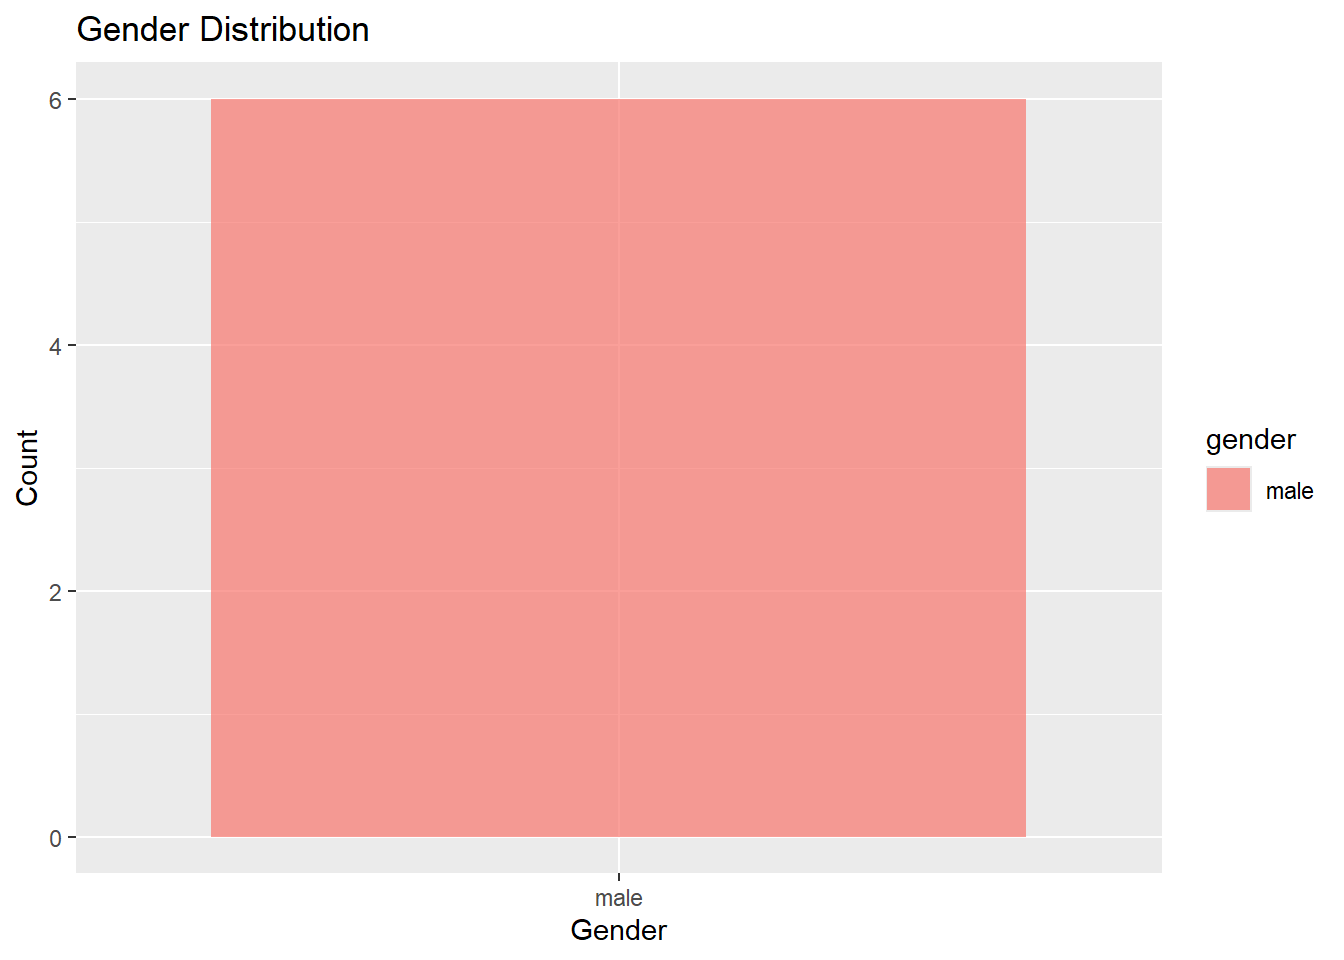
\includegraphics{Survey-Data-Analysis-of-Farmers-in-Jalgaon-District_files/figure-latex/unnamed-chunk-9-1.pdf}

\subsubsection{5.2 Gender Distribution}\label{gender-distribution}

\begin{Shaded}
\begin{Highlighting}[]
\NormalTok{survey\_main }\SpecialCharTok{\%\textgreater{}\%}
  \FunctionTok{count}\NormalTok{(gender) }\SpecialCharTok{\%\textgreater{}\%}
  \FunctionTok{ggplot}\NormalTok{(}\FunctionTok{aes}\NormalTok{(}\AttributeTok{x =}\NormalTok{ gender, }\AttributeTok{y =}\NormalTok{ n, }\AttributeTok{fill =}\NormalTok{ gender)) }\SpecialCharTok{+} 
  \FunctionTok{geom\_bar}\NormalTok{(}\AttributeTok{stat =} \StringTok{"identity"}\NormalTok{, }\AttributeTok{alpha =} \FloatTok{0.7}\NormalTok{) }\SpecialCharTok{+}
  \FunctionTok{labs}\NormalTok{(}\AttributeTok{title =} \StringTok{"Gender Distribution"}\NormalTok{, }\AttributeTok{x =} \StringTok{"Gender"}\NormalTok{, }\AttributeTok{y =} \StringTok{"Count"}\NormalTok{) }\SpecialCharTok{+}
  \FunctionTok{theme\_minimal}\NormalTok{()}
\end{Highlighting}
\end{Shaded}

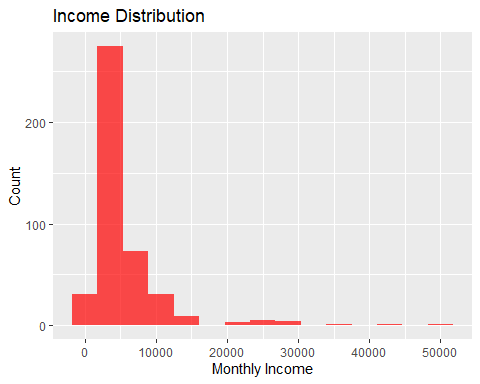
\includegraphics{Survey-Data-Analysis-of-Farmers-in-Jalgaon-District_files/figure-latex/unnamed-chunk-10-1.pdf}

\subsubsection{5.3 Education Levels}\label{education-levels}

\begin{Shaded}
\begin{Highlighting}[]
\NormalTok{survey\_main }\SpecialCharTok{\%\textgreater{}\%}
  \FunctionTok{count}\NormalTok{(education) }\SpecialCharTok{\%\textgreater{}\%}
  \FunctionTok{ggplot}\NormalTok{(}\FunctionTok{aes}\NormalTok{(}\AttributeTok{x =} \FunctionTok{reorder}\NormalTok{(education, n), }\AttributeTok{y =}\NormalTok{ n, }\AttributeTok{fill =}\NormalTok{ education)) }\SpecialCharTok{+}
  \FunctionTok{geom\_bar}\NormalTok{(}\AttributeTok{stat =} \StringTok{"identity"}\NormalTok{) }\SpecialCharTok{+}
  \FunctionTok{coord\_flip}\NormalTok{() }\SpecialCharTok{+}
  \FunctionTok{labs}\NormalTok{(}\AttributeTok{title =} \StringTok{"Education Levels of Farmers"}\NormalTok{, }\AttributeTok{x =} \StringTok{"Education"}\NormalTok{, }\AttributeTok{y =} \StringTok{"Count"}\NormalTok{) }\SpecialCharTok{+}
  \FunctionTok{theme\_minimal}\NormalTok{()}
\end{Highlighting}
\end{Shaded}

\includegraphics{Survey-Data-Analysis-of-Farmers-in-Jalgaon-District_files/figure-latex/unnamed-chunk-11-1.pdf}

\subsubsection{5.4 Income Analysis}\label{income-analysis}

\begin{Shaded}
\begin{Highlighting}[]
\NormalTok{survey\_main }\SpecialCharTok{\%\textgreater{}\%}
  \FunctionTok{ggplot}\NormalTok{(}\FunctionTok{aes}\NormalTok{(}\AttributeTok{x =}\NormalTok{ annual\_income)) }\SpecialCharTok{+} 
  \FunctionTok{geom\_bar}\NormalTok{(}\AttributeTok{fill =} \StringTok{"red"}\NormalTok{, }\AttributeTok{alpha =} \FloatTok{0.7}\NormalTok{) }\SpecialCharTok{+}
  \FunctionTok{labs}\NormalTok{(}\AttributeTok{title =} \StringTok{"Annual Income Distribution"}\NormalTok{, }\AttributeTok{x =} \StringTok{"Income Bracket"}\NormalTok{, }\AttributeTok{y =} \StringTok{"Count"}\NormalTok{) }\SpecialCharTok{+}
  \FunctionTok{theme\_minimal}\NormalTok{() }\SpecialCharTok{+}
  \FunctionTok{theme}\NormalTok{(}\AttributeTok{axis.text.x =} \FunctionTok{element\_text}\NormalTok{(}\AttributeTok{angle =} \DecValTok{45}\NormalTok{, }\AttributeTok{hjust =} \DecValTok{1}\NormalTok{))}
\end{Highlighting}
\end{Shaded}

\includegraphics{Survey-Data-Analysis-of-Farmers-in-Jalgaon-District_files/figure-latex/unnamed-chunk-12-1.pdf}

\subsection{6. Land Ownership and
Agriculture}\label{land-ownership-and-agriculture}

\subsubsection{6.1 Total Land
Distribution}\label{total-land-distribution}

\begin{Shaded}
\begin{Highlighting}[]
\FunctionTok{unique}\NormalTok{(survey\_main}\SpecialCharTok{$}\NormalTok{total\_land)}
\end{Highlighting}
\end{Shaded}

\begin{verbatim}
##  [1] "0"             "02"            "1"             "-"            
##  [5] "3:1/2"         "२"             "००"            "४.०"          
##  [9] "५  १/२"        "७"             "५"             "4"            
## [13] "२५"            "३"             "०५"            "३.१०"         
## [17] "00"            "3"             "3hectr"        "२.५ एकर"      
## [21] "2hec"          "3एकर"          "1.5 एकर"       "4.5"          
## [25] "4एकर"          "8"             "3.5"           "1.75 एकर"     
## [29] "1.57"          "2.75"          "2"             "५ एकर"        
## [33] "10.50 बिघे"     "2.5"           "2 बिघे"         "2.5 बिघे"      
## [37] "5"             "6"             "10 बिघे"        "1.5"          
## [41] "7 बिघे"         "3.2"           "10"            "7"            
## [45] "03"            "1.9"           "1/2"           "01"           
## [49] "17.7"          "2.30.00"       "1.85.00"       "4.5 बिघे"      
## [53] "शेती नाही"      "1.63"          "s"             "3.26"         
## [57] "3.22"          "8.15"          "२.४५"          "11.41"        
## [61] "4.83"          "4.83 बिघे"      "८ .०५ बिगें"     "7.2"          
## [65] "1 एकर"         "4.8"           "1.61 बिघे"      "3.2 बिघे"      
## [69] "8 बि घे"        "3 बिधे"         "12"            "4 बि घे"       
## [73] "5 बि घे"        "१"             "20"            "5 एकर"        
## [77] "6.44"          "2.41"          "सव्वा दोन बिघे"  "08"           
## [81] "1 बिघे"         "18"            "04"            "नाही"         
## [85] "2 हेक्टर"        "दोन हेक्टर 22 R" "12 एकर"        "1.49R"        
## [89] "4 एकर"         "54R"           "2 एकर"         "अर्धा एकर"     
## [93] "7 एकर"         "8.5"           "2.81"          "1 हेक्टर"       
## [97] "1.20 हेक्टर"     "0.6"           "1.7 हेक्टर"
\end{verbatim}

\section{Variable `total\_land' should be numeric. Only then run
following
code}\label{variable-total_land-should-be-numeric.-only-then-run-following-code}

\begin{Shaded}
\begin{Highlighting}[]
\CommentTok{\#survey\_main \%\textgreater{}\%}
\CommentTok{\#  ggplot(aes(x = total\_land)) + }
\CommentTok{\#  geom\_histogram(bins = 15, fill = "green", alpha = 0.7) +}
\CommentTok{\#  labs(title = "Distribution of Total Land Owned", x = "Total Land (bigha/acre)", y = "Count") +}
\CommentTok{\#  theme\_minimal()}
\end{Highlighting}
\end{Shaded}

\subsubsection{6.2 Crops Grown}\label{crops-grown}

\begin{Shaded}
\begin{Highlighting}[]
\NormalTok{survey\_main }\SpecialCharTok{\%\textgreater{}\%}
  \FunctionTok{select}\NormalTok{(cotton, maize, jowar, bajra, pulses, soybean, wheat, gram) }\SpecialCharTok{\%\textgreater{}\%}
  \FunctionTok{summarise\_all}\NormalTok{(mean, }\AttributeTok{na.rm =} \ConstantTok{TRUE}\NormalTok{) }\SpecialCharTok{\%\textgreater{}\%}
  \FunctionTok{pivot\_longer}\NormalTok{(}\FunctionTok{everything}\NormalTok{(), }\AttributeTok{names\_to =} \StringTok{"Crop"}\NormalTok{, }\AttributeTok{values\_to =} \StringTok{"Proportion"}\NormalTok{) }\SpecialCharTok{\%\textgreater{}\%}
  \FunctionTok{ggplot}\NormalTok{(}\FunctionTok{aes}\NormalTok{(}\AttributeTok{x =}\NormalTok{ Crop, }\AttributeTok{y =}\NormalTok{ Proportion, }\AttributeTok{fill =}\NormalTok{ Crop)) }\SpecialCharTok{+}
  \FunctionTok{geom\_bar}\NormalTok{(}\AttributeTok{stat =} \StringTok{"identity"}\NormalTok{) }\SpecialCharTok{+}
  \FunctionTok{labs}\NormalTok{(}\AttributeTok{title =} \StringTok{"Proportion of Farmers Growing Each Crop"}\NormalTok{, }\AttributeTok{y =} \StringTok{"Proportion"}\NormalTok{) }\SpecialCharTok{+}
  \FunctionTok{theme\_minimal}\NormalTok{()}
\end{Highlighting}
\end{Shaded}

\includegraphics{Survey-Data-Analysis-of-Farmers-in-Jalgaon-District_files/figure-latex/unnamed-chunk-15-1.pdf}

\subsection{7. Loan and Financial
Stress}\label{loan-and-financial-stress}

\subsubsection{7.1 Loan Status}\label{loan-status}

\begin{Shaded}
\begin{Highlighting}[]
\NormalTok{survey\_main }\SpecialCharTok{\%\textgreater{}\%}
  \FunctionTok{count}\NormalTok{(loan\_status) }\SpecialCharTok{\%\textgreater{}\%}
  \FunctionTok{ggplot}\NormalTok{(}\FunctionTok{aes}\NormalTok{(}\AttributeTok{x =}\NormalTok{ loan\_status, }\AttributeTok{y =}\NormalTok{ n, }\AttributeTok{fill =}\NormalTok{ loan\_status)) }\SpecialCharTok{+}
  \FunctionTok{geom\_bar}\NormalTok{(}\AttributeTok{stat =} \StringTok{"identity"}\NormalTok{) }\SpecialCharTok{+}
  \FunctionTok{labs}\NormalTok{(}\AttributeTok{title =} \StringTok{"Loan Status Distribution"}\NormalTok{, }\AttributeTok{x =} \StringTok{"Loan Status"}\NormalTok{, }\AttributeTok{y =} \StringTok{"Count"}\NormalTok{) }\SpecialCharTok{+}
  \FunctionTok{theme\_minimal}\NormalTok{()}
\end{Highlighting}
\end{Shaded}

\includegraphics{Survey-Data-Analysis-of-Farmers-in-Jalgaon-District_files/figure-latex/unnamed-chunk-16-1.pdf}

\subsubsection{7.2 Loan Amount vs.~Income}\label{loan-amount-vs.-income}

\begin{Shaded}
\begin{Highlighting}[]
\NormalTok{survey\_main }\SpecialCharTok{\%\textgreater{}\%}
  \FunctionTok{ggplot}\NormalTok{(}\FunctionTok{aes}\NormalTok{(}\AttributeTok{x =}\NormalTok{ annual\_income, }\AttributeTok{y =}\NormalTok{ loan\_amount, }\AttributeTok{fill =}\NormalTok{ annual\_income)) }\SpecialCharTok{+}
  \FunctionTok{geom\_boxplot}\NormalTok{() }\SpecialCharTok{+}
  \FunctionTok{labs}\NormalTok{(}\AttributeTok{title =} \StringTok{"Loan Amount by Annual Income"}\NormalTok{, }\AttributeTok{x =} \StringTok{"Income"}\NormalTok{, }\AttributeTok{y =} \StringTok{"Loan Amount (INR)"}\NormalTok{) }\SpecialCharTok{+}
  \FunctionTok{theme\_minimal}\NormalTok{() }\SpecialCharTok{+}
  \FunctionTok{theme}\NormalTok{(}\AttributeTok{axis.text.x =} \FunctionTok{element\_text}\NormalTok{(}\AttributeTok{angle =} \DecValTok{45}\NormalTok{, }\AttributeTok{hjust =} \DecValTok{1}\NormalTok{))}
\end{Highlighting}
\end{Shaded}

\includegraphics{Survey-Data-Analysis-of-Farmers-in-Jalgaon-District_files/figure-latex/unnamed-chunk-17-1.pdf}

\subsection{8. Mental Health Analysis}\label{mental-health-analysis}

\subsubsection{8.1 Depression Scores}\label{depression-scores}

\begin{Shaded}
\begin{Highlighting}[]
\NormalTok{survey\_main}\SpecialCharTok{$}\NormalTok{depression\_1}
\end{Highlighting}
\end{Shaded}

\begin{verbatim}
##   [1] "often"  "always" "always" "always" "rarely" "rarely" "rarely" "rarely"
##   [9] "always" "always" "rarely" "always" "often"  "often"  "often"  "often" 
##  [17] "often"  "often"  "always" "always" "always" "often"  "often"  "often" 
##  [25] "always" "often"  "rarely" "rarely" "rarely" "always" "always" "always"
##  [33] "rarely" "always" "rarely" "always" "always" "always" "never"  "always"
##  [41] "rarely" "always" "always" "rarely" "often"  "always" "rarely" "often" 
##  [49] "often"  "rarely" "often"  "rarely" "often"  "often"  "often"  "often" 
##  [57] "often"  "rarely" "often"  "often"  "often"  "rarely" "always" "always"
##  [65] "often"  "rarely" "often"  "rarely" "often"  "often"  "always" "often" 
##  [73] "often"  "often"  "always" "often"  "never"  "always" "always" "always"
##  [81] "often"  "often"  "often"  "rarely" "often"  "often"  "often"  "often" 
##  [89] "often"  "always" "rarely" "always" "rarely" "always" "often"  "always"
##  [97] "always" "rarely" "often"  "often"  "rarely" "often"  "rarely" "rarely"
## [105] "never"  "rarely" "rarely" "often"  "always" "often"  "often"  "always"
## [113] "often"  "often"  "always" "always" "always" "often"  "always" "always"
## [121] "rarely" "always" "always" "always" "always" "often"  "often"  "often" 
## [129] "often"  "rarely" "often"  "never"  "often"  "rarely" "often"  "often" 
## [137] "often"  "always" "often"  "rarely" "never"  "rarely" "often"  "rarely"
## [145] "rarely" "often"  "rarely" "rarely" "rarely" "never"  "often"  "always"
## [153] "never"  "rarely" "always" "often"  "often"  "rarely" "always" "never" 
## [161] "rarely" "often"  "rarely" "never"  "often"  "never"  "rarely" "often" 
## [169] "rarely" "rarely" "always" "never"  "always" "rarely" "often"  "often" 
## [177] "never"  "rarely" "rarely" "often"  "never"  "rarely" "rarely" "often" 
## [185] "rarely" "never"  "always" "always" "always" "often"  "always" "always"
## [193] "often"  "often"  "rarely" "never"  "always" "rarely" "rarely" "rarely"
## [201] "always" "rarely" "rarely" "often"  "rarely" "often"  "always" "never" 
## [209] "rarely" "always" "rarely" "rarely" "often"  "rarely" "always" "always"
## [217] "always" "always" "rarely" "rarely" "always" "always" "always" "always"
## [225] "rarely" "rarely" "rarely" "always" "rarely" "always" "never"  "always"
## [233] "rarely" "always" "always" "always" "often"  "often"  "always" "often" 
## [241] "always" "often"  "often"  "always" "rarely" "often"  "always" "often" 
## [249] "often"  "often"  "often"  "often"  "often"  "always" "often"  "always"
## [257] "often"  "rarely" "often"  "often"  "never"  "rarely" "rarely" "rarely"
## [265] "rarely" "often"  "often"  "rarely" "rarely" "rarely" "rarely" "rarely"
## [273] "rarely" "always" "rarely" "always" "never"  "never"  "never"  "never" 
## [281] "rarely" "rarely" "rarely" "rarely" "often"  "often"  "never"  "rarely"
## [289] "often"  "rarely" "often"  "often"  "never"  "rarely" "rarely" "rarely"
## [297] "rarely" "never"  "rarely" "never"  "rarely" "never"  "often"
\end{verbatim}

\begin{Shaded}
\begin{Highlighting}[]
\NormalTok{survey\_main }\SpecialCharTok{\%\textgreater{}\%}
  \FunctionTok{select}\NormalTok{(}\FunctionTok{starts\_with}\NormalTok{(}\StringTok{"depression\_"}\NormalTok{)) }\SpecialCharTok{\%\textgreater{}\%}
  \FunctionTok{pivot\_longer}\NormalTok{(}\FunctionTok{everything}\NormalTok{(), }\AttributeTok{names\_to =} \StringTok{"Question"}\NormalTok{, }\AttributeTok{values\_to =} \StringTok{"Response"}\NormalTok{) }\SpecialCharTok{\%\textgreater{}\%}
  \FunctionTok{count}\NormalTok{(Question, Response) }\SpecialCharTok{\%\textgreater{}\%}
  \FunctionTok{ggplot}\NormalTok{(}\FunctionTok{aes}\NormalTok{(}\AttributeTok{x =}\NormalTok{ Question, }\AttributeTok{y =}\NormalTok{ n, }\AttributeTok{fill =}\NormalTok{ Response)) }\SpecialCharTok{+}
  \FunctionTok{geom\_bar}\NormalTok{(}\AttributeTok{stat =} \StringTok{"identity"}\NormalTok{, }\AttributeTok{position =} \StringTok{"dodge"}\NormalTok{) }\SpecialCharTok{+}
  \FunctionTok{labs}\NormalTok{(}\AttributeTok{title =} \StringTok{"Frequency of Depression Responses"}\NormalTok{, }\AttributeTok{y =} \StringTok{"Count"}\NormalTok{, }\AttributeTok{fill =} \StringTok{"Response Category"}\NormalTok{) }\SpecialCharTok{+}
  \FunctionTok{theme\_minimal}\NormalTok{() }\SpecialCharTok{+}
  \FunctionTok{theme}\NormalTok{(}\AttributeTok{axis.text.x =} \FunctionTok{element\_text}\NormalTok{(}\AttributeTok{angle =} \DecValTok{45}\NormalTok{, }\AttributeTok{hjust =} \DecValTok{1}\NormalTok{))}
\end{Highlighting}
\end{Shaded}

\includegraphics{Survey-Data-Analysis-of-Farmers-in-Jalgaon-District_files/figure-latex/unnamed-chunk-19-1.pdf}

\subsection{9. Government Scheme
Awareness}\label{government-scheme-awareness}

\begin{Shaded}
\begin{Highlighting}[]
\NormalTok{survey\_main }\SpecialCharTok{\%\textgreater{}\%}
  \FunctionTok{select}\NormalTok{(pm\_kisan, pmfby, kisan\_credit) }\SpecialCharTok{\%\textgreater{}\%}
  \FunctionTok{summarise\_all}\NormalTok{(}\SpecialCharTok{\textasciitilde{}}\FunctionTok{sum}\NormalTok{(. }\SpecialCharTok{==} \StringTok{"received\_benefit"}\NormalTok{, }\AttributeTok{na.rm =} \ConstantTok{TRUE}\NormalTok{)) }\SpecialCharTok{\%\textgreater{}\%}
  \FunctionTok{pivot\_longer}\NormalTok{(}\FunctionTok{everything}\NormalTok{(), }\AttributeTok{names\_to =} \StringTok{"Scheme"}\NormalTok{, }\AttributeTok{values\_to =} \StringTok{"Beneficiaries"}\NormalTok{) }\SpecialCharTok{\%\textgreater{}\%}
  \FunctionTok{ggplot}\NormalTok{(}\FunctionTok{aes}\NormalTok{(}\AttributeTok{x =}\NormalTok{ Scheme, }\AttributeTok{y =}\NormalTok{ Beneficiaries, }\AttributeTok{fill =}\NormalTok{ Scheme)) }\SpecialCharTok{+}
  \FunctionTok{geom\_bar}\NormalTok{(}\AttributeTok{stat =} \StringTok{"identity"}\NormalTok{) }\SpecialCharTok{+}
  \FunctionTok{labs}\NormalTok{(}\AttributeTok{title =} \StringTok{"Number of Beneficiaries by Scheme"}\NormalTok{, }\AttributeTok{y =} \StringTok{"Count"}\NormalTok{) }\SpecialCharTok{+}
  \FunctionTok{theme\_minimal}\NormalTok{()}
\end{Highlighting}
\end{Shaded}

\includegraphics{Survey-Data-Analysis-of-Farmers-in-Jalgaon-District_files/figure-latex/unnamed-chunk-20-1.pdf}

\begin{Shaded}
\begin{Highlighting}[]
\NormalTok{generate\_freq\_tables }\OtherTok{\textless{}{-}} \ControlFlowTok{function}\NormalTok{(df, sheet\_name) \{}
  \FunctionTok{cat}\NormalTok{(}\StringTok{"\#\# Frequency Distributions for"}\NormalTok{, sheet\_name, }\StringTok{"}\SpecialCharTok{\textbackslash{}n\textbackslash{}n}\StringTok{"}\NormalTok{)}
  \ControlFlowTok{for}\NormalTok{ (var }\ControlFlowTok{in} \FunctionTok{names}\NormalTok{(df)) \{}
    \FunctionTok{cat}\NormalTok{(}\StringTok{"\#\#\#"}\NormalTok{, var, }\StringTok{"}\SpecialCharTok{\textbackslash{}n}\StringTok{"}\NormalTok{)}
    
    \CommentTok{\# Skip if variable is entirely NA}
    \ControlFlowTok{if}\NormalTok{ (}\FunctionTok{all}\NormalTok{(}\FunctionTok{is.na}\NormalTok{(df[[var]]))) \{}
      \FunctionTok{cat}\NormalTok{(}\StringTok{"Variable"}\NormalTok{, var, }\StringTok{"contains only NA values and is skipped.}\SpecialCharTok{\textbackslash{}n}\StringTok{"}\NormalTok{)}
      \ControlFlowTok{next}
\NormalTok{    \}}
    
    \CommentTok{\# Number of unique non{-}NA values}
\NormalTok{    unique\_vals }\OtherTok{\textless{}{-}} \FunctionTok{length}\NormalTok{(}\FunctionTok{unique}\NormalTok{(}\FunctionTok{na.omit}\NormalTok{(df[[var]])))}
    
    \ControlFlowTok{if}\NormalTok{ (}\FunctionTok{is.factor}\NormalTok{(df[[var]]) }\SpecialCharTok{||} \FunctionTok{is.character}\NormalTok{(df[[var]]) }\SpecialCharTok{||}\NormalTok{ unique\_vals }\SpecialCharTok{\textless{}} \DecValTok{10}\NormalTok{) \{}
      \CommentTok{\# Treat as categorical}
\NormalTok{      freq\_table }\OtherTok{\textless{}{-}} \FunctionTok{table}\NormalTok{(df[[var]], }\AttributeTok{useNA =} \StringTok{"ifany"}\NormalTok{)}
\NormalTok{      prop\_table }\OtherTok{\textless{}{-}} \FunctionTok{prop.table}\NormalTok{(freq\_table) }\SpecialCharTok{*} \DecValTok{100}
\NormalTok{      combined\_table }\OtherTok{\textless{}{-}} \FunctionTok{cbind}\NormalTok{(}\AttributeTok{Count =}\NormalTok{ freq\_table, }\AttributeTok{Percentage =} \FunctionTok{round}\NormalTok{(prop\_table, }\DecValTok{2}\NormalTok{))}
      \FunctionTok{print}\NormalTok{(}\FunctionTok{kable}\NormalTok{(combined\_table, }\AttributeTok{caption =} \FunctionTok{paste}\NormalTok{(}\StringTok{"Frequency table for"}\NormalTok{, var)))}
\NormalTok{    \} }\ControlFlowTok{else} \ControlFlowTok{if}\NormalTok{ (}\FunctionTok{is.numeric}\NormalTok{(df[[var]]) }\SpecialCharTok{\&\&}\NormalTok{ unique\_vals }\SpecialCharTok{\textgreater{}=} \DecValTok{10}\NormalTok{) \{}
      \CommentTok{\# Treat as continuous and attempt binning}
\NormalTok{      breaks }\OtherTok{\textless{}{-}} \FunctionTok{quantile}\NormalTok{(df[[var]], }\AttributeTok{probs =} \FunctionTok{seq}\NormalTok{(}\DecValTok{0}\NormalTok{, }\DecValTok{1}\NormalTok{, }\AttributeTok{by =} \FloatTok{0.2}\NormalTok{), }\AttributeTok{na.rm =} \ConstantTok{TRUE}\NormalTok{)}
      \ControlFlowTok{if}\NormalTok{ (}\FunctionTok{length}\NormalTok{(}\FunctionTok{unique}\NormalTok{(breaks)) }\SpecialCharTok{\textless{}} \FunctionTok{length}\NormalTok{(breaks)) \{}
        \FunctionTok{cat}\NormalTok{(}\StringTok{"Note: Variable"}\NormalTok{, var, }\StringTok{"has duplicate breaks and will be treated as categorical.}\SpecialCharTok{\textbackslash{}n}\StringTok{"}\NormalTok{)}
\NormalTok{        freq\_table }\OtherTok{\textless{}{-}} \FunctionTok{table}\NormalTok{(df[[var]], }\AttributeTok{useNA =} \StringTok{"ifany"}\NormalTok{)}
\NormalTok{        prop\_table }\OtherTok{\textless{}{-}} \FunctionTok{prop.table}\NormalTok{(freq\_table) }\SpecialCharTok{*} \DecValTok{100}
\NormalTok{        combined\_table }\OtherTok{\textless{}{-}} \FunctionTok{cbind}\NormalTok{(}\AttributeTok{Count =}\NormalTok{ freq\_table, }\AttributeTok{Percentage =} \FunctionTok{round}\NormalTok{(prop\_table, }\DecValTok{2}\NormalTok{))}
        \FunctionTok{print}\NormalTok{(}\FunctionTok{kable}\NormalTok{(combined\_table, }\AttributeTok{caption =} \FunctionTok{paste}\NormalTok{(}\StringTok{"Frequency table for"}\NormalTok{, var, }\StringTok{"(categorical due to duplicate breaks)"}\NormalTok{)))}
\NormalTok{      \} }\ControlFlowTok{else}\NormalTok{ \{}
        \CommentTok{\# Proceed with binning}
\NormalTok{        binned }\OtherTok{\textless{}{-}} \FunctionTok{cut}\NormalTok{(df[[var]], }\AttributeTok{breaks =}\NormalTok{ breaks, }\AttributeTok{include.lowest =} \ConstantTok{TRUE}\NormalTok{, }\AttributeTok{dig.lab =} \DecValTok{5}\NormalTok{)}
\NormalTok{        freq\_table }\OtherTok{\textless{}{-}} \FunctionTok{table}\NormalTok{(binned, }\AttributeTok{useNA =} \StringTok{"ifany"}\NormalTok{)}
\NormalTok{        prop\_table }\OtherTok{\textless{}{-}} \FunctionTok{prop.table}\NormalTok{(freq\_table) }\SpecialCharTok{*} \DecValTok{100}
\NormalTok{        combined\_table }\OtherTok{\textless{}{-}} \FunctionTok{cbind}\NormalTok{(}\AttributeTok{Count =}\NormalTok{ freq\_table, }\AttributeTok{Percentage =} \FunctionTok{round}\NormalTok{(prop\_table, }\DecValTok{2}\NormalTok{))}
        \FunctionTok{print}\NormalTok{(}\FunctionTok{kable}\NormalTok{(combined\_table, }\AttributeTok{caption =} \FunctionTok{paste}\NormalTok{(}\StringTok{"Frequency table for"}\NormalTok{, var, }\StringTok{"(binned)"}\NormalTok{)))}
\NormalTok{      \}}
\NormalTok{    \} }\ControlFlowTok{else}\NormalTok{ \{}
      \FunctionTok{cat}\NormalTok{(}\StringTok{"Variable"}\NormalTok{, var, }\StringTok{"is of type"}\NormalTok{, }\FunctionTok{class}\NormalTok{(df[[var]]), }\StringTok{"and will be skipped.}\SpecialCharTok{\textbackslash{}n}\StringTok{"}\NormalTok{)}
\NormalTok{    \}}
    \FunctionTok{cat}\NormalTok{(}\StringTok{"}\SpecialCharTok{\textbackslash{}n\textbackslash{}n}\StringTok{"}\NormalTok{)}
\NormalTok{  \}}
\NormalTok{\}}
\end{Highlighting}
\end{Shaded}

\begin{Shaded}
\begin{Highlighting}[]
\FunctionTok{generate\_freq\_tables}\NormalTok{(survey\_main, }\StringTok{"Main Survey Data"}\NormalTok{)}
\end{Highlighting}
\end{Shaded}

\begin{verbatim}
## ## Frequency Distributions for Main Survey Data 
## 
## ### farmer_id 
## 
## 
## Table: Frequency table for farmer_id
## 
## |           | Count| Percentage|
## |:----------|-----:|----------:|
## |001-2022   |     1|       0.33|
## |002-2022   |     1|       0.33|
## |003-2022   |     1|       0.33|
## |006-2022   |     1|       0.33|
## |008-2022   |     1|       0.33|
## |015-2022   |     1|       0.33|
## |017-2022   |     1|       0.33|
## |018-2022   |     1|       0.33|
## |019-2022   |     1|       0.33|
## |021-2022   |     1|       0.33|
## |025-2022   |     1|       0.33|
## |027-2022   |     1|       0.33|
## |028-2022   |     1|       0.33|
## |034-2022   |     1|       0.33|
## |037-2022   |     1|       0.33|
## |039-2022   |     1|       0.33|
## |041-2022   |     1|       0.33|
## |042-2022   |     1|       0.33|
## |051-2022   |     1|       0.33|
## |056-2022   |     1|       0.33|
## |062-2022   |     1|       0.33|
## |063-2022   |     1|       0.33|
## |065-2022   |     1|       0.33|
## |073-2022   |     1|       0.33|
## |075-2022   |     1|       0.33|
## |081-2022   |     1|       0.33|
## |082-2022   |     1|       0.33|
## |084-2022   |     1|       0.33|
## |091-2022   |     1|       0.33|
## |097-2022   |     1|       0.33|
## |०९८-२०२२   |     1|       0.33|
## |10-2022    |     1|       0.33|
## |101-2022   |     1|       0.33|
## |102-2022   |     1|       0.33|
## |104-2022   |     1|       0.33|
## |105-2022   |     1|       0.33|
## |108        |     1|       0.33|
## |109 -2022  |     1|       0.33|
## |110-2022   |     1|       0.33|
## |111-2022   |     1|       0.33|
## |112-2022   |     1|       0.33|
## |113-2022   |     1|       0.33|
## |114        |     1|       0.33|
## |115-2022   |     1|       0.33|
## |116-2022   |     1|       0.33|
## |118 -2025  |     1|       0.33|
## |119-2022   |     1|       0.33|
## |12-2022    |     1|       0.33|
## |120-2022   |     1|       0.33|
## |121-2022   |     1|       0.33|
## |122-2022   |     1|       0.33|
## |123        |     1|       0.33|
## |124-2022   |     1|       0.33|
## |125-2022   |     1|       0.33|
## |126-2022   |     1|       0.33|
## |127-2022   |     1|       0.33|
## |128-2023   |     1|       0.33|
## |129-2023   |     1|       0.33|
## |13-2022    |     1|       0.33|
## |130        |     1|       0.33|
## |131-2023   |     1|       0.33|
## |132-2023   |     1|       0.33|
## |133-2023   |     1|       0.33|
## |134-2023   |     1|       0.33|
## |135-2023   |     1|       0.33|
## |137-2023   |     1|       0.33|
## |138-2023   |     1|       0.33|
## |139-2023   |     1|       0.33|
## |14-2022    |     1|       0.33|
## |140-2023   |     1|       0.33|
## |141-2023   |     1|       0.33|
## |142-2023   |     1|       0.33|
## |144-2023   |     1|       0.33|
## |१४५-२०२३   |     1|       0.33|
## |146-2023   |     1|       0.33|
## |147-2023   |     1|       0.33|
## |148-2023   |     1|       0.33|
## |149-2023   |     1|       0.33|
## |150-2023   |     1|       0.33|
## |152-2023   |     1|       0.33|
## |153- 2023  |     1|       0.33|
## |154-2023   |     1|       0.33|
## |155- 2023  |     1|       0.33|
## |157-2023   |     1|       0.33|
## |158-2023   |     1|       0.33|
## |159-2023   |     1|       0.33|
## |16-2022    |     1|       0.33|
## |160- 2025  |     1|       0.33|
## |161- 2025  |     1|       0.33|
## |163-2023   |     1|       0.33|
## |164-2023   |     1|       0.33|
## |165-2023   |     1|       0.33|
## |166-2023   |     1|       0.33|
## |167-2023   |     1|       0.33|
## |168-2023   |     1|       0.33|
## |169-2023   |     1|       0.33|
## |170-2023   |     1|       0.33|
## |171- 2023  |     1|       0.33|
## |172-2023   |     1|       0.33|
## |173-2023   |     1|       0.33|
## |174-2023   |     1|       0.33|
## |175-2023   |     1|       0.33|
## |177-2023   |     1|       0.33|
## |178-2023   |     1|       0.33|
## |179-2023   |     1|       0.33|
## |180-2025   |     1|       0.33|
## |181-2023   |     1|       0.33|
## |182-2023   |     1|       0.33|
## |183-2023   |     1|       0.33|
## |184-2023   |     1|       0.33|
## |186-2023   |     1|       0.33|
## |187-2023   |     1|       0.33|
## |190-2023   |     1|       0.33|
## |191-2023   |     1|       0.33|
## |१९३-२०२३   |     1|       0.33|
## |195-2023   |     1|       0.33|
## |196-2023   |     1|       0.33|
## |198-2023   |     1|       0.33|
## |199-2023   |     1|       0.33|
## |20-2022    |     1|       0.33|
## |200-2023   |     1|       0.33|
## |201-2023   |     1|       0.33|
## |202-2023   |     1|       0.33|
## |203-2023   |     1|       0.33|
## |204-2023   |     1|       0.33|
## |205-2023   |     1|       0.33|
## |206-2023   |     1|       0.33|
## |207-2023   |     1|       0.33|
## |208-2023   |     1|       0.33|
## |209-2023   |     1|       0.33|
## |211-2023   |     1|       0.33|
## |212-2023   |     1|       0.33|
## |213-2023   |     1|       0.33|
## |214-2023   |     1|       0.33|
## |215-2023   |     1|       0.33|
## |216-2023   |     1|       0.33|
## |217-2023   |     1|       0.33|
## |218-2023   |     1|       0.33|
## |219-2023   |     1|       0.33|
## |220-2023   |     1|       0.33|
## |२२२-२०२३   |     1|       0.33|
## |223-2023   |     1|       0.33|
## |224-2023   |     1|       0.33|
## |226-2023   |     1|       0.33|
## |227-2023   |     1|       0.33|
## |229-2024   |     1|       0.33|
## |230- 2025  |     1|       0.33|
## |231-2024   |     1|       0.33|
## |232-2024   |     1|       0.33|
## |233-2024   |     1|       0.33|
## |234-2024   |     1|       0.33|
## |235-2024   |     1|       0.33|
## |236-2024   |     1|       0.33|
## |237-2024   |     1|       0.33|
## |238-2024   |     1|       0.33|
## |24-2022    |     1|       0.33|
## |240- 2024  |     1|       0.33|
## |241-2024   |     1|       0.33|
## |243-2025   |     1|       0.33|
## |244-2024   |     1|       0.33|
## |245-2024   |     1|       0.33|
## |246-2024   |     1|       0.33|
## |247-2025   |     1|       0.33|
## |248-2024   |     1|       0.33|
## |250- 2024  |     1|       0.33|
## |251-2024   |     1|       0.33|
## |253-2024   |     1|       0.33|
## |254-2024   |     1|       0.33|
## |256-2024   |     1|       0.33|
## |257-2024   |     1|       0.33|
## |258-2024   |     1|       0.33|
## |259-2024   |     1|       0.33|
## |260-2024   |     1|       0.33|
## |261-2024   |     1|       0.33|
## |262-2024   |     1|       0.33|
## |263-2024   |     1|       0.33|
## |264 - 2024 |     1|       0.33|
## |265-2024   |     1|       0.33|
## |267-2024   |     1|       0.33|
## |268-2024   |     1|       0.33|
## |269-2024   |     1|       0.33|
## |272-2024   |     1|       0.33|
## |274- 2025  |     1|       0.33|
## |275 -2025  |     1|       0.33|
## |276- 2024  |     1|       0.33|
## |277-2024   |     1|       0.33|
## |278-2024   |     1|       0.33|
## |280-2024   |     1|       0.33|
## |281-2024   |     1|       0.33|
## |283-2024   |     1|       0.33|
## |284-2024   |     1|       0.33|
## |285-2024   |     1|       0.33|
## |286-2024   |     1|       0.33|
## |287-2024   |     1|       0.33|
## |288-2024   |     1|       0.33|
## |289-2024   |     1|       0.33|
## |29-2022    |     1|       0.33|
## |291-2024   |     1|       0.33|
## |292-2024   |     1|       0.33|
## |293-2024   |     1|       0.33|
## |294-2024   |     1|       0.33|
## |295-2024   |     1|       0.33|
## |296-2024   |     1|       0.33|
## |297-2024   |     1|       0.33|
## |298-2024   |     1|       0.33|
## |299-2024   |     1|       0.33|
## |300-2024   |     1|       0.33|
## |301-2024   |     1|       0.33|
## |305-2024   |     1|       0.33|
## |306        |     1|       0.33|
## |307-2024   |     1|       0.33|
## |308- 2024  |     1|       0.33|
## |31-2022    |     1|       0.33|
## |36-2022    |     1|       0.33|
## |38-2022    |     1|       0.33|
## |4-2022     |     1|       0.33|
## |43-2022    |     1|       0.33|
## |44         |     1|       0.33|
## |45-2022    |     1|       0.33|
## |48-2022    |     1|       0.33|
## |49-2022    |     1|       0.33|
## |5-2022     |     1|       0.33|
## |52-2022    |     1|       0.33|
## |53-2022    |     1|       0.33|
## |54-2022    |     1|       0.33|
## |57--2022   |     1|       0.33|
## |58-2022    |     1|       0.33|
## |59-2022    |     1|       0.33|
## |60-2022    |     1|       0.33|
## |61-2022    |     1|       0.33|
## |66-2022    |     1|       0.33|
## |67-2022    |     1|       0.33|
## |69         |     1|       0.33|
## |7-2022     |     1|       0.33|
## |70-2022    |     1|       0.33|
## |71-2022    |     1|       0.33|
## |74-2022    |     1|       0.33|
## |76-२०२५    |     1|       0.33|
## |77-2022    |     1|       0.33|
## |78-2022    |     1|       0.33|
## |792-2022   |     1|       0.33|
## |85-2022    |     1|       0.33|
## |88- 2025   |     1|       0.33|
## |89-2022    |     1|       0.33|
## |90-2022    |     1|       0.33|
## |92 -2023   |     1|       0.33|
## |94-2022    |     1|       0.33|
## |95-2022    |     1|       0.33|
## |NA         |    55|      18.15|
## 
## 
## ### farmers_name 
## 
## 
## Table: Frequency table for farmers_name
## 
## |                              | Count| Percentage|
## |:-----------------------------|-----:|----------:|
## |Jitendra Raghunath Jadhav     |     1|       0.33|
## |अंकुश सरीचंद naik                |     1|       0.33|
## |अंबादास जनार्दन जवरे             |     1|       0.33|
## |अक्षय अशोक मोरे                 |     1|       0.33|
## |अक्षय समाधान पाटील             |     1|       0.33|
## |अजबसिंग बाबूलाल परदेशी           |     1|       0.33|
## |अतुल देविदास महाजन              |     1|       0.33|
## |अतुल प्रेमसिंग पवार               |     1|       0.33|
## |अनंता रामचंद्र चोपडे              |     1|       0.33|
## |अनिता गजानन कोळी              |     1|       0.33|
## |अनिल दगडू सपकाळे                |     1|       0.33|
## |अनिल शंकर शेळके                  |     1|       0.33|
## |अनिल शामराव पाटील             |     1|       0.33|
## |अनिल श्रीराम पाटील             |     1|       0.33|
## |अनिल साहेबराव पाटील            |     1|       0.33|
## |अमरसिंग मांगो वंजारी             |     1|       0.33|
## |अमोल अरुण पाटील                |     1|       0.33|
## |अमोल संजय लवांडे                 |     1|       0.33|
## |अरुण अमृत धनगर                  |     1|       0.33|
## |अरुण उत्तम लवाडे                 |     1|       0.33|
## |अरुण दगडू भावासार               |     1|       0.33|
## |अरुण रामकृष्ण कोळी               |     1|       0.33|
## |अरुणकुमार प्रताप पाटील           |     1|       0.33|
## |अरुणाबाई शरद पाटील             |     1|       0.33|
## |अर्जुन सुकदेव पाटील               |     1|       0.33|
## |अशोक गजमल पाटील               |     1|       0.33|
## |अशोक बाबुराव बोरसे              |     1|       0.33|
## |आधार एलचंद मोरे                 |     1|       0.33|
## |आनंदा रामदास chaudhari         |     1|       0.33|
## |आनंदा रामभाऊ पाटील             |     1|       0.33|
## |आबा विक्रम पवार                |     1|       0.33|
## |आबा शिवराम निकम               |     1|       0.33|
## |आशाबाई अधिकार पाटील           |     1|       0.33|
## |आसाराम राणू जोशी               |     1|       0.33|
## |ईश्वर विठ्ठल हिरे (सुतार )        |     1|       0.33|
## |उत्तम अमरसिंग नाईक              |     1|       0.33|
## |ऋषिकेश दिलीप खोडपे              |     1|       0.33|
## |एकनाथ रतन पगारे                |     1|       0.33|
## |कपूरचंद महारू पवार               |     1|       0.33|
## |कवरसिंग अमरसिंग पाटील           |     1|       0.33|
## |कविता  विकास कोळी             |     1|       0.33|
## |कांतीलाल गोविंदा पाटील          |     1|       0.33|
## |कांतीलाल नांना पाटील            |     1|       0.33|
## |काशिनाथ पुरषोत्तम कुमावत         |     1|       0.33|
## |किशोर बाळासाहेब पाटील          |     1|       0.33|
## |किसन पंडीत सोनवणे               |     1|       0.33|
## |कै . सविता शरद पाटील           |     1|       0.33|
## |कै. जीवन ज्ञानेश्वर भागवत         |     1|       0.33|
## |कैलास काशिनाथ पाटील            |     1|       0.33|
## |कैलास नामदेव पाटील              |     1|       0.33|
## |कैलास भिवसन पाटील              |     2|       0.66|
## |कैलास रघुनाथ गायकवाड            |     1|       0.33|
## |कैलास वामन गवळी                |     1|       0.33|
## |गजानन  रामदास सोनवणे           |     1|       0.33|
## |गजानन कडू देसाई                 |     1|       0.33|
## |गजानन नारायण महाजन            |     1|       0.33|
## |गजानन मन्साराम  पाटील          |     1|       0.33|
## |गजानन रामचंद्र घुगरे              |     1|       0.33|
## |गणेश ओंकार पाटील                |     1|       0.33|
## |गणेश दगडू पवार                  |     1|       0.33|
## |गणेश नामदेव चौधरी (माळी)        |     1|       0.33|
## |गणेश प्रकाश सैंदाणे                |     1|       0.33|
## |गोंडू रामा कोळी (पिंपळकर)        |     1|       0.33|
## |गोकुळ पांडुरंग वराडे               |     1|       0.33|
## |गोपाल नारायण पाटील / राजपूत    |     1|       0.33|
## |गोपाल शिवाजी गटमने             |     1|       0.33|
## |गोरख ईश्वर महाजन               |     1|       0.33|
## |चंद्रकांत भाऊलाल पाटील           |     1|       0.33|
## |छगन चत्रु राठोड                 |     1|       0.33|
## |छोटू रमण पाटील                 |     1|       0.33|
## |जगन्नाथ किसन पाटील             |     1|       0.33|
## |जिजाबराव संतोष पाटील           |     1|       0.33|
## |जितेंद्र हिरामण कोळी             |     1|       0.33|
## |ज्ञानदेव जयराम सपकाळे            |     1|       0.33|
## |ज्ञानदेव श्रावण मंडलिक            |     1|       0.33|
## |ज्ञानेश्वर अशोक वखरे              |     1|       0.33|
## |ज्ञानेश्वर उर्फ नाना मांगो पाटील   |     1|       0.33|
## |ज्ञानेश्वर एकनाथ पाटील           |     1|       0.33|
## |ज्ञानेश्वर एकनाथ माळी            |     1|       0.33|
## |ज्ञानेश्वर गंगाराम धनगर           |     1|       0.33|
## |ज्ञानेश्वर तुकाराम बारी (खलसे)     |     1|       0.33|
## |ज्ञानेश्वर पुंडलिक पाकळे (धनगर)     |     1|       0.33|
## |ज्ञानेश्वर रामचंद्र पाटील          |     1|       0.33|
## |ज्ञानेश्वर विठ्ठल गायकवाड         |     1|       0.33|
## |ज्ञानेश्वर संजय धनगर              |     1|       0.33|
## |तुकाराम संतोष पाटील             |     1|       0.33|
## |तुकाराम हंसराज वंजारी            |     1|       0.33|
## |तुकाराम हिलाल पाटील            |     1|       0.33|
## |दंगल शिवाजी पाटील              |     1|       0.33|
## |दरबार प्रेमराज चौहान            |     1|       0.33|
## |दशरथ भीमराव तांदळे              |     1|       0.33|
## |दादाराव बाबुराव देशमुख           |     1|       0.33|
## |दिनकर त्रंबक बेलदार              |     1|       0.33|
## |दिनेश रमेश खिरळकर               |     1|       0.33|
## |दिपक बाबूलाल पाटील             |     1|       0.33|
## |दिपक रमेश महाजन                |     1|       0.33|
## |दिपक श्रावण जोहरे               |     1|       0.33|
## |दिलिप कथू पाटील                |     1|       0.33|
## |दिलीप बळीराम पाटील            |     1|       0.33|
## |दिलीप भाईदास मैराळे             |     1|       0.33|
## |दिलीप मुरलीधर पाटील            |     1|       0.33|
## |दिलीप सदा शिरसाठ              |     1|       0.33|
## |दीपक आत्माराम पाटील            |     1|       0.33|
## |दीपक रमण पाटील                |     1|       0.33|
## |दुर्गेश सुभाष दुटे                  |     1|       0.33|
## |देवमन शंकर सोनवणे                |     1|       0.33|
## |देवा एकनाथ धनगर                |     1|       0.33|
## |देविदास मधुकर पाटील             |     1|       0.33|
## |धनंजय सुपडू पाटील                |     1|       0.33|
## |नंदलाल निंबा शिंपी               |     1|       0.33|
## |नंदा ओंकार पवळ                  |     1|       0.33|
## |नरेंद्र भिकन पाटील               |     1|       0.33|
## |नरेंद्र विठ्ठल बलक                |     1|       0.33|
## |नाना पुंडलिक कोळी               |     1|       0.33|
## |नामदेव भगवान कोळी (सेंदाणे )      |     1|       0.33|
## |नामदेव भिला मराठे               |     1|       0.33|
## |नारायण दंगल पाटील              |     2|       0.66|
## |नारायण बाबुराव पाटील           |     1|       0.33|
## |नारायण रामलाल माळी            |     1|       0.33|
## |नितीन कृष्णराव पाटील            |     1|       0.33|
## |पंकज राजेंद्र पाटील               |     1|       0.33|
## |पंडित एकनाथ सपकाळ              |     1|       0.33|
## |परभत रूपा कोळी                 |     1|       0.33|
## |पवन सुभाष पाटील                |     1|       0.33|
## |पाटील भरतकुमार मुरलीधर          |     1|       0.33|
## |पाटील हेमराज शेखर               |     1|       0.33|
## |पापालाल बबन जाधव              |     1|       0.33|
## |प्रकाश  शंकर बारी               |     1|       0.33|
## |प्रकाश किसन पाटील              |     2|       0.66|
## |प्रकाश डिगंबर पाटील             |     1|       0.33|
## |प्रकाश फुलचंद तेली                |     1|       0.33|
## |प्रकाश रमेश माळी                |     1|       0.33|
## |प्रकाश लक्ष्मण पाटील             |     1|       0.33|
## |प्रदिप नामदेव पाटील             |     1|       0.33|
## |प्रदीप देविदास पाटील            |     1|       0.33|
## |प्रदीप नारायण कोल्हे             |     1|       0.33|
## |प्रदीप प्रभाकर तुके               |     1|       0.33|
## |प्रदीप रतन कोळी                |     1|       0.33|
## |प्रवीण धोंडू इंगळे                 |     1|       0.33|
## |प्रशांत वाल्मिक पाटील            |     1|       0.33|
## |प्रेमराज खांडेराव पाटील           |     1|       0.33|
## |प्रेमराज धुळकू कोळी               |     1|       0.33|
## |प्रेमसिंग सोनसिंग पवार            |     1|       0.33|
## |बद्रिसिंग पूना चव्हाण             |     1|       0.33|
## |बळीराम गरमख राठोड             |     1|       0.33|
## |बळीराम नत्थू चव्हाण              |     1|       0.33|
## |बापुराव पुंडलिक कावडे             |     1|       0.33|
## |बापू तुळशीराम कोळी              |     1|       0.33|
## |बापू पुंडलीक महाजन               |     1|       0.33|
## |बापू रामदास गावंडे               |     1|       0.33|
## |बापू सखाराम भिल                |     1|       0.33|
## |बाळासाहेब हिम्मत पाटील          |     1|       0.33|
## |बाळू लहु पाटील                  |     1|       0.33|
## |भगवान पंडित बावस्कर             |     1|       0.33|
## |भगवान भावराव पाटील            |     1|       0.33|
## |भगवान यादव पाटील              |     1|       0.33|
## |भगवान राजमल पाटील             |     1|       0.33|
## |भगवान वसंत पाटील               |     1|       0.33|
## |भगवान वामन धनगर               |     1|       0.33|
## |भगवान विलायचंद कुमावत           |     1|       0.33|
## |भरत तुकाराम धनगर               |     1|       0.33|
## |भरत युवराज पाटील               |     1|       0.33|
## |भाईदास दयाराम कोळी            |     1|       0.33|
## |भागवत प्रल्हाद पाटील            |     1|       0.33|
## |भागवत रघुनाथ पाटील             |     1|       0.33|
## |भागवत रामदास साठे              |     1|       0.33|
## |भालचंद्र किसन पाटील             |     1|       0.33|
## |भावेश भगवान वाघ / मराठे         |     1|       0.33|
## |भूषण रवींद्र पाटील               |     1|       0.33|
## |मंगलसिंग विजयसिंग पाटील          |     1|       0.33|
## |मंगा चिंधू  माळी                 |     1|       0.33|
## |मगन धर्मा चव्हाण                |     1|       0.33|
## |मच्छिंद्र भिवसन पाटील            |     1|       0.33|
## |मधुकर मुरलीधर जगताप             |     1|       0.33|
## |महादू झिपरू पाटील               |     1|       0.33|
## |महारू दशरथ पाटील               |     1|       0.33|
## |महेंद्र दिलीप कोळी (भोलाने)       |     1|       0.33|
## |महेंद्र विनायक सोनवणे             |     1|       0.33|
## |महेंद्र संतोष देवरे                 |     1|       0.33|
## |मुकेश गोपाल माळी                |     1|       0.33|
## |मोहनसिंग इंद्रसिंग पाटील ( सुरडकर) |     1|       0.33|
## |युवराजसिंग नवलसिंग पाटील         |     1|       0.33|
## |योगेश दिलीप पाटील              |     1|       0.33|
## |योगेश रामधन पाटील              |     1|       0.33|
## |रंगनाथ नथू पाटील                |     1|       0.33|
## |रघुनाथ त्र्यंबक कुंभार              |     1|       0.33|
## |रघुनाथ सुका कोळी                |     1|       0.33|
## |रणजीतसिंग पदमसिंग परदेशी         |     1|       0.33|
## |रमेश नामदेव महाजन               |     1|       0.33|
## |रमेश भवराव निकम                |     1|       0.33|
## |रमेश भाईदास जगताप              |     1|       0.33|
## |रमेश विश्राम पाटील              |     1|       0.33|
## |रविंद्र  ओंकार चव्हाण             |     1|       0.33|
## |रविंद्र कौतिक पाटील             |     1|       0.33|
## |रविंद्र यशवंत पाटील              |     1|       0.33|
## |रविंद्र रामदास डहाके (साळुंके)      |     1|       0.33|
## |रवींद्र दशरथ महाजन              |     1|       0.33|
## |रवींद्र बापू महाजन               |     1|       0.33|
## |रवींद्र राजाराम पाटील           |     1|       0.33|
## |राकेश रवींद्र पाटील              |     1|       0.33|
## |राजु सुकलाल माळी                |     1|       0.33|
## |राजू राघो पाटील                |     1|       0.33|
## |राजू सुकलाल मराठे                |     1|       0.33|
## |राजेंद्र गजमल पाटील              |     1|       0.33|
## |राजेंद्र चिंतामण पाटील            |     1|       0.33|
## |राजेंद्र ज्ञानदेव शिंदे              |     1|       0.33|
## |राजेंद्र नाना पाटील              |     1|       0.33|
## |राजेंद्र मधुकर चौधरी              |     1|       0.33|
## |राजेंद्र रमेश महाले                |     1|       0.33|
## |राजेश छोटूलाल पाटील             |     1|       0.33|
## |राजेश सुकलाल कोळी               |     1|       0.33|
## |रामकृष्ण भाईदास पाटील           |     1|       0.33|
## |रावण बोमटू पाटील               |     1|       0.33|
## |राहुल मच्छिंद्र बाविस्कर           |     1|       0.33|
## |रुषीकेश गुलाब पाटील              |     1|       0.33|
## |लक्ष्मण रघुनाथ धनगर              |     1|       0.33|
## |ललित विनायक साळुंखे              |     1|       0.33|
## |ललित संजय झोपे                  |     1|       0.33|
## |लीलाधर रघुनाथ धनगर             |     1|       0.33|
## |वाडीलाल तोताराम पवार          |     1|       0.33|
## |वाल्मिक पोपट पाटील             |     1|       0.33|
## |वाल्मिक वामन पाटील             |     1|       0.33|
## |वासुदेव जगदेव गुरचळ               |     1|       0.33|
## |विकास धनाराज राठोड            |     1|       0.33|
## |विकास भगवान नप्ते               |     1|       0.33|
## |विक्रम लालू भिरुड                |     1|       0.33|
## |विक्रम शिवराम पाटील            |     1|       0.33|
## |विजय भाऊराव पाटील             |     1|       0.33|
## |विजया प्रदीप पाटील             |     1|       0.33|
## |विठोबा गणेश पाटील              |     1|       0.33|
## |विठ्ठल विरभान पाटील            |     1|       0.33|
## |विनोद एकनाथ काकर              |     1|       0.33|
## |विरभान रतन एरंडे                |     1|       0.33|
## |विलास भागवत चोपडे              |     1|       0.33|
## |विलास रामराव पाटील            |     1|       0.33|
## |विश्वनाथ त्रंबक कोळी             |     1|       0.33|
## |शंकर कृष्णा माळी                 |     1|       0.33|
## |शरद खंडू पवार                   |     1|       0.33|
## |शरद जगन्नाथ पाटील              |     1|       0.33|
## |शरद भरत पाटील                 |     1|       0.33|
## |शरद श्रावण पाटील               |     1|       0.33|
## |शशिकांत पृथ्वीराज पाटील          |     1|       0.33|
## |शालिक वामन पाटील              |     1|       0.33|
## |शिवराम तुकाराम कोळी            |     1|       0.33|
## |शिवराम रोडू तेली (परदेशी)        |     1|       0.33|
## |शिवाजी चिंधू पाटील              |     1|       0.33|
## |शिवाजी नथ्थू महाजन              |     1|       0.33|
## |शिवाजी लक्ष्मण चव्हाण            |     1|       0.33|
## |श्रावण लक्ष्मण कोळी              |     1|       0.33|
## |श्रावण सुरेश जाधव                |     1|       0.33|
## |संजय अर्जुन पाटील                |     1|       0.33|
## |संजय जगन्नाथ मानकर              |     1|       0.33|
## |संजय तुकाराम जावळे               |     1|       0.33|
## |संजय दौलत पाटील                |     1|       0.33|
## |संजय भगवान राजपूत               |     1|       0.33|
## |संजय मिठाराम महाजन             |     1|       0.33|
## |संजय सीताराम सोनावणे            |     1|       0.33|
## |संदिप अर्जुन जगताप               |     1|       0.33|
## |संदिप दिगांबर पाटील             |     1|       0.33|
## |संदीप नाना पाटील               |     1|       0.33|
## |संदीप भिला पाटील               |     1|       0.33|
## |संदीप विश्वास पाटील             |     1|       0.33|
## |संदीप संतोष पवार                |     1|       0.33|
## |सखाराम बुधा धनगर               |     1|       0.33|
## |सचिन प्रकाश पाटील              |     2|       0.66|
## |सतीश भागवत पाटील              |     1|       0.33|
## |सतीष चिंतामण पाटील             |     1|       0.33|
## |सतीष मोहन वानखेडे               |     1|       0.33|
## |समाधान एकनाथ धनगर             |     1|       0.33|
## |समाधान भास्कर पाटील            |     1|       0.33|
## |समाधान भीमराव वाघ             |     1|       0.33|
## |समाधान रघुनाथ पाटील            |     1|       0.33|
## |सागर उत्तम गवळी                |     1|       0.33|
## |सागर कृष्णकांत माळी              |     1|       0.33|
## |सागर राजेंद्र सोमवंशी             |     1|       0.33|
## |साहेबराव भाऊराव पाटील          |     1|       0.33|
## |सुकलाल रघुनाथ पाटील             |     1|       0.33|
## |सुकलाल संतोष पाटील              |     1|       0.33|
## |सुदर्शन बाबुराव सुरवाडे            |     1|       0.33|
## |सुधाकर शिवाजी पाटील            |     1|       0.33|
## |सुधीर राजाराम जावळे             |     1|       0.33|
## |सुनिल धरमसिंग पाटील             |     1|       0.33|
## |सुनिल नाना पवार                |     1|       0.33|
## |सुनील तान्हु पानगळे               |     1|       0.33|
## |सुनील तुकाराम गावंडे              |     1|       0.33|
## |सुनील वामन पाटील               |     1|       0.33|
## |सुभाष चावदास लासुरे              |     1|       0.33|
## |सुभाष पंडित पाटील               |     1|       0.33|
## |सुभास मोहन गुजर                 |     1|       0.33|
## |सुरज भारत देवरे                  |     1|       0.33|
## |सुरेश शिवदास पाटील (करंदीकर)     |     1|       0.33|
## |सोपान भानुदास ठुबे               |     1|       0.33|
## |सोयब यूसूफखाॅं पठाण               |     1|       0.33|
## |स्वप्नील जिजाबराव चौधरी         |     1|       0.33|
## |हरी राजू मोरे                   |     1|       0.33|
## |हर्षल गजानन चौधरी              |     1|       0.33|
## |हर्षल रविंद्र नेहेते                |     1|       0.33|
## |हिम्मत फकिरा पाटील             |     1|       0.33|
## |हिरालाल जालम पाटील            |     1|       0.33|
## 
## 
## ### village 
## 
## 
## Table: Frequency table for village
## 
## |                | Count| Percentage|
## |:---------------|-----:|----------:|
## |अंजन विहिरे       |     1|       0.33|
## |अंजनविहीरे        |     1|       0.33|
## |अंतुर्ली           |     1|       0.33|
## |अडावद           |     2|       0.66|
## |अनवर्दे खुर्द       |     1|       0.33|
## |अनोरे            |     1|       0.33|
## |आडगाव           |     2|       0.66|
## |आनोरे            |     1|       0.33|
## |आमद्गाव          |     1|       0.33|
## |आमोदे            |     1|       0.33|
## |उंबरखेड           |     1|       0.33|
## |एनगाव           |     1|       0.33|
## |ओझर             |     1|       0.33|
## |ओझर बु!!         |     1|       0.33|
## |ओझार खु!         |     1|       0.33|
## |ओझार बु          |     1|       0.33|
## |कंडारी           |     3|       0.99|
## |कजगाव           |     2|       0.66|
## |करंज             |     1|       0.33|
## |करमाळ           |     1|       0.33|
## |करमाळ खुर्द       |     1|       0.33|
## |करमाळ बु.        |     1|       0.33|
## |करमुड            |     1|       0.33|
## |कल्याणे खु ॥       |     1|       0.33|
## |कळमगाव          |     1|       0.33|
## |कळमडु            |     1|       0.33|
## |कळमडू            |     1|       0.33|
## |कळमसरा          |     3|       0.99|
## |कवठळ            |     1|       0.33|
## |कापुसवाडी        |     1|       0.33|
## |किन्ही           |     1|       0.33|
## |कुंभारी खु         |     1|       0.33|
## |कुंभारी बु         |     1|       0.33|
## |कुर्‍हा            |     1|       0.33|
## |कुऱ्हा हरदो       |     2|       0.66|
## |कुसुंबा बु.         |     1|       0.33|
## |केकतनिंभोरा       |     1|       0.33|
## |कोठली           |     1|       0.33|
## |कोरपावली        |     1|       0.33|
## |कोल्हे            |     1|       0.33|
## |खडकदेवळा बु       |     1|       0.33|
## |खडकी            |     1|       0.33|
## |खडके बु           |     1|       0.33|
## |खपाट            |     1|       0.33|
## |खेडगाव           |     1|       0.33|
## |खेडगाव खु.        |     1|       0.33|
## |खेडगाव नंदी       |     1|       0.33|
## |गणपुर            |     1|       0.33|
## |गणपूर            |     1|       0.33|
## |गणेशपूर           |     1|       0.33|
## |गणेशपूर .तांडा     |     1|       0.33|
## |गरताड           |     1|       0.33|
## |गाढोदे           |     1|       0.33|
## |गारखेडा          |     1|       0.33|
## |गारखेडा  बु.      |     1|       0.33|
## |गुढे              |     1|       0.33|
## |गोंडखेल           |     2|       0.66|
## |गोंद्खेल           |     1|       0.33|
## |गोजोरे           |     1|       0.33|
## |घुमावल बु         |     1|       0.33|
## |घोडसगाव         |     1|       0.33|
## |चतुर्भुज           |     1|       0.33|
## |चमगाव           |     2|       0.66|
## |चहुत्रे            |     1|       0.33|
## |चिंच पुरा         |     1|       0.33|
## |चिंचखेडा ‌ बु       |     1|       0.33|
## |चिंचखेडा तवा      |     2|       0.66|
## |चिंचगव्हाण        |     3|       0.99|
## |चिंचपुरा  बु       |     1|       0.33|
## |चिंचोली पिंप्री    |     1|       0.33|
## |चिखली बु II      |     1|       0.33|
## |चिखली बु.        |     1|       0.33|
## |चिलगाव          |     1|       0.33|
## |चोरगाव          |     1|       0.33|
## |चोरवड           |     3|       0.99|
## |चौगाव           |     1|       0.33|
## |जवखेडा           |     1|       0.33|
## |जवखेडेसिम         |     1|       0.33|
## |जोगलखेडे          |     1|       0.33|
## |झाडी            |     1|       0.33|
## |टाकळी .बु        |     1|       0.33|
## |टाकळी प्र चा     |     1|       0.33|
## |टाकळी प्र दे      |     2|       0.66|
## |टाकळी बु.        |     2|       0.66|
## |टाहकळी          |     1|       0.33|
## |टिटवी           |     2|       0.66|
## |टोळी            |     2|       0.66|
## |डांभुर्णी          |     1|       0.33|
## |डोंगर काठोरा     |     1|       0.33|
## |ढोली            |     1|       0.33|
## |तरडी            |     1|       0.33|
## |तरडे खु           |     1|       0.33|
## |तरसोद           |     2|       0.66|
## |तलबंद तांडा       |     1|       0.33|
## |तांबोळे बु.        |     1|       0.33|
## |ताडे             |     1|       0.33|
## |तामसवाडी        |     1|       0.33|
## |तारखेडा खु        |     1|       0.33|
## |तारखेडा बु        |     1|       0.33|
## |तिघेवडगाव        |     1|       0.33|
## |तोंडापुर          |     1|       0.33|
## |तोंडापूर          |     2|       0.66|
## |दळवेल            |     1|       0.33|
## |दहिवद           |     1|       0.33|
## |दहीवद           |     1|       0.33|
## |दापोरे           |     1|       0.33|
## |देवळसगाव         |     1|       0.33|
## |देवळी            |     1|       0.33|
## |देव्हारी          |     1|       0.33|
## |धरणगाव          |     2|       0.66|
## |धानवड           |     2|       0.66|
## |धामणगाव         |     2|       0.66|
## |नंदगाव बु         |     2|       0.66|
## |नशिराबाद        |     1|       0.33|
## |नांदेड            |     1|       0.33|
## |नांदेळ            |     1|       0.33|
## |नांद्र बु.         |     1|       0.33|
## |निंभोरा बु.       |     1|       0.33|
## |निपाणे           |     1|       0.33|
## |निमखेडी खुर्द      |     5|       1.65|
## |नेरु बु            |     1|       0.33|
## |पंचक             |     1|       0.33|
## |पथराड           |     1|       0.33|
## |पथराड ब्रु.       |     1|       0.33|
## |पळासखेळे मिराचे    |     1|       0.33|
## |पष्टाने           |     1|       0.33|
## |पहूर कसबे         |     1|       0.33|
## |पहूरपेठ           |     1|       0.33|
## |पातेरखेडा         |     1|       0.33|
## |पाथरि           |     1|       0.33|
## |पारंबी           |     1|       0.33|
## |पारोळा          |     2|       0.66|
## |पाळधी           |     1|       0.33|
## |पिंपळकोठा        |     1|       0.33|
## |पिंपळकोठा खू      |     1|       0.33|
## |पिंपळगाव खु .प्र भ |     1|       0.33|
## |पिंपळगाव खु!!     |     1|       0.33|
## |पिंपळे सीम        |     1|       0.33|
## |पिंप्रिनांदु        |     1|       0.33|
## |पिंप्रिभोजना      |     1|       0.33|
## |पिंप्री बु         |     1|       0.33|
## |पिंप्रीबु          |     1|       0.33|
## |पोखरी           |     1|       0.33|
## |प्र . डांगरी      |     1|       0.33|
## |फत्तेपूर           |     1|       0.33|
## |बांबरुड प्र ब.     |     1|       0.33|
## |बांबरूड खु.        |     1|       0.33|
## |बाहुटे            |     1|       0.33|
## |बेटावद खु         |     1|       0.33|
## |बोर अजंती        |     1|       0.33|
## |बोरखेडा          |     2|       0.66|
## |बोरखेडा बु.       |     1|       0.33|
## |बोरगाव          |     1|       0.33|
## |ब्राम्हणशेवगे       |     1|       0.33|
## |भवर खेडा         |     1|       0.33|
## |भवरखेडा          |     1|       0.33|
## |भादली खू.        |     1|       0.33|
## |भानखेडा          |     1|       0.33|
## |भामलवाडी        |     2|       0.66|
## |भारुडखेडा         |     3|       0.99|
## |भालगाव बु        |     1|       0.33|
## |भिलाली          |     2|       0.66|
## |भोंडण            |     1|       0.33|
## |भोकर            |     2|       0.66|
## |भोकर बारी       |     1|       0.33|
## |भोद बु ॥         |     1|       0.33|
## |भोरटेक बु.        |     1|       0.33|
## |भोलाणे           |     1|       0.33|
## |मजरे हिंघोने       |     1|       0.33|
## |मनुर बु.II        |     1|       0.33|
## |मळगाव           |     1|       0.33|
## |महिंदळे           |     1|       0.33|
## |मांडवे खुर्द        |     1|       0.33|
## |मालखेडा          |     1|       0.33|
## |मालदाभाडी       |     2|       0.66|
## |माळपिंपरी        |     1|       0.33|
## |मुंदाणे प्र.उ       |     2|       0.66|
## |मुक्तळ            |     1|       0.33|
## |मुक्ताईनगर        |     2|       0.66|
## |मेहुणबारे          |     1|       0.33|
## |मेहू              |     1|       0.33|
## |मोंढाळे           |     2|       0.66|
## |मोयेखेडा दिगर     |     1|       0.33|
## |मोहरद           |     1|       0.33|
## |म्हसवे            |     4|       1.32|
## |राजवड           |     1|       0.33|
## |रामपुर           |     1|       0.33|
## |रामेश्वर          |     1|       0.33|
## |रिंगणगाव         |     1|       0.33|
## |रोकडे            |     1|       0.33|
## |रोटवद           |     1|       0.33|
## |लमांजण           |     1|       0.33|
## |लमानंजन          |     1|       0.33|
## |लासुर            |     1|       0.33|
## |लासुरे            |     1|       0.33|
## |लासूर            |     1|       0.33|
## |लिहे दिगर        |     1|       0.33|
## |लोंढरी खुर्द       |     1|       0.33|
## |लोंढरी बु.        |     1|       0.33|
## |लोंढे             |     1|       0.33|
## |वडगाव बु         |     1|       0.33|
## |वडगाव लांबे       |     1|       0.33|
## |वडजी            |     1|       0.33|
## |वडली            |     1|       0.33|
## |वलवाडी खु        |     1|       0.33|
## |वसंतवाडी         |     1|       0.33|
## |वाकडी           |     1|       0.33|
## |वाकोद           |     1|       0.33|
## |वाघळूद खु         |     1|       0.33|
## |वाडे             |     1|       0.33|
## |वावडे            |     1|       0.33|
## |वासरे            |     1|       0.33|
## |विखरण           |     1|       0.33|
## |विटनेर           |     2|       0.66|
## |विरवाडे          |     1|       0.33|
## |शहापूर           |     2|       0.66|
## |शिरसगाव         |     1|       0.33|
## |शिरसमणी         |     2|       0.66|
## |शिरसोली         |     2|       0.66|
## |शेंगोळा           |     1|       0.33|
## |शेंदुर्णी           |     3|       0.99|
## |शेरी (धार )      |     2|       0.66|
## |शेलवड            |     1|       0.33|
## |शेळावे            |     1|       0.33|
## |शेवरी (म्हमण शेवगे) |     1|       0.33|
## |सतखेडा           |     1|       0.33|
## |सबगव्हाण         |     1|       0.33|
## |सांगवी           |     1|       0.33|
## |सामरोद          |     3|       0.99|
## |सायगाव          |     1|       0.33|
## |सारगाव          |     1|       0.33|
## |सारोळा          |     2|       0.66|
## |सालबर्डी         |     1|       0.33|
## |साळवा           |     2|       0.66|
## |सावखेडे होळ       |     1|       0.33|
## |सिरसगाव         |     1|       0.33|
## |सुकळी            |     1|       0.33|
## |सुनोदा           |     1|       0.33|
## |सुभाषवाडी        |     1|       0.33|
## |सोनवद बु         |     1|       0.33|
## |हनुमंतखेडे          |     2|       0.66|
## |हरताळे           |     1|       0.33|
## |हातेड खुर्द        |     1|       0.33|
## |हिंगणे            |     1|       0.33|
## |हिंगोने           |     1|       0.33|
## |हिरापुर          |     1|       0.33|
## |हिवरखेडा दिगर    |     1|       0.33|
## |हिवरखेडा बु.      |     1|       0.33|
## 
## 
## ### taluka 
## 
## 
## Table: Frequency table for taluka
## 
## |         | Count| Percentage|
## |:--------|-----:|----------:|
## |अमळनेर    |     7|       2.31|
## |अमळनेर'   |     1|       0.33|
## |एरंडोल    |    16|       5.28|
## |चाळीसगांव |     2|       0.66|
## |चाळीसगाव |    25|       8.25|
## |चोपडा    |    22|       7.26|
## |जळगाव    |    25|       8.25|
## |जामनेर    |    61|      20.13|
## |धरण गाव  |     1|       0.33|
## |धरणगांव   |     1|       0.33|
## |धरणगाव   |    30|       9.90|
## |पाचोरा   |    15|       4.95|
## |पारोळा   |    40|      13.20|
## |बोदवड    |    10|       3.30|
## |भडगाव    |    15|       4.95|
## |भुसावळ    |     2|       0.66|
## |मुक्ताईनगर |    20|       6.60|
## |यावल     |     5|       1.65|
## |रावेर     |     5|       1.65|
## 
## 
## ### age 
## 
## 
## Table: Frequency table for age (binned)
## 
## |        | Count| Percentage|
## |:-------|-----:|----------:|
## |[5,33]  |    63|      20.79|
## |(33,40] |    65|      21.45|
## |(40,48] |    60|      19.80|
## |(48,55] |    60|      19.80|
## |(55,76] |    55|      18.15|
## 
## 
## ### gender 
## 
## 
## Table: Frequency table for gender
## 
## |       | Count| Percentage|
## |:------|-----:|----------:|
## |male   |   298|      98.35|
## |female |     5|       1.65|
## |other  |     0|       0.00|
## 
## 
## ### marital_status 
## 
## 
## Table: Frequency table for marital_status
## 
## |          | Count| Percentage|
## |:---------|-----:|----------:|
## |_         |     5|       1.65|
## |divorced  |     3|       0.99|
## |married   |   261|      86.14|
## |unmarried |    34|      11.22|
## 
## 
## ### education 
## 
## 
## Table: Frequency table for education
## 
## |                 | Count| Percentage|
## |:----------------|-----:|----------:|
## |graduate         |    17|       5.61|
## |higher_secondary |    48|      15.84|
## |illiterate       |    44|      14.52|
## |primary          |    98|      32.34|
## |secondary        |    96|      31.68|
## 
## 
## ### religion 
## 
## 
## Table: Frequency table for religion
## 
## |           | Count| Percentage|
## |:----------|-----:|----------:|
## |Hindu      |     1|       0.33|
## |बौद्ध       |     4|       1.32|
## |मुस्लिम      |     1|       0.33|
## |हिंदी       |     1|       0.33|
## |हिंदु        |    24|       7.92|
## |हिंदुं        |     1|       0.33|
## |हिंदू        |   266|      87.79|
## |हिंदू , कुणबी |     1|       0.33|
## |हिंदू कुणबी   |     1|       0.33|
## |हिंदू गोर    |     1|       0.33|
## |हिदू        |     1|       0.33|
## |हिन्दु       |     1|       0.33|
## 
## 
## ### caste 
## 
## 
## Table: Frequency table for caste
## 
## |               | Count| Percentage|
## |:--------------|-----:|----------:|
## |NA             |     1|       0.33|
## |OBC            |    17|       5.61|
## |OBC हिंदू कुंभी    |     1|       0.33|
## |Open           |     1|       0.33|
## |SBC            |     1|       0.33|
## |ST             |     1|       0.33|
## |VJ             |     1|       0.33|
## |आठकर पाटील     |     1|       0.33|
## |ओबीसी          |     3|       0.99|
## |काच माळी       |     1|       0.33|
## |काचमाळी        |     1|       0.33|
## |कुंबि पाटील      |     1|       0.33|
## |कुंबि मराठा      |     2|       0.66|
## |कुंभार           |     1|       0.33|
## |कुंभी            |     1|       0.33|
## |कुंभी पाटील      |     2|       0.66|
## |कुंभी मराठा      |     1|       0.33|
## |कुणबी           |    41|      13.53|
## |कुणबी पाटील     |    30|       9.90|
## |कुणबी मराठा     |     5|       1.65|
## |कुनबी           |     1|       0.33|
## |कुमावत          |     1|       0.33|
## |कुम्बी           |     1|       0.33|
## |कोळी           |    17|       5.61|
## |खाटीक          |     1|       0.33|
## |गवळी           |     1|       0.33|
## |गुजर            |     2|       0.66|
## |गुर्जर           |     2|       0.66|
## |गोर  बंजारा     |     1|       0.33|
## |गोर बंजारा      |     5|       1.65|
## |गोरबंजारा       |     1|       0.33|
## |गोर्गांजरा       |     1|       0.33|
## |चांभार          |     1|       0.33|
## |चौधरी          |     1|       0.33|
## |जीरी माळी      |     1|       0.33|
## |टोकरी कोळी     |     1|       0.33|
## |टोकरे कोळी      |     2|       0.66|
## |तिरड कुणबी      |     1|       0.33|
## |तेली            |     3|       0.99|
## |तेली -          |     1|       0.33|
## |देवरे (पाटील)    |     1|       0.33|
## |दोंडे गुजर        |     1|       0.33|
## |दोढे गुजर        |     1|       0.33|
## |धनगर           |    12|       3.96|
## |धनगर (पाटील)   |     1|       0.33|
## |धनगर NTC       |     1|       0.33|
## |न्हवी           |     1|       0.33|
## |न्हावी          |     1|       0.33|
## |पठान           |     1|       0.33|
## |परदेशी          |     1|       0.33|
## |परदेशी (भानटा ) |     1|       0.33|
## |पाटील          |     7|       2.31|
## |फुल माळी        |     3|       0.99|
## |फुलमाळी         |     5|       1.65|
## |बंजरा           |     1|       0.33|
## |बंजारा          |     6|       1.98|
## |बारी           |     2|       0.66|
## |बारोड          |     1|       0.33|
## |बेलदार          |     2|       0.66|
## |बौद्ध           |     2|       0.66|
## |भटके जोशी       |     1|       0.33|
## |भिल            |     1|       0.33|
## |भिल्ल           |     1|       0.33|
## |मराठा          |    29|       9.57|
## |मराठा पाटील    |     6|       1.98|
## |मराठा(कुणबी)    |     1|       0.33|
## |मराठे           |     2|       0.66|
## |महाजन          |     1|       0.33|
## |महार           |     4|       1.32|
## |महार (सोनवणे )  |     1|       0.33|
## |मातंग           |     1|       0.33|
## |माली           |     1|       0.33|
## |माळी           |     3|       0.99|
## |रंगारी          |     1|       0.33|
## |राजपूत          |    10|       3.30|
## |राजपूत पाटील    |     1|       0.33|
## |रेवा गुज्जर       |     1|       0.33|
## |लेवा पाटील      |     2|       0.66|
## |लेवा पाटीलदार   |     1|       0.33|
## |लेवापाटिल       |     1|       0.33|
## |लेवापाटीदार     |     1|       0.33|
## |वंजारी          |     2|       0.66|
## |शिंपी           |     1|       0.33|
## |सुतार           |     1|       0.33|
## |सूर्यवंशी गुजर     |     2|       0.66|
## |हटकर           |     3|       0.99|
## |हटकर धनगर      |     3|       0.99|
## |हटकर पाटील     |     1|       0.33|
## |हरीजन          |     1|       0.33|
## |हिंदू-कुणबी       |     1|       0.33|
## |हिंदू-मराठा      |     1|       0.33|
## |हिंदू-माळी       |     1|       0.33|
## |हिंदू कुणबी       |     2|       0.66|
## |हिंदू कोळी       |     2|       0.66|
## |हिंदू मराठा      |     2|       0.66|
## |हिंदू लेवा पाटील  |     1|       0.33|
## 
## 
## ### subcaste 
## 
## 
## Table: Frequency table for subcaste
## 
## |                 | Count| Percentage|
## |:----------------|-----:|----------:|
## |-                |     1|       0.33|
## |Dhangar NTC      |     1|       0.33|
## |General          |     1|       0.33|
## |kunbi            |     1|       0.33|
## |Kunbi            |     1|       0.33|
## |kunbi 83         |     1|       0.33|
## |Kunbi 83         |     1|       0.33|
## |N T              |     1|       0.33|
## |Na               |     1|       0.33|
## |NA               |     2|       0.66|
## |Nil              |     1|       0.33|
## |NT               |     6|       1.98|
## |NT-C             |     3|       0.99|
## |NT (A)           |     1|       0.33|
## |NT (D)           |     1|       0.33|
## |NT C             |     2|       0.66|
## |NT.C             |     1|       0.33|
## |NT/C             |     1|       0.33|
## |NTC              |     2|       0.66|
## |o. b. c          |     1|       0.33|
## |O. B. C          |     1|       0.33|
## |obc              |    15|       4.95|
## |Obc              |     4|       1.32|
## |OBC              |   102|      33.66|
## |open             |     1|       0.33|
## |Open             |     6|       1.98|
## |OPEN             |     8|       2.64|
## |Rajput Bhamta    |     1|       0.33|
## |S T              |     1|       0.33|
## |SBC              |     4|       1.32|
## |sc               |     1|       0.33|
## |Sc               |     1|       0.33|
## |SC               |     8|       2.64|
## |ST               |     7|       2.31|
## |VG NT            |     1|       0.33|
## |VJ-NT            |     2|       0.66|
## |VJ NT            |     1|       0.33|
## |VJ/NT(A)         |     2|       0.66|
## |VJNT             |     9|       2.97|
## |अनुसूचित जमाती  ST |     1|       0.33|
## |अनुसूचित जमाती ST  |     1|       0.33|
## |इतर मागासवर्गीय   |     4|       1.32|
## |ए.टी.            |     1|       0.33|
## |एन् .टी.          |     1|       0.33|
## |एस . बी .सी      |     1|       0.33|
## |एस .टी           |     2|       0.66|
## |एस .बी .सी.      |     1|       0.33|
## |एस टी            |     1|       0.33|
## |एस.सी            |     1|       0.33|
## |एससी             |     1|       0.33|
## |ओ ,बी ,सी        |     1|       0.33|
## |ओ . बी .सी.      |     1|       0.33|
## |ओ .बी .सी        |     4|       1.32|
## |ओ .बी सी         |     2|       0.66|
## |ओ .बी सी .       |     1|       0.33|
## |ओ बी सी          |    10|       3.30|
## |ओ बी. सी         |     1|       0.33|
## |ओ. बी. सी        |     4|       1.32|
## |ओ. बी. सी.       |     1|       0.33|
## |ओ.बी.सी.         |     1|       0.33|
## |ओपन              |     4|       1.32|
## |ओबीसी            |    23|       7.59|
## |कुंबी पाटील        |     1|       0.33|
## |कुणबी पाटील       |     1|       0.33|
## |कुणबी मराठा देशमुख  |     1|       0.33|
## |कुणबी मराठा पाटील |     1|       0.33|
## |कुणबी लेवा पाटील   |     1|       0.33|
## |कोळी             |     2|       0.66|
## |खुला              |     3|       0.99|
## |धनगर             |     1|       0.33|
## |धनगर NT- C       |     1|       0.33|
## |नील              |     1|       0.33|
## |बंजारा            |     1|       0.33|
## |मराठा            |     1|       0.33|
## |मराठा पाटील      |     5|       1.65|
## |येन .टी . बी .    |     1|       0.33|
## |येन .टी . बी.     |     1|       0.33|
## |येन .टी.          |     1|       0.33|
## |लेवा पाटील        |     1|       0.33|
## |लेवा मराठा पाटील  |     1|       0.33|
## |हिंदू कुंबी          |     1|       0.33|
## |हिंदू कुंबी पाटील    |     1|       0.33|
## |हिंदू कुणबी         |     2|       0.66|
## |हिंदू गोर बंजारा    |     1|       0.33|
## 
## 
## ### mother_tongue 
## 
## 
## Table: Frequency table for mother_tongue
## 
## |                        | Count| Percentage|
## |:-----------------------|-----:|----------:|
## |अहिराणी                 |    19|       6.27|
## |अहिराणी / मराठी         |     2|       0.66|
## |अहिराणी मराठी           |     6|       1.98|
## |गुजर                     |     1|       0.33|
## |गोर  बंजारा , मराठी      |     1|       0.33|
## |बंजारा                   |     4|       1.32|
## |बंजारी                   |     1|       0.33|
## |मरठी                    |     1|       0.33|
## |मराठी                   |   251|      82.84|
## |मराठी (अहिराणी)         |     1|       0.33|
## |मराठी , अहिराणी         |     2|       0.66|
## |मराठी , अहिराणी ,       |     1|       0.33|
## |मराठी , परदेशी , अहिराणी |     1|       0.33|
## |मराठी ,अहिराणी          |     1|       0.33|
## |मराठी /अहिराणी          |     1|       0.33|
## |मराठी अहिराणी           |     7|       2.31|
## |मराठी/अहिराणी           |     1|       0.33|
## |वंजारी                   |     1|       0.33|
## |हिंदी                    |     1|       0.33|
## 
## 
## ### family_type 
## 
## 
## Table: Frequency table for family_type
## 
## |        | Count| Percentage|
## |:-------|-----:|----------:|
## |joint   |   136|      44.88|
## |nuclear |   167|      55.12|
## 
## 
## ### head_of_family 
## 
## 
## Table: Frequency table for head_of_family
## 
## |                                                                                                                                              | Count| Percentage|
## |:---------------------------------------------------------------------------------------------------------------------------------------------|-----:|----------:|
## |१)विशाल दीपक पाटील २) कल्याणी विशाल पाटील ३) अजय दीपक पाटील ४) सीमा अजय पाटील ५) शोभाबाई दीपक पाटील ५) आजोबा रमण आनंद पाटील ६) पार्थ विशाल पाटील |     1|       0.33|
## |अंजनाबाई तुकाराम पाटील                                                                                                                          |     1|       0.33|
## |अंजनाबाई लहु पाटील                                                                                                                              |     1|       0.33|
## |अनिता ईश्वर हिरे                                                                                                                                |     1|       0.33|
## |अनिता दशरथ तांदळे                                                                                                                               |     1|       0.33|
## |अनिता रमेश निकम                                                                                                                                |     1|       0.33|
## |अनिता शरद पाटील                                                                                                                               |     1|       0.33|
## |अनिताबाई युवराजसिंग पाटील                                                                                                                       |     1|       0.33|
## |अनिल ज्ञानदेव मंडलिक                                                                                                                             |     1|       0.33|
## |अनुशाबाई प्रेमसिंग पवार                                                                                                                           |     1|       0.33|
## |अनुसया परभत कोळी                                                                                                                               |     1|       0.33|
## |अरुण कैलास पाटील                                                                                                                                |     2|       0.66|
## |अरुणाबाई राजेश पाटील                                                                                                                            |     1|       0.33|
## |अलकाबाई नाना पाटील                                                                                                                            |     1|       0.33|
## |अलकाबाई संजय पाटील                                                                                                                             |     1|       0.33|
## |अल्काबाई भगवान धनगर                                                                                                                            |     1|       0.33|
## |अशोक भावडू वखरे                                                                                                                                 |     1|       0.33|
## |अशोक रुपचंद मोरे                                                                                                                                 |     1|       0.33|
## |आशा कैलास गायकवाड                                                                                                                              |     1|       0.33|
## |आशा शरद पाटील                                                                                                                                 |     1|       0.33|
## |आशाबाई कावरसिंग पाटील                                                                                                                          |     1|       0.33|
## |आशाबाई गणेश सैंदाणे                                                                                                                               |     1|       0.33|
## |आशाबाई दिलीप शिरसाठ                                                                                                                           |     1|       0.33|
## |आशाबाई प्रकाश पाटील                                                                                                                            |     1|       0.33|
## |आशाबाई प्रेमराज कोळी                                                                                                                            |     1|       0.33|
## |आशाबाई भगवान पाटील                                                                                                                            |     1|       0.33|
## |आशाबाई शिवाजी गटमने                                                                                                                            |     1|       0.33|
## |आशाबाई सुधीर जावळे                                                                                                                              |     1|       0.33|
## |इंदुबाई सुभाष दुटे                                                                                                                                 |     1|       0.33|
## |इंदू बाई रमेश महाले                                                                                                                               |     1|       0.33|
## |उज्जेनसिंग नवलसिंग पाटील                                                                                                                          |     1|       0.33|
## |उषाबाई भालचंद्र पाटील                                                                                                                           |     1|       0.33|
## |ऊत्तम बाळा गवळी                                                                                                                                |     1|       0.33|
## |ऊषाबाई देविदास पाटील                                                                                                                           |     1|       0.33|
## |एकनाथ भिला धनगर                                                                                                                               |     1|       0.33|
## |कमलबाई मच्छिंद्र बाविस्कर                                                                                                                         |     1|       0.33|
## |कमलबाई रंगनाथ पाटील                                                                                                                            |     1|       0.33|
## |करतार प्रेमराज चौहान                                                                                                                            |     1|       0.33|
## |करुणाबाई बळीराम राठोड                                                                                                                          |     1|       0.33|
## |कल्पना जिजाबराव पाटील                                                                                                                          |     1|       0.33|
## |कल्पना नामदेव मराठे                                                                                                                              |     1|       0.33|
## |कल्पना सुभाष लासुरे                                                                                                                               |     1|       0.33|
## |कल्पनाबाई अमरसिंग वंजारी                                                                                                                         |     1|       0.33|
## |कल्पनाबाई अरुण पाटील                                                                                                                            |     1|       0.33|
## |कल्पनाबाई संजय सोनावणे                                                                                                                           |     1|       0.33|
## |कविता आबा पवार                                                                                                                                |     1|       0.33|
## |कविता बापू गावंडे                                                                                                                                |     1|       0.33|
## |कविता भगवान पाटील                                                                                                                             |     1|       0.33|
## |कविता विकास  कोळी                                                                                                                             |     1|       0.33|
## |कविता संजय जावळे                                                                                                                                |     1|       0.33|
## |कविता संजय पाटील                                                                                                                               |     1|       0.33|
## |कविताबाई बाळासाहेब पाटील                                                                                                                       |     1|       0.33|
## |कविताबाई भागवत सावंत                                                                                                                           |     1|       0.33|
## |कवीता मगन चव्हाण                                                                                                                               |     1|       0.33|
## |कस्तुराबाई रोडू teli                                                                                                                             |     1|       0.33|
## |केशरबाई रणजीतसिंग परदेशी                                                                                                                         |     1|       0.33|
## |कोमल सतीष पाटील                                                                                                                               |     1|       0.33|
## |गजानन कडूबा चौधरी                                                                                                                              |     1|       0.33|
## |गजानन यशवंत कोळी                                                                                                                               |     1|       0.33|
## |गणेश  श्रावण जोहरे                                                                                                                               |     1|       0.33|
## |गयाबाई रमेश खिरळकर                                                                                                                             |     1|       0.33|
## |गीताबाई रामधन पाटील                                                                                                                           |     1|       0.33|
## |गुलाब गंगाराम पाटील                                                                                                                             |     1|       0.33|
## |गोकुळ सुनील पानगळे                                                                                                                               |     1|       0.33|
## |गोविंदा दामू पाटील                                                                                                                              |     1|       0.33|
## |घनश्याम प्रकाश पाटील                                                                                                                            |     1|       0.33|
## |चंद्रकला नंदलाल शिंपी                                                                                                                             |     1|       0.33|
## |छाया कैलास गवळी                                                                                                                                |     1|       0.33|
## |छाया रविंद्र डहाके (साळुंके)                                                                                                                        |     1|       0.33|
## |छाया रविंद्र पाटील                                                                                                                              |     1|       0.33|
## |छाया संजय मानकर                                                                                                                                |     1|       0.33|
## |छायाबाई दिलीप  पाटील                                                                                                                          |     1|       0.33|
## |छायाबाई नरेंद्र पाटील                                                                                                                            |     1|       0.33|
## |छायाबाई वाडीलाल पवार                                                                                                                          |     1|       0.33|
## |जनाबाई नारायण कोल्हे                                                                                                                            |     1|       0.33|
## |जयश्री शरद पाटील                                                                                                                               |     1|       0.33|
## |जालम उत्तम पाटील                                                                                                                               |     1|       0.33|
## |जिजाबराव कडू चौधरी                                                                                                                             |     1|       0.33|
## |जिजाबाई विठ्ठल पाटील                                                                                                                           |     1|       0.33|
## |जिजाबाई संतोष पाटील                                                                                                                            |     1|       0.33|
## |ज्योती अनिल पाटील                                                                                                                              |     1|       0.33|
## |ज्योती कृष्णकांत  माळी                                                                                                                            |     1|       0.33|
## |ज्योती गजानन देसाई                                                                                                                              |     1|       0.33|
## |ज्योती शंकर माळी                                                                                                                                |     1|       0.33|
## |ज्योती संजय राजपूत                                                                                                                               |     1|       0.33|
## |ज्योतीबाई संदिप पाटील                                                                                                                           |     1|       0.33|
## |झुंबर बाई अशोक पाटील                                                                                                                            |     1|       0.33|
## |तुकाराम धना धनगर                                                                                                                               |     1|       0.33|
## |दाजीबा रावण पाटील                                                                                                                             |     1|       0.33|
## |दिनेश आसाराम जोशी                                                                                                                              |     1|       0.33|
## |दिपक तुकाराम पाटील                                                                                                                             |     1|       0.33|
## |दिपाली प्रकाश पाटील                                                                                                                            |     1|       0.33|
## |दिपाली भाईदास पाटील                                                                                                                           |     1|       0.33|
## |दिपाली सुदर्शन सुरवाडे                                                                                                                            |     1|       0.33|
## |दिलीप अमृत खोडपे                                                                                                                                |     1|       0.33|
## |दुर्गेश्वरी सुभाष गुजर                                                                                                                              |     1|       0.33|
## |देवकाबाई भगवान बावस्कर                                                                                                                          |     1|       0.33|
## |देविदास जगन्नाथ महाजन                                                                                                                           |     1|       0.33|
## |देविदास पोपट पाटील                                                                                                                             |     1|       0.33|
## |द्वारकाबाई  अंबादास जवरे                                                                                                                         |     1|       0.33|
## |धर्मराज आनंदा चौधरी                                                                                                                             |     1|       0.33|
## |धोंडू नामदेव इंगळे                                                                                                                                 |     1|       0.33|
## |नंदा सुनील पाटील                                                                                                                                |     1|       0.33|
## |नंदिनी दिपक पाटील                                                                                                                              |     1|       0.33|
## |नलिनी बाळासाहेब पाटील                                                                                                                          |     1|       0.33|
## |नाना बारुकू पाटील                                                                                                                               |     1|       0.33|
## |नाना मखराम पवार                                                                                                                               |     1|       0.33|
## |निर्मला प्रकाश तेली                                                                                                                              |     1|       0.33|
## |निर्मलाबाई दगडू पाटील                                                                                                                           |     1|       0.33|
## |निर्मलाबाई बापू भिल                                                                                                                             |     1|       0.33|
## |निलाबाई नामदेव पाटील                                                                                                                           |     1|       0.33|
## |पंचफुलाबाई ओंकार पवळ                                                                                                                             |     1|       0.33|
## |पुंजाबाई भानुदास तुबे                                                                                                                              |     1|       0.33|
## |पुंडलिक डोंगर पाकळे                                                                                                                               |     1|       0.33|
## |पुनम सुभाष पाटील                                                                                                                                |     1|       0.33|
## |पुरषोत्तम वेडू कुमावत                                                                                                                              |     1|       0.33|
## |पुष्पा संजय झोपे                                                                                                                                  |     1|       0.33|
## |पुष्पाबाई राजू पाटील                                                                                                                             |     1|       0.33|
## |पुष्‍पाबाई शिवाजी पाटील                                                                                                                          |     1|       0.33|
## |पुस्पा  सुभाष पाटील                                                                                                                              |     1|       0.33|
## |पृथ्वीराज सीताराम पाटील                                                                                                                         |     1|       0.33|
## |प्रकाश छगन राठोड                                                                                                                               |     1|       0.33|
## |प्रकाश नामदेव पाटील                                                                                                                             |     1|       0.33|
## |प्रकाश सोमा पाटील                                                                                                                              |     1|       0.33|
## |प्रताप रामभाऊ पाटील                                                                                                                            |     1|       0.33|
## |प्रतिक वासुदेव गुरचळ                                                                                                                              |     1|       0.33|
## |प्रतिभा नामदेव कोळी                                                                                                                             |     1|       0.33|
## |प्रतिभा रघुनाथ कोळी                                                                                                                             |     1|       0.33|
## |प्रतिभा रविंद्र चांभार                                                                                                                            |     1|       0.33|
## |प्रदिप राजु माळी                                                                                                                                |     1|       0.33|
## |प्रदीप उत्तमराव पाटील                                                                                                                           |     1|       0.33|
## |प्रमिला बापू महाजन                                                                                                                              |     1|       0.33|
## |प्रमिलाबाई रघुनाथ पाटील                                                                                                                         |     1|       0.33|
## |प्रवीण अधिकार पाटील                                                                                                                            |     1|       0.33|
## |प्रवीण अरुण धनगर                                                                                                                                |     1|       0.33|
## |प्रेमसिंग प्रल्हाद पवार                                                                                                                            |     1|       0.33|
## |बनाबाई बद्रिसिंग चव्हाण                                                                                                                          |     1|       0.33|
## |बबिता कांतीलाल पाटील                                                                                                                           |     1|       0.33|
## |बापू शेतान महाजन                                                                                                                                |     1|       0.33|
## |बाफानाबाई संदीप पवार                                                                                                                           |     1|       0.33|
## |बेबाबाई अशोक बोरसे                                                                                                                              |     1|       0.33|
## |बेबाबाई सखाराम धनगर                                                                                                                            |     1|       0.33|
## |भगवान तुकाराम मराठे                                                                                                                             |     1|       0.33|
## |भरत पापालाल जाधव                                                                                                                              |     1|       0.33|
## |भारती दिलीप पाटील                                                                                                                             |     1|       0.33|
## |भारतीबाई दंगल पाटील                                                                                                                            |     1|       0.33|
## |भारतीबाई नारायण पाटील                                                                                                                         |     1|       0.33|
## |भूषण मंगा माळी                                                                                                                                  |     1|       0.33|
## |मंगलबाई दंगल पाटील                                                                                                                              |     1|       0.33|
## |मंगलाबाई ज्ञानेश्वर गायकवाड                                                                                                                       |     1|       0.33|
## |मंगलाबाई सुपडू पाटील                                                                                                                             |     1|       0.33|
## |मंजूषा सतीश पाटील                                                                                                                               |     1|       0.33|
## |मंदाबाई पंडित सपकाळ                                                                                                                             |     1|       0.33|
## |मनिषा राजेंद्र चौधरी                                                                                                                             |     1|       0.33|
## |मनीषा मंगलसिंग पाटील                                                                                                                            |     1|       0.33|
## |मनोहर जगन्नाथ चव्हाण                                                                                                                            |     1|       0.33|
## |माधुरी दिलीप मैराळे                                                                                                                              |     1|       0.33|
## |माया महेंद्र सोनवणे                                                                                                                               |     1|       0.33|
## |मायाबाई भागवत साठे                                                                                                                             |     1|       0.33|
## |मालुबाई हिरामण कोळी                                                                                                                            |     1|       0.33|
## |मिठाराम तानकु महाजन                                                                                                                            |     1|       0.33|
## |मिना संदिप जगताप                                                                                                                               |     1|       0.33|
## |मिराबाई एकनाथ पगारे                                                                                                                            |     1|       0.33|
## |मिराबाई शिवाजी चव्हाण                                                                                                                          |     1|       0.33|
## |मीना प्रदीप कोळी                                                                                                                               |     1|       0.33|
## |मीनाबाई विलास पाटील                                                                                                                           |     1|       0.33|
## |मीराबाई एकनाथ पाटील                                                                                                                           |     1|       0.33|
## |मीराबाई महादू  पाटील                                                                                                                           |     1|       0.33|
## |मीराबाई सुनील गावंडे                                                                                                                             |     1|       0.33|
## |मुरलीधर आनंदा पाटील                                                                                                                             |     1|       0.33|
## |यशोदाबाई गोपाळ माळी                                                                                                                           |     1|       0.33|
## |युवराज नत्थू चव्हाण                                                                                                                               |     1|       0.33|
## |यूसूफखाॅं अब्दुलखाॅं पठाण                                                                                                                             |     1|       0.33|
## |योगिता अजबसिंग परदेशी                                                                                                                           |     1|       0.33|
## |योगिता ईश्वर महाजन                                                                                                                             |     1|       0.33|
## |योगेश श्रावण कोळी                                                                                                                               |     1|       0.33|
## |योगेश सुरेश पाटील                                                                                                                                |     1|       0.33|
## |रंजनाबाई राजेंद्र पाटील                                                                                                                           |     1|       0.33|
## |रंजनाबाई हिम्मत पाटील                                                                                                                           |     1|       0.33|
## |रघुनाथ जुलाल धनगर                                                                                                                               |     1|       0.33|
## |रजूबाई मच्छिंद्र पाटील                                                                                                                            |     1|       0.33|
## |रतनाबाई विरभान एरंडे                                                                                                                            |     1|       0.33|
## |रमाकांत शिवराम कोळी                                                                                                                            |     1|       0.33|
## |रवींद्र मघा पाटील                                                                                                                               |     1|       0.33|
## |रवींद्र शंकर पाटील                                                                                                                               |     1|       0.33|
## |राजाबाई विठ्ठल बलक                                                                                                                             |     1|       0.33|
## |राजू रामदास मोरे                                                                                                                                |     1|       0.33|
## |राजेंद्र धंजी पाटील                                                                                                                               |     1|       0.33|
## |राजेंद्र नामदेव सोमवंशी                                                                                                                            |     1|       0.33|
## |रिता रमेश जगताप                                                                                                                                |     1|       0.33|
## |रितेश सरीचंद नाईक                                                                                                                               |     1|       0.33|
## |रूख्माबाई ज्ञानदेव सपकाळे                                                                                                                          |     1|       0.33|
## |रूपाली दिपक महाजन                                                                                                                              |     1|       0.33|
## |रूपाली रविंद्र पाटील                                                                                                                             |     1|       0.33|
## |रेखा विकास राठोड                                                                                                                               |     1|       0.33|
## |रेखाबाई साहेबराव पाटील                                                                                                                          |     1|       0.33|
## |लक्ष्मीबाई कपूरचंद पवार                                                                                                                           |     1|       0.33|
## |लताबाई गजानन महाजन                                                                                                                            |     1|       0.33|
## |लताबाई गणेश चौधरी                                                                                                                              |     1|       0.33|
## |लताबाई दादाराव देशमुख                                                                                                                           |     1|       0.33|
## |लताबाई रघुनाथ पाटील                                                                                                                            |     1|       0.33|
## |लना विनायक साळुंखे                                                                                                                               |     1|       0.33|
## |ललिता भरत पाटील                                                                                                                               |     1|       0.33|
## |लीलाबाई समाधान वाघ                                                                                                                            |     1|       0.33|
## |वंदना अरुण लवांडे                                                                                                                                 |     1|       0.33|
## |वंदना आनंदा पाटील                                                                                                                               |     1|       0.33|
## |वंदना कैलास पाटील                                                                                                                               |     1|       0.33|
## |वंदना गोंडू कोळी (पिंपळकर)                                                                                                                        |     1|       0.33|
## |वंदना ज्ञानेश्वर धनगर                                                                                                                             |     1|       0.33|
## |वंदना प्रदीप तुके                                                                                                                                 |     1|       0.33|
## |वंदना सुकलाल पाटील                                                                                                                              |     1|       0.33|
## |वंदना सुनिल पाटील                                                                                                                               |     1|       0.33|
## |वंदनाबाई अरुण कोळी                                                                                                                              |     1|       0.33|
## |वंदनाबाई शेखर पाटील                                                                                                                             |     1|       0.33|
## |वछलाबाई दशरथ महाजन                                                                                                                            |     1|       0.33|
## |वर्षा बापुराव कावडे                                                                                                                              |     1|       0.33|
## |वाल्मिक हिरामन पाटील                                                                                                                           |     1|       0.33|
## |वाल्मीक गोकुळ वराडे                                                                                                                              |     1|       0.33|
## |विजया रविंद्र नेहेते                                                                                                                               |     1|       0.33|
## |विजया संदीप पाटील                                                                                                                              |     1|       0.33|
## |विजयाबाई प्रकाश पाटील                                                                                                                          |     1|       0.33|
## |विशाल अनिल शेळके                                                                                                                                |     1|       0.33|
## |विश्वजिय भगवान पाटील                                                                                                                           |     1|       0.33|
## |विष्णु ज्ञानेश्वर खलसे                                                                                                                              |     1|       0.33|
## |वैभव रामदास सोनवणे                                                                                                                              |     1|       0.33|
## |वैभव विलास चोपडे                                                                                                                                |     1|       0.33|
## |वैशाली ज्ञानेश्वर पाटील                                                                                                                           |     1|       0.33|
## |वैशाली वाल्मिक पाटील                                                                                                                            |     1|       0.33|
## |वैशाली विकास नप्ते                                                                                                                               |     1|       0.33|
## |शरद त्र्यंबक पाटील                                                                                                                               |     1|       0.33|
## |शरद पुंडलिक पाटील                                                                                                                               |     1|       0.33|
## |शामराव दामू निकम                                                                                                                               |     1|       0.33|
## |शिंदूबाई विक्रम पाटील                                                                                                                            |     1|       0.33|
## |शितल रमेश महाजन                                                                                                                                |     1|       0.33|
## |शुभम दिनकर बेलदार                                                                                                                               |     1|       0.33|
## |शुभम राजू  मराठे                                                                                                                                 |     1|       0.33|
## |शैलेंद्र छोटू पाटील                                                                                                                                |     1|       0.33|
## |शोभा रामचंद्र चोपडे                                                                                                                              |     1|       0.33|
## |शोभाबाई अर्जुन पाटील                                                                                                                            |     1|       0.33|
## |शोभाबाई मोहनसिंग पाटील                                                                                                                         |     1|       0.33|
## |शोभाबाई रमेश पाटील                                                                                                                             |     1|       0.33|
## |श्रीराम सुरेश जाधव                                                                                                                               |     1|       0.33|
## |संगिताबाई गणेश पाटील                                                                                                                            |     1|       0.33|
## |संगीता उत्तमसिंग नाईक                                                                                                                            |     1|       0.33|
## |संगीता गजानन पाटील                                                                                                                             |     1|       0.33|
## |संगीता ज्ञानेश्वर माळी                                                                                                                            |     1|       0.33|
## |संगीता सुधाकर पाटील                                                                                                                             |     1|       0.33|
## |संगीताबाई भगवान कुमावत                                                                                                                          |     1|       0.33|
## |संजय विश्वनाथ कोळी /वाघ                                                                                                                         |     1|       0.33|
## |संतोष रामसिंग देवरे                                                                                                                               |     1|       0.33|
## |संदीप रघुनाथ कुंभार                                                                                                                               |     1|       0.33|
## |सखाराम रघुनाथ पाटील                                                                                                                            |     1|       0.33|
## |सखुबाई रमेश माळी                                                                                                                                |     1|       0.33|
## |सत्यभामा भारत पाटील (देवरे)                                                                                                                      |     1|       0.33|
## |समाधान पोपट देवरे                                                                                                                               |     1|       0.33|
## |सरला चंद्रकांत पाटील                                                                                                                             |     1|       0.33|
## |सरला रावण पाटील                                                                                                                               |     1|       0.33|
## |सरला शिवाजी महाजन                                                                                                                             |     1|       0.33|
## |सरलाबाई नाना पाटील                                                                                                                            |     1|       0.33|
## |सरलाबाई भास्कर पाटील                                                                                                                           |     1|       0.33|
## |सरस्वती गजानन घुगरे                                                                                                                              |     1|       0.33|
## |सविता भगवान पाटील                                                                                                                             |     1|       0.33|
## |सविताबाई कैलास पाटील                                                                                                                           |     1|       0.33|
## |सागर बापू कोळी (पू) वय ३०)                                                                                                                      |     1|       0.33|
## |साधना नारायण पाटील                                                                                                                            |     1|       0.33|
## |साधना नितीन  पाटील                                                                                                                            |     1|       0.33|
## |सावित्रीबाई प्रकाश फुसे                                                                                                                           |     1|       0.33|
## |सिंधुबाई दिलीप कोळी (भोलाने)                                                                                                                     |     1|       0.33|
## |सिंधुबाई महारू पाटील                                                                                                                             |     1|       0.33|
## |सुकलाल आसाराम कोळी                                                                                                                             |     1|       0.33|
## |सुदाम प्रेमराज पाटील                                                                                                                             |     1|       0.33|
## |सुनंदा दीपक पाटील                                                                                                                               |     1|       0.33|
## |सुनिता नाना कोळी                                                                                                                               |     1|       0.33|
## |सुनिता संजय कणखरे                                                                                                                                |     1|       0.33|
## |सुनिता सतीष वानखेडे                                                                                                                              |     1|       0.33|
## |सुनिल देवमन सोनवणे                                                                                                                               |     1|       0.33|
## |सुनीता अनिल पाटील                                                                                                                              |     1|       0.33|
## |सुनीता अरुण भावासार                                                                                                                             |     1|       0.33|
## |सुनीता किसन सोनवणे                                                                                                                              |     1|       0.33|
## |सुनीता लक्ष्मण धनगर                                                                                                                              |     1|       0.33|
## |सुनीता विजय पाटील                                                                                                                              |     1|       0.33|
## |सुनीताबाई राजेंद्र शिंदे                                                                                                                            |     1|       0.33|
## |सुनील लालू भिरुड                                                                                                                                 |     1|       0.33|
## |सुभाष आधार मोरे                                                                                                                                 |     1|       0.33|
## |सुरेखा अनिल सपकाळे                                                                                                                               |     1|       0.33|
## |सुरेखा जीवन भागवत                                                                                                                               |     1|       0.33|
## |सुरेखा देवा धनगर                                                                                                                                 |     1|       0.33|
## |सुरेखा शालिक मराठे                                                                                                                               |     1|       0.33|
## |सुरेखाबाई वाल्मिक पाटील                                                                                                                          |     1|       0.33|
## |सुलाबाई राजेंद्र पाटील                                                                                                                            |     1|       0.33|
## |सुलोचना भाईदास कोळी                                                                                                                            |     1|       0.33|
## |सुशीला बाई एकनाथ काकर                                                                                                                          |     1|       0.33|
## |सुशीला मधुकर जगताप                                                                                                                              |     1|       0.33|
## |सोनाली अमोल लवांडे                                                                                                                              |     1|       0.33|
## |सोनाली नारायण माळी                                                                                                                            |     1|       0.33|
## |सोनाली रवींद्र पाटील                                                                                                                            |     1|       0.33|
## |सोनाली शरद पाटील                                                                                                                              |     1|       0.33|
## |हंसराज भुरा वंजारी                                                                                                                               |     1|       0.33|
## |हिराबाई भिला पाटील                                                                                                                            |     1|       0.33|
## |हिरालाल दिलीप पाटील                                                                                                                           |     1|       0.33|
## |हेमलता अनिल पाटील                                                                                                                              |     1|       0.33|
## |हेमलता योगेश पाटील                                                                                                                              |     1|       0.33|
## 
## 
## ### relation_with_farmer 
## 
## 
## Table: Frequency table for relation_with_farmer
## 
## |                       | Count| Percentage|
## |:----------------------|-----:|----------:|
## |आई                     |    35|      11.55|
## |नातू                    |     1|       0.33|
## |पतनी                   |     1|       0.33|
## |पती                    |     3|       0.99|
## |पत्नी                   |   176|      58.09|
## |पुत्र                    |     1|       0.33|
## |भाऊ                    |     4|       1.32|
## |मावस भाऊ               |     1|       0.33|
## |मुलगा                   |    36|      11.88|
## |मुलगी                   |     1|       0.33|
## |मुले पत्नी सुनबाई वृद्ध वडील |     1|       0.33|
## |मुळगा                   |     1|       0.33|
## |मोठा मुलगा              |     2|       0.66|
## |लहान भाऊ               |     3|       0.99|
## |वडिल                   |     4|       1.32|
## |वडील                   |    33|      10.89|
## 
## 
## ### total_family_members 
## 
## 
## Table: Frequency table for total_family_members (binned)
## 
## |       | Count| Percentage|
## |:------|-----:|----------:|
## |[1,3]  |   105|      34.65|
## |(3,4]  |    75|      24.75|
## |(4,5]  |    50|      16.50|
## |(5,6]  |    29|       9.57|
## |(6,50] |    44|      14.52|
## 
## 
## ### income_sources 
## 
## 
## Table: Frequency table for income_sources
## 
## |                                            | Count| Percentage|
## |:-------------------------------------------|-----:|----------:|
## |agriculture                                 |    60|      19.80|
## |agriculture business                        |     1|       0.33|
## |agriculture business GovernmentJob          |     1|       0.33|
## |agriculture business Pension                |     1|       0.33|
## |agriculture labour                          |   195|      64.36|
## |agriculture labour business                 |     1|       0.33|
## |agriculture labour GovernmentJob            |     1|       0.33|
## |agriculture labour Other                    |     2|       0.66|
## |agriculture labour Pension                  |     1|       0.33|
## |agriculture labour Privatejob               |     5|       1.65|
## |agriculture labour Privatejob GovernmentJob |     1|       0.33|
## |agriculture labour Privatejob Other         |     1|       0.33|
## |agriculture Other                           |     2|       0.66|
## |agriculture Privatejob                      |     8|       2.64|
## |agriculture Privatejob GovernmentJob        |     1|       0.33|
## |labour                                      |    18|       5.94|
## |labour Other                                |     2|       0.66|
## |Other                                       |     1|       0.33|
## |Privatejob                                  |     1|       0.33|
## 
## 
## ### income_sources_agriculture 
## 
## 
## Table: Frequency table for income_sources_agriculture
## 
## |   | Count| Percentage|
## |:--|-----:|----------:|
## |0  |    22|       7.26|
## |1  |   281|      92.74|
## 
## 
## ### income_sources_labour 
## 
## 
## Table: Frequency table for income_sources_labour
## 
## |   | Count| Percentage|
## |:--|-----:|----------:|
## |0  |    76|      25.08|
## |1  |   227|      74.92|
## 
## 
## ### income_sources_job 
## 
## 
## Table: Frequency table for income_sources_job
## 
## |   | Count| Percentage|
## |:--|-----:|----------:|
## |0  |   157|      51.82|
## |NA |   146|      48.18|
## 
## 
## ### income_sources_business 
## 
## 
## Table: Frequency table for income_sources_business
## 
## |   | Count| Percentage|
## |:--|-----:|----------:|
## |0  |   299|      98.68|
## |1  |     4|       1.32|
## 
## 
## ### income_sources_privatejob 
## 
## 
## Table: Frequency table for income_sources_privatejob
## 
## |   | Count| Percentage|
## |:--|-----:|----------:|
## |0  |   286|      94.39|
## |1  |    17|       5.61|
## 
## 
## ### income_sources_government_job 
## 
## 
## Table: Frequency table for income_sources_government_job
## 
## |   | Count| Percentage|
## |:--|-----:|----------:|
## |0  |   299|      98.68|
## |1  |     4|       1.32|
## 
## 
## ### income_sources_pension 
## 
## 
## Table: Frequency table for income_sources_pension
## 
## |   | Count| Percentage|
## |:--|-----:|----------:|
## |0  |   301|      99.34|
## |1  |     2|       0.66|
## 
## 
## ### income_sources_other 
## 
## 
## Table: Frequency table for income_sources_other
## 
## |   | Count| Percentage|
## |:--|-----:|----------:|
## |0  |   295|      97.36|
## |1  |     8|       2.64|
## 
## 
## ### otherincome 
## 
## 
## Table: Frequency table for otherincome
## 
## |               | Count| Percentage|
## |:--------------|-----:|----------:|
## |छोटे किरानादुकान |     1|       0.33|
## |NA             |   302|      99.67|
## 
## 
## ### traditional_business 
## 
## 
## Table: Frequency table for traditional_business
## 
## |                            | Count| Percentage|
## |:---------------------------|-----:|----------:|
## |Sheti                       |     1|       0.33|
## |कापूस                        |     1|       0.33|
## |नाही                        |     4|       1.32|
## |मजुरी                        |     1|       0.33|
## |शु                           |     1|       0.33|
## |शेतमजुरी                      |     5|       1.65|
## |शेती                         |   244|      80.53|
## |शेती , मजुरी                  |     1|       0.33|
## |शेती , शेतमजुरी                |     1|       0.33|
## |शेती ,शेतमजुरी                 |     1|       0.33|
## |शेती मजुरी                    |     3|       0.99|
## |शेती व म्हशी                  |     1|       0.33|
## |शेती व शेतमजुरी                |     2|       0.66|
## |शेती शेतमजुरी                  |     3|       0.99|
## |शेती, शेतमजुरी                 |     4|       1.32|
## |शेती, शेतमजुरी किराणा दुकान छोटे |     1|       0.33|
## |शेती, शेतमजुरी, मजुरी           |     1|       0.33|
## |शेती/ मजुरी                   |    10|       3.30|
## |शेतीकाम                      |    16|       5.28|
## |शेतीकाम्                      |     1|       0.33|
## |हातमजुरी                     |     1|       0.33|
## 
## 
## ### annual_income 
## 
## 
## Table: Frequency table for annual_income
## 
## |            | Count| Percentage|
## |:-----------|-----:|----------:|
## |below_50k   |   226|      74.59|
## |50k_75k     |    19|       6.27|
## |75k_1lakh   |     0|       0.00|
## |1lakh_2lakh |     9|       2.97|
## |2lakh_5lakh |     6|       1.98|
## |above_5lakh |     0|       0.00|
## |NA          |    43|      14.19|
## 
## 
## ### bpl_status 
## 
## 
## Table: Frequency table for bpl_status
## 
## |    | Count| Percentage|
## |:---|-----:|----------:|
## |no  |   136|      44.88|
## |yes |   167|      55.12|
## 
## 
## ### ration_card 
## 
## 
## Table: Frequency table for ration_card
## 
## |       | Count| Percentage|
## |:------|-----:|----------:|
## |none   |     5|       1.65|
## |orange |   155|      51.16|
## |white  |     6|       1.98|
## |yellow |   137|      45.21|
## 
## 
## ### farmers_group 
## 
## 
## Table: Frequency table for farmers_group
## 
## |    | Count| Percentage|
## |:---|-----:|----------:|
## |No  |   200|      66.01|
## |Yes |    41|      13.53|
## |NA  |    62|      20.46|
## 
## 
## ### sh_group 
## 
## 
## Table: Frequency table for sh_group
## 
## |    | Count| Percentage|
## |:---|-----:|----------:|
## |No  |   108|      35.64|
## |Yes |   134|      44.22|
## |NA  |    61|      20.13|
## 
## 
## ### land_type 
## 
## 
## Table: Frequency table for land_type
## 
## |      | Count| Percentage|
## |:-----|-----:|----------:|
## |lease |     8|       2.64|
## |none  |    10|       3.30|
## |own   |   285|      94.06|
## 
## 
## ### irrigated_land 
## 
## 
## Table: Frequency table for irrigated_land
## 
## |             | Count| Percentage|
## |:------------|-----:|----------:|
## |-            |    33|      10.89|
## |0            |   119|      39.27|
## |०            |     3|       0.99|
## |0.00         |     1|       0.33|
## |00           |     9|       2.97|
## |००           |     2|       0.66|
## |000          |     1|       0.33|
## |02           |     3|       0.99|
## |03           |     2|       0.66|
## |०३           |     1|       0.33|
## |1            |     8|       2.64|
## |1.00.00      |     1|       0.33|
## |1.20 हेक्टर    |     1|       0.33|
## |1.48.00      |     1|       0.33|
## |1.49R        |     1|       0.33|
## |1.5          |     3|       0.99|
## |1.70 हेक्टर    |     1|       0.33|
## |10           |     2|       0.66|
## |10 बिघे       |     1|       0.33|
## |11.41        |     1|       0.33|
## |12           |     1|       0.33|
## |12 एकर       |     1|       0.33|
## |2            |    12|       3.96|
## |२            |     1|       0.33|
## |2 एकर        |     1|       0.33|
## |2 बिघे        |     1|       0.33|
## |२ बिघे        |     1|       0.33|
## |2 हेक्टर       |     1|       0.33|
## |2.5          |     3|       0.99|
## |2.5 बिघे      |     1|       0.33|
## |2.75         |     1|       0.33|
## |20           |     1|       0.33|
## |२५           |     1|       0.33|
## |3            |     9|       2.97|
## |३            |     1|       0.33|
## |3 एकर        |     1|       0.33|
## |3 बिघे        |     1|       0.33|
## |3 हेक्टर       |     1|       0.33|
## |३.१०         |     1|       0.33|
## |3.2          |     1|       0.33|
## |3.5          |     3|       0.99|
## |4            |    14|       4.62|
## |४ .०         |     1|       0.33|
## |4 बिघे        |     1|       0.33|
## |4.5          |     1|       0.33|
## |4.8          |     1|       0.33|
## |5            |     8|       2.64|
## |५            |     1|       0.33|
## |५  १/२       |     1|       0.33|
## |५ एकर        |     1|       0.33|
## |5 बिघे        |     1|       0.33|
## |5.5 बिघे      |     1|       0.33|
## |6            |     4|       1.32|
## |7            |     3|       0.99|
## |७            |     1|       0.33|
## |8            |     3|       0.99|
## |8.5          |     1|       0.33|
## |Na           |     1|       0.33|
## |NA           |     8|       2.64|
## |No           |     4|       1.32|
## |O            |     1|       0.33|
## |दोन हेक्टर 22R |     1|       0.33|
## |नाही         |     4|       1.32|
## |नील          |     1|       0.33|
## |शेती नाही     |     1|       0.33|
## |सव्वा दोन बिघे |     1|       0.33|
## 
## 
## ### dry_land 
## 
## 
## Table: Frequency table for dry_land
## 
## |          | Count| Percentage|
## |:---------|-----:|----------:|
## |-         |    16|       5.28|
## |0         |    57|      18.81|
## |०         |     1|       0.33|
## |0.0       |     1|       0.33|
## |0.40.00   |     1|       0.33|
## |0.6 हेक्टर  |     1|       0.33|
## |00        |     4|       1.32|
## |००        |     6|       1.98|
## |01        |     5|       1.65|
## |02        |     2|       0.66|
## |03        |     2|       0.66|
## |०३        |     1|       0.33|
## |04        |     1|       0.33|
## |06        |     1|       0.33|
## |०बाजरी    |     1|       0.33|
## |1         |    20|       6.60|
## |१         |     1|       0.33|
## |1 एकर     |     1|       0.33|
## |1 बिघे     |     1|       0.33|
## |1 हेक्टर    |     1|       0.33|
## |1.30.00   |     1|       0.33|
## |1.33 एकर  |     1|       0.33|
## |1.5       |     9|       2.97|
## |1.5 एकर   |     1|       0.33|
## |1.57 हेक्टर |     1|       0.33|
## |1.61 बिघे  |     2|       0.66|
## |1.63      |     2|       0.66|
## |1.75 एकर  |     1|       0.33|
## |1.9       |     1|       0.33|
## |1/2       |     1|       0.33|
## |10.50 बिघे |     1|       0.33|
## |12        |     2|       0.66|
## |17.7      |     1|       0.33|
## |2         |    31|      10.23|
## |२         |     4|       1.32|
## |2 hec     |     1|       0.33|
## |2 एकर     |     1|       0.33|
## |2 हेक्टर    |     1|       0.33|
## |2.41      |     1|       0.33|
## |२.४५      |     1|       0.33|
## |2.5       |    10|       3.30|
## |२.5 एकर   |     1|       0.33|
## |२.५ एकर   |     1|       0.33|
## |2.81      |     1|       0.33|
## |3         |    20|       6.60|
## |३         |     1|       0.33|
## |3 बिघे     |     1|       0.33|
## |3.2 बिघे   |     1|       0.33|
## |3.22      |     3|       0.99|
## |3.26      |     1|       0.33|
## |3.5       |     1|       0.33|
## |3:1/2     |     1|       0.33|
## |3एकर      |     1|       0.33|
## |3हेक्टर     |     1|       0.33|
## |4         |    14|       4.62|
## |4 एकर     |     2|       0.66|
## |4.5       |     1|       0.33|
## |4.5 बिघे   |     1|       0.33|
## |4.8       |     1|       0.33|
## |4.83      |     4|       1.32|
## |4.83 बिघे  |     1|       0.33|
## |4.85 बिघे  |     1|       0.33|
## |5         |     8|       2.64|
## |५         |     2|       0.66|
## |5 एकर     |     3|       0.99|
## |54 R      |     1|       0.33|
## |6         |     6|       1.98|
## |6.44      |     1|       0.33|
## |7         |     3|       0.99|
## |7 एकर     |     2|       0.66|
## |7 बिघे     |     1|       0.33|
## |7.2       |     1|       0.33|
## |8 एकर     |     1|       0.33|
## |8 बिघे     |     1|       0.33|
## |8.15      |     1|       0.33|
## |NA        |     2|       0.66|
## |No        |     4|       1.32|
## |अर्धा एकर  |     1|       0.33|
## |नाही      |     7|       2.31|
## |शेती नाही  |     1|       0.33|
## 
## 
## ### total_land 
## 
## 
## Table: Frequency table for total_land
## 
## |              | Count| Percentage|
## |:-------------|-----:|----------:|
## |-             |    11|       3.63|
## |0             |    11|       3.63|
## |0.6           |     1|       0.33|
## |00            |     3|       0.99|
## |००            |     1|       0.33|
## |01            |     4|       1.32|
## |02            |     5|       1.65|
## |03            |     3|       0.99|
## |04            |     1|       0.33|
## |०५            |     1|       0.33|
## |08            |     1|       0.33|
## |1             |    23|       7.59|
## |१             |     1|       0.33|
## |1 एकर         |     1|       0.33|
## |1 बिघे         |     1|       0.33|
## |1 हेक्टर        |     1|       0.33|
## |1.20 हेक्टर     |     1|       0.33|
## |1.49R         |     1|       0.33|
## |1.5           |    10|       3.30|
## |1.5 एकर       |     1|       0.33|
## |1.57          |     1|       0.33|
## |1.61 बिघे      |     2|       0.66|
## |1.63          |     2|       0.66|
## |1.7 हेक्टर      |     1|       0.33|
## |1.75 एकर      |     1|       0.33|
## |1.85.00       |     1|       0.33|
## |1.9           |     1|       0.33|
## |1/2           |     1|       0.33|
## |10            |     3|       0.99|
## |10 बिघे        |     1|       0.33|
## |10.50 बिघे     |     1|       0.33|
## |11.41         |     1|       0.33|
## |12            |     1|       0.33|
## |12 एकर        |     1|       0.33|
## |17.7          |     1|       0.33|
## |18            |     1|       0.33|
## |2             |    32|      10.56|
## |२             |     2|       0.66|
## |2 एकर         |     1|       0.33|
## |2 बिघे         |     1|       0.33|
## |2 हेक्टर        |     2|       0.66|
## |2.30.00       |     1|       0.33|
## |2.41          |     1|       0.33|
## |२.४५          |     1|       0.33|
## |2.5           |    13|       4.29|
## |२.५ एकर       |     1|       0.33|
## |2.5 बिघे       |     1|       0.33|
## |2.75          |     1|       0.33|
## |2.81          |     1|       0.33|
## |20            |     1|       0.33|
## |२५            |     1|       0.33|
## |2hec          |     1|       0.33|
## |3             |    24|       7.92|
## |३             |     1|       0.33|
## |3 बिधे         |     1|       0.33|
## |३.१०          |     1|       0.33|
## |3.2           |     1|       0.33|
## |3.2 बिघे       |     1|       0.33|
## |3.22          |     3|       0.99|
## |3.26          |     1|       0.33|
## |3.5           |     4|       1.32|
## |3:1/2         |     1|       0.33|
## |3hectr        |     1|       0.33|
## |3एकर          |     1|       0.33|
## |4             |    22|       7.26|
## |4 एकर         |     1|       0.33|
## |4 बि घे        |     1|       0.33|
## |४.०           |     1|       0.33|
## |4.5           |     3|       0.99|
## |4.5 बिघे       |     1|       0.33|
## |4.8           |     2|       0.66|
## |4.83          |     4|       1.32|
## |4.83 बिघे      |     2|       0.66|
## |4एकर          |     1|       0.33|
## |5             |    14|       4.62|
## |५             |     3|       0.99|
## |५  १/२        |     1|       0.33|
## |5 एकर         |     2|       0.66|
## |५ एकर         |     1|       0.33|
## |5 बि घे        |     1|       0.33|
## |54R           |     1|       0.33|
## |6             |    11|       3.63|
## |6.44          |     1|       0.33|
## |7             |     8|       2.64|
## |७             |     1|       0.33|
## |7 एकर         |     1|       0.33|
## |7 बिघे         |     1|       0.33|
## |7.2           |     1|       0.33|
## |8             |     5|       1.65|
## |८ .०५ बिगें     |     1|       0.33|
## |8 बि घे        |     1|       0.33|
## |8.15          |     1|       0.33|
## |8.5           |     1|       0.33|
## |s             |     1|       0.33|
## |अर्धा एकर      |     1|       0.33|
## |दोन हेक्टर 22 R |     1|       0.33|
## |नाही          |     1|       0.33|
## |शेती नाही      |     1|       0.33|
## |सव्वा दोन बिघे  |     1|       0.33|
## 
## 
## ### soil_testing 
## 
## 
## Table: Frequency table for soil_testing
## 
## |    | Count| Percentage|
## |:---|-----:|----------:|
## |No  |   228|      75.25|
## |Yes |     8|       2.64|
## |NA  |    67|      22.11|
## 
## 
## ### soil_tested_year 
## 
## 
## Table: Frequency table for soil_tested_year
## 
## |   | Count| Percentage|
## |:--|-----:|----------:|
## |2  |     2|       0.66|
## |3  |     2|       0.66|
## |5  |     1|       0.33|
## |7  |     1|       0.33|
## |11 |     1|       0.33|
## |15 |     1|       0.33|
## |NA |   295|      97.36|
## 
## 
## ### water_sources 
## 
## 
## Table: Frequency table for water_sources
## 
## |                    | Count| Percentage|
## |:-------------------|-----:|----------:|
## |borewell            |    22|       7.26|
## |canal               |     3|       0.99|
## |canal borewell      |     1|       0.33|
## |neighbor_water      |    10|       3.30|
## |none                |   152|      50.17|
## |none neighbor_water |     2|       0.66|
## |none well           |     1|       0.33|
## |reservoir           |     1|       0.33|
## |river               |     1|       0.33|
## |river borewell      |     1|       0.33|
## |river well          |     3|       0.99|
## |well                |   102|      33.66|
## |well borewell       |     1|       0.33|
## |well canal          |     1|       0.33|
## |well neighbor_water |     2|       0.66|
## 
## 
## ### water_sources_none 
## 
## 
## Table: Frequency table for water_sources_none
## 
## |   | Count| Percentage|
## |:--|-----:|----------:|
## |0  |   148|      48.84|
## |1  |   155|      51.16|
## 
## 
## ### water_sources_river 
## 
## 
## Table: Frequency table for water_sources_river
## 
## |   | Count| Percentage|
## |:--|-----:|----------:|
## |0  |   298|      98.35|
## |1  |     5|       1.65|
## 
## 
## ### water_sources_well 
## 
## 
## Table: Frequency table for water_sources_well
## 
## |   | Count| Percentage|
## |:--|-----:|----------:|
## |0  |   193|       63.7|
## |1  |   110|       36.3|
## 
## 
## ### water_sources_canal 
## 
## 
## Table: Frequency table for water_sources_canal
## 
## |   | Count| Percentage|
## |:--|-----:|----------:|
## |0  |   298|      98.35|
## |1  |     5|       1.65|
## 
## 
## ### water_sources_borewell 
## 
## 
## Table: Frequency table for water_sources_borewell
## 
## |   | Count| Percentage|
## |:--|-----:|----------:|
## |0  |   278|      91.75|
## |1  |    25|       8.25|
## 
## 
## ### water_sources_farm_pond 
## 
## 
## Table: Frequency table for water_sources_farm_pond
## 
## |   | Count| Percentage|
## |:--|-----:|----------:|
## |0  |   303|        100|
## 
## 
## ### water_sources_reservoir 
## 
## 
## Table: Frequency table for water_sources_reservoir
## 
## |   | Count| Percentage|
## |:--|-----:|----------:|
## |0  |   302|      99.67|
## |1  |     1|       0.33|
## 
## 
## ### water_sources_dam 
## 
## 
## Table: Frequency table for water_sources_dam
## 
## |   | Count| Percentage|
## |:--|-----:|----------:|
## |0  |   303|        100|
## 
## 
## ### water_sources_neighbor_water 
## 
## 
## Table: Frequency table for water_sources_neighbor_water
## 
## |   | Count| Percentage|
## |:--|-----:|----------:|
## |0  |   289|      95.38|
## |1  |    14|       4.62|
## 
## 
## ### cotton 
## 
## 
## Table: Frequency table for cotton (binned)
## 
## |        | Count| Percentage|
## |:-------|-----:|----------:|
## |[0,1]   |    60|      19.80|
## |(1,2]   |    59|      19.47|
## |(2,3]   |    43|      14.19|
## |(3,4]   |    46|      15.18|
## |(4,133] |    46|      15.18|
## |NA      |    49|      16.17|
## 
## 
## ### maize 
## Note: Variable maize has duplicate breaks and will be treated as categorical.
## 
## 
## Table: Frequency table for maize (categorical due to duplicate breaks)
## 
## |   | Count| Percentage|
## |:--|-----:|----------:|
## |0  |    38|      12.54|
## |1  |    23|       7.59|
## |2  |    22|       7.26|
## |3  |    14|       4.62|
## |4  |     5|       1.65|
## |5  |     3|       0.99|
## |6  |     4|       1.32|
## |7  |     1|       0.33|
## |8  |     1|       0.33|
## |10 |     2|       0.66|
## |17 |     1|       0.33|
## |NA |   189|      62.38|
## 
## 
## ### jowar 
## 
## 
## Table: Frequency table for jowar
## 
## |   | Count| Percentage|
## |:--|-----:|----------:|
## |0  |    49|      16.17|
## |1  |     8|       2.64|
## |2  |     7|       2.31|
## |5  |     2|       0.66|
## |NA |   237|      78.22|
## 
## 
## ### bajra 
## 
## 
## Table: Frequency table for bajra
## 
## |   | Count| Percentage|
## |:--|-----:|----------:|
## |0  |    50|      16.50|
## |1  |     4|       1.32|
## |2  |     2|       0.66|
## |3  |     1|       0.33|
## |NA |   246|      81.19|
## 
## 
## ### pulses 
## 
## 
## Table: Frequency table for pulses
## 
## |   | Count| Percentage|
## |:--|-----:|----------:|
## |0  |    48|      15.84|
## |1  |     3|       0.99|
## |2  |     2|       0.66|
## |3  |     4|       1.32|
## |NA |   246|      81.19|
## 
## 
## ### soybean 
## 
## 
## Table: Frequency table for soybean
## 
## |   | Count| Percentage|
## |:--|-----:|----------:|
## |0  |    49|      16.17|
## |1  |     2|       0.66|
## |2  |     1|       0.33|
## |3  |     1|       0.33|
## |NA |   250|      82.51|
## 
## 
## ### wheat 
## Note: Variable wheat has duplicate breaks and will be treated as categorical.
## 
## 
## Table: Frequency table for wheat (categorical due to duplicate breaks)
## 
## |   | Count| Percentage|
## |:--|-----:|----------:|
## |0  |    40|      13.20|
## |1  |     9|       2.97|
## |2  |     9|       2.97|
## |3  |     5|       1.65|
## |4  |     7|       2.31|
## |5  |     3|       0.99|
## |6  |     1|       0.33|
## |8  |     1|       0.33|
## |15 |     1|       0.33|
## |20 |     1|       0.33|
## |NA |   226|      74.59|
## 
## 
## ### gram 
## 
## 
## Table: Frequency table for gram
## 
## |   | Count| Percentage|
## |:--|-----:|----------:|
## |0  |    39|      12.87|
## |1  |     9|       2.97|
## |2  |    13|       4.29|
## |3  |    10|       3.30|
## |4  |     3|       0.99|
## |5  |     5|       1.65|
## |6  |     1|       0.33|
## |17 |     1|       0.33|
## |NA |   222|      73.27|
## 
## 
## ### sorghum 
## 
## 
## Table: Frequency table for sorghum
## 
## |   | Count| Percentage|
## |:--|-----:|----------:|
## |0  |    42|      13.86|
## |1  |     4|       1.32|
## |2  |     4|       1.32|
## |3  |     2|       0.66|
## |4  |     1|       0.33|
## |NA |   250|      82.51|
## 
## 
## ### maize2 
## Note: Variable maize2 has duplicate breaks and will be treated as categorical.
## 
## 
## Table: Frequency table for maize2 (categorical due to duplicate breaks)
## 
## |   | Count| Percentage|
## |:--|-----:|----------:|
## |0  |    36|      11.88|
## |1  |     7|       2.31|
## |2  |    10|       3.30|
## |3  |     5|       1.65|
## |4  |    10|       3.30|
## |5  |     5|       1.65|
## |6  |     5|       1.65|
## |7  |     2|       0.66|
## |11 |     1|       0.33|
## |15 |     1|       0.33|
## |NA |   221|      72.94|
## 
## 
## ### groundnut 
## 
## 
## Table: Frequency table for groundnut
## 
## |   | Count| Percentage|
## |:--|-----:|----------:|
## |0  |    42|      13.86|
## |1  |     1|       0.33|
## |5  |     1|       0.33|
## |NA |   259|      85.48|
## 
## 
## ### melon 
## 
## 
## Table: Frequency table for melon
## 
## |   | Count| Percentage|
## |:--|-----:|----------:|
## |0  |    43|      14.19|
## |4  |     1|       0.33|
## |6  |     1|       0.33|
## |NA |   258|      85.15|
## 
## 
## ### sesame 
## 
## 
## Table: Frequency table for sesame
## 
## |   | Count| Percentage|
## |:--|-----:|----------:|
## |0  |    43|      14.19|
## |NA |   260|      85.81|
## 
## 
## ### banana 
## 
## 
## Table: Frequency table for banana
## 
## |   | Count| Percentage|
## |:--|-----:|----------:|
## |0  |    43|      14.19|
## |2  |     2|       0.66|
## |3  |     1|       0.33|
## |5  |     1|       0.33|
## |6  |     1|       0.33|
## |NA |   255|      84.16|
## 
## 
## ### pomegranate 
## 
## 
## Table: Frequency table for pomegranate
## 
## |   | Count| Percentage|
## |:--|-----:|----------:|
## |0  |    42|      13.86|
## |NA |   261|      86.14|
## 
## 
## ### citrus 
## 
## 
## Table: Frequency table for citrus
## 
## |   | Count| Percentage|
## |:--|-----:|----------:|
## |0  |    42|      13.86|
## |3  |     1|       0.33|
## |NA |   260|      85.81|
## 
## 
## ### vegetables 
## 
## 
## Table: Frequency table for vegetables
## 
## |   | Count| Percentage|
## |:--|-----:|----------:|
## |0  |    43|      14.19|
## |NA |   260|      85.81|
## 
## 
## ### other_crops 
## 
## 
## Table: Frequency table for other_crops
## 
## |                          | Count| Percentage|
## |:-------------------------|-----:|----------:|
## |-                         |    41|      13.53|
## |--                        |     1|       0.33|
## |0                         |    57|      18.81|
## |00                        |     4|       1.32|
## |००                        |     1|       0.33|
## |NA                        |    18|       5.94|
## |nil                       |     2|       0.66|
## |Nil                       |    20|       6.60|
## |No                        |     9|       2.97|
## |इतर पीक घेतलं नाही          |     1|       0.33|
## |उडीद मुंग                   |     1|       0.33|
## |उडीद/ मूग                  |     1|       0.33|
## |ऊस                        |     1|       0.33|
## |कपाशी                     |     2|       0.66|
## |कांदा 1                    |     1|       0.33|
## |कांदा मका                  |     1|       0.33|
## |कांदे, भुईमुग                 |     1|       0.33|
## |कापस , मका                |     1|       0.33|
## |कापुस                      |     3|       0.99|
## |कापूस                      |    13|       4.29|
## |कापूस , ज्वारी , बाजरी      |     1|       0.33|
## |कापूस , ज्वारी , मका ,बाजरी |     1|       0.33|
## |कापूस , ज्वारी ,बाजरी       |     1|       0.33|
## |कापूस ,ज्वारी ,बाजरी        |     1|       0.33|
## |कापूस बाजारी माका ज्वारी    |     1|       0.33|
## |कापूस मका                  |     4|       1.32|
## |कापूस मका ज्वारी            |     1|       0.33|
## |गहू                        |     2|       0.66|
## |ज्वारी                     |     2|       0.66|
## |ज्वारी , बाजरी ,दादर       |     1|       0.33|
## |ज्वारी कापूस                |     1|       0.33|
## |ज्वारी कापूस बाजरी          |     1|       0.33|
## |ज्वारी बाजारी              |     5|       1.65|
## |तोर                       |     1|       0.33|
## |नाही                      |    49|      16.17|
## |फुले                        |     1|       0.33|
## |बाजरी                     |     6|       1.98|
## |बाजरी,मका,कापूस            |     1|       0.33|
## |भुईमूग                      |     1|       0.33|
## |मका                       |    23|       7.59|
## |मका  - 2                  |     1|       0.33|
## |मका , कापूस                |     3|       0.99|
## |मका ,ज्वारी, बाजरी         |     2|       0.66|
## |मका कापूस                  |     1|       0.33|
## |मक्का                      |     7|       2.31|
## |शेती नाही                  |     2|       0.66|
## |हरबरा                     |     1|       0.33|
## |हरभरा                     |     3|       0.99|
## 
## 
## ### x001 
## 
## 
## Table: Frequency table for x001
## 
## |    | Count| Percentage|
## |:---|-----:|----------:|
## |No  |   239|      78.88|
## |Yes |    25|       8.25|
## |NA  |    39|      12.87|
## 
## 
## ### text_qi3tf85 
## 
## 
## Table: Frequency table for text_qi3tf85
## 
## |               | Count| Percentage|
## |:--------------|-----:|----------:|
## |_              |     1|       0.33|
## |उडीद , मूग , तूर |     1|       0.33|
## |उडीद ,मूंग, तूर   |     1|       0.33|
## |उडीद / मूग / तूर |     2|       0.66|
## |उडीद मूंग        |     2|       0.66|
## |उडीद,  मूग  ,तूर |     1|       0.33|
## |उदीड मूग        |     1|       0.33|
## |ऊस             |     1|       0.33|
## |कापूस           |     1|       0.33|
## |कापूस आणि  गहू   |     1|       0.33|
## |कापूस आणि तूर    |     1|       0.33|
## |कापूस आणि मका   |     1|       0.33|
## |गहू , हरभरा     |     1|       0.33|
## |ज्वारी बाजरी    |     1|       0.33|
## |तूर             |     1|       0.33|
## |पालेभाजी        |     1|       0.33|
## |बाजरी          |     1|       0.33|
## |NA             |   284|      93.73|
## 
## 
## ### text_pu6bd80 
## 
## 
## Table: Frequency table for text_pu6bd80
## 
## |                               | Count| Percentage|
## |:------------------------------|-----:|----------:|
## |-                              |     1|       0.33|
## |---                            |     1|       0.33|
## |0                              |     2|       0.66|
## |१) कापूस 2)ज्वारी 3)बाजरी        |     1|       0.33|
## |१)कापूस 2)मका                   |     1|       0.33|
## |उळीद, मुंग                       |     1|       0.33|
## |उस , मका,  सोयाबीन             |     1|       0.33|
## |कपाशी                          |     3|       0.99|
## |कपाशी मोसंबी लिंबू                |     1|       0.33|
## |कपाशी, मका                     |     1|       0.33|
## |कापुस                           |     6|       1.98|
## |कापुस, ज्वारी,बाजरी              |     1|       0.33|
## |कापुस,मका,गहू,हरभरा              |     1|       0.33|
## |कापूस                           |    35|      11.55|
## |कापूस , केळी                     |     1|       0.33|
## |कापूस , गहु, मक्का, बाजरी         |     1|       0.33|
## |कापूस , बाजरी, कांदा, तुर         |     1|       0.33|
## |कापूस , बाजरी, ज्वारी            |     1|       0.33|
## |कापूस , मका                     |     9|       2.97|
## |कापूस , मका , दादर              |     1|       0.33|
## |कापूस , मका , बाजरी             |     1|       0.33|
## |कापूस , मका , बाजरी , दादर      |     1|       0.33|
## |कापूस , हरभरा                   |     1|       0.33|
## |कापूस , हरभरा ,मका              |     1|       0.33|
## |कापूस ,गहू, हरभरा, मका .         |     1|       0.33|
## |कापूस ,ज्वारी                    |     1|       0.33|
## |कापूस ,मका                      |     1|       0.33|
## |कापूस ,मका , बाजरी , उडीद ,मूंग   |     1|       0.33|
## |कापूस आणि मका                   |     1|       0.33|
## |कापूस ज्वारी                     |     1|       0.33|
## |कापूस ज्वारी उडीद मुंग             |     1|       0.33|
## |कापूस ज्वारी बाजरी               |     1|       0.33|
## |कापूस तूर                        |     1|       0.33|
## |कापूस बाजरी                     |     2|       0.66|
## |कापूस बाजारी माका ज्वारी.        |     1|       0.33|
## |कापूस मका                       |     5|       1.65|
## |कापूस मका गहू                    |     1|       0.33|
## |कापूस मका ज्वारी                 |     1|       0.33|
## |कापूस मका ज्वारी बाजरी           |     1|       0.33|
## |कापूस मका सोयाबीन               |     1|       0.33|
## |कापूस हरबरा                     |     1|       0.33|
## |कापूस, उडीद, मुग, सोयाबीन        |     1|       0.33|
## |कापूस, ज्वारी                    |     1|       0.33|
## |कापूस, पपई                      |     1|       0.33|
## |कापूस, बाजरी                    |     2|       0.66|
## |कापूस, बाजरी ,मक्का              |     1|       0.33|
## |कापूस, बाजरी,मक्का.              |     1|       0.33|
## |कापूस, मका                      |     4|       1.32|
## |कापूस, मका, उडीद, मुग, हरभरा     |     1|       0.33|
## |कापूस, मका, ज्वारी               |     2|       0.66|
## |कापूस, मका, तूर                  |     1|       0.33|
## |कापूस, मका, सोयाबीन             |     2|       0.66|
## |कापूस, मका, सोयाबीन, गहू, हरभरा  |     1|       0.33|
## |कापूस, मका, हरभरा               |     1|       0.33|
## |कापूस, मका, हरभरा, उडीद, तूर     |     1|       0.33|
## |कापूस, मका, हरभरा, भुईमुग         |     1|       0.33|
## |कापूस, मक्का                     |     1|       0.33|
## |कापूस, मक्का , बाजरी , गहु        |     1|       0.33|
## |कापूस, मक्का, गहू                 |     1|       0.33|
## |कापूस, मक्का, बाजरी              |     1|       0.33|
## |कापूस, मक्का, बाजरी, मूंग, उडीद    |     1|       0.33|
## |कापूस, सोयाबीन, हरभरा, उडीद, मुंग |     1|       0.33|
## |कापूस, हरभरा                    |     1|       0.33|
## |कापूस,मका,बाजरी,                |     1|       0.33|
## |केळी                            |     2|       0.66|
## |गहू                             |     1|       0.33|
## |गहू बाजारी                      |     1|       0.33|
## |गहू, हरभरा, कापूस                |     1|       0.33|
## |ज्वारी                          |     1|       0.33|
## |ज्वारी , बाजरी ,दादर            |     1|       0.33|
## |ज्वारी , हरभरा                  |     1|       0.33|
## |ज्वारी ,तूर                      |     1|       0.33|
## |ज्वारी कापूस                     |     1|       0.33|
## |ज्वारी कापूस बाजरी               |     1|       0.33|
## |ज्वारी बाजरी मका कापूस           |     1|       0.33|
## |ज्वारी बाजारी                   |     2|       0.66|
## |ज्वारी बाजारी कापूस              |     1|       0.33|
## |ज्वारी बाजारी माका              |     1|       0.33|
## |ज्वारी, बाजरी                   |     2|       0.66|
## |ज्वारी, बाजरी, उडीद             |     1|       0.33|
## |ज्वारी, बाजरी, उडीद, मूग         |     1|       0.33|
## |ज्वारी, बाजरी, कपाशी            |     1|       0.33|
## |तूर                             |     1|       0.33|
## |फूल शेती                         |     1|       0.33|
## |बाजरी                          |     2|       0.66|
## |बाजरी,मका,कापूस                 |     1|       0.33|
## |बाजरी,हरभरा                    |     1|       0.33|
## |बाजरी/हरभरा                    |     1|       0.33|
## |बाजारी हरभरा माका कापूस ज्वारी   |     1|       0.33|
## |बाजारी/ हरभरा                  |     1|       0.33|
## |मका                            |     7|       2.31|
## |मका  कापूस                      |     1|       0.33|
## |मका , कांदा                     |     1|       0.33|
## |मका , तूर                       |     1|       0.33|
## |मका ,कापूस                      |     1|       0.33|
## |मका ,ज्वारी, बाजरी, कापूस        |     1|       0.33|
## |मका ,ज्वारी, बाजरी, कापूस, उडीद  |     1|       0.33|
## |मका कापूस                       |     4|       1.32|
## |मका कापूस ज्वारी                 |     1|       0.33|
## |मका, कापूस                      |     1|       0.33|
## |मका, गहू ,कापूस                  |     1|       0.33|
## |मका, ज्वारी, बाजरी              |     2|       0.66|
## |मका,हरभरा                      |     1|       0.33|
## |मूग                             |     1|       0.33|
## |लिंबू  कपाशी                     |     1|       0.33|
## |सोयाबीन, उडीद, मुंग              |     1|       0.33|
## |NA                             |   122|      40.26|
## 
## 
## ### bullocks 
## 
## 
## Table: Frequency table for bullocks
## 
## |   | Count| Percentage|
## |:--|-----:|----------:|
## |0  |   249|      82.18|
## |1  |    51|      16.83|
## |2  |     3|       0.99|
## 
## 
## ### cow 
## 
## 
## Table: Frequency table for cow
## 
## |   | Count| Percentage|
## |:--|-----:|----------:|
## |0  |   260|      85.81|
## |1  |    32|      10.56|
## |2  |     8|       2.64|
## |3  |     1|       0.33|
## |4  |     1|       0.33|
## |5  |     1|       0.33|
## 
## 
## ### buffalo 
## 
## 
## Table: Frequency table for buffalo
## 
## |     | Count| Percentage|
## |:----|-----:|----------:|
## |0    |   284|      93.73|
## |1    |    13|       4.29|
## |2    |     2|       0.66|
## |3    |     2|       0.66|
## |4    |     1|       0.33|
## |more |     1|       0.33|
## 
## 
## ### goat 
## 
## 
## Table: Frequency table for goat
## 
## |     | Count| Percentage|
## |:----|-----:|----------:|
## |0    |   293|      96.70|
## |1    |     3|       0.99|
## |2    |     2|       0.66|
## |3    |     3|       0.99|
## |more |     2|       0.66|
## 
## 
## ### sheep 
## 
## 
## Table: Frequency table for sheep
## 
## |     | Count| Percentage|
## |:----|-----:|----------:|
## |0    |   301|      99.34|
## |4    |     1|       0.33|
## |more |     1|       0.33|
## 
## 
## ### poultry 
## 
## 
## Table: Frequency table for poultry
## 
## |   | Count| Percentage|
## |:--|-----:|----------:|
## |0  |   301|      99.34|
## |1  |     1|       0.33|
## |5  |     1|       0.33|
## 
## 
## ### text_cu6dv88 
## 
## 
## Table: Frequency table for text_cu6dv88
## 
## |          | Count| Percentage|
## |:---------|-----:|----------:|
## |-         |    25|       8.25|
## |0         |     8|       2.64|
## |०         |    10|       3.30|
## |00        |     1|       0.33|
## |1         |     1|       0.33|
## |१ बैल जोडी |     1|       0.33|
## |9         |     1|       0.33|
## |No        |     1|       0.33|
## |नाही      |    13|       4.29|
## |NA        |   242|      79.87|
## 
## 
## ### sprayer 
## 
## 
## Table: Frequency table for sprayer
## 
## |   | Count| Percentage|
## |:--|-----:|----------:|
## |0  |   254|      83.83|
## |1  |    49|      16.17|
## 
## 
## ### motor 
## 
## 
## Table: Frequency table for motor
## 
## |   | Count| Percentage|
## |:--|-----:|----------:|
## |0  |   241|      79.54|
## |1  |    61|      20.13|
## |4  |     1|       0.33|
## 
## 
## ### thresher 
## 
## 
## Table: Frequency table for thresher
## 
## |   | Count| Percentage|
## |:--|-----:|----------:|
## |0  |   299|      98.68|
## |1  |     3|       0.99|
## |5  |     1|       0.33|
## 
## 
## ### tractor 
## 
## 
## Table: Frequency table for tractor
## 
## |   | Count| Percentage|
## |:--|-----:|----------:|
## |0  |   289|      95.38|
## |1  |    11|       3.63|
## |2  |     1|       0.33|
## |4  |     1|       0.33|
## |5  |     1|       0.33|
## 
## 
## ### other_001 
## 
## 
## Table: Frequency table for other_001
## 
## |     | Count| Percentage|
## |:----|-----:|----------:|
## |-    |    30|       9.90|
## |0    |    17|       5.61|
## |०    |     8|       2.64|
## |0.00 |     2|       0.66|
## |00   |     5|       1.65|
## |NA   |     1|       0.33|
## |Nil  |     2|       0.66|
## |No   |     3|       0.99|
## |नाही |    17|       5.61|
## |NA   |   218|      71.95|
## 
## 
## ### farm_income 
## 
## 
## Table: Frequency table for farm_income
## 
## |            | Count| Percentage|
## |:-----------|-----:|----------:|
## |1lakh_2lakh |    11|       3.63|
## |2lakh_5lakh |     3|       0.99|
## |50k_75k     |    44|      14.52|
## |75k_1lakh   |    15|       4.95|
## |above_5lakh |     1|       0.33|
## |below_50k   |   229|      75.58|
## 
## 
## ### monthly_expense 
## 
## 
## Table: Frequency table for monthly_expense
## 
## |             | Count| Percentage|
## |:------------|-----:|----------:|
## |1000         |     1|       0.33|
## |10000        |    32|      10.56|
## |१००००        |     1|       0.33|
## |12,000       |     1|       0.33|
## |12000        |     5|       1.65|
## |13000        |     1|       0.33|
## |1500         |     2|       0.66|
## |15000        |     6|       1.98|
## |16000        |     1|       0.33|
## |18000        |     1|       0.33|
## |2000         |    11|       3.63|
## |20000        |     2|       0.66|
## |22000        |     2|       0.66|
## |2500         |     4|       1.32|
## |25000        |     2|       0.66|
## |3000         |    30|       9.90|
## |३०००         |     6|       1.98|
## |3000/-       |     1|       0.33|
## |3500         |     3|       0.99|
## |35000        |     1|       0.33|
## |4000         |    38|      12.54|
## |४०००         |     2|       0.66|
## |4000  / 5000 |     1|       0.33|
## |4500         |     7|       2.31|
## |5000         |    62|      20.46|
## |५०००         |     1|       0.33|
## |5500         |     1|       0.33|
## |6000         |    30|       9.90|
## |६०००         |     1|       0.33|
## |700          |     1|       0.33|
## |7000         |    25|       8.25|
## |7०००         |     1|       0.33|
## |7000 ते 8000  |     1|       0.33|
## |8000         |    14|       4.62|
## |८०००         |     1|       0.33|
## |8500         |     1|       0.33|
## |9000         |     3|       0.99|
## 
## 
## ### select_one_ld4vw19 
## 
## 
## Table: Frequency table for select_one_ld4vw19
## 
## |    | Count| Percentage|
## |:---|-----:|----------:|
## |No  |    19|       6.27|
## |Yes |   219|      72.28|
## |NA  |    65|      21.45|
## 
## 
## ### secondary_business 
## 
## 
## Table: Frequency table for secondary_business
## 
## |    | Count| Percentage|
## |:---|-----:|----------:|
## |no  |   276|      91.09|
## |yes |    27|       8.91|
## 
## 
## ### business_type 
## 
## 
## Table: Frequency table for business_type
## 
## |                           | Count| Percentage|
## |:--------------------------|-----:|----------:|
## |dairy                      |    10|       3.30|
## |dairy goat_farming         |     1|       0.33|
## |dairy poultry goat_farming |     1|       0.33|
## |goat_farming               |     1|       0.33|
## |job                        |     4|       1.32|
## |job other                  |     1|       0.33|
## |labor                      |   268|      88.45|
## |labor dairy                |     1|       0.33|
## |labor other                |     2|       0.66|
## |other                      |    14|       4.62|
## 
## 
## ### business_type_labor 
## 
## 
## Table: Frequency table for business_type_labor
## 
## |   | Count| Percentage|
## |:--|-----:|----------:|
## |0  |    32|      10.56|
## |1  |   271|      89.44|
## 
## 
## ### business_type_dairy 
## 
## 
## Table: Frequency table for business_type_dairy
## 
## |   | Count| Percentage|
## |:--|-----:|----------:|
## |0  |   290|      95.71|
## |1  |    13|       4.29|
## 
## 
## ### business_type_poultry 
## 
## 
## Table: Frequency table for business_type_poultry
## 
## |   | Count| Percentage|
## |:--|-----:|----------:|
## |0  |   302|      99.67|
## |1  |     1|       0.33|
## 
## 
## ### business_type_job 
## 
## 
## Table: Frequency table for business_type_job
## 
## |   | Count| Percentage|
## |:--|-----:|----------:|
## |0  |   298|      98.35|
## |1  |     5|       1.65|
## 
## 
## ### business_type_cottage 
## 
## 
## Table: Frequency table for business_type_cottage
## 
## |   | Count| Percentage|
## |:--|-----:|----------:|
## |0  |   303|        100|
## 
## 
## ### business_type_goat_farming 
## 
## 
## Table: Frequency table for business_type_goat_farming
## 
## |   | Count| Percentage|
## |:--|-----:|----------:|
## |0  |   300|      99.01|
## |1  |     3|       0.99|
## 
## 
## ### business_type_other 
## 
## 
## Table: Frequency table for business_type_other
## 
## |   | Count| Percentage|
## |:--|-----:|----------:|
## |0  |   286|      94.39|
## |1  |    17|       5.61|
## 
## 
## ### text_yx7ko73 
## 
## 
## Table: Frequency table for text_yx7ko73
## 
## |                    | Count| Percentage|
## |:-------------------|-----:|----------:|
## |-                   |    25|       8.25|
## |-नाही               |     1|       0.33|
## |_                   |     1|       0.33|
## |0                   |     6|       1.98|
## |CSC center          |     1|       0.33|
## |अंगणवाडी मदतनीस      |     1|       0.33|
## |किरणा दुकान छोटे      |     1|       0.33|
## |चहाची टपरी          |     2|       0.66|
## |छोटे किराणा दुकान     |     1|       0.33|
## |ट्रॅक्टर               |     1|       0.33|
## |ड्रायविंग             |     1|       0.33|
## |नाही                |    27|       8.91|
## |न्हावी दुकान          |     1|       0.33|
## |मंडप व्यवसाय          |     1|       0.33|
## |रिक्षा चालक          |     2|       0.66|
## |शेळी पालन दुग्ध व्यवसाय |     1|       0.33|
## |साडी विक्री करणे      |     1|       0.33|
## |NA                  |   229|      75.58|
## 
## 
## ### text_cu8jm42 
## 
## 
## Table: Frequency table for text_cu8jm42
## 
## |                                                | Count| Percentage|
## |:-----------------------------------------------|-----:|----------:|
## |-                                               |     4|       1.32|
## |0                                               |     1|       0.33|
## |१- किराणा दुकान २- शिलाई मशीन ३- साड्यांच दुकान     |     1|       0.33|
## |१- ठिबक शिंचन दुकान टाकायचा इच्छुक आहे               |     1|       0.33|
## |१-शेळीपालन २- कुकुट पालन ३- किराणा दुकान            |     1|       0.33|
## |इच्छुक आहे  . 1. दूध व्यवसाय                         |     1|       0.33|
## |इच्छुक आहेत  , शेळीपालण                             |     1|       0.33|
## |इच्छुक आहेत  दुग्धव्यवसाय                             |     1|       0.33|
## |इच्छुक आहेत 1. दुग्ध व्यवसाय  2. शेळीपालन  3. ड्रायव्हिंग |     1|       0.33|
## |इच्छुक आहेत 1. शेळीपालन  2. कुक्कुटपालन                |     1|       0.33|
## |इच्छुक आहेत दुग्धव्यवसाय                              |     1|       0.33|
## |इच्छुक नाही                                       |     2|       0.66|
## |इच्छुक नाही आहेत                                   |     2|       0.66|
## |इच्छुक नाही.                                      |     1|       0.33|
## |इच्छुक नाहीत                                      |     1|       0.33|
## |कपडे दुकान वगैरे टाकण्यासाठी                         |     1|       0.33|
## |कापड दुकान टाकणे                                  |     1|       0.33|
## |कुकुटपालन                                         |     1|       0.33|
## |कुकूटपालन शेळीपालन                                 |     2|       0.66|
## |कुक्कुटपालन                                        |     1|       0.33|
## |कुक्कुटपालन, शेळीपालन                               |     1|       0.33|
## |घरगुती                                           |     1|       0.33|
## |घरगुती पापड उद्योग, इतर शासकीय काम                |     1|       0.33|
## |घरगुती व्यवसाय                                    |     4|       1.32|
## |घरगुती व्यवसाय करण्यास इच्छुक आहे                     |     1|       0.33|
## |घरगुती व्यवसाय करण्यास इच्छुक आहेस                    |     1|       0.33|
## |घरघुती व्यवसाय, शेडीपालन.                          |     1|       0.33|
## |ट्रॅक्टर, दुग्ध व्यवसाय                               |     1|       0.33|
## |दुकानदारी, घरघुती  व्यवसाय                         |     1|       0.33|
## |दुग्ध- पालन                                       |     1|       0.33|
## |दुग्ध व्यवसाय                                      |     5|       1.65|
## |दुग्ध व्यवसाय  रेशीम शेती                            |     1|       0.33|
## |दुग्ध व्यवसाय कुक्कुटपालन शेळीपालन                     |     1|       0.33|
## |दुग्ध व्यवसाय शेळीपालन                              |     2|       0.66|
## |दुग्ध व्यवसाय, शेळीपालन                             |     1|       0.33|
## |दुग्ध व्यसाय                                       |     1|       0.33|
## |दुग्धव्यवसाय                                       |     4|       1.32|
## |दुग्धव्यवसाय  करायला इच्छुक आहेत                      |     1|       0.33|
## |दुग्धव्यवसाय करणात इच्छुक आहेत                        |     1|       0.33|
## |दुग्धव्यवसाय व शेळीपालन                             |     1|       0.33|
## |दुग्धव्यवसाय शेळीपालन शासकीय नोकरी                  |     1|       0.33|
## |दुग्धव्यवसाय, कुकुटपालन                              |     1|       0.33|
## |दुग्धव्यवसाय, कुटीर उद्योग, शेळीपालन                  |     1|       0.33|
## |दुग्धव्यवसाय, शिलाई मशीन काम                       |     1|       0.33|
## |दुग्धव्यवसाय, शेळीपालन                              |     5|       1.65|
## |दुध व्यवसाय                                       |     2|       0.66|
## |दुम्धव्यवसाय, शेळीपालन                              |     1|       0.33|
## |दूध उत्पादन                                       |     1|       0.33|
## |दूध व्यवसाय                                       |     1|       0.33|
## |नवीन घरगुती व्यवसाय p                             |     1|       0.33|
## |नाही                                            |    28|       9.24|
## |नाही (वयोमानामुळे करू शकत नाही)                    |     1|       0.33|
## |पशुपालन व्यवसाय                                   |     1|       0.33|
## |पशुपालन, दुग्ध व्यवसाय                              |     1|       0.33|
## |मोठे किरण दुकान टाकणे                              |     1|       0.33|
## |रेशीम  शेती                                       |     1|       0.33|
## |रेशीम शेती                                        |     1|       0.33|
## |शिवणकाम करण्यात इच्छुक आहेत                         |     1|       0.33|
## |शिवणकाम करण्यासाठी इच्छुक आहे                       |     1|       0.33|
## |शिवणकाम करण्यासाठी इच्छुक आहेत                      |     1|       0.33|
## |शिवणकाम व पशुपालन करण्याची इच्छा                   |     1|       0.33|
## |शेळी पालन                                        |     3|       0.99|
## |शेळी पालन , दुग्धव्यवसाय                            |     1|       0.33|
## |शेळी पालन करायची इच्छा आहे                         |     1|       0.33|
## |शेळी पालन दुग्ध व्यवसाय                             |     3|       0.99|
## |शेळी पालन दुग्ध व्यवसाय कुक्कुटपालन                    |     1|       0.33|
## |शेळी पालन, दुग्ध व्यवसाय                            |     1|       0.33|
## |शेळीपालन                                         |    10|       3.30|
## |शेळीपालन  दुग्धव्यवसाय                              |     1|       0.33|
## |शेळीपालन कुकुटपालन                                 |     1|       0.33|
## |शेळीपालन कुक्कुटपालन दुग्ध व्यवसाय                     |     1|       0.33|
## |शेळीपालन दुग्धव्यवसाय                               |     2|       0.66|
## |शेळीपालन व कुकूटपालन                               |     2|       0.66|
## |शेळीपालन साठी इच्छुक आहोत                          |     1|       0.33|
## |शेळीपालन, कुक्कुटपालन                               |     1|       0.33|
## |शेळीपालन, दुग्ध व्यवसाय                             |     1|       0.33|
## |शेळीपालन, दुग्धव्यवसाय                              |     1|       0.33|
## |शेळीपाळण.                                        |     1|       0.33|
## |हो  दुग्धव्यवसाय                                   |     1|       0.33|
## |हो , दुग्ध व्यवसाय                                 |     1|       0.33|
## |हो ,दुग्ध व्यवसाय                                  |     1|       0.33|
## |हो ,बैल जोडी घ्यायची आहे आणि शेळीपालनासाठी इच्छुक     |     1|       0.33|
## |हो ,शेरीपाळण कुकूटपालण करणास तयार आहात             |     1|       0.33|
## |हो दुग्ध व्यवसाय                                   |     2|       0.66|
## |हो, जर शेळीपालन किंवा दुग्धव्यवसायाला संधी मिळाली तर  |     1|       0.33|
## |हो, दुग्धव्यवसाय                                   |     2|       0.66|
## |हो, शेळीपालन करण्यास इच्छुक आहात.                   |     1|       0.33|
## |हो, शेळीपालन, दुगधव्यवसाय                          |     1|       0.33|
## |होय                                             |     1|       0.33|
## |होय , किराणा दुकान, कापड दुकान                    |     1|       0.33|
## |होय इच्छुक आहेत  १)कुकुटपालन 2)शेळीपालन               |     1|       0.33|
## |होय इच्छुक आहेत १)दुग्धव्यवसाय 2)शेळीपालन              |     2|       0.66|
## |होय इच्छुक आहेत १)शेळीपालन 2)कुकुटपालन                |     1|       0.33|
## |होय इच्छुकआहेत १)दुग्धव्यवसाय  2)कुकुटपालन 3)शेळीपालन    |     1|       0.33|
## |होय कुकुट पालन                                    |     1|       0.33|
## |होय कुटीर उद्योग                                  |     1|       0.33|
## |होय दुग्ध व्यवसाय                                  |     1|       0.33|
## |होय दुग्धव्यवसाय आणि शेळी पालन                      |     1|       0.33|
## |होय पशुपालन                                      |     1|       0.33|
## |होय रेशीम शेती                                    |     1|       0.33|
## |होय शिलाई मशीन                                  |     1|       0.33|
## |होय शेती                                         |     1|       0.33|
## |होय शेळीपालन                                     |     2|       0.66|
## |होय शेळीपालन आणि दुग्ध व्यवसाय                      |     1|       0.33|
## |होय, दुधव्यवसाय, शेळीपालण, कृषि सेवा केंद्र टाकू इच्छिता. |     1|       0.33|
## |होय, म्हशी पालन व दुघ्द्ध व्यवसाय                    |     1|       0.33|
## |होय, शेळीपालन व किराणा दुकान टाकण्याची इच्छा आहे     |     1|       0.33|
## |होय. कुकुटपालन                                    |     1|       0.33|
## |होय. दुगधव्यवसाय                                  |     1|       0.33|
## |होय. दुग्धव्यवसाय                                  |     2|       0.66|
## |होय. शेळीपालन                                    |     2|       0.66|
## |NA                                              |   122|      40.26|
## 
## 
## ### loan_status 
## 
## 
## Table: Frequency table for loan_status
## 
## |    | Count| Percentage|
## |:---|-----:|----------:|
## |no  |    36|      11.88|
## |yes |   267|      88.12|
## 
## 
## ### loan_amount 
## 
## 
## Table: Frequency table for loan_amount
## 
## |            | Count| Percentage|
## |:-----------|-----:|----------:|
## |1lakh_5lakh |   139|      45.87|
## |50k_75k     |    33|      10.89|
## |75k_1lakh   |    14|       4.62|
## |above_5lakh |    49|      16.17|
## |below_50k   |    32|      10.56|
## |NA          |    36|      11.88|
## 
## 
## ### loan_purpose 
## 
## 
## Table: Frequency table for loan_purpose
## 
## |                                                                                   | Count| Percentage|
## |:----------------------------------------------------------------------------------|-----:|----------:|
## |agriculture_inputs                                                                 |    35|      11.55|
## |agriculture_inputs agriculture_machinery                                           |    12|       3.96|
## |agriculture_inputs agriculture_machinery crop_loss                                 |     3|       0.99|
## |agriculture_inputs agriculture_machinery crop_loss debt_repayment                  |     2|       0.66|
## |agriculture_inputs agriculture_machinery crop_loss debt_repayment household_needs  |     9|       2.97|
## |agriculture_inputs agriculture_machinery crop_loss household_needs                 |     2|       0.66|
## |agriculture_inputs agriculture_machinery debt_repayment                            |     1|       0.33|
## |agriculture_inputs agriculture_machinery debt_repayment household_needs            |     2|       0.66|
## |agriculture_inputs agriculture_machinery household_needs                           |     4|       1.32|
## |agriculture_inputs crop_loss                                                       |    15|       4.95|
## |agriculture_inputs crop_loss debt_repayment                                        |    13|       4.29|
## |agriculture_inputs crop_loss debt_repayment household_needs                        |    60|      19.80|
## |agriculture_inputs crop_loss debt_repayment household_needs other                  |     1|       0.33|
## |agriculture_inputs crop_loss debt_repayment household_needs supplementary_business |     1|       0.33|
## |agriculture_inputs crop_loss household_needs                                       |    15|       4.95|
## |agriculture_inputs crop_loss household_needs other                                 |     1|       0.33|
## |agriculture_inputs debt_repayment                                                  |    11|       3.63|
## |agriculture_inputs debt_repayment household_needs                                  |    18|       5.94|
## |agriculture_inputs debt_repayment household_needs supplementary_business           |     2|       0.66|
## |agriculture_inputs household_needs                                                 |    25|       8.25|
## |agriculture_inputs household_needs other                                           |     1|       0.33|
## |agriculture_inputs household_needs supplementary_business                          |     1|       0.33|
## |agriculture_inputs other                                                           |     1|       0.33|
## |agriculture_inputs supplementary_business                                          |     1|       0.33|
## |agriculture_machinery                                                              |     1|       0.33|
## |agriculture_machinery debt_repayment household_needs                               |     1|       0.33|
## |crop_loss debt_repayment                                                           |     2|       0.66|
## |crop_loss household_needs                                                          |     2|       0.66|
## |debt_repayment                                                                     |     3|       0.99|
## |debt_repayment household_needs                                                     |     9|       2.97|
## |household_needs                                                                    |    10|       3.30|
## |household_needs other                                                              |     1|       0.33|
## |other                                                                              |     1|       0.33|
## |supplementary_business                                                             |     1|       0.33|
## |NA                                                                                 |    36|      11.88|
## 
## 
## ### loan_purpose_agriculture_inputs 
## 
## 
## Table: Frequency table for loan_purpose_agriculture_inputs
## 
## |   | Count| Percentage|
## |:--|-----:|----------:|
## |0  |    31|      10.23|
## |1  |   236|      77.89|
## |NA |    36|      11.88|
## 
## 
## ### loan_purpose_agriculture_machinery 
## 
## 
## Table: Frequency table for loan_purpose_agriculture_machinery
## 
## |   | Count| Percentage|
## |:--|-----:|----------:|
## |0  |   230|      75.91|
## |1  |    37|      12.21|
## |NA |    36|      11.88|
## 
## 
## ### loan_purpose_crop_loss 
## 
## 
## Table: Frequency table for loan_purpose_crop_loss
## 
## |   | Count| Percentage|
## |:--|-----:|----------:|
## |0  |   141|      46.53|
## |1  |   126|      41.58|
## |NA |    36|      11.88|
## 
## 
## ### loan_purpose_debt_repayment 
## 
## 
## Table: Frequency table for loan_purpose_debt_repayment
## 
## |   | Count| Percentage|
## |:--|-----:|----------:|
## |0  |   132|      43.56|
## |1  |   135|      44.55|
## |NA |    36|      11.88|
## 
## 
## ### loan_purpose_household_needs 
## 
## 
## Table: Frequency table for loan_purpose_household_needs
## 
## |   | Count| Percentage|
## |:--|-----:|----------:|
## |0  |   102|      33.66|
## |1  |   165|      54.46|
## |NA |    36|      11.88|
## 
## 
## ### loan_purpose_supplementary_business 
## 
## 
## Table: Frequency table for loan_purpose_supplementary_business
## 
## |   | Count| Percentage|
## |:--|-----:|----------:|
## |0  |   261|      86.14|
## |1  |     6|       1.98|
## |NA |    36|      11.88|
## 
## 
## ### loan_purpose_other 
## 
## 
## Table: Frequency table for loan_purpose_other
## 
## |   | Count| Percentage|
## |:--|-----:|----------:|
## |0  |   261|      86.14|
## |1  |     6|       1.98|
## |NA |    36|      11.88|
## 
## 
## ### loan_other_reason 
## 
## 
## Table: Frequency table for loan_other_reason
## 
## |                                        | Count| Percentage|
## |:---------------------------------------|-----:|----------:|
## |घर बांधकाम करण्यासाठी व लग्नकार्य करण्यासाठी |     1|       0.33|
## |घर बांधणी साठी                           |     1|       0.33|
## |घर बांधणीसाठी                            |     1|       0.33|
## |घर बांधणे                                 |     1|       0.33|
## |मंडप व्यवसाय                              |     1|       0.33|
## |विहीर तयार करण्यासाठी                    |     1|       0.33|
## |NA                                      |   297|      98.02|
## 
## 
## ### loan_source 
## 
## 
## Table: Frequency table for loan_source
## 
## |                                                                          | Count| Percentage|
## |:-------------------------------------------------------------------------|-----:|----------:|
## |bank                                                                      |    85|      28.05|
## |bank cooperative                                                          |     7|       2.31|
## |bank cooperative relatives_friends                                        |     3|       0.99|
## |bank cooperative relatives_friends microfinance                           |     1|       0.33|
## |bank cooperative relatives_friends self_help_group                        |     3|       0.99|
## |bank cooperative self_help_group                                          |     2|       0.66|
## |bank cooperative self_help_group microfinance                             |     1|       0.33|
## |bank microfinance                                                         |     1|       0.33|
## |bank other                                                                |     1|       0.33|
## |bank private_lender                                                       |     3|       0.99|
## |bank private_lender cooperative                                           |     1|       0.33|
## |bank private_lender cooperative relatives_friends                         |     1|       0.33|
## |bank private_lender cooperative self_help_group                           |     1|       0.33|
## |bank private_lender relatives_friends                                     |     6|       1.98|
## |bank private_lender relatives_friends other                               |     1|       0.33|
## |bank private_lender relatives_friends self_help_group                     |     3|       0.99|
## |bank private_lender self_help_group microfinance                          |     2|       0.66|
## |bank relatives_friends                                                    |    10|       3.30|
## |bank relatives_friends microfinance                                       |     1|       0.33|
## |bank relatives_friends self_help_group                                    |     4|       1.32|
## |bank self_help_group                                                      |     7|       2.31|
## |cooperative                                                               |    24|       7.92|
## |cooperative microfinance                                                  |     1|       0.33|
## |cooperative relatives_friends                                             |     8|       2.64|
## |cooperative relatives_friends microfinance                                |     1|       0.33|
## |cooperative relatives_friends other                                       |     1|       0.33|
## |cooperative self_help_group                                               |     1|       0.33|
## |microfinance                                                              |     5|       1.65|
## |other                                                                     |     1|       0.33|
## |private_lender                                                            |    17|       5.61|
## |private_lender cooperative relatives_friends                              |    12|       3.96|
## |private_lender cooperative relatives_friends microfinance                 |     1|       0.33|
## |private_lender cooperative relatives_friends self_help_group microfinance |     1|       0.33|
## |private_lender relatives_friends                                          |    13|       4.29|
## |private_lender relatives_friends self_help_group                          |     3|       0.99|
## |private_lender self_help_group                                            |     3|       0.99|
## |private_lender self_help_group microfinance                               |     1|       0.33|
## |relatives_friends                                                         |    13|       4.29|
## |relatives_friends self_help_group                                         |     3|       0.99|
## |self_help_group                                                           |    12|       3.96|
## |self_help_group microfinance                                              |     2|       0.66|
## |NA                                                                        |    36|      11.88|
## 
## 
## ### loan_source_bank 
## 
## 
## Table: Frequency table for loan_source_bank
## 
## |   | Count| Percentage|
## |:--|-----:|----------:|
## |0  |   123|      40.59|
## |1  |   144|      47.52|
## |NA |    36|      11.88|
## 
## 
## ### loan_source_private_lender 
## 
## 
## Table: Frequency table for loan_source_private_lender
## 
## |   | Count| Percentage|
## |:--|-----:|----------:|
## |0  |   198|      65.35|
## |1  |    69|      22.77|
## |NA |    36|      11.88|
## 
## 
## ### loan_source_cooperative 
## 
## 
## Table: Frequency table for loan_source_cooperative
## 
## |   | Count| Percentage|
## |:--|-----:|----------:|
## |0  |   197|      65.02|
## |1  |    70|      23.10|
## |NA |    36|      11.88|
## 
## 
## ### loan_source_relatives_friends 
## 
## 
## Table: Frequency table for loan_source_relatives_friends
## 
## |   | Count| Percentage|
## |:--|-----:|----------:|
## |0  |   178|      58.75|
## |1  |    89|      29.37|
## |NA |    36|      11.88|
## 
## 
## ### loan_source_self_help_group 
## 
## 
## Table: Frequency table for loan_source_self_help_group
## 
## |   | Count| Percentage|
## |:--|-----:|----------:|
## |0  |   218|      71.95|
## |1  |    49|      16.17|
## |NA |    36|      11.88|
## 
## 
## ### loan_source_microfinance 
## 
## 
## Table: Frequency table for loan_source_microfinance
## 
## |   | Count| Percentage|
## |:--|-----:|----------:|
## |0  |   249|      82.18|
## |1  |    18|       5.94|
## |NA |    36|      11.88|
## 
## 
## ### loan_source_other 
## 
## 
## Table: Frequency table for loan_source_other
## 
## |   | Count| Percentage|
## |:--|-----:|----------:|
## |0  |   263|      86.80|
## |1  |     4|       1.32|
## |NA |    36|      11.88|
## 
## 
## ### bank_name 
## 
## 
## Table: Frequency table for bank_name
## 
## |                                                                      | Count| Percentage|
## |:---------------------------------------------------------------------|-----:|----------:|
## |(BOI ) bank of india                                                  |     1|       0.33|
## |Aavas finance limited, दि.जळगात जिल्हा मध्यवती सहकारी बॅक लि. जळगाव      |     1|       0.33|
## |AXIS                                                                  |     1|       0.33|
## |Bank of Baroda                                                        |     1|       0.33|
## |Bank of Baroda, gdc bank amalner                                      |     1|       0.33|
## |Central Bank of india  फत्तेपूर                                          |     1|       0.33|
## |Central Bank of India ANTURLI                                         |     1|       0.33|
## |Central Bank of India Bodawad                                         |     1|       0.33|
## |HDFC                                                                  |     3|       0.99|
## |HDFC Bank                                                             |     1|       0.33|
## |HDFC BANK                                                             |     2|       0.66|
## |HDFC जळगांव                                                            |     1|       0.33|
## |ICIC BANK LTD.                                                        |     1|       0.33|
## |ICICI  Bank                                                           |     1|       0.33|
## |ICICI Bank Chalisgaon                                                 |     1|       0.33|
## |icici bank jamner                                                     |     1|       0.33|
## |ICICI BANK जामनेर                                                      |     1|       0.33|
## |ICICI बँक                                                              |     2|       0.66|
## |ICTC Bank JAMANER                                                     |     1|       0.33|
## |IDBI BANK पाहूर                                                        |     1|       0.33|
## |IDFC बँक                                                               |     1|       0.33|
## |J. D. C. C                                                            |     1|       0.33|
## |JDCC                                                                  |     5|       1.65|
## |JDCC Bank                                                             |     1|       0.33|
## |JDCC BANK                                                             |     1|       0.33|
## |JDCC BANK JAMANER                                                     |     1|       0.33|
## |JDCC बँक जळगाव                                                         |     1|       0.33|
## |JDCC बँक पारोळा                                                        |     1|       0.33|
## |JDDC bank                                                             |     1|       0.33|
## |Kotak Mahindra Bank limited, दि जळगाव जिल्हा मध्यवती सहकारी बॅक लि जळगाव |     1|       0.33|
## |L&T, JDCC, MAHINDRA FINANCE                                           |     1|       0.33|
## |L.T Finance                                                           |     1|       0.33|
## |maharastra Bank                                                       |     1|       0.33|
## |micro finance                                                         |     1|       0.33|
## |RBK BANK CHINCHOLI, JALGAON                                           |     1|       0.33|
## |SBI मुक्ताईनगर                                                          |     2|       0.66|
## |stat bank of parola                                                   |     1|       0.33|
## |State bank of india                                                   |     1|       0.33|
## |State Bank of India                                                   |     3|       0.99|
## |Union bank of India                                                   |     1|       0.33|
## |union Bank शेंदुर्णी                                                      |     1|       0.33|
## |Union Bank शेंदुर्णी                                                      |     1|       0.33|
## |अरबन बँक धरणगाव                                                        |     1|       0.33|
## |आई .डी. एफ .सी बँक सेन्ट्रल  बँक                                           |     1|       0.33|
## |आयसीआयसी आय बँक                                                        |     1|       0.33|
## |एचडीएफसी                                                              |     1|       0.33|
## |एस बँक                                                                 |     1|       0.33|
## |एस बी आय बँक जळगाव                                                     |     1|       0.33|
## |ओम शांती पतपेढी चोपडा जिल्हा जळगाव                                       |     1|       0.33|
## |केनरा बॅक,, नातेवाईक, बचतगट                                              |     1|       0.33|
## |कोटक महिंद्र                                                            |     1|       0.33|
## |कोटक महिंद्रा बँक                                                        |     1|       0.33|
## |ग्रामीण सहकारी बँक                                                      |     1|       0.33|
## |जळगांव जनता बँक                                                         |     1|       0.33|
## |जळगांव जिल्हा मध्यवर्ती बँक                                                |     1|       0.33|
## |जळगाव जनता मध्यवर्ती बँक पारोळा.                                         |     1|       0.33|
## |जळगाव जिल्हा बँक                                                        |     3|       0.99|
## |जळगाव जिल्हा मध्यवर्ती सहकारी बँक सोसायटी                                 |     1|       0.33|
## |जिल्हा मध्यवती सहकारी बँक                                                |     1|       0.33|
## |जिल्हा मध्यवर्ती बँक                                                      |     1|       0.33|
## |जिल्हा मध्यवर्ती बँक (नेरी शाखा)                                           |     1|       0.33|
## |जिल्हा मध्यवर्ती सहकारी बँक                                               |     3|       0.99|
## |जे ,डी . सी .सी . बँक                                                   |     1|       0.33|
## |जे .डी .सी .सी                                                         |     1|       0.33|
## |जे .डी.सी.सी.बँक                                                        |     1|       0.33|
## |तुकाराम देव बाबा पतसंस्था पळासखेडे                                          |     1|       0.33|
## |दि . जळगाव जिल्हा मध्यवर्ती सहकारी बैक लि. खाते क्रमांक812056202727          |     1|       0.33|
## |दि जळगाव जिल्हा मध्यवर्ती बँक जळगाव                                       |     1|       0.33|
## |दि जळगाव जिल्हा मध्यवर्ती सहकारी बँक लि. जळगाव                            |     1|       0.33|
## |दि जळगाव जिल्हा मध्यवर्ती सहकारी बॅक .लि जळगाव,2) सेव्हिग्ज बॅक               |     1|       0.33|
## |दि. जळगाव जिल्हा मध्यवर्ती सहकारी बॅक लि                                  |     1|       0.33|
## |देना बँक                                                                |     1|       0.33|
## |धामणगाव विकास सोसायटी                                                 |     1|       0.33|
## |फुले ट्रोन फायनस                                                         |     1|       0.33|
## |बँक उज्वल फायनान्स हिरो फायनान्स जिल्हा बँक                                 |     1|       0.33|
## |बँक ऑफ बडोदा                                                           |     5|       1.65|
## |बँक ऑफ बडोदा गुढे                                                        |     1|       0.33|
## |बँक ऑफ बडोदा शिंदी                                                      |     1|       0.33|
## |बँक ऑफ महाराष्ट्र                                                        |     1|       0.33|
## |बँक ऑफ महाराष्ट्र , उंबरखेड                                                |     1|       0.33|
## |बँक ऑफ महाराष्ट्र चाळीसगाव                                               |     1|       0.33|
## |बँक ऑफ महाराष्ट्र टाकाळी प्र. दे.                                          |     1|       0.33|
## |बंधन बँक , चाळीसगाव                                                     |     1|       0.33|
## |बंधन बँक, बचत गट,j D. C. C.                                             |     1|       0.33|
## |बंधन बंक                                                                |     1|       0.33|
## |बजाज फायनॅन्स लिमिटेड                                                    |     1|       0.33|
## |बडोदा बँक पारोळा                                                       |     2|       0.66|
## |बी बी यल  बँक , जामनेर                                                  |     1|       0.33|
## |भारती स्टेट बँक                                                          |     1|       0.33|
## |भारतीय स्टेट बँक                                                         |     1|       0.33|
## |महकरी संस्था                                                            |     1|       0.33|
## |महराष्ट्र ग्रामीण बँक जामनेर                                               |     1|       0.33|
## |महेंद्र फायनान्स अमळनेर ता. अमळनेर                                          |     1|       0.33|
## |माघ्यावर्ती सहकारी बँक पारोळा  जि.जळगाव                                  |     1|       0.33|
## |युनियन बँक                                                              |     2|       0.66|
## |युनियन बँक ऑफ इंडिया , शेंदुर्णी                                             |     1|       0.33|
## |येस बँक                                                                 |     1|       0.33|
## |राणी लक्ष्मीबाई महिला ग्रामीण बिगर शेती सह. पतसंस्था मर्यादित .शेंदुर्णी         |     1|       0.33|
## |विकास सहकारी सोसायटी बँक padaskhede मिरचे                               |     1|       0.33|
## |विकास सोसायटी तरसोद                                                   |     1|       0.33|
## |विकास सोसायटी नशिराबाद                                                |     1|       0.33|
## |विकास सोसायटी, मजरे हिंघोने                                              |     1|       0.33|
## |सहकारी संस्था                                                           |     1|       0.33|
## |सावकार खाजगी                                                          |     1|       0.33|
## |सेंट्रल बँक ऑफ इंडिया                                                      |     2|       0.66|
## |सेंट्रल बँक ऑफ इंडिया ,लोहार                                               |     1|       0.33|
## |सेंट्रल बँक ऑफ इंडिया निंभोरा या. रावेर जि.जळगांव                             |     1|       0.33|
## |सेंट्रल बँक ऑफ महाराष्ट्र                                                   |     1|       0.33|
## |सेंट्रल बँक पारोळा                                                        |     1|       0.33|
## |सेंट्रलबॅक ऑफ इंडिया                                                       |     1|       0.33|
## |सेन्ट्रल बँक तामसवाडी ता.पारोळा                                           |     1|       0.33|
## |सोसायटी                                                               |     2|       0.66|
## |सोसायटी बँक                                                            |     1|       0.33|
## |स्टेट बँक                                                                |     1|       0.33|
## |स्टेट बँक ऑफ इंडिया                                                       |     5|       1.65|
## |स्टेट बँक ऑफ इंडिया चाळीसगाव                                              |     1|       0.33|
## |स्टेट बँक ऑफ इंडिया भडगाव                                                 |     1|       0.33|
## |NA                                                                    |   159|      52.48|
## 
## 
## ### bank_name_001 
## 
## 
## Table: Frequency table for bank_name_001
## 
## |                                     | Count| Percentage|
## |:------------------------------------|-----:|----------:|
## |नातेवाईक 9,50,000 घेतले total. 9,95,000 |     1|       0.33|
## |नातेवाईकांकडून                          |     1|       0.33|
## |शेत कार्यांचे जेनची जमीन करतात त्यांचे       |     1|       0.33|
## |सहकारी संस्था, नातेवाईक                 |     1|       0.33|
## |NA                                   |   299|      98.68|
## 
## 
## ### loan_duration 
## 
## 
## Table: Frequency table for loan_duration (binned)
## 
## |           | Count| Percentage|
## |:----------|-----:|----------:|
## |[-1,2]     |    67|      22.11|
## |(2,3]      |    41|      13.53|
## |(3,5]      |    66|      21.78|
## |(5,10]     |    49|      16.17|
## |(10,45000] |    44|      14.52|
## |NA         |    36|      11.88|
## 
## 
## ### overdue_loan 
## 
## 
## Table: Frequency table for overdue_loan
## 
## |    | Count| Percentage|
## |:---|-----:|----------:|
## |no  |    51|      16.83|
## |yes |   216|      71.29|
## |NA  |    36|      11.88|
## 
## 
## ### overdue_duration 
## 
## 
## Table: Frequency table for overdue_duration (binned)
## 
## |         | Count| Percentage|
## |:--------|-----:|----------:|
## |[-1,1]   |    77|      25.41|
## |(1,2]    |    45|      14.85|
## |(2,3.6]  |    38|      12.54|
## |(3.6,6]  |    56|      18.48|
## |(6,5000] |    51|      16.83|
## |NA       |    36|      11.88|
## 
## 
## ### subsidized_loan 
## 
## 
## Table: Frequency table for subsidized_loan
## 
## |    | Count| Percentage|
## |:---|-----:|----------:|
## |no  |   183|      60.40|
## |yes |    84|      27.72|
## |NA  |    36|      11.88|
## 
## 
## ### health_conditions_other 
## 
## 
## Table: Frequency table for health_conditions_other
## 
## |                                              | Count| Percentage|
## |:---------------------------------------------|-----:|----------:|
## |-                                             |    30|       9.90|
## |0                                             |     4|       1.32|
## |1-                                            |     1|       0.33|
## |Blood Pressure (BP)                           |     1|       0.33|
## |NA                                            |     1|       0.33|
## |Nil                                           |     2|       0.66|
## |NIL                                           |     1|       0.33|
## |No                                            |     6|       1.98|
## |दमा आहे पत्तीस                                  |     1|       0.33|
## |नाही                                          |    18|       5.94|
## |नील                                           |     1|       0.33|
## |मानसिक                                        |     1|       0.33|
## |सद्य स्थितीत हाताला फ्राक्चर झाले आहे. ऑपरेशन केले आहे. |     1|       0.33|
## |NA                                            |   235|      77.56|
## 
## 
## ### low_market_price 
## 
## 
## Table: Frequency table for low_market_price
## 
## |                  | Count| Percentage|
## |:-----------------|-----:|----------:|
## |agree             |    55|      18.15|
## |disagree          |     8|       2.64|
## |neutral           |     5|       1.65|
## |strongly_agree    |   233|      76.90|
## |strongly_disagree |     2|       0.66|
## 
## 
## ### climate_change 
## 
## 
## Table: Frequency table for climate_change
## 
## |                  | Count| Percentage|
## |:-----------------|-----:|----------:|
## |agree             |   118|      38.94|
## |disagree          |     1|       0.33|
## |neutral           |     7|       2.31|
## |strongly_agree    |   176|      58.09|
## |strongly_disagree |     1|       0.33|
## 
## 
## ### irrigation_problem 
## 
## 
## Table: Frequency table for irrigation_problem
## 
## |                  | Count| Percentage|
## |:-----------------|-----:|----------:|
## |agree             |   102|      33.66|
## |disagree          |     6|       1.98|
## |neutral           |    13|       4.29|
## |strongly_agree    |   179|      59.08|
## |strongly_disagree |     3|       0.99|
## 
## 
## ### high_fertilizer_cost 
## 
## 
## Table: Frequency table for high_fertilizer_cost
## 
## |                  | Count| Percentage|
## |:-----------------|-----:|----------:|
## |agree             |   103|      33.99|
## |neutral           |     6|       1.98|
## |strongly_agree    |   193|      63.70|
## |strongly_disagree |     1|       0.33|
## 
## 
## ### lack_of_govt_support 
## 
## 
## Table: Frequency table for lack_of_govt_support
## 
## |                  | Count| Percentage|
## |:-----------------|-----:|----------:|
## |agree             |   115|      37.95|
## |disagree          |    14|       4.62|
## |neutral           |    27|       8.91|
## |strongly_agree    |   142|      46.86|
## |strongly_disagree |     5|       1.65|
## 
## 
## ### labour_cost 
## 
## 
## Table: Frequency table for labour_cost
## 
## |                  | Count| Percentage|
## |:-----------------|-----:|----------:|
## |agree             |   113|      37.29|
## |disagree          |     2|       0.66|
## |neutral           |    22|       7.26|
## |strongly_agree    |   164|      54.13|
## |strongly_disagree |     2|       0.66|
## 
## 
## ### middleman_exploitation 
## 
## 
## Table: Frequency table for middleman_exploitation
## 
## |                  | Count| Percentage|
## |:-----------------|-----:|----------:|
## |agree             |   107|      35.31|
## |disagree          |    10|       3.30|
## |neutral           |    36|      11.88|
## |strongly_agree    |   142|      46.86|
## |strongly_disagree |     8|       2.64|
## 
## 
## ### high_production_cost 
## 
## 
## Table: Frequency table for high_production_cost
## 
## |               | Count| Percentage|
## |:--------------|-----:|----------:|
## |agree          |   121|      39.93|
## |disagree       |     3|       0.99|
## |neutral        |     6|       1.98|
## |strongly_agree |   173|      57.10|
## 
## 
## ### inflation_stress 
## 
## 
## Table: Frequency table for inflation_stress
## 
## |               | Count| Percentage|
## |:--------------|-----:|----------:|
## |agree          |   104|      34.32|
## |disagree       |     2|       0.66|
## |neutral        |     6|       1.98|
## |strongly_agree |   191|      63.04|
## 
## 
## ### lack_of_processing_units 
## 
## 
## Table: Frequency table for lack_of_processing_units
## 
## |               | Count| Percentage|
## |:--------------|-----:|----------:|
## |agree          |   122|      40.26|
## |disagree       |     4|       1.32|
## |neutral        |    52|      17.16|
## |strongly_agree |   125|      41.25|
## 
## 
## ### electricity_issue 
## 
## 
## Table: Frequency table for electricity_issue
## 
## |                  | Count| Percentage|
## |:-----------------|-----:|----------:|
## |agree             |   101|      33.33|
## |disagree          |    15|       4.95|
## |neutral           |    49|      16.17|
## |strongly_agree    |   119|      39.27|
## |strongly_disagree |    19|       6.27|
## 
## 
## ### no_minimum_price 
## 
## 
## Table: Frequency table for no_minimum_price
## 
## |                  | Count| Percentage|
## |:-----------------|-----:|----------:|
## |agree             |    79|      26.07|
## |disagree          |     2|       0.66|
## |neutral           |     9|       2.97|
## |strongly_agree    |   212|      69.97|
## |strongly_disagree |     1|       0.33|
## 
## 
## ### no_farm_loan 
## 
## 
## Table: Frequency table for no_farm_loan
## 
## |                  | Count| Percentage|
## |:-----------------|-----:|----------:|
## |agree             |   105|      34.65|
## |disagree          |    37|      12.21|
## |neutral           |    50|      16.50|
## |strongly_agree    |   104|      34.32|
## |strongly_disagree |     7|       2.31|
## 
## 
## ### pest_disease 
## 
## 
## Table: Frequency table for pest_disease
## 
## |                  | Count| Percentage|
## |:-----------------|-----:|----------:|
## |agree             |   107|      35.31|
## |disagree          |     3|       0.99|
## |neutral           |    27|       8.91|
## |strongly_agree    |   164|      54.13|
## |strongly_disagree |     2|       0.66|
## 
## 
## ### disaster_damage 
## 
## 
## Table: Frequency table for disaster_damage
## 
## |                  | Count| Percentage|
## |:-----------------|-----:|----------:|
## |agree             |   103|      33.99|
## |disagree          |     2|       0.66|
## |neutral           |    32|      10.56|
## |strongly_agree    |   165|      54.46|
## |strongly_disagree |     1|       0.33|
## 
## 
## ### no_compensation 
## 
## 
## Table: Frequency table for no_compensation
## 
## |                  | Count| Percentage|
## |:-----------------|-----:|----------:|
## |agree             |    89|      29.37|
## |disagree          |    32|      10.56|
## |neutral           |    60|      19.80|
## |strongly_agree    |   119|      39.27|
## |strongly_disagree |     3|       0.99|
## 
## 
## ### storage_marketing_issue 
## 
## 
## Table: Frequency table for storage_marketing_issue
## 
## |                  | Count| Percentage|
## |:-----------------|-----:|----------:|
## |agree             |   131|      43.23|
## |disagree          |    17|       5.61|
## |neutral           |    18|       5.94|
## |strongly_agree    |   130|      42.90|
## |strongly_disagree |     7|       2.31|
## 
## 
## ### lack_of_family_support 
## 
## 
## Table: Frequency table for lack_of_family_support
## 
## |                  | Count| Percentage|
## |:-----------------|-----:|----------:|
## |agree             |    45|      14.85|
## |disagree          |    87|      28.71|
## |neutral           |    37|      12.21|
## |strongly_agree    |    55|      18.15|
## |strongly_disagree |    79|      26.07|
## 
## 
## ### tech_resistance 
## 
## 
## Table: Frequency table for tech_resistance
## 
## |                  | Count| Percentage|
## |:-----------------|-----:|----------:|
## |agree             |   101|      33.33|
## |disagree          |    48|      15.84|
## |neutral           |    65|      21.45|
## |strongly_agree    |    73|      24.09|
## |strongly_disagree |    16|       5.28|
## 
## 
## ### aadhar_card 
## 
## 
## Table: Frequency table for aadhar_card
## 
## |                                                       | Count| Percentage|
## |:------------------------------------------------------|-----:|----------:|
## |-                                                      |     3|       0.99|
## |,510716410910,705890114059,301426035049,822143628330   |     1|       0.33|
## |141056234650                                           |     1|       0.33|
## |200385707947                                           |     1|       0.33|
## |204221860651                                           |     1|       0.33|
## |204268297536                                           |     1|       0.33|
## |206770130222                                           |     1|       0.33|
## |207797129638                                           |     1|       0.33|
## |208078244796                                           |     1|       0.33|
## |210981479474                                           |     1|       0.33|
## |214447541804                                           |     1|       0.33|
## |2153 6334 7083                                         |     1|       0.33|
## |216312581073                                           |     1|       0.33|
## |219045151368,919094782696,986508410388                 |     1|       0.33|
## |223088790258                                           |     1|       0.33|
## |223797848934                                           |     1|       0.33|
## |2245 4216 1745                                         |     1|       0.33|
## |2265018329929                                          |     1|       0.33|
## |228114359168                                           |     1|       0.33|
## |230031618068                                           |     1|       0.33|
## |230550509130                                           |     1|       0.33|
## |233114418899                                           |     1|       0.33|
## |233157376245                                           |     1|       0.33|
## |236659633879                                           |     1|       0.33|
## |237979760232                                           |     1|       0.33|
## |2382 2450 5286                                         |     1|       0.33|
## |238964199762                                           |     1|       0.33|
## |244604670801                                           |     1|       0.33|
## |245578737527                                           |     1|       0.33|
## |२४५६१७३०८५९०                                           |     1|       0.33|
## |2459 2345 1868                                         |     1|       0.33|
## |249217253126                                           |     1|       0.33|
## |250123844395                                           |     1|       0.33|
## |252505112238                                           |     1|       0.33|
## |२५४४१३६२७३९७                                           |     1|       0.33|
## |२५४५३२७०२६७७                                           |     1|       0.33|
## |255072230019                                           |     1|       0.33|
## |256702080175                                           |     1|       0.33|
## |264048811518                                           |     1|       0.33|
## |2654 7405 8979                                         |     1|       0.33|
## |268266177932                                           |     1|       0.33|
## |2700 2623 7221                                         |     1|       0.33|
## |272687100982                                           |     1|       0.33|
## |272863770619                                           |     1|       0.33|
## |275043827741                                           |     1|       0.33|
## |280833848859                                           |     1|       0.33|
## |281124519715                                           |     1|       0.33|
## |286408230968                                           |     1|       0.33|
## |288730118416                                           |     1|       0.33|
## |292539404926                                           |     1|       0.33|
## |296885884570                                           |     1|       0.33|
## |297212654775                                           |     1|       0.33|
## |303383883531                                           |     1|       0.33|
## |303418328250                                           |     1|       0.33|
## |304191159296                                           |     1|       0.33|
## |306265550261                                           |     1|       0.33|
## |310910953703                                           |     1|       0.33|
## |313881677725                                           |     1|       0.33|
## |३१३९२९३२९७८६                                           |     1|       0.33|
## |3233337593966                                          |     1|       0.33|
## |3276 8235 1258.      दिपाली सुदर्शन सुरवाडे                |     1|       0.33|
## |327983837937                                           |     1|       0.33|
## |329623157664                                           |     1|       0.33|
## |335993683083                                           |     1|       0.33|
## |3403035119790                                          |     1|       0.33|
## |3492 7375 3772                                         |     1|       0.33|
## |362670870771                                           |     1|       0.33|
## |363952701292                                           |     1|       0.33|
## |३६४७७४५७९१९३                                           |     1|       0.33|
## |366745710533                                           |     1|       0.33|
## |375328902186                                           |     1|       0.33|
## |375381320923                                           |     1|       0.33|
## |384710231918                                           |     1|       0.33|
## |386326874404                                           |     1|       0.33|
## |395496736779                                           |     1|       0.33|
## |396956765213                                           |     1|       0.33|
## |408821261732                                           |     1|       0.33|
## |415338563326                                           |     1|       0.33|
## |४१५५०५५८१३८१                                           |     1|       0.33|
## |४१९११६९००५२५                                           |     1|       0.33|
## |420195522475                                           |     1|       0.33|
## |429855892538                                           |     1|       0.33|
## |439664478419                                           |     1|       0.33|
## |४४२७९६६६४५११                                           |     1|       0.33|
## |445683939089                                           |     1|       0.33|
## |446541502702                                           |     1|       0.33|
## |44760964101468                                         |     1|       0.33|
## |448786965936                                           |     1|       0.33|
## |453345006727                                           |     1|       0.33|
## |45430181954,,899152883923,609803356152                 |     1|       0.33|
## |4552 8104 7616                                         |     1|       0.33|
## |455767746480                                           |     1|       0.33|
## |459498825594                                           |     1|       0.33|
## |459580013217                                           |     1|       0.33|
## |468278578870                                           |     1|       0.33|
## |469267776380                                           |     1|       0.33|
## |472407675686                                           |     1|       0.33|
## |472733550979                                           |     1|       0.33|
## |473733236679.   448888729380                           |     1|       0.33|
## |4770 3150 8681                                         |     1|       0.33|
## |477034581016                                           |     1|       0.33|
## |477463427969                                           |     1|       0.33|
## |478872239307                                           |     1|       0.33|
## |487718057023                                           |     1|       0.33|
## |4897 5534 9155                                         |     1|       0.33|
## |4905 9152 3740                                         |     1|       0.33|
## |490691805901                                           |     1|       0.33|
## |494790849383                                           |     1|       0.33|
## |497570605217                                           |     1|       0.33|
## |502144201347                                           |     1|       0.33|
## |506626893940                                           |     1|       0.33|
## |512992629824                                           |     1|       0.33|
## |515189221541                                           |     1|       0.33|
## |520359203599.    348583967207                          |     1|       0.33|
## |524120729232,636330675645                              |     1|       0.33|
## |524175082138                                           |     1|       0.33|
## |525659089765                                           |     1|       0.33|
## |5287 4689 8610                                         |     1|       0.33|
## |५३१२३३७१३६५१                                           |     1|       0.33|
## |5313 9228 1272                                         |     1|       0.33|
## |5315 2403 9083                                         |     1|       0.33|
## |5365-0029-5158                                         |     1|       0.33|
## |539166381111                                           |     1|       0.33|
## |539959226469                                           |     1|       0.33|
## |545414373719                                           |     1|       0.33|
## |547209487121                                           |     1|       0.33|
## |553349843908                                           |     1|       0.33|
## |5539 5545 4927                                         |     1|       0.33|
## |554638674260                                           |     1|       0.33|
## |5562 7472 0921                                         |     1|       0.33|
## |559113925742                                           |     1|       0.33|
## |559941577978                                           |     1|       0.33|
## |560342471994                                           |     1|       0.33|
## |561821829973                                           |     1|       0.33|
## |563313137418                                           |     1|       0.33|
## |563623045437                                           |     1|       0.33|
## |565088219674                                           |     1|       0.33|
## |565409089218                                           |     1|       0.33|
## |566132016321                                           |     1|       0.33|
## |574406357633                                           |     1|       0.33|
## |574961279223                                           |     1|       0.33|
## |575139018002                                           |     1|       0.33|
## |582141406321                                           |     1|       0.33|
## |586457856726                                           |     1|       0.33|
## |588166522551                                           |     1|       0.33|
## |590346539228                                           |     1|       0.33|
## |5966 3318 5745                                         |     1|       0.33|
## |598938443966                                           |     1|       0.33|
## |599498800706                                           |     1|       0.33|
## |606587188096                                           |     1|       0.33|
## |609402045346                                           |     1|       0.33|
## |617234059032                                           |     1|       0.33|
## |617603029748                                           |     1|       0.33|
## |622291080516                                           |     1|       0.33|
## |624233816969                                           |     1|       0.33|
## |625518912793                                           |     1|       0.33|
## |626162387386                                           |     1|       0.33|
## |630539770045                                           |     1|       0.33|
## |631698071161                                           |     1|       0.33|
## |637768802197                                           |     1|       0.33|
## |6395 7439 6297                                         |     1|       0.33|
## |645241078220                                           |     1|       0.33|
## |648708286152                                           |     1|       0.33|
## |650395225259                                           |     1|       0.33|
## |654402841024                                           |     1|       0.33|
## |654952821852                                           |     1|       0.33|
## |656683626696.     345538661585                         |     1|       0.33|
## |656900733369                                           |     1|       0.33|
## |660993243369                                           |     1|       0.33|
## |661200149789                                           |     1|       0.33|
## |667356418055                                           |     1|       0.33|
## |668718520451                                           |     1|       0.33|
## |672986683122                                           |     1|       0.33|
## |674617343056                                           |     1|       0.33|
## |678459257973                                           |     1|       0.33|
## |680988159297                                           |     1|       0.33|
## |684695451480                                           |     1|       0.33|
## |6870 7613 6748                                         |     1|       0.33|
## |690940525477                                           |     1|       0.33|
## |694403859203                                           |     1|       0.33|
## |695112703457                                           |     1|       0.33|
## |695300547837                                           |     1|       0.33|
## |7010 2693 1865                                         |     1|       0.33|
## |708998561422                                           |     1|       0.33|
## |712506392208                                           |     1|       0.33|
## |712866134625                                           |     1|       0.33|
## |714313728030                                           |     1|       0.33|
## |715147556210                                           |     1|       0.33|
## |719448323238,651197372626,297421665681                 |     1|       0.33|
## |720180371404                                           |     1|       0.33|
## |721429417709                                           |     1|       0.33|
## |7234 3011 5209                                         |     1|       0.33|
## |727243251151                                           |     1|       0.33|
## |7277 4668 8637                                         |     1|       0.33|
## |731624943205                                           |     1|       0.33|
## |733084464284                                           |     1|       0.33|
## |733735382762                                           |     1|       0.33|
## |736363632811                                           |     1|       0.33|
## |747178439465                                           |     1|       0.33|
## |75068346377, 601358136566, 989683869877 , 591263236447 |     1|       0.33|
## |752543282603                                           |     1|       0.33|
## |753252158719                                           |     1|       0.33|
## |756431283439                                           |     1|       0.33|
## |7569 8091 7879                                         |     1|       0.33|
## |758302825758                                           |     1|       0.33|
## |760921015621                                           |     1|       0.33|
## |763326860843                                           |     1|       0.33|
## |768265065989                                           |     1|       0.33|
## |7695 0260 5678                                         |     1|       0.33|
## |7699 5646 9299                                         |     1|       0.33|
## |771817982095                                           |     1|       0.33|
## |7728 3601 7648                                         |     1|       0.33|
## |773190930579                                           |     1|       0.33|
## |7737 9320 3691                                         |     1|       0.33|
## |776862733380                                           |     1|       0.33|
## |7806 5573 0700                                         |     1|       0.33|
## |780625421558                                           |     1|       0.33|
## |782175159935                                           |     1|       0.33|
## |7823 6861 1029                                         |     1|       0.33|
## |786215733025                                           |     1|       0.33|
## |786397550972                                           |     1|       0.33|
## |786533196085                                           |     1|       0.33|
## |787769944173                                           |     1|       0.33|
## |7943333255790                                          |     1|       0.33|
## |७९८९५५२८४८२४                                           |     1|       0.33|
## |8022 7153 5006                                         |     1|       0.33|
## |806201026566                                           |     1|       0.33|
## |8081 5110 6165                                         |     1|       0.33|
## |808461496122                                           |     1|       0.33|
## |8146 0745 6605                                         |     1|       0.33|
## |८१६२५८४९४०४५                                           |     1|       0.33|
## |816657729747                                           |     1|       0.33|
## |८१९२४५३९५९३४                                           |     1|       0.33|
## |820280738241                                           |     1|       0.33|
## |820841358260                                           |     1|       0.33|
## |825721881057                                           |     1|       0.33|
## |826135990937                                           |     1|       0.33|
## |827482731111                                           |     1|       0.33|
## |841688087916,  877710301099, 534635545382              |     1|       0.33|
## |841840795544                                           |     1|       0.33|
## |8424 3887 2065                                         |     1|       0.33|
## |843036629532                                           |     1|       0.33|
## |8464 4570 0059                                         |     1|       0.33|
## |847431368980                                           |     1|       0.33|
## |849048582294                                           |     1|       0.33|
## |850449789005                                           |     1|       0.33|
## |८५५३६२८८२४७६                                           |     1|       0.33|
## |856715693572                                           |     1|       0.33|
## |857823183762                                           |     1|       0.33|
## |8653 3868 3766                                         |     1|       0.33|
## |865856175673                                           |     1|       0.33|
## |867099305339                                           |     1|       0.33|
## |868135253627                                           |     1|       0.33|
## |8687 1035 9330                                         |     1|       0.33|
## |870271546633                                           |     1|       0.33|
## |८७०६५३०४९३४४                                           |     1|       0.33|
## |873510130222                                           |     1|       0.33|
## |878133630193                                           |     1|       0.33|
## |८७९१५२५११०६०                                           |     1|       0.33|
## |880690706612                                           |     1|       0.33|
## |8826 1403 6809                                         |     1|       0.33|
## |8890 4062 43444                                        |     1|       0.33|
## |8951 3530 5054                                         |     1|       0.33|
## |8982 8545 0339                                         |     1|       0.33|
## |899197048247                                           |     1|       0.33|
## |903608120101                                           |     1|       0.33|
## |905704463347                                           |     1|       0.33|
## |907524783564                                           |     1|       0.33|
## |908471431363                                           |     1|       0.33|
## |9103 9133 4004                                         |     1|       0.33|
## |912161677182                                           |     1|       0.33|
## |9144 8898 0945                                         |     2|       0.66|
## |919345889160                                           |     1|       0.33|
## |919353942150                                           |     1|       0.33|
## |919369810567                                           |     1|       0.33|
## |919975612618                                           |     1|       0.33|
## |933970884939                                           |     1|       0.33|
## |935948079857                                           |     1|       0.33|
## |936584562291                                           |     1|       0.33|
## |940211295110                                           |     1|       0.33|
## |944409112917                                           |     1|       0.33|
## |947222664178                                           |     1|       0.33|
## |949776832624                                           |     1|       0.33|
## |951374048605                                           |     1|       0.33|
## |957109027465                                           |     1|       0.33|
## |958494436150                                           |     1|       0.33|
## |9603 2963 8295                                         |     1|       0.33|
## |960360356209                                           |     1|       0.33|
## |965657404566                                           |     1|       0.33|
## |967158626209                                           |     1|       0.33|
## |9710 5682 1573                                         |     1|       0.33|
## |९८०१०३०८१९२७                                           |     1|       0.33|
## |985753058502                                           |     1|       0.33|
## |9893 6986 4157                                         |     1|       0.33|
## |9912 1958 9301                                         |     1|       0.33|
## |996324452660                                           |     1|       0.33|
## |996797869297                                           |     1|       0.33|
## |NA                                                     |     2|       0.66|
## |माहिती दिली नाही                                       |     1|       0.33|
## 
## 
## ### voter_id 
## 
## 
## Table: Frequency table for voter_id
## 
## |                                        | Count| Percentage|
## |:---------------------------------------|-----:|----------:|
## |-                                       |    40|      13.20|
## |-=                                      |     1|       0.33|
## |.                                       |     1|       0.33|
## |_                                       |     1|       0.33|
## |0                                       |    10|       3.30|
## |00                                      |     2|       0.66|
## |AKA २५१३४४८                             |     1|       0.33|
## |Aka0254259                              |     1|       0.33|
## |AKA0265503                              |     1|       0.33|
## |aka0377732                              |     1|       0.33|
## |AKA0762347                              |     1|       0.33|
## |AKA0764541                              |     1|       0.33|
## |AKA1728021                              |     1|       0.33|
## |AKA2713972                              |     1|       0.33|
## |AKA2844850                              |     1|       0.33|
## |AKA4016564                              |     1|       0.33|
## |AKA438646                               |     1|       0.33|
## |AKA4547568                              |     1|       0.33|
## |AKA4677035                              |     1|       0.33|
## |AKA4818423                              |     1|       0.33|
## |AKA4840246                              |     1|       0.33|
## |AKA5514294                              |     1|       0.33|
## |Aka5647748                              |     1|       0.33|
## |BBY1148055                              |     1|       0.33|
## |BBY1178300                              |     1|       0.33|
## |BBY1271212                              |     1|       0.33|
## |BBY1409531                              |     1|       0.33|
## |BBY1428382                              |     1|       0.33|
## |BBY2552228                              |     1|       0.33|
## |BBY2560530                              |     1|       0.33|
## |BSH1224682                              |     1|       0.33|
## |BSH1524974                              |     1|       0.33|
## |BSH1611102                              |     1|       0.33|
## |BSH1624444                              |     1|       0.33|
## |BSHI1310218                             |     1|       0.33|
## |BXS1138171                              |     1|       0.33|
## |BXS1477769                              |     1|       0.33|
## |BXS1537851                              |     1|       0.33|
## |BXS1569722                              |     1|       0.33|
## |BXS1621887                              |     1|       0.33|
## |BXS१७०३२७१                              |     1|       0.33|
## |BXS१७६९८१९                              |     1|       0.33|
## |CSQ 116 7741                            |     1|       0.33|
## |CSQ0842294                              |     1|       0.33|
## |CSQ0873109, ZOP5832399                  |     1|       0.33|
## |CSQ1183193                              |     1|       0.33|
## |CSQ1651660                              |     1|       0.33|
## |CSQ1653765                              |     1|       0.33|
## |CSQ1821545                              |     1|       0.33|
## |CSQ1997154                              |     1|       0.33|
## |DST 1094473                             |     1|       0.33|
## |DST0127845                              |     1|       0.33|
## |DST1270180                              |     1|       0.33|
## |DST1943323                              |     1|       0.33|
## |DST2435212                              |     1|       0.33|
## |FCR १७४४९६०                             |     1|       0.33|
## |FCR २२९३६५२                             |     1|       0.33|
## |FCR1153881                              |     1|       0.33|
## |FCR1334101                              |     1|       0.33|
## |FCR2001394                              |     1|       0.33|
## |FRX 536101                              |     1|       0.33|
## |FRX1590413                              |     1|       0.33|
## |HHW 1472950                             |     1|       0.33|
## |HHW1427160                              |     1|       0.33|
## |HHW1517952                              |     1|       0.33|
## |HHW1534312                              |     1|       0.33|
## |HHW1623305                              |     1|       0.33|
## |HHW1646140                              |     1|       0.33|
## |HHW1773616                              |     1|       0.33|
## |HHW252713                               |     1|       0.33|
## |HHW3141306                              |     1|       0.33|
## |KDT 0990556                             |     1|       0.33|
## |KDT1010701                              |     1|       0.33|
## |KDT1018381                              |     1|       0.33|
## |KDT1024371                              |     1|       0.33|
## |KDT1049196                              |     1|       0.33|
## |KDT1083476                              |     1|       0.33|
## |KDT1234129                              |     1|       0.33|
## |KDT1260397                              |     1|       0.33|
## |KDT1494996                              |     1|       0.33|
## |KDT1516293                              |     1|       0.33|
## |KDT1744010                              |     1|       0.33|
## |MJX1490960.    TWJ4085791               |     1|       0.33|
## |MJX1586445                              |     1|       0.33|
## |MJX1586833.     MT/17/100/561057        |     1|       0.33|
## |MRN1107747                              |     1|       0.33|
## |MRN1223544                              |     1|       0.33|
## |MRN1252253                              |     1|       0.33|
## |MRN1267541                              |     1|       0.33|
## |MRN1285063                              |     1|       0.33|
## |MRN1295435                              |     1|       0.33|
## |MRN1853506                              |     1|       0.33|
## |MRN1876598                              |     1|       0.33|
## |MT 19543658/Z OP 4127817                |     1|       0.33|
## |MT//7/097/060/20    नाव बदल प्रमिला कोल्हे |     1|       0.33|
## |MT/16/090/0021183                       |     1|       0.33|
## |MT/16/090/0099462                       |     1|       0.33|
## |MT/16/090/0282175                       |     1|       0.33|
## |MT/16/090/240209                        |     1|       0.33|
## |MT/16/090/328036                        |     1|       0.33|
## |MT/16/090/681263                        |     1|       0.33|
## |MT/16/091/111500                        |     1|       0.33|
## |MT/16/091/369422                        |     1|       0.33|
## |MT/16/092/192658                        |     1|       0.33|
## |MT/16/094/0135159                       |     1|       0.33|
## |MT/16/094/150250                        |     1|       0.33|
## |MT/16/094/210697                        |     1|       0.33|
## |MT/16/094/261079                        |     1|       0.33|
## |MT/16/094/564344                        |     1|       0.33|
## |MT/161091/132393                        |     1|       0.33|
## |MT/161091/351057                        |     1|       0.33|
## |MT/17/095/720502                        |     1|       0.33|
## |MT/17/095/748095                        |     1|       0.33|
## |MT/17/095/765490                        |     1|       0.33|
## |MT/17/100/048136                        |     1|       0.33|
## |MT/17/100/603450                        |     1|       0.33|
## |MT/17/101/012630                        |     1|       0.33|
## |MT/17/101/387414                        |     1|       0.33|
## |MT/17/101/411653                        |     1|       0.33|
## |MT/17/101/435146                        |     1|       0.33|
## |MT/17/101/642335                        |     1|       0.33|
## |MT/17/101/684938                        |     1|       0.33|
## |MT16093153115                           |     1|       0.33|
## |MT16094045451                           |     1|       0.33|
## |Na                                      |     1|       0.33|
## |NA                                      |     7|       2.31|
## |nil                                     |     1|       0.33|
## |Nil                                     |     3|       0.99|
## |No                                      |     4|       1.32|
## |NQW0096691                              |     1|       0.33|
## |NQW1208172                              |     1|       0.33|
## |NQW3449816                              |     1|       0.33|
## |NQW3453461                              |     1|       0.33|
## |NQW4039798                              |     1|       0.33|
## |NQW4049987                              |     1|       0.33|
## |NQW५६०३५४३                              |     1|       0.33|
## |NQW5863766                              |     1|       0.33|
## |TBC0583822                              |     1|       0.33|
## |TBC0708351                              |     1|       0.33|
## |TBC2451631                              |     1|       0.33|
## |TBC3162575                              |     1|       0.33|
## |TBC3311180                              |     1|       0.33|
## |TBC43322433                             |     1|       0.33|
## |TBC4413647                              |     1|       0.33|
## |TBC456544                               |     1|       0.33|
## |TBC4882593                              |     1|       0.33|
## |TBC4945010                              |     1|       0.33|
## |TBC49988423.   TBC4659611               |     1|       0.33|
## |TWJ1606854                              |     1|       0.33|
## |TWJ4854279                              |     1|       0.33|
## |UVO 1400829                             |     1|       0.33|
## |UVO 1858398                             |     1|       0.33|
## |UVO0064084                              |     1|       0.33|
## |UVO1205657                              |     1|       0.33|
## |UVO3502416                              |     1|       0.33|
## |UVO4239018                              |     1|       0.33|
## |UVO4661492                              |     1|       0.33|
## |UVO4915864                              |     1|       0.33|
## |wkk0528004                              |     1|       0.33|
## |WKK1031764                              |     1|       0.33|
## |WKK1413244                              |     1|       0.33|
## |WKK3049228                              |     1|       0.33|
## |WKK3121514                              |     1|       0.33|
## |WKK4033247                              |     1|       0.33|
## |WKK4530150                              |     1|       0.33|
## |WKK4699898                              |     1|       0.33|
## |WKK4910832                              |     1|       0.33|
## |Wkk4918330                              |     1|       0.33|
## |XWU 738514                              |     1|       0.33|
## |XWU0089078                              |     1|       0.33|
## |XWU0226416                              |     1|       0.33|
## |XWU0602557                              |     1|       0.33|
## |xwu0659059                              |     1|       0.33|
## |XWU0691798                              |     1|       0.33|
## |XWU1030014                              |     1|       0.33|
## |XWU1605336                              |     1|       0.33|
## |XWU2474601                              |     1|       0.33|
## |XWU3148616                              |     1|       0.33|
## |XWU3239514                              |     1|       0.33|
## |xwu3426756                              |     1|       0.33|
## |XWU3463106                              |     1|       0.33|
## |XWU4108940                              |     1|       0.33|
## |XWU4174439                              |     1|       0.33|
## |XWU4192654                              |     1|       0.33|
## |XWU4233631                              |     1|       0.33|
## |xwu4505517                              |     1|       0.33|
## |XWU4610416                              |     1|       0.33|
## |XWU4934238                              |     1|       0.33|
## |XWU5114574                              |     1|       0.33|
## |XWU5328182                              |     1|       0.33|
## |XWU5336953                              |     1|       0.33|
## |XWU5448535                              |     1|       0.33|
## |XWV5400148                              |     1|       0.33|
## |Z0P0537784                              |     1|       0.33|
## |zop 4444 949                            |     1|       0.33|
## |ZOP0012344                              |     1|       0.33|
## |ZOP0040139                              |     1|       0.33|
## |ZOP0310805                              |     1|       0.33|
## |ZOP0396706                              |     1|       0.33|
## |ZOP1054873                              |     1|       0.33|
## |ZOP1062108                              |     1|       0.33|
## |ZOP3014560                              |     1|       0.33|
## |ZOP3549334                              |     1|       0.33|
## |ZOP3573250,ZOP4010989, ZOP0262477       |     1|       0.33|
## |ZOP4107322                              |     1|       0.33|
## |ZOP4444949                              |     1|       0.33|
## |ZOP4522363                              |     1|       0.33|
## |ZOP4633905,ZOP4552782                   |     1|       0.33|
## |ZOP4795878                              |     1|       0.33|
## |ZOP4874780                              |     1|       0.33|
## |ZOP5070735,ZOP5774427                   |     1|       0.33|
## |ZOP5160437,ZOP3520285                   |     1|       0.33|
## |ZOP5815196,ZOP5157565                   |     1|       0.33|
## |ZUL0293495                              |     1|       0.33|
## |ZUL3014040                              |     1|       0.33|
## |ZUL4006813                              |     1|       0.33|
## |ZUL4345039                              |     1|       0.33|
## |ZUL4628699                              |     1|       0.33|
## |ZUL5799564                              |     1|       0.33|
## |ZUT1565944                              |     1|       0.33|
## |ZVL4197208                              |     1|       0.33|
## |ZWU4875928                              |     1|       0.33|
## |उपलब्ध करून दिले नाही                      |     1|       0.33|
## |उपलब्ध नाही                              |     5|       1.65|
## |नाही                                    |    13|       4.29|
## |नाही आहे                                 |     1|       0.33|
## |माहिती दिली नाही                        |     1|       0.33|
## 
## 
## ### ayushman_bharat_card 
## 
## 
## Table: Frequency table for ayushman_bharat_card
## 
## |                         | Count| Percentage|
## |:------------------------|-----:|----------:|
## |-                        |    81|      26.73|
## |--                       |     1|       0.33|
## |_                        |     1|       0.33|
## |0                        |    17|       5.61|
## |00                       |     5|       1.65|
## |24-2576-4661-0343        |     1|       0.33|
## |27- 1005804486           |     1|       0.33|
## |27-1007365034            |     1|       0.33|
## |27_1050255245            |     1|       0.33|
## |27_1061875123            |     1|       0.33|
## |272020118140             |     1|       0.33|
## |272020156482             |     1|       0.33|
## |28-2387-4332-1360        |     1|       0.33|
## |40257870840863           |     1|       0.33|
## |42468685330077           |     1|       0.33|
## |44255456312345           |     1|       0.33|
## |51-5016-2460-7146        |     1|       0.33|
## |68-5282-5572-4089        |     1|       0.33|
## |73-5500-3721-2459        |     1|       0.33|
## |74-3232-2617-3869        |     1|       0.33|
## |91-1048-2770-8066        |     1|       0.33|
## |91-1141-5467-0110        |     1|       0.33|
## |91-2270-1511-4159        |     1|       0.33|
## |91-2340-1725-3241        |     1|       0.33|
## |91-2404-4126-1866        |     1|       0.33|
## |91-2546-2071-6202        |     1|       0.33|
## |91-3281-3007-2635        |     1|       0.33|
## |91-5208-5783-1785        |     1|       0.33|
## |91-6146-8417-3071        |     1|       0.33|
## |91-6571-8261-1530        |     1|       0.33|
## |91-7564-1781-6516        |     1|       0.33|
## |91133411705212           |     1|       0.33|
## |91260-6043-0276          |     1|       0.33|
## |91286608004730           |     1|       0.33|
## |91371322638201           |     1|       0.33|
## |MGJEF-MN8                |     1|       0.33|
## |MGMEB9NDR                |     1|       0.33|
## |MGMYU3AWT                |     1|       0.33|
## |MH0V2NTVR                |     1|       0.33|
## |MH128S84V                |     1|       0.33|
## |MH19GX530                |     1|       0.33|
## |MH1kz8580                |     1|       0.33|
## |MH96VDKIE                |     1|       0.33|
## |MHW4RMFU3                |     1|       0.33|
## |MI2AOOEDP                |     1|       0.33|
## |MIAMVTF2                 |     1|       0.33|
## |MIAYOJV29                |     1|       0.33|
## |MIJ03H8K8                |     1|       0.33|
## |MIJSLVB70                |     1|       0.33|
## |MIJV8QRJ3,272020138765   |     1|       0.33|
## |MJ46AM4PS                |     1|       0.33|
## |MMK168148                |     1|       0.33|
## |MU5STBSFF                |     1|       0.33|
## |Na                       |     1|       0.33|
## |NA                       |    50|      16.50|
## |nil                      |     1|       0.33|
## |Nil                      |    15|       4.95|
## |NIL                      |     1|       0.33|
## |No                       |    22|       7.26|
## |P56AWD5J8                |     1|       0.33|
## |P7MgzvTLN                |     1|       0.33|
## |P8H3S19U8                |     1|       0.33|
## |PAYJMX02                 |     1|       0.33|
## |PDH8QZVTC                |     1|       0.33|
## |PFIDKCPFP                |     1|       0.33|
## |PGLUZRTNX                |     1|       0.33|
## |PMJY-ID5015K04           |     1|       0.33|
## |PMP25GSVN.     PZGNDR41G |     1|       0.33|
## |PO3SZWFWS                |     1|       0.33|
## |PS3LTZFOX                |     1|       0.33|
## |PUWQHSU70                |     1|       0.33|
## |PVIUGNSJI                |     1|       0.33|
## |PVN9QM6YB                |     1|       0.33|
## |उपलब्ध झाले नाही           |     3|       0.99|
## |काढले नाही                |     2|       0.66|
## |नाह                      |     1|       0.33|
## |नाही                     |    37|      12.21|
## |नाही आहे                  |     1|       0.33|
## |बनवले नाही                |     2|       0.66|
## 
## 
## ### pm_kisan_card 
## 
## 
## Table: Frequency table for pm_kisan_card
## 
## |                                | Count| Percentage|
## |:-------------------------------|-----:|----------:|
## |-                               |    59|      19.47|
## |.                               |     1|       0.33|
## |0                               |    16|       5.28|
## |00                              |     5|       1.65|
## |002-119782                      |     1|       0.33|
## |008121675070001497              |     1|       0.33|
## |02/200,  /    ( 148508 )        |     1|       0.33|
## |053710032239                    |     1|       0.33|
## |10137                           |     1|       0.33|
## |1146572  Mahindra home finance  |     1|       0.33|
## |13040500000233                  |     1|       0.33|
## |17030100010053                  |     1|       0.33|
## |17038100007777                  |     1|       0.33|
## |181027176319                    |     1|       0.33|
## |1940010000325                   |     1|       0.33|
## |19990100004324                  |     1|       0.33|
## |202-5693, /  81203420200005693  |     1|       0.33|
## |20223011090                     |     1|       0.33|
## |20223205927                     |     1|       0.33|
## |2027737/18034                   |     1|       0.33|
## |2306831195                      |     1|       0.33|
## |264801501816 /  60200924686     |     1|       0.33|
## |२६४८५१०००६७४                    |     1|       0.33|
## |264851000838                    |     1|       0.33|
## |324702010912054                 |     1|       0.33|
## |324702010914174                 |     1|       0.33|
## |32896831551                     |     1|       0.33|
## |33075029858                     |     1|       0.33|
## |33465738987                     |     1|       0.33|
## |3422614575                      |     1|       0.33|
## |35927080837                     |     1|       0.33|
## |36049510634                     |     1|       0.33|
## |36441525066                     |     1|       0.33|
## |37717424774                     |     1|       0.33|
## |38723993993                     |     1|       0.33|
## |3911976577                      |     1|       0.33|
## |41703535568                     |     1|       0.33|
## |465202120000455                 |     1|       0.33|
## |50100350039810                  |     1|       0.33|
## |50200019861246       HDFC Bank  |     1|       0.33|
## |50200027949893                  |     1|       0.33|
## |50200066045035                  |     1|       0.33|
## |507-106                         |     1|       0.33|
## |507/ 632                        |     1|       0.33|
## |5071597                         |     1|       0.33|
## |507187                          |     1|       0.33|
## |5072421                         |     1|       0.33|
## |5072507367                      |     1|       0.33|
## |५०७३५८                          |     1|       0.33|
## |507375                          |     1|       0.33|
## |५०७४७०                          |     1|       0.33|
## |50789                           |     1|       0.33|
## |5252298911                      |     1|       0.33|
## |5292162121                      |     1|       0.33|
## |56310010002557                  |     1|       0.33|
## |6/412                           |     1|       0.33|
## |60116696930                     |     1|       0.33|
## |60122069895                     |     1|       0.33|
## |60277043236                     |     1|       0.33|
## |60900748123/609000748114        |     1|       0.33|
## |670890995                       |     1|       0.33|
## |70910100010039                  |     1|       0.33|
## |80035410603                     |     1|       0.33|
## |8120092020014008                |     1|       0.33|
## |8120092020023880                |     1|       0.33|
## |8120092020028684                |     1|       0.33|
## |8120132020413023                |     1|       0.33|
## |8120132020413960                |     1|       0.33|
## |8120182022231                   |     1|       0.33|
## |8120192020000253                |     1|       0.33|
## |8120195070007084                |     1|       0.33|
## |8120212020000876                |     1|       0.33|
## |8120212025297                   |     1|       0.33|
## |8120232028712                   |     1|       0.33|
## |8120262020010195                |     1|       0.33|
## |८१२०३०२०२०००७८११                |     1|       0.33|
## |8120345120000141                |     1|       0.33|
## |८१२०३७२०२००४५८५७                |     1|       0.33|
## |812038507688                    |     1|       0.33|
## |8120472020003824                |     1|       0.33|
## |8120562020000311                |     1|       0.33|
## |812056202727                    |     1|       0.33|
## |81208822021002                  |     1|       0.33|
## |8121262020001614                |     1|       0.33|
## |81212820210718                  |     1|       0.33|
## |8122022022544                   |     1|       0.33|
## |8122022023331601                |     1|       0.33|
## |8122262020003884                |     1|       0.33|
## |94550600000471 / 94550600000163 |     1|       0.33|
## |94620100001693                  |     1|       0.33|
## |CKCC-4054780781                 |     1|       0.33|
## |CKCC 4053884590                 |     1|       0.33|
## |CVR047207152114                 |     1|       0.33|
## |Na                              |     2|       0.66|
## |NA                              |    42|      13.86|
## |Nahi                            |     2|       0.66|
## |nil                             |     1|       0.33|
## |Nil                             |    18|       5.94|
## |No                              |    27|       8.91|
## |उपलब्ध करून देण्यात आला नाही        |     1|       0.33|
## |उपलब्ध झाला नाही                 |     1|       0.33|
## |उपलब्ध झाले नाही                  |     4|       1.32|
## |खाते नाही                        |     1|       0.33|
## |नाही                            |    28|       9.24|
## |नाही आहे                         |     1|       0.33|
## |निरंक                            |     1|       0.33|
## |नील                             |     1|       0.33|
## |नू                               |     1|       0.33|
## |बंद केले आहे                        |     1|       0.33|
## |माहीत नाही                      |     1|       0.33|
## 
## 
## ### job_card 
## 
## 
## Table: Frequency table for job_card
## 
## |    | Count| Percentage|
## |:---|-----:|----------:|
## |No  |   207|      68.32|
## |Yes |    40|      13.20|
## |NA  |    56|      18.48|
## 
## 
## ### pml_ife_insurance 
## 
## 
## Table: Frequency table for pml_ife_insurance
## 
## |    | Count| Percentage|
## |:---|-----:|----------:|
## |No  |   228|      75.25|
## |Yes |    18|       5.94|
## |NA  |    57|      18.81|
## 
## 
## ### caste_validity 
## 
## 
## Table: Frequency table for caste_validity
## 
## |    | Count| Percentage|
## |:---|-----:|----------:|
## |No  |   241|      79.54|
## |Yes |    62|      20.46|
## 
## 
## ### caste_validity_001 
## 
## 
## Table: Frequency table for caste_validity_001
## 
## |    | Count| Percentage|
## |:---|-----:|----------:|
## |No  |   227|      74.92|
## |Yes |    76|      25.08|
## 
## 
## ### caste_validity_001_001 
## 
## 
## Table: Frequency table for caste_validity_001_001
## 
## |    | Count| Percentage|
## |:---|-----:|----------:|
## |No  |   216|      71.29|
## |Yes |    87|      28.71|
## 
## 
## ### caste_certificate 
## 
## 
## Table: Frequency table for caste_certificate
## 
## |    | Count| Percentage|
## |:---|-----:|----------:|
## |No  |   102|      33.66|
## |Yes |   201|      66.34|
## 
## 
## ### age_nationality_certificate 
## 
## 
## Table: Frequency table for age_nationality_certificate
## 
## |    | Count| Percentage|
## |:---|-----:|----------:|
## |No  |   183|       60.4|
## |Yes |   120|       39.6|
## 
## 
## ### pan_card 
## 
## 
## Table: Frequency table for pan_card
## 
## |    | Count| Percentage|
## |:---|-----:|----------:|
## |No  |    36|      11.88|
## |Yes |   267|      88.12|
## 
## 
## ### bank_account 
## 
## 
## Table: Frequency table for bank_account
## 
## |    | Count| Percentage|
## |:---|-----:|----------:|
## |No  |     2|       0.66|
## |Yes |   301|      99.34|
## 
## 
## ### ration_card_001 
## 
## 
## Table: Frequency table for ration_card_001
## 
## |    | Count| Percentage|
## |:---|-----:|----------:|
## |No  |   211|      69.64|
## |Yes |    92|      30.36|
## 
## 
## ### driving_license 
## 
## 
## Table: Frequency table for driving_license
## 
## |    | Count| Percentage|
## |:---|-----:|----------:|
## |No  |   240|      79.21|
## |Yes |    63|      20.79|
## 
## 
## ### pm_kisan 
## 
## 
## Table: Frequency table for pm_kisan
## 
## |                   | Count| Percentage|
## |:------------------|-----:|----------:|
## |applied_no_benefit |    46|      15.18|
## |aware_not_applied  |    62|      20.46|
## |no_documents       |     4|       1.32|
## |no_info            |    72|      23.76|
## |received_benefit   |   119|      39.27|
## 
## 
## ### pm_kisan_mandhan 
## 
## 
## Table: Frequency table for pm_kisan_mandhan
## 
## |                   | Count| Percentage|
## |:------------------|-----:|----------:|
## |applied_no_benefit |    18|       5.94|
## |aware_not_applied  |    70|      23.10|
## |no_documents       |     1|       0.33|
## |no_info            |   198|      65.35|
## |received_benefit   |    16|       5.28|
## 
## 
## ### pm_kisan_mandhan_001 
## 
## 
## Table: Frequency table for pm_kisan_mandhan_001
## 
## |                   | Count| Percentage|
## |:------------------|-----:|----------:|
## |applied_no_benefit |     5|       1.65|
## |aware_not_applied  |    16|       5.28|
## |no_documents       |     1|       0.33|
## |no_info            |   273|      90.10|
## |received_benefit   |     8|       2.64|
## 
## 
## ### pm_kisan_mandhan_001_001 
## 
## 
## Table: Frequency table for pm_kisan_mandhan_001_001
## 
## |                   | Count| Percentage|
## |:------------------|-----:|----------:|
## |applied_no_benefit |     3|       0.99|
## |aware_not_applied  |    28|       9.24|
## |no_documents       |     1|       0.33|
## |no_info            |   270|      89.11|
## |received_benefit   |     1|       0.33|
## 
## 
## ### pm_kisan_mandhan_001_001_001 
## 
## 
## Table: Frequency table for pm_kisan_mandhan_001_001_001
## 
## |                   | Count| Percentage|
## |:------------------|-----:|----------:|
## |applied_no_benefit |     3|       0.99|
## |aware_not_applied  |    21|       6.93|
## |no_documents       |     1|       0.33|
## |no_info            |   278|      91.75|
## 
## 
## ### pmksy 
## 
## 
## Table: Frequency table for pmksy
## 
## |                   | Count| Percentage|
## |:------------------|-----:|----------:|
## |applied_no_benefit |    12|       3.96|
## |aware_not_applied  |    62|      20.46|
## |no_documents       |     1|       0.33|
## |no_info            |   212|      69.97|
## |received_benefit   |    16|       5.28|
## 
## 
## ### pmfby 
## 
## 
## Table: Frequency table for pmfby
## 
## |                   | Count| Percentage|
## |:------------------|-----:|----------:|
## |applied_no_benefit |    30|       9.90|
## |aware_not_applied  |    58|      19.14|
## |no_documents       |     1|       0.33|
## |no_info            |   186|      61.39|
## |received_benefit   |    28|       9.24|
## 
## 
## ### kisan_credit 
## 
## 
## Table: Frequency table for kisan_credit
## 
## |                   | Count| Percentage|
## |:------------------|-----:|----------:|
## |applied_no_benefit |    20|       6.60|
## |aware_not_applied  |    79|      26.07|
## |no_documents       |     1|       0.33|
## |no_info            |   173|      57.10|
## |received_benefit   |    30|       9.90|
## 
## 
## ### loan_waiver 
## 
## 
## Table: Frequency table for loan_waiver
## 
## |                   | Count| Percentage|
## |:------------------|-----:|----------:|
## |applied_no_benefit |    33|      10.89|
## |aware_not_applied  |    53|      17.49|
## |no_documents       |     2|       0.66|
## |no_info            |   191|      63.04|
## |received_benefit   |    24|       7.92|
## 
## 
## ### organic_farming 
## 
## 
## Table: Frequency table for organic_farming
## 
## |                   | Count| Percentage|
## |:------------------|-----:|----------:|
## |applied_no_benefit |     3|       0.99|
## |aware_not_applied  |    16|       5.28|
## |no_documents       |     2|       0.66|
## |no_info            |   281|      92.74|
## |received_benefit   |     1|       0.33|
## 
## 
## ### organic_farming_001 
## 
## 
## Table: Frequency table for organic_farming_001
## 
## |                   | Count| Percentage|
## |:------------------|-----:|----------:|
## |applied_no_benefit |     2|       0.66|
## |aware_not_applied  |     4|       1.32|
## |no_documents       |     1|       0.33|
## |no_info            |   295|      97.36|
## |received_benefit   |     1|       0.33|
## 
## 
## ### aif_funding 
## 
## 
## Table: Frequency table for aif_funding
## 
## |                   | Count| Percentage|
## |:------------------|-----:|----------:|
## |applied_no_benefit |     1|       0.33|
## |aware_not_applied  |    20|       6.60|
## |no_documents       |     1|       0.33|
## |no_info            |   281|      92.74|
## 
## 
## ### agri_tech 
## 
## 
## Table: Frequency table for agri_tech
## 
## |                  | Count| Percentage|
## |:-----------------|-----:|----------:|
## |aware_not_applied |     5|       1.65|
## |no_documents      |     2|       0.66|
## |no_info           |   296|      97.69|
## 
## 
## ### farm_pond 
## 
## 
## Table: Frequency table for farm_pond
## 
## |                   | Count| Percentage|
## |:------------------|-----:|----------:|
## |applied_no_benefit |     1|       0.33|
## |aware_not_applied  |    33|      10.89|
## |no_documents       |     1|       0.33|
## |no_info            |   267|      88.12|
## |received_benefit   |     1|       0.33|
## 
## 
## ### community_pond 
## 
## 
## Table: Frequency table for community_pond
## 
## |                  | Count| Percentage|
## |:-----------------|-----:|----------:|
## |aware_not_applied |    39|      12.87|
## |no_documents      |     1|       0.33|
## |no_info           |   263|      86.80|
## 
## 
## ### tractor_scheme 
## 
## 
## Table: Frequency table for tractor_scheme
## 
## |                   | Count| Percentage|
## |:------------------|-----:|----------:|
## |applied_no_benefit |     8|       2.64|
## |aware_not_applied  |    83|      27.39|
## |no_documents       |     3|       0.99|
## |no_info            |   206|      67.99|
## |received_benefit   |     3|       0.99|
## 
## 
## ### accident_insurance 
## 
## 
## Table: Frequency table for accident_insurance
## 
## |                   | Count| Percentage|
## |:------------------|-----:|----------:|
## |applied_no_benefit |     7|       2.31|
## |aware_not_applied  |    26|       8.58|
## |no_documents       |     1|       0.33|
## |no_info            |   263|      86.80|
## |received_benefit   |     6|       1.98|
## 
## 
## ### farmer_training 
## 
## 
## Table: Frequency table for farmer_training
## 
## |                  | Count| Percentage|
## |:-----------------|-----:|----------:|
## |aware_not_applied |    25|       8.25|
## |no_documents      |     2|       0.66|
## |no_info           |   276|      91.09|
## 
## 
## ### tree_plantation 
## 
## 
## Table: Frequency table for tree_plantation
## 
## |                   | Count| Percentage|
## |:------------------|-----:|----------:|
## |applied_no_benefit |     2|       0.66|
## |aware_not_applied  |    28|       9.24|
## |no_documents       |     1|       0.33|
## |no_info            |   271|      89.44|
## |received_benefit   |     1|       0.33|
## 
## 
## ### solar_pump 
## 
## 
## Table: Frequency table for solar_pump
## 
## |                   | Count| Percentage|
## |:------------------|-----:|----------:|
## |applied_no_benefit |    16|       5.28|
## |aware_not_applied  |    87|      28.71|
## |no_documents       |     1|       0.33|
## |no_info            |   194|      64.03|
## |received_benefit   |     5|       1.65|
## 
## 
## ### water_conservation 
## 
## 
## Table: Frequency table for water_conservation
## 
## |                  | Count| Percentage|
## |:-----------------|-----:|----------:|
## |aware_not_applied |    38|      12.54|
## |no_documents      |     1|       0.33|
## |no_info           |   264|      87.13|
## 
## 
## ### market_facility 
## 
## 
## Table: Frequency table for market_facility
## 
## |                   | Count| Percentage|
## |:------------------|-----:|----------:|
## |applied_no_benefit |     1|       0.33|
## |aware_not_applied  |    40|      13.20|
## |no_documents       |     1|       0.33|
## |no_info            |   261|      86.14|
## 
## 
## ### agri_dev 
## 
## 
## Table: Frequency table for agri_dev
## 
## |                  | Count| Percentage|
## |:-----------------|-----:|----------:|
## |aware_not_applied |    22|       7.26|
## |no_documents      |     1|       0.33|
## |no_info           |   280|      92.41|
## 
## 
## ### rupee_insurance 
## 
## 
## Table: Frequency table for rupee_insurance
## 
## |                  | Count| Percentage|
## |:-----------------|-----:|----------:|
## |aware_not_applied |    23|       7.59|
## |no_documents      |     1|       0.33|
## |no_info           |   279|      92.08|
## 
## 
## ### atma 
## 
## 
## Table: Frequency table for atma
## 
## |                   | Count| Percentage|
## |:------------------|-----:|----------:|
## |applied_no_benefit |    23|       7.59|
## |aware_not_applied  |    65|      21.45|
## |no_documents       |     1|       0.33|
## |no_info            |    22|       7.26|
## |received_benefit   |   192|      63.37|
## 
## 
## ### difficulties 
## 
## 
## Table: Frequency table for difficulties
## 
## |        | Count| Percentage|
## |:-------|-----:|----------:|
## |1       |    13|       4.29|
## |1 2     |    48|      15.84|
## |1 2 3   |    63|      20.79|
## |1 2 3 4 |     1|       0.33|
## |1 2 3 5 |     3|       0.99|
## |1 2 5   |     2|       0.66|
## |1 3     |     7|       2.31|
## |1 3 5   |     2|       0.66|
## |1 4     |     1|       0.33|
## |1 5     |     1|       0.33|
## |2       |    18|       5.94|
## |2 3     |    48|      15.84|
## |2 3 4   |     2|       0.66|
## |2 3 5   |     4|       1.32|
## |2 4     |     1|       0.33|
## |2 5     |     1|       0.33|
## |3       |     6|       1.98|
## |4       |    14|       4.62|
## |5       |    11|       3.63|
## |NA      |    57|      18.81|
## 
## 
## ### difficulties_1 
## 
## 
## Table: Frequency table for difficulties_1
## 
## |   | Count| Percentage|
## |:--|-----:|----------:|
## |0  |   105|      34.65|
## |1  |   141|      46.53|
## |NA |    57|      18.81|
## 
## 
## ### difficulties_2 
## 
## 
## Table: Frequency table for difficulties_2
## 
## |   | Count| Percentage|
## |:--|-----:|----------:|
## |0  |    55|      18.15|
## |1  |   191|      63.04|
## |NA |    57|      18.81|
## 
## 
## ### difficulties_3 
## 
## 
## Table: Frequency table for difficulties_3
## 
## |   | Count| Percentage|
## |:--|-----:|----------:|
## |0  |   110|      36.30|
## |1  |   136|      44.88|
## |NA |    57|      18.81|
## 
## 
## ### difficulties_4 
## 
## 
## Table: Frequency table for difficulties_4
## 
## |   | Count| Percentage|
## |:--|-----:|----------:|
## |0  |   227|      74.92|
## |1  |    19|       6.27|
## |NA |    57|      18.81|
## 
## 
## ### difficulties_5 
## 
## 
## Table: Frequency table for difficulties_5
## 
## |   | Count| Percentage|
## |:--|-----:|----------:|
## |0  |   222|      73.27|
## |1  |    24|       7.92|
## |NA |    57|      18.81|
## 
## 
## ### other_difficulties 
## 
## 
## Table: Frequency table for other_difficulties
## 
## |                                                                                                      | Count| Percentage|
## |:-----------------------------------------------------------------------------------------------------|-----:|----------:|
## |online problem                                                                                        |     1|       0.33|
## |अर्ज केला नाही                                                                                          |     1|       0.33|
## |अर्ज च केला नाही                                                                                        |     1|       0.33|
## |आता पर्यंत अर्ज केला नाही त्यामुळे उत्तर देण्यास असमर्थ                                                          |     1|       0.33|
## |आता पर्यंत अर्ज केलेला नाही                                                                                |     1|       0.33|
## |कर्ता पुरुष गेल्यापासून कोणत्याच योजनेसाठी अर्ज केला नाही.                                                      |     1|       0.33|
## |कागद पत्रे उपलब्ध नसणे                                                                                    |     1|       0.33|
## |कार्यालयांमध्ये योग्य माहिती मिळत नाही                                                                     |     1|       0.33|
## |कार्यालयात मदत मिळत नाही                                                                               |     1|       0.33|
## |कोणत्या च योजना चा लाभ घेतला नाही.                                                                      |     1|       0.33|
## |तळाटाळ करतात अधिकारी                                                                                  |     1|       0.33|
## |दुर्लक्ष केले जाते                                                                                          |     1|       0.33|
## |मार्गदर्शनाचा अभाव                                                                                      |     1|       0.33|
## |माहिती चा अभाव त्रास देणे                                                                                |     1|       0.33|
## |माहिती नसल्या मुळे भरला नाही                                                                             |     1|       0.33|
## |माहितीचा अभाव                                                                                         |     1|       0.33|
## |योग्य ती माहिती मिळत नाही                                                                              |     1|       0.33|
## |योजनांचा लाभ घेतलेला नाही                                                                                |     1|       0.33|
## |योजनांची अपूर्ण माहिती                                                                                   |     1|       0.33|
## |योजनाची महिती नाही अधिकारी माहिती दिव नाही                                                            |     1|       0.33|
## |योजनाची माहिती च नाही                                                                                 |     1|       0.33|
## |वडील करत होते                                                                                          |     1|       0.33|
## |वडील करत होते मुलाला माहिती नाही                                                                        |     1|       0.33|
## |वडील काही दिवसान पूर्वी वारले असून शेती कडे जास्त लक्ष नाही रिक्षा चालक असून त्या वर घर खर्च निघतो                |     1|       0.33|
## |शासकीय योजनांची माहिती मिळत नाही                                                                       |     1|       0.33|
## |शासकीय योजने बद्दल माहिती नाही. आई वडील दोघ गेल्या मुळे पूर्ण जबाबदारी मुलावर आल्या असून कमवून खायच यातच जीवन जाते |     1|       0.33|
## |सरकारी कर्ज घेतले असेल तर आधी ते फेडावे मगच लाभ मिळेल.                                                        |     1|       0.33|
## |NA                                                                                                    |   276|      91.09|
## 
## 
## ### scheme_info_sources 
## 
## 
## Table: Frequency table for scheme_info_sources
## 
## |                                                                | Count| Percentage|
## |:---------------------------------------------------------------|-----:|----------:|
## |_                                                               |     3|       0.99|
## |cooperative _                                                   |     1|       0.33|
## |cooperative internet_apps                                       |     6|       1.98|
## |cooperative internet_apps ngo                                   |     2|       0.66|
## |cooperative ngo                                                 |     2|       0.66|
## |cooperative tv_radio                                            |     1|       0.33|
## |cooperative tv_radio internet_apps ngo                          |    10|       3.30|
## |internet_apps                                                   |    30|       9.90|
## |internet_apps _                                                 |     2|       0.66|
## |internet_apps ngo                                               |    35|      11.55|
## |local_agriculture_office                                        |     5|       1.65|
## |local_agriculture_office cooperative                            |     2|       0.66|
## |local_agriculture_office cooperative internet_apps              |     3|       0.99|
## |local_agriculture_office cooperative internet_apps ngo          |     2|       0.66|
## |local_agriculture_office cooperative ngo                        |     1|       0.33|
## |local_agriculture_office cooperative tv_radio                   |     1|       0.33|
## |local_agriculture_office cooperative tv_radio internet_apps     |     1|       0.33|
## |local_agriculture_office cooperative tv_radio internet_apps ngo |     1|       0.33|
## |local_agriculture_office cooperative tv_radio ngo               |     1|       0.33|
## |local_agriculture_office internet_apps                          |    12|       3.96|
## |local_agriculture_office internet_apps ngo                      |    15|       4.95|
## |local_agriculture_office ngo                                    |    10|       3.30|
## |local_agriculture_office tv_radio                               |     2|       0.66|
## |local_agriculture_office tv_radio _                             |     1|       0.33|
## |local_agriculture_office tv_radio internet_apps                 |     7|       2.31|
## |local_agriculture_office tv_radio internet_apps ngo             |    15|       4.95|
## |local_agriculture_office tv_radio ngo                           |     5|       1.65|
## |ngo                                                             |    34|      11.22|
## |ngo _                                                           |     4|       1.32|
## |tv_radio                                                        |     3|       0.99|
## |tv_radio internet_apps                                          |    44|      14.52|
## |tv_radio internet_apps _                                        |     2|       0.66|
## |tv_radio internet_apps ngo                                      |    33|      10.89|
## |tv_radio ngo                                                    |     7|       2.31|
## 
## 
## ### scheme_info_sources_local_agriculture_office 
## 
## 
## Table: Frequency table for scheme_info_sources_local_agriculture_office
## 
## |   | Count| Percentage|
## |:--|-----:|----------:|
## |0  |   219|      72.28|
## |1  |    84|      27.72|
## 
## 
## ### scheme_info_sources_cooperative 
## 
## 
## Table: Frequency table for scheme_info_sources_cooperative
## 
## |   | Count| Percentage|
## |:--|-----:|----------:|
## |0  |   269|      88.78|
## |1  |    34|      11.22|
## 
## 
## ### scheme_info_sources_tv_radio 
## 
## 
## Table: Frequency table for scheme_info_sources_tv_radio
## 
## |   | Count| Percentage|
## |:--|-----:|----------:|
## |0  |   169|      55.78|
## |1  |   134|      44.22|
## 
## 
## ### scheme_info_sources_internet_apps 
## 
## 
## Table: Frequency table for scheme_info_sources_internet_apps
## 
## |   | Count| Percentage|
## |:--|-----:|----------:|
## |0  |    83|      27.39|
## |1  |   220|      72.61|
## 
## 
## ### scheme_info_sources_ngo 
## 
## 
## Table: Frequency table for scheme_info_sources_ngo
## 
## |   | Count| Percentage|
## |:--|-----:|----------:|
## |0  |   126|      41.58|
## |1  |   177|      58.42|
## 
## 
## ### scheme_info_sources_2 
## 
## 
## Table: Frequency table for scheme_info_sources_2
## 
## |   | Count| Percentage|
## |:--|-----:|----------:|
## |0  |   290|      95.71|
## |1  |    13|       4.29|
## 
## 
## ### other_info_sources 
## 
## 
## Table: Frequency table for other_info_sources
## 
## |                             | Count| Percentage|
## |:----------------------------|-----:|----------:|
## |इ सेवा केंद्र                    |     1|       0.33|
## |कृषिसहायक                     |     1|       0.33|
## |गावकऱ्यांकडून                   |     1|       0.33|
## |नातलग                        |     2|       0.66|
## |नातलगांकडून                    |     1|       0.33|
## |माहिती आमच्या पर्यंत पोहचत नाही |     1|       0.33|
## |मित्र परिवार                  |     1|       0.33|
## |मोबाईल वरून                   |     1|       0.33|
## |लोकांकडून                      |     1|       0.33|
## |शेजार                         |     1|       0.33|
## |शेजारी                        |     1|       0.33|
## |स्थानिक लोक                   |     1|       0.33|
## |NA                           |   290|      95.71|
## 
## 
## ### scheme_improvements 
## 
## 
## Table: Frequency table for scheme_improvements
## 
## |                                                         | Count| Percentage|
## |:--------------------------------------------------------|-----:|----------:|
## |local_help_centers                                       |    18|       5.94|
## |more_info_training                                       |    14|       4.62|
## |more_info_training local_help_centers                    |    13|       4.29|
## |more_info_training simplified_process                    |    52|      17.16|
## |more_info_training simplified_process local_help_centers |   151|      49.83|
## |simplified_process                                       |    21|       6.93|
## |simplified_process local_help_centers                    |    34|      11.22|
## 
## 
## ### scheme_improvements_more_info_training 
## 
## 
## Table: Frequency table for scheme_improvements_more_info_training
## 
## |   | Count| Percentage|
## |:--|-----:|----------:|
## |0  |    73|      24.09|
## |1  |   230|      75.91|
## 
## 
## ### scheme_improvements_simplified_process 
## 
## 
## Table: Frequency table for scheme_improvements_simplified_process
## 
## |   | Count| Percentage|
## |:--|-----:|----------:|
## |0  |    45|      14.85|
## |1  |   258|      85.15|
## 
## 
## ### scheme_improvements_local_help_centers 
## 
## 
## Table: Frequency table for scheme_improvements_local_help_centers
## 
## |   | Count| Percentage|
## |:--|-----:|----------:|
## |0  |    87|      28.71|
## |1  |   216|      71.29|
## 
## 
## ### scheme_improvements_other 
## 
## 
## Table: Frequency table for scheme_improvements_other
## 
## |   | Count| Percentage|
## |:--|-----:|----------:|
## |0  |   303|        100|
## 
## 
## ### other_improvements 
## Variable other_improvements contains only NA values and is skipped.
## ### family_problems 
## 
## 
## Table: Frequency table for family_problems
## 
## |                                                                                                                                              | Count| Percentage|
## |:---------------------------------------------------------------------------------------------------------------------------------------------|-----:|----------:|
## |-                                                                                                                                             |     3|       0.99|
## |● शेती मधील कमी उत्पन्न  ●कर्जबाजारी मुळे                                                                                                           |     1|       0.33|
## |● शेती मधील कमी उत्पन्न.  ● कर्जबाजारी मुळे                                                                                                         |     1|       0.33|
## |●कर्जबाजारा मुळे ● शिक्षणसाठी पैशाची कमतरता                                                                                                        |     1|       0.33|
## |●घर नवीन बांधकाम करणे. ● शेतीसाठी पाण्याची साधणे. ● मुलांचे शिक्षणासाठी योग्य संधी मिळायला पाहिजे.                                                        |     1|       0.33|
## |●मुलांचे शिक्षण अपूर्ण आहे. ● स्वतःचे घर नाही. ● कर्ज वाढत आहे                                                                                           |     1|       0.33|
## |१- धरणाचे पाणी शेतामध्ये येते त्या मिळे शेत नापीक झाले कोणत्याही प्रकारचे पिक घेता येत  नाही उत्तपन्न  होत नही                                                 |     1|       0.33|
## |1- पाण्यामुळे शेतीचे होंत असलेले नुकसान २- पिकला भाव मिलाद नाही ३- आर्थिक तान ४- वाढती महागाई  ५- रोजगाराची कमतरता                                      |     1|       0.33|
## |१- पैशांचा अभाव २- मुलांचे शिक्षण ३- घर खर्च पूर्ण होत नाही ४- रोजगार नाही                                                                             |     1|       0.33|
## |१- पैशांची अडचण २-शिक्षणाचा खर्च ३- आरोग्याचा खर्च                                                                                                  |     1|       0.33|
## |1- मुलांचे शिक्षण  २- घरकुलचा लाभ भेटत नाही आर्धवट काम राहाल आहे ३- आर्थिक तंगी  ४- शेती साठी नवीन विहिरी साठी आर्ज केला आहे त्याचा लाब भेटला नाही            |     1|       0.33|
## |1- मुलांच्या शिक्षणा ची समस्या २- कर्ज बाजारी                                                                                                       |     1|       0.33|
## |१- रोजगार नाही २- प्रमुख व्यक्तीची हानी झाली त्या मुळे उत्त्पन्न मंदावले ३- उपास मारीची वेळ आली ४- शेती मालाला भाव नाही                                     |     1|       0.33|
## |१-आर्थिक परीस्थीति चा अभाव २- बाहेरून कर्ज घेतलेलं लोक त्रास देता ३-शिक्षण सोडून हात मजरु करण्यास भाग पाळले                                                  |     1|       0.33|
## |1 व 2 वर्षा पूर्वी 20 लाख ते 25 लाख कर्ज होते त्या साठी जमीन विकावी लागली.                                                                           |     1|       0.33|
## |1) उत्पन्नाचे प्रमुख साधन नसणे  2) शेतमालाला  योग्य हमीभाव मिळावा                                                                                     |     1|       0.33|
## |1) एकच समस्या मोठी आहे ,लोकांचे कर्ज व उधारी कशी द्यायची .2)शासकीय काही मदत मिळाली तर चांगले होईल .                                                   |     1|       0.33|
## |१) कर्ज २) शेती साठी पाण्याची सोय नाही ३) पिकांना भाव भेटत नाही                                                                                    |     1|       0.33|
## |1) कर्ज फेडणे 2) मुलांचे शीक्षण करणे 3) आजारपणावर खर्च                                                                                                 |     1|       0.33|
## |1) कर्ज वाढत आहे 2) आर्थिक समस्या आहे                                                                                                              |     1|       0.33|
## |1) कर्जाची परतफेड करणे 2) मुलाला नोकरी नाही 3) स्वतचे घर पडले आहे, भाड्याच्या घरात राहावे लागते 4) शेती स्वतच्या नावावर नसल्याने शासकीय योजनांचा लाभ घेत येत नाही |     1|       0.33|
## |१) कोर्ट मधी निणर्य लवकर सागायला सांगा .२) कमी वयात शेती करावी लागत आहे .३) घराची सर्व जबाबदारी आई वर आली आहे                                        |     1|       0.33|
## |1) घर नविन बांधणे 2)मुलांना शिक्षणाची संधी मिळायला पाहिजे                                                                                            |     1|       0.33|
## |1) घर बांधायचं २) कर्ज फेडायचं                                                                                                                     |     1|       0.33|
## |1) घरात कोणी मोठ नसल्यामुळे अडचणी येतात. 2) शिक्षणासाठी पैशांची कमतरता.                                                                              |     1|       0.33|
## |१) घरात लहान तीन मुले-मुली आहेत .२) घरात कमावता व्यक्ती एकच आहे .३)मुलाचेशि शिक्षण कसे करायचे यांची काळजी वाटते .                                           |     1|       0.33|
## |१) जेवण्याचे हाल होतात .२) परिस्थिती थोळी बिकटआहे .३) मुलगाचे शिक्षण बंद झाले आहेत.                                                                      |     1|       0.33|
## |१) नातेवाईक ,बचत गट यांचे कर्ज भरण्याचे बाकी आहे .२)सद्यस्थितीततर काही समस्या नाही आहे ,पण मुलाचे शिक्षण पूर्ण झाले नाही                                       |     1|       0.33|
## |1) मयत व्यक्तीला शासकीय काहीच मदत मिळाली नाही .2) घर लहान आहे व परिवारात 7 सदस्य आहे .3)विहीरीचे काम अपूर्ण आहे ,ती एक मोठी समस्या आहे .                 |     1|       0.33|
## |1) मुलं-मुलींचे शिक्षण 2) उत्पन्न कमी                                                                                                                 |     1|       0.33|
## |१) मुलांचे शिक्षण  , २) कर्जची परतफेड करणे                                                                                                           |     1|       0.33|
## |१) मुलांचे शिक्षण 2)घर नाही                                                                                                                       |     1|       0.33|
## |१) मुलांचे शिक्षण 2)घराचे बांधकाम                                                                                                                   |     1|       0.33|
## |१) मुलीच शिक्षण 2)मुलीच लग्न करणे                                                                                                                  |     1|       0.33|
## |१) शिक्षण मुलांचे अपूर्ण शिक्षण २) सतत भविष्याची चिंता करणे ३) शेतीतून उत्पादन कमी असणे.                                                                    |     1|       0.33|
## |1) शेती स्वतच्या नावावर नसल्याने योजनांचा लाभ मिळत नाही. 2 ) कर्ज असणे, 3 ) मुलांचे शिक्षण आणि आजारपणावर खर्च जास्त येतो, 4 ) महागाई                         |     1|       0.33|
## |1) शेतीवरील उत्पन्न कमी    2 ) शेताच्या रस्त्यात पाणी साचल्याने  पाहिजे तशी शेती मशागत होत नाही  धरणाचे पाणी                                              |     1|       0.33|
## |1) शेतीसाठी पाण्याची सोय 2) मुलगा च लग्न होने                                                                                                      |     1|       0.33|
## |१) समस्या तर काही नाही ,पण मयत शेतकऱ्यांचा मुलाला व आई यांना काही मदत झाली पाहिजे .२) मुलगा लहान तर शिक्षनाची  काही मदत                                |     1|       0.33|
## |1)आर्थिक अडचण 2) कर्ज दिवसेंदिवस वाढत आहे.3) मुलांचे शिक्षण अपूर्ण आहे                                                                                    |     1|       0.33|
## |1)आर्थिक अडचण 2) शेतमालाला योग्य भाव नाही                                                                                                        |     1|       0.33|
## |1)कर्ज  2)आरोग्यासाठी लागणार खर्च 3)नातच शिक्षण                                                                                                   |     1|       0.33|
## |1)कर्ज 2)  मुलांचे शिक्षण  3) नोकरी                                                                                                                |     1|       0.33|
## |1)कर्ज फेडायचे 2)योजनाचा लाभ आणि माहिती भेटत नाही                                                                                                 |     1|       0.33|
## |1)कर्जामुळे वाढत असलेल्या कुटुंबातील समस्या                                                                                                            |     1|       0.33|
## |१)मुला-मुलीच शिक्षण 2)मुलीच लग्न 3)शेतीत उत्पन्न येत नाही                                                                                              |     1|       0.33|
## |1)मुलांचे अपूर्ण शिक्षण 2) आरोग्याच्या समस्या 3) शेतीच्या अल्प उत्पन्न ४) मुलींचे लग्न                                                                          |     1|       0.33|
## |१)मुलांचे शिक्षण 2)मुलांचे लग्न                                                                                                                       |     1|       0.33|
## |१)मुलांचे शिक्षण 2)मुळीच लग्न 3)शेतीत उत्पन्न येत नाही                                                                                                  |     1|       0.33|
## |1)मुलांचे शिक्षण व लग्न करणे.                                                                                                                       |     1|       0.33|
## |१)मुलांच्या शिक्षणाचा खर्च 2) आरोग्यसेवेसाठी लागणारा खर्च ३)शेतीचे कमी उत्पन्न                                                                             |     1|       0.33|
## |1)मुलांच्या शिक्षणाची समस्या 2) शेतमालाला भाव मिळत नाही                                                                                             |     1|       0.33|
## |१)शेती विषयी अल्प प्रमाणात उत्पन्न मिळत २)शिक्षण अपूर्ण राहिले३) वाढता कर्ज बाजारी पण बेरोजगार मुले                                                        |     1|       0.33|
## |१)शेतीच कर्ज 2) मुलांचे शिक्षण                                                                                                                      |     1|       0.33|
## |१)शेतीसाठी पाण्याची सोय नाही 2)शेतीत पिक येत नाही ३)कर्ज                                                                                           |     1|       0.33|
## |1. आर्थिक अडचण                                                                                                                                 |     1|       0.33|
## |1. आर्थिक अडचण   2. मुलांचे शिक्षण                                                                                                                 |     1|       0.33|
## |1. आर्थिक अडचण 2. मुलांचे शिक्षण                                                                                                                   |     1|       0.33|
## |1. आर्थिक अडचण 2. मुलांचे शिक्षण 3. शेतीमालाला कमी बाजार भाव                                                                                        |     1|       0.33|
## |1. एकटी आई आहे आणि 5 लाखापेक्षा जास्त कर्ज आहे   2. शेती मालाला भाव नाही                                                                             |     1|       0.33|
## |1. कर्ज  2. मुलांचे शिक्षण 3. शेतीसाठी पाण्याची सोय                                                                                                  |     1|       0.33|
## |1. कर्ज 2. शेतीत नुकसान                                                                                                                          |     1|       0.33|
## |1. कर्ज आहे  2. सून आजारी आहे  3. घर भाड्याचे आहे                                                                                                    |     1|       0.33|
## |1. कर्ज आहे.   2. शेतीचे उत्पन्न दरवर्षी घटत राहते  3. चिभळ जमीन असल्याने उत्पन्न शाश्वती नाही   4. पाल्याचे शिक्षणासाठी आर्थिक मदत                            |     1|       0.33|
## |1. कुटुंबातील वयोवृद्ध सदस्य एकटी राहते  2. वाढती महागाई                                                                                             |     1|       0.33|
## |1. नोकरीसाठी गाव सोडावे लागले  2. सरकारी योजनेचा लाभ मिळत नाही  3. मुलाचे लग्न बाकी आहे                                                              |     1|       0.33|
## |1. भांडवल नाही. 2.  मुलांचे शिक्षण                                                                                                                 |     1|       0.33|
## |1. मजदूरी सोडून दूसरा पर्याय नाही                                                                                                                 |     1|       0.33|
## |1. शिक्षणासाठी आर्थिक मदत   2. नोकरीसाठी मदत                                                                                                    |     1|       0.33|
## |1. शेतीमालाला भाव मिळत नाही   2. मुलाला नोकरी पाहिजे.                                                                                            |     1|       0.33|
## |1. सोसायटी कर्ज   2. शिक्षणासाठी आर्थिक अडचणीत आहोत                                                                                              |     1|       0.33|
## |1.कर्ज माफी (पीक कर्ज ) लवकर माफ होत नाही ,2. बाजार भाव कमी मिळतो , 3.बी बियाणे महाग झाली आहेत                                                    |     1|       0.33|
## |1.मुलांचे शिक्षण                                                                                                                                  |     1|       0.33|
## |अपूर्ण शिक्षण. कर्जबाजारी आरोग्यासाठी आवश्यक सुविधा उपलब्ध नसणे. वृद्धांची काळजी घेणे आवश्यक आहे                                                              |     1|       0.33|
## |अर्थिक, शेतकरी म्हाणून लग्न साथी अ‍ॅडचान                                                                                                             |     1|       0.33|
## |आई वडील हयात नाही, भाऊ व माझे शिक्षण  अपूर्ण आहे.आम्ही कधी मामा कडे तर कधी काका कडे राहतो.सध्या स्थिती हक्कांचे व्यक्ती आमच्या जवड नाही.                      |     1|       0.33|
## |आजारपण , रोजगार                                                                                                                               |     1|       0.33|
## |आजी चा आजाराचा खर्च                                                                                                                            |     1|       0.33|
## |आत्महत्याग्रस्त व्यक्ती ही स्त्री असल्याने मुलांचे मातृत्वाची कमी असल्याचे पाल्यांना जाणवत. अरे पण त्याने दिसेल लग्न केले जाणार आहे. शेती कोरड वाहू असल्याने शेतीत उत्पन्न कमी. |     1|       0.33|
## |आत्महत्याग्रस्त शेतकऱ्याची पत्नी खूप चिंतेत असते                                                                                                         |     1|       0.33|
## |आधिक अडचण लहानमुलांचे लग्नबाकी कर्जाची परतफेड करने बाकी उदरनिर्वाह प्रश्न                                                                               |     1|       0.33|
## |आरथिक,लग्नाची समस्या                                                                                                                            |     1|       0.33|
## |आरोग्य विषयक समस्या, मुलाचा अपघात झाला असल्या कारणाने त्याच्या उपचारासाठी लागणारी आर्थिक मदत .                                                        |     1|       0.33|
## |आर्थिक                                                                                                                                         |     4|       1.32|
## |आर्थिक अडचण                                                                                                                                    |     4|       1.32|
## |आर्थिक अडचण , मानसिक तान                                                                                                                       |     1|       0.33|
## |आर्थिक अडचण ,रोजगार,मुलांची लग्न                                                                                                                  |     1|       0.33|
## |आर्थिक अडचण रोजगार , मह्गडी दवाखाने                                                                                                              |     1|       0.33|
## |आर्थिक अडचण, कर्जफेड                                                                                                                             |     1|       0.33|
## |आर्थिक अडचण, मुलांचे लग्न, मुलांना रोजगार उपलब्ध नाही, दवाखान्याचा खर्च,  जुने व नवीनकर्जफेड                                                                |     1|       0.33|
## |आर्थिक अडचण, मुलांचे शिक्षण, रोजगाराचा अभाव                                                                                                        |     1|       0.33|
## |आर्थिक अडचण, मुलांचे शिक्षणाचा खर्च                                                                                                                 |     1|       0.33|
## |आर्थिक अडचणी, शैक्षणिक अडचणी, वैवाहिक अडचणी ,कुटुंबावर कर्जबाजारीपणा                                                                                  |     1|       0.33|
## |आर्थिक आणि मानसिक ताण                                                                                                                          |     1|       0.33|
## |आर्थिक आणि रोजगार                                                                                                                              |     1|       0.33|
## |आर्थिक आरोग्य घर बांधणे                                                                                                                           |     1|       0.33|
## |आर्थिक खर्च                                                                                                                                     |     1|       0.33|
## |आर्थिक टंचाई,लहान मुलांचे लग्न झाले नाही                                                                                                             |     1|       0.33|
## |आर्थिक परीस्तीस्ठी बिकट आहे रोजगार नाही                                                                                                           |     1|       0.33|
## |आर्थिक बोजा, लहान मुलाचे व वृद्ध सासू चे पालन पोषणाची जबाबदारी                                                                                       |     1|       0.33|
## |आर्थिक रोजगार मानसिक तणाव                                                                                                                      |     1|       0.33|
## |आर्थिक समस्या                                                                                                                                   |     4|       1.32|
## |आर्थिक समस्या खूप मोठ्या प्रमाणावर जाणवते                                                                                                           |     2|       0.66|
## |आर्थिक समस्या, मुलींच शिक्षण बाकी आहे, मुलींच्या लग्नाची जबाबदारी.                                                                                      |     1|       0.33|
## |आर्थिक स्थिति ठीक नाहीये, मुलगा अजून शिकतोय त्यामुळे एकट्या महिलेला सर्व काम करावे लागतात                                                                 |     1|       0.33|
## |आर्थिक स्थिती कर्ज                                                                                                                               |     1|       0.33|
## |आर्थिक स्थिती खालावली आहे २) शेतकरी अल्प उत्पन्न मिळत आहे ३) बिजबियाने साठी लागणारे खर्च खूप जास्त आहे                                                      |     1|       0.33|
## |आर्थिक, आरोग्य, मानसिक                                                                                                                          |     1|       0.33|
## |आर्थिक, मुलांना रोजगार                                                                                                                           |     1|       0.33|
## |उत्पन्न चे ससाधन नाही                                                                                                                            |     1|       0.33|
## |उत्पन्न प्रमुख साधन नसणे                                                                                                                           |     1|       0.33|
## |उत्पन्न प्रमुख साधन नसने                                                                                                                           |     1|       0.33|
## |उत्पन्नाचे प्रमुख साधन नसणे..                                                                                                                       |     1|       0.33|
## |उत्पन्नाचे साधन नाही. विविध योजना चे लाभ मिळाला पाहिजे. मुलींचे शिक्षणासाठी पैशांची गरज                                                                  |     1|       0.33|
## |उदरनिर्वाह , मुलींचे शिक्षण                                                                                                                        |     1|       0.33|
## |उदरनिर्वाह करणे , मुलां मुलींचे शिक्षण ,लग्न                                                                                                           |     1|       0.33|
## |उदरनिर्वाह करणे मुलींचे शिक्षण, लग्न , आरोग्य.                                                                                                        |     1|       0.33|
## |उदरनिर्वाह करणे, मुलां मूलीचे शिक्षण, लग्न व आरोग्य विषयक                                                                                              |     1|       0.33|
## |उदरनिर्वाह करणे, शिक्षण करणे ,मुला मुलींचे लग्न करणे                                                                                                    |     1|       0.33|
## |उदार निर्वाह भागवण्याचा प्रश्न                                                                                                                    |     1|       0.33|
## |उपजीविकेचा प्रश्न, मुला-मुलींचे शिक्षण आणि लग्न, वयोवृद्धांचा सांभाळ                                                                                       |     1|       0.33|
## |उपजीविकेचा प्रश्न, वयोवृद्धांचा सांभाळ, मुलांचे उच्च शिक्षण, लग्न आणि भविष्याची चिंता                                                                        |     1|       0.33|
## |एकत्रित कुटुंब व लहान मुळे वृद्ध सासू सासरे यांचे पालन पोषण करण्याची जिम्मेदारी एकटी माझ्या वर आहे.                                                            |     1|       0.33|
## |करत फेड मुलाचे शिक्षण                                                                                                                             |     1|       0.33|
## |कर्ज                                                                                                                                           |     1|       0.33|
## |कर्ज  रोजगार                                                                                                                                   |     1|       0.33|
## |कर्ज , मुलाचे शिक्षण                                                                                                                              |     1|       0.33|
## |कर्ज , रोजगार नाही                                                                                                                             |     1|       0.33|
## |कर्ज , शेतात जाण्या येण्याचा मार्ग नाही , आर्थिक समस्या , रासायनिक खताचे दर वाढ                                                                        |     1|       0.33|
## |कर्ज , स्वतःचे घर नाही                                                                                                                           |     1|       0.33|
## |कर्ज ,रोजगार ,शेती साठी पाण्याची अडचण                                                                                                            |     1|       0.33|
## |कर्ज / आर्थिक / शेतातील पिक खराब येत आहे                                                                                                           |     1|       0.33|
## |कर्ज असणे, शेती अजून स्वतच्या नावावर नसणे, मजुरी सोडून दूसरा व्यवसाय नाही                                                                                |     1|       0.33|
## |कर्ज कमी होत नाही                                                                                                                              |     1|       0.33|
## |कर्ज कमी होत नाही, मुलाचे शिक्षण घेण्यासाठी पैसे नाही                                                                                                 |     1|       0.33|
## |कर्ज खूप वाढलेले आहे फेडणे जड जाते कमावणारे व्यक्ती श्री असल्यामुळे उत्पन्न कमी आहे वन्य प्राण्यांचा वाढता त्रास                                                     |     1|       0.33|
## |कर्ज परतफेड करणे , आरोग्यविषयक समस्या                                                                                                              |     1|       0.33|
## |कर्ज परतफेड करणे , मुलांचे शिक्षण करणे                                                                                                                |     1|       0.33|
## |कर्ज फेड                                                                                                                                        |     2|       0.66|
## |कर्ज फेडणे ही समस्या आहे                                                                                                                           |     1|       0.33|
## |कर्ज फेडण्यासाठी, घर बांधणे, मुलाचे शिक्षण                                                                                                            |     1|       0.33|
## |कर्ज बाजरीपण रोजगार नाही                                                                                                                       |     1|       0.33|
## |कर्ज बाजारीपणा ,                                                                                                                               |     1|       0.33|
## |कर्ज बाजारीपणा, कमावणारी व्यक्ती नाही                                                                                                            |     1|       0.33|
## |कर्ज भरणे , मुलांचे शिक्षण, लग्न करणे , आरोग्य                                                                                                         |     1|       0.33|
## |कर्ज व आईचे आजारपण                                                                                                                              |     1|       0.33|
## |कर्ज वाढत जाते, कुटुंब आर्थिक समस्या                                                                                                                 |     1|       0.33|
## |कर्ज वाढत जाते,आर्थिक समस्या                                                                                                                      |     1|       0.33|
## |कर्ज, आर्थिक परस्थिती                                                                                                                            |     1|       0.33|
## |कर्ज, कौटुंबिक उदरनिर्वाह, वैद्यकीय खर्च                                                                                                             |     1|       0.33|
## |कर्ज, घरकुल मिळाले नाही                                                                                                                          |     1|       0.33|
## |कर्ज, मुलांचे शिक्षण                                                                                                                               |     3|       0.99|
## |कर्ज, रोजगार                                                                                                                                   |     1|       0.33|
## |कर्ज,मुलांचे शिक्षण                                                                                                                                |     1|       0.33|
## |कर्ज,शेतमालाला योग्य भाव मिळाला हवा                                                                                                              |     1|       0.33|
## |कर्ज,शेती माला योग्य तो भाव भेटत नाही                                                                                                             |     1|       0.33|
## |कर्ज,शेती साठी पाण्याची सोय                                                                                                                      |     1|       0.33|
## |कर्जफेड , मुलाचे लग्न                                                                                                                              |     1|       0.33|
## |कर्जफेड करण्याची समस्या , तरुण मुलाचे लग्न, तुरुण मुलाचे शिक्षण                                                                                            |     1|       0.33|
## |कर्जफेड करण्याची समस्या, मुलीचे शिक्षणाची समस्या,पाणी टंचाई.                                                                                           |     1|       0.33|
## |कर्जफेड समस्या ,तरुण मुलाचे लग्न,  मुला -मुलीचे शिक्षण                                                                                                   |     1|       0.33|
## |कर्जफेड,                                                                                                                                        |     1|       0.33|
## |कर्जफेड, तरुण मुलांचे लग्न.                                                                                                                          |     1|       0.33|
## |कर्जफेड, मुलांचे शिक्षण                                                                                                                             |     1|       0.33|
## |कर्जबाजारी                                                                                                                                     |     1|       0.33|
## |कर्जबाजारीपणा , मुलांच्या शिक्षणासाठी आर्थिक मदत ची आवशकता ,मुलीचे लग्न साठी आर्थिक मदत ची आवशकता                                                       |     1|       0.33|
## |कर्जबाजारीपणा, जवान मुलाचे लग्न                                                                                                                   |     1|       0.33|
## |कर्जमाफी                                                                                                                                       |     1|       0.33|
## |कर्जाची परत फेड करणे , मुलांचे शिक्षण पूर्ण करणे                                                                                                        |     1|       0.33|
## |कर्जाची परतफेड करणे आर्थिक समस्या मुलाचे लग्न त्याला Disability असल्यामुळे त्याच्या जबाबदारी, मुलाला चांगली नोकरी हकी,                                        |     1|       0.33|
## |कर्जाची परतफेडकरणे .2 ) मुलांचे व मुलीचे शिक्षण नोकरी आणि लग्न करणे या प्रमुख समस्या आहेत. घरातील अधिकताण आहे.                                                |     1|       0.33|
## |कर्जाची समस्या मुलाला कर्ज काढून दिल्यामुळे भरने अडचण                                                                                                  |     1|       0.33|
## |कुटुंब चालवीने कठीण जाते, खर्च पुरविता येत नाही                                                                                                       |     1|       0.33|
## |कुटुंबप्रमुखाचे आजारपण, कर्जाची परतफेड आणि उपजीविका                                                                                                   |     1|       0.33|
## |कुटुंबाची जबाबजारी , मुलांचे लग्न , मुलांचे शिक्षण                                                                                                       |     1|       0.33|
## |कुटुंबाची जबाबदारी , मुलांचे शिक्षण                                                                                                                  |     1|       0.33|
## |कुटुंबाच्या उदरनिर्वाहाचा प्रश्न, आणि घर बांधण्यासाठी घेतलेल्या कर्जाची परतफेड                                                                              |     1|       0.33|
## |कुटुंबात कमावत्या व्यक्तीची कमतरता असून म्हातारपण आणि अज्जार्पण यामुळे उपजीविकेचा प्रश्न गंभीर आहे                                                             |     1|       0.33|
## |कुटुंबासमोर आर्थिक समस्या ही मुख्य समस्या आहे आणि शेतकऱ्याच्या मृत्यूनंतर त्यांची पत्नी खूप चिंतेत असते.                                                             |     1|       0.33|
## |कोणताही आधार नाही                                                                                                                             |     1|       0.33|
## |कोणतीही समस्या नाही                                                                                                                            |     1|       0.33|
## |कौटुंबिक परिस्थिति , मुलांचे शिक्षण , मुलांचा विवाह                                                                                                    |     1|       0.33|
## |घर चालवणे कठीण जाते, मुलांचा शिक्षणाचा प्रश्न                                                                                                        |     1|       0.33|
## |घर बांधणे , घरातील उदर निर्वाह चालण्याची समस्या,                                                                                                   |     1|       0.33|
## |घर बांधणे प्रमुख समस्या, कर्ज, शिक्षण व लग्न                                                                                                          |     1|       0.33|
## |घर बांधणे, मुलाचे शिक्षण                                                                                                                           |     1|       0.33|
## |घर बांधायच , कर्ज फेड, मुलांचे लग्न                                                                                                                  |     1|       0.33|
## |घराट एकती व्यक्ती असुन अर्थिक समस्य व कर्ज आहे                                                                                                       |     1|       0.33|
## |घरात कमावणारी पुरुष वर्ग कोणीही नाही उत्पन्नाचे माप साधन नाही नेहमी मजुरीचे काम मिळत नाही                                                              |     1|       0.33|
## |घरावर कर्ज आहे त्यामुळे आर्थिक समस्या आहे.                                                                                                            |     1|       0.33|
## |तरुण मुला- मुलींचे शिक्षण,  तरुण मुलांचे लग्नाची समस्या.                                                                                                  |     1|       0.33|
## |तरुण मुलाचे लग्न व आजारावर जास्त खर्च लागत आहे                                                                                                       |     1|       0.33|
## |दवाखाना खर्च                                                                                                                                   |     1|       0.33|
## |दोघं मुलांचे लग्न झाले आहेत मी शेती सांभाळते                                                                                                            |     1|       0.33|
## |दोन लहान मुलांचे पालन पोषण करणे                                                                                                                   |     1|       0.33|
## |नातवांचे शिक्षण                                                                                                                                  |     2|       0.66|
## |नातवांचे शिक्षण/ मुलगी आजारी राहते/ मुलगा ने ट्रकटर घेतले आहे त्याचे हप्ते थकीत आहे                                                                           |     1|       0.33|
## |नातवाचे शिक्षण नातीचे लग्न शेतीचे कर्ज                                                                                                               |     1|       0.33|
## |नातेवाईकांकडून घेतलेले उसने पैसे व घेतलेले कर्ज. शेतात पाहिजे तशी उत्पन्न येत नाही. शेतमालाला योग्य हमीभाव मिळत नाही                                              |     1|       0.33|
## |नाही                                                                                                                                          |     2|       0.66|
## |पत्नी वारल्याने मानसिक स्थिती ठीक नाहीये                                                                                                           |     1|       0.33|
## |पिकांना हमीभाव मिळत नाही , मुलांचे शिक्षणाचा खर्च                                                                                                   |     1|       0.33|
## |पैशांची सर्वात मोठी समस्या शेतीमालाला भाव नाही आर्थिक मदत मिळाली नाही घरकुल योजनेचा पण लाभ मिळाला नाही                                                |     1|       0.33|
## |बँक कर्ज भरण्यासाठी पैसे नाही                                                                                                                      |     1|       0.33|
## |भाव मिळत नाही शेतमाला ला , विद्युत समस्या , आजाराचा खर्च                                                                                           |     1|       0.33|
## |मतीमंद मुलांचे पालनपोषण , खर्च भागात नही                                                                                                           |     1|       0.33|
## |मलाचे शिक्षण, लग्न                                                                                                                               |     1|       0.33|
## |महाग शेती साहित्य, अस्पताल खर्च, मजूर अभव                                                                                                          |     1|       0.33|
## |मुलगा बेरोजगार आहे मजुरी करून कमावतो                                                                                                               |     1|       0.33|
## |मुला मुलींचे उच्च शिक्षण खर्च, त्यांचे लग्न आणि रोजगार                                                                                                   |     1|       0.33|
## |मुला मुलींचे शिक्षण, लग्न व आरोग्य, उदरनिर्वाह करणे                                                                                                    |     1|       0.33|
## |मुला मुलींचे शिक्षणाची समस्या जाणवते. शिक्षणासाठी पैशांची गरज. शेती करण्यासाठी आर्थिक अडचणी. हप्ते भरण्यासाठी पैशांची गरज                                       |     1|       0.33|
## |मुलांचा शिक्षणाचा प्रश्न, कर्ज बाजारीपणा                                                                                                            |     1|       0.33|
## |मुलांचे उच्च शिक्षण आणि लग्न, शेतीसाठी पाण्याची व्यवस्था                                                                                                |     1|       0.33|
## |मुलांचे भविष्य, शिक्षण, लग्न, नोकरी किंवा व्यवसाय, उपजीविकेचा प्रश्न                                                                                     |     1|       0.33|
## |मुलांचे शिक्षण                                                                                                                                    |     4|       1.32|
## |मुलांचे शिक्षण  करणे , घराचा खर्च भागवणे                                                                                                             |     1|       0.33|
## |मुलांचे शिक्षण , आर्थिक समस्या                                                                                                                      |     1|       0.33|
## |मुलांचे शिक्षण , कुटुंबाचे पालनपोषण                                                                                                                   |     1|       0.33|
## |मुलांचे शिक्षण , शेती वरील कर्ज                                                                                                                     |     1|       0.33|
## |मुलांचे शिक्षण , शेतीवरील कर्ज                                                                                                                      |     1|       0.33|
## |मुलांचे शिक्षण आणी त्यांची लग्न                                                                                                                      |     1|       0.33|
## |मुलांचे शिक्षण करणे , कर्ज परत फेड करणे                                                                                                               |     1|       0.33|
## |मुलांचे शिक्षण करणे , कर्ज परत फेड करणे , आरोग्य तपासणी साठी पैसे नाहीत                                                                                  |     1|       0.33|
## |मुलांचे शिक्षण कुटुंबाची जबाबदारी , मुलांचा विवाह                                                                                                      |     1|       0.33|
## |मुलांचे शिक्षण व घरखर्च                                                                                                                            |     1|       0.33|
## |मुलांचे शिक्षण व भविष्यातील चिंता                                                                                                                   |     1|       0.33|
## |मुलांचे शिक्षण व लग्नाची जिम्मेदारी आहे                                                                                                               |     1|       0.33|
## |मुलांचे शिक्षण सासु सासऱ्यांचा दवाखाना शेतीवरील कर्ज                                                                                                   |     1|       0.33|
## |मुलांचे शिक्षण, घर बांधणे, भाऊच लग्न                                                                                                                 |     1|       0.33|
## |मुलांचे शिक्षण.    शेतीवरील कर्ज                                                                                                                    |     1|       0.33|
## |मुलांच्या शिक्षणासाठी आर्थिक मदत ची आवशकता आहे. महिन्याला येणाऱ्या उत्पन्नामुळे  घरखर्च भागत  नाही .                                                        |     1|       0.33|
## |मुलांच्या शिक्षणासाठी आर्थिक, घरखर्च                                                                                                                |     1|       0.33|
## |मुलाचे लग्न  शिक्षन                                                                                                                               |     1|       0.33|
## |मुलाचे शिक्षण अपूर्ण आहे , कुटुंबसमोरील पैशायची  समस्या .                                                                                                |     1|       0.33|
## |मुलाचे शिक्षण घर नाही शेतीवरील कर्ज                                                                                                                |     1|       0.33|
## |मुलाचे शिक्षण पूर्ण करणे , कर्ज परतफेड करणे                                                                                                            |     1|       0.33|
## |मुलाचे शिक्षण व लग्न                                                                                                                              |     1|       0.33|
## |मुलाचे शिक्षण, कर्ज                                                                                                                               |     1|       0.33|
## |मुलाचे शिक्षण, नोकरी, लग्न करणे या प्रमुख समस्या आहेत मुलगी बाळत पणाला घरी आली आहेती जबाबदारी आई व भाऊ याच्यावर आहे                                        |     1|       0.33|
## |मुलाचे शिक्षण, लग्न आणि उज्ज्वल भविष्य, उपजीविकेचा प्रश्न                                                                                               |     1|       0.33|
## |मुलाचें लग्न                                                                                                                                      |     1|       0.33|
## |मुलाला नोकरी मिळाली पाहिजे                                                                                                                      |     1|       0.33|
## |मुलींचे लग्न करणे , मुलांचे \ मुलींचे शिक्षण करणे , कर्ज परतफेड करणे                                                                                          |     1|       0.33|
## |मुलीचे लग्नसाठी आर्थिक गरज.                                                                                                                       |     1|       0.33|
## |रेशन मिळत नाही , पीएम किशन योजना मिळाली पाहिजे , मुलांच्या शिक्षणासाठी आर्थिक मदत                                                                    |     1|       0.33|
## |रोगराई कपाशी चि उत्पन्न कमी झाले.                                                                                                                |     1|       0.33|
## |रोगराय आजारपणा                                                                                                                                |     1|       0.33|
## |रोजगार                                                                                                                                        |     2|       0.66|
## |रोजगार  आर्थिक अडचण                                                                                                                            |     1|       0.33|
## |रोजगार , गरिबी ,व्यसन                                                                                                                          |     1|       0.33|
## |रोजगार मिळत नाही                                                                                                                              |     1|       0.33|
## |लहान मुलाचे लग्न करणे2) आर्थिक ताण 950000 कर्ज फेडणे नातेवाईकडून घेतले घरासाठी लग्नसाठी                                                                    |     1|       0.33|
## |वयाच्या मनाने शेतीची कामे होत नाहीत् एका मुलीचे शिक्षण सुरु आहे.तिचे लग्न बाकी आहे.                                                                         |     1|       0.33|
## |वाढती महागाई                                                                                                                                  |     1|       0.33|
## |विद्युत पुरवठा वेळेवर असावा. रोगराईमुळे कपाशीचे उत्पन्न कमी. बी बियाणे अल्प दरात मिळणे                                                                     |     1|       0.33|
## |विविध लोकांकडून घेतले कर्ज                                                                                                                         |     1|       0.33|
## |वैद्यकीय खर्च                                                                                                                                    |     1|       0.33|
## |शिक्षित बेरोजगार, आर्थिक कमजोरी                                                                                                                  |     1|       0.33|
## |शेत मालाला योग्य भाव मिळावा                                                                                                                     |     1|       0.33|
## |शेतमालाला भाव मिळत नाही                                                                                                                        |     1|       0.33|
## |शेतमालाला योग्य भाव मिळत नाही.                                                                                                                  |     1|       0.33|
## |शेतमालाला योग्य भावना मिळणे.  कर्जामुळे वाढत चाललेल्या समस्या.                                                                                         |     1|       0.33|
## |शेतमालाला योग्य हमी भाव मिळावा                                                                                                                  |     2|       0.66|
## |शेती कर्जाचा ताण येतो .                                                                                                                          |     1|       0.33|
## |शेती कसायला पैसे नाहीत, मुलांचे शिक्षण, लग्न आणि रोजगाराचा प्रश्न                                                                                       |     1|       0.33|
## |शेती माला लं योग्य हमी भाव मिळावा                                                                                                                |     1|       0.33|
## |शेती वरील कर्ज                                                                                                                                  |     1|       0.33|
## |शेती वरील कर्ज घर बांधकाम                                                                                                                        |     1|       0.33|
## |शेतीकडे जाण्याचा रस्ता व्यवस्थित नाही,पाणी टंचाई, शेतमालावर                                                                                           |     1|       0.33|
## |शेतीचे संसाधन अल्प प्रमाणात उत्पन्न मुलांचे अपूर्ण शिक्षण वृद्ध व्यक्तींना उपचार गरज                                                                            |     1|       0.33|
## |शेतीला जायला रस्ता नाही, घरदार स्वताचे नाही.                                                                                                      |     1|       0.33|
## |शेतीला भावना मिळणे येणाऱ्या काळात भावना मिळाल्याने शेती करणे होणार नाही शेतमजुरी महाग आहे                                                                |     1|       0.33|
## |शेतीसाठी अडचण, मजूराच्या अडचणी व मालाला हमी भाव मिळत नाही2) आधिक अडचण कजीची परतफेड करण्याची समस्या आहेत                                              |     1|       0.33|
## |शेतीसाठी पाण्याची व्यवस्था, शेतीसाठी होणारा खर्च, नातवंडांचे शिक्षण                                                                                     |     1|       0.33|
## |संजय गांधी योजनेचा अर्ज केला पण लाभ मिळाला नाही शेतीसाठी वन्य प्राण्यांचा खूप त्रास जाणवतो                                                                |     1|       0.33|
## |सद्यस्थितीला कर्ज फेड सर्वात मोठी अडचण , घरात लहान बाल असून त्याला ही खर्च लागतो                                                                      |     1|       0.33|
## |सादर शेतकऱ्याची पत्नी शेतकरी मेल्यापासून खूप नैराश्यात असतात                                                                                            |     1|       0.33|
## |सावकारी कर्ज , पाणी टंचाई,  आरोग्य उपचार                                                                                                         |     1|       0.33|
## |स्वतःच घर नहीं आरोग्य समस्या निर्माण होतात वृद्ध व्यक्तींना उपचार गरज आहे शेतीविषयी अल्प प्रमाणात उत्पन्न                                                     |     1|       0.33|
## |होम लोन                                                                                                                                       |     1|       0.33|
## 
## 
## ### suicide_causes 
## 
## 
## Table: Frequency table for suicide_causes
## 
## |                                                                                                                                                                                                    | Count| Percentage|
## |:---------------------------------------------------------------------------------------------------------------------------------------------------------------------------------------------------|-----:|----------:|
## |-                                                                                                                                                                                                   |     1|       0.33|
## |) कौटुंबिक समस्या 2) कर्ज मुळे                                                                                                                                                                            |     1|       0.33|
## |● कौटुंबिक समस्या ●कर्जबाजारी समस्या ●कर्ज वाढत जाते                                                                                                                                                       |     1|       0.33|
## |● पिकाला हमीभाव मिळत नाही.  ● कर्ज वाढत जाते.                                                                                                                                                         |     1|       0.33|
## |●कर्ज बाजरी मुळे ●पिकाला भाव मिळत नाही ●कर्ज वाढत जाते                                                                                                                                                   |     1|       0.33|
## |●कर्ज वाढत गेल्यामुळे. ● कुटुंबाची आर्थिक ताणामुळे.                                                                                                                                                            |     1|       0.33|
## |●कर्ज वाढत जाते. ●शेती मालाला कमी भाव मिळतो                                                                                                                                                            |     1|       0.33|
## |१- कर्ज बाजरी २- शेतीचे होणारे नुकसान ३- पाण्याची कमतरता                                                                                                                                                  |     1|       0.33|
## |१- कर्ज बाजारी  २- माणशिकताण                                                                                                                                                                         |     1|       0.33|
## |१- कर्ज बाजारी २- आरोग्याचा खर्च                                                                                                                                                                       |     1|       0.33|
## |१- कर्ज बाजारी २- शेती मालाला भाव भेटत नाही ३- बँक लोन ४- शिक्षणाचा खर्च                                                                                                                                  |     1|       0.33|
## |१- कर्ज बाजारी २- शेतीतील उत्त्पन्न कमी                                                                                                                                                                  |     1|       0.33|
## |१- शेती चे नुक्षण होत अ=आणि शेती मालाला भाव मिडत नाही २- रोटर नगर चा खर्च वाढला ३- मजूर भेटत नाही ४- पाणी कमी पडते ५- नवीन योजना आलायत त्या शेत्कार्णन पर्यंत पोहोचत नाही                                          |     1|       0.33|
## |१- हमी भाव मिळत नाही २- नवीन योजना मिळत नाही ३- शेती मध्ये धरणाचे पाणी येते तरी हि काही मदत मिळत नाही                                                                                                     |     1|       0.33|
## |१-कर्ज बाजारी २- माणशिक  तान                                                                                                                                                                         |     1|       0.33|
## |१-पाण्याची कमतरता त्या मुळे शेती च खूप नुकसान होत आहे २- पिका चे सुधा नुकसान होत आहे                                                                                                                            |     1|       0.33|
## |1) अंगावर कर्ज असणे 2) व्यसन असणे                                                                                                                                                                        |     1|       0.33|
## |1) अंगावर कर्ज जास्त असणे 2) शेतीतून उत्पन्न कमी मिळणे                                                                                                                                                       |     1|       0.33|
## |1) अंगावर कर्ज जास्त होते 2) वेळेवर कर्ज ण मिळणे 3) शेतीतून उत्पन्न कमी मिळणे                                                                                                                                    |     1|       0.33|
## |1) कर्ज 2) शेतीत पीक येत नाही                                                                                                                                                                          |     1|       0.33|
## |1) कर्ज असणे                                                                                                                                                                                          |     1|       0.33|
## |१) कर्ज असल्यामुळे आत्महत्या केली असेल वाटते .२) घरातील वाद .३)आई-वडील यांचा मूत्यू होणे यांचे दुख त्यामुळे सुध्दा आत्महत्या केली असेल                                                                                        |     1|       0.33|
## |१) कर्ज खूप झाले होते .२) बँकेची नोटीस येत होती ,कर्ज भरण्यासाठी . ३) शेती उत्पादनास हमीभाव कमी मिळणे                                                                                                           |     1|       0.33|
## |1) कर्ज जास्त होते 2) उत्पन्न कमी होते                                                                                                                                                                    |     1|       0.33|
## |१) कर्ज वाढणे 2) मानसिक तणाव ३) शेतीत पिक येत नाही                                                                                                                                                      |     1|       0.33|
## |1) कर्जबाजारीपणा  2) वाढती महागाई त्यामुळे मानसिकता निर्माण झाल्याने कौटुंबिक जबाबदारी  सांभाळण्यासाठी मनस्थिती नसणे                                                                                             |     1|       0.33|
## |1) कर्जाची परतफेड ण करू शकणे, 2) शेतीत उत्पन्न कमी येत असे, 3) दूसरा जोडव्यवसाय नाही.                                                                                                                          |     1|       0.33|
## |१) तेव्हा कर्ज खूप झाले होते म्हणून आत्महत्या केली असेल .२) परिवारातील वाद .३)पैसे साठी लोक बोलत असायचे                                                                                                            |     1|       0.33|
## |१) पिक कर्ज , २) कर्ज वाढत जात ३) शेतीती पिक कमी येत                                                                                                                                                    |     1|       0.33|
## |१) पिकला भाव मिळत नाही 2)शेतीत पिक येत नाही ३)कर्ज थकणे                                                                                                                                                 |     1|       0.33|
## |१) बचतगट यांचेकर्ज व बँक यांचेपण कर्ज झाले होते . २) गेल्या ४-५ वर्षा पासून कर्ज होते , त्यामुळे आत्महत्या केली असेल असे वाटते.                                                                                             |     1|       0.33|
## |1) वाढते कर्ज 2)घरातील आर्थिक समस्या 3)शेतमालाला कमी भाव मिळणे                                                                                                                                            |     1|       0.33|
## |१) सोसायटी कर्ज ,पत पीढी कर्ज . २) काकाच्या मुलाला जमीन दिली होती , करण्यासाठी पण  जमिनीवर आपला हक्क जमाऊन  बसले .                                                                                         |     1|       0.33|
## |1)आर्थिक अडचण                                                                                                                                                                                        |     1|       0.33|
## |1)कर्ज 2) पिकाला भाव नाही                                                                                                                                                                            |     1|       0.33|
## |1)कर्ज 2) वाढती बेरोजगारी                                                                                                                                                                             |     1|       0.33|
## |1)कर्ज 2)पिकाला भाव नाही 3)मजुरी वाढ                                                                                                                                                                  |     1|       0.33|
## |१)कर्ज बाजारी 2) कर्जाविषयी सतत विचार ३) आरोग्य समस्या                                                                                                                                                  |     1|       0.33|
## |१)कर्ज बाजारी 2) भविष्याची चिंता ३) मुलांचे अपूर्ण शिक्षण ४) शेती पिकत नाही                                                                                                                                   |     1|       0.33|
## |१)कर्ज वाढणे 2)ताण-तणाव 3)शेतीत उत्पन्न अपेक्षित पेक्षा कमी येणे                                                                                                                                               |     1|       0.33|
## |१)कर्ज वाढणे 2)पिकला भाव नामीळणे 3)पिकाचे नुकसान होणे                                                                                                                                                     |     1|       0.33|
## |१)कर्ज वाढणे 2)लोकांनी हीमत नदेणे 3)शेतीमाला भाव भेटत नाही                                                                                                                                                 |     1|       0.33|
## |1)कर्ज वाढत गेल्यामुळे 2) कुटुंबाच्या आर्थिक समस्या                                                                                                                                                            |     1|       0.33|
## |१)कर्जामुळे २)आजारी पण                                                                                                                                                                                 |     1|       0.33|
## |१)पिकाला कमी भाव मिळतो 2)कर्ज वा3)नेहमी शेतीत कमी उत्पन्न येणे                                                                                                                                             |     1|       0.33|
## |1)वडील वारले होते ,त्यांचे कर्ज खूप बाकी होते ,त्यामुळे आत्महत्या केली असेल .2)लग्न न होण्याचे कारण ,कारण वय जास्त झाले होते ,योग्य वयात लग्न न होणे ही सुध्दा कारण असेल .                                                     |     1|       0.33|
## |1)वाढते कर्ज आणि आर्थिक अडचण                                                                                                                                                                           |     1|       0.33|
## |1)विहीरीच्या कामासाठी बँकेकडून पैसे घेतले होते ,ते परत देऊ नाही शकले ,म्हणून आत्महत्या केली असेल .2)गावातील सावकार यांचे पान कर्ज जास्त झाले होते , तो पण वेळो वेळी पैसे मागत असे .                                              |     1|       0.33|
## |१)शेतीच उत्पन्न कमी असणे २) हमी भाव कमी 3) शेतीच नपिकता                                                                                                                                                  |     1|       0.33|
## |१)शेतीच कर्ज 2) पिकाला भाव मिळत नाही 3)मानसिक ताण-तणाव                                                                                                                                                |     1|       0.33|
## |१)शेतीतून उत्पन कमी येते 2)पिकला भावभेटत नाही ३)कर्जवाढणे                                                                                                                                                   |     1|       0.33|
## |१)शेतीमालाला योग्य हमीभाव मिळत नाही 2)मशिक तणाव व कौटुंबिक जबाबदारया ३)शेतीत अपेक्षित उत्पन्न मिळत नाही                                                                                                      |     1|       0.33|
## |1)सतत नापीक  2) कर्जबाजारीपणा                                                                                                                                                                        |     1|       0.33|
## |1. उत्पन्न कमी येत. 2. हमीभव मिळत नाही                                                                                                                                                                 |     1|       0.33|
## |1. कर्ज  2. मालाला भाव नाही 3. शेतीतून पुरेसे उत्पन्न नाही                                                                                                                                                  |     1|       0.33|
## |1. कर्ज  2. मालाला योग्य भाव मिळत नाही                                                                                                                                                                |     1|       0.33|
## |1. कर्ज  2. शेती  मालाला भाव मिळत नाही. 3. शेतकऱ्याचे शोषण केले जाते.                                                                                                                                       |     1|       0.33|
## |1. कर्ज 2. शेतीत पीक येत नाही  3. पिकला भाव भेटत नाही. 4. कर्ज वाढत जाते                                                                                                                                  |     1|       0.33|
## |1. कर्ज घेतल्यानंतर परतफेड होत नाही   2. पीक नुकसान   3. वाढती महागाई                                                                                                                                     |     1|       0.33|
## |1. कर्जबाजारी   2. सावकारी कर्ज जास्त व्याजदर                                                                                                                                                           |     1|       0.33|
## |1. कर्जबाजारी  2. वाढती महागाई  (बियाणे, खते)                                                                                                                                                          |     1|       0.33|
## |1. कर्जबाजारी  2. वाढती महागाई  3. उत्पन्नाचे अभाव  4. सिंचन सुविधाचा अभाव  5. शेती शिक्षणाचा अभाव                                                                                                          |     1|       0.33|
## |1. कर्जबाजारी 2. शेतमालाला कमी भाव                                                                                                                                                                    |     1|       0.33|
## |1. कर्जबाजारीपणा  2. नैसर्गिक आपत्तीमुळे होणारे नुकसान   3. शेतीतून मिळणारे कमी उत्पन्न.                                                                                                                         |     1|       0.33|
## |1. चांगल्या प्रकारचे बियाणे उपलब्ध करून देणे. 2. विक्रीसाठी हमीभाव खरेदी केंद्र सुरू करणे आणि लवकर चालू करणे                                                                                                           |     1|       0.33|
## |1. जास्त व्याजदर असलेले कर्ज   2. पीक नुकसान                                                                                                                                                              |     1|       0.33|
## |1. शेतमालाला कमी भाव  2. दलालांकडून शोषण  3. बियाणे व खतांच्या वाढत्या किमती 4. वाढते मजुरीचे दर  5. नैसर्गिक आपत्ती 6. सिंचनाचा अभाव                                                                             |     1|       0.33|
## |1. शेतीचे कर्ज   2. पीक नुकसान                                                                                                                                                                          |     1|       0.33|
## |1. शेतीमालाला भाव मिळत नाही 2. नैसर्गिक आपत्ती 3. कौटुंबिक जबाबदारी व इतर आर्थिक कारणांमुळे कर्जाचा डोंगर                                                                                                       |     1|       0.33|
## |1. हमीभाव मिळत नाही 2. राबवणाऱ्य योजनाच्या महितीचा  अभाव                                                                                                                                              |     1|       0.33|
## |1.मजूर मिळत नसल्याने पीक काढायला वेळ होतो मग नुकसान होते , 2. हमी भाव जास्त मिळत नाही ,3. नैसर्गिक बदलावा मुले नुकसान                                                                                           |     1|       0.33|
## |1.शेतीमालाला हमीभाव नाही   2. पीक नुकसानस मदत नाही                                                                                                                                                    |     1|       0.33|
## |अपूर्ण शिक्षण. कर्जबाजारी आरोग्यासाठी आवश्यक सुविधा उपलब्ध                                                                                                                                                  |     1|       0.33|
## |अवकाळी पावसाने होणारे शेतीचे नुकसान, शेतीमालास अयोग्य बाजारभाव, कर्जफेडीची समस्या                                                                                                                             |     1|       0.33|
## |आरोग्य तपासणी करावी                                                                                                                                                                                  |     1|       0.33|
## |आर्थिक अडचण , शेत मालास भाव नाही , घरातील आजारपण                                                                                                                                                      |     1|       0.33|
## |आर्थिक अडचण, शेतमालाला कमी भाव, नैसर्गिक आपत्ती, शेतीसाठी पाण्याचा अभाव                                                                                                                                    |     1|       0.33|
## |आर्थिक अडचण, शेती उत्पादनाला कमी भाव, मुलांना रोजगार उपलब्ध नव्हता                                                                                                                                         |     1|       0.33|
## |आर्थिक अडचणी साठी योग्य मार्गदर्शन मिळावे , शेतकरी बाधव यांचे करिता कमी कागत्पत्रे असावी                                                                                                                       |     1|       0.33|
## |आर्थिक कारण, मानसिक अस्वस्थता निराशा सहकार्य भेटतनाही आत्मविश्वासाची कमी भेतातील मालाला भावमिळत नाही                                                                                                        |     1|       0.33|
## |आर्थिक तंगी कर्जबाजारी                                                                                                                                                                                 |     1|       0.33|
## |आर्थिक परस्थिती, शेती मधून कमी उत्पन्न होते                                                                                                                                                                |     1|       0.33|
## |आर्थिक परिस्थिती, शेतमालाला कमी भाव, शासनाकडून पीक कर्जाचा अभाव, सावकारी कर्ज                                                                                                                             |     1|       0.33|
## |आर्थिक मदत न मिळणे , वातावरणातील बदल                                                                                                                                                                  |     1|       0.33|
## |आर्थिक समस्या , शेतीचे वारंवार होणारे नुकसान.                                                                                                                                                              |     1|       0.33|
## |उत्पदनाला बाजारात हमीमाव नाही. त्यामुळे शेतकरी कर्ज फेडणे होत नाही त्याला आर्थिक मानसिक ताण जणवतो                                                                                                             |     1|       0.33|
## |उत्पन्न कमी, शेती तील उत्पन्न कमी येत असल्यामुळे                                                                                                                                                             |     1|       0.33|
## |कमी भाव, वीज बिल वाढ, उत्पादन क्षमता कमी, पावसाचा अभाव.                                                                                                                                               |     1|       0.33|
## |कमी वयात आर्थिक व्यवहार मित्र परिवार खाजगी सावकरी कर्ज                                                                                                                                                  |     1|       0.33|
## |करजला कांताळून, शेतमाल ना पिकणे                                                                                                                                                                         |     1|       0.33|
## |कर्ज                                                                                                                                                                                                 |     9|       2.97|
## |कर्ज , शासनाच्या ज्या योजना असतात त्यांच्या मिळत नाही आणि पैसे लवकर मिळत नाही                                                                                                                               |     1|       0.33|
## |कर्ज ,पिकाला भाव मिळत नाही                                                                                                                                                                           |     1|       0.33|
## |कर्ज असत्यामुळे आत्महत्या करतात शेतकरी2) उत्पदनाला हमी भाव मिळत नाही त्यामुळे त्याच्यावर आर्थिक ताण येतो आणि तो खजून आत्महत्या करतो                                                                                   |     1|       0.33|
## |कर्ज असत्यामुळे, मानसिक ताण अस तो, घरातील उद उनिर्वाह                                                                                                                                                    |     1|       0.33|
## |कर्ज असल्यामुळे पैसे परतफेड्याची मासिक ताण                                                                                                                                                                  |     1|       0.33|
## |कर्ज आणि कमी उत्पन्न                                                                                                                                                                                   |     1|       0.33|
## |कर्ज काढलेले परतफेडीसाठी पैसे नसणे.  पिकाला चांगला प्रकारे भावना मिळाल्याने. पिकाचे नुकसान झाल्याने उत्पन्नात घट होते व आर्थिक स्थिती बिघडते त्यामुळे ताणतणाव निर्माण होतो.                                                   |     1|       0.33|
## |कर्ज गरिबी आणि नियोजन                                                                                                                                                                                |     1|       0.33|
## |कर्ज घेतले असल्याने                                                                                                                                                                                      |     1|       0.33|
## |कर्ज थकित आहे                                                                                                                                                                                         |     1|       0.33|
## |कर्ज बाजरी, आर्थिक साधन नाही, मुलांचे लग्न                                                                                                                                                                |     1|       0.33|
## |कर्ज बाजरी, घरात कमावणारी व्यक्ती न्हवती                                                                                                                                                                |     1|       0.33|
## |कर्ज बाजरीपणा                                                                                                                                                                                        |     1|       0.33|
## |कर्ज बाजारी                                                                                                                                                                                          |     1|       0.33|
## |कर्ज बाजारी, पावसाचा अभाव , वीज संकट, शिक्षणाचा अभाव                                                                                                                                                   |     1|       0.33|
## |कर्ज बाजारी, वीज संकट , पावसाची अनिश्चितता                                                                                                                                                             |     1|       0.33|
## |कर्ज बाजारीपणा, शेतीचे वारंवार नुकसान                                                                                                                                                                    |     1|       0.33|
## |कर्ज मानसिक तणाव                                                                                                                                                                                     |     1|       0.33|
## |कर्ज माफी करावी वाढती महागाई कमी करावी                                                                                                                                                               |     1|       0.33|
## |कर्ज व आर्थिक अडचणी                                                                                                                                                                                   |     1|       0.33|
## |कर्ज वाढ , शेतीतील कमी उत्पन्न                                                                                                                                                                          |     1|       0.33|
## |कर्ज वाढत जाते,शेतीत पीक येत नाही                                                                                                                                                                       |     1|       0.33|
## |कर्ज, उत्पादन, हवामान                                                                                                                                                                                 |     1|       0.33|
## |कर्ज, नापिक                                                                                                                                                                                          |     1|       0.33|
## |कर्ज, नापिकी जमीन , हमी भाव मिळत नाही                                                                                                                                                                |     1|       0.33|
## |कर्ज, शासकीय मदतीचा अभाव,                                                                                                                                                                            |     1|       0.33|
## |कर्ज, शेतीतले नुकसान, इत्यादी.                                                                                                                                                                           |     1|       0.33|
## |कर्ज, शेतीतले नुकसान, पिकाला भाव भेटत नाही                                                                                                                                                               |     1|       0.33|
## |कर्ज, हमीभाव न दिल्याने.                                                                                                                                                                               |     1|       0.33|
## |कर्ज,शेती माला योग्य तो भाव भेटत नाही                                                                                                                                                                   |     1|       0.33|
## |कर्ज,शेतीत पीक येत नाही,पीकाला भाव मिळत नाही,                                                                                                                                                          |     1|       0.33|
## |कर्जफेड, शेती भाव मिळत नाही                                                                                                                                                                            |     1|       0.33|
## |कर्जबाजरीपणामुळे                                                                                                                                                                                       |     2|       0.66|
## |कर्जबाजरीपणामुळे, शेती मालाला कमी भाव मिळाल्यामुळे                                                                                                                                                         |     1|       0.33|
## |कर्जबाजरीपणामुळे,पारिवारिक संवाद मुळे                                                                                                                                                                     |     1|       0.33|
## |कर्जबाजारारीपणा आणी शेतीच आर्थिक नुकसान                                                                                                                                                                 |     1|       0.33|
## |कर्जबाजारी , कौटुंबिक ताण तनाव ,शेतीला हमी भाव नाही , नैसर्गिक आपत्ति                                                                                                                                      |     1|       0.33|
## |कर्जबाजारी झाल्यामुळे शेतकरी आत्महत्या करतात, शेतीत होणारे नुकसान या मुळे पण  शेतकरी आत्महत्या करतात                                                                                                               |     1|       0.33|
## |कर्जबाजारी झाल्यामुळे, निराशा.                                                                                                                                                                          |     1|       0.33|
## |कर्जबाजारी पना  , शेती नापीक , कर्ज फेडण्या साठी नवीन कर्ज . हमी भाव न मिळणे                                                                                                                               |     1|       0.33|
## |कर्जबाजारी मुडे आत्महत्या केली                                                                                                                                                                            |     1|       0.33|
## |कर्जबाजारी मुळे आत्महत्या. शेतात उत्पन्न येत नसल्याने वाढती महागाई आर्थिक ताण वाढतो. एखाद्या कुटुंबात सामाजिक समस्या निर्माण झाल्यामुळे.                                                                                 |     1|       0.33|
## |कर्जबाजारी व शेती माल न झाल्यामुडे                                                                                                                                                                       |     1|       0.33|
## |कर्जबाजारी होते म्हणून आत्महत्या केली                                                                                                                                                                      |     2|       0.66|
## |कर्जबाजारी, पीक नुकसान                                                                                                                                                                                |     1|       0.33|
## |कर्जबाजारीपण, आर्थिक बोजा सतत भविष्याची चिंता करत राहणे आर्थिक समस्या विषयी ताण वाढत आहे                                                                                                                    |     1|       0.33|
## |कर्जबाजारीपणा                                                                                                                                                                                        |     4|       1.32|
## |कर्जबाजारीपणा , अनिश्चित पीक, नैसर्गिक कारणामुळे शेतीत होणारे नुकसान.                                                                                                                                        |     1|       0.33|
## |कर्जबाजारीपणा , अपुरा व अनियमित पाऊस , शेती मालाला योग्य भाव न मिळणे                                                                                                                                     |     1|       0.33|
## |कर्जबाजारीपणा , पिक नुकसान , अनियमित पाऊस , हमीभाव न मिळणे                                                                                                                                             |     1|       0.33|
## |कर्जबाजारीपणा , पिक नुकसान होणे , शेतीमालाला भाव न मिळणे , कर्जमाफी योजनाची अंबलबजावणी नसणे                                                                                                                 |     1|       0.33|
## |कर्जबाजारीपणा , वीज संकट पावसाचा अभाव                                                                                                                                                                 |     1|       0.33|
## |कर्जबाजारीपणा , शेतात होणारे पिकाचे नुकसान                                                                                                                                                               |     1|       0.33|
## |कर्जबाजारीपणा , शेतीतील उत्पन्न कमी.                                                                                                                                                                    |     1|       0.33|
## |कर्जबाजारीपणा , हमीभावाला योग्य दर मिळावे.                                                                                                                                                             |     1|       0.33|
## |कर्जबाजारीपणा असणे ,  हमीभाव न मिळणे , पाणीटंचाई होणे                                                                                                                                                    |     1|       0.33|
## |कर्जबाजारीपणा असणे , पिकांचे वारंवार नुकसान होणे , शेतीमालाला योग्य भाव न मिळणे   , मानसिक तणाव आणि निराशा                                                                                                    |     1|       0.33|
## |कर्जबाजारीपणा असणे , पिकाचे वारंवार नुकसान होणे , शेतीमालाला योग्य भाव न मिळणे , खते बियाणे यांचे वाढलेले दर                                                                                                       |     1|       0.33|
## |कर्जबाजारीपणा शतमालाला कमी भाव, उत्पादन खर्च जास्त, शेतीतून मिळणारे उत्पन्न कमी                                                                                                                              |     1|       0.33|
## |कर्जबाजारीपणा हमीभाव पाहिजे आपत्तीवेळ मदत कार्य प्रभावी परिणामकारक आलांबजवणी                                                                                                                               |     1|       0.33|
## |कर्जबाजारीपणा, खाजगी सावकारणे दिलेल्या पैशाच्या वादामुळे                                                                                                                                                    |     1|       0.33|
## |कर्जबाजारीपणा, नैसर्गिक कारणामुळे होणारे पिकाचे नुकसान.                                                                                                                                                     |     1|       0.33|
## |कर्जबाजारीपणा, पिकांचे होणारे नुकसान, अयोग्य हमीभाव                                                                                                                                                       |     1|       0.33|
## |कर्जबाजारीपणा, शेतमालाला कमी भाव, उत्पादन खर्च जास्त, महिन्याला इन्कम कमी                                                                                                                                  |     1|       0.33|
## |कर्जबाजारीपणा, शेतमालाला कमी भाव, शेतीतून मिळणारे उत्पादन कमी, कोरोना काळात रोजगार न मिळाल्यामुळे, शासनाचा मदतीचा अभाव, दुष्काळ                                                                                |     1|       0.33|
## |कर्जबाजारीपणा, शेतमालास भाव नाही , विविध योजना आहे पण माहिती नाही .                                                                                                                                    |     1|       0.33|
## |कर्जबाजारीपणा, शेतात येणारे उत्पन्नाची अनिश्चितता                                                                                                                                                          |     1|       0.33|
## |कर्जबाजारीपणामुळे कुटुंबिक आर्थिक अडचणी नैसर्गिक संकट कुटुंबाची जबाबदारी. शेतमालाला योग्य हमीभाव मिळत नाही                                                                                                         |     1|       0.33|
## |कर्जबाजारीमुळे                                                                                                                                                                                         |     1|       0.33|
## |कर्जबाजारीमुळे आत्महत्या केली.                                                                                                                                                                            |     1|       0.33|
## |कर्जमाफी, शेतमालाला कमी भाव                                                                                                                                                                           |     1|       0.33|
## |कर्जमुळे                                                                                                                                                                                               |     1|       0.33|
## |कर्जवाडीमुळे व शेतमालाला हमीभाव मिळत नाही त्यामुळे शासकीय लाभ मिळाला नाही उत्पन्न कमी प्रमाणात येते                                                                                                             |     1|       0.33|
## |कर्जाचा बोझ                                                                                                                                                                                          |     1|       0.33|
## |कर्जाचे व्याजदर वाढल्यामुळे शेतमालाला भाव कमी मिळाल्यामुळे                                                                                                                                                    |     1|       0.33|
## |कर्जाबाजरी पण नैसर्गिक आपत्ती मुले उत्त्पण कमी येते                                                                                                                                                           |     1|       0.33|
## |कर्जाबाजारीपणा                                                                                                                                                                                       |     1|       0.33|
## |कर्जावरील व्याजदर जास्त आहे                                                                                                                                                                             |     1|       0.33|
## |कुटुंबास आर्थिक सहाय्य व कर्ज माफी करणे                                                                                                                                                                    |     1|       0.33|
## |कोटुंबिकवाद कर्जबाजारीपणा शेतीमालाला भाव नसते                                                                                                                                                            |     1|       0.33|
## |कौटुंबिक परिस्थिति , शेतमालाला हमी भाव नाही , नैसर्गिक आपत्ति                                                                                                                                              |     1|       0.33|
## |गरीबी                                                                                                                                                                                               |     1|       0.33|
## |तंगी                                                                                                                                                                                                 |     1|       0.33|
## |थकीत कर्ज, फेडण्यास असमर्थ                                                                                                                                                                              |     1|       0.33|
## |नापिकी आणि कर्जबाजारीपणा                                                                                                                                                                             |     1|       0.33|
## |नापिकीमुळे होणारे नुकसान, घेतलेले कर्ज फेडीची विवंचना                                                                                                                                                         |     1|       0.33|
## |नाही                                                                                                                                                                                                |     3|       0.99|
## |निसर्गचक्र अवकाळी पाऊन बदलते हवामान                                                                                                                                                                    |     1|       0.33|
## |नैराश्य, शेतीत वारंवार होणारे नुकसान                                                                                                                                                                      |     1|       0.33|
## |नैसर्गिक आपत्ति , शेतमाल भाव नाही                                                                                                                                                                       |     1|       0.33|
## |नैसर्गिक आपत्ति , शेतमालला कमी भाव मिळणे , दिवसे दिवस वाढणारी महागाई                                                                                                                                      |     1|       0.33|
## |नैसर्गिक आपत्ति , शेतीमालाला भाव नसणे , अनियमित पावसाळा अवकळी पाऊस                                                                                                                                       |     1|       0.33|
## |नैसर्गिक आपत्ती                                                                                                                                                                                        |     1|       0.33|
## |नैसर्गिक आपत्ती, कर्ज बाजारीपणा                                                                                                                                                                         |     1|       0.33|
## |नैसर्गिक आपत्ती, शेतमालास अयोग्य भाव, रासायनिक खतांवरील खर्च, कर्जाची परतफेड                                                                                                                                 |     1|       0.33|
## |नैसर्गिक कारणा मुळे शेतीत होणारे नुकसान, कर्जबाजारीपणा                                                                                                                                                      |     1|       0.33|
## |नैसर्गिक संकट, आर्थिक व पारिवारिक समस्या                                                                                                                                                                 |     1|       0.33|
## |पाणीटंचाई ,  वेळेवर कृषी कर्ज न मिळणे , हमीभाव न मिळणे                                                                                                                                                     |     1|       0.33|
## |पिकांची नासाडी ,शेत कर्ज वाढ                                                                                                                                                                           |     1|       0.33|
## |पिकांचे नुकसान झाल्याने उदरवि वाह च्या समस्या असतात उत्दनाला बाजारात भावमिळत नाही म्हणून कर्ज जास्त प्रमाणात वाढत जाते                                                                                            |     1|       0.33|
## |पिकाला भाव न भेटणे                                                                                                                                                                                    |     1|       0.33|
## |पिकाला योग्य हमीभाव न मिळणे, पिकांचे वारंवार होणारे नुकसान.                                                                                                                                                |     1|       0.33|
## |पीक नुकसान हनिमूळे आत्महत्त्या केली                                                                                                                                                                        |     1|       0.33|
## |पुरेसे उत्पन्न नाही, MSP कमी, शेतीचे कर्ज                                                                                                                                                                   |     1|       0.33|
## |बँक कर्ज , मानसिक तान , कौटुंबिक समस्या                                                                                                                                                                  |     1|       0.33|
## |बाजारभाव कर्ज इत्तर                                                                                                                                                                                   |     1|       0.33|
## |बेरोजगारी शेतीवर अतिरिक्त बोजा                                                                                                                                                                         |     1|       0.33|
## |महागाई नैसर्गिक आपत्ती                                                                                                                                                                                 |     1|       0.33|
## |महागाई वाढते त्या प्रमाणात पिकांना भाव मिळत नाही, आर्थिक अडचणी                                                                                                                                           |     1|       0.33|
## |महिलेने दुसरे लग्न केले                                                                                                                                                                                    |     1|       0.33|
## |मानसिक  त्रास                                                                                                                                                                                        |     1|       0.33|
## |मानसिक तनाव असतो                                                                                                                                                                                    |     1|       0.33|
## |मानसिक ताण ज्यास्त येतो ,                                                                                                                                                                              |     1|       0.33|
## |मालाला हमीभाव व कर्जबाजारी पणा                                                                                                                                                                       |     1|       0.33|
## |योजना बनवून आर्थिक मदत करणे                                                                                                                                                                            |     1|       0.33|
## |लहरी निसर्गामुळे होणारे शेतीचे नुकसान, कर्ज फेडीची विवंचना, कौटुंबिक जबादाऱ्या व उपजीविकेचा प्रश्न                                                                                                                  |     1|       0.33|
## |वाढती महागाई कमी करावी                                                                                                                                                                              |     1|       0.33|
## |वाढती महागाई कर्जाचा बोजा असल्याने                                                                                                                                                                     |     1|       0.33|
## |वाढते कर्ज सतत भावना भेटल्यामुळे कर्ज माळी मुळे                                                                                                                                                              |     1|       0.33|
## |वेळेवर पाऊस न पडणे, बी बियाणे अधिक महाग                                                                                                                                                                 |     1|       0.33|
## |व्यसनाधीनता , आर्थिक अडचण , मालास भाव नाही                                                                                                                                                            |     1|       0.33|
## |व्यसने असतात त्यामुळेकर्ज होते                                                                                                                                                                             |     1|       0.33|
## |शासन स्तरावरून योग्य मार्गदर्शन मिळावे .शेतमालास भाव नसणे.महागाईच्या प्रमाणात खते व  कीटक नाशके महाग आहेत                                                                                                        |     1|       0.33|
## |शितीसाठी अपूर्ण संसाधने, बियाणे व खतांसाठी होणारा खर्च, शेतीचे होणारे नुकसान                                                                                                                                   |     1|       0.33|
## |शेत कर्ज                                                                                                                                                                                              |     1|       0.33|
## |शेत मालाला हमी भाव नाही , नैसर्गिक आपत्ति . अमोसमी पाऊस                                                                                                                                                 |     1|       0.33|
## |शेत मालास बाजार पेठ मिळावी,थेट शेत माल  विकता यावा                                                                                                                                                      |     1|       0.33|
## |शेत मालास भाव नसणे .बी बियाणे  व खते महाग .मजुरी यंत्रे यांचे वाढते दर                                                                                                                                         |     1|       0.33|
## |शेतकर्य साठी  विविध योजना असूनही कागदपत्रे  पूर्ण नसल्या मुले आडचणी येतात                                                                                                                                      |     1|       0.33|
## |शेतकऱ्यांना नापीक आल्याने त्यांना कुटूंबातील जबाबदारी व त्यांच्या आर्थिक अडचणी येतात. शेतकऱ्याच्या कुटुंबात एखाद्या वेळी कोणी आजारी पडले तर आर्थिक खर्च जास्त आल्यास उसनवारीने पैसे घ्यावे लागतात व ते पैसे देण्यासाठी शेतात उत्पन्न कमी येते. |     1|       0.33|
## |शेतकर्यांना बँकाकडून कर्ज मिळात नाही ,त्यामुळे खाजगी सावकारी वाढते,शेतमालास भाव नाही                                                                                                                           |     1|       0.33|
## |शेतकर्यांना मानसिक ताण येत्तो तो कमी करता आला पाहिजे . योग्य मार्गदर्शन मिळावे , बँक यांचे कडून कर्जे मिळावे                                                                                                         |     1|       0.33|
## |शेतकऱ्याचे कर्जाचे भोज वाढल्याने मानसिक ताण तणावाने . आर्थिक स्थिती महागाई                                                                                                                                    |     1|       0.33|
## |शेतकऱ्यावर असलेल कर्ज व त्यातून आलेलं नैराश्य                                                                                                                                                                 |     1|       0.33|
## |शेतकऱ्यावर असलेले कर्ज सर्वात मोठे कारण                                                                                                                                                                    |     1|       0.33|
## |शेतकऱ्यावर कर्जाचा बोजा असल्याने आत्महत्या करतात. मुला मुलींचे शिक्षणाचे खर्च भविष्याचे चिंता असल्याने.                                                                                                                |     1|       0.33|
## |शेतकार्यांना बँक कर्ज देत नाही ,त्यामुळे खाजगी सावकारी वाढते .शासनाकडून योग्य भाव मिळावा                                                                                                                        |     1|       0.33|
## |शेतट पिकट नाही, हवमन अनिश्चितता, कर्ज                                                                                                                                                                  |     1|       0.33|
## |शेतट पिकट नाही, हवमन अनिश्चितता, कर्ज                                                                                                                                                                  |     1|       0.33|
## |शेतमालाला योग्य भाव मिळाला पाहिजे,कर्ज वाढत जाते                                                                                                                                                         |     1|       0.33|
## |शेतिमालाला बजारात भाव मिळत नाही                                                                                                                                                                      |     1|       0.33|
## |शेती                                                                                                                                                                                                 |     1|       0.33|
## |शेती उत्पादन नसल्या कारणास्तव कर्ज जास्त होणे , शिक्षण नसल्या कारणास्तव शेती वगळून दूसरा व्यवसाय नाही करता येत                                                                                                     |     1|       0.33|
## |शेती कर्ज                                                                                                                                                                                             |     2|       0.66|
## |शेती कर्ज माफ                                                                                                                                                                                         |     1|       0.33|
## |शेती कर्ज व कर्ज वाढ                                                                                                                                                                                   |     1|       0.33|
## |शेती कर्ज वाढ                                                                                                                                                                                         |     1|       0.33|
## |शेती मध्ये गुंतवायला कर्ज घेतले जाते पण उत्पन्न येत नाही किवा भाव नाही मिळत मालाला त्या मुले कर्ज वाढून जाते                                                                                                          |     1|       0.33|
## |शेती मलाला कमी भाव व कर्ज फेड                                                                                                                                                                          |     1|       0.33|
## |शेती मालाला योग्य भाव मिळत नाही,कर्ज वाढत जाते                                                                                                                                                          |     1|       0.33|
## |शेती मालाला योग्य भाव मिळावा                                                                                                                                                                          |     1|       0.33|
## |शेती वरील कर्ज                                                                                                                                                                                        |     6|       1.98|
## |शेती वरील कर्ज नैसर्गिक आपत्ती                                                                                                                                                                           |     1|       0.33|
## |शेती व्यवसायातील कर्जबाजारीपणा                                                                                                                                                                         |     1|       0.33|
## |शेतीची विभागणी, संपतीची विभागणी, कौटुंबिक समस्या                                                                                                                                                         |     1|       0.33|
## |शेतीचे अधिक नुकसान (आपत्ती मुळे)                                                                                                                                                                          |     1|       0.33|
## |शेतीचे कर्ज झाले म्हणून आत्महत्त्या केली                                                                                                                                                                      |     1|       0.33|
## |शेतीचे वारंवार होणारे नुकसान, शेतकऱ्याला योग्य हमीभाव न मिळणे                                                                                                                                                |     1|       0.33|
## |शेतीच्या उत्पादनात घट                                                                                                                                                                                  |     1|       0.33|
## |शेतीच्या नुकसानीमुळे येणारी निराशा, कर्जबाजारीपणा                                                                                                                                                          |     1|       0.33|
## |शेतीच्या मालाला कमी भाव, कर्ज बाजारीपणा                                                                                                                                                                |     1|       0.33|
## |शेतीत उत्पन्न न येणे, नैसर्गिक आपत्ती                                                                                                                                                                       |     1|       0.33|
## |शेतीतून उत्पन्न कमी मिळते त्यामुळे मजुरी ही कमी प्रमाणात मिळते                                                                                                                                                 |     1|       0.33|
## |शेतीमध्ये सततच्या नापिकीमुळे, कर्ज झाल्याने                                                                                                                                                                  |     1|       0.33|
## |शेतीमाला ला भाव नाही कर्जबाजारी मानसिक त्रास                                                                                                                                                           |     1|       0.33|
## |शेतीमालाला कमी भाव, कर्ज                                                                                                                                                                              |     1|       0.33|
## |शेतीमालाला भाव मिळत नाही उत्पादनात घट वाढते                                                                                                                                                            |     1|       0.33|
## |शेतील उत्पदनाची कमरता व कर्ज कुटुंबाच्या समस्या लग्न करतांना मुलीचे कर्ज घेतलेले होते                                                                                                                                |     1|       0.33|
## |शेतीला लागणारा उत्पन्न खर्च जास्त आणी उत्पन्न कमी                                                                                                                                                          |     1|       0.33|
## |शेतीला हमीभाव न मिळणे, शेतीचे वारंवार होणारे नुकसान.                                                                                                                                                       |     1|       0.33|
## |शेतीवरील कर्ज                                                                                                                                                                                         |     5|       1.65|
## |शेतीवरील कर्जामुळे,                                                                                                                                                                                     |     1|       0.33|
## |शेतीवरून घेतलेले कर्ज                                                                                                                                                                                     |     2|       0.66|
## |शेतीसाठी घेतलेले कर्ज, नैसर्गिक अप्पातीमुळे शेतीचे होणारे नुकसान, शेतीमालास हमी भाव न मिळणे                                                                                                                         |     1|       0.33|
## |सतत चिंतेत राहणे                                                                                                                                                                                       |     1|       0.33|
## |सतत नपिकला कंटाडून, आणि कुंटंबतील कर्जचा बोझ                                                                                                                                                              |     1|       0.33|
## |सतत शेतीत उत्पन्न कमी येणे                                                                                                                                                                               |     1|       0.33|
## |सावकारी कर्ज .                                                                                                                                                                                       |     1|       0.33|
## |सावकारी कर्ज,  वाढते उत्पादन खर्च                                                                                                                                                                       |     1|       0.33|
## |स्वतःच घर नहीं आरोग्य समस्या निर्माण होतात वृद्ध व्यक्तींना उपचार गरज आहे नैराश्य येते                                                                                                                             |     1|       0.33|
## |हमी भाव नहीं ,कर्ज ,नैसर्गिक आपत्ती                                                                                                                                                                      |     1|       0.33|
## |हमी भाव नाही,  शेतीला लागणारी वस्तु महाग आहेत                                                                                                                                                           |     1|       0.33|
## |हमीभाव न मिळणे  , वेळेवर कर्ज न मिळणे , पाणी टंचाई                                                                                                                                                        |     1|       0.33|
## |हमीभाव न मिळणे , कर्जबाजारीपणा , पिक नुकसान                                                                                                                                                            |     1|       0.33|
## |हवामानामुळे होणारे शेतीचे नुकसान आणि त्यातून येणारी निराशा                                                                                                                                                   |     1|       0.33|
## |हवामानामुळे होणारे शेतीचे नुकसान, शासकीय मदत मिळण्यातील अडचणी, कर्जाचा बोजा.                                                                                                                                |     1|       0.33|
## 
## 
## ### suicide_prevention 
## 
## 
## Table: Frequency table for suicide_prevention
## 
## |                                                                                                                                                               | Count| Percentage|
## |:--------------------------------------------------------------------------------------------------------------------------------------------------------------|-----:|----------:|
## |-                                                                                                                                                              |     1|       0.33|
## |● सरकारने कर्ज माफी द्यावी. ● शेती मालाला चांगला भाव मिळाला पाहिजे ●शासकीय मदत वेळोवेळी मिळायला पाहीजे                                                                  |     1|       0.33|
## |●कर्ज माफी मिळायला हवी. ● रोजगार मिळायला पाहिजे. ● जोडव्यवसाय पाहिजे.                                                                                              |     1|       0.33|
## |●शेतमालाला चांगला भाव मिळाला पाहिजे.  ● सरकार कडून आर्थिक मदत मिळावी.                                                                                               |     1|       0.33|
## |●शेती मालाला योग्य भाव मिळावा ● सरकारकडून आर्थिक मदत मिळावी योग्य वेळी                                                                                               |     1|       0.33|
## |●सरकारकडून योजनेचा लाभ भेटायला पाहिजे ●शेतमालाला चांगला भाव भेटायला पाहिजे                                                                                             |     1|       0.33|
## |१- कर्ज माफी २- शेतमाला भाव मिडावा ३- नवीन सरकारी योजना आणाव्यात शेतकऱ्यांच्या हित साठी                                                                               |     1|       0.33|
## |१- कर्ज माफी झाली पाहिजे २- विविध योजना भेटल्या पाहिजे ज्या शेती साठी हितकारक असेल                                                                                     |     1|       0.33|
## |१- गावा जावड एक नवीन धारण झाले पाहिजे २- पाणी , हवा या बदल गावो गावी माहिती मिडावी ३- शेती मालाला योग्य भाव ४-शेती बदल चागले धोरण आणावे                               |     1|       0.33|
## |१- विविध सरकारी योजना गावो गावी पोहचले पाहिजे  २- पैशांचा अभाव रोजगार मिळत नाही ३- शेती मालाला भाव मिळत नाही                                                        |     1|       0.33|
## |१- शेतकरी कर्ज माफी झाली पाहिजे २- ज्याचा कडून कर्ज घेतले आहे ते बँक नोटीस पाठवत आहेत ३- नवीन योजना आल्या पाहिजे ४- शेतीला भाव मिळाला पाशिक्षणाचा खर्च व इ इतर मदत झाली पाहिजे . |     1|       0.33|
## |१- शेतकऱ्याच्या आर्थिक गरजा पूर्ण झाल्या पाहिजे २- शेताकार्यचे आर्ज केलेले लवकर पास झाले पाहिजे                                                                                 |     1|       0.33|
## |१- शेती मालाला भाव मिडावा २- नवीन धोरण आणले पाहिजे ३-कर्ज माफी झाली पाहिजे                                                                                          |     1|       0.33|
## |१- सरकारने भारखोस मदत करावी २- पशु धन उपलब्ध करून द्यावे ३- शेती मालाला हमी  भाव मिळालापाहिजे ४- वेदो वेडी कर्ज माफी झाली पाहिजे                                           |     1|       0.33|
## |१-नवीन शासकीय योजना अमलात आणल्या पाहिजे त्या मुळे या आत्महत्याहोणार नाही                                                                                              |     1|       0.33|
## |१) आत्महत्या कोणत्या कारणाने होत आहेत ,त्याचा अभ्यास केला पाहिजे ,कोणते कारण व समस्यामुळे आत्महत्या केली .२) शेतमलाला हमीभाव ण मिळणे .                                           |     1|       0.33|
## |1) कर्जमाफी मिळायला हवी 2) शेतमालाला योग्य हमीभव मिळायला 3) शेतीत लागणारे बी-बियाणे, आउषधे यांचा खर्च कमी व्हावा                                                         |     1|       0.33|
## |१) पिकला भाव द्यायला हवा 2)सरकारी योजनानाचा लाभ मिळावा ३)शेतीमालाच्या किमती स्थिर ठेवणे आणि योग्य हमीभाव देणे                                                           |     1|       0.33|
## |1) पिकाला योग्य भाव मिळवा 2) पीक कर्ज लवकर मिळावे                                                                                                                 |     1|       0.33|
## |1) शासकीय मदत मिळावी 2) सरकारने कर्ज माफी द्यावी.                                                                                                                 |     1|       0.33|
## |१) शेतकरी यांच्या मालाला  चांगला भाव मिळाला पाहिजे .२) खते व कीटनाशक यांचे भाव कमी झाले पाहिजे .३) शेतकऱ्यांना शासकीय मदत मिळाली पाहिजे                                      |     1|       0.33|
## |1) शेतमालाला  योग्य हमीभाव  मिळणे    2 ) शेतीवरील नैसर्गिक नुकसान भरपाई चे मदत शासनाने वेळोवेळी मदत करावी                                                                 |     1|       0.33|
## |1) शेतमालाला योग्य भाव मिळाला पाहिजे 2) सरकारकडून आर्थिक मदत मिळावी                                                                                                 |     1|       0.33|
## |1) शेतमालाला योग्य हमीभव मिळणे                                                                                                                                    |     1|       0.33|
## |1) शेतमालाला योग्य हमीभव मिळवा, 2) कर्जमाफी मिळावी                                                                                                                |     1|       0.33|
## |१) शेती उत्पादनात योग्य तो हमीभाव मिळाला पाहिजे .२) शेतकऱ्यांना मोफत वीज दिली पाहिजे .३) शेती जवळील भागात रोजगार उपलब्ध झाले पाहिजे .                                      |     1|       0.33|
## |१) शेती उत्पादनात योग्य तो हमीभाव मिळाला पाहिजे .२) शेती सोडून शेतकऱ्यांना रोजगाराच्या संधी उपलब्ध झाल्या पाहिजे .३) खते व कीटनाशक यांचे योग्य ते दर ठरवने.                        |     1|       0.33|
## |१) शेती उत्पादनास योग्य तो हमीभाव मिळाला पाहिजे .२) नुकसान भरपाई ची मदत मिळाली पाहिजे . ३) खते व कीट नाशक यांचे भाव योग्य ते झाले पाहिजे                                    |     2|       0.66|
## |1) हमीभव मिळवा 2) कर्ज माफी मिळायला                                                                                                                             |     1|       0.33|
## |१)कमी व्याजाचे कर्ज देणे 2)शेतीमालाला भाव मिळणे3) बियाणाचे भाव स्थिर ठेवणे                                                                                                |     1|       0.33|
## |१)कर्ज माफी 2)पिकला चांगल्या प्रकारे भाव देणे 3)पिकाचे नुकसान झाल्यास त्वरित मदत करावी                                                                                    |     1|       0.33|
## |1)कर्ज माफी मिळायला पाहिजे 2) जोडव्यवसाय पाहिजे                                                                                                                    |     1|       0.33|
## |१)कर्जमाफी २)पिकाला योग्य भाव ३)पाण्याची सोय                                                                                                                      |     1|       0.33|
## |1)कर्जमाफी आणि कमी व्याजदराने कर्ज उपलब्ध करून देणे 2)नैसर्गिक आपत्तींवर त्वरित मदत व विमा देणे ३)पिकला भाव देणे                                                                |     1|       0.33|
## |1)कर्जमाफी झाली पाहिजे  2)शेतीतील नुकसान भरपाई तात्काळ मिळाले पाहिजे                                                                                                  |     1|       0.33|
## |१)खतांची किमत कमी करणे 2)कर्ज कमी व्याजाने उपलब्ध करून देणे ३)पिकला चांगल्या प्रकारे भावद्यायला हवा                                                                          |     1|       0.33|
## |१)पिक विमा आणि कर्जमाफी योजना प्रभावीपणे राबवणे 2)विकला भाव देणे 3)बियाणे कमी भावात उपलब्ध करून देणे                                                                      |     1|       0.33|
## |१)पिकला भाव द्यायायला पाहिजे 2) सरकारकडून पाण्याची सोय मिळायला हवी                                                                                                 |     1|       0.33|
## |1)पिकाला भाव देणे 2)कर्जमाफी 3)शेतकरांसाठी उपाय योजना आखणे                                                                                                           |     1|       0.33|
## |1)शासाकीय मदत मिळावी 2)शेतमालाला योग्य दर मिळावा                                                                                                                 |     1|       0.33|
## |1)शेतकऱ्याला मिळालेल्या कर्जाची व्याजदर कमी करणे                                                                                                                      |     1|       0.33|
## |1)शेतमालाला चांगला भाव मिळायला पाहिजे 2) शेतीला पाण्याची सोय करुन देणे                                                                                                 |     1|       0.33|
## |1)शेतमालाला योग्य दर मिळावा 2) सरकारने कर्ज माफी द्यावी                                                                                                             |     1|       0.33|
## |1)शेती उत्पादनास योग्य तो हमीभाव मिळाला पाहिजे .2)मजुरीचे दर वाढणे व मजुरांची कमतरता .3)दलालांकडून किंवा व्यापारी कडून मालाला कमी भाव देणे .                                   |     1|       0.33|
## |1)शेती मालाला भाव देणे 2) कर्जमाफी                                                                                                                                 |     1|       0.33|
## |१)शेतीत पिकला योग्य भाव देणे 2)कर्जमाफी करणे                                                                                                                         |     1|       0.33|
## |१)सरसकट कर्ज माफी करणे 2)पिकला हमीभाव दिला पाहिजे                                                                                                                 |     1|       0.33|
## |1)हमीभव मिळवा 2) जमीन वाटणी प्रक्रिया सुलभ व्हावी 3) बँक कडून कर्ज लवकर उपलब्ध व्हावे                                                                                    |     1|       0.33|
## |1. दारू बंदी  2. सट्टा बंद करणे.                                                                                                                                    |     1|       0.33|
## |1. पाण्याचे स्रोत उभारण्यात यावे  2. शेतीच्या रस्त्याचे प्रश्न सोडवणे  3. शेतीसाठी कमी वेळेत कर्ज मिळणे                                                                          |     1|       0.33|
## |1. बियाणे, खते यांचे भाव कमी करणे   2. शासनाने शेतकर्‍याला साथ दिली पाहिजे                                                                                               |     1|       0.33|
## |1. रासायनिक खतांचा भाव कमी झाले पाहिजेत   2. शेतीमालाला योग्य भाव मिळाला पाहिजे   3. मजुरी अभावी शेती परवडत नाही.                                                      |     1|       0.33|
## |1. रोजगार उपलब्ध करून देण्यात यावे  2. शेतीला जोडधंदा म्हणून पूरक व्यवसाय उपलब्ध करून देणे  3. शासनाने कर्जबाबत सवलत द्यावी                                                      |     1|       0.33|
## |1. शासनाकडून मदत मिळने 2. बियनांचे दर कमी हवे                                                                                                                       |     1|       0.33|
## |1. शासनातर्फे कार्यक्रम राबविणे   2. विविध योजना आल्या पाहिजेत                                                                                                        |     1|       0.33|
## |1. शासनाने शेतीसाठी सुट दिली पाहिजे  2. बाजारपेठ आणि हमीभाव सुधारणा                                                                                                  |     1|       0.33|
## |1. शेतकरी कर्ज मध्ये तडजोड व्हायला पाहिजे 2. मालाला मव मिळेल हवा                                                                                                      |     1|       0.33|
## |1. शेतकर्‍यांन संयम ठेवला पाहिजे   2. शेतकर्‍यांना प्रोत्साहन दिले पाहिजे   3. रोजगार संधी                                                                                     |     1|       0.33|
## |1. शेतकर्‍यांना शेती संदर्भात आर्थिक मदत केली पाहिजे.                                                                                                                    |     1|       0.33|
## |1. शेतमालाचा भाव कमी वेळेत कमी जास्त करू नये ,2. मार्केट मधील दलालाना काढून टाकणे आणि सरकारने माल घेणे                                                                      |     1|       0.33|
## |1. शेतमालाला योग्य व आम्ही भाव मिळावा 2. दलालांकडून शेतकऱ्यांचे शोषण थांबवणे 3. सिंचनाची सुविधा उपलब्ध करून देणे 4. दर्जेदार बी बियाणे व खतांची उपलब्धता करून देणे.                     |     1|       0.33|
## |1. शेतीमालाला भाव मिळाला पाहिजे 2. बियाणे खत कमी दरात मिळावे                                                                                                       |     1|       0.33|
## |1. शेतीमालाला योग्य भाव मिळणे  2. नवीन शासकीय योजना आणणे                                                                                                           |     1|       0.33|
## |1. सरकारकडून मदत मिळायला हवी 2. पिकला भाव द्यायला हवा 3. सरकारकडून पाण्याची सोय मिळेयला हवू                                                                          |     1|       0.33|
## |1. सरकारने शेतकर्‍याकडे  लक्ष दिले पाहिजे  2. विविध योजना आणल्या पाहिजे   3. शेतीला लागणार्‍या वस्तू दिले पाहिजे                                                                |     1|       0.33|
## |1. हमी भाव मिळणे                                                                                                                                                |     1|       0.33|
## |1. हमी भाव मिळणे 2. कर्ज लवकर उपलब्ध व्हावे                                                                                                                         |     1|       0.33|
## |1. हमीभव मिळणे. 2. शेतकारींना माल विकल्या नंतर उद्योजक कडण लवकरात लवकर पैसे मिळणे.                                                                                      |     1|       0.33|
## |MSP भेटायला पाहिजे                                                                                                                                               |     1|       0.33|
## |nil                                                                                                                                                            |     1|       0.33|
## |अनिश्चित                                                                                                                                                        |     1|       0.33|
## |आथिर्क मदत करावी                                                                                                                                                |     1|       0.33|
## |आर्थिक मदत मिळावी, शासनाने शेतकऱ्यांना योजनांचा डायरेक्ट लाभ द्यावा, शेतमालाला हमीभाव द्यावा                                                                              |     1|       0.33|
## |उत्पादनाला भाव मिळाला पाहिजे, कर्ज पुरवठा शासनाने उपलब्ध करून दिले पाहिजे.                                                                                              |     1|       0.33|
## |एक सरकारने आर्थिक मदत करायला हवी दोन शेतकऱ्यांच्या शेतमालाला हमीभाव मिळायला हवा                                                                                       |     1|       0.33|
## |कमी किंमतीत खत बियाणे उपलब्ध करून द्यावे                                                                                                                             |     1|       0.33|
## |कमी व्याज दराने कर्ज मिळावे , शेतीमालास भाव मिळावा                                                                                                                  |     1|       0.33|
## |कर्ज उपलब्ध करून द्यावे                                                                                                                                             |     1|       0.33|
## |कर्ज घेऊ नये                                                                                                                                                      |     1|       0.33|
## |कर्ज माफी                                                                                                                                                       |     1|       0.33|
## |कर्ज माफी , शासनाने योग्य भाव मिळाव या साठी प्रयत्न करणे                                                                                                             |     1|       0.33|
## |कर्ज माफी करावी                                                                                                                                                 |     1|       0.33|
## |कर्ज माफी करावी, शेतीमालाला हमी भाव नाही                                                                                                                         |     1|       0.33|
## |कर्ज माफी झाली पाहिजे                                                                                                                                            |     1|       0.33|
## |कर्ज माफी व नियोजन , शेती विषयक सवलत द्यावी                                                                                                                       |     1|       0.33|
## |कर्ज माफी व्हावी, MSP मिळावी                                                                                                                                     |     1|       0.33|
## |कर्ज माफी व्हावी, शेती मालाला योग्य भाव मिळावा                                                                                                                     |     1|       0.33|
## |कर्ज मिळावे                                                                                                                                                      |     1|       0.33|
## |कर्ज सूट मिळणे , शेतकऱ्यांच्या कुटुंबाला आर्थिक हातभार मदत मिळणे                                                                                                           |     1|       0.33|
## |कर्जमाफी                                                                                                                                                        |     1|       0.33|
## |कर्जमाफी आणि सहायता                                                                                                                                             |     1|       0.33|
## |कर्जमाफी करायला हवी , शेकारांचे मानसिक आरोग्याची तपासणी करायला हवी,   मालाला भाव मिळाला पाहिजे                                                                       |     1|       0.33|
## |कर्जमाफी करावी , हमीभाव मिळाला पाहिजे                                                                                                                            |     1|       0.33|
## |कर्जमाफी करावी.                                                                                                                                                 |     1|       0.33|
## |कर्जमाफी मिळायला हवी व्याजदर कमी करायला हवे                                                                                                                       |     1|       0.33|
## |कर्जमाफी मिळावी ,हमीभाव मिळावा , सिंचन प्रकल्प वाढवावे                                                                                                              |     1|       0.33|
## |कर्जमाफी व्हावी शेतमाल हमीभाव मिळावा                                                                                                                              |     1|       0.33|
## |कर्जमाफी,  हमीभाव दिला पाहिजे,                                                                                                                                   |     1|       0.33|
## |कर्जमाफी, नुकसान भरपाई                                                                                                                                           |     1|       0.33|
## |कर्जमाफी, शेतमालाला भाव मिळावा, शासकीय योजनाचा लाभ त्वरित मिळावा, शेतकऱ्यांच्या समस्या जाणून घ्याव्यात                                                                    |     1|       0.33|
## |कर्जमाफी, शेतमालाला हमीभाव मिळावा, का बियाणे यांचा भाव कमी करावा                                                                                                   |     1|       0.33|
## |कर्जमाफी, हमीभाव,                                                                                                                                               |     1|       0.33|
## |कर्जा मध्ये सवलत दिली पाहिजे                                                                                                                                       |     1|       0.33|
## |कौटुंबिक संवाद वाढला पाहिजे                                                                                                                                        |     1|       0.33|
## |खतांचा पुरवठा कमी भावात मिळावा , आर्थिक अडचण असल्यास शासकीय मदत मिळावी                                                                                             |     1|       0.33|
## |गावकी भावकी यांनी समजून घेतले पाहिजे मदतीची व समाधानची गरज                                                                                                          |     1|       0.33|
## |घरातील व्यक्तींनी मनमोकळा सांवाद ठेवणे                                                                                                                               |     1|       0.33|
## |जोड व्यवसाय व रोजगार निर्मिती                                                                                                                                    |     1|       0.33|
## |जोड्यवसाय                                                                                                                                                       |     1|       0.33|
## |त्वरित पीक कर्ज उपलब्ध करणे, योजना थेट शेतकऱ्यांपर्यंत पोहोचविणे, अर्ज प्रक्रिया सोपी करणे, आर्थिक सहाय्य कारणे                                                                  |     1|       0.33|
## |नवीन व्यवसाय योजना                                                                                                                                              |     1|       0.33|
## |नाही                                                                                                                                                           |     4|       1.32|
## |नौकरी शिक्षणाची तरतूद करावी                                                                                                                                      |     1|       0.33|
## |परिवारातील मोठ्या लोकांनी धीर दिला पाहिजे                                                                                                                         |     1|       0.33|
## |परिवारातील लोकांना समज देणे                                                                                                                                       |     1|       0.33|
## |पिक कर्जाच्या अनुदानात वाढ करावी                                                                                                                                  |     1|       0.33|
## |पिकांना भाव मिळावा, कर्ज माफी मिळावी                                                                                                                             |     1|       0.33|
## |पिकाला भाव देणे                                                                                                                                                  |     1|       0.33|
## |पिकाला भाव योग्य मिळावा , शासन कडून योग्य मदत मिळावी                                                                                                              |     1|       0.33|
## |पिकाला योग्य भाव मिळाला पाहिजे,सरकार कडून नवीन योजना ची माहिती दिली पाहिजे                                                                                         |     1|       0.33|
## |पिकाला योग्य भाव मिळाला पाहिजे,सरकार कडून मदत मिळाली पाहिजे                                                                                                        |     1|       0.33|
## |पीकाला योग्य भाव मिळाला हवा,सरकार कडून नवीन योजना ची माहिती दिली पाहिजे                                                                                           |     1|       0.33|
## |बँकेचे कर्ज असल्यास शेतकऱ्यांना मानसिक ताण येत असतो. तो कसा कमी होईल याची दखल घेणे. शेतकरी बँकेतून कर्ज घेतले असल्यास ती रक्कम भरण्यासाठी त्यांना वेळेची मुदत हि वाढून द्यावी              |     1|       0.33|
## |बाजारात उत्पदनाला भाव मिळावा, बियाणे, खते औषधी कमी दरात मिळाव्यात                                                                                                  |     1|       0.33|
## |बी बियाणे अल्प दरात उपलब्ध करून देण्यात यावे                                                                                                                          |     1|       0.33|
## |बी बियाणे स्वस्त झाली पाहिजे. शेतकऱ्यांना कर्जमाफी झाली पाहिजे. सरकारी सवलत मिळाले पाहिजे                                                                                 |     1|       0.33|
## |बी बियाण्यावरील कर माफ करा                                                                                                                                      |     4|       1.32|
## |बी बियाण्यावरील कर माफ करा.                                                                                                                                     |     1|       0.33|
## |मजूर आधारित खर्चाच्या आधारित भाव मिळाला पाहिजे हमीभाव असून हमीभावाने खरेदी होत नाही खरेदी होते तर कमी व जास्त दिवसात होते                                                 |     1|       0.33|
## |माला ला हमी भाव देणे                                                                                                                                             |     1|       0.33|
## |मुलाला शिक्षणात सवलती                                                                                                                                            |     1|       0.33|
## |योजना बनवणे                                                                                                                                                     |     1|       0.33|
## |योजनाचा लाभ मिळाव , शेती सहयांक योजना आणाव्या .                                                                                                                   |     1|       0.33|
## |योजनाचा लाम मिळाला पाहिजे शेतकरी हा पोशि दा आहे पण त्रा च्यासाठी उपाशी मरण्याची वेळ आली म्हणून सरकारने उपाय योजना करण्यात                                                 |     1|       0.33|
## |योजनाच्या माहिती नसणे2) पिकाला हमी भाव मिळावा 3) शासकीय योजनाची माहिती सर्वापर्यंत पोहचण्याची जबाबदारी ध्यावी घ्यावी                                                   |     1|       0.33|
## |वाढती महागाई आणि शिक्षणाचे खर्च                                                                                                                                   |     1|       0.33|
## |वित्त पुरवठा करावा , मार्गदर्शन मिळावे                                                                                                                              |     1|       0.33|
## |वित्त पुरवठा करावा ,कार्यशाळा यांचे आयोजन करावे ,                                                                                                                    |     1|       0.33|
## |वित्त पुरवठा करावा . विविध योजना या एकःच ठिकाणी असाव्यात .                                                                                                        |     1|       0.33|
## |वित्त पुरवठा करावा . शेतमालास भाव मिळावा                                                                                                                          |     1|       0.33|
## |वित्त पुरवठा करावा . शेतमालास भाव मिळावा.                                                                                                                         |     1|       0.33|
## |वित्त पुरवठा करावा शासनाकडून योग्य मदत मिळावी ,विविध योजनामध्ये  कमी कागद पत्रे घ्यावीत                                                                                 |     1|       0.33|
## |वित्त पुरवठा वाढवावा . विविध प्रशिक्षण कार्यक्रम राबवावे.                                                                                                             |     1|       0.33|
## |वित्तपुरवठा , शासकीय मदत                                                                                                                                         |     1|       0.33|
## |वेळोवेळी शेतीत झालेल्या नुकसाणाची पाहणी करून शेतकारींना लवकर  मदत करावी.                                                                                                |     1|       0.33|
## |शासकीय काम लवकर झाले पाहिजे , योजनांचा लाभ वेळेवर भेटावा , सोसायटी कर्ज माझ व्हायला पाहिजे                                                                              |     1|       0.33|
## |शासकीय कृषी सहायक योजनाची माहिती घेणे प्रयत्न करणे आवश्यक आहे गृहिणींना आवश्यक रोजगार उपलब्ध करून देणे आवश्यक आहे                                                               |     1|       0.33|
## |शासकीय मदत मिळावी, शेती पिकांना हमीभाव मिळावा,शेती पूरक व्यवसायांसाठी आर्थिक मदत मिळावी                                                                               |     1|       0.33|
## |शासकीय मदतीची प्रक्रिया सुलभ व्हावी, योजनांची माहिती शेतकऱ्यांपर्यंत पोहचवावी, शेतीमालास योग्य हमीभाव मिळवून द्यावा                                                          |     1|       0.33|
## |शासकीय योजना गरजू शेत करी पर्यंत पोहोचल्या पाहिजेनाही                                                                                                                |     1|       0.33|
## |शासकीय योजना लाभार्थ्यांपर्यंत पोहोचाव्यात                                                                                                                           |     1|       0.33|
## |शासकीय योजना वेळेवर पोहोचायला पाहिजे                                                                                                                              |     1|       0.33|
## |शासकीय योजनां थेट शेतकऱ्यांपर्यंत पूर्वाव्या                                                                                                                             |     1|       0.33|
## |शासकीय योजनांची वेळेवर अंमलबजावणी                                                                                                                                  |     1|       0.33|
## |शासकीय सावळाट व नुकसन भारपाई                                                                                                                                    |     1|       0.33|
## |शासकीय स्तरावरून आर्थिक मदत वेळेवर मिळावी, आधुनिक शेती संदर्भातील प्रशिक्षण मिळावे                                                                                         |     1|       0.33|
## |शासन स्तरावरून खरी मदत मिळावी कागदावर नको                                                                                                                        |     1|       0.33|
## |शासन स्त्रारावरून वित्त पुरवठा करावा .                                                                                                                              |     1|       0.33|
## |शासनमार्फत लवकर मदत मिळायला हवी, शेतकऱ्यांच्या मालाला विकण्यासाठी उत्तम बाजारपेठाणचे निर्माण केले पाहिजे .                                                                  |     1|       0.33|
## |शासनाकडून आर्थिक मदत, शेतमालाला हमीभाव                                                                                                                            |     1|       0.33|
## |शासनाकडून शेतकऱ्यांना शेतीसाठी योग्य मदत मिळावी                                                                                                                      |     1|       0.33|
## |शासनाचे नियोजन सल्ला घेणे गरजेचे आहे शेतीच प्रशिक्षण घेतले पाहिजेच                                                                                                          |     1|       0.33|
## |शासनाच्या विविध योजना प्रत्येक शेतकऱ्या पर्यंत पोहचवणे गरजेचे आहे                                                                                                          |     1|       0.33|
## |शासनाच्या विविध योजनांचा लाभ मिळणे , शेतमालाला हमी भाव मिळणे                                                                                                        |     1|       0.33|
## |शासनाच्या शेतीपूरक व्यवसाय सुरू करणे  योजनाचा लाभ घेण्यासाठी प्रयत्न करावे                                                                                                 |     1|       0.33|
## |शासनाने बी बियाणे स्वस्थ करावे , शासनाने पैसे न देता काम करून दिले पाहिजे. शेतकरी जवळ पैसा नसतो.                                                                             |     1|       0.33|
## |शासनाने वेळोवेळी मदत मिळायला हवी , शेत मालाला हमी भाव                                                                                                              |     1|       0.33|
## |शासनाने शिबीर आयोजित करणे , मागदर्शन करणे वेळेवर कर्ज पुरवठा करणे.                                                                                                      |     1|       0.33|
## |शासनाने शेतकऱ्यांवर विशेष लक्ष दिले पाहिजे, योजना आखल्या आणि अंमलबजावणी केली पाहिजे.                                                                                       |     1|       0.33|
## |शासनामार्फत जे लाभ मिळतात ते 100% शेतकऱ्यांपर्यंत पोहोचले पाहिजेशेतकऱ्यांना                                                                                                 |     1|       0.33|
## |शेत कर्जत सवलत                                                                                                                                                   |     1|       0.33|
## |शेत जमीन सुपीक नहीं हमीभाव पाहिजे नुकसान भरपाई म्हणून देण्यात यावी मजूर दर जास्त असणे                                                                                      |     1|       0.33|
## |शेत मालाला योग्य  हमीभाव देणे , शेत खतांचा भाव कमी करणे                                                                                                               |     1|       0.33|
## |शेत मालाला हमी भाव दिला जावा , वेळोवेळी शासनाच्या योजना मिळाव्या                                                                                                    |     1|       0.33|
## |शेत मालाला हमी भाव देणे , शासनाच्या विविध योजनेचा लाभ द्यावा                                                                                                         |     1|       0.33|
## |शेत मालास भाव पाहिजे                                                                                                                                             |     1|       0.33|
## |शेत मालास योग्य भाव मिळावा                                                                                                                                       |     1|       0.33|
## |शेतकरी कर्जबाजारी होऊ नये याकडे लक्ष द्यावे                                                                                                                           |     1|       0.33|
## |शेतकरी कर्जमाफी करावी                                                                                                                                            |     1|       0.33|
## |शेतकरी संघटना यांना अधिक पाठबळ मिळावे                                                                                                                              |     1|       0.33|
## |शेतकरी साठी शाश्वत योजना                                                                                                                                         |     1|       0.33|
## |शेतकरींना आर्थिक मदत मिळावी.                                                                                                                                      |     1|       0.33|
## |शेतकऱ्यांच्या मानसिकतेत सकारात्मक बदल घडवून आणावा, शक्य असल्यास त्यांचे समुपदेशन करण्यात यावे, शासकीय योजना लाभार्थ्यांपर्यंत पोहोचवाव्यात                                           |     1|       0.33|
## |शेतकऱ्यांच्या मालाला योग्य भाव मिळावा, शेतीसाठी लागणारे खतांच्या भाव मध्ये दिवसेंदिवस वाढ हॉट आहे  त्यावर  सरकारने लक्ष्य द्यावे .                                                 |     1|       0.33|
## |शेतकऱ्यांच्या मालाला हमीभाव दिला पाहिजे, शेतकऱ्यांची कर्जमाफी झाली पाहिजे.                                                                                               |     1|       0.33|
## |शेतकऱ्यांच्या मालाला हमीभाव, नुकसान झाल्यावर कर्जमाफी                                                                                                                 |     1|       0.33|
## |शेतकऱ्यांच्या शेतीत उत्पन्न घटले ( आर्थिक नुकसानमुळे) तर अशा वेळी कर्ज माफी करावी                                                                                            |     1|       0.33|
## |शेतकऱ्यांच्या समस्या शोधून त्यावर उपाय केले पाहिजे, शेतकऱ्यांसाठी आर्थिक मदत मिळावी .                                                                                        |     1|       0.33|
## |शेतकऱ्यांच्या समस्या सोडविणे                                                                                                                                         |     1|       0.33|
## |शेतकऱ्यांच्या होणाऱ्या नुकसणाचे नियमित पाहणी करून त्यांना लवकर मदत मिळावी .                                                                                              |     1|       0.33|
## |शेतकऱ्यांना आधुनिक शेतीकडे वळण्या साठी मार्गदर्शन केले पाहिजे                                                                                                              |     1|       0.33|
## |शेतकऱ्यांना आधुनिक शेतीसाठी प्रशिक्षण दिले पाहिजे, शेतीसोबत काही जोडव्यवसाय  करता येईल का त्यासंदर्भात प्रशिक्षण.                                                               |     1|       0.33|
## |शेतकऱ्यांना आर्थिक मदत मिळावी                                                                                                                                      |     1|       0.33|
## |शेतकऱ्यांना विविध योजना लाभ मिडवा                                                                                                                                 |     1|       0.33|
## |शेतकऱ्यांना शेतमालाला योग्य तो भाव मिळावा                                                                                                                           |     1|       0.33|
## |शेतकऱ्यांना सरसगट कर्जमाफी झाली पाहिजे.                                                                                                                             |     1|       0.33|
## |शेतकऱ्यांना हमी भाव मिळाला पाहिजे, शेतकऱ्यांची कज माफी झाली पाहिजे, नुकसान भरपाई त्वरीत झाली पाहिजे                                                                       |     1|       0.33|
## |शेतकऱ्यांनी घेतलेल्या कर्जाचे सरकारकडून कर्जमाफी करण्यात यावी                                                                                                             |     1|       0.33|
## |शेतकऱ्यांवरील कर्ज माफ केले पाहिजे                                                                                                                                    |     1|       0.33|
## |शेतकऱ्यांवरील कर्ज सरकारने माफ केले पाहिजे                                                                                                                             |     1|       0.33|
## |शेतकऱ्याच्या पिकला गावातच साठवण्यासाठी योजना करावी                                                                                                                 |     1|       0.33|
## |शेतकऱ्याच्या मालाला योग्य हमी भाव मिळावा                                                                                                                           |     1|       0.33|
## |शेतकऱ्याला कमी दरात बी-बियाणे उपलब्ध करुन दिले पाहिजे, शेतमालाला हमीभाव मिळावा                                                                                         |     1|       0.33|
## |शेतकऱ्याला दिलेला कर्ज माफ करणे. शेतीला लागणारे बी बियाणे अल्प दरात मिळणे                                                                                                |     1|       0.33|
## |शेतकऱ्याला योग्य हमीभाव देणे, जर नुकसान झाले तर नुकसानभरपाई देणे.                                                                                                        |     1|       0.33|
## |शेतकऱ्यास आवश्यक ते प्रशिक्षण द्यावे, तो कर्जबाजारी होऊ नये म्हणून प्रयत्न करावे                                                                                              |     1|       0.33|
## |शेतकारींना आर्थिक रित्या मदत मिळावी, शेतकऱ्यांचे शेतीतून येणाऱ्या मालाला विकण्यासाठी उत्तम बाजारपेठाणचे निर्माण करावे.                                                           |     1|       0.33|
## |शेतकारींना सेंद्रिय शेतीकडे स्थलांतरीत करावे, शेतीसोबत काही जोडधंदा करता येईल का यावर मार्गदर्शन करावे.                                                                        |     1|       0.33|
## |शेतकाऱ्यांना सोसायटी माफ करावी, फवारणीचे औषधी, खते बियाणे कमी दराने मिळावी                                                                                            |     1|       0.33|
## |शेतमजुरांसाठी काही योजना काढायला पाहिजे                                                                                                                            |     1|       0.33|
## |शेतमलाला भाव असला पाहिजे                                                                                                                                         |     1|       0.33|
## |शेतमाला ला हमी भाव मिळाला पाहिजे , भाव कमी जास्त न होणे , शेतकऱ्य जवळ माल असतो तेव्हा भाव कमी असतो आणि जेव्हा माल नसतो ट्रेवहा तेव्हा भाव जास्त असतो तर आस होऊ नये             |     1|       0.33|
## |शेतमालाला चांगला भाव भेटायला पाहिजे                                                                                                                                |     1|       0.33|
## |शेतमालाला बाजारभाव चांगला भेटायला पाहिजे                                                                                                                           |     1|       0.33|
## |शेतमालाला भाव मिळायला हवा , कमी व्याज दार असलेल कर्ज , योजने अंतर्गत शेतीला लागणारी सामग्री शासनाने द्यावी पैसे न देता                                                       |     1|       0.33|
## |शेतमालाला भाव मिळावा                                                                                                                                            |     1|       0.33|
## |शेतमालाला योग्य तो भाव मिळाला पाहिजे                                                                                                                              |     1|       0.33|
## |शेतमालाला योग्य प्रमाणात हमीभाव मिळावा. खत बियाणे यांचे दर कमी करावे. शेतकऱ्यांना देण्यात येणारे कर्जामध्ये व्याजदर कमी प्रमाणात लावला गेला पाहिजे                                  |     1|       0.33|
## |शेतमालाला हमी भाव                                                                                                                                               |     1|       0.33|
## |शेतमालाला हमी भाव द्यावा, कर्जमाफ करावे                                                                                                                            |     1|       0.33|
## |शेतमालाला हमी भाव मिळवा , चांगले प्रशिक्षण मिळावे , शेतमाल टिकून ठेवण्यासाठी शिटगृहे                                                                                       |     1|       0.33|
## |शेतमालाला हमी भाव मिळाला पाहिजे ,, योजने बद्दल जास्त माहिती देऊन त्यांचा लाभ दिल पाहिजे                                                                                 |     1|       0.33|
## |शेतमालाला हमी भाव मिळाला पाहिजे,कर्ज घेतले तर माफ करुन देणे                                                                                                            |     1|       0.33|
## |शेतमालाला हमीभाव                                                                                                                                                |     1|       0.33|
## |शेतमालाला हमीभाव मिळावा, कर्जमाफी करावी                                                                                                                          |     1|       0.33|
## |शेतमालाला हमीभाव मिळावा, तात्काळ शासकीय मदत मिळावी, जोर धंद्यासाठी आर्थिक मदत मिळावी                                                                                |     1|       0.33|
## |शेतमालाला हमीभाव मिळावा, शासनाकडून राबविल्या जाणाऱ्या योजना शेतकऱ्यापर्यंत पोहोचल्या पाहिजे, सिंचन व्यवस्था पाण्याचे स्त्रोत उपलब्ध करून द्यावेत                                    |     1|       0.33|
## |शेतमालास भाव मिळावा                                                                                                                                             |     1|       0.33|
## |शेतमालास भाव मिळावा शेती साठी विविध यंत्र मिळावे                                                                                                                    |     1|       0.33|
## |शेतमालास योग्य भाव मिळावा . विविध शासन योजना यांचे माहिती दूत तयार करावे .                                                                                           |     1|       0.33|
## |शेतमालास हमीभाव मिळावा, योजनांची माहिती व अनुदान वेळेवर मिळावे, जोड व्यवसायासाठी सहाय्य मिळावे                                                                          |     1|       0.33|
## |शेतातून निघणाऱ्या मालाला चांगला भाव मिळायला हवा , शेतात लागणाऱ्या वस्तु चा भाव कमी                                                                                     |     1|       0.33|
## |शेतिमालाला हमीभाव मिळावा                                                                                                                                        |     1|       0.33|
## |शेती उत्पन्न योग्य हमी भाव मिडवा                                                                                                                                   |     1|       0.33|
## |शेती भाव असावा                                                                                                                                                  |     1|       0.33|
## |शेती मध्ये सुधार                                                                                                                                                   |     1|       0.33|
## |शेती मलाला भाव मिळावा                                                                                                                                           |     1|       0.33|
## |शेती मलाला योग्य दर                                                                                                                                              |     1|       0.33|
## |शेती माला भाव द्यवा                                                                                                                                              |     1|       0.33|
## |शेती मालाला चांगला भाव,बियाणे चांगली आणि स्वस्थ मिळावी , शासकीय योजने वर अटी शर्ती कमी असाव्यात                                                                         |     1|       0.33|
## |शेती मालाला योग्य तो भाव मिळणे                                                                                                                                    |     1|       0.33|
## |शेती मालाला योग्य दर मिळत नाही                                                                                                                                   |     1|       0.33|
## |शेती मालाला योग्य दर मिळावा.                                                                                                                                     |     1|       0.33|
## |शेती मालाला योग्य भाव दर मिळाला  पाहिजे, वेळेवर कर्ज मिळाले पाहिजे                                                                                                     |     1|       0.33|
## |शेती मालाला योग्य भाव मिळावा, वेळवर वीज उपलब्ध असणे.                                                                                                                |     1|       0.33|
## |शेती मालाला योग्य भाव मिळावा, शेतकऱ्यांच्या  मुलांना मोफत शिक्षण मिळावे, स्थानिक रोजगार निर्मिती                                                                           |     1|       0.33|
## |शेती मालाला हमी भाव मिळावा                                                                                                                                      |     1|       0.33|
## |शेती मालाला हमीभाव द्या , शेतमाल साठवणुकीसाठी शितगृहे स्थापन करणे                                                                                                      |     1|       0.33|
## |शेती मालास बाजार पेठ मिळावी , विविध योजना या कमी कागद पत्रा मध्ये मिळाव्यात.                                                                                         |     1|       0.33|
## |शेती वर योग्य भाव मिडवा                                                                                                                                          |     1|       0.33|
## |शेती संदर्भातील प्रशिक्षण देण्यात यावे                                                                                                                                 |     1|       0.33|
## |शेती साठी पाणी आंनी वीज पुरवठा कमी दराने करावा. वित्तपुरवठा करावा                                                                                                    |     1|       0.33|
## |शेती साठी लागणाऱ्या साधनावरील कर माफ करा.                                                                                                                        |     1|       0.33|
## |शेतीचा मालाला हमी भाव मिळावा ,2) शासकीय योजनाचा लाभ शेतकरीला खरज होतो का ? हे सरकारने बघतले पाहिजे                                                                   |     1|       0.33|
## |शेतीचा शाश्वत विकास झाला पाहिजे                                                                                                                                   |     1|       0.33|
## |शेतीच्या मालाला योग्य भाव द्यावा शेतकऱ्याला योग्य त्या सवलती द्याव्या.                                                                                                   |     1|       0.33|
## |शेतीच्या साधनावरील कर कमी करा.                                                                                                                                   |     1|       0.33|
## |शेतीतून उत्पन्न कस वाढवता येईल त्यासंदर्भात मार्गदर्शन                                                                                                                   |     1|       0.33|
## |शेतीमालाला भाव मजुरी मिळाली हवी नवीन काही शासकीय योजना मिळायला हव्या                                                                                              |     1|       0.33|
## |शेतीमालाला योग्य दर मिळावा                                                                                                                                       |     1|       0.33|
## |शेतीमालाला योग्य हमीभाव मिळावा. बी बियाणे खते औषधी  योग्य भावात मिळावे. शेतीवरील कर्ज माफ करावे                                                                         |     1|       0.33|
## |शेतीमालाला हमी भाव, कर्जमाफी करावी                                                                                                                               |     1|       0.33|
## |शेतीमालाला हमीभाव मिळाला पाहिजे , कर्जमाफी झाली पाहिजे , शेतीव्यतिरिक्त उत्पनाचे साधन उपलब्ध करणे                                                                         |     1|       0.33|
## |शेतीमालाला हमीभाव मिळाला पाहिजे , सिंचन प्रकल्प वाढलेले पाहिजे , शेतकऱ्यांसाठी   मानसिक आरोग्य स्थापन करायला हवे                                                             |     1|       0.33|
## |शेतीमालाला हमीभाव मिळाला पाहिजे , सिंचन प्रकल्प वाढवणे , आधुनिक यंत्र पुरवणे                                                                                              |     1|       0.33|
## |शेतीमालाला हमीभाव मिळावा , सिंचनाची सोय करावी                                                                                                                    |     1|       0.33|
## |शेतीमालाला हमीभाव मिळावा शेतीसाठी कर्जमिळावे व्याजदर कमी असावे योजना ची माहिती शेतकऱ्या पर्यंत पोहचावी                                                                   |     1|       0.33|
## |शेतीमालाला हमीभाव मिळावा, कर्ज माफी करावी                                                                                                                        |     1|       0.33|
## |शेतीमालास योग्य भाव द्यावा, शासकीय मदत वेळेवर मिळावी, शासकीय योजनांची माहिती सर्वांना मिळावी                                                                           |     1|       0.33|
## |शेतीमालास योग्य हमीभाव मिळावा, पिक कर्ज योजना सुलभ करावी आणि त्यातील अनुदानात वाढ करावी                                                                              |     1|       0.33|
## |शेतीला भाव मिळाला,  कर्ज माफ करावे                                                                                                                                |     1|       0.33|
## |शेतीला हमी भाव दिल पाहिजे , बी बियाणे व किटक नाशके स्वस्त झाली पाहिजे , वेळोवेळी प्रशिक्षण                                                                                |     1|       0.33|
## |शेतीला हमीभाव मिळाला तर बर होईल शासनाने उपाय करावेत कर्ज बाजारी न रहावे                                                                                             |     1|       0.33|
## |शेतीसाठी बियाणे, खते यासाठी अनुदान मिळावे                                                                                                                           |     1|       0.33|
## |सबसिडी                                                                                                                                                         |     1|       0.33|
## |समाजाजिक् स्थिती                                                                                                                                                 |     1|       0.33|
## |सरकार कडून मदत मिळावी                                                                                                                                           |     1|       0.33|
## |सरकारकडून अर्थिक मदत मिलावी                                                                                                                                      |     1|       0.33|
## |सरकारकडून मदत मिळायला हवी, शेतीच्या पिकाला योग्य भाव, बी बियाणे साठी योग्य भाव                                                                                       |     1|       0.33|
## |सरकारने कर्ज माफीसाठी  शेतकऱ्यांना मदत केली पाहिजे                                                                                                                    |     1|       0.33|
## |सरकारने शेतमालाला योग्य भाव मिळवून देणे. शेतकऱ्यांना बागायती शेतीसाठी विहीर बोरवेल व शेततळे शासनाने योजनेतून उपलब्ध करून द्यावे                                                    |     1|       0.33|
## |सरकारी मदत मिळाली पाहिजे                                                                                                                                        |     1|       0.33|
## |सरकारी लाभा                                                                                                                                                    |     1|       0.33|
## |सरकारी सवलत मिळावी                                                                                                                                             |     1|       0.33|
## |सरसगट कर्जमाफी झाली पाहिजे, शेतकऱ्यांच्या मालाला हमीभाव दिले पाहिजे.                                                                                                   |     1|       0.33|
## |सरसगट कर्जमाफी,  शेतकऱ्यांच्या अनुदानात वाढ, हमीभाव मिळाला पाहिजे                                                                                                     |     1|       0.33|
## |सवलतीने कर्ज पुरवठा करणे , हमीभाव देणे ,  विजेचा पुरवठा सुरळीत करणे                                                                                                      |     1|       0.33|
## |सांगता येणार नाही                                                                                                                                                |     3|       0.99|
## |सिंचनाच्या योजना शेतकऱ्यांसाठी बनवल्या पाहिजे. पिकाला योग्य अनुदान मिळाल पाहिजे                                                                                          |     1|       0.33|
## |हमी दर जास्त असताना मदत करा शासनाने उपाय योजना सुरू करण्यात यावे                                                                                                     |     1|       0.33|
## |हमी भाव कमी करण्यासाठी शासनाने उपाय करावेत कर्ज बाजारी. कर्जमाफी                                                                                                    |     1|       0.33|
## |हमी भाव गरज आहे ,कर्ज मिलावे                                                                                                                                      |     1|       0.33|
## |हमी भाव द्यावा                                                                                                                                                  |     1|       0.33|
## |हमीभाव मिळाला पाहिजे , कर्जमाफी करणे , व्याजमुक्त कर्ज पुरवणे                                                                                                           |     1|       0.33|
## 
## 
## ### govt_initiatives 
## 
## 
## Table: Frequency table for govt_initiatives
## 
## |                                                                                                                                                                                  | Count| Percentage|
## |:---------------------------------------------------------------------------------------------------------------------------------------------------------------------------------|-----:|----------:|
## |-                                                                                                                                                                                 |     7|       2.31|
## |● शेती सोबत जोडव्यवसाय सुद्धा मिळायला पाहिजे. ● बॅंकाने शेतकऱ्यांना अनुदान द्यायला पाहिजे.                                                                                                      |     1|       0.33|
## |● सिंचन पद्धतीचे नवीन उपक्रम राबविण्यात यावे. ●योग्य कर्ज घेण्यासाठी मार्गदर्शन शिबीर चालू करायला पाहिजेत.                                                                                      |     1|       0.33|
## |●कर्ज माफी योजना  ● पाण्याची व्यवस्था करण्या साठी शासकीय मदत मिळणे                                                                                                                      |     1|       0.33|
## |●कर्ज माफी योजना कराव्यात ●शासकीय योजना बद्दल माहिती मिळवण्यासाठी ● शिबीर चालू करावेत                                                                                                   |     1|       0.33|
## |●शेती सोबत जोडव्यवसाय मिळायला पाहिजे. ● शासकीय मदत लवकर मिळायला पाहिजे.                                                                                                               |     1|       0.33|
## |१- गावो गावी नवीन योजने चे निराकरण झाले पाहिजे २- नवीन तंत्रांज्ञान बदल अवगत केले पाहिजे                                                                                                     |     1|       0.33|
## |१- नवीन योजना आलेल्या शेतकर्यान पर्यंत पोहोचत नाही त्या साठी काही केले पाहिजे                                                                                                               |     1|       0.33|
## |१- बँकान कडून मुबलक दरात शेती साठी कर्ज उपलब्द झाले पाहिजे किवा मिळाले पाहिजे                                                                                                               |     1|       0.33|
## |१- मुलांच्या शिक्षणा साठी काही योजना आणल्या पाहिजे २- गृह उद्योग गावो गावी या साठी काही अनुदान मिळले पाहिजे                                                                                  |     1|       0.33|
## |१- योजना बदल गोवो गावी माहिती भेटली पाहिजे  २- योजना शेतकर्यान पर्यंत पोहोचत नाहीत ३- गावातील व्यक्ती कडे जातो योजनेचा फॉर्म भरण्य साठी ते नित सागत नाही व फॉर्म भरत नाही व चुका करता            |     1|       0.33|
## |१- शेतीमालाला भाव मिडला पाहिजे २- शेतकरी चर्चा सत्र भरली पाहिजे व पिका विषय माहिती भेटली पाहिजे                                                                                           |     1|       0.33|
## |१-गावो गावी प्रशिक्षण शिबीर आयोजित केले पाहिजे जे शेती मध्ये कस उपयोगी पडेल २- कमी दरात कर्ज मिळावे ३- शेतात पाणी साठवण करता काही योजना आल्या पाहिजे नवीन दम झाले पाहिजे सर्व गावांना त्याचा लाब होईल |     1|       0.33|
## |१-थकलेल कर्ज का ? थकले आहे त्या वर विचार करून नवीन योजना आणाव्यात २- योजना आलेल्या शेतकर्यान पर्यंत पोहोचाव्यात                                                                                 |     1|       0.33|
## |१ शेती विषय सर्व योजना लाभदायक आहेत २- नवीन योजना आल्या पाहिजे                                                                                                                         |     1|       0.33|
## |1) कर्ज माफी योजना 2) पीक नुकसान भरपाई लवकर मिळणे                                                                                                                                    |     1|       0.33|
## |1) कोरडवाहू जमिनीचे सिंचनात आणून वार्षिक उत्पन्न वाढवणे                                                                                                                                   |     1|       0.33|
## |1) पिकांचे नुकसान झाल्यावर लवकरात लवकर आर्थिक मदत मिळावी 2) शेतीसोबत जोडधंद्यातील माहिती बद्दल उपक्रम घेणे                                                                                    |     1|       0.33|
## |1) पिकांचे नुकसान झाल्यास लवकरात लवकरआर्थिक मदत मिळावी.                                                                                                                                |     1|       0.33|
## |1) पीक विमा प्रभावी करणे 2) नुकसान भरपाई लवकर मिळणे                                                                                                                                   |     1|       0.33|
## |१) मयत शेतकऱ्यांच्या  कुटुंबाला  योग्य ती मदत झाली पाहिजे .२) कमी व्याज दरात पिक कर्ज दिले पाहिजे .                                                                                            |     1|       0.33|
## |1) मार्गदर्शन शिबिर                                                                                                                                                                 |     1|       0.33|
## |१) शेतकऱ्यांसाठी सरसकट कर्जमाफी योजना सुरु करावी 2) शेतीशी संबंधितउद्योगांनाअनुदानआणि प्रोत्साहन द्यावे                                                                                           |     1|       0.33|
## |1) शेती सोबत जोड व्यवसाय करण्यासाठी शासनाने मदत करायला पाहिजे 2) शेती बद्दल नवीन गोष्टी किंवा योजना बद्दल माहिती मिळवण्यासाठी शिबिर चालु करायला पाहिजे                                         |     1|       0.33|
## |1) शेती सोबत जोडधनड्याला प्रोत्साहन मिळावे. 2) मार्गदर्शन शिबिराचे आयोजन करणे                                                                                                              |     1|       0.33|
## |1) शेतीमालाचे नुकसान झाल्यास शासनाकडून लवकरात लवकरआर्थिक मदत मिळावी.                                                                                                                    |     1|       0.33|
## |१) सहकारी संस्था कमी व्याज दरात कर्ज देणे . २) मयत शेतकऱ्याला योग्य ती मदत दिली पाहिजे .                                                                                                    |     1|       0.33|
## |१) सहकारी संस्था यांच्या कमी व्याज दरात कर्ज देणे .२) आत्महत्या केलेल्या शेतकरी याला शासकीय मदत मिळते हे एक चांगली गोष्टी आहे .                                                                      |     1|       0.33|
## |१) सहकारी संस्था यांनी कमी व्याज दरात कर्ज देणे .२) मयत शेतकऱ्याला योग्य ती मदत दिली जाते .प्रशिक्षण                                                                                           |     1|       0.33|
## |१)कमी व्याजाने कर्ज देणे 2)नैसर्गिक आपत्तीमुळे नुकसानासाठी त्वरित मदत करणे                                                                                                                     |     1|       0.33|
## |१)पाणी व्यवस्थापन आणि सिंचनाच्या सुविधा सुधाराव्यात 2)शेतीला लागणाऱ्या साहित्य व खतांचे किमत कमी कराव्यात                                                                                      |     1|       0.33|
## |१)प्रधानमंत्री किसान सन्मान योजना वर्षाला ६००० रुपये दिले जातात .२)पिक विमा योजना,नैसगिक आपत्तीमुळे नुकसान झाल्यास विमा मिळणे.                                                                   |     2|       0.66|
## |१)बियाणे कमी किमतीत उपलब्ध करून देणे 2)सिंचनाची सोय कशी करावी याचे प्रशिक्षण द्यावे                                                                                                          |     1|       0.33|
## |१)वीज पुरवठा देणे 2)शेतीत उत्पन्न कसे वाढेल याच्या बद्दल प्रशिक्षण देणे 3)खतांचे किमत स्थिर ठेवणे                                                                                                    |     1|       0.33|
## |1)व्यवसाय वाढवण्यासाठी शासनाकडून अनुदान शेतकऱ्यांना मिळवून द्यावा                                                                                                                          |     1|       0.33|
## |1)शासकीय कर्ज माफी योजना करावी 2) मदतीसाठी शिबिर चालू कारणे                                                                                                                          |     1|       0.33|
## |1)शासनाकडून कर्ज घेतलेल्या पैशांचे व्याजदर कमी लावणे.  2) शासनाकडून शेती अवजारे मिळणे                                                                                                           |     1|       0.33|
## |१)शेतकऱ्यांसाठी कर्जमाफी योजना सुरु करणे 2)शेतकर्यांना मान्षिक व आर्थिक सल्ला देणे ३)पाणी व्यवस्थापन                                                                                               |     1|       0.33|
## |१)शेतकऱ्यांसाठी सरसकट कर्जमाफी योजना 2)शेतीशी संबंधित उद्योगांना अनुदान द्यावे 3)पाण्याची व्यवस्थापन कसे करावे त्याचा उपक्रम राबवने                                                                   |     1|       0.33|
## |१)शेतमालास किमान चांगली किमत मिळावी यासाठी सरकारणे प्रभावी धोरान राबवावे 2)वीज पुरवठा चांगल्या प्रकारे द्यावा यासाठी उपाय योजना                                                              |     1|       0.33|
## |1)सहकारी संस्था कडून कमी व्याज दरात कर्ज देणे . 2)मयत शेतकऱ्याला योग्य ती मदत दिली पाहिजे .                                                                                                  |     1|       0.33|
## |1. कापसावरील किंवा इतर दुसर्‍या पिकावरील प्रक्रिया केंद्र प्रत्येक गावात पाहिजे                                                                                                                |     1|       0.33|
## |1. नवीन तंत्रज्ञान प्रशिक्षण द्यायला पाहिजे 2. शेतीच्या  उपयोगी वस्तूवर subsidy द्यायला पाहिजे                                                                                                 |     1|       0.33|
## |1. नवीन नवीन उपक्रम राबवणे                                                                                                                                                          |     1|       0.33|
## |1. नवीन शासकीय उपक्रम माहिती नाही , 2. जन जागृती करावी                                                                                                                              |     1|       0.33|
## |1. नुकसान भरपाई शासनाकडून पुरेशी व तात्काळ मदत मिळावी 2. स्वानुग्रह अनुदान तात्काळ मिळावे                                                                                                    |     1|       0.33|
## |1. पिकांचे नुकसान झाल्यास लवकर भरपाई मिळणे.                                                                                                                                            |     1|       0.33|
## |1. पीककर्जाचे अमलबजावणी करण्यात यावी. 2 पंतप्रधान पीकविमा तीन वर्षापासून pending आहे तो मिळवून देण्यात यावे                                                                                   |     1|       0.33|
## |1. प्रशिक्षण दिले गेले पाहिजे  2. पाणी व्यवस्थापन सुधारणा                                                                                                                                  |     1|       0.33|
## |1. मुलांचे शिक्षण सवलत  2. व्यवसायासाठी उपाययोजना  3. विशेष लक्ष् दिले गेले पाहिजे                                                                                                            |     1|       0.33|
## |1. व्याजमुक्त किंवा कमी व्याजदर कर्ज   2. पीकविमा सुधारणा                                                                                                                                |     1|       0.33|
## |1. शेतकर्‍यांना प्रॅक्टिकल्स प्रशिक्षण देणे  2. शेतकर्‍यांच्या अडचणी समजून घेणे                                                                                                                       |     1|       0.33|
## |1. शेतीला व्यवस्थित भाव पाहिजे   2. मानसिक आणि सामाजिक मदत                                                                                                                            |     1|       0.33|
## |1. स्थानिक स्वराज्य संस्थांकडून शासकीय योजनांची माहिती मिळावी 2. आधुनिक तंत्रज्ञान व उत्पन्न वाढीसाठी प्रयत्न करावे                                                                                |     1|       0.33|
## |NA                                                                                                                                                                                |     3|       0.99|
## |nil                                                                                                                                                                               |     2|       0.66|
## |Nil                                                                                                                                                                               |     4|       1.32|
## |अनिश्चित                                                                                                                                                                           |     2|       0.66|
## |अर्थिक मदत मिलावी                                                                                                                                                                  |     1|       0.33|
## |अल्पदरात कर्ज मिळावे ,बी बियाणे वाटप करणे                                                                                                                                              |     1|       0.33|
## |आधुनिक शेती ची गरज                                                                                                                                                                  |     1|       0.33|
## |आधुनिक शेती बद्दल माहिती व प्रचार                                                                                                                                                     |     1|       0.33|
## |आर्थिक विकास शेतकरी कल्याणकारी योजना देणे आवश्यक आहे                                                                                                                                     |     1|       0.33|
## |उत्पादन खर्च कमी कसे करावे याबाबत प्रशिक्षण                                                                                                                                             |     1|       0.33|
## |उपक्रम घराघरात राबवणे                                                                                                                                                               |     1|       0.33|
## |कमी किमतेचे ख ते,बियाने                                                                                                                                                               |     1|       0.33|
## |कमी व्याज दराने कर्ज पुरवठा करावा , विविध शासन योजना या कमी कागद पत्रामध्ये मिळाव्यात                                                                                                     |     1|       0.33|
## |कमी व्याज दराने कर्ज मिळावे , शेतीमालास भाव मिळावा                                                                                                                                     |     1|       0.33|
## |कमी व्याज दराने कर्जे मिळावे                                                                                                                                                           |     1|       0.33|
## |करत माफ करावे                                                                                                                                                                      |     1|       0.33|
## |कर्ज  मध्ये सवलत देणे                                                                                                                                                                  |     1|       0.33|
## |कर्ज पुरवठा करावा                                                                                                                                                                   |     1|       0.33|
## |कर्ज माफी योजना,शेतकऱ्याला योग्य ते कर्ज मिळावे                                                                                                                                          |     1|       0.33|
## |कर्ज माफी व कमी व्याज दरात कर्ज उपलब्ध करुन द्यावे                                                                                                                                       |     1|       0.33|
## |कर्ज मिळावे , विविद्य मार्गदर्शन शिबिरे आयोजन करावे                                                                                                                                      |     1|       0.33|
## |कर्जबाजारी शेतकरी समुपदेशन कक्ष स्थापन करण्यात यावा, गरजवंत लाभार्थ्याचा शोध घेता येईल अशी योजना राबवावी                                                                                      |     1|       0.33|
## |कर्जमाफी                                                                                                                                                                           |     1|       0.33|
## |कर्जमाफी करावी                                                                                                                                                                     |     2|       0.66|
## |कर्जमाफी करावी  , मुलांचे शिक्षणाची जबबदारी सांभाळावी , नौकरीत प्राधान्य दिले पाहिजे                                                                                                        |     1|       0.33|
## |कर्जमाफी करावी, हमीभाव द्यावा                                                                                                                                                       |     1|       0.33|
## |कर्जमाफी कारणे                                                                                                                                                                      |     1|       0.33|
## |कर्जमाफी वेळेवर मिळावी, पिक विमा वेळेवर व योग्य मिळावा                                                                                                                                  |     1|       0.33|
## |कर्जमाफी व्हायला हवी कर्जमाफी योजना ही शेतकऱ्यांच्या पर्यंत पोहोचायला लागली                                                                                                                |     1|       0.33|
## |कर्जमाफी व्हावी बियाणे, खते, औषधी सरकारने कमी भावात देण्यासाठी योजना सुरू करावी सुरु                                                                                                         |     1|       0.33|
## |कामुली दारात कर्ज उपलब्ध करून देणे                                                                                                                                                      |     1|       0.33|
## |कार्यशाळा सहभागी करणे मातीचे परीक्षण करणे आवश्यक आहे खतांचे दर जास्त कृषी कल्याणकारी योजना सुरू करणे                                                                                             |     1|       0.33|
## |काही नाही.                                                                                                                                                                        |     1|       0.33|
## |काहीच नाही                                                                                                                                                                        |     2|       0.66|
## |काहीच नाही.                                                                                                                                                                       |     1|       0.33|
## |कृषीविषयक प्रशिक्षण शिबीर राबविले पाहिजे.                                                                                                                                              |     1|       0.33|
## |कोरडवाहू शेती सिंचनात आणणे                                                                                                                                                            |     1|       0.33|
## |कोरडवाहू शेतीसाठी नवीन उपक्रम आखावेत, शेतकरी प्रशिक्षण, माती परीक्षण आणि मार्गदर्शन मिळावे                                                                                                   |     1|       0.33|
## |कोरळवाहू जमिनीचे सिंचनातं आणून द्या i                                                                                                                                                   |     1|       0.33|
## |कोरोळ वाहू शेती वर सिंचन चि सोय करून द्यावी                                                                                                                                            |     1|       0.33|
## |खतावरील अनुदान  वाढवले पाहिजे , हमीभाव  दिले पाहिजे                                                                                                                                    |     1|       0.33|
## |गरजूंना कर्ज माफ करणे                                                                                                                                                                 |     1|       0.33|
## |गृह उद्योग उपलब्ध करून देणे                                                                                                                                                             |     1|       0.33|
## |ग्रामपंचायत पातळीवर एक समुपदेशन व्यक्तीची नेमणूक करण्यात यावी                                                                                                                              |     1|       0.33|
## |जनजागृती                                                                                                                                                                           |     1|       0.33|
## |जनजागृती कार्यक्रम राबविणे, शेतीत नवीन योजनांची माहिती देणे                                                                                                                               |     1|       0.33|
## |जलसिंचन योजना त्वरित राबवावी                                                                                                                                                        |     1|       0.33|
## |जलसिंचन योजना त्वरित सुरू करण्यात यावी.                                                                                                                                                |     1|       0.33|
## |जलसिंचन योजना त्वरित सुरू करा                                                                                                                                                         |     1|       0.33|
## |जलसिंचन संबंधित उपक्रमासंदर्भात जनजागृती                                                                                                                                                 |     1|       0.33|
## |जोड धंद्याची उपयोग करणे शासनाचं योजना बद्दल माहिती देणारे कार्यशाळा सहभागी होणे                                                                                                            |     1|       0.33|
## |जोड व्यवसाय व स्वतंत्र रोजगार                                                                                                                                                         |     1|       0.33|
## |जोडव्यवसायाला प्राधान्य                                                                                                                                                              |     1|       0.33|
## |नवनवीन योजना राबवल्या गेल्या पाहिजे                                                                                                                                                   |     1|       0.33|
## |नवनवीन शेती विषयी प्रशिक्षण द्यावे , माती परीक्षण करणे                                                                                                                                   |     1|       0.33|
## |नवीन उपक्रम माहिती नाही                                                                                                                                                            |     2|       0.66|
## |नवीन व्यवसाय जोड व्यवसाय                                                                                                                                                            |     1|       0.33|
## |नवीन शासकीय योजना येतात तर शासनाने पूर्ण करून देणे                                                                                                                                       |     1|       0.33|
## |नवीन शासकीय योजना शेतकाऱ्यांपर्यंत पोहोचवण्यासाठी स्थानीय मदत केंद्रांचे स्थापना केली पाहिजे.                                                                                                    |     1|       0.33|
## |नवीन शेती पद्धत                                                                                                                                                                     |     1|       0.33|
## |नही                                                                                                                                                                               |     1|       0.33|
## |नाही                                                                                                                                                                              |    13|       4.29|
## |नाही सुचवता येणार                                                                                                                                                                   |     1|       0.33|
## |नाही सुचविता येणार                                                                                                                                                                  |     1|       0.33|
## |नाही सुचवू शकत                                                                                                                                                                      |     1|       0.33|
## |नील                                                                                                                                                                               |     1|       0.33|
## |नुकसान झाल्यास भरपाई देणे                                                                                                                                                             |     1|       0.33|
## |नैसर्गिक आपत्ति व रोगराई वर आळा घालण्यासाठी प्रशिक्षण देणे                                                                                                                                |     1|       0.33|
## |नोकरी मिलावे  ,व्यवसायासाठी आर्थिक मदत                                                                                                                                               |     1|       0.33|
## |पाल्यांना शासकीय योजनाच प्रत्येक वेळी अंमलबजावणी करण्यात यावे. गृहदयोग लघु उद्योग सुरू करण्यात यावे                                                                                               |     1|       0.33|
## |पिकला योग्य भाव मिळाव या साठी नवीन शासकीय उपक्रम करणे                                                                                                                                |     1|       0.33|
## |पीक विमा प्रभावी करणे, नुकसान भरपाई लवकर मिळणे                                                                                                                                        |     1|       0.33|
## |पीककर्ज माफी, कमी पैशात शेतीला लागणारे भांडवल उपलब्ध करून देणे.                                                                                                                            |     1|       0.33|
## |पीककर्जमाफी, कमी पैशात शेतीला लागणार भांडवल शेतकऱ्याला उपलब्ध करून देणे                                                                                                                     |     1|       0.33|
## |प्रशिक्षण देणे , शेतमाल ठेवण्यासाठी शित गृहाची स्थापना करणे                                                                                                                                 |     1|       0.33|
## |प्रशिक्षण मिळावे योजनाची माहिती स्थानिक पातळीवर मिळावी                                                                                                                                |     1|       0.33|
## |बँक इंटरेस्ट कमी करावे                                                                                                                                                                 |     1|       0.33|
## |बाजर पेठ खुली करावी                                                                                                                                                                 |     1|       0.33|
## |बी बियाणे अल्प दरात उपलब्ध करून दिले पाहिजे                                                                                                                                             |     1|       0.33|
## |बी बियाणे उच्च दर्जाचे व मापक दरात उपलब्ध व्हावे                                                                                                                                         |     1|       0.33|
## |बी बियाणे यांचे वाटप करावे .                                                                                                                                                          |     1|       0.33|
## |भाव द्याव                                                                                                                                                                          |     1|       0.33|
## |भाव मिळवा                                                                                                                                                                         |     1|       0.33|
## |महामंडळ असावे , कमी व्याजाने कर्ज मिळावे                                                                                                                                                |     1|       0.33|
## |महामंडळ तयार करावे ,                                                                                                                                                                |     1|       0.33|
## |महामंडळ तयार करावे , कमी व्याजाने वित्त पुरवठा करावा                                                                                                                                    |     1|       0.33|
## |महिलांसाठी घरेलु व्यवसाय                                                                                                                                                              |     1|       0.33|
## |माती परिक्षण करण्यात यावे                                                                                                                                                            |     1|       0.33|
## |मातीचे परीक्षण करावे कर्ज माफी योजना राबवावी                                                                                                                                          |     1|       0.33|
## |माहिती नाही                                                                                                                                                                       |     1|       0.33|
## |माहीत नाही                                                                                                                                                                        |     1|       0.33|
## |मोफत बि- बियाणांची वाटप                                                                                                                                                            |     1|       0.33|
## |मोफत वीज पुरवठा                                                                                                                                                                    |     1|       0.33|
## |योजणाची अमलबजावणी वेळेवर व्हावी                                                                                                                                                      |     1|       0.33|
## |रोजगार निर्मिती                                                                                                                                                                    |     1|       0.33|
## |रोजगार निर्मिती करणे                                                                                                                                                                |     1|       0.33|
## |लवकर शासकीय योजनांचा लाभ भेटायला पाहिजे , प्रक्रिया जलद करावी                                                                                                                          |     1|       0.33|
## |लोकांपर्यंत जलद व सोप्या पद्धतीने योजना पोहचवणे                                                                                                                                          |     1|       0.33|
## |वित्त पुरवठा करणारी शासकीय संस्था असावी                                                                                                                                               |     1|       0.33|
## |विविध कार्य शाळेमधून आधुनिक शेतीचे प्रशिक्षण मिळावे .                                                                                                                                      |     1|       0.33|
## |विविध योजना शेतकऱ्या पर्यंत पोहचवणे                                                                                                                                                    |     2|       0.66|
## |विविध शासकीय योजना या एक खिडकी द्वारे  एकाच ठिकाणी मिळाव्यात                                                                                                                         |     1|       0.33|
## |विविध शासन योजना यांचे माहिती दूत तयार करावे .                                                                                                                                        |     1|       0.33|
## |वेळेवर मदत मिळाली पाहिजे , शासनाने शेतकऱ्यांना मार्गदर्शन व योजना केल्या पाहिजेत.                                                                                                             |     1|       0.33|
## |वेळेवर शासनाने शेतकऱ्यांना मदत दिली पाहिजे.                                                                                                                                              |     1|       0.33|
## |वेळोवेळी प्रशिक्षण व कार्यशाळा घेणे                                                                                                                                                      |     1|       0.33|
## |व्यवसाय वाढवसाठी शसन कडून अनुदना मिडणे                                                                                                                                                |     1|       0.33|
## |शासकीय उपक्रम बद्दल शेतकर्यांना माहिती दिली पाहिजे                                                                                                                                      |     1|       0.33|
## |शासकीय योजना त्वरित सुरू करण्यात यावी माती परिक्षण करण्यात यावे.                                                                                                                         |     1|       0.33|
## |शासकीय योजना त्वरित सुरू करण्यात यावी.                                                                                                                                                |     1|       0.33|
## |शासकीय योजना बद्दल माहिती देणारे कार्यशाळा सहभागी व्हावे कृषिसहायक प्रभावी उपाय योजना                                                                                                     |     1|       0.33|
## |शासकीय योजना विषयी जनजागृती करणे. शेती विषय योग्य प्रशिक्षण दिले गेले पाहिजे. योजनाचा शेतकऱ्यांना खरोखर लाभ मिळाला पाहिजे त्यासाठी पूर्ण योजना ची अंमलबजावणी करणे.                                   |     1|       0.33|
## |शासकीय योजना सर्व सामान्य जनतेपर्यंत पोहचाव्यात                                                                                                                                         |     1|       0.33|
## |शासकीय योजना सर्व सामान्य जनतेपर्यंत पोहचाव्यात.                                                                                                                                        |     1|       0.33|
## |शासकीय योजनांचा लाभ गरजू लोकांना मिळत नाही त्यांच्यापर्यंत पोहचवा.                                                                                                                        |     1|       0.33|
## |शासकीय योजनांचा लाभार्थी पर्यंत पोहचाव्यात                                                                                                                                             |     1|       0.33|
## |शासकीय योजनांची माहिती शेतकऱ्यांपर्यंत पोहोचवणे व मदत केंद्राची स्थापना करणे                                                                                                                  |     1|       0.33|
## |शासकीय योजनांची वेळेवर अंमलबजावणी करावी.                                                                                                                                              |     1|       0.33|
## |शासकीय योजनांच्या माध्यमातून शेतकर्यास शेतीसाठी प्रोत्साहन द्यावे                                                                                                                            |     1|       0.33|
## |शासकीय योजनेसाठी लागणारी कागदपत्रांची पूर्तता करण्यात सहाय्यभूत व्यक्ती नेमावा.                                                                                                              |     1|       0.33|
## |शासणादयारे राबविले जाणारे उपक्रम शेटकऱ्यांपर्यंत योग्य रित्या पोहोवचण्यासाठी शिबिरांचे आयोजन करावे .                                                                                             |     1|       0.33|
## |शासनाच्या विविध योजना चा लाभ देणे , शेती संबधित प्रशिक्षण देणे .                                                                                                                           |     1|       0.33|
## |शासनाने  नवीन योजना आखल्या पाहिजे                                                                                                                                                    |     1|       0.33|
## |शासनाने आवर्जून शेतकऱ्याकडे लक्ष द्यावे, प्रत्यक्ष मदत करावी                                                                                                                                  |     1|       0.33|
## |शासनाने उपक्रम बद्दल अधिक व सविस्तर माहिती देणे                                                                                                                                         |     1|       0.33|
## |शासनाने योजना राबवताना आर्थिक लाभ हा शंभर टक्के मोफत असावा . शासकीय योजना वेळेवर मिळाल्या पाहिजे                                                                                           |     1|       0.33|
## |शासनाने वेळोवेळी शेतकऱ्यांना मार्गदर्शन व कर्ज पुरवठा केला पाहिजे.                                                                                                                            |     1|       0.33|
## |शासनाने शेतकऱ्यांना मदत व पुनर्वसन करणे.                                                                                                                                                 |     1|       0.33|
## |शासनाने शेतकऱ्यांना मार्गदर्शन व योजना केल्या पाहिजे.                                                                                                                                      |     1|       0.33|
## |शासनाने शेतकर्‍यांला प्रोत्साहन दिले पाहिजे                                                                                                                                                |     1|       0.33|
## |शासनाने सवलतीच्या दराने कर्ज उपलब्ध करून देणे, शेतकऱ्यांसाठी शासकीय योजनांबाबत सहजतेने माहिती उपलब्ध करून देणे                                                                                      |     1|       0.33|
## |शासनाने हमीभाव द्यावा , आधुनिक यंत्र सामग्री पुरवणे , शेतकाराचे मानसिक आरोग्य तपासणी करणे                                                                                                     |     1|       0.33|
## |शेत मालाला योग्य भाव मिळावा असे उपक्रम राबविणे                                                                                                                                         |     1|       0.33|
## |शेतकरी अद्यानाचा अभाव दूर करणे                                                                                                                                                        |     1|       0.33|
## |शेतकरी आत्महत्या पीडित परिवारास लघुऊद्योग सहाय्य करावे                                                                                                                                   |     1|       0.33|
## |शेतकरी कर्जमाफी, पिकाला योग्य हमीभाव देणे                                                                                                                                              |     2|       0.66|
## |शेतकरी गट निर्माण करणे                                                                                                                                                               |     1|       0.33|
## |शेतकरी पेन्शन योजना सर्वत्र लागू करा                                                                                                                                                    |     1|       0.33|
## |शेतकरी महामंडळ तयार करावे. वित्त पुरवठा करावा , शेतमालास योग्य भाव मिळावा .                                                                                                              |     1|       0.33|
## |शेतकऱ्यला कमी व्याजदरणे कर्ज दिला पाहिजे                                                                                                                                                |     1|       0.33|
## |शेतकऱ्या पर्यन्त योजना पोहचत नाही , अटी व शर्ती कमी कराव्या, शासनाने पहिले रक्कम द्यावी , सरकार शेतकऱ्याला आधी स्वतःच्या पैश्याणी काम करायला सांगतात मग पैसे देतात पण काम चालू करायला पैसे नाही          |     1|       0.33|
## |शेतकऱ्यांच्या आत्महत्या रोखण्यासाठी शासनाने कर्ज देताना व्याजदर कमी करून द्यावे. शासनाने विविध योजना राबवावे.                                                                                     |     1|       0.33|
## |शेतकऱ्यांच्या समस्यां ओळखुन त्यावर उपाय योजना आखणे.                                                                                                                                        |     1|       0.33|
## |शेतकऱ्यांना कमी व्याज दराने कर्ज उपलब्ध करुन देणे                                                                                                                                           |     1|       0.33|
## |शेतकऱ्यांना कृषी अवजारे, माहिती देणे                                                                                                                                                     |     1|       0.33|
## |शेतकऱ्यांना कृषी संसाधनांवर आधारित जोड व्यवसाय करण्यास प्रोत्साहन द्यावे                                                                                                                      |     1|       0.33|
## |शेतकऱ्यांना नवीन शेती विषयक माहिती देणे                                                                                                                                                 |     1|       0.33|
## |शेतकऱ्यांना राष्ट्रीयकृत बँक व सेवा सहकारी संस्था यांच्याकडून कमी अटी-शर्ती व कमी व्याजदरात कर्ज मिळावे                                                                                            |     1|       0.33|
## |शेतकऱ्यांना शासनाच्या योजनेची माहिती देणे व त्या अंमलबजावणी करणे. आत्महत्या रोखण्यासाठी शेतकऱ्यांना शेतीविषयी योजना बदल जास्तीत जास्त माहिती देणे                                                      |     1|       0.33|
## |शेतकऱ्यांना हमीभाव मिळावा यासाठी                                                                                                                                                     |     1|       0.33|
## |शेतकऱ्यांपर्यंत शासनाच्या नवीन उपक्रम ची माहिती पोहचत नाही ते पोहचवण्यासाठी स्थानीय  मदत केंद्राची स्थापना करावी.                                                                               |     1|       0.33|
## |शेतकर्‍यांसाठी जोडव्यवसाय उपलब्ध झाला पाहिजे.                                                                                                                                            |     1|       0.33|
## |शेतकऱ्यांसाठी बिमा योजना सुरु करावी, नवीन योजना किंवा उपक्रम तयार करतांना शेतकऱ्यावर अवलंबून असलेल्या इतर सदस्यांचा विचार करावा.                                                                  |     1|       0.33|
## |शेतकऱ्याचे समुपदेशन करावे 2 शेतकऱ्यासाठी विविधकर्ज उपलब्ध करून त्याची माहिती शेतकऱ्या पर्यंत पोहचावी                                                                                              |     1|       0.33|
## |शेतकऱ्याच्या मुलांना शिक्षणात सवलत मिळाली पाहिजे                                                                                                                                         |     1|       0.33|
## |शेतकऱ्याला कमी व्याज दराने व्याज उपलब्ध करून देणे                                                                                                                                          |     1|       0.33|
## |शेतकऱ्याला जोड व्यवसाय देण्यात यावे. शेतकऱ्याला कमी व्याज दराने कर्ज दिले पाहिजे. नैसर्गिक आपत्ती तुम्ही शेतकऱ्यास नुकसान झाल्यास तात्काळ भरपाई मिळावी.                                                  |     1|       0.33|
## |शेतकऱ्याला शासनाने योग्य ती मदत करावी वेळेवर, शेतकऱ्याच्या मुलांना शिक्षण मध्ये मदत करावी                                                                                                       |     1|       0.33|
## |शेतकऱ्याला शेती विषयक मार्गदर्शन दिले गेले पाहिजे                                                                                                                                          |     1|       0.33|
## |शेतकऱ्याला शेती व्यतिरिक्त जोडव्यवसाय देण्यात यावा. शेतकऱ्यांच्या पाल्यांना शाळेत अल्प दरात शिक्षण मिळावे. शेतकऱ्यांना शासनाच्या विविध योजनेतून शेती करण्याचे मार्गदर्शन दिले गेले पाहिजे.                         |     1|       0.33|
## |शेतकर्यास कर्ज मिळावे                                                                                                                                                                 |     1|       0.33|
## |शेतकाराचा मुलांना शासकीय नोकरीत प्राधान्य दिले पाहजे  , मार्गदर्शन शिबीर राबवले पाहिजे                                                                                                       |     1|       0.33|
## |शेतकारींना आर्थिक मदत मिळऊन देणाऱ्या नवीन शासहकीय उपक्रम सरकारने राबवावे .                                                                                                                |     1|       0.33|
## |शेतकारींना नवीन  पद्धतीने शेती करण्यासाठी जागरूक करणारे उपक्रम शाशणाने राबवावे.                                                                                                              |     1|       0.33|
## |शेतकारींना नवीन शासकीय उपक्रमांचे जाणीव करून देणाऱ्या शिबिरांचे आयोजन करावे.                                                                                                                 |     1|       0.33|
## |शेतकार्या साठी महामंडळ तयार करावे , वीज पाणी कमी दराने मिळावे ,शेत मालास योग्य भाव मिळावा                                                                                                 |     1|       0.33|
## |शेतमजुरांसाठी किंवा कामगारांसाठी काही योजना बनवायला पाहिजे.                                                                                                                             |     1|       0.33|
## |शेतमालाला भाव मिळायला हवा                                                                                                                                                          |     1|       0.33|
## |शेतमालाला भाव मिळाला तर कमी नाही झाला पाहिजे कारण भाव वाढला तर मजुरीत वाढ होते पण मग हमी भाव कमी जल तर मजुरी  चे दार कमी नह करत मंजूर                                                     |     1|       0.33|
## |शेतमालावर आधारित उद्योग व्यवसाय सुरू करावा                                                                                                                                             |     1|       0.33|
## |शेतमालावर आधारित उद्योग सुरू करावा                                                                                                                                                    |     1|       0.33|
## |शेतासाठी कर्ज घेतात आणि मालाला हमीभाव मिळत नाही म्हणून त्यातून संकचतून बाहेर निघण्यासाठी समुपदेशन करवि आत्मविश्वास सरकारने विविध कार्यक्रमातून द्यावे                                                  |     1|       0.33|
## |शेती कर्जमाफी , व्याजमुक्त कर्ज योजना, पिकविमा प्रणाली सुधारावी                                                                                                                           |     1|       0.33|
## |शेती कशी करायची याचे योग्य मार्गदर्शन मिळावे                                                                                                                                            |     1|       0.33|
## |शेती जोड व्यवसाय उभे झाले पाहिजे                                                                                                                                                       |     1|       0.33|
## |शेती पूरक जोड व्यवसाय साशनाने दिले पाहिजे                                                                                                                                               |     1|       0.33|
## |शेती विषयक कार्य शाळा प्रशिक्षण देणे                                                                                                                                                    |     1|       0.33|
## |शेती विषयक प्रशिक्षण असावे                                                                                                                                                            |     1|       0.33|
## |शेती विषयक विविध प्रशिक्षण, योजना व उपक्रम राबविण्यात यावे                                                                                                                              |     1|       0.33|
## |शेती विषयी माहिती देणे                                                                                                                                                               |     1|       0.33|
## |शेती विषयी विविध योजना शेतकऱ्या पर्यंत पोहचवणे                                                                                                                                          |     1|       0.33|
## |शेती संबधित प्रशिक्षण दिले जावे , महागाई कमी करावी                                                                                                                                      |     1|       0.33|
## |शेती संबधित प्रशिक्षण दिले जावे , शासनाच्या विविध योजनाचा लाभ मिळावा                                                                                                                     |     1|       0.33|
## |शेती सह्यायक साधनावर GST कमी करणे , शेतकऱ्यांना कर्ज मिळावे                                                                                                                               |     1|       0.33|
## |शेती सोबत जोडव्यवसाय सुध्दा मिळायला पाहिजे                                                                                                                                             |     1|       0.33|
## |शेतीचा मालाला हमी भाव मिळावा ,2) शासकीय योजनाचा लाभ शेतकरीला खरज होतो का ? हे सरकारने बघतले पाहिजे                                                                                      |     1|       0.33|
## |शेतीच्या मालाला योग्य तो भाव द्यावा, शेतकऱ्यांना सवलती द्याव्या.                                                                                                                           |     1|       0.33|
## |शेतीपूरक प्रशिक्षण                                                                                                                                                                    |     1|       0.33|
## |शेतीमाल हमी भाव                                                                                                                                                                    |     1|       0.33|
## |शेतीमालाला भाव मिळाला पाहिजे                                                                                                                                                        |     1|       0.33|
## |शेतीमालाला हमीभाव मिळाला पाहिजे                                                                                                                                                     |     1|       0.33|
## |शेतीला योग्य भाव मिळावा                                                                                                                                                             |     1|       0.33|
## |शेतीविषयक प्रशिक्षण दिले गेले पाहिजे, शेतीला लागणार्या भांडवलाविषयी मार्गदर्शन करणे.                                                                                                           |     1|       0.33|
## |शेतीविषयक समस्यांचे निराकरण करण्यासाठी स्वतंत्र संस्था स्थापन झाली पाहिजे.                                                                                                                    |     1|       0.33|
## |शेतीसाठी योग्य  कर्ज मिळाव                                                                                                                                                           |     1|       0.33|
## |शेतीसाठी साधन साम्राघी पुरवणे                                                                                                                                                         |     1|       0.33|
## |शेतीसोबत कुठला जोडव्यवसाय सुरू करता येईल त्यासंदर्भात मार्गदर्शन                                                                                                                             |     1|       0.33|
## |शेतीसोबत जोडधंदा सुरू करण्यासाठी शासनाने आर्थिक मदत करावी व प्रशिक्षण शिबिर आयोजन करावे                                                                                                     |     1|       0.33|
## |समुपदेशन कार्यक्रम आयोजित करवित                                                                                                                                                       |     1|       0.33|
## |सरकारदयारा राबवले जाणारे उपक्रम सर्वसाधारण शेतकरी पर्यन्त पोहोचवण्यासाठी विविध शिबिरांचे आयोजन करावे .                                                                                       |     1|       0.33|
## |सरकारने सहकार्य करावे                                                                                                                                                                |     1|       0.33|
## |सरकारी उद्योग धंदे उभारणी साठी मदत केली पाहिजे.                                                                                                                                        |     1|       0.33|
## |सरकारी योजना लाभार्थ्यांपर्यंत पोहोचण्यासाठी प्रयत्न करावा.                                                                                                                               |     1|       0.33|
## |सवलतीच्या दराने सहजरीत्या शेतकऱ्यांना कर्ज उपलब्ध करून देणेपलब्ध                                                                                                                              |     1|       0.33|
## |सांगता येणार नाही                                                                                                                                                                   |     5|       1.65|
## |सिंचन प्रकल्प वाढवावे , पिक विमा प्रभावी करणे                                                                                                                                           |     1|       0.33|
## |सिंचन विकास योजना आणायला हवी  , पिक नुकसान भरपाई त्वरित मिळावी                                                                                                                       |     1|       0.33|
## |सिचन पाणी उपलबधा करुन देने                                                                                                                                                           |     1|       0.33|
## |सुचवता येणार नाही परंतु शासनाने पुढाकार घेऊन उपाययोजना कराव्यात                                                                                                                           |     1|       0.33|
## |सुचवू शकत नाही                                                                                                                                                                      |     1|       0.33|
## |सुपीक जमिनीवर योग्य प्रमाणात उत्पन्न कस देता येईल याच प्रशिक्षण सेंद्रिय पद्धतीने उपाय                                                                                                          |     1|       0.33|
## |हमी भावाला योग्य भाव मिळाला पाहिजे,वीज २४ तास पाहिजे.                                                                                                                                |     1|       0.33|
## |हमीभाव सरंक्षण दिले पाहिजे , रोजगार योजना काढावे                                                                                                                                       |     1|       0.33|
## |हमीभाव सरंक्षण दिले पाहिजे , शेती कर्जमाफी झाली पाहिजे                                                                                                                                   |     1|       0.33|
## 
## 
## ### farming_training 
## 
## 
## Table: Frequency table for farming_training
## 
## |                                                                                                                                                          | Count| Percentage|
## |:---------------------------------------------------------------------------------------------------------------------------------------------------------|-----:|----------:|
## |-                                                                                                                                                         |    12|       3.96|
## |.मातीचे परिक्षण, ठिंबक सिंचन, शेती तील अवजारे, फवारणी यत्र टरेक्टरचे पेरणीयंत्र ,थ्रेशरमशीन, कुटी मशीन ,बेलजोडी इ.                                                         |     1|       0.33|
## |● शेती बद्दल नवीन माहिती मिळवणे ● शिक्षणासाठी आर्थिक मदत                                                                                                       |     1|       0.33|
## |● शेती साठी नवीन पद्धती शिकवण्यात यावे. ● शेतीवरील योजनेविषयी माहीती देणे.                                                                                        |     1|       0.33|
## |● सरकारने  कर्ज साठी मदत करावी.  ● शेती मधील नवीन पद्धत सांगावी.                                                                                               |     1|       0.33|
## |●पाण्याची व्यवस्था करावी. ● विजेची व्यवस्था करावी. ● शेतमालाला चांगला भाव मिळायला पाहिजे.                                                                          |     1|       0.33|
## |●सरकारने कर्ज साठी मदत करावी ●शेतीच्या नवीन पद्धतीची शिकायला पाहिजे                                                                                             |     1|       0.33|
## |१- आधुनिक तंत्रज्ञान आले पाहिजे आणि कृषी विभाग मार्फत शिबर आयोजित केले पाहिजे  २- जे काही नवीन तंत्रज्ञान आलेले असेल ते गावो गावी माहिती झाले पाहिजे                           |     1|       0.33|
## |१- फळबाग करण्यास प्रशिक्षण                                                                                                                                   |     1|       0.33|
## |१- वेडो वेडी सरकारने शिबीर घ्यावे २- हवा मनाची माहिती देण्या साठी यंत्रणा उभारावी                                                                                  |     1|       0.33|
## |१- शेंद्रीय शेती ची माहिती मिळाली पाहिजे २- नवीन तंत्रज्ञान आणले पाहिजे                                                                                             |     1|       0.33|
## |१- संध्या नाही                                                                                                                                              |     1|       0.33|
## |1) आधुनिक तंत्ऱ्यानयचा वापर 2) शेतीवरील योजणांविषयी माहिती देणे                                                                                                   |     1|       0.33|
## |1) आधुनिक शेती प्रशिक्षण 2) पाण्याचे योग्य नियोजन                                                                                                                |     1|       0.33|
## |1) उत्तम शेतीपद्धतीसाठी शिबिर आयोजित करण्यात यावे. 2) शेतीसाठी विविध योजनाची माहिती देण्यात यावी.                                                                 |     1|       0.33|
## |1) उत्तम शेतीपद्धतीसाठी शिबिर आयोजित करण्यात यावे.2) पिकांवर होणाऱ्या रोगांवर उपाय.                                                                               |     1|       0.33|
## |१) कमी खर्चात जास्तीत जास्त उत्पादन कसे घ्यायचे .२) कमी पाण्यात चांगले उत्पादन कसे करायचे .३) योग्य ते खत आणि कीटनाशक यांचा वापर कसा करायचा .                             |     1|       0.33|
## |१) कोरडवाहू जमिनीसाठी सिंचन करून मिळायला हवे 2)शेतीच्या नवीन पध्दती सरकारने शिकवायला हवे ३)वीज पुरवठा देणे                                                            |     1|       0.33|
## |1) तरुण मुलांना शेती विषयक प्रशिक्षण देणे .2)सेंद्रिय शेती कशी करायची .3)शेतीत सिंचनाचा वापर कसा करायचा                                                                 |     1|       0.33|
## |१) पाण्याची उपलब्ध करून देणे 2)वीज  पुरवठा देणे                                                                                                                   |     1|       0.33|
## |1) माती परीक्षण फवारणी विषयी प्रशिक्षण रासायनिक खतांविषयी प्रशिक्षण मिळणे                                                                                        |     1|       0.33|
## |1) यंत्रणांची  2) विहीर                                                                                                                                      |     1|       0.33|
## |१) शासकीय योजनेचा लाभ कसा घ्यायचा याबद्दल माहिती दिली पाहिजे .२) शेती व जोड व्यवसाय करायाच याबद्दल प्रशिक्षण दिले पाहिजे .                                           |     1|       0.33|
## |१) शासकीय योजनेचा लाभ कसा घ्यायचा याबद्दल माहिती दिली पाहिजे .२) शेतीत सिंचनाचा वापर कसा करायचा यांचे प्रशिक्षण देणे .३) शेती सोबत जोड व्यवसाय कसे करायचे                 |     1|       0.33|
## |१) शासकीय योजनेचा लाभ कसा घ्यायचा याबद्दल माहिती दिली पाहिजे. २)कमी जमिनीतून जास्त पैसे कसे कमवायचे. ३) शेतात नविन नविन पिके कसे लावायचे.                               |     1|       0.33|
## |1) शेती बद्दल नवीन माहिती मिळणे.2) शासकीय मदत मिळायला पाहिजे                                                                                                  |     1|       0.33|
## |1) शेतीसाठी नविन पद्धत शिकवणे                                                                                                                                |     1|       0.33|
## |१)आधुनिक तंत्रज्ञानावर आधारित शेती प्रशिक्षण 2)शेतीच्या नवीन पाद्धातीचे प्रशिक्षण द्यावे                                                                                 |     1|       0.33|
## |१)आधुनिक सिंचनपद्धातीबाबत मार्गादर्शन 2)बाजार व्यवस्थापन आणि थेट विक्रीसाठी तंत्रज्ञानाचा वापर ३) कोरडवाहु जमिनीसाठी सिंचन करून देणे                                       |     1|       0.33|
## |१)कोरडवाहू जमिनीसाठी सिंचन करून द्यावे 2)शेती बरोबर जोडव्यवसाय कसा करायचा याचे प्रशिक्षण द्यावे                                                                       |     1|       0.33|
## |१)ठिबक सिंचन आणि पाणी व्यवस्थापनाचे प्रशिक्षण 2)कमी जागेत जास्त उत्पन्न कस येईल याचे प्रशिक्षण द्यावे                                                                     |     1|       0.33|
## |1)नविन तंत्रज्ञान शेता कसे वापरावे याबद्दल प्रशिक्षण देणे. 2) सेंद्रिय शेती /जैविक शेती कशी करायची याबद्दल देखील प्रशिक्षण घेतले पाहिजे . 3) फळबाग याबद्दल देखील माहिती दिली पाहिजे. |     1|       0.33|
## |1)पाण्याची व्यवस्था 2) शेतमालाला चांगला भाव मिळायला पाहिजे                                                                                                      |     1|       0.33|
## |१)रासायनिक खतांचा कमी वापर करून ,शेण खत (सैद्रीय )शेती करणे यांचे प्रशिक्षण दिले पाहिजे.२)कमी पाण्यात शेती कशी करायची याबद्दल माहिती देणे.                                  |     1|       0.33|
## |1)शासकीय योजनेतून आधुनिक शेतीचे प्रशिक्षण दिले गेले पाहिजे  2) शेती विषयी विविध योजनांचे मार्गदर्शन करण्याची गरज आहे                                                        |     1|       0.33|
## |1)शासकीय योजनेतून आधुनिक शेतीचे प्रशिक्षण दिले पाहिजे  .2) शेती विषयी विविध योजनांचे मार्गदर्शन मिळण्याची गरज आहे                                                         |     1|       0.33|
## |1)शेती अर्थसहायक मदत मिळावी. २) पिकांवर होणाऱ्या रोगांवर उपाय व्हावा.                                                                                           |     1|       0.33|
## |१)शेतीपूरक व्यवसाय जसे कि दुग्धव्यवसाय,कुकुटपालन याबद्दल प्रशिक्षण 2)शेतीच्या नवीन पध्दतीचे प्रशिक्षण द्यावे                                                                  |     1|       0.33|
## |१)सिंचन पाद्धतीबाबत मार्गदर्शन 2)शेतीत फळ किवा पिकाचे उत्पन्न कसे वाढेल यांचे प्रशिक्षण द्यावे                                                                            |     1|       0.33|
## |1. आधुनिक शेती पद्धती  बद्दल प्रशिक्षण मिळणे.                                                                                                                    |     1|       0.33|
## |1. उत्तम शेतीसाठी जोडधंदा बद्दल प्रशिक्षण देण्यात यावे. 2 शेतीसाठी दिवसाची वीज देण्यात यावी                                                                           |     1|       0.33|
## |1. ठिबक आणि पाईपलाईन वीज निर्मिती करून देणे   2. शेती मातीपरीक्षण करून देणे                                                                                        |     1|       0.33|
## |1. नैसर्गिक शेती प्रशिक्षण  2. आधुनिक तंत्रज्ञानाचा वापर प्रशिक्षण                                                                                                   |     1|       0.33|
## |1. पिकांवरील रोग वरील उपाय                                                                                                                                 |     1|       0.33|
## |1. माती परीक्षण . 2. पानी परीक्षण.                                                                                                                          |     1|       0.33|
## |1. शेतीच्या नवीन पद्धती सरकारने शिकवायला हव्या. 2. कोरडवाहू जामीनिसाठी सिंचन मिळायला हवे                                                                          |     1|       0.33|
## |1. सिंचन सुविधा वाढावी  2. सोलर सबसिडी  3. कालवा, विहिरी, बोअरवेल यांच्या साठी सबसिडी                                                                          |     1|       0.33|
## |J मातीचे परीक्षण करणे, शासकीय नोकरी आमच्या शैक्षणिक पदवी प्रमाणे , तसेच शेतीसाठी विविध अवजारे उदा, ट्रेक्टर ट्रॉली नागर टिलर र                                           |     1|       0.33|
## |Nil                                                                                                                                                       |     1|       0.33|
## |अधुनिक शेती                                                                                                                                                 |     1|       0.33|
## |आधुनिक तंत्रज्ञान प्रशिक्षण दिले गेले पाहिजे                                                                                                                        |     1|       0.33|
## |आधुनिक तंत्रज्ञान प्रशिक्षण दिले पाहिजे                                                                                                                           |     1|       0.33|
## |आधुनिक तंत्रज्ञान वापर प्रशिक्षण दिले पाहिजे                                                                                                                      |     1|       0.33|
## |आधुनिक तंत्रज्ञानाचे तसेच बिनव्याजी कर्ज मिळायला हवे                                                                                                               |     1|       0.33|
## |आधुनिक तंत्रज्ञानाचे वापर , कीड व्यवस्थापन प्रशिक्षण पुरवणे                                                                                                          |     1|       0.33|
## |आधुनिक यंत्राचा वापर याचे प्रशिक्षण दिले पाहिजे                                                                                                                   |     1|       0.33|
## |आधुनिक यंत्राचा वापर, कमी खर्च जास्त उत्पन्न यावर प्रशिक्षण                                                                                                        |     1|       0.33|
## |आधुनिक यंत्राचा वापर, पिकांवरील रोगावर उपाय                                                                                                                   |     1|       0.33|
## |आधुनिक शेती                                                                                                                                                 |     2|       0.66|
## |आधुनिक शेती कशी करावी यासाठी प्रशिक्षण मिळावे.                                                                                                                 |     2|       0.66|
## |आधुनिक शेती चे प्रशिक्षण , सेंद्रिय शेती साठी सरकारी साहयता मिळावी .                                                                                               |     1|       0.33|
## |आधुनिक शेती पद्धतींसाठी प्रशिक्षण मिळावे, शेती यंत्रणा व तंत्रज्ञानासाठी मदत मिळणे                                                                                      |     1|       0.33|
## |आधुनिक शेती पद्धतीचे शेतीविषयक प्रशिक्षण देणे                                                                                                                      |     1|       0.33|
## |आधुनिक शेती व तंत्रज्ञाना संदर्भातील प्रशिक्षण, हवामानाचा योग्य अंदाज घेऊन शेतीचे नियोजन करण्याचे प्रशिक्षण                                                                 |     1|       0.33|
## |आधुनिक शेती साठी प्रशिक्षण दिले पाहिजे                                                                                                                          |     1|       0.33|
## |आधुनिक शेतीकडे वळण्यासाठी प्रशिक्षण                                                                                                                             |     1|       0.33|
## |आधुनिक शेतीची माहिती                                                                                                                                        |     1|       0.33|
## |आधुनिक शेतीचे प्रशिक्षण मिळावे.                                                                                                                                 |     1|       0.33|
## |आर्थिक स्थिती कृषी सहायक प्रशिक्षण देणे आवश्यक आहे                                                                                                                 |     1|       0.33|
## |आहे ड्राइविंग                                                                                                                                                |     1|       0.33|
## |इंटरनेट शेतमालाचे भाव दाखवावे                                                                                                                                  |     1|       0.33|
## |उत्तम प्रतीचे बियाणे उपलब्ध करून द्यावे                                                                                                                           |     1|       0.33|
## |उत्तम शेती करण्यासाठी शेती कशी व कशा योग्य त्या पद्धतीचा वापर केला पाहिजेल याचे प्रशिक्षण देणे                                                                          |     1|       0.33|
## |उत्तम शेती विषयक माहिती देणे                                                                                                                                  |     1|       0.33|
## |उत्तम शेतीसाठी पाण्याची कमतरता आणि शक्य नाही                                                                                                                  |     1|       0.33|
## |उत्तम शेतीसाठी प्रशिक्षण दिले गेले पाहिजे                                                                                                                         |     1|       0.33|
## |कर्ज मिळावे                                                                                                                                                 |     1|       0.33|
## |कार्यशाळा घेणे , प्रशिक्षण देणे                                                                                                                                  |     1|       0.33|
## |कार्यशाळा घेणे , शेतमालाला साठवणूक करण्यासाठी शित गृहे                                                                                                            |     1|       0.33|
## |कीड व्यवस्थापन प्रशिक्षण दिले पाहिजे , सिंचन प्रणाली प्रशिक्षण दिले पाहिजे                                                                                            |     1|       0.33|
## |कृषी अवजारे उपलब्ध करणे                                                                                                                                       |     1|       0.33|
## |कृषी केंद्र असायला हवे प्रशिक्षण गावातच व्हायला हवे                                                                                                                |     1|       0.33|
## |कृषी विषयक बाबींचा व आधुनिक शेती बाबत प्रशिक्षण उपक्रम                                                                                                           |     1|       0.33|
## |केळी फळबाग साठी उत्तम शेती करण्यासाठी प्रशिक्षण व मदतीची गरज                                                                                                    |     1|       0.33|
## |कोरडवाहू जमिनीतून जास्तीत जास्त पीक घेण्याचे प्रशिक्षण                                                                                                             |     1|       0.33|
## |कोरडवाहू जमिनीसाठी विहीर                                                                                                                                   |     1|       0.33|
## |गरज नाही                                                                                                                                                  |     1|       0.33|
## |गाव पातळीवर कमी पाण्यावरशेती पिकें कशी घेतली जातील यावर मार्गदर्शन मिलेवें                                                                                          |     1|       0.33|
## |गाव पातळीवर प्रशिक्षण द्यावे                                                                                                                                  |     1|       0.33|
## |गाव पातळीवर प्रशिक्षण द्यावे.                                                                                                                                 |     1|       0.33|
## |गाव पातळीवर मिळाले तर इच्छुक                                                                                                                                 |     1|       0.33|
## |गावपातळीवर प्रशिक्षण द्यावे                                                                                                                                   |     1|       0.33|
## |गावपातळीवर प्रशिक्षण द्यावे.                                                                                                                                  |     1|       0.33|
## |गावात कार्यशाळेचे आयोजन करणे, उत्तम शेती विषयी माहिती देणे                                                                                                        |     1|       0.33|
## |गावातच शेती विषयक प्रशिक्षण घेतली गेली पाहिजे                                                                                                                   |     1|       0.33|
## |ग्रीन हाऊस परीक्षण सुरू करावे                                                                                                                                  |     1|       0.33|
## |ग्रीन हाऊस व नवीन तंत्रज्ञानाचे पंप असावे कुटुंब पालन                                                                                                               |     1|       0.33|
## |जोडव्यावसे मार्गदर्शन                                                                                                                                         |     1|       0.33|
## |जोड्यवसायचे प्रशिक्षण द्यावे                                                                                                                                    |     1|       0.33|
## |ट्रकटर                                                                                                                                                     |     1|       0.33|
## |ठिबक सिंचन                                                                                                                                                 |     1|       0.33|
## |ठिबिंक सिचन, ट्रेक्टर बेशर, ट्रॉली फवारणी पंप, मातीचे प्रशिक्षण                                                                                                     |     1|       0.33|
## |तंत्रज्ञान कॅम्प असावे                                                                                                                                          |     1|       0.33|
## |दुग्धव्यवसाय                                                                                                                                                 |     1|       0.33|
## |नवनवीन तंत्र व  यंत्र याचे मार्गदर्शन मिळावे                                                                                                                      |     1|       0.33|
## |नवनवीन यंत्र तंत्र यांचा वापर करणे साठी प्रशिक्षण मिळावे . विविध नव नवीन प्रयोग करणारे शेतकरी याची भेट करून द्यावी                                                       |     1|       0.33|
## |नविन कंप  असावे                                                                                                                                             |     1|       0.33|
## |नविन तंत्रज्ञान                                                                                                                                              |     1|       0.33|
## |नविन तंत्रज्ञान असावे                                                                                                                                         |     1|       0.33|
## |नवीन तत्राज्ञाबद्दल अधिक माहिती देणे                                                                                                                           |     1|       0.33|
## |नवीन मार्गदर्शन व तंत्रज्ञान दर्जेदार बियाणे कीडनाशक संदर्भात प्रशिक्षण गरज आहे                                                                                        |     1|       0.33|
## |नवीन शेती पद्धती साठी प्रशिक्षण दिले पाहिजे. शेती सोबत नवीन जोड व्यवसाय करण्यासाठी मदत आणि प्रशिक्षण दिले पाहिजणे                                                      |     1|       0.33|
## |नही                                                                                                                                                       |     1|       0.33|
## |नावीन्य उपाय योजना सुरू करण्यात यावे प्रशिक्षण देण्यात यावे उदा. कार्यशाळा सहभागी होणे                                                                                |     1|       0.33|
## |नाही                                                                                                                                                      |    46|      15.18|
## |नाही परिस्थिती उत्तम आहे                                                                                                                                     |     1|       0.33|
## |निबि ठिबंक सिंचन, ट्रेक्टर टॉली थ्रेशरमशीन, बैलजोडी शेतीचे अवजा रे  रे                                                                                                |     1|       0.33|
## |नैसर्गिक शेती प्रशिक्षण दिले पाहिजे  , कीड व्यवस्थापन  प्रशिक्षण दिले पाहिजे                                                                                           |     1|       0.33|
## |पशुधन व दुग्ध व्यवसाय स्वीकारणार जोड व्यवसाय म्हणून पशुपालन यांच्यावर प्रशिक्षण सरकारने दिले पाहिजे                                                                       |     1|       0.33|
## |पशुपालन करण्याचे प्रशिक्षण दिले पाहिजे , शिवणकामाचे प्रशिक्षण दिले पाहिजे                                                                                             |     1|       0.33|
## |पाणी उपलब्द नसल्या मुळे काही नवीन कार्याची इच्चा होत नही                                                                                                        |     1|       0.33|
## |पाण्याची कमतरता असल्याने उत्तम शेती करता येऊ शकत नाही                                                                                                           |     1|       0.33|
## |पोलिहॉस                                                                                                                                                   |     1|       0.33|
## |प्रशिक्षण किवा मुदतीची गरज नाही                                                                                                                              |     1|       0.33|
## |प्रशिक्षण दिले जावे , योजनाचा लाभ मिळवा                                                                                                                       |     1|       0.33|
## |प्रशिक्षण देणे आवश्यक सामग्रीचा प्रयत्न करणे                                                                                                                       |     1|       0.33|
## |प्रशिक्षण देण्यात यावे , नवीन तंत्रज्ञांनाबद्दल माहिती देणे                                                                                                           |     1|       0.33|
## |प्रशिक्षण शिबिराचे आयोजन केले पाहिजे                                                                                                                            |     1|       0.33|
## |प्रशिक्षण शिबीर आयोजन करणे                                                                                                                                   |     2|       0.66|
## |प्रशिक्षण शिबीर आयोजन करावे                                                                                                                                  |     1|       0.33|
## |प्रशिक्षण शिबीर आयोजन केले पाहिजे                                                                                                                              |     2|       0.66|
## |प्रशिक्षणाची  गरज आहे , सिंचन प्रशिक्षण द्यावे                                                                                                                    |     1|       0.33|
## |प्रशिक्षणाची गरज आहे                                                                                                                                         |     2|       0.66|
## |प्रशिक्षणाची गरज आहे 1. स्मार्ट शेती प्रशिक्षण  2. पीक पद्धती पाणी व्यवस्थापन                                                                                        |     1|       0.33|
## |प्रशिक्षणाची गरज नाही                                                                                                                                       |     1|       0.33|
## |प्रेमक्षिण असावे                                                                                                                                              |     1|       0.33|
## |फळबाग बद्दल प्रशिक्षण व मदतीची गरज, मत्स्य पालन उद्योग                                                                                                          |     1|       0.33|
## |बियाण , रासायनिक खत योग्य भावात द्यावे , आधुनिक पद्धती                                                                                                         |     1|       0.33|
## |बी बियाणे उपलब्ध करून देणे, शेतीची औजारे                                                                                                                         |     1|       0.33|
## |बोंडाळी                                                                                                                                                    |     1|       0.33|
## |माती परिक्षण करण्यात यावे                                                                                                                                    |     1|       0.33|
## |माती परिक्षण करून मिळावे.                                                                                                                                    |     1|       0.33|
## |मातीची परिक्षण , ट्रेक्टर, व ठि बकसिंचन, थ्रेशर, कापणी यत्र शेतीची अवजारे                                                                                           |     1|       0.33|
## |मातीचे परिक्षण2) विबिंकसिचन सोलर पंप योजना 4) बैलजीडी ट्रेक्टर अवजारे नागर इ5) फवारी धुरळणी यंत्र, मळ नियंत्र                                                           |     1|       0.33|
## |मातीपरिक्षण करून मिळावे                                                                                                                                      |     1|       0.33|
## |मुलास आधुनिक शेतीचे प्रशिक्षण व यंत्र सामुग्रीसाठी मदतिची गरज आहे.                                                                                                   |     1|       0.33|
## |योग्य माहिती दिल्या पाहिजे                                                                                                                                   |     1|       0.33|
## |योजनांचे मर्गर्दर्शन                                                                                                                                           |     1|       0.33|
## |योजनांविषयी माहिती देणे                                                                                                                                      |     1|       0.33|
## |लिंबू शेती प्रशिक्षण व मदतीची गरज                                                                                                                              |     1|       0.33|
## |विजपुरवठा मोफत मिडणे                                                                                                                                        |     1|       0.33|
## |व्यवसाय पाहिजे , रोजगार पाहिजे                                                                                                                               |     1|       0.33|
## |व्यावसायिक प्रशिक्षण दिले पाहिजे , कृषी प्रक्रिया उद्योग स्थापन करायला हवे                                                                                           |     1|       0.33|
## |शासकीय                                                                                                                                                    |     1|       0.33|
## |शासकीय योजना नियमित वेळेत शेतकऱ्यांपर्यंत पोहोचवणे. आधुनिक शेती विषयी प्रशिक्षण दिले गेले पाहिजे.                                                                         |     1|       0.33|
## |शासकीय योजना नियमित शेतकऱ्यांपर्यंत पोहोचवणे. कमी पाण्याचा वापर करून जास्त उत्पन्न करणे याचे प्रशिक्षण देणे                                                                |     1|       0.33|
## |शासकीय योजनांचा लाभ मिळा मिळावा                                                                                                                            |     1|       0.33|
## |शासकीय योजनांचा लाभ, माती परीक्षण करून मिळावे                                                                                                                 |     1|       0.33|
## |शासकीय विहीरमंजूर  करून देणे                                                                                                                                   |     1|       0.33|
## |शासनामार्फत एखादी योजना असेल तर तयार आहेत शेतीवर आधारित नवीन उद्योग धंदा सुरू करण्यासाठी प्रशिक्षणाची गरज                                                            |     1|       0.33|
## |शिवणकाम                                                                                                                                                   |     1|       0.33|
## |शेतकरी नियोजन रोगराई संबधी                                                                                                                                  |     1|       0.33|
## |शेतकरींना कोणत्या वेळी कोणते पीक घ्यावे व ते कशे घ्यावे याची सखोल माहिती पुरविणारे प्रशिक्षण केंद्रांची  स्थापणा करावी .                                                      |     1|       0.33|
## |शेतकऱ्यांसाठी कोणत्या वेळी कोणते पीक शेतीत चांगले उत्पादन मिळवून देईल याची जाणीव करून देणारे प्रशिक्षण मिळावे .                                                             |     1|       0.33|
## |शेतकारींना शेतीविषयक माहिती पूर्वणाऱ्या शिबिराचे आयोजन करावे.                                                                                                     |     1|       0.33|
## |शेती करण्याची क्षमत नाही                                                                                                                                     |     1|       0.33|
## |शेती करण्यासाठी प्रशिक्षण द्यावे                                                                                                                                |     1|       0.33|
## |शेती च्या नवीन पद्वतित सरकार ने प्रशिक्षण दिले पाहिजे                                                                                                             |     1|       0.33|
## |शेती च्या नवीन पध्दती सरकारने शिकवले पहिजे, कोरडवाहू शेती साठी सिंचन करून मिळायला हवे                                                                                |     1|       0.33|
## |शेती नवीन पद्धती शिकवायला हव्यात,तंत्रज्ञानाची माहिती दिली पाहिजे                                                                                                |     1|       0.33|
## |शेती पूरक जोड व्यवसाय प्रशिक्षण दिले गेले पाहिजे                                                                                                                   |     1|       0.33|
## |शेती विषयक प्रशिक्षण                                                                                                                                         |     1|       0.33|
## |शेती विषयक माहिती पुरविणे , शेतीस लागणारे यंत्रने द्यावी.                                                                                                          |     1|       0.33|
## |शेती विषयी माहिती ची गरज किंवा प्रशिक्षणाची गरज. शेतीमध्ये खत बियाणे किती प्रमाणात वापरावे याचे प्रशिक्षण देणे गरजेचे आहे. आधुनिक शेतीबद्दल प्रशिक्षणाची गरज                     |     1|       0.33|
## |शेती विषयी विविध योजनांचे मार्गदर्शन असणे आवश्यक. शासकीय योजनेतून आधुनिक शेतीचे प्रशिक्षण दिले गेले पाहिजे                                                                  |     1|       0.33|
## |शेती संदर्भातील प्रशिक्षण आणि मदत मिळाल्यास उत्तम,                                                                                                               |     1|       0.33|
## |शेती संबंधित कॅम्प व इंफॉर्मेशन                                                                                                                                   |     1|       0.33|
## |शेती संबधित योजना बद्दल माहिती देणे                                                                                                                            |     1|       0.33|
## |शेती साठी काही शिबीर                                                                                                                                       |     1|       0.33|
## |शेती सोबत कुठला जोडव्यवसाय उत्तमरित्या करता येईल त्यासंदर्भात प्रशिक्षण.                                                                                             |     1|       0.33|
## |शेती स्वतः करत नाही                                                                                                                                         |     1|       0.33|
## |शेती स्वतः करत नाही त्यामुळे गरज नाही                                                                                                                          |     1|       0.33|
## |शेतीचे कार्यशाळा यांचे उत्तम नियोजन सल्ला घेणे                                                                                                                     |     1|       0.33|
## |शेतीचेप्रशिक्षण देण्यात यावे. दुग्धव्यवसाय शेळीपालन ट्रेक्टर इ शेतीची अवजारे                                                                                              |     1|       0.33|
## |शेतीच्या कार्यशाळा सहभागी प्रकल्प द्वारे प्रशिक्षण                                                                                                                 |     1|       0.33|
## |शेतीच्या नवीन नवीन पद्धतीचे प्रशिक्षण दिले पाहिजे, पाण्याची योग्य ती सोयी साठी मदत केली पाहिजे                                                                        |     1|       0.33|
## |शेतीच्या नवीन पद्धती शासनाने शिकवायला हव्या                                                                                                                    |     1|       0.33|
## |शेतीत जास्त प्रमाणावर पिक कसे घेता येईल त्याचे प्रशिक्षण द्यावे                                                                                                       |     1|       0.33|
## |शेतीपूरक जोडव्यवसाय                                                                                                                                          |     1|       0.33|
## |शेतीमाल प्रक्रिया चे प्रशिक्षण दिले पाहिजे , सिंचन प्रणाली चे प्रशिक्षण दिले पाहिजे                                                                                      |     1|       0.33|
## |शेतीला खर्च कसा कमी होईल त्यावर मार्गदर्शन , आंतरपीक पद्धती यावर मार्गदर्शन                                                                                        |     1|       0.33|
## |शेतीला जलस्रोत मिळने आर्थिक मदत देणे अनुदान योजना देणे शेती पूरक व्यवसाय थ्रेशर शेतीपूरक यंत्रे उपलब्ध करून देणे                                                                 |     1|       0.33|
## |शेतीला जलस्रोत मिळने. घर नहीं है चांगले                                                                                                                          |     1|       0.33|
## |शेतीला पाण्याची गरज ahe                                                                                                                                     |     1|       0.33|
## |शेतीला पूरक व्यवसाय स्थापन करण्यात यावे                                                                                                                         |     1|       0.33|
## |शेतीला लागणार खर्च कसा कमी करता येईल यासंदर्भात प्रशिक्षण.                                                                                                       |     1|       0.33|
## |शेतीला लागणार भांडवल खर्च कसा कमी करायचा यासंदभात प्रशिक्षण.                                                                                                    |     1|       0.33|
## |शेतीला लागणारे साहित्य सिंचन, पाईपलाईन, वैगरे, विहिरीसाठी मदत.                                                                                                  |     1|       0.33|
## |शेतीला लागणार्‍या भांडवलाविषयी प्रशिक्षण.                                                                                                                       |     1|       0.33|
## |शेतीवर नविण पद्धत शिकावयास                                                                                                                                  |     1|       0.33|
## |शेतीवरील विविध योजना मार्ग दर्शन करावे                                                                                                                        |     1|       0.33|
## |शेतीविषयक नियोजन करण्याचे प्रशिक्षण                                                                                                                            |     1|       0.33|
## |शेतीविषयक प्रशिक्षण उपक्रम राबवले पाहिजे.                                                                                                                       |     1|       0.33|
## |शेतीसाठी आधुनिक तंत्रज्ञान व प्रशिक्षणाची गरज आहे                                                                                                                 |     1|       0.33|
## |शेतीसाठी उपयुक्त यंत्रसामुग्री, बियाणे, खते उपलब्ध करून द्यावे, शेतीसाठी पाण्याची व्यवस्था करण्यासाठी सहाय्य मिळावे                                                           |     1|       0.33|
## |शेतीसाठी खतांचे प्रमाण व बी बियाण्याचे नियोजन करण्यासाठी प्रशिक्षण देणे. अल्प प्रमाणात पाण्याची नियोजन कसे करावे याचे प्रशिक्षण देणे.                                          |     1|       0.33|
## |शेतीसाठी पाण्याची व्यवस्था करता आली तर मदत होईल                                                                                                               |     1|       0.33|
## |शेतीसोबत जोडव्यवसाय त्यासंदर्भात प्रशिक्षण, आंतरपीक पद्धती संदर्भात प्रशिक्षण                                                                                          |     1|       0.33|
## |शेतीसोबत जोडव्यवसाय यासंदर्भात प्रशिक्षण                                                                                                                        |     1|       0.33|
## |शेळी पाळण कुकूटपालन                                                                                                                                          |     1|       0.33|
## |शेळीपालन मत्स पालन दुग्ध उत्पादन                                                                                                                               |     1|       0.33|
## |सरकार कडून नवीन पद्धती माहिती मिळेयला हवी                                                                                                                    |     1|       0.33|
## |सरकारने नवीन योजना सुरू केल्यास सर्व शेतकऱ्यांपर्यंत पोहचवणे गरजेचे आहे                                                                                                  |     1|       0.33|
## |सिंचणाचा व्युवस्थापण करून देने .                                                                                                                                 |     1|       0.33|
## |सिंचन बद्दल प्रशिक्षण देण्यात यावे                                                                                                                               |     1|       0.33|
## |सिंचन सुविधा मध्ये मदत करावी सर्व शेती देवाच्या पाण्यावर अवलंबून आहे                                                                                                  |     1|       0.33|
## |सेंद्रिय पध्दतीची शेतीविषयी प्रशिक्षण                                                                                                                            |     1|       0.33|
## |सेंद्रिय शेती करण्या साठी प्रशिक्षण द्यावे                                                                                                                         |     1|       0.33|
## |सेंद्रिय शेती पध्दतीविषयी प्रशिक्षण, शेतीला लागणार्या भांडवलाविषयी प्रशिक्षण                                                                                          |     1|       0.33|
## |सेंद्रिय शेती प्रशिक्षण                                                                                                                                         |     1|       0.33|
## |सेंद्रिय शेती बद्दल प्रशिक्षण देणे , आंतरिक पिक कोणते ग्यावे याची माहिती देणे , कमी खर्चात जास्त उत्पन्न कसे ग्यावे                                                             |     1|       0.33|
## |सेंद्रिय शेती बद्दल माहिती देने                                                                                                                                  |     1|       0.33|
## |सेंद्रिय शेतीविषयक मार्गदर्शन करणे                                                                                                                               |     1|       0.33|
## |सेंद्रिय शेतीविषयक मार्गदर्शन करणे.                                                                                                                              |     1|       0.33|
## |सेंद्रिय शेतीसाठी प्रशिक्षण मिळावे                                                                                                                               |     1|       0.33|
## |स्वतः शेती करीत नाही                                                                                                                                        |     1|       0.33|
## |हवामान अंदाज विषयी प्रशिक्षण घेणे , माती परीक्षण करणे                                                                                                            |     1|       0.33|
## |हो उत्तम शेती काशी करावी या साथी प्रशिक्षणाची गरज आहे                                                                                                          |     1|       0.33|
## |हो प्रशिक्षणाची गरज आहे अमित किमतीचा शेताला लागणारे बियाणे , रासायनिक खाते मिळावे                                                                                 |     1|       0.33|
## |होय                                                                                                                                                       |    10|       3.30|
## |होय प्रशिक्षणाची गरज                                                                                                                                        |     1|       0.33|
## |होय, प्रशिक्षणाची गरज आहे.                                                                                                                                   |     1|       0.33|
## |होय. व्यापारी पिकांचे उत्पन्न वाढवण्यासाठी प्रशिक्षणाची गरज                                                                                                       |     1|       0.33|
## 
## 
## ### alternate_income 
## 
## 
## Table: Frequency table for alternate_income
## 
## |                                                                                                                                                               | Count| Percentage|
## |:--------------------------------------------------------------------------------------------------------------------------------------------------------------|-----:|----------:|
## |-                                                                                                                                                              |     4|       1.32|
## |● गृहउद्योग                                                                                                                                                      |     1|       0.33|
## |● गृहउद्योग ●दुग्धव्यवसाय                                                                                                                                           |     1|       0.33|
## |●दुग्धव्यवसाय ,शेळीपालन, गृहउद्योग                                                                                                                                   |     1|       0.33|
## |१- कुकुट पालन  २- दुग्ध व्यवसाय                                                                                                                                     |     1|       0.33|
## |१- कुकुट पालन  २- शेळी पालन                                                                                                                                       |     1|       0.33|
## |१- कुकुट पालन २- शेळी पालन ३- दुग्ध व्यवसाय                                                                                                                          |     1|       0.33|
## |१- दुग्ध व्यवसाय २- मत्स पालन                                                                                                                                      |     1|       0.33|
## |१- दुग्ध व्यवसाय २- शेळी पालन                                                                                                                                      |     1|       0.33|
## |१- न्हावी दुकान २- दुग्ध दुकान ३- कुकुट-पालन ४- शेळी पालन                                                                                                              |     1|       0.33|
## |१- साड्यांचा व्यवसाय  २- गृह उद्योग ३- पापड  व्यवसाय                                                                                                                 |     1|       0.33|
## |१-कुकुट पालन २- शेळी पालन ३- डेअरी दुकान                                                                                                                            |     1|       0.33|
## |1) कृषि सेवा केंद्र टाकू इच्छितो 2) दुधव्यवसाय 3) शेळीपालण                                                                                                               |     1|       0.33|
## |1) गाय 2) बैल जोडी                                                                                                                                              |     1|       0.33|
## |1) गृहउद्योग 2) दुग्धव्यवसाय 3) शेळीपालन                                                                                                                             |     1|       0.33|
## |१) गृहद्योग 2)कुकुटपालन                                                                                                                                            |     1|       0.33|
## |१) जर, शासकीय मदत मिळाली तर जोड व्यवसाय करू. २) जसे, कि दुग्धव्यवसाय, शेळीपालन                                                                                        |     1|       0.33|
## |१) जोड व्यवसाय जसे कि , दुग्धव्यवसाय ,शेळीपालन                                                                                                                       |     1|       0.33|
## |1) दुधव्यवसाय 2) घरगुती व्यवसाय 3) कुकुटपाळण                                                                                                                         |     1|       0.33|
## |1) पशुपालन 2) दुधव्यवसाय                                                                                                                                          |     1|       0.33|
## |१) शेळीपालन 2)गृहउद्योग ३)दुध व्यवसाय                                                                                                                               |     1|       0.33|
## |1)इतर घरगुती व्यवसाय                                                                                                                                             |     1|       0.33|
## |१)गृहउद्योग 2)दुग्धव्यवसाय                                                                                                                                          |     1|       0.33|
## |१)घरगुती उद्योग 2)दुग्ध व्यवसाय ३)कुकुटपालन                                                                                                                           |     1|       0.33|
## |१)दुग्ध व्यवसाय 2)कुकुटपालन 3)गृहउद्योग                                                                                                                               |     1|       0.33|
## |1)दुग्धव्यवसाय                                                                                                                                                    |     1|       0.33|
## |१)दुग्धव्यवसाय  2)शेळीपालन 3)कुकुटपालन                                                                                                                               |     1|       0.33|
## |१)दुग्धव्यवसाय 2)शेली पालन                                                                                                                                         |     1|       0.33|
## |1)शेती सोबत शेळीपालन हा जोड व्यवसाय सुरु करायचा आहे. पण त्यासाठी भांडवल नाही.                                                                                          |     1|       0.33|
## |1. Transport 2. दूधव्यवसाय                                                                                                                                       |     1|       0.33|
## |1. इतर घरगुती व्यवसाय.  2. शिवणकाम                                                                                                                               |     1|       0.33|
## |1. दुग्ध व्यवसाय  2. शेळी पालन  3. कुक्कुटपालन                                                                                                                        |     1|       0.33|
## |1. दुग्ध व्यवसाय 2. कुक्कुटपालन                                                                                                                                      |     1|       0.33|
## |1. दुग्ध व्यवसाय 2. शेळीपालन  3. कुटीर उद्योग                                                                                                                        |     1|       0.33|
## |1. पशुधन 2. शिवण काम   3. दूध व्यवसाय                                                                                                                             |     1|       0.33|
## |1. शेळीपालन  2. ड्रायव्हिंग                                                                                                                                        |     1|       0.33|
## |1. शेळीपाळण .  2. शिवणकाम                                                                                                                                       |     1|       0.33|
## |NA                                                                                                                                                             |     1|       0.33|
## |इच्छा नाही                                                                                                                                                      |     1|       0.33|
## |कपडे दुकान वगैरे                                                                                                                                                   |     1|       0.33|
## |किराणा दुकान                                                                                                                                                    |     1|       0.33|
## |किराणा दुकान कापड दुकान                                                                                                                                          |     1|       0.33|
## |किराणा दुकान टाकणे इच्छा आहे                                                                                                                                       |     1|       0.33|
## |किराणा दुकान मोठे करण्यासाठी मदत द्यावी, तसेच मुलाला सरकारी नोकरी मिळावी शिपाईची जागा शाळेत उपलब्ध आहे त्यात काम झाले तर फारचांगल होईल मुलीचे D.e d झाले आहे तीला नोकरी मिळावी |     1|       0.33|
## |किराणा मालाचे दुकान किंवा खाद्यान्न विक्रीचा व्यवसाय मुले करू शकतील                                                                                                      |     1|       0.33|
## |कुकुट पालन शेळी पालन दुग्ध व्यवसाय                                                                                                                                   |     1|       0.33|
## |कुकुटपालन                                                                                                                                                        |     2|       0.66|
## |कुकुटपालन, दुग्ध व्यवसाय                                                                                                                                            |     1|       0.33|
## |कुकूटपालन                                                                                                                                                        |     1|       0.33|
## |कुकूटपालन , शेळीपालन                                                                                                                                              |     1|       0.33|
## |कुक्कुटपालन कीव शेळीपालन                                                                                                                                           |     1|       0.33|
## |कुक्कुटपालन शेळीपालन इतर                                                                                                                                           |     1|       0.33|
## |कुक्कुटपालन शेळीपालन दुग्ध व्यवसाय                                                                                                                                    |     1|       0.33|
## |कुक्कुटपालन, दुग्ध व्यवसाय,  शेळीपालन                                                                                                                                 |     1|       0.33|
## |कुटीर उद्योग , दुग्ध व्यवसाय                                                                                                                                        |     1|       0.33|
## |कुटीर उद्योग , दुग्ध व्यवसाय , शेळीपाळण                                                                                                                              |     1|       0.33|
## |कुटीर उद्योग , नोकरी                                                                                                                                             |     1|       0.33|
## |कुटुंब पालन                                                                                                                                                       |     1|       0.33|
## |कुटुंबाचा भर कुटुंब प्रमुखावर असल्याने इतर साधन स्वीकारण्यास अक्षम, परंतु मुलांना संधी उपलब्ध करून दिल्यास इच्छुक                                                                     |     1|       0.33|
## |कुठलाही व्यवसाय                                                                                                                                                  |     1|       0.33|
## |कृषी सहायक यंत्रे गृहद्योगी शिलाई मशीन etc लघुउद्योग सुरू करण्यात यावे                                                                                                     |     1|       0.33|
## |कोणताही घरगुती व्यवसाय                                                                                                                                           |     1|       0.33|
## |कोणतेच नाही                                                                                                                                                     |     1|       0.33|
## |गाय , म्हैस                                                                                                                                                      |     1|       0.33|
## |गृहउद्योग                                                                                                                                                        |     4|       1.32|
## |गृहउद्योग ( कटलरी,  साडीच्या व्यवसाय)                                                                                                                              |     1|       0.33|
## |गृहउद्योग ट्रॅक्टर लघु उद्योग दुग्धव्यवसाय                                                                                                                               |     1|       0.33|
## |गृहउद्योग शेतीपूरक व्यवसाय यंत्रे थ्रेशर etc लघुउद्योग                                                                                                                     |     1|       0.33|
## |घरगुती उद्योग                                                                                                                                                    |     1|       0.33|
## |घरगुती नवीन व्यवसाय                                                                                                                                              |     1|       0.33|
## |घरगुती व्यवसाय                                                                                                                                                   |     4|       1.32|
## |घरगुती व्यवसाय, जवडच्या ठिकाणी काही काम करण्याची संधि मिळत असल्यास                                                                                                   |     1|       0.33|
## |घरघुती व्यवसाय                                                                                                                                                   |     1|       0.33|
## |घरात एकाच कमवती वेकटी असल्या मुले शेती वगळून दूसरा व्यवसाय करण्यात अडचण                                                                                                 |     1|       0.33|
## |ट्रकटर चालक                                                                                                                                                     |     1|       0.33|
## |ट्रॅक्टर व दुग्ध व्यवसाय                                                                                                                                             |     1|       0.33|
## |दुकानदारी,कुकुटपालन, शेडीपाळण                                                                                                                                      |     1|       0.33|
## |दुगधव्यवसाय                                                                                                                                                      |     1|       0.33|
## |दुगधव्यवसाय , नोकरी मिळणे                                                                                                                                         |     1|       0.33|
## |दुगधव्यवसाय, शेळीपालन                                                                                                                                             |     1|       0.33|
## |दुग्ध व्यवसाय                                                                                                                                                     |    21|       6.93|
## |दुग्ध व्यवसाय    सोलर पंपाची गरज                                                                                                                                   |     1|       0.33|
## |दुग्ध व्यवसाय , नोकरी संधि ,किरना दुकान                                                                                                                             |     1|       0.33|
## |दुग्ध व्यवसाय , रेशीम शेती                                                                                                                                          |     1|       0.33|
## |दुग्ध व्यवसाय , वाहतूक साठी रिक्षा                                                                                                                                  |     1|       0.33|
## |दुग्ध व्यवसाय , शेळीपालन                                                                                                                                           |     1|       0.33|
## |दुग्ध व्यवसाय ,कुकुट पालन                                                                                                                                           |     1|       0.33|
## |दुग्ध व्यवसाय शेळी पालन मत्स्य पालन                                                                                                                                  |     1|       0.33|
## |दुग्ध व्यवसाय शेळीपालन                                                                                                                                             |     1|       0.33|
## |दुग्ध व्यवसाय, शेळीपालन, शिलाई मशीन                                                                                                                                |     1|       0.33|
## |दुग्ध व्यवासय                                                                                                                                                     |     1|       0.33|
## |दुग्धव्यवसाय                                                                                                                                                      |     9|       2.97|
## |दुग्धव्यवसाय , कुटीर उद्योग , नोकरी                                                                                                                                 |     1|       0.33|
## |दुग्धव्यवसाय , नोकरी                                                                                                                                              |     1|       0.33|
## |दुग्धव्यवसाय , मस्य व्यवसाय                                                                                                                                         |     1|       0.33|
## |दुग्धव्यवसाय करत आहे                                                                                                                                               |     1|       0.33|
## |दुग्धव्यवसाय करू शकतो                                                                                                                                              |     1|       0.33|
## |दुग्धव्यवसाय किंवा शेळीपालन                                                                                                                                         |     1|       0.33|
## |दुग्धव्यवसाय मिर                                                                                                                                                  |     1|       0.33|
## |दुग्धव्यवसाय वाढवू शकतो                                                                                                                                            |     1|       0.33|
## |दुग्धव्यवसाय, कुक्कुटपालन                                                                                                                                            |     1|       0.33|
## |दुग्धव्यवसाय, ट्रॅक्टर                                                                                                                                               |     1|       0.33|
## |दुग्धव्यवसाय, शेळीपालन                                                                                                                                             |     1|       0.33|
## |दुग्धव्यवसाय, शेळीपालन, नातुसाठी नोकरी, व औषधी खते याची दुकाने                                                                                                         |     1|       0.33|
## |दुध व्यवसाय                                                                                                                                                      |     4|       1.32|
## |दूध उत्पादन ,शेलीपालन                                                                                                                                             |     1|       0.33|
## |दूध व्यवसाय                                                                                                                                                      |     2|       0.66|
## |नवीन फर्टीलीझर, ट्रॅक्टर                                                                                                                                           |     1|       0.33|
## |नाही                                                                                                                                                           |    23|       7.59|
## |नाही , पण शासकीय काही मदत मिळाली तर काही व्यवसाय करू शकतो .                                                                                                      |     1|       0.33|
## |नाही , सद्यस्थिती ला रिक्षा चालक आहे                                                                                                                               |     1|       0.33|
## |नाही, शेतीवर अवलंबून आहे.                                                                                                                                          |     1|       0.33|
## |नोकरी                                                                                                                                                          |     3|       0.99|
## |न्हावी दुकान टाकू इच्छितो, इतर घरगुती व्यवसाय                                                                                                                        |     1|       0.33|
## |पत्नीला काही व्यवसाय कीव नौकरी देण्यात यावी                                                                                                                        |     1|       0.33|
## |पशु पालन ,दुग्ध व्यवसाय                                                                                                                                            |     1|       0.33|
## |पशु पालन शेळी  पालन                                                                                                                                              |     1|       0.33|
## |पशु व्यवसाय                                                                                                                                                      |     1|       0.33|
## |पशुधन                                                                                                                                                           |     2|       0.66|
## |पशुपालन                                                                                                                                                         |     9|       2.97|
## |पशुपालन  उपजीवकेचे साधन म्हणून स्वीकार करेल                                                                                                                           |     1|       0.33|
## |पशुपालन थ्रेशर शेतीपूरक यंत्रे गृहद्योगी शिलाई मशीन etc                                                                                                                  |     1|       0.33|
## |पशुपालन व दुग्धव्यवसाय                                                                                                                                             |     1|       0.33|
## |पशुपालन शेळी                                                                                                                                                     |     1|       0.33|
## |पशुपालन, दुग्ध व दुग्धजन्य पदार्थ व्यवसाय                                                                                                                              |     1|       0.33|
## |पशुपालन, शेडि पालन, कुकटपालन,                                                                                                                                     |     1|       0.33|
## |पशुपालना                                                                                                                                                        |     1|       0.33|
## |पापड उद्योग, मसाला उद्योग                                                                                                                                        |     1|       0.33|
## |बी बियाणे अल्प दरात उपलब्ध करून दिले पाहिजे                                                                                                                          |     1|       0.33|
## |बैल जोडी पाहिजे                                                                                                                                                  |     1|       0.33|
## |मधमाशी पालन                                                                                                                                                    |     1|       0.33|
## |मस्त्य व्यवसाय                                                                                                                                                    |     1|       0.33|
## |मस्त्स्य शेती                                                                                                                                                      |     1|       0.33|
## |मालवाहतुक                                                                                                                                                       |     1|       0.33|
## |मुलांना शासकीय नोकरी, दुग्ध व्यवसाय, खते, बियाणे, औषधी दुकान                                                                                                           |     1|       0.33|
## |मुलाच्या भविष्याच्या दृष्टीने त्याला एखादी नोकरीची संधी द्यावी किंवा रोजगारासाठी प्रशिक्षण व आर्थिक सहाय्य दिले तर उपजीविकेचा प्रश्न सोडवता येईल                                   |     1|       0.33|
## |रेशीम उद्योग                                                                                                                                                     |     2|       0.66|
## |रेशीम शेती पशुपालन                                                                                                                                                |     1|       0.33|
## |लघु उद्योग शेती पूरक व्यवसाय थ्रेशर etc लघुउद्योग मदत इतर व्यवसाय                                                                                                        |     1|       0.33|
## |लघु उद्योग शेती विषयी अवजारे उपलब्ध करून देण्यात यावे                                                                                                                   |     1|       0.33|
## |लघुउद्योग पावड इ शिलाई मशीन दुग्धव्यवसाय                                                                                                                            |     1|       0.33|
## |वाहतूक, दूग्धव्यवसाय                                                                                                                                               |     1|       0.33|
## |व्यवसाय                                                                                                                                                         |     1|       0.33|
## |शासकीय विहार, दुग्व्य व्यवसाय                                                                                                                                      |     1|       0.33|
## |शासकीय स्तरावरून प्रशिक्षण, भांडवल आणि आवश्यक मदत मिळाल्यास उपजीविकेचे कोणतेही साधान स्वीकारण्यास तयार                                                                     |     1|       0.33|
## |शिलाई मशीन                                                                                                                                                     |     1|       0.33|
## |शिलाई मशीन, चक्की त दुग्धव्यवसाय, शि ळी पालन                                                                                                                       |     1|       0.33|
## |शिलाई मशीन, पीठाई गिरणी                                                                                                                                        |     1|       0.33|
## |शिवणकाम                                                                                                                                                        |     2|       0.66|
## |शिवणकाम आणि पशुपालन करण्यासाठी तयार आहेत                                                                                                                          |     1|       0.33|
## |शिवणकाम व पशुपालन                                                                                                                                               |     1|       0.33|
## |शिवणकाम, घरघुती व्यवसाय, आधुनिक  शेती संभदीत व्यवसाय.                                                                                                                |     1|       0.33|
## |शेडी पालन, दुग्ध व्यवसाय, कुकटpaln                                                                                                                                  |     1|       0.33|
## |शेडी पालन, दुघ व्यवसाय, कुकटपालन                                                                                                                                   |     1|       0.33|
## |शेडीपालन                                                                                                                                                        |     1|       0.33|
## |शेतशेळ, शेळीपालन, दुग्धव्यवसाय,                                                                                                                                      |     1|       0.33|
## |शेती नाही पण कुक्कुटपालन शेळीपालन करू शकते                                                                                                                            |     1|       0.33|
## |शेती पूरक व्यवसाय करण्यास इच्छुक                                                                                                                                     |     1|       0.33|
## |शेती रेशील पालन                                                                                                                                                  |     1|       0.33|
## |शेती सोबत पशुपालन आणि दुग्धव्यवसाय करेल                                                                                                                              |     1|       0.33|
## |शेती सोबत शिवणकाम उपजीवकेचे साधन स्वीकार करेल                                                                                                                       |     1|       0.33|
## |शेती सोबत शिवणकाम उपजीविकेचे साधन म्हणून स्वीकारेल                                                                                                                    |     1|       0.33|
## |शेती सोबत शिवणकाम उपजीविकेचे साधन म्हणून स्वीकारेल.                                                                                                                   |     1|       0.33|
## |शेती सोबत शिवणकाम उपजीविकेचे साधन स्वीकार करेल                                                                                                                      |     1|       0.33|
## |शेतीपालन , दुग्धव्यवसाय                                                                                                                                            |     1|       0.33|
## |शेतीला पूरक व्यवसाय असेल पाहिजेत शेतीसोबत निगडित उपजीविकेचे साधन असले पाहिजे                                                                                             |     1|       0.33|
## |शेतीविषयक माहिती गृहउद्योग                                                                                                                                        |     1|       0.33|
## |शेतीसबोत कोणताही                                                                                                                                                |     1|       0.33|
## |शेळी पालन                                                                                                                                                       |     1|       0.33|
## |शेळी पालन दुग्ध व्यवसाय                                                                                                                                            |     1|       0.33|
## |शेळी पालन दुग्ध व्यवसाय कुक्कुटपालन                                                                                                                                   |     1|       0.33|
## |शेळी पालन, दुग्ध व्यवसाय                                                                                                                                           |     1|       0.33|
## |शेळी व मेंढी संरक्षण गोठा मेळावा                                                                                                                                     |     1|       0.33|
## |शेळीपालण, पशुपालन                                                                                                                                                |     1|       0.33|
## |शेळीपालन                                                                                                                                                        |    15|       4.95|
## |शेळीपालन ‌                                                                                                                                                       |     1|       0.33|
## |शेळीपालन , दुध व्यवसाय                                                                                                                                            |     1|       0.33|
## |शेळीपालन कुक्कुटपालन दुग्ध व्यवसाय                                                                                                                                    |     2|       0.66|
## |शेळीपालन दुग्ध व्यवसाय                                                                                                                                             |     2|       0.66|
## |शेळीपालन दुग्धव्यवसाय                                                                                                                                              |     5|       1.65|
## |शेळीपालन शिलाई व्यवसाय                                                                                                                                           |     1|       0.33|
## |शेळीपालन, कुक्कुटपालन                                                                                                                                              |     1|       0.33|
## |शेळीपालन, दुग्ध व्यवसाय                                                                                                                                            |     1|       0.33|
## |शेळीपालन, दुग्ध व्यवसाय, कुक्कुटपालन                                                                                                                                  |     1|       0.33|
## |शेळीपालन, दुग्ध व्यवसाय, परंतु मुलांसाठी एखादी उद्योग व्यवसाय उभारून दिला तर उपजीविकेचा प्रश्न सुटेल                                                                           |     1|       0.33|
## |शेळीपालन, दुग्धव्यवसाय, कुटीरउद्योग                                                                                                                                  |     1|       0.33|
## |शेळीपाळण, गृहउद्योग                                                                                                                                               |     1|       0.33|
## |शेळीपाळन कीवा दुगधव्यवसाय                                                                                                                                         |     1|       0.33|
## |सद्यस्थितीला शेती संबंधित कामे कमी करतो                                                                                                                              |     1|       0.33|
## |सुनेसाठी गरम पातळीवर अंगणवाडी सेविका/ मदतनीस यासारखी नोकरी उपलब्ध करून देता आली तर आमचा सांभाळ आणि नातवाच्या भविष्याच्या दृष्टीने चिंता मिटेल                                  |     1|       0.33|
## |सोलर पंप व मुलीला शेतीचे प्रशिक्षण द्यावे                                                                                                                              |     1|       0.33|
## |हो , कारण माझ्या कडे कमी जमीन आहे ,तर त्यात फळबाग लागवड कशी करायची ,हे एक उपजीविकेचे साधन स्वीकारेल.                                                                    |     1|       0.33|
## |हो , शेळ्या मेंढया गाय.                                                                                                                                            |     1|       0.33|
## |हो ,मला जर शासकीय मदत मिळाली तर मी एखादा व्यवसाय करू शकतो ,जसे की दुग्धव्यवसाय, शेळीपालन                                                                              |     1|       0.33|
## |हो, शेळीपालन                                                                                                                                                    |     1|       0.33|
## |हो,शेळिपालन                                                                                                                                                     |     1|       0.33|
## |होय                                                                                                                                                            |     2|       0.66|
## |होय करू शकतो मदत मिळाली तर  दुग्ध व्यवसाय                                                                                                                          |     1|       0.33|
## |होय कुकुटपालन                                                                                                                                                    |     1|       0.33|
## |होय कुटीर उद्योग                                                                                                                                                 |     1|       0.33|
## |होय पशुपालन                                                                                                                                                     |     1|       0.33|
## |होय पासुपालन व दुग्ध व्यवसाय                                                                                                                                       |     1|       0.33|
## |होय शेळी पालन                                                                                                                                                   |     1|       0.33|
## |होय शेळीपालन                                                                                                                                                    |     1|       0.33|
## |होय शेळीपालन पशुपालन                                                                                                                                             |     1|       0.33|
## 
## 
## ### informant_name 
## 
## 
## Table: Frequency table for informant_name
## 
## |                                               | Count| Percentage|
## |:----------------------------------------------|-----:|----------:|
## |अंजनाबाई तुकाराम पाटील                           |     1|       0.33|
## |अजय दीपक पाटील                                 |     1|       0.33|
## |अनिता  ईश्वर हिरे                                |     1|       0.33|
## |अनिता रमेश निकम                                 |     1|       0.33|
## |अनिता रवींद्र महाजन                              |     1|       0.33|
## |अनिताबाई युवराजसिंग पाटील                        |     1|       0.33|
## |अनिल नंदा पवळ                                   |     1|       0.33|
## |अनिल पुंडलिक पाटील (काका)                        |     1|       0.33|
## |अनुशाबाई प्रेमसिंग पवार                            |     1|       0.33|
## |अपेक्षा वैभव सपकाळ                                |     1|       0.33|
## |अरुण कैलास पाटिल                                 |     1|       0.33|
## |अरुण कैलास पाटील                                 |     1|       0.33|
## |अरुणाबाई राजेश पाटील                             |     1|       0.33|
## |अल्काबाई भगवान धनगर                             |     1|       0.33|
## |अशोक भावडू वखरे                                  |     1|       0.33|
## |अशोक रुपचंद मोरे                                  |     1|       0.33|
## |आकाश कावरसिंग पाटील                             |     1|       0.33|
## |आनंदा रामदास चौधरी                              |     1|       0.33|
## |आरती राहुल पाटील                                |     1|       0.33|
## |आशा कैलास गायकवाड                               |     1|       0.33|
## |आशा शर द पवार                                  |     1|       0.33|
## |आशाबाई गणेश सैंदाणे                                |     1|       0.33|
## |आशाबाई प्रकाश पाटील                             |     1|       0.33|
## |आशाबाई प्रेमराज कोळी                             |     1|       0.33|
## |आशाबाई भगवान पाटील                             |     1|       0.33|
## |आशाबाई राजेंद्र पाटील                             |     1|       0.33|
## |आशाबाई शिवाजी गटमने                             |     1|       0.33|
## |उज्ज्जेनसिंग  नवलसिंग पाटील                         |     1|       0.33|
## |उत्तम बाळा गवळी                                 |     1|       0.33|
## |उमेश रमेश महाजन                                  |     1|       0.33|
## |उषाबाई भालचंद्र पाटील                            |     1|       0.33|
## |ओमप्रकाश वामन पाटील                             |     1|       0.33|
## |कमल सुनिल पवार                                  |     1|       0.33|
## |कमलबाई मच्छिंद्र बाविस्कर                          |     1|       0.33|
## |कमलाबाई जिवराम कोळी                            |     1|       0.33|
## |करतार प्रेम राज चौहान                            |     1|       0.33|
## |कल्पना जिजाबराव पाटील                           |     1|       0.33|
## |कल्पना नामदेव मराठे                               |     1|       0.33|
## |कविता  आबा पवार                                |     1|       0.33|
## |कविता भगवान पाटील                              |     1|       0.33|
## |कविता राजेंद्र महाले                               |     1|       0.33|
## |कविता विकास कोळी                               |     1|       0.33|
## |कविता संजय जावळे                                 |     1|       0.33|
## |कविताबाई भागवत सावंत                            |     1|       0.33|
## |कांताबाई गोविंदा पाटील                           |     1|       0.33|
## |केशव चावदास लासुरे                                |     1|       0.33|
## |कैलास पुंडलिक जगताप                               |     1|       0.33|
## |कोमल सतीष पाटील                                |     1|       0.33|
## |गजानन कडूबा चौधरी                               |     1|       0.33|
## |गजानन यशवंत कोळी                                |     1|       0.33|
## |गणेश अशोक दुटे                                    |     1|       0.33|
## |गणेश गोपाल माळी                                 |     1|       0.33|
## |गणेश दाजीबा पाटील                               |     1|       0.33|
## |गणेश रमेश खिरळकर                                 |     1|       0.33|
## |गणेश संजय सोनावणे                                 |     1|       0.33|
## |गीताबाई रामधन पाटील                            |     1|       0.33|
## |गुलाब गंगाराम पाटील                              |     1|       0.33|
## |गोकुळ सुनील पानगळे                                |     1|       0.33|
## |गोपाल ज्ञानेश्वर गायकवाड                          |     1|       0.33|
## |गोपाळ शिवाजी पाटील                             |     1|       0.33|
## |गौरव मधुकर पाटील                                |     1|       0.33|
## |घनश्याम प्रकाश पाटील                             |     1|       0.33|
## |छाया रविंद्र पाटील                               |     1|       0.33|
## |छाया संजय मानकर                                 |     1|       0.33|
## |छायाबाई  वाडीलाल पवार                          |     1|       0.33|
## |छायाबाई नरेंद्र पाटील                             |     1|       0.33|
## |जनाबाई रामकृष्ण कोडी                             |     1|       0.33|
## |जयश्री शरद पाटील                                |     1|       0.33|
## |जयेश देविदास पाटील                               |     1|       0.33|
## |जालम उत्तम पाटील                                |     1|       0.33|
## |जिजाबराव कडू चौधरी                              |     1|       0.33|
## |जिजाबाई संतोष पाटील                             |     1|       0.33|
## |ज्योती अनिल पाटील                               |     1|       0.33|
## |ज्योती कृष्णकांत माळी                              |     1|       0.33|
## |ज्योती गजानन देसाई                               |     1|       0.33|
## |ज्योती शंकर माळी                                 |     1|       0.33|
## |ज्योतीबाई संदिप पाटील                            |     1|       0.33|
## |झुंबर बाई अशोक पाटील                             |     1|       0.33|
## |तुकाराम धना धनगर                                |     1|       0.33|
## |तुकाराम भीमराव तांदळे                             |     1|       0.33|
## |दत्तू महादू पाटील                                 |     1|       0.33|
## |दिनेश आसाराम जोशी                               |     1|       0.33|
## |दिनेश दिलिप शिरसाठ                              |     1|       0.33|
## |दिपाली प्रकाश पाटील                             |     1|       0.33|
## |दिपाली भाईदास पाटील                            |     1|       0.33|
## |दिपाली सुदर्शन सुरवाडे                             |     1|       0.33|
## |दिलीप अमृत खोडपे                                 |     1|       0.33|
## |दिलीप राजू पोरे                                  |     1|       0.33|
## |दिलीपराव बाबुराव देशमुख                           |     1|       0.33|
## |दीपक राजेंद्र शिंदे                                 |     1|       0.33|
## |दुग्ध व्यवसाय                                     |     1|       0.33|
## |दुर्गेश्वरी सुभास गुजर                               |     1|       0.33|
## |देविदास पोपट पाटील                              |     1|       0.33|
## |देवेंद्र संजय पाटील                                 |     1|       0.33|
## |द्वारकाबाई अंबादास जवरे                           |     1|       0.33|
## |धनकोरबाई चिंतामण पाटील                          |     1|       0.33|
## |धनराज धर्मा चव्हाण                               |     1|       0.33|
## |धनराज बाबूलाल परदेशी                             |     1|       0.33|
## |धीरज राजेंद्र चौधरी                               |     1|       0.33|
## |धोंडू नामदेव इंगळे                                  |     1|       0.33|
## |नंदलाल ज्ञानेश्वर भागवत                            |     1|       0.33|
## |नंदिनी दिपक पतील                                |     1|       0.33|
## |नकुल गोंडू कोळी (पिंपळकर)                          |     1|       0.33|
## |नरेंद्र दिलीप कोळी (भोलाने)                        |     1|       0.33|
## |नाना बारुकू  पाटील                               |     1|       0.33|
## |निखिल बापू गावंडे                                 |     1|       0.33|
## |निलेश संजय पाटील                                 |     1|       0.33|
## |नीता किशोर पाटील                               |     1|       0.33|
## |नेहा किशोर पाटील                                |     1|       0.33|
## |परमेश्वर शिवराम तेली                              |     1|       0.33|
## |पवन विलास चोपडे                                 |     1|       0.33|
## |पुंजाबाई भानुदास तुबे                               |     1|       0.33|
## |पुनम सुभाष पाटील                                 |     1|       0.33|
## |पुरषोत्तम वेडू कुमावत                               |     1|       0.33|
## |पुरुषोत्तम नथू पाटील (मयताचे लहान भाऊ)              |     1|       0.33|
## |पुष्पाबाई राजू पाटील                              |     1|       0.33|
## |पुष्पाबाई संजय झोपे                                |     1|       0.33|
## |पृथ्वीराज सीताराम पाटील                          |     1|       0.33|
## |प्रकाश त्र्यंबक डहाके                               |     1|       0.33|
## |प्रकाश सोमा पाटील                               |     1|       0.33|
## |प्रताप रामभाऊ पाटील                             |     1|       0.33|
## |प्रतिक वासुदेव गुरचळ                               |     1|       0.33|
## |प्रतिभा नामदेव कोळी                              |     1|       0.33|
## |प्रतिभा रघुनाथ कोळी                              |     1|       0.33|
## |प्रतिभा रविंद्र चव्हाण                             |     1|       0.33|
## |प्रदिप राजु माळी                                 |     1|       0.33|
## |प्रदीप उत्तमराव पाटील                            |     1|       0.33|
## |प्रदीप जगन्नाथ पाटील                             |     1|       0.33|
## |प्रदीप संजय राजपूत                                |     1|       0.33|
## |प्रमिला बापू महाजन                               |     1|       0.33|
## |प्रविण सुभाष पाटील                               |     1|       0.33|
## |प्रवीण अधिकार पाटील                             |     1|       0.33|
## |प्रवीण अरुण धनगर                                 |     1|       0.33|
## |प्रेमसिंग प्रल्हाद पवार                             |     1|       0.33|
## |बबिता कांतीलाल पाटील                            |     1|       0.33|
## |बापू शेतान महाजन                                 |     1|       0.33|
## |बाळु पापालाल जाधव                               |     1|       0.33|
## |बेबाबाई पुंडलिक धनगर                              |     1|       0.33|
## |बेबाबाई सखाराम धनगर                             |     1|       0.33|
## |भगवान तुकाराम मराठे                              |     1|       0.33|
## |भगवान वामन पाटील                               |     1|       0.33|
## |भागवत गंगाराम पाटील                             |     1|       0.33|
## |भारताबाई नारायण पाटील                          |     1|       0.33|
## |भारती दिलीप पाटील                              |     1|       0.33|
## |भूषण तुकाराम पाटील                               |     1|       0.33|
## |भूषण मंगा माळी                                   |     1|       0.33|
## |मंगलाबाई सुपडू पाटील                              |     1|       0.33|
## |मंगेश भगवान बावस्कर                               |     1|       0.33|
## |मनीषा मंगलसिंग पाटील                             |     1|       0.33|
## |मनोहर जगन्नाथ चव्हाण                             |     1|       0.33|
## |मयूर विरभान एरंडे.                                |     1|       0.33|
## |माधुरी दिलीप मैराळे                               |     1|       0.33|
## |मायाबाई भागवत साठे                              |     1|       0.33|
## |मालुबाई हिरामण कोळी                             |     1|       0.33|
## |मिठाराम तानकु महाजन                             |     1|       0.33|
## |मिराबाई शिवाजी चव्हाण                           |     1|       0.33|
## |मीनाबाई विलास पाटील                            |     1|       0.33|
## |मीराबाई ज्ञानेश्वर पाटील                          |     1|       0.33|
## |मुकेश भगवान कुमावत                                |     1|       0.33|
## |मुरलीधर आनंदा पाटील                              |     1|       0.33|
## |युवराज दिलीप पाटील                              |     1|       0.33|
## |युवराज नत्थू चव्हाण                                |     1|       0.33|
## |यूसूफखाॅं अब्दुलखाॅं पठाण                              |     1|       0.33|
## |योगेश बळीराम राठोड                              |     1|       0.33|
## |योगेश लक्ष्मण पाटील                               |     1|       0.33|
## |योगेश श्रावण कोळी                                |     1|       0.33|
## |योगेश सुरेश पाटील                                 |     1|       0.33|
## |रंजनाबाई हिम्मत पाटील                            |     1|       0.33|
## |रजूबाई मच्छिंद्र पाटील                             |     1|       0.33|
## |रत्ना प्रदीप कोल्हे                                |     1|       0.33|
## |रवींद्र मघा पाटील                                |     1|       0.33|
## |रवींद्र शंकर पाटील                                |     1|       0.33|
## |राजाराम पन्नालाल राठोड                          |     1|       0.33|
## |राजेंद्र नामदेव सोमवंशी                             |     1|       0.33|
## |राजेंद्र लहु पाटील                                 |     1|       0.33|
## |रामकृष्ण नंदलाल शिंपी                              |     1|       0.33|
## |रामलाल काशीराम माळी                            |     1|       0.33|
## |राहुल प्रकाश तेली                                 |     1|       0.33|
## |राहुल प्रकाश फुसे                                  |     1|       0.33|
## |राहुल बाळासाहेब पाटील                            |     1|       0.33|
## |राहुल सुधीर जावळे                                 |     1|       0.33|
## |रिता रमेश जगताप                                 |     1|       0.33|
## |रिया प्रदीप कोळी                                |     1|       0.33|
## |रीना नितीन पाटील                               |     1|       0.33|
## |रुख्माबाई ज्ञानदेव सपकाळे                           |     1|       0.33|
## |रूपाली रविंद्र पाटील                              |     1|       0.33|
## |रेखा बाई साहेबराव पाटील                          |     1|       0.33|
## |रेखा विकास राठोड                                |     1|       0.33|
## |रोहिणी संदीप पाटील                              |     1|       0.33|
## |लक्ष्मण विश्राम पाटील                             |     1|       0.33|
## |लक्ष्मीबाई कपूरचंद पवार                            |     1|       0.33|
## |लखीचंद रघुनाथ धनगर                               |     1|       0.33|
## |लताबाई गजानन महाजन                             |     1|       0.33|
## |लताबाई गणेश चौधरी                               |     1|       0.33|
## |लताबाई रघुनाथ पाटील                             |     1|       0.33|
## |ललित सखाराम पाटील                              |     1|       0.33|
## |ललिता भरत पाटील                                |     1|       0.33|
## |लीना विनायक साळुंखे                               |     1|       0.33|
## |लीलाबाई समाधान वाघ                             |     1|       0.33|
## |वंदना आनंदा पाटील                                |     1|       0.33|
## |वंदना कैलास पाटील                                |     1|       0.33|
## |वंदना ज्ञानेश्वर धनगर                              |     1|       0.33|
## |वंदना प्रदीप तुके                                  |     1|       0.33|
## |वंदना सुकलाल पाटील                               |     1|       0.33|
## |वंदना सुनिल पाटील                                |     1|       0.33|
## |वर्षा जितेंद्र पाटील                               |     1|       0.33|
## |वर्षा बापुराव कावडे                               |     1|       0.33|
## |वाल्मिक हिरामन पाटील                            |     1|       0.33|
## |वाल्मीक  गोकुळ वराडे                              |     1|       0.33|
## |विजय समाधान धनगर मुलगा आणि एकनाथ भिला धनगर वडील |     1|       0.33|
## |विजय हरचंद महाजन                                |     1|       0.33|
## |विजया रविंद्र नेहेते                                |     1|       0.33|
## |विजया संदीप पाटील                               |     1|       0.33|
## |विजयाबाई प्रकाश पाटील                           |     1|       0.33|
## |विनोद छगन राठोड                                |     1|       0.33|
## |विवेक अरुण लवांडे                                  |     1|       0.33|
## |विशाल अनिल शेळके                                 |     1|       0.33|
## |विश्वजित भगवान पाटील                            |     1|       0.33|
## |विषणा ज्ञानेश्वर खलसे                              |     1|       0.33|
## |वैभव रामदास  सोनवणे                              |     1|       0.33|
## |वैशाली ज्ञानेश्वर पाटील                            |     1|       0.33|
## |वैशाली वाल्मिक पाटील                             |     1|       0.33|
## |वैशाली विकास नप्ते                                |     1|       0.33|
## |शरद त्र्यबंक पाटील                                |     1|       0.33|
## |शरद दिलीप पाटील                                |     1|       0.33|
## |शरद पुंडलिक पाटील                                |     1|       0.33|
## |शशिकला प्रदिप पाटील                             |     1|       0.33|
## |शामकांत अजाबराव पाटील                           |     1|       0.33|
## |शामराव दामू निकम                                |     1|       0.33|
## |शिंदुबाई विक्रम पाटील                             |     1|       0.33|
## |शितल रमेश महाजन                                 |     1|       0.33|
## |शुभम अनिल मंडलिक                                 |     1|       0.33|
## |शुभम दिनकर बेलदार                                |     1|       0.33|
## |शुभम रणजीतसिंग परदेशी                             |     1|       0.33|
## |शुभम राजू मराठे                                   |     1|       0.33|
## |शैलेंद्र छोटू पाटील                                 |     1|       0.33|
## |शोभा रामचंद्र चोपडे                               |     1|       0.33|
## |शोभाबाई अर्जुन पाटील                             |     1|       0.33|
## |शोभाबाई मोहनसिंग पाटील  ( सुरडकर )               |     1|       0.33|
## |श्रीराम सुरेश जाधव                                |     1|       0.33|
## |संगिताबाई गणेश पाटील                             |     1|       0.33|
## |संगीता अमरसिंग नाईक                              |     1|       0.33|
## |संगीता गजानन पाटील                              |     1|       0.33|
## |संगीता ज्ञानेश्वर माळी                             |     1|       0.33|
## |संजय परभत कोळी                                  |     1|       0.33|
## |संजय विश्वनाथ कोळी / वाघ                         |     1|       0.33|
## |संतोष रामलाल पवार                               |     1|       0.33|
## |संतोष रामसिंग देवरे                                |     1|       0.33|
## |संतोष सखाराम भील                                |     1|       0.33|
## |संदीप रघुनाथ कुंभार                                |     1|       0.33|
## |सखुबाई रमेश माळी                                 |     1|       0.33|
## |सचिन देविदास महाजन                              |     1|       0.33|
## |सचिन सौरभ पाटील                                |     1|       0.33|
## |सत्यभामा भारत पाटील                             |     1|       0.33|
## |समाधान पोपट देवरे                                |     1|       0.33|
## |समाधान सुनील गावंडे                               |     1|       0.33|
## |सरला चंद्रकांत पाटील                              |     1|       0.33|
## |सरला शिवाजी महाजन                              |     1|       0.33|
## |सरलाबाई नाना पाटील                             |     1|       0.33|
## |सरलाबाई भास्कर पाटील                            |     1|       0.33|
## |सरलाबाई रावण पाटील                             |     1|       0.33|
## |सविताबाई कैलास पाटील                            |     1|       0.33|
## |ससंगीता सुधाकर पाटील                             |     1|       0.33|
## |सागर अमरसिंग वंजारी                              |     1|       0.33|
## |सागर बापू कोळी                                  |     1|       0.33|
## |सागर लक्ष्मण धनगर                                |     1|       0.33|
## |साधना नारायण पाटील                             |     1|       0.33|
## |साधना नितीन  पाटील                             |     1|       0.33|
## |सुकलाल आसाराम कोळी                              |     1|       0.33|
## |सुदाम प्रेमराज पाटील                              |     1|       0.33|
## |सुधाकर महारू पाटील                               |     1|       0.33|
## |सुनंदा दीपक पाटील                                |     1|       0.33|
## |सुनिता नाना कोळी                                |     1|       0.33|
## |सुनिता संजय कणखरे                                 |     1|       0.33|
## |सुनिता सतीष वानखेडे                               |     1|       0.33|
## |सुनिता सुनील पाटील                               |     1|       0.33|
## |सुनिल अशोक बोरसे                                 |     1|       0.33|
## |सुनिल देवमन सोनवणे                                |     1|       0.33|
## |सुनिल रामदास डहाके (साळुंके)                        |     1|       0.33|
## |सुनीता अनिल पाटील                               |     1|       0.33|
## |सुनीता अरुण भावासार                              |     1|       0.33|
## |सुनीता किसन सोनवणे                               |     1|       0.33|
## |सुनीता कैलास नाईक                                |     1|       0.33|
## |सुनीता विजय पाटील                               |     1|       0.33|
## |सुनील लालू भिरुड                                  |     1|       0.33|
## |सुभाष आधार मोरे                                  |     1|       0.33|
## |सुरेखा अनिल सपकाळे                                |     1|       0.33|
## |सुरेखा शालिक मराठे                                |     1|       0.33|
## |सुरेखाबाई देवा धनगर                               |     1|       0.33|
## |सुरेखाबाई वाल्मिक पाटील                           |     1|       0.33|
## |सुरेश विठ्ठल बलक                                  |     1|       0.33|
## |सुलोचना भाईदास कोळी                             |     1|       0.33|
## |सुशिलाबाई एकनाथ काकर                            |     1|       0.33|
## |सोनाली अमोल लवांडे                               |     1|       0.33|
## |सोनाली रवींद्र पाटील                             |     1|       0.33|
## |सोनाली शरद पाटील                               |     1|       0.33|
## |सोप्नील कैलास गवळी                               |     1|       0.33|
## |हंसराज भुरा वंजारी                                |     1|       0.33|
## |हरी एकनाथ पगारे                                 |     1|       0.33|
## |हरीश भगवान पाटील                               |     1|       0.33|
## |हितेश जितेंद्र पाटील                               |     1|       0.33|
## |हेमलता अनिल पाटील                               |     1|       0.33|
## |हेमलता योगेश पाटील                               |     1|       0.33|
## 
## 
## ### informant_mobile 
## 
## 
## Table: Frequency table for informant_mobile
## 
## |                            | Count| Percentage|
## |:---------------------------|-----:|----------:|
## |-                           |     2|       0.66|
## |1) 7387480397 2) 9561971894 |     1|       0.33|
## |7020165840                  |     1|       0.33|
## |7020177949                  |     1|       0.33|
## |7020923361                  |     1|       0.33|
## |7030170460                  |     1|       0.33|
## |7030397796                  |     1|       0.33|
## |7030664283                  |     1|       0.33|
## |7030723371                  |     1|       0.33|
## |7030962451                  |     1|       0.33|
## |7058472003                  |     1|       0.33|
## |7066040741                  |     1|       0.33|
## |7066173804                  |     1|       0.33|
## |7073191010                  |     1|       0.33|
## |7218238919                  |     1|       0.33|
## |७२१८३५२५५२                  |     1|       0.33|
## |7218425857                  |     1|       0.33|
## |7219366644                  |     1|       0.33|
## |7248995209                  |     1|       0.33|
## |७२४९१५२८३८ / ९३२५०००२५६     |     1|       0.33|
## |7276651672,7350343216       |     1|       0.33|
## |7379960320                  |     1|       0.33|
## |7385213681                  |     1|       0.33|
## |7387442199                  |     1|       0.33|
## |7420992301                  |     1|       0.33|
## |7498586060                  |     1|       0.33|
## |7498964862                  |     1|       0.33|
## |7499276562                  |     1|       0.33|
## |7499383499/ 7666269242      |     1|       0.33|
## |7499478695                  |     1|       0.33|
## |7499870433                  |     1|       0.33|
## |7499907090                  |     1|       0.33|
## |7507115132                  |     1|       0.33|
## |7507116087                  |     1|       0.33|
## |7507533057                  |     1|       0.33|
## |7507601816                  |     1|       0.33|
## |7558290165                  |     1|       0.33|
## |7558306210 ,7875930692      |     1|       0.33|
## |७५५८७५५७१०                  |     1|       0.33|
## |7579891181                  |     1|       0.33|
## |7588499407                  |     1|       0.33|
## |7620120732                  |     1|       0.33|
## |7620211821                  |     1|       0.33|
## |7620363912                  |     1|       0.33|
## |7620510563                  |     1|       0.33|
## |7620629660                  |     1|       0.33|
## |7666240131                  |     1|       0.33|
## |7666452880                  |     1|       0.33|
## |7666553020                  |     1|       0.33|
## |7666613768                  |     1|       0.33|
## |७६६६७६७७०४                  |     1|       0.33|
## |7666791194                  |     1|       0.33|
## |7666861578                  |     1|       0.33|
## |7709208061                  |     1|       0.33|
## |7709341989                  |     1|       0.33|
## |7709829911                  |     1|       0.33|
## |7721860017                  |     1|       0.33|
## |7743923664                  |     1|       0.33|
## |7744879924                  |     1|       0.33|
## |7757825581/8262827561       |     1|       0.33|
## |7757916762                  |     1|       0.33|
## |7758999356                  |     1|       0.33|
## |7769989827                  |     1|       0.33|
## |7774979184                  |     1|       0.33|
## |7798071036                  |     1|       0.33|
## |7798774130                  |     1|       0.33|
## |7822800983                  |     1|       0.33|
## |7827049601                  |     1|       0.33|
## |7875269739                  |     1|       0.33|
## |7875500333                  |     1|       0.33|
## |7887488274                  |     1|       0.33|
## |7887709770                  |     1|       0.33|
## |7888161200                  |     1|       0.33|
## |7972000933                  |     1|       0.33|
## |7972653835                  |     1|       0.33|
## |8007191598                  |     1|       0.33|
## |8007203395                  |     1|       0.33|
## |8007515620                  |     1|       0.33|
## |8007550848                  |     1|       0.33|
## |8007983811                  |     1|       0.33|
## |8055259710                  |     1|       0.33|
## |8055480965                  |     1|       0.33|
## |807668052                   |     1|       0.33|
## |8080042215                  |     1|       0.33|
## |8080245680,9763182709       |     1|       0.33|
## |8080370568                  |     1|       0.33|
## |8080427697                  |     1|       0.33|
## |8080892174                  |     1|       0.33|
## |8080921573                  |     1|       0.33|
## |8087153071                  |     1|       0.33|
## |8149553934                  |     1|       0.33|
## |8208278632                  |     1|       0.33|
## |8208430188                  |     1|       0.33|
## |8208641386                  |     1|       0.33|
## |8208921925                  |     1|       0.33|
## |८२०८९६५१८३                  |     1|       0.33|
## |8262967038                  |     1|       0.33|
## |8263838533                  |     1|       0.33|
## |8308683985                  |     1|       0.33|
## |८३२९५९७९८०                  |     1|       0.33|
## |8329943092                  |     1|       0.33|
## |8390018093,  8830001708     |     1|       0.33|
## |8390022910                  |     1|       0.33|
## |८३९०१७६८२५                  |     1|       0.33|
## |8390383968                  |     1|       0.33|
## |8421490521                  |     1|       0.33|
## |8459144539                  |     1|       0.33|
## |8459288189                  |     1|       0.33|
## |8459844314                  |     2|       0.66|
## |8459957060                  |     1|       0.33|
## |8600472571                  |     1|       0.33|
## |8605254301                  |     1|       0.33|
## |8668373157                  |     1|       0.33|
## |8669190036                  |     1|       0.33|
## |8698120507                  |     1|       0.33|
## |8698380903                  |     1|       0.33|
## |8698624402                  |     1|       0.33|
## |८७६६६४३१७८                  |     1|       0.33|
## |८७६७४२४०२९                  |     1|       0.33|
## |८७८८०३४२३७                  |     1|       0.33|
## |8788317728                  |     1|       0.33|
## |8788321478                  |     1|       0.33|
## |8788376691                  |     1|       0.33|
## |8793109926                  |     1|       0.33|
## |8806408705                  |     1|       0.33|
## |8806681685                  |     1|       0.33|
## |8806859981                  |     1|       0.33|
## |8806873759                  |     1|       0.33|
## |8830487189                  |     1|       0.33|
## |8856069410                  |     1|       0.33|
## |8888244886                  |     1|       0.33|
## |8888367500                  |     1|       0.33|
## |8975142822                  |     1|       0.33|
## |8975443010                  |     1|       0.33|
## |8999089101                  |     1|       0.33|
## |8999494773                  |     1|       0.33|
## |8999614221                  |     1|       0.33|
## |8999797153                  |     1|       0.33|
## |9011426821                  |     1|       0.33|
## |9021095422                  |     1|       0.33|
## |9021160386                  |     1|       0.33|
## |9021847944                  |     1|       0.33|
## |9022181859                  |     1|       0.33|
## |9067072907,, 9011912191     |     1|       0.33|
## |9075158806                  |     1|       0.33|
## |9096210485                  |     1|       0.33|
## |9096818945                  |     1|       0.33|
## |9096827717                  |     1|       0.33|
## |9096865071                  |     1|       0.33|
## |9103360060                  |     1|       0.33|
## |9112001743                  |     1|       0.33|
## |9112117611                  |     1|       0.33|
## |9130927089                  |     1|       0.33|
## |9145523214                  |     1|       0.33|
## |9156523871                  |     1|       0.33|
## |9158247702                  |     1|       0.33|
## |9158254634                  |     1|       0.33|
## |9158300844                  |     1|       0.33|
## |9158714078                  |     1|       0.33|
## |9168828010                  |     1|       0.33|
## |9172071556                  |     1|       0.33|
## |9172934828                  |     1|       0.33|
## |9175542684                  |     1|       0.33|
## |9209104137                  |     1|       0.33|
## |9209545906                  |     1|       0.33|
## |९२०९८९५८५७ / ९६७३६२७९८२     |     1|       0.33|
## |9226912400                  |     1|       0.33|
## |9272010439                  |     1|       0.33|
## |9272055670                  |     1|       0.33|
## |9284273811                  |     1|       0.33|
## |9307165578                  |     1|       0.33|
## |9307459597                  |     1|       0.33|
## |9309047010                  |     1|       0.33|
## |9309114307                  |     1|       0.33|
## |9309478185                  |     1|       0.33|
## |9322535104                  |     1|       0.33|
## |9322639764                  |     1|       0.33|
## |9322793867,8767764544       |     1|       0.33|
## |9322794408                  |     1|       0.33|
## |9322940682                  |     1|       0.33|
## |9322981621                  |     1|       0.33|
## |9324184594                  |     1|       0.33|
## |9325063097                  |     1|       0.33|
## |9325674871                  |     1|       0.33|
## |9353139581                  |     1|       0.33|
## |9356113590                  |     1|       0.33|
## |9356394478                  |     1|       0.33|
## |9356400299                  |     1|       0.33|
## |9359077471                  |     1|       0.33|
## |9359081207                  |     1|       0.33|
## |9359125082                  |     1|       0.33|
## |9359172946                  |     1|       0.33|
## |9359301403                  |     1|       0.33|
## |9359309529                  |     1|       0.33|
## |9359328540                  |     1|       0.33|
## |9359628569                  |     1|       0.33|
## |9359733087                  |     1|       0.33|
## |9370004108                  |     1|       0.33|
## |9370165212                  |     1|       0.33|
## |9372804445                  |     1|       0.33|
## |९३७३१६१८५४                  |     1|       0.33|
## |9373301552                  |     1|       0.33|
## |9373891311                  |     1|       0.33|
## |9403545117                  |     1|       0.33|
## |9404058970                  |     1|       0.33|
## |9404332864                  |     1|       0.33|
## |9420941081                  |     1|       0.33|
## |9421514789                  |     1|       0.33|
## |९४२२१३७५८३                  |     1|       0.33|
## |9503492549                  |     1|       0.33|
## |9503529446                  |     1|       0.33|
## |9511617610                  |     1|       0.33|
## |9511645144                  |     1|       0.33|
## |9511706003                  |     1|       0.33|
## |9511718885                  |     1|       0.33|
## |9511935656                  |     1|       0.33|
## |9518765599                  |     1|       0.33|
## |9529226609                  |     1|       0.33|
## |9529295087                  |     1|       0.33|
## |9529352622                  |     1|       0.33|
## |9529573195                  |     1|       0.33|
## |9529692281                  |     1|       0.33|
## |9529821679                  |     1|       0.33|
## |9545870205                  |     1|       0.33|
## |9552024946                  |     1|       0.33|
## |9552613083                  |     1|       0.33|
## |9552974536                  |     1|       0.33|
## |9561606520                  |     1|       0.33|
## |9561785968                  |     1|       0.33|
## |9579094884                  |     1|       0.33|
## |9579140445                  |     1|       0.33|
## |9579145780                  |     1|       0.33|
## |9579234496                  |     1|       0.33|
## |9579269441                  |     1|       0.33|
## |9579291433                  |     1|       0.33|
## |9579421274                  |     1|       0.33|
## |९५७९६३८१६२                  |     1|       0.33|
## |9588671091                  |     1|       0.33|
## |9594982001 / 9561803378     |     1|       0.33|
## |9623497139                  |     1|       0.33|
## |९६२३६२७९२९                  |     1|       0.33|
## |9637524994                  |     1|       0.33|
## |9637647203                  |     1|       0.33|
## |9657223859                  |     1|       0.33|
## |9665144270                  |     1|       0.33|
## |9665435321                  |     1|       0.33|
## |9665952150                  |     1|       0.33|
## |9673363104                  |     1|       0.33|
## |9699198453                  |     1|       0.33|
## |9699328653                  |     1|       0.33|
## |9699505896                  |     1|       0.33|
## |9699649953                  |     1|       0.33|
## |9699978170                  |     1|       0.33|
## |9730252158                  |     1|       0.33|
## |9730324581                  |     1|       0.33|
## |9730402295                  |     1|       0.33|
## |9730529826                  |     1|       0.33|
## |9730858215                  |     1|       0.33|
## |9763623175/ 7498668587      |     1|       0.33|
## |9764033909                  |     1|       0.33|
## |9764068308                  |     1|       0.33|
## |9764425812/ 8468953086      |     1|       0.33|
## |9765047175                  |     1|       0.33|
## |9765636884                  |     1|       0.33|
## |9765735165, 8788233982      |     1|       0.33|
## |9765748371                  |     1|       0.33|
## |9765992150,8806369275       |     1|       0.33|
## |9767941859                  |     1|       0.33|
## |9770027414                  |     1|       0.33|
## |9822279435                  |     1|       0.33|
## |9833477227                  |     1|       0.33|
## |9834143440                  |     1|       0.33|
## |9834229933                  |     1|       0.33|
## |9834259662                  |     1|       0.33|
## |9834324065                  |     1|       0.33|
## |9834573275                  |     1|       0.33|
## |9834599809                  |     1|       0.33|
## |9850838855                  |     1|       0.33|
## |9850922464                  |     1|       0.33|
## |9850962992                  |     1|       0.33|
## |9860326558                  |     1|       0.33|
## |9860922605                  |     1|       0.33|
## |9890167695                  |     1|       0.33|
## |9890207891                  |     1|       0.33|
## |9922057160                  |     1|       0.33|
## |9922555839                  |     1|       0.33|
## |9923702329                  |     1|       0.33|
## |9960254060                  |     1|       0.33|
## |9960827387                  |     1|       0.33|
## |९९६०९०३९२५                  |     1|       0.33|
## |9960952657                  |     1|       0.33|
## |9965420650                  |     1|       0.33|
## |9970575102                  |     1|       0.33|
## |9970578523                  |     1|       0.33|
## |9970890282                  |     1|       0.33|
## |9975100905                  |     1|       0.33|
## |9975117995                  |     1|       0.33|
## |9975321839                  |     1|       0.33|
## |9975594382                  |     1|       0.33|
## |9975646576                  |     1|       0.33|
## |9975920580                  |     1|       0.33|
## 
## 
## ### surveyor_name 
## 
## 
## Table: Frequency table for surveyor_name
## 
## |                           | Count| Percentage|
## |:--------------------------|-----:|----------:|
## |Ravindra surjya valavi     |     1|       0.33|
## |अजय दीपक पाटील             |     1|       0.33|
## |अश्विनी अशोक भदाणे           |     2|       0.66|
## |अश्विनी विलास माळी          |     3|       0.99|
## |ईश्वर संतोष चौधरी            |     9|       2.97|
## |कल्याणी अनिल सोनवणे          |     8|       2.64|
## |कृष्णा  पद्माकर बडगुजर         |     1|       0.33|
## |कृष्णा पद्माकर बडगुजर          |     6|       1.98|
## |गायत्री हिंमतराव पाटील       |     2|       0.66|
## |गायत्री हिम्मतराव पाटील      |     3|       0.99|
## |जयसिंग भुण्या नाईक            |     3|       0.99|
## |जयसिंग भुण्या् नाईक            |     1|       0.33|
## |जयसिंग भुन्या नाईक            |     2|       0.66|
## |जयसिंग भू न्या नाईक           |     1|       0.33|
## |जयसिंग भून्या नाईक            |     3|       0.99|
## |जयेश प्रवीण बाविस्कर          |     7|       2.31|
## |जयेश लक्षणराव पाटील          |     1|       0.33|
## |जयेश लक्षमणराव पाटील         |     3|       0.99|
## |जयेश लक्ष्मणराव पाटील         |     5|       1.65|
## |ज्योती शिवाजी ठाकरे          |     7|       2.31|
## |डिगंबर प्रकाश सावकारे         |    13|       4.29|
## |डीगंबर प्रकाश सावकारे         |     1|       0.33|
## |डॉ. रणजित अमृत पारधे         |     9|       2.97|
## |डॉ. रणजीत अमृत पारधे         |     3|       0.99|
## |तथागत मनोहर सुरवाडे          |    10|       3.30|
## |दिगंबर प्रकाश सावकारे         |     1|       0.33|
## |दिनेश कालसिंग पावरा          |     7|       2.31|
## |दिशा संजय माळी              |     3|       0.99|
## |निकिता भरत बडगुजर           |     3|       0.99|
## |परमेशवर सटाले                |     1|       0.33|
## |परमेश्वर सटाले                |     9|       2.97|
## |परमेश्वर सटाळे                |     1|       0.33|
## |पराग किशोर बडगुजर           |     4|       1.32|
## |प्रतिक गुलाबराव पाटील        |     3|       0.99|
## |प्रविण कडुबा शिंदे             |     9|       2.97|
## |प्रा. संतोष कोळी             |     6|       1.98|
## |प्रा. संतोष यादव कोळी        |     2|       0.66|
## |प्रियंका शामकांत वर्डीकर       |     1|       0.33|
## |प्रियंका श्यामकांत वडेकर        |     1|       0.33|
## |प्रियंका श्यामकांत वर्डीकर      |     1|       0.33|
## |प्रियांका शामकांत वर्डीकर      |     1|       0.33|
## |प्रियांका श्यामकांत वर्डीकर     |     1|       0.33|
## |भुषण गुलाब अहिरे              |     1|       0.33|
## |भूषण गुलाब अहिरे              |     9|       2.97|
## |मयुरी संजय पाटील             |     3|       0.99|
## |महाले अजय कुमार भाईदास       |     1|       0.33|
## |महाले अजयकुमार फायदा         |     1|       0.33|
## |महाले अजयकुमार भाईदास        |     7|       2.31|
## |मांगीलाल देवराम मोरे          |     7|       2.31|
## |मोनिका साहेबराव लोखंडे        |     6|       1.98|
## |योगेश गणेश पाटील             |     3|       0.99|
## |योगेश युवराज पाटील           |     7|       2.31|
## |रवींद्र वळवी                 |     2|       0.66|
## |रवींद्र सुरज्या वळवी           |     3|       0.99|
## |वळवी राहुल राजू              |    10|       3.30|
## |विजय  मच्छिंद्र शेले            |     1|       0.33|
## |विजय मच्छिंद्र शेले             |     7|       2.31|
## |विजय मच्छिंद्रशेले              |     1|       0.33|
## |विवेक विलासराव पाटील        |     7|       2.31|
## |विशाल दिलीप माळी           |    10|       3.30|
## |शंकर दिलीप यशोद             |     9|       2.97|
## |शकील अख्तर तडवी             |     5|       1.65|
## |शकील अख्तर तडवी  9730679236 |     1|       0.33|
## |संदीप  भाऊराव वाघ           |     1|       0.33|
## |संदीप भाऊराव वाघ            |    14|       4.62|
## |सावकारे डिगंबर प्रकाश         |     1|       0.33|
## |सिद्धांत पाटील               |    10|       3.30|
## |सोपान ताराचंद चव्हाण         |     9|       2.97|
## |हर्षल बाळकृष्ण मराठे           |     8|       2.64|
## 
## 
## ### depression_1 
## 
## 
## Table: Frequency table for depression_1
## 
## |       | Count| Percentage|
## |:------|-----:|----------:|
## |always |    81|      26.73|
## |never  |    27|       8.91|
## |often  |   101|      33.33|
## |rarely |    94|      31.02|
## 
## 
## ### depression_2 
## 
## 
## Table: Frequency table for depression_2
## 
## |       | Count| Percentage|
## |:------|-----:|----------:|
## |always |    46|      15.18|
## |never  |    37|      12.21|
## |often  |    97|      32.01|
## |rarely |   123|      40.59|
## 
## 
## ### depression_3 
## 
## 
## Table: Frequency table for depression_3
## 
## |       | Count| Percentage|
## |:------|-----:|----------:|
## |always |    67|      22.11|
## |never  |    20|       6.60|
## |often  |    93|      30.69|
## |rarely |   123|      40.59|
## 
## 
## ### depression_4 
## 
## 
## Table: Frequency table for depression_4
## 
## |       | Count| Percentage|
## |:------|-----:|----------:|
## |always |    47|      15.51|
## |never  |    87|      28.71|
## |often  |    70|      23.10|
## |rarely |    99|      32.67|
## 
## 
## ### depression_5 
## 
## 
## Table: Frequency table for depression_5
## 
## |       | Count| Percentage|
## |:------|-----:|----------:|
## |always |    56|      18.48|
## |never  |    73|      24.09|
## |often  |    78|      25.74|
## |rarely |    96|      31.68|
## 
## 
## ### anxiety_1 
## 
## 
## Table: Frequency table for anxiety_1
## 
## |       | Count| Percentage|
## |:------|-----:|----------:|
## |always |    74|      24.42|
## |never  |    40|      13.20|
## |often  |   105|      34.65|
## |rarely |    84|      27.72|
## 
## 
## ### anxiety_2 
## 
## 
## Table: Frequency table for anxiety_2
## 
## |       | Count| Percentage|
## |:------|-----:|----------:|
## |always |    56|      18.48|
## |never  |    82|      27.06|
## |often  |    73|      24.09|
## |rarely |    92|      30.36|
## 
## 
## ### anxiety_3 
## 
## 
## Table: Frequency table for anxiety_3
## 
## |       | Count| Percentage|
## |:------|-----:|----------:|
## |always |    87|      28.71|
## |never  |    35|      11.55|
## |often  |   110|      36.30|
## |rarely |    71|      23.43|
## 
## 
## ### anxiety_4 
## 
## 
## Table: Frequency table for anxiety_4
## 
## |       | Count| Percentage|
## |:------|-----:|----------:|
## |always |    84|      27.72|
## |never  |    42|      13.86|
## |often  |    99|      32.67|
## |rarely |    78|      25.74|
## 
## 
## ### social_support_1 
## 
## 
## Table: Frequency table for social_support_1
## 
## |       | Count| Percentage|
## |:------|-----:|----------:|
## |always |   168|      55.45|
## |never  |    17|       5.61|
## |often  |    86|      28.38|
## |rarely |    32|      10.56|
## 
## 
## ### social_support_2 
## 
## 
## Table: Frequency table for social_support_2
## 
## |       | Count| Percentage|
## |:------|-----:|----------:|
## |always |   103|      33.99|
## |never  |    40|      13.20|
## |often  |    97|      32.01|
## |rarely |    63|      20.79|
## 
## 
## ### social_support_3 
## 
## 
## Table: Frequency table for social_support_3
## 
## |       | Count| Percentage|
## |:------|-----:|----------:|
## |always |    81|      26.73|
## |never  |    63|      20.79|
## |often  |    86|      28.38|
## |rarely |    73|      24.09|
## 
## 
## ### social_support_4 
## 
## 
## Table: Frequency table for social_support_4
## 
## |       | Count| Percentage|
## |:------|-----:|----------:|
## |always |    32|      10.56|
## |never  |   139|      45.87|
## |often  |    35|      11.55|
## |rarely |    97|      32.01|
## 
## 
## ### suicidal_ideation_1 
## 
## 
## Table: Frequency table for suicidal_ideation_1
## 
## |       | Count| Percentage|
## |:------|-----:|----------:|
## |always |    20|       6.60|
## |never  |   195|      64.36|
## |often  |    33|      10.89|
## |rarely |    55|      18.15|
## 
## 
## ### suicidal_ideation_2 
## 
## 
## Table: Frequency table for suicidal_ideation_2
## 
## |       | Count| Percentage|
## |:------|-----:|----------:|
## |always |    28|       9.24|
## |never  |   148|      48.84|
## |often  |    37|      12.21|
## |rarely |    90|      29.70|
## 
## 
## ### suicidal_ideation_3 
## 
## 
## Table: Frequency table for suicidal_ideation_3
## 
## |       | Count| Percentage|
## |:------|-----:|----------:|
## |always |    25|       8.25|
## |never  |   181|      59.74|
## |often  |    40|      13.20|
## |rarely |    57|      18.81|
## 
## 
## ### financial_stress_1 
## 
## 
## Table: Frequency table for financial_stress_1
## 
## |       | Count| Percentage|
## |:------|-----:|----------:|
## |always |   120|      39.60|
## |never  |    33|      10.89|
## |often  |    86|      28.38|
## |rarely |    64|      21.12|
## 
## 
## ### financial_stress_2 
## 
## 
## Table: Frequency table for financial_stress_2
## 
## |       | Count| Percentage|
## |:------|-----:|----------:|
## |always |    33|      10.89|
## |never  |   125|      41.25|
## |often  |    39|      12.87|
## |rarely |   106|      34.98|
## 
## 
## ### financial_stress_3 
## 
## 
## Table: Frequency table for financial_stress_3
## 
## |       | Count| Percentage|
## |:------|-----:|----------:|
## |always |    48|      15.84|
## |never  |   100|      33.00|
## |often  |    50|      16.50|
## |rarely |   105|      34.65|
## 
## 
## ### financial_stress_4 
## 
## 
## Table: Frequency table for financial_stress_4
## 
## |       | Count| Percentage|
## |:------|-----:|----------:|
## |always |    34|      11.22|
## |never  |   120|      39.60|
## |often  |    48|      15.84|
## |rarely |   101|      33.33|
## 
## 
## ### coping_1 
## 
## 
## Table: Frequency table for coping_1
## 
## |       | Count| Percentage|
## |:------|-----:|----------:|
## |always |   112|      36.96|
## |never  |    28|       9.24|
## |often  |   104|      34.32|
## |rarely |    59|      19.47|
## 
## 
## ### coping_2 
## 
## 
## Table: Frequency table for coping_2
## 
## |       | Count| Percentage|
## |:------|-----:|----------:|
## |always |   120|      39.60|
## |never  |    13|       4.29|
## |often  |   116|      38.28|
## |rarely |    54|      17.82|
## 
## 
## ### coping_3 
## 
## 
## Table: Frequency table for coping_3
## 
## |       | Count| Percentage|
## |:------|-----:|----------:|
## |always |   139|      45.87|
## |never  |    20|       6.60|
## |often  |   110|      36.30|
## |rarely |    34|      11.22|
## 
## 
## ### coping_4 
## 
## 
## Table: Frequency table for coping_4
## 
## |       | Count| Percentage|
## |:------|-----:|----------:|
## |always |    51|      16.83|
## |never  |   174|      57.43|
## |often  |    27|       8.91|
## |rarely |    51|      16.83|
## 
## 
## ### life_satisfaction_1 
## 
## 
## Table: Frequency table for life_satisfaction_1
## 
## |       | Count| Percentage|
## |:------|-----:|----------:|
## |always |   121|      39.93|
## |never  |    19|       6.27|
## |often  |   100|      33.00|
## |rarely |    63|      20.79|
## 
## 
## ### life_satisfaction_2 
## 
## 
## Table: Frequency table for life_satisfaction_2
## 
## |       | Count| Percentage|
## |:------|-----:|----------:|
## |always |    70|      23.10|
## |never  |    69|      22.77|
## |often  |    56|      18.48|
## |rarely |   108|      35.64|
## 
## 
## ### life_satisfaction_3 
## 
## 
## Table: Frequency table for life_satisfaction_3
## 
## |       | Count| Percentage|
## |:------|-----:|----------:|
## |always |    62|      20.46|
## |never  |    67|      22.11|
## |often  |    47|      15.51|
## |rarely |   127|      41.91|
## 
## 
## ### life_satisfaction_4 
## 
## 
## Table: Frequency table for life_satisfaction_4
## 
## |       | Count| Percentage|
## |:------|-----:|----------:|
## |always |    92|      30.36|
## |never  |    28|       9.24|
## |often  |    87|      28.71|
## |rarely |    96|      31.68|
## 
## 
## ### member_depressed 
## 
## 
## Table: Frequency table for member_depressed
## 
## |       | Count| Percentage|
## |:------|-----:|----------:|
## |no     |    64|      21.12|
## |unsure |    20|       6.60|
## |yes    |   219|      72.28|
## 
## 
## ### mental_support 
## 
## 
## Table: Frequency table for mental_support
## 
## |       | Count| Percentage|
## |:------|-----:|----------:|
## |no     |    72|      23.76|
## |unsure |    33|      10.89|
## |yes    |   198|      65.35|
## 
## 
## ### medical_need 
## 
## 
## Table: Frequency table for medical_need
## 
## |       | Count| Percentage|
## |:------|-----:|----------:|
## |no     |   176|      58.09|
## |unsure |    21|       6.93|
## |yes    |   106|      34.98|
## 
## 
## ### govt_schemes_awareness 
## 
## 
## Table: Frequency table for govt_schemes_awareness
## 
## |       | Count| Percentage|
## |:------|-----:|----------:|
## |no     |   197|      65.02|
## |unsure |    30|       9.90|
## |yes    |    76|      25.08|
## 
## 
## ### positive_mental_state 
## 
## 
## Table: Frequency table for positive_mental_state
## 
## |       | Count| Percentage|
## |:------|-----:|----------:|
## |no     |    51|      16.83|
## |unsure |    39|      12.87|
## |yes    |   213|      70.30|
## 
## 
## ### social_participation 
## 
## 
## Table: Frequency table for social_participation
## 
## |       | Count| Percentage|
## |:------|-----:|----------:|
## |no     |    56|      18.48|
## |unsure |    37|      12.21|
## |yes    |   210|      69.31|
## 
## 
## ### govt_support_needed 
## 
## 
## Table: Frequency table for govt_support_needed
## 
## |       | Count| Percentage|
## |:------|-----:|----------:|
## |no     |    17|       5.61|
## |unsure |    13|       4.29|
## |yes    |   273|      90.10|
## 
## 
## ### education_continuity 
## 
## 
## Table: Frequency table for education_continuity
## 
## |       | Count| Percentage|
## |:------|-----:|----------:|
## |no     |    76|      25.08|
## |unsure |    30|       9.90|
## |yes    |   197|      65.02|
## 
## 
## ### housing_type 
## 
## 
## Table: Frequency table for housing_type
## 
## |                  | Count| Percentage|
## |:-----------------|-----:|----------:|
## |brick_floor_house |    59|      19.47|
## |concrete_house    |   126|      41.58|
## |duplex            |     6|       1.98|
## |hut               |    26|       8.58|
## |mud_house         |    78|      25.74|
## |Tenants           |     1|       0.33|
## |Tin               |     7|       2.31|
## 
## 
## ### housing_condition 
## 
## 
## Table: Frequency table for housing_condition
## 
## |               | Count| Percentage|
## |:--------------|-----:|----------:|
## |damaged        |    25|       8.25|
## |dilapidated    |    81|      26.73|
## |good_condition |   197|      65.02|
## 
## 
## ### additional_observations 
## 
## 
## Table: Frequency table for additional_observations
## 
## |                                                                                                                                                                                                                                                                                          | Count| Percentage|
## |:-----------------------------------------------------------------------------------------------------------------------------------------------------------------------------------------------------------------------------------------------------------------------------------------|-----:|----------:|
## |-                                                                                                                                                                                                                                                                                         |    23|       7.59|
## |--                                                                                                                                                                                                                                                                                        |     2|       0.66|
## |---                                                                                                                                                                                                                                                                                       |     1|       0.33|
## |● या कुटुंबाकडे स्वतः चे घर नाही. ● ते 15 वर्षापासून भाड्याचे घरात राहत आहे.  ● परिसरात वातावरण चांगले आहे.  ● शेजार्‍यांची नेहमी त्यांना सहकार्य राहते.                                                                                                                                                          |     1|       0.33|
## |●कुटुंब मोठ असल्याने त्यांचा गरजा जास्त आहेत ●शेजारीच सहकार्य आहे ● घराजवळ सार्वजनिक सुविधा आहेत                                                                                                                                                                                                         |     1|       0.33|
## |●घराजवळ सार्वजनिक सुविधा आहे . ● शेजार्‍यांची सहकार्य असते. ● परिसरातील वातावरण चांगले आहे.                                                                                                                                                                                                           |     1|       0.33|
## |●परिसरातील वातावरण चांगले आहे ● शेतीसाठी पाणी टंचाई आहे ● सार्वजनिक सुविधा आहेत                                                                                                                                                                                                                    |     1|       0.33|
## |●परिस्थिती नाजूक आहे . ● घराजवळील सार्वजनिक सुविधा आहेत.  ● शासनाकडून याना मदतीची गरज आहे                                                                                                                                                                                                         |     1|       0.33|
## |0                                                                                                                                                                                                                                                                                         |     1|       0.33|
## |1) आर्थिक  मदत ची गरज आहे 2) नोकरी ची गरज आहे                                                                                                                                                                                                                                                |     1|       0.33|
## |1) आर्थिक मदत हवी आहे विहीर साठी                                                                                                                                                                                                                                                            |     1|       0.33|
## |1) कुटुंब मोठ असल्याने गरजा जास्त आहेत 2) सार्वजनिक सुविधा उपलब्ध आहेत                                                                                                                                                                                                                               |     1|       0.33|
## |1) कुटुंबाकडे स्वतचे घर नाही, पडले असल्याने 2) अंगावर कर्ज जास्त आहे, 3) मजुरी सोडून दूसरा उत्पन्नाचे साधन नाही                                                                                                                                                                                              |     1|       0.33|
## |1) कुटुंबात सदस्य जास्त असल्याने त्यांच्या गरजा जास्त आहेत.२) कुटुंबातील सदस्याला उपचाराची गरज आहे.                                                                                                                                                                                                        |     1|       0.33|
## |1) घराजवळ सार्वजनिक सुविधा नाही 2) परिसरातील वातावरण चांगले आहे 3) परिस्थिती नाजूक आहे                                                                                                                                                                                                            |     1|       0.33|
## |१) घरात मयत शेतकर्याचे दोघी मुल लहान आहे व शिक्षणाचा खर्च होईल २) घरात शिक्षणाचा अभाव आहे 3) शेतकऱ्याला दारू चे व्यसन होते                                                                                                                                                                               |     1|       0.33|
## |1) परिस्थिति अत्यंत नाजुक आहे. 2) घरात गरीबी असल्याने मुलांचे लग्न होऊ शकलेले नाहीत 3) शेती स्वतच्या नावावर नसल्याने शासकीय योजनांचा लाभ घेत येत नाही 4) न्हावी दुकान टाकू इच्छितात पान भांडवल नाही                                                                                                                 |     1|       0.33|
## |1) परिस्थिती अत्यंत नाजूक आहे 2) मुलांच्या शिक्षणासाठी वेळेवर पैसे राहत नाही 3) सार्वजनिक सुविधा आहेत 4) शेजारींचे सहकार्य राहते.                                                                                                                                                                              |     1|       0.33|
## |1) शेजाऱ्यांचे सहकार्य लाभते 2) परिसरातील वातावरण चांगले आहे                                                                                                                                                                                                                                       |     1|       0.33|
## |1) शेळीपालन करण्यासाठी इच्छुक आहेत पण आर्थिक परिस्थिती नाही. 2) शेती अजूनही स्वतःच्या नावावर नसल्याने शासकीय योजनांचे लाभ घेता येत नाही. 3) परिस्थिती अत्यंत नाजूक आहे.                                                                                                                                         |     1|       0.33|
## |1) सार्वजनिक सुविधा उपलब्ध आहेत.2) शेजारींचे सहकार्य चांगल्या प्रकारे आहे.                                                                                                                                                                                                                             |     1|       0.33|
## |1)कुटुंबांची परिस्थिती अत्यंत नाजुक आहे.2) घराजवळ सर्जनिक सुविधा नाहीत 3) शेजारीच सहकार्य आहे                                                                                                                                                                                                           |     1|       0.33|
## |1)परिसरातील वातावरण चांगले आहे  2) शेजार्‍यांचे सहकार्य  नेहमी लाभत असते  3)शासकीय योजनेबद्दल थोडी माहिती आहे                                                                                                                                                                                           |     1|       0.33|
## |1)परिसरातील वातावरण चांगले आहे 2) घराजवळ सार्वजनिक सुविधा उपलब्ध आहे  3)शासकीय योजनेच्या थोड्याफार प्रमाणात माहिती आहे                                                                                                                                                                                |     1|       0.33|
## |1. जास्त कडून माहेरी राहणे किंवा नातेवाईक कडे असणे.  2. सासरे नेहमी दारू पित असता .                                                                                                                                                                                                                  |     1|       0.33|
## |1km                                                                                                                                                                                                                                                                                       |     1|       0.33|
## |5 km                                                                                                                                                                                                                                                                                      |     1|       0.33|
## |Na                                                                                                                                                                                                                                                                                        |     1|       0.33|
## |NA                                                                                                                                                                                                                                                                                        |     1|       0.33|
## |Nil                                                                                                                                                                                                                                                                                       |     3|       0.99|
## |अतिशय गंभीर बाब म्हणजे सामाजिक वातावरण चांगले नाही अपूर्ण सुविधा नैराश्य जीवन जगणे जगण्याची इच्छा नसणे. कोणी भेट दिली का भावून होणे सतत भविष्याची चिंता करत राहणे आर्थिक स्थिती खालावली है.                                                                                                                      |     1|       0.33|
## |आई वडिलांचा मृत्यू झाल्याने दोघे भाऊ बहीण शिक्षणासाठी संघर्ष करत आहे.मामा काका सांभाळ करीत आहे                                                                                                                                                                                                         |     1|       0.33|
## |आजारपण दिसून येते .                                                                                                                                                                                                                                                                          |     1|       0.33|
## |आजू बाजूला वातावरण अव्यवस्थेच होतं सुविधेचा अभाव होतं                                                                                                                                                                                                                                              |     1|       0.33|
## |आजू बाजूला वातावरण परिसर चांगला आहे शेजाऱ्यांचे सहयोग होते व सार्व जनिक सुविधा उपलब्ध झाली आहे.                                                                                                                                                                                                        |     1|       0.33|
## |आजूबाजूचे वातावरण अव्यवस्थेच होतं सुविधेचा सामान्य आहे परिसर चांगला आहे                                                                                                                                                                                                                                |     1|       0.33|
## |आजूबाजूचे वातावरण चांगले आहे शेजाऱ्यांचे सहयोग होते सार्वजनिक सुविधा उपलब्ध आहेत                                                                                                                                                                                                                         |     1|       0.33|
## |आजूबाजूच्या वातावरण व्यवस्थित आहे शेजाऱ्यांचे पण सहकार्य आहे सार्वजनिक सुविधांचा अभाव जाणवतो                                                                                                                                                                                                             |     1|       0.33|
## |आत्महत्याग्रस्त शेतकऱ्याची पत्नी खूप चिंतेत असतात त्यांच्या अजून शिकतोय त्यामुळे आर्थिक मदतीची गरज आहे .                                                                                                                                                                                                     |     1|       0.33|
## |आत्महत्याग्रस्त शेतकऱ्याला कुठलेच व्यसन नव्हते . आत्महत्याग्रस्त शेतकऱ्याची पत्नी खूप चिंतेत असतात मुळामुलींच्या शिक्षणांची जबाबदारी त्यांच्यावर आहे आणि त्यांच्या दिराने घरावर कर्ज काढलय त्याची कोर्टात केस चालूय.                                                                                                              |     1|       0.33|
## |आर्थिक परिस्थिति सामान्य आहे सकारात्मक परिवार आहे परंतु त्यांना मदतची गरज आहे                                                                                                                                                                                                                        |     1|       0.33|
## |आर्थिक मदत गरजेची आहे.                                                                                                                                                                                                                                                                       |     1|       0.33|
## |आर्थिक स्थिति बरोबर आहे आत्म हत्याचे कारण हे परिवारीक असणार त्यांना मूल बाल नव्हे आणि त्यांचा घटस्फोट झाला व ते व्यसनी होते                                                                                                                                                                                 |     1|       0.33|
## |उत्तर दात्या खोटे उत्तर देत आहे. त्यांची किराणा दुकान आहे. घरचे व्यक्ती नौकरी करत आहेत                                                                                                                                                                                                                  |     1|       0.33|
## |उपरोक्त शेतकरी खूपच गरजू आहे त्यांच्यासाठी योजनेची गरज आहे मुलं मुलीचे शिक्षण चालू आहे घरात कमावणार फक्त एक आई आहे पूर्णपणे नकारात्मक जीवन झाले आहे त्यांच्या घर पूर्ण पत्राचा बनलेला आहे भिंती पण पत्राची आहेत                                                                                                               |     1|       0.33|
## |कर्ज मुळे शेतजमीन विकावी लागली. शेतकऱ्यास कोणतेहि व्यसन नाही , परिसरातील वातावरण चांगले आहे                                                                                                                                                                                                          |     1|       0.33|
## |कायम स्वरुपी रोजगार मिळावा                                                                                                                                                                                                                                                                  |     1|       0.33|
## |कुटुंबप्रमुख चिंतातूर दिसून आला. पाल्यांचे शिक्षण, लग्न आणि उपजीविकेचा प्रश्न या समस्या गंभीर असून सदर कुटुंब प्रमुखास शासकीय योजनांची माहिती नाही. त्यामुळे या कुटुंबास शासकीय मदत मिळणे गरजेचे आहे.                                                                                                                        |     1|       0.33|
## |कुटुंबातील परिस्थिती व्यवस्थित आहे आणि घरात एकच व्यक्ती कमावणार आहे त्यामुळे आर्थिक खर्च पेलवला जात नाही असे आजू बाजू कडून माहिती पडले                                                                                                                                                                         |     1|       0.33|
## |कुटुंबातील लोकांचे सहकार्य लाभते. घरच्या आजूबाजूला परिसराचे वातावरण चांगल्या प्रकारचे आहे. सार्वजनिक सुविधा चांगल्या प्रकारे उपलब्ध आहेत.                                                                                                                                                                         |     1|       0.33|
## |कुटुंबातील व्यक्ती हा उदास जाणवत होती अपंग (पंकज सोनवणे याला योजनेचा लाम मिळाला नाही त्याची जबाबदारी वडिल व भाऊ वर आहे त्याला लवकरात लवकर लाभ मिळावा त्यासाठी उदरनिर्वाह करण्यासाठी त्याला व्यवसाय व नोकरी उपलब्ध करावी                                                                                     |     1|       0.33|
## |कुटुंबामध्ये श्री ही व्यक्ती कमावणारे व्यक्ती आहे दोघे मुले शिक्षण घेत आहे आणि म्हातारे जे आहेत त्यांचाही सांभाळ करावा लागतो                                                                                                                                                                                       |     1|       0.33|
## |कुटुंबाला शेजारच्यांच सहकार्य नाही सार्वजनिक सुविधा पण नाही, अस्वच्छता दिसून येत होती परिसरात                                                                                                                                                                                                          |     1|       0.33|
## |कुटुंबाला शेजारी व परिसरातील लोकांचे सहाय्य मिळते घराजवळ सार्वजनिक सुविधा उपलब्ध आहेत                                                                                                                                                                                                                 |     1|       0.33|
## |कोरडवाहू जमीन ,पाण्याची उपलब्धता नाही, पायाभूत सुविधा थोड्या प्रमाणात उपलब्ध,                                                                                                                                                                                                                     |     1|       0.33|
## |कौटुंबिक उदरनिर्वाहासाठी, मुलांच्या भवष्यासाठी नेहमी चिंताग्रस्त असतात. शासकीय योजनांबाबत माहितीचा अभाव                                                                                                                                                                                               |     1|       0.33|
## |खोटे उत्तर दिले परिस्थिती वेगळी आहे                                                                                                                                                                                                                                                             |     1|       0.33|
## |गरजवंत                                                                                                                                                                                                                                                                                     |     1|       0.33|
## |गावात जास्त सुविधा नाहीत. मयताचा परिवार जास्त बोलत नाही. शिक्षणाचा अभाव आहे .                                                                                                                                                                                                                  |     1|       0.33|
## |गावातील वतावर चांगले आहे. घरात सर्व हसत खेळत राहतात. मयत च्या पत्नी नैराश्य मध्ये आहेत . त्यांना त्यांच्या पती ची कमी भासते .                                                                                                                                                                               |     1|       0.33|
## |गावापासून घर लांब आहे सार्वजनिक सुविधांचा अभाव आहे रस्ता नाही                                                                                                                                                                                                                                     |     1|       0.33|
## |घर बांधणे                                                                                                                                                                                                                                                                                   |     1|       0.33|
## |घर मोडकणी आले                                                                                                                                                                                                                                                                              |     1|       0.33|
## |घरा जवळ बाजर पेठ आहे. घर हे व्यवस्तीत दुमजली आहे घरा मध्ये आधुनिक वस्तू टी.वी ,किचन टोल्ली आहे                                                                                                                                                                                                          |     1|       0.33|
## |घरा पर्यंत रस्ता नाही, सांडपाणी घरा समोर जात असून गटारी बांधणे गरजेजे आहे                                                                                                                                                                                                                           |     1|       0.33|
## |घराची अवस्था चांगली असून शेजऱ्यांचेही सहकार्य मिळते                                                                                                                                                                                                                                                |     1|       0.33|
## |घराची जबाबदारी पत्नीव मुला वर असल्यामुळे कर्जफेड्यासाठी आर्थिकताण जाणवत आहे मुला ला नोकरी साठी चितेत आहे कर्जमाफी उद्योग मोठा करण्यासाठी आर्थिक मदत करणे आवश्यक आहे                                                                                                                                           |     1|       0.33|
## |घराची परिस्थिती नाजूक आहे परिसरातील वातावरण व्यवस्थित नाही सार्वजनिक सुविधा नाहीत                                                                                                                                                                                                                |     1|       0.33|
## |घराची परीस्थिती थोडी चांगली आहे , व त्यांचे दोगी मुल लहान आहे ,त्यांचा शिक्षांचा खर्च आहे .                                                                                                                                                                                                             |     1|       0.33|
## |घराच्या आजूबाजूचे परिसर हा चांगला आहे. घराच्या शेजारी राहणाऱ्या लोकांचे सहकार्य मिळत असते. शासकीय योजनेची थोड्याफार प्रमाणात माहिती आहे.                                                                                                                                                                   |     1|       0.33|
## |घराजवडील वातावरण चांगले आहे, शेजारी सहकार्य करतात, घराजवड अजून शासकीय सार्वजनिक सुविधांची आवश्यकता आहे.                                                                                                                                                                                              |     1|       0.33|
## |घराजवळ रस्त्यांची कमतरता                                                                                                                                                                                                                                                                     |     1|       0.33|
## |घराजवळ सार्वजनिक  उपलब्ध नाही .गावापासून ४ KM लोहारा या गावात जावे लागते .परिसरातील वातावरण बरे आहे . शेजारी पण बरे आहेत घरातील वातावरण शांत आहे .घरात तीन भाऊ सोबत असतात व आई पण .मला वाटते  त्यांना काही शासकीय मदत झाली पाहिजे .                                                                       |     1|       0.33|
## |घराजवळ सार्वजनिक सुविधा आहे, शेजारी सहकार्य आहे                                                                                                                                                                                                                                                 |     1|       0.33|
## |घराजवळ सार्वजनिक सुविधा आहेत,परिसरात वातावरण चांगले आहे,शेजारी चे सहकार्य आहे                                                                                                                                                                                                                       |     1|       0.33|
## |घराजवळ सार्वजनिक सुविधा उपलब्ध आहेत.                                                                                                                                                                                                                                                          |     1|       0.33|
## |घराजवळ सार्वजनिक सुविधा उपलब्ध आहेत. हा मतिमंद असो त्याचा दवाखान्याचा खर्च, कायमस्वरूपी निवासाची व्यवस्था शासनामार्फत व्हावी जेणेकरून त्याला योग्य प्रशिक्षण प्राप्त होऊन जीवन जगता येइल                                                                                                                          |     1|       0.33|
## |घराजवळ सार्वजनिक सुविधा व्यवस्थित आहे ,शेतकरायास व्यसन नव्हते  , सदर शेतकाराचा पत्नीला शिवणकाम करण्यात रुची आहे                                                                                                                                                                                         |     1|       0.33|
## |घराजवळील सार्वजनिक सुविधा नाही                                                                                                                                                                                                                                                              |     1|       0.33|
## |घराजवळील सार्वजनिक सुविधा नाही.  शेजारचे सहकार्य आहे                                                                                                                                                                                                                                            |     1|       0.33|
## |घरातील कर्ता मुलगा याचे निधन झाले त्यामुळे वारस नाही , आई वडील यांना आधार  नाही                                                                                                                                                                                                                   |     1|       0.33|
## |घरातील वातावरण चांगले आहे मेटाचे आई वडील आहेत म्हणून मुलाना आधार मिळतो                                                                                                                                                                                                                             |     1|       0.33|
## |घरातील वातावरण हे चांगले आहे. शेजार्‍यांचे सहकार्य लाभते. घराजवळील सार्वजनिक सुविधा या चांगल्या प्रकारे आहेत.                                                                                                                                                                                               |     1|       0.33|
## |घरामध्ये आधुनिक सोयीसुविधा या आहेत , विविध शासकीय योजनाची  माहिती आहे                                                                                                                                                                                                                           |     1|       0.33|
## |दवाखाना नाही                                                                                                                                                                                                                                                                              |     1|       0.33|
## |धामणगाव परिसरात बाकीची जमीन कोरडवाहू आहे, तर बाकीची जमिन ओलीताखाली आहे.                                                                                                                                                                                                                      |     1|       0.33|
## |नातेवाईक यांचे कडून सहकार्य नाही , प्राथमिक सुविधा नाहीत जसे कि सौच्यालय                                                                                                                                                                                                                           |     1|       0.33|
## |नाही                                                                                                                                                                                                                                                                                      |     3|       0.99|
## |नोकरी करण्यास तयार आहे                                                                                                                                                                                                                                                                      |     1|       0.33|
## |परिवार खूप गरिबीचे आहे त्यानं  सरकार कडून आर्थिक मदत मिळले पाहिजे                                                                                                                                                                                                                                  |     1|       0.33|
## |परिवारास शेजारी सहकार्य करतात. घराजवळ सार्वजनिक सुविधा उपलब्ध आहे                                                                                                                                                                                                                               |     1|       0.33|
## |परिसर शांत आणि स्वच्छ आहे. शेजारी चांगले आहेत                                                                                                                                                                                                                                                     |     1|       0.33|
## |परिसर शांत आहे, सोय सुविधा आहेत                                                                                                                                                                                                                                                               |     1|       0.33|
## |परिसरात पाण्याची टंचाई आहे , शेतकरी निर्व्यसनी होता  , गावात कोणतेही बँक नाही                                                                                                                                                                                                                     |     1|       0.33|
## |परिसरात वातावरण उत्तम आहे , बरेच बागायती क्षेत्र आहे  , सदर शेतकरी उच्चशिक्षित तरुण होता , सदर शेतकरी निर्व्यसनी होता                                                                                                                                                                                   |     1|       0.33|
## |परिसरातील चांगले आहे व शेजारील सहकार्य आहे                                                                                                                                                                                                                                                      |     1|       0.33|
## |परिसरातील वातावरण                                                                                                                                                                                                                                                                         |     1|       0.33|
## |परिसरातील वातावरण , घराचे वातावरणव चांगले आहे . घर सिमेंट कॉन्क्रीटचे आहे . मयत शेतकऱ्याला २ वर्षाचा लहान मुलगा आहे .घरात आई ,वडील ,दोन भाऊ ,आजी, वाहिनी हे आहेत , आता ते सर्व शेती , शेतमजुरी करतात .                                                                                                          |     1|       0.33|
## |परिसरातील वातावरण ,शेजारील लोक पण चांगले आहेत.मयत शेतकऱ्यांचे घर हे सिंमेट कॉन्क्रीटचे आहे .दोन रूम आहेत ,त्यांचा मुलगा हात मजुरी करतो आणि पत्नी टेलर आहे .घराचे वातावरण शांत आहे .परिवारातील सदस्त उदास व चिंतेत असतात                                                                                                 |     1|       0.33|
## |परिसरातील वातावरण ,शेजारील सहकार्य योग्य त्या वेळेस मिळते .माझ्या निरीशानातून मला लक्षात आले कि परिवारातील व्यक्तीचा स्वभाव गरीब आहे .घरातील सर्व जबाबदारी मोठा भाऊ वर आहे .घराजवळील  परिसरातील वातावरण  आणि सार्वजनिक सुविधा उपलब्ध आहे .                                                                     |     1|       0.33|
## |परिसरातील वातावरण चांगलं आहे. शेजारीनचे सहकार्य नाही आहे. सार्वजनिक सुविधा बऱ्यापैकी होते                                                                                                                                                                                                             |     1|       0.33|
## |परिसरातील वातावरण चांगले आहे                                                                                                                                                                                                                                                                 |     2|       0.66|
## |परिसरातील वातावरण चांगले आहे , शेजारी जवळच सरपंच यांचे घर आहे . मयत व्यक्ती घराची परिस्थिती थोडी हलाकीची आहे . मुलगा लहान आहे . घर पण मातीची भिंत व वर पत्रे आहेत                                                                                                                                           |     1|       0.33|
## |परिसरातील वातावरण चांगले आहे . शेजारी मयत व्यक्ती यांचे काका राहतात त्यांचे सहकार्य असते .घर लहान झोपडी सारखे आहे ,घरात तीन लहान मुल-मुली आहे .घराजवळ सर्व सार्वजनिक सुविधा आहे                                                                                                                                 |     1|       0.33|
## |परिसरातील वातावरण चांगले आहे मानसिक ताण जाणवतो कर्जाची हप्ते भरण्यासाठी त्यांना त्रास होतो                                                                                                                                                                                                          |     1|       0.33|
## |परिसरातील वातावरण चांगले आहे शेजारी सहकार्य करतात , घराजवळ अजून सार्वजनिक सुविधा असायला पाहिजे                                                                                                                                                                                                     |     1|       0.33|
## |परिसरातील वातावरण चांगले आहे शेजाऱ्यांचे सहकार्य पण आहे हनुमंतखेडे मध्ये धरण  जवळ असल्यामुळे तिथे पाण्याचा धोका आहे तर केव्हा ही त्यांना सोडून दुसरी कडे जाव लागेल                                                                                                                                                     |     1|       0.33|
## |परिसरातील वातावरण चांगले आहे, घराजवळील सार्वजनिक सुविधा देखील उपलब्ध आहे, शेजारीचे सहकार्य मुबलक प्रमाणात लाभते                                                                                                                                                                                         |     1|       0.33|
## |परिसरातील वातावरण चांगले आहे, शेजारी सहकार्य करतात, घराजवळ अजून सार्वजनिक सुविधांची आवश्यकता आहे.                                                                                                                                                                                                    |     1|       0.33|
## |परिसरातील वातावरण चांगले आहे, शेजारी सहकार्य करतात, घाराजवड अजून सार्वजनिक सुविधांची गरज आहे .                                                                                                                                                                                                      |     1|       0.33|
## |परिसरातील वातावरण चांगले आहे, शेजाऱ्यांचे सहकार्य लाभते, घराजवळ सार्वजनिक सुविधांची कमतरता आहे                                                                                                                                                                                                         |     1|       0.33|
## |परिसरातील वातावरण चांगले आहे. शेजारीचे सहकार्य मुबलक प्रमाणात मिळते, सार्वजनिक सुविधा उपलब्ध आहे.                                                                                                                                                                                                      |     1|       0.33|
## |परिसरातील वातावरण चांगले आहे. शेजाऱ्यांचे सहकार्य लाभत असते. सार्वजनिक सुविधा बऱ्यापैकी आहेत. शासकीय योजनांचे माहिती थोड्याफार प्रमाणात आहे.                                                                                                                                                                 |     1|       0.33|
## |परिसरातील वातावरण चांगले आहे. शेजाऱ्यांचे सहकार्य लाभते. सदर कुटुंबाची परिस्थिती अतिशय अलाखीची आहे तरी शासकीय स्तरावरून तात्काळ मदत करणे .                                                                                                                                                                  |     1|       0.33|
## |परिसरातील वातावरण चांगले होते. कुटुंबाला शेजऱ्यांची सरकारी मिळते. घर जवळ सर्व सोय सुविधा होत्या                                                                                                                                                                                                        |     1|       0.33|
## |परिसरातील वातावरण छान आहे, शेजारीनचे पूर्णपणे सहकार्य आहे, घराजवळील सार्वजनिक सुविधा थोड्या प्रमाणात आहेत                                                                                                                                                                                              |     1|       0.33|
## |परिसरातील वातावरण ठीक आहे पान कुटुंबाला शेतीच्या आणि इतर प्रॉपर्टी च्या विभागणीला संघर्ष करावा लागत आहे, शेजऱ्यांचे जास्त सहकार्य लाभत नाही, घराजवळ सार्वजनिक सुविधांची कमतरता आहे                                                                                                                              |     1|       0.33|
## |परिसरातील वातावरण बऱ्यापैकी चांगले आहे, शेजारींचे फारसे सहकार्य नाही आहे, घराजवळील काही जास्त प्रमाणात सार्वजनिक सुविधा नाही आहे.                                                                                                                                                                         |     1|       0.33|
## |परिसरातील वातावरण योग्य आहे , व कुटुंबातील आर्थिक परीस्तीती चांगली आहे , दोगी मुल सरकारी नोकरी मध्ये आहे .                                                                                                                                                                                             |     1|       0.33|
## |परिसरातील वातावरण सामान्य स्वरुपाचे आहे, शेजारीचे सहकार्य देखील मिळते , सार्वजनिक सुविधा देखील उपलब्ध आहे.                                                                                                                                                                                               |     1|       0.33|
## |परिस्थिति नाजुक आहे, कुटुंबाला शक्यतो मदत मिळावी                                                                                                                                                                                                                                                 |     1|       0.33|
## |परिस्थिती उत्तम आहे                                                                                                                                                                                                                                                                          |     1|       0.33|
## |परिस्थिती छान असून खोटी माहिती दिली आहे                                                                                                                                                                                                                                                      |     1|       0.33|
## |परीसरातील वातावरण चांगले आहे, शेजारीचे सहकार्य देखील लाभते, घराजवळील सार्वजनिक सुविधा देखील उपलब्ध आहे.                                                                                                                                                                                                |     1|       0.33|
## |परीसरातील वातावरण सामान्य आहे, मूलभूत सुविधा थोड्या प्रमाणात उपलब्ध आहेत,शेजारीचे सहकार्य मुबलक प्रमाणात मिळते,                                                                                                                                                                                          |     1|       0.33|
## |परीसारतील वातावरण उत्तम आहे , गावात पाणीटंचाई वाटत नाही , गावात वन्यजीवांचा वावर असल्याने शेतकरी नेहमी भयभीत असतात ,  शेतकरी निर्व्यसनी होता                                                                                                                                                          |     1|       0.33|
## |पारिवारिक जबादाऱ्या पूर्ण करण्यासाठी आणि जीवनमान उंचावण्यासाठी शासकीय मदतीची गरज आहे. शेती संबंधित मार्गदर्शन व प्रशिक्षण मिळाल्यास मदत होईल.                                                                                                                                                            |     1|       0.33|
## |प्र. १- आत्महत्याग्रस्त शेतकऱ्यांस  काही व्यसन  होते का ? उत्तर - होय   प्र. २-  आताच्या परीश्तीत कोण नोकरी करण्यास इच्छुक आहे का ? उत्तर - होय                                                                                                                                                              |     1|       0.33|
## |प्र. १- आमहत्याग्रस्त शेतकऱ्यांस व्यसन होते का ? उत्तर - नाही    प्र.२- आताच्या पारीश्तीस कोणी नोकरी करण्यास इच्छुकआहे का ? उत्तर - होय                                                                                                                                                                     |     1|       0.33|
## |प्र. १-आत्महत्याग्रस्त शेतकऱ्यास काही व्यसन होत का ?  उत्तर - नाही    प्र.२ - आताच्या पारीस्थितित कोणी नोकरी करण्यास इच्छुक आहे का ? उत्तर - होय                                                                                                                                                           |     1|       0.33|
## |प्र.१-  आत्महत्याग्रस्त शेतकऱ्यांस व्यसन होते का ? उत्तर - नाही  प्र.२- आताच्या परीश्तीत कोण्ही नोकरी करण्यास इच्छुक आहे का ? उत्तर -होय                                                                                                                                                                      |     1|       0.33|
## |प्र.१- आत्महत्याग्रस्त शेतकऱ्यांस काही व्यसन  होत का ? उत्तर - नाही  प्र. २- आताच्या परीश्तीत कोनही नोकरी करू इच्छित आहे का ? उत्तर - होय                                                                                                                                                                  |     1|       0.33|
## |प्र.१- आत्महत्याग्रस्त शेतकऱ्यांस काही व्यसन आहे का ? उत्तर - नाही  प्र. २-  कुटूबातील कोणी नोकरी करण्याश इच्छुक आहे का ? उत्तर - होय                                                                                                                                                                        |     1|       0.33|
## |प्र.१- आत्महत्याग्रस्त शेतकऱ्यांस काही व्यसन होते का ? उत्तर - नाही    प्र.२ आत्याच्या परीश्तीत कोण्ही नोकरी करण्याकस इच्छुक आहे का ? उत्तर - होय                                                                                                                                                              |     1|       0.33|
## |प्र.१- आत्महत्याग्रस्त शेतकऱ्यांस काही व्यसन होते का ? उत्तर - होय   प्र. २- आता च्या परीश्तीत कोण्ही नोकरी करण्यास  इच्छुक आहे का ? उत्तर - होय                                                                                                                                                              |     1|       0.33|
## |प्र.१- आत्महत्याग्रस्त शेतकऱ्यांस काही व्यसन होते का?> उत्तर - नाही  प्र.२- सद्याच्या परीस्तीत कोणी नोकरी करण्यास इच्छुक आहे का ? उत्तर -> होय                                                                                                                                                                |     1|       0.33|
## |प्राथमिक गरजा पूर्ण करण्या साठी धरपड करावी लागते , घर पडके                                                                                                                                                                                                                                      |     1|       0.33|
## |मयत शेतकऱ्यांस कोणत्याही प्रकारचे व्यसन नव्हते गावातील  व परिसरातील वातावरण चांगले आहे घराजावळील लोक सहकार्य करतातआणि घराजवळ कोणतीही सार्वजनिक सुविधा उपलब्ध नाही .सदर कुटुंबात कोणीही नोकरी करू शकत नाही                                                                                                     |     1|       0.33|
## |मयत शेतकऱ्याला कोणत्याही प्रकारचे व्यसन नव्हते. परिसरातील वातावरण चांगले आहे आणि शेजारील लोक मदत करतात व घराजवळील बऱ्यापैकी  सार्वजनिक सुविधा आहेत. मयत शेतकऱ्याच्या कुटुंबात कोणीही नोकरी करू शकत नाही                                                                                                           |     1|       0.33|
## |मयत शेतकऱ्याला कोणत्याही प्रकारचे व्यसन नव्हते. परिसरातील वातावरण चांगले आहे. शेजारील लोक चांगल्या प्रकारे अडत करतात व घराजवळील सार्वजनिक सुविधा उपलब्ध आहे. कुटुंबातील सदस्य नोकरी करू शकतात.                                                                                                                     |     1|       0.33|
## |मयत शेतकऱ्याला व्यसन नव्हते परिसरातील वातावरण बऱ्यापैकी चांगल आहे शेजालील लोक जास्त सहकार्य करत नाही आणि सार्वजनिक सुविधा जास्त उपलब्ध नाही आहेतमयत शेतकऱ्याचा घरातील सदस्य नोकरी करू शकत नाही.                                                                                                                |     1|       0.33|
## |मयत शेतकऱ्यास कोणत्याही प्रकारचे व्यसन नव्हते मयतशेतकऱ्याचा मुलगा कंपनीत नोकरीलाआहे परिसरातील वातावरण चांगले आहे  शेजारील लोक सहकार्य करतात आणि घराजवळील सार्वजनिक सुविधा बरया पैकी उपलब्धआहे                                                                                                                    |     1|       0.33|
## |मयत शेतकऱ्यास तंबाखूच व्यसन होते परिसरातील वातावरण बऱ्या पैकी चांगल आहे घराजावरील शेजारी मदत करतात आणि सार्वजनिक ऱ्यासुविधा बाऱ्या पैकी उपलब्ध नाही आहेत सदर कुटुंबात कोणीही नोकरी करू शकत नाही                                                                                                                 |     1|       0.33|
## |मयत शेतकऱ्यास व्यसन नव्हते व कौटुंबिक परिस्थिती गरिबीची आहे एपारीसारातील वातावरण चांगले आहे. शेजारील लोक बऱ्यापैकी मदत करतात आणि सार्वजनिक सुविधा बऱ्यापैकी उपलब्ध आहे ,मयत शेतकऱ्याच्या कुटुंबात नोकरी कोणीही करू शकत नाही.                                                                                          |     1|       0.33|
## |मयत शेतकऱ्यास व्यसन नव्हते व घरातील लोक नोकरी करू शकत नाही. परिसरातील वातावरण चांगले आहे आणि शेजारील लोक चांगल्याप्रकारे सहकार्य करतात व सार्वजनिक सुविधा बऱ्यापैकी आहे                                                                                                                                       |     1|       0.33|
## |मयत शेतकऱ्यास व्यसन नव्हते. परिसरातील वातावरण चांगले आहे .घराजवळील लोक सहकार्य करतात आणि सार्वजनिक सुविधा बऱ्यापैकी उपलब्ध आहेत. मयत शेतकऱ्याचा मुलगा नोकरी करू शकतो.                                                                                                                                        |     1|       0.33|
## |मयताच्या पत्नी जास्त नैराश्य मदत जगत आहे. मुलाला नौकरी नाही त्याचा ही जास्त विचार करतात                                                                                                                                                                                                            |     1|       0.33|
## |मानसिक ताण दिसतो आर्थिक परिस्थिती बरी नाही                                                                                                                                                                                                                                                  |     1|       0.33|
## |मानसिक मदत आर्थिक सहायता दिली पाहिजे                                                                                                                                                                                                                                                        |     1|       0.33|
## |मानसिक स्थिरता आहे आर्थिक सहायता ची गरज आहे त्यांची शेती खाजगी सावकारांकडे गहाण ठेवली आहे                                                                                                                                                                                                            |     1|       0.33|
## |मुलगा बेरोजगार आहे . वडील वारल्याने घरातील बहिणींचे लग्न आई चे संगोपनाचि जिम्मेदारी एकट्या मुलावर आल्याने दहावीत असताना शिक्षण सोडावे लागले व मजुरी करून घराचा बोझा उचलण्यास भाग पडले.                                                                                                                           |     1|       0.33|
## |मुलगा मेहनती असून त्याच्या काम करणाची इच्छा आहे.मयत शेतकऱ्याला दारू चे व्यसन होते.                                                                                                                                                                                                                     |     1|       0.33|
## |मुलगा मेहनती आहे वडिलांचे कर्ज फेडत आहे म्हशी चारून घर खर्च आणि बाळा ची पण काळजी घेत आहे                                                                                                                                                                                                               |     1|       0.33|
## |मुलगा शांत असून जास्त अपेक्षा नाही , मयत च्या पत्नी ची स्वस्थ ठीक नाही                                                                                                                                                                                                                              |     1|       0.33|
## |मुलाची काम करायची इच्छा आहे                                                                                                                                                                                                                                                                  |     1|       0.33|
## |मुलाला शेती साठी शिक्षण सोडव लागतंय , परिसरातील वातावरण अनुकूल आहे , शेतकऱ्याला दारू चे व्यसन होते , मुलाला स्पर्धा परीक्षा मध्ये रुची आहे                                                                                                                                                                     |     1|       0.33|
## |मुलाला स्पर्धा परीक्षा मध्ये रुची आहे , आणि मुलीला बँक मध्ये नोकरी करण्याची इच्छा आहे , शेतकर्याला व्यसन नही होते .                                                                                                                                                                                          |     1|       0.33|
## |मृत शेतकऱ्यांच्या आई वडील यांच्य्वर मुलीच्या लग्नाचा  प्रश्न आहे.                                                                                                                                                                                                                                       |     1|       0.33|
## |मृत शेतकऱ्याचि पत्नी व उत्तरदाता हे सोबत राहतात व बाकी बाहेर गावी व थोड्या अंतरावर वेगळे राहतात                                                                                                                                                                                                      |     1|       0.33|
## |मृत शेतकर्याची  पत्नी गावातच राहते, मुलगा नौकरी निमित्ताने नाशिक येथे राहतो. परिस्थिती उत्तम आहे                                                                                                                                                                                                       |     1|       0.33|
## |मृत शेतकऱ्याची आई वृद्ध असून व पत्नी तिच्या माहेरी राहते                                                                                                                                                                                                                                            |     1|       0.33|
## |मृत शेतकऱ्याची मानसिक स्थिति ठीक नाहीये , जी रक्कम शासनाकडून  आत्महत्या शेतकऱ्याच्या कुटुंबाला मिळते ती मिळालेली नाहीये अजून जर ती रक्कम मिळाली तर त्यांना आर्थिक मदत होईल.                                                                                                                                      |     1|       0.33|
## |मृत शेतकऱ्याच्या पाश्चात्य त्याची पत्नी व दोन लहान मुलांचे संगोपन करत आहे. पत्नी ची मानसिक परिस्थिती ठीक दिसत नाही.                                                                                                                                                                                      |     1|       0.33|
## |मृत शेतकऱ्याने घेतलेलं कर्ज त्याचा भाऊ फेडत आहे घराची आर्थिक परिस्थिती ठीक नाही दिसत.                                                                                                                                                                                                                  |     1|       0.33|
## |या घराची परिस्थिती खूप बिकट आहे सरकारच्या मदतीची गरज आहे कुंटुंबाचे भरणपोषण करणेजड जाते= ट्रेक्टरचे हप्तेबाकी नोटीसा आल्या आहेत त्याचेकर्ज हप्तेमाफ करावेत त्यांना आर्थिक मदतीची खूप गरज आहे. मानसिक स्वास्थ चांगले नाही आहे घराची अवस्था खूप वाईट आहे.                                                                          |     1|       0.33|
## |या घराचे निरीक्षण करता असेलक्षात आले की पत्ती व २२ वर्षअसलेल्या मुलावर घराची जबाबदारी आहे त्याला नोकरी करण्यासाठी तयार आहे त्याच्या कमीवयात कर्ज बोजा व नतिवाईक । कडून बचत गटाकडून इ प्रकारचे कर्ज त्याच्यावर आहे त्यामुळे आई खूप टेंशन घेते म्हणून शासनाची मदत या शेतकऱ्या ला करणे गरजेचे आहे                                     |     1|       0.33|
## |या घराचे निरीक्षण करता लक्षात आले की याच्या कजीचे हप्ते बाकी आहेत वि याना सुविधांचा लाभ मिळावा                                                                                                                                                                                                       |     1|       0.33|
## |यांना गरज मिळणे गरजेचे आहे.                                                                                                                                                                                                                                                                    |     1|       0.33|
## |याघराचे निरीक्षण करता लक्षात आले की घराची परिस्थती ठीक आहे परिसरातील वातावरण शेजारीचे सहकारी मिळते सविजनिक सुविधा आहे कर्जाच्या बोजा त्याच्यावर आहे व सरकारी नोकरी त्याच्या शिक्षणानुसार मिळणे गरजेचे आहे. . च्या                                                                                                  |     1|       0.33|
## |रस्ते बांधणी आहे, परिसर  शांत आहे                                                                                                                                                                                                                                                               |     1|       0.33|
## |वातावरण चांगले आहे शेजाऱ्यांचे सहयोग होते सार्वजनिक सुविधा उपलब्ध थोड्या प्रमाणात आहेत..                                                                                                                                                                                                                |     1|       0.33|
## |वातावरण चांगले आहे. शेजारींचे सहकार्य पण दिसून आले घराजवळ सार्वजनिक सुविधा बऱ्यापैकी आहे .सर्व काही घराजवळच व्यवस्थित दिसून आले.                                                                                                                                                                             |     1|       0.33|
## |वातावरणातील सद्यस्थिती चांगली आहे. शेजारीचे सहकार्य लाभते. आणी सार्वजनिक सुविधा उपलब्ध आहे.                                                                                                                                                                                                           |     1|       0.33|
## |विधवा महिलेचे 30 वर्ष वय आहे 2 मुले आहेत उभ्या आयुष्याचा प्रश्न आहे                                                                                                                                                                                                                                    |     1|       0.33|
## |विविध शासकीय योजनाची माहिती आहे. सद्यास्तिती मध्ये रोजगार उपलब्ध आहे .                                                                                                                                                                                                                           |     1|       0.33|
## |विविध शासकीय योजनाची माहिती नाही .कागदपत्रे नाहीत प्राथमिक गरजा पूर्ण करण्यासाठी आडचणी येतात .                                                                                                                                                                                                   |     1|       0.33|
## |वेअसना=नाही,नोकरी=मुलगा                                                                                                                                                                                                                                                                     |     1|       0.33|
## |व्यसन - नाही           नोकरी - रितेश दादाराव देशमुख.        तलाठी                                                                                                                                                                                                                             |     1|       0.33|
## |व्यसन - नाही    नोकरी - तलाठी                                                                                                                                                                                                                                                              |     1|       0.33|
## |व्यसन खूप दिसून येते , नोकरी करिता कोणीहि इच्छुक नाही करण शिक्षण नहि                                                                                                                                                                                                                              |     1|       0.33|
## |व्यसन नाही नोकरी तलाठी                                                                                                                                                                                                                                                                     |     1|       0.33|
## |व्यसन नाही नोकरी पत्नी तलाठी                                                                                                                                                                                                                                                                |     1|       0.33|
## |व्यसन नाही नोकरी पत्नी पोलिस पाटील                                                                                                                                                                                                                                                          |     1|       0.33|
## |व्यसन नाही नोकरी पत्नी सोनाली अमोल लवांडे ग्रामसेवक                                                                                                                                                                                                                                             |     1|       0.33|
## |व्यसन नाही नोकरी भाऊ चेतन रामचंद्र चोपडे शासकीय योजनेचा लाभ मिळावा                                                                                                                                                                                                                              |     1|       0.33|
## |व्यसन नाही नोकरी मिलिंद मधुकर जगताप पोलिस                                                                                                                                                                                                                                                    |     1|       0.33|
## |व्यसन नाही नोकरी मुलगा निखिल संदिप जगताप पोलिस                                                                                                                                                                                                                                               |     1|       0.33|
## |व्यसन नाही नोकरी मुलगा संजय परभत कोळी ग्रामसेवक                                                                                                                                                                                                                                                |     1|       0.33|
## |व्यसन नाही नोकरी मुलगा सागर लक्ष्मण धनगर पोलिस                                                                                                                                                                                                                                                |     1|       0.33|
## |व्यसन नाही नोकरी वहिनी ग्रामसेवक                                                                                                                                                                                                                                                             |     1|       0.33|
## |व्यसन नाही नोकरी सुन रत्नमाला घनश्याम पाटील तलाठी                                                                                                                                                                                                                                             |     1|       0.33|
## |व्यसनाधीनता आढळून येते . विविध कागद पत्रे नाहीत .                                                                                                                                                                                                                                               |     1|       0.33|
## |व्यसनाधीनता दिसून येते . शासकीय योजनाची माहिती आहे . बँक कर्जे देत नाही कारण कागद पत्रणे नाही                                                                                                                                                                                                        |     1|       0.33|
## |शासकीय मदत मिळणे आवशक आहे,नाजूक परीस्थिती                                                                                                                                                                                                                                                     |     1|       0.33|
## |शासकीय मदत मिळाली पाहिजे                                                                                                                                                                                                                                                                   |     4|       1.32|
## |शासकीय मदतीची गरज आहे                                                                                                                                                                                                                                                                      |     1|       0.33|
## |शासकीय योजनांबाबत माहिती नाही                                                                                                                                                                                                                                                              |     1|       0.33|
## |शासकीय योजनांबाबत माहितीचा अभाव                                                                                                                                                                                                                                                            |     1|       0.33|
## |शासकीय लाभ मिळाला पाहिजे                                                                                                                                                                                                                                                                   |     1|       0.33|
## |शासकीययो योजनाची परिपूर्ण माहिती आहे . व्यसनाधीनता दिसून येते . नोकरी साठी योप्ग्य उमेदवार  नाही कारण सर्व  निरक्षर आहेत .                                                                                                                                                                             |     1|       0.33|
## |शासनाकडून मदत मिळाली पाहिजे                                                                                                                                                                                                                                                                 |     1|       0.33|
## |शेकऱ्याचे कुटुंब शेतकऱ्याची आत्महत्या झाल्या पासून कळमसरे  येथे ना राहता शेंदूरणी येथे थालान्तरीत झाले आहे .                                                                                                                                                                                                     |     1|       0.33|
## |शेजारच्यांचा व विशेषता माहेरच्यांकडचा कुटुंबाला मानसिक व आर्थिक आधार मिळतो. घराजवळ सार्वजनिक सुविधांचा अभाव आहे.                                                                                                                                                                                         |     1|       0.33|
## |शेजारी चांगले आहेत सुविधा उपलब्ध आहेत                                                                                                                                                                                                                                                            |     1|       0.33|
## |शेजारींचे सहकार्य मिळते , सार्वजनिक सुविधा सुरळीत आहेत , सदर शेतकरीला व्यसन नव्हते,   शेतकारीची पत्नी कामासाठी इच्छुक आहे                                                                                                                                                                                   |     1|       0.33|
## |शेजारींचे सहकार्य मिळते . व परीसातील वातावरण चांगले आहे .                                                                                                                                                                                                                                         |     1|       0.33|
## |शेजारीणकडून कोणत्याही प्रकारचे सहकार्य मिळत नाही, घराजवळ काही सुविधा नाही आहेत, घराजवळील वातावरण बऱ्यापैकी ठीक आहे.                                                                                                                                                                                  |     1|       0.33|
## |शेजारील सहकार्य                                                                                                                                                                                                                                                                             |     1|       0.33|
## |शेजार्‍यांची चांगले सहकार्य आहे                                                                                                                                                                                                                                                                   |     1|       0.33|
## |शेजाऱ्यांचे सहकार्य आहे परिस्थितीतील वातावरण योग्य आहे घरात ही कमावणारी व्यक्ती ही स्त्री आहे सार्वजनिक सुविधा नाही                                                                                                                                                                                       |     1|       0.33|
## |शेजार्‍यांचे सहकार्य लाभते. परिसरातील वातावरण चांगले आहे                                                                                                                                                                                                                                            |     1|       0.33|
## |शेतकरी म्हाणून लग्न साथ तणाव                                                                                                                                                                                                                                                                  |     1|       0.33|
## |शेतकर्याची 3 मुलांपैकी २ मुले मतीमंद आहे. व घरात उत्पन्न घेणारी एकच व्यक्ती आहे व थोडा मानसिक त्रास आहे . नोकरी योग्य कोणीही नाही . शेतकऱ्याला दारूचे व्येसन होते.                                                                                                                                                 |     1|       0.33|
## |शेतकऱ्याला कुठलेच व्यसन नव्हते, घरची आर्थिक परिस्थिति पण ठीक होती पण शेतकाऱ्याच्या पत्नी चिंतेत दिसल्या.                                                                                                                                                                                                  |     1|       0.33|
## |शेतकर्यास  कोणतेही व्यसन नव्हते कुटुंबात शासकीय योजनाची माहिती नाही , कागत पत्रे अपूर्ण आहेत                                                                                                                                                                                                            |     1|       0.33|
## |शेती नाही                                                                                                                                                                                                                                                                                  |     1|       0.33|
## |सदर  कुटुंबातील परिस्थिती अतिशय हालकीचे आहे                                                                                                                                                                                                                                                     |     1|       0.33|
## |सदर  परिवार अत्यन्त हालकची परिथिती आहे. त्यांना आर्थिक सहकार मिडवा                                                                                                                                                                                                                              |     1|       0.33|
## |सदर आत्महत्या ग्रस्त शेतकऱ्याला कोणतेच व्यसन नाही होत                                                                                                                                                                                                                                             |     1|       0.33|
## |सदर आत्महत्या शेतकरीला व्यसन होते                                                                                                                                                                                                                                                              |     1|       0.33|
## |सदर आत्महत्या शेतकरीस धूम्रपणाचे व्यसन होते                                                                                                                                                                                                                                                       |     1|       0.33|
## |सदर आत्महत्या शेतकऱ्याला कोणतेच व्यसन नाही होत                                                                                                                                                                                                                                                  |     1|       0.33|
## |सदर कुटुंब सदन आहे मृत शेतकऱ्याची आई एकटीच राहते नातवंड कुठ राहता ते सांगता येत नाही. बोलण्यात असत्यात जाणवत होती.                                                                                                                                                                                       |     1|       0.33|
## |सदर कुटुंब हलाखीच्या परिस्थितीत असून एकाल पालकत्व आणि आर्थिक स्थिती बेताची असून घराचा सर्व भर स्त्रीवर आहे. मुलाचे शिक्षण, लग्न आणि कोरडवाहू शेतीची समस्या बघता सदर कुटुंबास शासकीय मदतीची गरज आहे.                                                                                                                 |     1|       0.33|
## |सदर कुटुंबाची आर्थिक स्थिती अतिशय कमकुवत असून पारिवारिक जबाबदाऱ्या पूर्ण करण्यास कुटुंब प्रमुख असमर्थ आहे. वयोवृद्ध व्यक्तीचे आजारपण, मुलांचे शिक्षण, लग्न आणि उपजीविकेचा प्रश्न आणि उज्ज्वल भाविशाचा विचार करता सदर कुटुंबास शासकीय मदतीची नितांत गरज आहे.                                                                     |     1|       0.33|
## |सदर कुटुंबाची आर्थिक स्थिती दयनिय् आहे. कुटुंबाला आर्थिक गरज जास्त आहे जसे मुलांचे शिक्षण व वृद्ध सासरेंचे आजारपण                                                                                                                                                                                                |     1|       0.33|
## |सदर कुटुंबाची आर्थिक स्थिती हालाकीची आहे घराजवळ सुविधांचा अभाव जाणवतो.                                                                                                                                                                                                                            |     1|       0.33|
## |सदर कुटुंबाची उपजीविका सुरळीत सुरु असून घरात कमावते व्यक्ती आहेत, तसेच शेतीवर कोणतेही कर्ज नसून आजरोजी ते स्वतः शेती करीत नाही त्यामुळे सदर कुटुंबास शासकीय मदतीची गरज आहे असे वाटत नाही                                                                                                                             |     1|       0.33|
## |सदर कुटुंबाची परिस्थिती अत्यंत हलाखीची असून तोडक्या उत्पन्नाच्या साधनांमुळे उदरनिर्वाहाचा प्रश्न मुलांचे शिक्षण आणि लग्न, वृद्धांचा सांभाळ या सारख्या जबादाऱ्या बाकी आहेत त्यामुळे सदर कुटुंबास शासकीय मदत मिल्याण्याची नितांत गरज आहे.                                                                                          |     1|       0.33|
## |सदर कुटुंबाची परिस्थिती नाजूक असून कर्ता पुरुष गेल्याने उदरनिर्वाहाचा प्रश्न समोर आहे. सोबतच तरुण मुलगा आणि मुलीच्या शिक्षण आणि विवाहाचा प्रश्न सुद्धा आहेच. शेती करायला पैसे नसल्याने शेती पडीक आहे त्यामुळे मजुरी करावी लागत आहे. एकंदरीत सदर कुटुंबास शासकीय मदतीची नितांत गरज आहे.                                                |     1|       0.33|
## |सदर कुटुंबाची परिस्थिती हि सर्वसाधारण असून home lone ची परतफेड आणि उदरनिर्वाहाचा प्रश्न या समस्या आहेत. सदर कुटुंबास रोजगार निर्मिती साठी तसेच गृह कर्जाच्या परतफेडीसाठी मदतीची गरज आहे.                                                                                                                        |     1|       0.33|
## |सदर कुटुंबाची स्थिती वरकरणी व्यवस्थित दिसत असली तरी लुलांचे शिक्षण आणि लग्न या जबाबदाऱ्या पूर्ण करण्यास सदर कुटुंब आजरोजी असमर्थ असल्याचे जाणवते. रोजगाराचा प्रश्न आणि तटपुंज्या मजुरीत उदरनिर्वाह करणे अडचणीचे आहे. सदर कुटुंबास शेती संदर्भातील प्रशिक्षण किंवा जोडव्यवसाय यासाठी सहाय्य मिळाले तर कुटुंबास मदत मिळू शकते.               |     1|       0.33|
## |सदर कुटुंबाचे स्थिती बरी आहे दोघे मुलं कामानिमित्त बाहेरगावी आहेत                                                                                                                                                                                                                                     |     1|       0.33|
## |सदर कुटुंबाच्या गावात फार संवाद वाटत नाही मयताची पत्नी शेती मुले यांच्यात व्यस्त असते                                                                                                                                                                                                                   |     1|       0.33|
## |सदर कुटुंबात वयोवृद्ध सदस्य असून आजारपणाने त्रस्त आहेत आणि उपजीविकेसाठी मजुरी करण्यास अक्षम आहे. सुनबाई आणि नातवाच्या भविष्याच्या चिंतेने दुखी आहेत, कर्ज फेडीसाठी नोटीस येत आहेत. या बाबी विचारात घेता सदर कुटुंबावर ओढवलेले संकट हे कर्जामुळे ओढवलेले असल्याने ते माफ करण्याची आणि त्यांच्या सुनेसाठी नोकरी उपलब्ध करून देण्याची नितांत गरज आहे. |     1|       0.33|
## |सदर कुटुंबातील इतर सदस्य हे उपजीविकेसाठी इतर गावी स्थानांतरीत झाले असून कुटुंब प्रमुख या परालीसिसने ग्रस्त आहेत. कुटुंबाची आर्थिक स्थिती बेताचीच असून सदर कुटुंबास आरोग्य उपचार व उपजीविकेच्या दृष्टीने शासकीय मदतीची गरज जाणवते आहे.                                                                                          |     1|       0.33|
## |सदर कुटुंबाला आर्थिक मदत मिळावी                                                                                                                                                                                                                                                               |     1|       0.33|
## |सदर कुटुंबाला आर्थिक मदत मिळावी तातडीने                                                                                                                                                                                                                                                        |     1|       0.33|
## |सदर कुटुंबाला आर्थिक मदत मिळावी तातडीने मदत करावी.                                                                                                                                                                                                                                             |     1|       0.33|
## |सदर कुटुंबाला आर्थिक मदत मिळावी तातडीने मदत मिळावी                                                                                                                                                                                                                                             |     1|       0.33|
## |सदर कुटुंबाला आर्थिक मदतीची गरज आहे. परिसरातील वादा वातावरण चांगलं आहे. शासकीय योजनांच्या थोडेफार प्रमाणात माहिती आहे                                                                                                                                                                                  |     1|       0.33|
## |सदर कुटुंबाला आर्थिक मदतीची गरज वाटते सर्वजनिक सुविधा घरात नाहीत                                                                                                                                                                                                                                 |     1|       0.33|
## |सदर कुटुंबाला एकटी वृध्द वक्ती असून शासनाने तातडीने त्या कुटुंबाला आर्थिक मदत द्यावी                                                                                                                                                                                                                     |     1|       0.33|
## |सदर कुटुंबाला घराजवळ सार्वजनिक सुविधा उपलब्ध नाहीत शौचालय नाही घरावर पत्र आहे                                                                                                                                                                                                                     |     1|       0.33|
## |सदर कुटुंबास शासकीय मदतीची गरज असल्याचे जाणवत नाही.                                                                                                                                                                                                                                            |     1|       0.33|
## |सदर मयत व्यक्तीस धूम्रपान हे व्यसन होते                                                                                                                                                                                                                                                          |     1|       0.33|
## |सदर महिला रोजंदारी ने कामाला जाते.मुलांचे शिक्षण सुरु आहे.गावातील लोक सहाय्य करताना दिसतात                                                                                                                                                                                                           |     1|       0.33|
## |सदर शेतकरी निर्व्यसनी होते , शेजारींचे सहकार्य लाभले आहे , गावात शिक्षणाची योग्य सोय नाही आहे                                                                                                                                                                                                          |     1|       0.33|
## |सदर शेतकरी भाड्याचा घरात राहतो , सार्वजनिक सुविधा उत्तम आहेत , सदर शेतकरी निव्यर्सनी होता , पाल्य  नोकरी करण्यात इच्छुक आहेत                                                                                                                                                                            |     1|       0.33|
## |सदर शेतकऱ्याने निराशेतुन आत्महत्या केलीय आणि ह्या कुटुंबाची आर्थिक परिस्थिति खूप खराब आहे आणि मुलींचे पान शिक्षण बाकीये त्यामुळे त्यांच्या पत्नी चिंतेत असतात.                                                                                                                                                          |     1|       0.33|
## |सदर शेतकऱ्याने नैराश्यातुन  आत्महत्या केली आहे या शेतकऱ्याची पत्नी शेतकऱ्याचा सतत विचार करत असतात.                                                                                                                                                                                                       |     1|       0.33|
## |सदर शेतकऱ्याला कुठलेच व्यसन नव्हते, ह्या शेतकऱ्याने कर्जबाजारी झाल्यामुळे आत्महत्या केली यांच्यावर 1600000 रुपये कर्ज होते यांचे  कुटुंब सतत चिंतेत असते.                                                                                                                                                                 |     1|       0.33|
## |सद्य स्तिती मध्ये रोजगार उपलब्ध आहे, शासकीय योजनाची माहिती आहे                                                                                                                                                                                                                                   |     1|       0.33|
## |सर्व थिक                                                                                                                                                                                                                                                                                   |     1|       0.33|
## |सविजनिक सुविधांचा अभाव                                                                                                                                                                                                                                                                      |     1|       0.33|
## |सहकार्य मिळते शेजारच्या लोकांचे                                                                                                                                                                                                                                                                 |     1|       0.33|
## |साखर कारखाण्या कडण 15 लाख रुपये मिळाले नाही  त्या मुले आत्महत्या केली.                                                                                                                                                                                                                              |     1|       0.33|
## |सादर किटुंबाला अर्थिक मादतीची गरज आहे.                                                                                                                                                                                                                                                        |     1|       0.33|
## |सादर कुटुंबाची आर्थिक स्थिती चांगली आहे घरात सर्व सुख सुविधा आहेत.                                                                                                                                                                                                                                   |     1|       0.33|
## |सामान्य स्वरुपाचे परीसर सार्वजनीक सुविधा उपलब्ध,  शेजारीचे सहकार्य मुबलक प्रमाणात लाभते.                                                                                                                                                                                                               |     1|       0.33|
## |सार्वजनिक सुविधा  अभाव                                                                                                                                                                                                                                                                      |     1|       0.33|
## |सार्वजनिक सुविधा आहेत सामाजिक वातावरण चांगले आहे शेजाऱ्यांचे सहकार्य चांगले आहे                                                                                                                                                                                                                         |     1|       0.33|
## |सार्वजनिक सुविधा पोहचवणे गरजेचे आहे.                                                                                                                                                                                                                                                            |     1|       0.33|
## |सार्वजनिक सुविधा पोहचवणे गरजेजे आहे                                                                                                                                                                                                                                                             |     1|       0.33|
## |सार्वजनिक सुविधा सुरळीत आहेत , परीस्थिती दयनीय आहे , घरात कर्ता तरुण अहि आहे, शेतकाराला  व्यसन नव्हते                                                                                                                                                                                                  |     1|       0.33|
## |सार्वजनिक सुविधा सुरळीत आहेत , सदर शेतकाराला व्यसन होते (दारूचे ) , शेतकाराचे पत्नी कामासाठी ठाणे ला  राहते                                                                                                                                                                                             |     1|       0.33|
## |सार्वजनिक सुविधांचा अभाव                                                                                                                                                                                                                                                                     |     1|       0.33|
## |सार्वजनिक सुविधांचा अभाव आहे                                                                                                                                                                                                                                                                  |     1|       0.33|
## |सोयीसुविधा आहे, शेजारी चांगले आहेत.                                                                                                                                                                                                                                                             |     1|       0.33|
## |सोयीसुविधा उपलब्ध आहे, परिसर स्वच्छ व सुंदर आहे                                                                                                                                                                                                                                                   |     1|       0.33|
## |हालकीची परिथिती आहे, प्राथमिक सुविधा उपलब्ध करून देणे                                                                                                                                                                                                                                            |     1|       0.33|
## |हो , लहान कुटुंब आहे , आई आणि दोन मुले आणि .मुले शिक्षण घेत आहे . आई शेती कडे लक्ष ठेवत असतात . मोठा मुलगा शेती कामासाठी मदत करत असतो , शांत कुटुंब आहे.                                                                                                                                                        |     1|       0.33|
## 
## 
## ### point_and_shoot_use_mera_to_take_a_photo 
## 
## 
## Table: Frequency table for point_and_shoot_use_mera_to_take_a_photo
## 
## |                                                                | Count| Percentage|
## |:---------------------------------------------------------------|-----:|----------:|
## |02-12_26_42.jpeg                                                |     1|       0.33|
## |03-13_12_50.jpeg                                                |     1|       0.33|
## |04-14_31_18.jpeg                                                |     1|       0.33|
## |05-11_37_54.jpeg                                                |     1|       0.33|
## |06-12_7_23.jpeg                                                 |     1|       0.33|
## |07-12_53_1.jpeg                                                 |     1|       0.33|
## |08-11_43_45.jpeg                                                |     1|       0.33|
## |09-14_34_28.jpeg                                                |     1|       0.33|
## |1-23_26_38.jpg                                                  |     1|       0.33|
## |10-15_2_42.jpeg                                                 |     1|       0.33|
## |1000023028-9_11_50.jpg                                          |     1|       0.33|
## |1000023035-9_47_41.jpg                                          |     1|       0.33|
## |1000096718-16_51_36.jpg                                         |     1|       0.33|
## |1000096790-23_37_19.jpg                                         |     1|       0.33|
## |1000096929-0_0_35.jpg                                           |     1|       0.33|
## |1000097572-17_51_35.jpg                                         |     1|       0.33|
## |1000097671-15_29_26.jpg                                         |     1|       0.33|
## |1000097744-16_2_8.jpg                                           |     1|       0.33|
## |1000097838-17_8_41.jpg                                          |     1|       0.33|
## |1000097903-16_28_53.jpg                                         |     1|       0.33|
## |1000101715-12_16_50.jpg                                         |     1|       0.33|
## |1000101830-9_26_23.jpg                                          |     1|       0.33|
## |1000101898-9_1_23.jpg                                           |     1|       0.33|
## |1000102564-19_28_21.jpg                                         |     1|       0.33|
## |1000102575-19_56_13.jpg                                         |     1|       0.33|
## |1000104134-18_6_25.jpg                                          |     1|       0.33|
## |1000104264-16_34_6.jpg                                          |     1|       0.33|
## |1000118699-21_59_50.jpg                                         |     1|       0.33|
## |1000118702-20_45_4.jpg                                          |     1|       0.33|
## |1000118707-21_17_59.jpg                                         |     1|       0.33|
## |1000118709-21_53_6.jpg                                          |     1|       0.33|
## |1000118710-8_34_51.jpg                                          |     1|       0.33|
## |1000130531-13_34_51.jpg                                         |     1|       0.33|
## |1000350005-21_52_46.jpg                                         |     1|       0.33|
## |1000350079-11_8_45.jpg                                          |     1|       0.33|
## |1000350120-11_31_48.jpg                                         |     1|       0.33|
## |1000350196-21_23_28.jpg                                         |     1|       0.33|
## |1000350222-9_26_7.jpg                                           |     1|       0.33|
## |1000350275-9_52_30.jpg                                          |     1|       0.33|
## |1000350320-18_32_56.jpg                                         |     1|       0.33|
## |1000350346-8_20_4.jpg                                           |     1|       0.33|
## |1000350668-19_3_16.jpg                                          |     1|       0.33|
## |1000350698-8_58_13.jpg                                          |     1|       0.33|
## |1000509099-22_54_7.jpg                                          |     1|       0.33|
## |1000509952-8_13_27.jpg                                          |     1|       0.33|
## |1000510051-18_52_15.jpg                                         |     1|       0.33|
## |1000510141-15_23_19.jpg                                         |     1|       0.33|
## |1000510266-16_37_55.jpg                                         |     1|       0.33|
## |1000511744-20_18_27.jpg                                         |     1|       0.33|
## |1000511801-18_10_6.jpg                                          |     1|       0.33|
## |1000743427-16_54_46.jpg                                         |     1|       0.33|
## |1740845256692-22_39_41.jpg                                      |     1|       0.33|
## |1740997093294-16_2_31.jpg                                       |     1|       0.33|
## |1740997093309-15_42_39.jpg                                      |     1|       0.33|
## |1740998748891-13_0_21.jpg                                       |     1|       0.33|
## |1740999648801-11_47_31.jpg                                      |     1|       0.33|
## |1740999648824-11_11_38.jpg                                      |     1|       0.33|
## |1740999691584-18_4_30.jpg                                       |     1|       0.33|
## |1740999691598-10_35_58.jpg                                      |     1|       0.33|
## |1740999728584-17_3_54.jpg                                       |     1|       0.33|
## |1740999728611-15_31_11.jpg                                      |     1|       0.33|
## |20250226_100421amByGPSMapCamera-18_44_6.jpg                     |     1|       0.33|
## |20250226_103904_Wednesday_ByGPSMapCamera_GMT_+05_30-0_29_36.jpg |     1|       0.33|
## |20250226_104610AMByGPSMapCamera-20_17_40.jpg                    |     1|       0.33|
## |20250226_120343_Wednesday_ByGPSMapCamera_GMT_+05_30-0_41_28.jpg |     1|       0.33|
## |20250226_44226PMByGPSMapCamera-10_16_41.jpg                     |     1|       0.33|
## |20250226_60029PMByGPSMapCamera-10_54_15.jpg                     |     1|       0.33|
## |20250226_65301PMByGPSMapCamera-9_48_33.jpg                      |     1|       0.33|
## |20250227_112159AMByGPSMapCamera-18_48_23.jpg                    |     1|       0.33|
## |20250227_121513PMByGPSMapCamera-12_27_3.jpg                     |     1|       0.33|
## |20250227_31319PMByGPSMapCamera-10_15_48.jpg                     |     1|       0.33|
## |20250227_45012PMByGPSMapCamera-19_38_46.jpg                     |     1|       0.33|
## |20250228_093605_Friday_ByGPSMapCamera_GMT_+05_30-23_35_13.jpg   |     1|       0.33|
## |20250228_101207amByGPSMapCamera-14_22_42.jpg                    |     1|       0.33|
## |20250228_110453amByGPSMapCamera-20_28_16.jpg                    |     1|       0.33|
## |20250228_111350AMByGPSMapCamera-18_21_57.jpg                    |     1|       0.33|
## |20250228_112620amByGPSMapCamera-9_54_37.jpg                     |     1|       0.33|
## |20250228_120653PMByGPSMapCamera-14_18_39.jpg                    |     1|       0.33|
## |20250228_12936pmByGPSMapCamera-7_43_12.jpg                      |     1|       0.33|
## |20250228_14053PMByGPSMapCamera-20_15_19.jpg                     |     1|       0.33|
## |20250228_14303PMByGPSMapCamera-9_25_17.jpg                      |     1|       0.33|
## |20250228_23846PMByGPSMapCamera-8_52_3.jpg                       |     1|       0.33|
## |20250228_32844PMByGPSMapCamera-22_54_29.jpg                     |     1|       0.33|
## |20250228_33814PMByGPSMapCamera-12_0_33.jpg                      |     1|       0.33|
## |20250228_34101PMByGPSMapCamera (1)-10_55_11.jpg                 |     1|       0.33|
## |20250228_43319pmByGPSMapCamera-11_39_45.jpg                     |     1|       0.33|
## |20250228_62947PMByGPSMapCamera-10_21_21.jpg                     |     1|       0.33|
## |20250228_63940pmByGPSMapCamera-0_32_47.jpg                      |     1|       0.33|
## |20250301_10036PMByGPSMapCamera-17_20_14.jpg                     |     1|       0.33|
## |20250301_112716AMByGPSMapCamera-15_1_39.jpg                     |     1|       0.33|
## |20250301_23024PMByGPSMapCamera-16_54_20.jpg                     |     1|       0.33|
## |20250301_24107PMByGPSMapCamera-11_39_54.jpg                     |     1|       0.33|
## |20250301_31710PMByGPSMapCamera-16_8_54.jpg                      |     1|       0.33|
## |20250301_40754PMByGPSMapCamera-12_43_38.jpg                     |     1|       0.33|
## |20250301_50242PMByGPSMapCamera-17_43_51.jpg                     |     1|       0.33|
## |20250301_54654PM_ByGPSMapCamera-12_23_36.jpg                    |     1|       0.33|
## |20250302_102040AMByGPSMapCamera-17_0_26.jpg                     |     1|       0.33|
## |20250302_102251AM_ByGPSMapCamera-14_44_12.jpg                   |     1|       0.33|
## |20250302_103638amByGPSMapCamera-22_8_51.jpg                     |     1|       0.33|
## |20250302_104926AMByGPSMapCamera-12_19_43.jpg                    |     1|       0.33|
## |20250302_10523PMByGPSMapCamera-12_26_51.jpg                     |     1|       0.33|
## |20250302_105904_Sunday_ByGPSMapCamera_GMT_+05_30-23_33_0.jpg    |     1|       0.33|
## |20250302_110148amByGPSMapCamera-11_48_23.jpg                    |     1|       0.33|
## |20250302_113107amByGPSMapCamera-22_50_55.jpg                    |     1|       0.33|
## |20250302_114921AMByGPSMapCamera-12_59_44.jpg                    |     1|       0.33|
## |20250302_115557AMByGPSMapCamera-14_1_2.jpg                      |     1|       0.33|
## |20250302_120701PMByGPSMapCamera-18_14_39.jpg                    |     1|       0.33|
## |20250302_123124pmByGPSMapCamera-12_58_51.jpg                    |     1|       0.33|
## |20250302_124433PMByGPSMapCamera-18_30_40.jpg                    |     1|       0.33|
## |20250302_12457PMByGPSMapCamera-19_55_21.jpg                     |     1|       0.33|
## |20250302_124916PMByGPSMapCamera-23_5_30.jpg                     |     1|       0.33|
## |20250302_151403_Sunday_ByGPSMapCamera_GMT_+05_30-0_6_0.jpg      |     1|       0.33|
## |20250302_15538PMByGPSMapCamera-23_40_18.jpg                     |     1|       0.33|
## |20250302_15614PMByGPSMapCamera-23_45_19.jpg                     |     1|       0.33|
## |20250302_181439_Sunday_ByGPSMapCamera_GMT_+05_30-22_48_16.jpg   |     1|       0.33|
## |20250302_22632PMByGPSMapCamera-20_29_16.jpg                     |     1|       0.33|
## |20250302_33235PMByGPSMapCamera-15_18_51.jpg                     |     1|       0.33|
## |20250302_40454PMByGPSMapCamera-21_59_0.jpg                      |     1|       0.33|
## |20250302_43815PMByGPSMapCamera-13_18_27.jpg                     |     1|       0.33|
## |20250302_75047PMByGPSMapCamera-19_22_39.jpg                     |     1|       0.33|
## |20250302_93727AM_ByGPSMapCamera-13_40_34.jpg                    |     1|       0.33|
## |20250303_115948amByGPSMapCamera-20_58_5.jpg                     |     1|       0.33|
## |20250303_14502PMByGPSMapCamera-19_40_39.jpg                     |     1|       0.33|
## |20250303_45612PMByGPSMapCamera-9_1_25.jpg                       |     1|       0.33|
## |20250306_183211_Thursday_ByGPSMapCamera_GMT_+05_30-15_44_16.jpg |     1|       0.33|
## |20250307_111613_Friday_ByGPSMapCamera_GMT_+05_30-14_9_50.jpg    |     1|       0.33|
## |20250307_43044PMByGPSMapCamera-22_45_29.jpg                     |     1|       0.33|
## |20250308_60215pmByGPSMapCamera-10_4_9.jpg                       |     1|       0.33|
## |20250312_111737AMByGPSMapCamera-14_32_18.jpg                    |     1|       0.33|
## |20250321_60414PMByGPSMapCamera-15_27_31.jpg                     |     1|       0.33|
## |317273a4-4eff-42f3-a856-191a48513b44-13_7_21.jpg                |     1|       0.33|
## |381e2b08-3581-4471-ad55-8efe39490a75-16_16_55.jpg               |     1|       0.33|
## |4c62e14c-2353-48c9-b61a-10b878f8f190-17_4_17.jpg                |     1|       0.33|
## |5bdd91c6-1815-442b-93e9-2454ee8be7f2-14_4_54.jpg                |     1|       0.33|
## |amoda-10_48_6.jpg                                               |     1|       0.33|
## |ap-15_21_7.jpg                                                  |     1|       0.33|
## |asp-15_59_18.jpg                                                |     1|       0.33|
## |bff41084-a7f6-4f4b-b7c5-474a96a90a10-11_17_42.jpg               |     1|       0.33|
## |BHAMBRUD-11_49_15.jpg                                           |     1|       0.33|
## |Borkheda-19_15_19.jpg                                           |     1|       0.33|
## |c7994a44-40d7-4a1d-a146-1998ad5e55d7-6_45_27.jpg                |     1|       0.33|
## |dapore -23_11_57.jpg                                            |     1|       0.33|
## |DKP-17_27_51.jpg                                                |     1|       0.33|
## |eab2e04a-09fd-45f4-ae67-29cb9405af39-11_45_22.jpg               |     1|       0.33|
## |gm-22_51_21.jpg                                                 |     1|       0.33|
## |GMCHD_20250227_143825890-21_14_12.jpg                           |     1|       0.33|
## |GMCHD_20250227_152628271-22_5_39.jpg                            |     1|       0.33|
## |GMCHD_20250227_171749618-7_6_34.jpg                             |     1|       0.33|
## |GMCHD_20250301_182016586-20_30_37.jpg                           |     1|       0.33|
## |gondkhel 1-14_40_14.jpg                                         |     1|       0.33|
## |gondkhel 2-15_30_30.jpg                                         |     1|       0.33|
## |hivarkheda-16_11_37.jpg                                         |     1|       0.33|
## |IMG-20250228-WA0015-11_7_20.jpg                                 |     1|       0.33|
## |IMG-20250228-WA0056-18_56_42.jpg                                |     1|       0.33|
## |IMG-20250228-WA0068-16_3_28.jpg                                 |     1|       0.33|
## |IMG-20250301-WA0284-22_20_32.jpg                                |     1|       0.33|
## |IMG-20250302-WA0092-15_54_10.jpg                                |     1|       0.33|
## |IMG-20250302-WA0094-12_45_18.jpg                                |     1|       0.33|
## |IMG-20250302-WA0096-9_58_17.jpg                                 |     1|       0.33|
## |IMG-20250302-WA0097-22_36_11.jpg                                |     1|       0.33|
## |IMG-20250303-WA0005-21_6_48.jpg                                 |     1|       0.33|
## |IMG-20250303-WA0006-22_28_16.jpg                                |     1|       0.33|
## |IMG-20250303-WA0009-17_45_43.jpg                                |     1|       0.33|
## |IMG-20250303-WA0010-16_17_46.jpg                                |     1|       0.33|
## |IMG-20250303-WA0012-16_47_19.jpg                                |     1|       0.33|
## |IMG-20250303-WA0017-15_51_0.jpg                                 |     1|       0.33|
## |IMG-20250303-WA0018-18_28_46.jpg                                |     1|       0.33|
## |IMG-20250303-WA0022-17_22_25.jpg                                |     1|       0.33|
## |IMG-20250303-WA0028-16_12_20.jpg                                |     1|       0.33|
## |IMG-20250303-WA0061-15_20_56.jpg                                |     1|       0.33|
## |IMG-20250303-WA0067-13_5_19.jpg                                 |     1|       0.33|
## |IMG-20250304-WA0020-16_24_28.jpg                                |     1|       0.33|
## |IMG-20250304-WA0021-9_20_41.jpg                                 |     1|       0.33|
## |IMG-20250305-WA0006-21_20_57.jpg                                |     1|       0.33|
## |IMG-20250305-WA0008-21_17_15.jpg                                |     1|       0.33|
## |IMG-20250307-WA0002-15_1_44.jpg                                 |     1|       0.33|
## |IMG-20250307-WA0002-17_34_50.jpg                                |     1|       0.33|
## |IMG-20250307-WA0003-16_43_39.jpg                                |     1|       0.33|
## |IMG-20250307-WA0025-17_42_20.jpg                                |     1|       0.33|
## |IMG-20250313-WA0013-9_38_6.jpg                                  |     1|       0.33|
## |IMG-20250313-WA0024-9_37_24.jpg                                 |     1|       0.33|
## |IMG-20250313-WA0028-9_43_43.jpg                                 |     1|       0.33|
## |IMG-20250313-WA0036-12_31_46.jpg                                |     1|       0.33|
## |IMG-20250313-WA0036-12_47_8.jpg                                 |     1|       0.33|
## |IMG-20250313-WA0198-15_50_59.jpg                                |     1|       0.33|
## |IMG-20250313-WA0205-16_24_52.jpg                                |     1|       0.33|
## |IMG-20250313-WA0211-17_2_45.jpg                                 |     1|       0.33|
## |IMG-20250314-WA0188-15_54_17.jpg                                |     1|       0.33|
## |IMG-20250314-WA0211-18_35_56.jpg                                |     1|       0.33|
## |IMG-20250314-WA0223-19_32_16.jpg                                |     1|       0.33|
## |IMG-20250314-WA0236-21_7_19.jpg                                 |     1|       0.33|
## |IMG-20250317-WA0029-16_44_38.jpg                                |     1|       0.33|
## |IMG-20250319-WA0010-16_58_21.jpg                                |     1|       0.33|
## |IMG-20250320-WA0015-22_22_8.jpg                                 |     1|       0.33|
## |IMG-20250321-WA0002-0_57_35.jpg                                 |     1|       0.33|
## |IMG-20250321-WA0004-1_35_25.jpg                                 |     1|       0.33|
## |IMG-20250321-WA0004-10_37_30.jpg                                |     1|       0.33|
## |IMG-20250321-WA0005-2_17_44.jpg                                 |     1|       0.33|
## |IMG-20250321-WA0010-12_36_14.jpg                                |     1|       0.33|
## |IMG-20250327-WA0001-11_29_40.jpg                                |     1|       0.33|
## |IMG-20250327-WA0002-13_18_15.jpg                                |     1|       0.33|
## |IMG-20250327-WA0004-14_38_45.jpg                                |     1|       0.33|
## |IMG-20250327-WA0005-11_59_27.jpg                                |     1|       0.33|
## |IMG-20250327-WA0007-11_30_47.jpg                                |     1|       0.33|
## |IMG-20250327-WA0009-14_45_10.jpg                                |     1|       0.33|
## |IMG-20250327-WA0010-12_19_45.jpg                                |     1|       0.33|
## |IMG-20250327-WA0011-12_44_41.jpg                                |     1|       0.33|
## |IMG-20250327-WA0012-14_14_29.jpg                                |     1|       0.33|
## |IMG_20250302_170733-20_56_36.jpg                                |     1|       0.33|
## |IMG_20250304_125119-15_26_30.jpg                                |     1|       0.33|
## |IMG_20250308_195607-16_27_37.jpg                                |     1|       0.33|
## |IMG_20250309_164311-17_21_20.jpg                                |     1|       0.33|
## |IMG_20250310_145751-15_22_46.jpg                                |     1|       0.33|
## |IMG_20250310_184715-18_47_34.jpg                                |     1|       0.33|
## |kalamsara_survay_pradip_tuke-20_1_56.jpg                        |     1|       0.33|
## |kalmsare_gatmane-22_34_37.jpg                                   |     1|       0.33|
## |Kamlgoan-18_19_59.jpg                                           |     1|       0.33|
## |Majare hinghona-18_47_45.jpg                                    |     1|       0.33|
## |mondhale_survay-11_26_14.jpg                                    |     1|       0.33|
## |monika lokhande chinchpura-18_35_44.jpg                         |     1|       0.33|
## |nashirabad-21_26_23.jpg                                         |     1|       0.33|
## |nkp-22_46_39.jpg                                                |     1|       0.33|
## |ringangaon -1_22_8.jpg                                          |     1|       0.33|
## |satkheda-23_24_46.jpg                                           |     1|       0.33|
## |SAVE_20250320_231934-23_19_55.jpg                               |     1|       0.33|
## |SAVE_20250321_241150-0_12_41.jpg                                |     1|       0.33|
## |Screenshot_20250308_145236-21_35_49.jpg                         |     1|       0.33|
## |sonawane kekat-12_50_28.jpg                                     |     1|       0.33|
## |sp-22_54_58.jpg                                                 |     1|       0.33|
## |takli bu.-14_22_7.jpg                                           |     1|       0.33|
## |Tarde Kh-23_30_32.jpg                                           |     1|       0.33|
## |TARKHEDA_BU-13_23_37.jpg                                        |     1|       0.33|
## |tarkheda_khu-22_47_6.jpg                                        |     1|       0.33|
## |tarsod -20_3_45.jpg                                             |     1|       0.33|
## |Tarsod II-21_52_5.jpg                                           |     1|       0.33|
## |waghlud -0_31_21.jpg                                            |     1|       0.33|
## |WhatsApp Image 2025-02-27 at 5.46.00 PM-22_43_36.jpeg           |     1|       0.33|
## |WhatsApp Image 2025-02-27 at 8.25.34 PM-21_57_2.jpeg            |     1|       0.33|
## |WhatsApp Image 2025-03-02 at 23.18.19_997bc199-20_31_7.jpg      |     1|       0.33|
## |WhatsApp Image 2025-03-03 at 18.32.57_067c9088-23_38_46.jpg     |     1|       0.33|
## |WhatsApp Image 2025-03-03 at 18.32.58_7fb6deab-23_14_0.jpg      |     1|       0.33|
## |WhatsApp Image 2025-03-03 at 18.33.00_0eaf8331-18_43_31.jpg     |     1|       0.33|
## |WhatsApp Image 2025-03-03 at 18.33.00_9f50b159-20_31_18.jpg     |     1|       0.33|
## |WhatsApp Image 2025-03-03 at 18.33.00_bb49e2c2-22_42_41.jpg     |     1|       0.33|
## |WhatsApp Image 2025-03-03 at 18.33.01_42be8047-21_6_3.jpg       |     1|       0.33|
## |WhatsApp Image 2025-03-03 at 19.25.35_8e86a898-19_34_36.jpg     |     1|       0.33|
## |WhatsApp Image 2025-03-03 at 22.59.05_57bd83bc-22_59_26.jpg     |     1|       0.33|
## |WhatsApp Image 2025-03-04 at 00.18.32_026f34e3-0_18_56.jpg      |     1|       0.33|
## |WhatsApp Image 2025-03-04 at 02.46.43_7090e456-2_47_18.jpg      |     1|       0.33|
## |WhatsApp Image 2025-03-04 at 23.03.13_b4bf0b5e-23_3_33.jpg      |     1|       0.33|
## |WhatsApp Image 2025-03-05 at 00.32.31_7cb2a193-0_32_54.jpg      |     1|       0.33|
## |WhatsApp Image 2025-03-08 at 11.55.01-12_32_39.jpeg             |     1|       0.33|
## |WhatsApp Image 2025-03-10 at 22.19.55_917baab1-22_21_44.jpg     |     1|       0.33|
## |WhatsApp Image 2025-03-11 at 18.41.09_3c9f718c-18_41_34.jpg     |     1|       0.33|
## |WhatsApp Image 2025-03-12 at 20.47.48_210af0ab-20_48_7.jpg      |     1|       0.33|
## |WhatsApp Image 2025-03-13 at 00.03.24_bebbbfb3-0_4_6.jpg        |     1|       0.33|
## |WhatsApp Image 2025-03-14 at 18.37.35_7eae055e-18_38_13.jpg     |     1|       0.33|
## |WhatsApp Image 2025-03-14 at 18.37.41_d1c6567b-19_6_45.jpg      |     1|       0.33|
## |WhatsApp Image 2025-03-22 at 12.22.24 PM-12_23_29.jpeg          |     1|       0.33|
## |उबरखेडे-0_2_0.jpg                                                 |     1|       0.33|
## |कापुस्वडी-13_59_24.jpg                                            |     1|       0.33|
## |कुंभारी २ संदीप वाघ-14_58_8.jpg                                    |     1|       0.33|
## |कुभारी खु 14 संदीप वाघ-12_21_43.jpg                                |     1|       0.33|
## |कुभारी खु 14 संदीप वाघ-18_57_38.jpg                                |     1|       0.33|
## |गणेशपूर-20_30_4.jpg                                               |     1|       0.33|
## |गणेशपूर १२  संदीप वाघ-16_10_25.jpg                                 |     1|       0.33|
## |गारखेडा-14_6_23.jpg                                              |     1|       0.33|
## |गारखेडा २  संदीप वाघ-16_33_52.jpg                                 |     1|       0.33|
## |गोन्द्खेल संदीप वाघ 9-17_45_45.jpg                                  |     1|       0.33|
## |चिखली -15_20_33.jpg                                             |     1|       0.33|
## |टाकळी प दे राजेन्द्र-1_37_37.jpg                                    |     1|       0.33|
## |टाकळी प्र चा -21_58_14.jpg                                       |     1|       0.33|
## |टाकळी प्र दे योगेश-21_34_9.jpg                                     |     1|       0.33|
## |डांभुर्णी-11_15_44.jpg                                             |     1|       0.33|
## |डोंगर काठोरा -15_49_19.jpg                                       |     1|       0.33|
## |तलबंदी-20_44_48.jpeg                                             |     1|       0.33|
## |देव्लासगाव-14_26_0.jpg                                            |     1|       0.33|
## |धार -0_56_49.jpg                                                |     1|       0.33|
## |फत्तेपूर-15_15_8.jpg                                               |     1|       0.33|
## |महिंडले-19_26_44.jpeg                                             |     1|       0.33|
## |मेहुणबारे-21_8_33.jpg                                              |     1|       0.33|
## |मोनिका लोखंडे २-19_18_12.jpg                                      |     1|       0.33|
## |मोनिका लोखंडे 3-19_49_49.jpg                                      |     1|       0.33|
## |मोनिका लोखंडे 4-20_39_19.jpg                                      |     1|       0.33|
## |मोनिका लोखंडे 5-21_11_42.jpg                                      |     1|       0.33|
## |मोनिका लोखंडे भावार्खेडे 6-21_38_58.jpg                              |     1|       0.33|
## |रोकडे-23_32_14.jpg                                               |     1|       0.33|
## |ललित -11_49_59.jpg                                              |     1|       0.33|
## |लोंढे-1_3_3.jpg                                                   |     1|       0.33|
## |वडगाव लांबे-0_30_55.jpg                                           |     1|       0.33|
## |वडजी-18_16_42.jpeg                                              |     1|       0.33|
## |वलवाडी-20_19_18.jpeg                                            |     1|       0.33|
## |वाकडी -21_37_35.jpg                                             |     1|       0.33|
## |वाडे-18_53_35.jpeg                                               |     1|       0.33|
## |विखरण -11_18_38.jpg                                             |     1|       0.33|
## |विटणेर -0_59_11.jpg                                              |     1|       0.33|
## |शिरसोली -10_39_43.jpg                                           |     1|       0.33|
## |शिरसोली पण -20_56_27.jpg                                        |     1|       0.33|
## |शेरी सुदाम -0_29_12.jpg                                           |     1|       0.33|
## |सोनवद  -1_15_21.jpg                                             |     1|       0.33|
## |हनुमंत -23_51_52.jpg                                              |     1|       0.33|
## |हिवरखेडा दिगर १३ संदीप वाघ-11_57_20.jpg                           |     1|       0.33|
## |NA                                                              |     1|       0.33|
## 
## 
## ### point_and_shoot_use_mera_to_take_a_photo_url 
## 
## 
## Table: Frequency table for point_and_shoot_use_mera_to_take_a_photo_url
## 
## |                                                                                                                                                                                                                                                                                                                    | Count| Percentage|
## |:-------------------------------------------------------------------------------------------------------------------------------------------------------------------------------------------------------------------------------------------------------------------------------------------------------------------|-----:|----------:|
## |https://kc.kobotoolbox.org/media/original?media_file=manojcpatil%2Fattachments%2F40a059cd6c244eb9a15050e83c1b9725%2F000769e2-4768-4409-9fba-5b181b6ce48a%2F20250321_60414PMByGPSMapCamera-15_27_31.jpg                                                                                                              |     1|       0.33|
## |https://kc.kobotoolbox.org/media/original?media_file=manojcpatil%2Fattachments%2F40a059cd6c244eb9a15050e83c1b9725%2F000bb2d3-a370-4614-a78b-c0c9449086ba%2F20250228_12936pmByGPSMapCamera-7_43_12.jpg                                                                                                               |     1|       0.33|
## |https://kc.kobotoolbox.org/media/original?media_file=manojcpatil%2Fattachments%2F40a059cd6c244eb9a15050e83c1b9725%2F001fac75-1ca0-44ab-9c9d-e0a402e18113%2F20250302_104926AMByGPSMapCamera-12_19_43.jpg                                                                                                             |     1|       0.33|
## |https://kc.kobotoolbox.org/media/original?media_file=manojcpatil%2Fattachments%2F40a059cd6c244eb9a15050e83c1b9725%2F0148e03e-0f0b-476c-9e06-2a4bcc397613%2F20250303_115948amByGPSMapCamera-20_58_5.jpg                                                                                                              |     1|       0.33|
## |https://kc.kobotoolbox.org/media/original?media_file=manojcpatil%2Fattachments%2F40a059cd6c244eb9a15050e83c1b9725%2F0185834a-7904-4e72-a335-4dc2dc155dfa%2FIMG-20250303-WA0061-15_20_56.jpg                                                                                                                         |     1|       0.33|
## |https://kc.kobotoolbox.org/media/original?media_file=manojcpatil%2Fattachments%2F40a059cd6c244eb9a15050e83c1b9725%2F044343b2-6e61-43eb-9790-dec02384c468%2FWhatsApp_Image_2025-02-27_at_5.46.00_PM-22_43_36.jpeg                                                                                                    |     1|       0.33|
## |https://kc.kobotoolbox.org/media/original?media_file=manojcpatil%2Fattachments%2F40a059cd6c244eb9a15050e83c1b9725%2F04a94502-044a-4195-99f4-8b5544135a93%2F20250227_112159AMByGPSMapCamera-18_48_23.jpg                                                                                                             |     1|       0.33|
## |https://kc.kobotoolbox.org/media/original?media_file=manojcpatil%2Fattachments%2F40a059cd6c244eb9a15050e83c1b9725%2F054e4527-1fac-4e26-be30-07019e9f38b2%2F20250226_103904_Wednesday_ByGPSMapCamera_GMT_05_30-0_29_36.jpg                                                                                           |     1|       0.33|
## |https://kc.kobotoolbox.org/media/original?media_file=manojcpatil%2Fattachments%2F40a059cd6c244eb9a15050e83c1b9725%2F057265a3-0777-4c22-b1fc-1231a5bedbe2%2Fsatkheda-23_24_46.jpg                                                                                                                                    |     1|       0.33|
## |https://kc.kobotoolbox.org/media/original?media_file=manojcpatil%2Fattachments%2F40a059cd6c244eb9a15050e83c1b9725%2F06d09347-400e-480d-bafb-c799fb268f40%2F1000350005-21_52_46.jpg                                                                                                                                  |     1|       0.33|
## |https://kc.kobotoolbox.org/media/original?media_file=manojcpatil%2Fattachments%2F40a059cd6c244eb9a15050e83c1b9725%2F088d27e1-d23b-453e-8853-965cf12fd884%2F%E0%A4%97%E0%A4%B0%E0%A4%96%E0%A4%A1_%E0%A5%A8__%E0%A4%B8%E0%A4%A6%E0%A4%AA_%E0%A4%B5%E0%A4%98-16_33_52.jpg                                              |     1|       0.33|
## |https://kc.kobotoolbox.org/media/original?media_file=manojcpatil%2Fattachments%2F40a059cd6c244eb9a15050e83c1b9725%2F093b080f-830a-4e93-bec0-2dc2255998d5%2FIMG-20250302-WA0096-9_58_17.jpg                                                                                                                          |     1|       0.33|
## |https://kc.kobotoolbox.org/media/original?media_file=manojcpatil%2Fattachments%2F40a059cd6c244eb9a15050e83c1b9725%2F0a9fc431-52b1-45a6-935e-bdb0beea0d1e%2F20250301_23024PMByGPSMapCamera-16_54_20.jpg                                                                                                              |     1|       0.33|
## |https://kc.kobotoolbox.org/media/original?media_file=manojcpatil%2Fattachments%2F40a059cd6c244eb9a15050e83c1b9725%2F0abb122e-88ef-4f49-a4ba-d1f7cf4ea9ec%2F1740998748891-13_0_21.jpg                                                                                                                                |     1|       0.33|
## |https://kc.kobotoolbox.org/media/original?media_file=manojcpatil%2Fattachments%2F40a059cd6c244eb9a15050e83c1b9725%2F0b140aa0-24de-45a2-b401-8a4007202e91%2FWhatsApp_Image_2025-03-03_at_18.32.57_067c9088-23_38_46.jpg                                                                                              |     1|       0.33|
## |https://kc.kobotoolbox.org/media/original?media_file=manojcpatil%2Fattachments%2F40a059cd6c244eb9a15050e83c1b9725%2F0b20cedb-d554-4457-98e8-56b917f2f2e4%2F20250302_15614PMByGPSMapCamera-23_45_19.jpg                                                                                                              |     1|       0.33|
## |https://kc.kobotoolbox.org/media/original?media_file=manojcpatil%2Fattachments%2F40a059cd6c244eb9a15050e83c1b9725%2F0d5cd653-3f03-479e-b4bc-42f0c923fdbb%2FIMG-20250303-WA0010-16_17_46.jpg                                                                                                                         |     1|       0.33|
## |https://kc.kobotoolbox.org/media/original?media_file=manojcpatil%2Fattachments%2F40a059cd6c244eb9a15050e83c1b9725%2F0e2ada2e-9f9c-468b-b484-0cb1efd211f2%2FIMG_20250308_195607-16_27_37.jpg                                                                                                                         |     1|       0.33|
## |https://kc.kobotoolbox.org/media/original?media_file=manojcpatil%2Fattachments%2F40a059cd6c244eb9a15050e83c1b9725%2F0e605cd0-b60a-4eba-a3ea-929bf700a579%2FIMG-20250307-WA0002-15_1_44.jpg                                                                                                                          |     1|       0.33|
## |https://kc.kobotoolbox.org/media/original?media_file=manojcpatil%2Fattachments%2F40a059cd6c244eb9a15050e83c1b9725%2F0eeb9294-b573-4a53-acc6-966e9c7053fc%2F02-12_26_42.jpeg                                                                                                                                         |     1|       0.33|
## |https://kc.kobotoolbox.org/media/original?media_file=manojcpatil%2Fattachments%2F40a059cd6c244eb9a15050e83c1b9725%2F0f1ffb73-7cde-4a12-83cf-6eb31a337e21%2F05-11_37_54.jpeg                                                                                                                                         |     1|       0.33|
## |https://kc.kobotoolbox.org/media/original?media_file=manojcpatil%2Fattachments%2F40a059cd6c244eb9a15050e83c1b9725%2F0f3517c7-76bc-43dd-9afc-81ccb8a061fa%2F%E0%A4%B5%E0%A4%9F%E0%A4%A3%E0%A4%B0_-0_59_11.jpg                                                                                                        |     1|       0.33|
## |https://kc.kobotoolbox.org/media/original?media_file=manojcpatil%2Fattachments%2F40a059cd6c244eb9a15050e83c1b9725%2F0fe6a353-4ad8-4b16-b485-c5675aad5b3a%2F20250228_14053PMByGPSMapCamera-20_15_19.jpg                                                                                                              |     1|       0.33|
## |https://kc.kobotoolbox.org/media/original?media_file=manojcpatil%2Fattachments%2F40a059cd6c244eb9a15050e83c1b9725%2F1160fa42-da33-48dd-9d1c-1afc5d177dcf%2F20250228_14303PMByGPSMapCamera-9_25_17.jpg                                                                                                               |     1|       0.33|
## |https://kc.kobotoolbox.org/media/original?media_file=manojcpatil%2Fattachments%2F40a059cd6c244eb9a15050e83c1b9725%2F1171828a-85d4-4d0c-ba6c-ee3c70b8f059%2F20250226_120343_Wednesday_ByGPSMapCamera_GMT_05_30-0_41_28.jpg                                                                                           |     1|       0.33|
## |https://kc.kobotoolbox.org/media/original?media_file=manojcpatil%2Fattachments%2F40a059cd6c244eb9a15050e83c1b9725%2F1251d636-9702-41b5-a393-b0169f5c50df%2FIMG-20250313-WA0028-9_43_43.jpg                                                                                                                          |     1|       0.33|
## |https://kc.kobotoolbox.org/media/original?media_file=manojcpatil%2Fattachments%2F40a059cd6c244eb9a15050e83c1b9725%2F1487934f-2097-4e16-987d-1564dbe830bc%2F1000118709-21_53_6.jpg                                                                                                                                   |     1|       0.33|
## |https://kc.kobotoolbox.org/media/original?media_file=manojcpatil%2Fattachments%2F40a059cd6c244eb9a15050e83c1b9725%2F1541fd6e-1c8e-40ff-9a2c-b991441eed81%2F20250228_33814PMByGPSMapCamera-12_0_33.jpg                                                                                                               |     1|       0.33|
## |https://kc.kobotoolbox.org/media/original?media_file=manojcpatil%2Fattachments%2F40a059cd6c244eb9a15050e83c1b9725%2F15864846-acee-49f4-b269-3289027cc278%2F1000097572-17_51_35.jpg                                                                                                                                  |     1|       0.33|
## |https://kc.kobotoolbox.org/media/original?media_file=manojcpatil%2Fattachments%2F40a059cd6c244eb9a15050e83c1b9725%2F16aba136-cdeb-420a-99cd-5ea2410b22dd%2FIMG-20250314-WA0223-19_32_16.jpg                                                                                                                         |     1|       0.33|
## |https://kc.kobotoolbox.org/media/original?media_file=manojcpatil%2Fattachments%2F40a059cd6c244eb9a15050e83c1b9725%2F17341cff-dc41-4c29-8082-50014b776043%2F20250302_22632PMByGPSMapCamera-20_29_16.jpg                                                                                                              |     1|       0.33|
## |https://kc.kobotoolbox.org/media/original?media_file=manojcpatil%2Fattachments%2F40a059cd6c244eb9a15050e83c1b9725%2F175f29e3-f9ca-4910-b341-750ae06b5b97%2FIMG-20250228-WA0056-18_56_42.jpg                                                                                                                         |     1|       0.33|
## |https://kc.kobotoolbox.org/media/original?media_file=manojcpatil%2Fattachments%2F40a059cd6c244eb9a15050e83c1b9725%2F18f2f7f1-067d-4a25-8cd8-ff32e26fc1cb%2Fmondhale_survay-11_26_14.jpg                                                                                                                             |     1|       0.33|
## |https://kc.kobotoolbox.org/media/original?media_file=manojcpatil%2Fattachments%2F40a059cd6c244eb9a15050e83c1b9725%2F194c23ec-464b-418b-8314-8528a7339dc9%2F09-14_34_28.jpeg                                                                                                                                         |     1|       0.33|
## |https://kc.kobotoolbox.org/media/original?media_file=manojcpatil%2Fattachments%2F40a059cd6c244eb9a15050e83c1b9725%2F19c6451e-221d-4e40-a186-4542b6dd5f27%2FIMG_20250302_170733-20_56_36.jpg                                                                                                                         |     1|       0.33|
## |https://kc.kobotoolbox.org/media/original?media_file=manojcpatil%2Fattachments%2F40a059cd6c244eb9a15050e83c1b9725%2F1a8ad714-2606-4cef-b45f-36e0a5769a42%2FIMG_20250310_145751-15_22_46.jpg                                                                                                                         |     1|       0.33|
## |https://kc.kobotoolbox.org/media/original?media_file=manojcpatil%2Fattachments%2F40a059cd6c244eb9a15050e83c1b9725%2F1b0a857d-5dce-49e6-8296-a9e6b338b6ca%2F1000509099-22_54_7.jpg                                                                                                                                   |     1|       0.33|
## |https://kc.kobotoolbox.org/media/original?media_file=manojcpatil%2Fattachments%2F40a059cd6c244eb9a15050e83c1b9725%2F1bc128c6-686e-41e2-a6bc-4f0fb977951d%2FWhatsApp_Image_2025-03-08_at_11.55.01-12_32_39.jpeg                                                                                                      |     1|       0.33|
## |https://kc.kobotoolbox.org/media/original?media_file=manojcpatil%2Fattachments%2F40a059cd6c244eb9a15050e83c1b9725%2F1e0f366f-bd52-44c7-ac3f-fe133a8dbf68%2F20250302_110148amByGPSMapCamera-11_48_23.jpg                                                                                                             |     1|       0.33|
## |https://kc.kobotoolbox.org/media/original?media_file=manojcpatil%2Fattachments%2F40a059cd6c244eb9a15050e83c1b9725%2F1e5a910a-f6dd-4563-833d-f6d3b880052c%2FIMG-20250313-WA0036-12_47_8.jpg                                                                                                                          |     1|       0.33|
## |https://kc.kobotoolbox.org/media/original?media_file=manojcpatil%2Fattachments%2F40a059cd6c244eb9a15050e83c1b9725%2F1ea6582a-6c7b-45e1-be86-09f22ecf7a2f%2F1000509952-8_13_27.jpg                                                                                                                                   |     1|       0.33|
## |https://kc.kobotoolbox.org/media/original?media_file=manojcpatil%2Fattachments%2F40a059cd6c244eb9a15050e83c1b9725%2F2054eda2-fbe4-43ec-9c13-fd2e0a122c2b%2F1000104264-16_34_6.jpg                                                                                                                                   |     1|       0.33|
## |https://kc.kobotoolbox.org/media/original?media_file=manojcpatil%2Fattachments%2F40a059cd6c244eb9a15050e83c1b9725%2F22cb66d3-b073-4c8e-903a-607b9e773c97%2FGMCHD_20250227_152628271-22_5_39.jpg                                                                                                                     |     1|       0.33|
## |https://kc.kobotoolbox.org/media/original?media_file=manojcpatil%2Fattachments%2F40a059cd6c244eb9a15050e83c1b9725%2F23082f3a-fdd0-42ae-a8dc-a54e7ce70645%2F20250226_44226PMByGPSMapCamera-10_16_41.jpg                                                                                                              |     1|       0.33|
## |https://kc.kobotoolbox.org/media/original?media_file=manojcpatil%2Fattachments%2F40a059cd6c244eb9a15050e83c1b9725%2F24409d7a-6cfb-43f6-a35e-b07acf8ba9f1%2F1740997093309-15_42_39.jpg                                                                                                                               |     1|       0.33|
## |https://kc.kobotoolbox.org/media/original?media_file=manojcpatil%2Fattachments%2F40a059cd6c244eb9a15050e83c1b9725%2F250ba7e6-83ae-4c92-b6f6-221f074764d9%2FWhatsApp_Image_2025-03-03_at_18.33.00_bb49e2c2-22_42_41.jpg                                                                                              |     1|       0.33|
## |https://kc.kobotoolbox.org/media/original?media_file=manojcpatil%2Fattachments%2F40a059cd6c244eb9a15050e83c1b9725%2F2553d228-6287-4933-90a7-08e39952236b%2F04-14_31_18.jpeg                                                                                                                                         |     1|       0.33|
## |https://kc.kobotoolbox.org/media/original?media_file=manojcpatil%2Fattachments%2F40a059cd6c244eb9a15050e83c1b9725%2F261bf71c-5176-403b-98c6-03a430c6da30%2F20250228_34101PMByGPSMapCamera_1-10_55_11.jpg                                                                                                            |     1|       0.33|
## |https://kc.kobotoolbox.org/media/original?media_file=manojcpatil%2Fattachments%2F40a059cd6c244eb9a15050e83c1b9725%2F262c9506-4224-4fcb-92c1-7bb08a7cee4b%2F1000097671-15_29_26.jpg                                                                                                                                  |     1|       0.33|
## |https://kc.kobotoolbox.org/media/original?media_file=manojcpatil%2Fattachments%2F40a059cd6c244eb9a15050e83c1b9725%2F28a1b429-dacb-45c5-bd22-f540d43dabf6%2Ftarsod_-20_3_45.jpg                                                                                                                                      |     1|       0.33|
## |https://kc.kobotoolbox.org/media/original?media_file=manojcpatil%2Fattachments%2F40a059cd6c244eb9a15050e83c1b9725%2F28f77551-58cb-4cc3-90f3-05e0e3c06607%2FIMG_20250304_125119-15_26_30.jpg                                                                                                                         |     1|       0.33|
## |https://kc.kobotoolbox.org/media/original?media_file=manojcpatil%2Fattachments%2F40a059cd6c244eb9a15050e83c1b9725%2F296aa327-d31e-4d5c-96dd-5dc377872486%2Fkalamsara_survay_pradip_tuke-20_1_56.jpg                                                                                                                 |     1|       0.33|
## |https://kc.kobotoolbox.org/media/original?media_file=manojcpatil%2Fattachments%2F40a059cd6c244eb9a15050e83c1b9725%2F2a8c988e-1b22-42e8-ac96-3dde34f41007%2F1000350120-11_31_48.jpg                                                                                                                                  |     1|       0.33|
## |https://kc.kobotoolbox.org/media/original?media_file=manojcpatil%2Fattachments%2F40a059cd6c244eb9a15050e83c1b9725%2F2c293add-e8ee-4b4b-b550-4736c6b0d1c9%2F%E0%A4%AE%E0%A4%A8%E0%A4%95_%E0%A4%B2%E0%A4%96%E0%A4%A1_5-21_11_42.jpg                                                                                   |     1|       0.33|
## |https://kc.kobotoolbox.org/media/original?media_file=manojcpatil%2Fattachments%2F40a059cd6c244eb9a15050e83c1b9725%2F2cc9b016-751f-4509-8a45-258ddd4468ea%2F20250302_102040AMByGPSMapCamera-17_0_26.jpg                                                                                                              |     1|       0.33|
## |https://kc.kobotoolbox.org/media/original?media_file=manojcpatil%2Fattachments%2F40a059cd6c244eb9a15050e83c1b9725%2F2ea10e49-937d-43a2-9f22-026c5f557bf6%2F1000118707-21_17_59.jpg                                                                                                                                  |     1|       0.33|
## |https://kc.kobotoolbox.org/media/original?media_file=manojcpatil%2Fattachments%2F40a059cd6c244eb9a15050e83c1b9725%2F30ab15ae-64af-4309-904c-6597d4c85295%2F%E0%A4%B5%E0%A4%A1%E0%A4%97%E0%A4%B5_%E0%A4%B2%E0%A4%AC-0_30_55.jpg                                                                                      |     1|       0.33|
## |https://kc.kobotoolbox.org/media/original?media_file=manojcpatil%2Fattachments%2F40a059cd6c244eb9a15050e83c1b9725%2F318ed901-9a8d-408f-83ee-3986f47bae36%2F%E0%A4%B9%E0%A4%B5%E0%A4%B0%E0%A4%96%E0%A4%A1_%E0%A4%A6%E0%A4%97%E0%A4%B0_%E0%A5%A7%E0%A5%A9_%E0%A4%B8%E0%A4%A6%E0%A4%AA_%E0%A4%B5%E0%A4%98-11_57_20.jpg |     1|       0.33|
## |https://kc.kobotoolbox.org/media/original?media_file=manojcpatil%2Fattachments%2F40a059cd6c244eb9a15050e83c1b9725%2F3343b261-81f6-443a-b505-ea5c6f8d2fe6%2FIMG-20250303-WA0017-15_51_0.jpg                                                                                                                          |     1|       0.33|
## |https://kc.kobotoolbox.org/media/original?media_file=manojcpatil%2Fattachments%2F40a059cd6c244eb9a15050e83c1b9725%2F3345e501-22a9-462b-a687-e753defd4ec2%2FIMG-20250327-WA0002-13_18_15.jpg                                                                                                                         |     1|       0.33|
## |https://kc.kobotoolbox.org/media/original?media_file=manojcpatil%2Fattachments%2F40a059cd6c244eb9a15050e83c1b9725%2F3355d82a-aa9b-4215-9154-9c5a731baaff%2F08-11_43_45.jpeg                                                                                                                                         |     1|       0.33|
## |https://kc.kobotoolbox.org/media/original?media_file=manojcpatil%2Fattachments%2F40a059cd6c244eb9a15050e83c1b9725%2F35e1990f-19a1-4552-984d-609ceaff82f7%2F%E0%A4%B9%E0%A4%A8%E0%A4%AE%E0%A4%A4_-23_51_52.jpg                                                                                                       |     1|       0.33|
## |https://kc.kobotoolbox.org/media/original?media_file=manojcpatil%2Fattachments%2F40a059cd6c244eb9a15050e83c1b9725%2F3708beb0-4a25-47c0-aa76-25f680fcb417%2F1000350320-18_32_56.jpg                                                                                                                                  |     1|       0.33|
## |https://kc.kobotoolbox.org/media/original?media_file=manojcpatil%2Fattachments%2F40a059cd6c244eb9a15050e83c1b9725%2F385e32d9-6d94-4ff4-9279-6cc6ef2bd1eb%2F1-23_26_38.jpg                                                                                                                                           |     1|       0.33|
## |https://kc.kobotoolbox.org/media/original?media_file=manojcpatil%2Fattachments%2F40a059cd6c244eb9a15050e83c1b9725%2F397be894-003c-4eb2-a3e0-cb730fc5c643%2FIMG-20250303-WA0067-13_5_19.jpg                                                                                                                          |     1|       0.33|
## |https://kc.kobotoolbox.org/media/original?media_file=manojcpatil%2Fattachments%2F40a059cd6c244eb9a15050e83c1b9725%2F39c0d36b-a185-4d92-82dc-622bcdfcb844%2F20250302_123124pmByGPSMapCamera-12_58_51.jpg                                                                                                             |     1|       0.33|
## |https://kc.kobotoolbox.org/media/original?media_file=manojcpatil%2Fattachments%2F40a059cd6c244eb9a15050e83c1b9725%2F3ab0ff0d-6cd6-451b-93ff-2599580506c7%2FIMG-20250307-WA0025-17_42_20.jpg                                                                                                                         |     1|       0.33|
## |https://kc.kobotoolbox.org/media/original?media_file=manojcpatil%2Fattachments%2F40a059cd6c244eb9a15050e83c1b9725%2F3ac1c6cd-6944-401f-a701-7e06c7a19e9f%2F20250302_103638amByGPSMapCamera-22_8_51.jpg                                                                                                              |     1|       0.33|
## |https://kc.kobotoolbox.org/media/original?media_file=manojcpatil%2Fattachments%2F40a059cd6c244eb9a15050e83c1b9725%2F3b0c4d83-ba38-442a-bab9-e1311aa632d8%2Ftarkheda_khu-22_47_6.jpg                                                                                                                                 |     1|       0.33|
## |https://kc.kobotoolbox.org/media/original?media_file=manojcpatil%2Fattachments%2F40a059cd6c244eb9a15050e83c1b9725%2F3d96d5cb-722c-44d3-acdf-a0171e822bd8%2FWhatsApp_Image_2025-03-11_at_18.41.09_3c9f718c-18_41_34.jpg                                                                                              |     1|       0.33|
## |https://kc.kobotoolbox.org/media/original?media_file=manojcpatil%2Fattachments%2F40a059cd6c244eb9a15050e83c1b9725%2F3e2a2116-7901-488e-ba27-c750c7857fe0%2FGMCHD_20250227_143825890-21_14_12.jpg                                                                                                                    |     1|       0.33|
## |https://kc.kobotoolbox.org/media/original?media_file=manojcpatil%2Fattachments%2F40a059cd6c244eb9a15050e83c1b9725%2F3f1a8ad3-a19d-4b1b-8d78-ed716fe2e942%2FIMG-20250303-WA0028-16_12_20.jpg                                                                                                                         |     1|       0.33|
## |https://kc.kobotoolbox.org/media/original?media_file=manojcpatil%2Fattachments%2F40a059cd6c244eb9a15050e83c1b9725%2F3f9879da-7e60-4ade-a90a-8cc1f569f63d%2F1000510141-15_23_19.jpg                                                                                                                                  |     1|       0.33|
## |https://kc.kobotoolbox.org/media/original?media_file=manojcpatil%2Fattachments%2F40a059cd6c244eb9a15050e83c1b9725%2F3fe798a2-3ddf-45de-af71-0d0e0b6364cb%2F317273a4-4eff-42f3-a856-191a48513b44-13_7_21.jpg                                                                                                         |     1|       0.33|
## |https://kc.kobotoolbox.org/media/original?media_file=manojcpatil%2Fattachments%2F40a059cd6c244eb9a15050e83c1b9725%2F400ef90e-d3ec-4402-a80c-ce4d822d47e1%2F%E0%A4%97%E0%A4%A8%E0%A4%A6%E0%A4%96%E0%A4%B2_%E0%A4%B8%E0%A4%A6%E0%A4%AA_%E0%A4%B5%E0%A4%98_9-17_45_45.jpg                                              |     1|       0.33|
## |https://kc.kobotoolbox.org/media/original?media_file=manojcpatil%2Fattachments%2F40a059cd6c244eb9a15050e83c1b9725%2F41db62e5-571e-4db3-875e-5c993d090364%2Fkalmsare_gatmane-22_34_37.jpg                                                                                                                            |     1|       0.33|
## |https://kc.kobotoolbox.org/media/original?media_file=manojcpatil%2Fattachments%2F40a059cd6c244eb9a15050e83c1b9725%2F428a24cf-b959-41bf-9f78-36726f361a56%2F1000101898-9_1_23.jpg                                                                                                                                    |     1|       0.33|
## |https://kc.kobotoolbox.org/media/original?media_file=manojcpatil%2Fattachments%2F40a059cd6c244eb9a15050e83c1b9725%2F431b1a82-cecb-420d-ae43-1afcd4af0b73%2Fwaghlud_-0_31_21.jpg                                                                                                                                     |     1|       0.33|
## |https://kc.kobotoolbox.org/media/original?media_file=manojcpatil%2Fattachments%2F40a059cd6c244eb9a15050e83c1b9725%2F438ccf6d-0cf6-47ee-9a8f-55a465c01f1c%2F1740999691584-18_4_30.jpg                                                                                                                                |     1|       0.33|
## |https://kc.kobotoolbox.org/media/original?media_file=manojcpatil%2Fattachments%2F40a059cd6c244eb9a15050e83c1b9725%2F44a15a28-c6cd-4d9b-8374-75614084b551%2FBHAMBRUD-11_49_15.jpg                                                                                                                                    |     1|       0.33|
## |https://kc.kobotoolbox.org/media/original?media_file=manojcpatil%2Fattachments%2F40a059cd6c244eb9a15050e83c1b9725%2F44d6ee2b-2703-47ac-8bce-9f723ddaeaac%2FSAVE_20250320_231934-23_19_55.jpg                                                                                                                        |     1|       0.33|
## |https://kc.kobotoolbox.org/media/original?media_file=manojcpatil%2Fattachments%2F40a059cd6c244eb9a15050e83c1b9725%2F45e612d9-84bf-47a7-a24b-5c8e7e3edcb7%2FIMG-20250317-WA0029-16_44_38.jpg                                                                                                                         |     1|       0.33|
## |https://kc.kobotoolbox.org/media/original?media_file=manojcpatil%2Fattachments%2F40a059cd6c244eb9a15050e83c1b9725%2F4710d6ca-baad-4502-ae28-0710e1adbdcb%2F1000350222-9_26_7.jpg                                                                                                                                    |     1|       0.33|
## |https://kc.kobotoolbox.org/media/original?media_file=manojcpatil%2Fattachments%2F40a059cd6c244eb9a15050e83c1b9725%2F4850ae0c-f6e9-4c4d-83eb-e197809a7e0b%2FIMG-20250301-WA0284-22_20_32.jpg                                                                                                                         |     1|       0.33|
## |https://kc.kobotoolbox.org/media/original?media_file=manojcpatil%2Fattachments%2F40a059cd6c244eb9a15050e83c1b9725%2F48c8d5de-23c7-4797-a86d-9b895adfdadf%2F1000101715-12_16_50.jpg                                                                                                                                  |     1|       0.33|
## |https://kc.kobotoolbox.org/media/original?media_file=manojcpatil%2Fattachments%2F40a059cd6c244eb9a15050e83c1b9725%2F4bca8509-f1c0-4511-bfd5-6dccf9bd963b%2F%E0%A4%AE%E0%A4%B9%E0%A4%A3%E0%A4%AC%E0%A4%B0-21_8_33.jpg                                                                                                |     1|       0.33|
## |https://kc.kobotoolbox.org/media/original?media_file=manojcpatil%2Fattachments%2F40a059cd6c244eb9a15050e83c1b9725%2F4c68099c-1f1f-4686-a21a-881f6193256d%2FWhatsApp_Image_2025-03-14_at_18.37.35_7eae055e-18_38_13.jpg                                                                                              |     1|       0.33|
## |https://kc.kobotoolbox.org/media/original?media_file=manojcpatil%2Fattachments%2F40a059cd6c244eb9a15050e83c1b9725%2F4c794ce1-781d-43ea-a197-b6bf298b7b0c%2F20250301_24107PMByGPSMapCamera-11_39_54.jpg                                                                                                              |     1|       0.33|
## |https://kc.kobotoolbox.org/media/original?media_file=manojcpatil%2Fattachments%2F40a059cd6c244eb9a15050e83c1b9725%2F4d8f503f-9c1e-4d2b-88fe-988121cf6d62%2FIMG-20250327-WA0001-11_29_40.jpg                                                                                                                         |     1|       0.33|
## |https://kc.kobotoolbox.org/media/original?media_file=manojcpatil%2Fattachments%2F40a059cd6c244eb9a15050e83c1b9725%2F4dc594ec-f736-438e-9ab0-1ff5d51546a7%2FIMG-20250313-WA0013-9_38_6.jpg                                                                                                                           |     1|       0.33|
## |https://kc.kobotoolbox.org/media/original?media_file=manojcpatil%2Fattachments%2F40a059cd6c244eb9a15050e83c1b9725%2F4e3e8995-9b72-45c5-967c-7128c44d43d7%2F%E0%A4%AB%E0%A4%A4%E0%A4%A4%E0%A4%AA%E0%A4%B0-15_15_8.jpg                                                                                                |     1|       0.33|
## |https://kc.kobotoolbox.org/media/original?media_file=manojcpatil%2Fattachments%2F40a059cd6c244eb9a15050e83c1b9725%2F4e5d1533-b361-4962-8b5b-7ccd7a0956bf%2FIMG-20250303-WA0006-22_28_16.jpg                                                                                                                         |     1|       0.33|
## |https://kc.kobotoolbox.org/media/original?media_file=manojcpatil%2Fattachments%2F40a059cd6c244eb9a15050e83c1b9725%2F4f673d21-f83e-4c25-94d0-228ea6c80c59%2F20250301_112716AMByGPSMapCamera-15_1_39.jpg                                                                                                              |     1|       0.33|
## |https://kc.kobotoolbox.org/media/original?media_file=manojcpatil%2Fattachments%2F40a059cd6c244eb9a15050e83c1b9725%2F520e82fb-33d8-4677-a78e-3e2fd11ac007%2F1740999728611-15_31_11.jpg                                                                                                                               |     1|       0.33|
## |https://kc.kobotoolbox.org/media/original?media_file=manojcpatil%2Fattachments%2F40a059cd6c244eb9a15050e83c1b9725%2F5217f023-a815-480d-97c3-7cc71d0972a5%2Fc7994a44-40d7-4a1d-a146-1998ad5e55d7-6_45_27.jpg                                                                                                         |     1|       0.33|
## |https://kc.kobotoolbox.org/media/original?media_file=manojcpatil%2Fattachments%2F40a059cd6c244eb9a15050e83c1b9725%2F52f2dc5a-54f4-4ced-ae36-daf9151ef047%2F20250302_102251AM_ByGPSMapCamera-14_44_12.jpg                                                                                                            |     1|       0.33|
## |https://kc.kobotoolbox.org/media/original?media_file=manojcpatil%2Fattachments%2F40a059cd6c244eb9a15050e83c1b9725%2F52f8a42a-86ca-4132-947f-4e0c4a915284%2Fdapore_-23_11_57.jpg                                                                                                                                     |     1|       0.33|
## |https://kc.kobotoolbox.org/media/original?media_file=manojcpatil%2Fattachments%2F40a059cd6c244eb9a15050e83c1b9725%2F53189c3c-c7e5-4473-991f-3e8861ffcf27%2Fasp-15_59_18.jpg                                                                                                                                         |     1|       0.33|
## |https://kc.kobotoolbox.org/media/original?media_file=manojcpatil%2Fattachments%2F40a059cd6c244eb9a15050e83c1b9725%2F571fd845-d068-4871-beee-b7b94136cd62%2Fbff41084-a7f6-4f4b-b7c5-474a96a90a10-11_17_42.jpg                                                                                                        |     1|       0.33|
## |https://kc.kobotoolbox.org/media/original?media_file=manojcpatil%2Fattachments%2F40a059cd6c244eb9a15050e83c1b9725%2F57fd7ad2-737b-499c-bc86-fb1764e0fb5f%2F20250302_151403_Sunday_ByGPSMapCamera_GMT_05_30-0_6_0.jpg                                                                                                |     1|       0.33|
## |https://kc.kobotoolbox.org/media/original?media_file=manojcpatil%2Fattachments%2F40a059cd6c244eb9a15050e83c1b9725%2F58314f8e-1df9-458c-baeb-a012f140fc1d%2F20250301_10036PMByGPSMapCamera-17_20_14.jpg                                                                                                              |     1|       0.33|
## |https://kc.kobotoolbox.org/media/original?media_file=manojcpatil%2Fattachments%2F40a059cd6c244eb9a15050e83c1b9725%2F59e04562-02e1-4922-8e6d-4202c86b6b58%2FIMG-20250313-WA0205-16_24_52.jpg                                                                                                                         |     1|       0.33|
## |https://kc.kobotoolbox.org/media/original?media_file=manojcpatil%2Fattachments%2F40a059cd6c244eb9a15050e83c1b9725%2F5a05cfec-1364-4f9b-85f7-9bd7b92a6712%2F20250302_10523PMByGPSMapCamera-12_26_51.jpg                                                                                                              |     1|       0.33|
## |https://kc.kobotoolbox.org/media/original?media_file=manojcpatil%2Fattachments%2F40a059cd6c244eb9a15050e83c1b9725%2F5a318bbe-8de0-4e2b-bc2d-624e014bd162%2Fgm-22_51_21.jpg                                                                                                                                          |     1|       0.33|
## |https://kc.kobotoolbox.org/media/original?media_file=manojcpatil%2Fattachments%2F40a059cd6c244eb9a15050e83c1b9725%2F5a3f2622-a9c2-4340-9d25-713de70f0618%2F20250302_124916PMByGPSMapCamera-23_5_30.jpg                                                                                                              |     1|       0.33|
## |https://kc.kobotoolbox.org/media/original?media_file=manojcpatil%2Fattachments%2F40a059cd6c244eb9a15050e83c1b9725%2F5ae3f3b7-f6be-44eb-8400-b2714f915fc8%2FIMG-20250313-WA0211-17_2_45.jpg                                                                                                                          |     1|       0.33|
## |https://kc.kobotoolbox.org/media/original?media_file=manojcpatil%2Fattachments%2F40a059cd6c244eb9a15050e83c1b9725%2F5b0398ae-1ff3-40c1-9afb-f768c21fb52b%2F%E0%A4%AE%E0%A4%A8%E0%A4%95_%E0%A4%B2%E0%A4%96%E0%A4%A1_4-20_39_19.jpg                                                                                   |     1|       0.33|
## |https://kc.kobotoolbox.org/media/original?media_file=manojcpatil%2Fattachments%2F40a059cd6c244eb9a15050e83c1b9725%2F5bb969e8-591d-479b-beed-52fb80b95a2b%2FTarsod_II-21_52_5.jpg                                                                                                                                    |     1|       0.33|
## |https://kc.kobotoolbox.org/media/original?media_file=manojcpatil%2Fattachments%2F40a059cd6c244eb9a15050e83c1b9725%2F5c7bb1b6-4d2c-4985-992c-5f719beb8430%2F20250302_43815PMByGPSMapCamera-13_18_27.jpg                                                                                                              |     1|       0.33|
## |https://kc.kobotoolbox.org/media/original?media_file=manojcpatil%2Fattachments%2F40a059cd6c244eb9a15050e83c1b9725%2F5c91be2d-8b8b-43af-bfaa-a28ee652c418%2F%E0%A4%89%E0%A4%AC%E0%A4%B0%E0%A4%96%E0%A4%A1-0_2_0.jpg                                                                                                  |     1|       0.33|
## |https://kc.kobotoolbox.org/media/original?media_file=manojcpatil%2Fattachments%2F40a059cd6c244eb9a15050e83c1b9725%2F5dd2aa7d-bdeb-4a9b-9eb3-1492eb41b935%2FIMG-20250307-WA0003-16_43_39.jpg                                                                                                                         |     1|       0.33|
## |https://kc.kobotoolbox.org/media/original?media_file=manojcpatil%2Fattachments%2F40a059cd6c244eb9a15050e83c1b9725%2F5df46d56-d3d4-48c0-a514-d364035349c7%2F1000096790-23_37_19.jpg                                                                                                                                  |     1|       0.33|
## |https://kc.kobotoolbox.org/media/original?media_file=manojcpatil%2Fattachments%2F40a059cd6c244eb9a15050e83c1b9725%2F5ebfe2fa-4110-4548-8296-a41c36457e06%2FWhatsApp_Image_2025-03-22_at_12.22.24_PM-12_23_29.jpeg                                                                                                   |     1|       0.33|
## |https://kc.kobotoolbox.org/media/original?media_file=manojcpatil%2Fattachments%2F40a059cd6c244eb9a15050e83c1b9725%2F5f053900-ca61-45ea-8ce9-1e2b398d5698%2FIMG-20250314-WA0236-21_7_19.jpg                                                                                                                          |     1|       0.33|
## |https://kc.kobotoolbox.org/media/original?media_file=manojcpatil%2Fattachments%2F40a059cd6c244eb9a15050e83c1b9725%2F5fbca3a5-d3dc-412e-a00b-bb12a40abf61%2F1000511744-20_18_27.jpg                                                                                                                                  |     1|       0.33|
## |https://kc.kobotoolbox.org/media/original?media_file=manojcpatil%2Fattachments%2F40a059cd6c244eb9a15050e83c1b9725%2F60412813-fd52-4666-a99d-ea99d9c6f2aa%2F20250307_43044PMByGPSMapCamera-22_45_29.jpg                                                                                                              |     1|       0.33|
## |https://kc.kobotoolbox.org/media/original?media_file=manojcpatil%2Fattachments%2F40a059cd6c244eb9a15050e83c1b9725%2F605bec19-4a32-4529-8743-27fef086aa01%2F03-13_12_50.jpeg                                                                                                                                         |     1|       0.33|
## |https://kc.kobotoolbox.org/media/original?media_file=manojcpatil%2Fattachments%2F40a059cd6c244eb9a15050e83c1b9725%2F608c3d1e-930f-4e0b-8d57-c7a7d60faed7%2F1000102564-19_28_21.jpg                                                                                                                                  |     1|       0.33|
## |https://kc.kobotoolbox.org/media/original?media_file=manojcpatil%2Fattachments%2F40a059cd6c244eb9a15050e83c1b9725%2F6261f4d1-aa62-43fb-9bc9-e7859f8e08e8%2F1000097838-17_8_41.jpg                                                                                                                                   |     1|       0.33|
## |https://kc.kobotoolbox.org/media/original?media_file=manojcpatil%2Fattachments%2F40a059cd6c244eb9a15050e83c1b9725%2F6335f77f-5c15-45ba-8f79-a08f5e8bb3f2%2F%E0%A4%97%E0%A4%B0%E0%A4%96%E0%A4%A1-14_6_23.jpg                                                                                                         |     1|       0.33|
## |https://kc.kobotoolbox.org/media/original?media_file=manojcpatil%2Fattachments%2F40a059cd6c244eb9a15050e83c1b9725%2F64db164c-6651-4c3b-b937-50a73451b16d%2F20250228_62947PMByGPSMapCamera-10_21_21.jpg                                                                                                              |     1|       0.33|
## |https://kc.kobotoolbox.org/media/original?media_file=manojcpatil%2Fattachments%2F40a059cd6c244eb9a15050e83c1b9725%2F658278e2-d809-488e-ac35-81e39cccd619%2F1000118699-21_59_50.jpg                                                                                                                                  |     1|       0.33|
## |https://kc.kobotoolbox.org/media/original?media_file=manojcpatil%2Fattachments%2F40a059cd6c244eb9a15050e83c1b9725%2F66a0fab3-ad86-4736-9bed-d49a766c9b86%2F1000350698-8_58_13.jpg                                                                                                                                   |     1|       0.33|
## |https://kc.kobotoolbox.org/media/original?media_file=manojcpatil%2Fattachments%2F40a059cd6c244eb9a15050e83c1b9725%2F670dee5c-6e8c-453d-aa8c-99bf22ab9be4%2F%E0%A4%AE%E0%A4%A8%E0%A4%95_%E0%A4%B2%E0%A4%96%E0%A4%A1_3-19_49_49.jpg                                                                                   |     1|       0.33|
## |https://kc.kobotoolbox.org/media/original?media_file=manojcpatil%2Fattachments%2F40a059cd6c244eb9a15050e83c1b9725%2F67b51b1b-b2bf-45d4-b9cb-025caf4393df%2F%E0%A4%97%E0%A4%A3%E0%A4%B6%E0%A4%AA%E0%A4%B0_%E0%A5%A7%E0%A5%A8__%E0%A4%B8%E0%A4%A6%E0%A4%AA_%E0%A4%B5%E0%A4%98-16_10_25.jpg                            |     1|       0.33|
## |https://kc.kobotoolbox.org/media/original?media_file=manojcpatil%2Fattachments%2F40a059cd6c244eb9a15050e83c1b9725%2F69f841cd-96e6-4a04-9212-4cc92fe7dfb7%2F20250302_105904_Sunday_ByGPSMapCamera_GMT_05_30-23_33_0.jpg                                                                                              |     1|       0.33|
## |https://kc.kobotoolbox.org/media/original?media_file=manojcpatil%2Fattachments%2F40a059cd6c244eb9a15050e83c1b9725%2F6bd428ba-fe7f-4458-98c7-63cbb48eb34a%2F20250301_40754PMByGPSMapCamera-12_43_38.jpg                                                                                                              |     1|       0.33|
## |https://kc.kobotoolbox.org/media/original?media_file=manojcpatil%2Fattachments%2F40a059cd6c244eb9a15050e83c1b9725%2F6c0e279f-ba35-4ca7-a5ba-61eaed450415%2F20250226_100421amByGPSMapCamera-18_44_6.jpg                                                                                                              |     1|       0.33|
## |https://kc.kobotoolbox.org/media/original?media_file=manojcpatil%2Fattachments%2F40a059cd6c244eb9a15050e83c1b9725%2F6c1df0aa-f29c-48a5-8144-5437182ea5f8%2F20250302_181439_Sunday_ByGPSMapCamera_GMT_05_30-22_48_16.jpg                                                                                             |     1|       0.33|
## |https://kc.kobotoolbox.org/media/original?media_file=manojcpatil%2Fattachments%2F40a059cd6c244eb9a15050e83c1b9725%2F6d3a6fa7-4308-4aed-9ad4-7ba5c8838fda%2F1000350275-9_52_30.jpg                                                                                                                                   |     1|       0.33|
## |https://kc.kobotoolbox.org/media/original?media_file=manojcpatil%2Fattachments%2F40a059cd6c244eb9a15050e83c1b9725%2F6ed172c2-1802-46c6-9691-d952ceaaa1c8%2F%E0%A4%B2%E0%A4%A2-1_3_3.jpg                                                                                                                             |     1|       0.33|
## |https://kc.kobotoolbox.org/media/original?media_file=manojcpatil%2Fattachments%2F40a059cd6c244eb9a15050e83c1b9725%2F6f63b278-7d12-4377-8876-0050a993b2f8%2F20250226_60029PMByGPSMapCamera-10_54_15.jpg                                                                                                              |     1|       0.33|
## |https://kc.kobotoolbox.org/media/original?media_file=manojcpatil%2Fattachments%2F40a059cd6c244eb9a15050e83c1b9725%2F7000f706-858c-4d42-8691-7c3b270cc264%2F1000118710-8_34_51.jpg                                                                                                                                   |     1|       0.33|
## |https://kc.kobotoolbox.org/media/original?media_file=manojcpatil%2Fattachments%2F40a059cd6c244eb9a15050e83c1b9725%2F7069ef06-f507-4b98-b4fa-8124706d2a35%2FWhatsApp_Image_2025-03-05_at_00.32.31_7cb2a193-0_32_54.jpg                                                                                               |     1|       0.33|
## |https://kc.kobotoolbox.org/media/original?media_file=manojcpatil%2Fattachments%2F40a059cd6c244eb9a15050e83c1b9725%2F71cbba5c-d12f-4045-8d42-95f4329c4164%2FIMG-20250321-WA0002-0_57_35.jpg                                                                                                                          |     1|       0.33|
## |https://kc.kobotoolbox.org/media/original?media_file=manojcpatil%2Fattachments%2F40a059cd6c244eb9a15050e83c1b9725%2F73178821-9632-4688-9dec-87556f9b18d0%2FWhatsApp_Image_2025-03-04_at_23.03.13_b4bf0b5e-23_3_33.jpg                                                                                               |     1|       0.33|
## |https://kc.kobotoolbox.org/media/original?media_file=manojcpatil%2Fattachments%2F40a059cd6c244eb9a15050e83c1b9725%2F7418d445-8648-4263-a73a-c7f4be10bfab%2F1000096929-0_0_35.jpg                                                                                                                                    |     1|       0.33|
## |https://kc.kobotoolbox.org/media/original?media_file=manojcpatil%2Fattachments%2F40a059cd6c244eb9a15050e83c1b9725%2F75bd62dd-fb22-43b0-ba4e-bb563152ff9d%2F1000096718-16_51_36.jpg                                                                                                                                  |     1|       0.33|
## |https://kc.kobotoolbox.org/media/original?media_file=manojcpatil%2Fattachments%2F40a059cd6c244eb9a15050e83c1b9725%2F764061e7-9056-4321-9966-642c4b41a02f%2FIMG_20250310_184715-18_47_34.jpg                                                                                                                         |     1|       0.33|
## |https://kc.kobotoolbox.org/media/original?media_file=manojcpatil%2Fattachments%2F40a059cd6c244eb9a15050e83c1b9725%2F781a28e9-3b90-4293-a8e5-000c3046a56c%2F20250307_111613_Friday_ByGPSMapCamera_GMT_05_30-14_9_50.jpg                                                                                              |     1|       0.33|
## |https://kc.kobotoolbox.org/media/original?media_file=manojcpatil%2Fattachments%2F40a059cd6c244eb9a15050e83c1b9725%2F786f9195-8c82-40a7-b725-3ff71d16459c%2FIMG-20250321-WA0010-12_36_14.jpg                                                                                                                         |     1|       0.33|
## |https://kc.kobotoolbox.org/media/original?media_file=manojcpatil%2Fattachments%2F40a059cd6c244eb9a15050e83c1b9725%2F789012fa-731e-4a3e-977a-c74d090cd19a%2FKamlgoan-18_19_59.jpg                                                                                                                                    |     1|       0.33|
## |https://kc.kobotoolbox.org/media/original?media_file=manojcpatil%2Fattachments%2F40a059cd6c244eb9a15050e83c1b9725%2F78c2cd5b-a1ed-4c8f-8cca-2b3050d978c3%2F%E0%A4%B2%E0%A4%B2%E0%A4%A4_-11_49_59.jpg                                                                                                                |     1|       0.33|
## |https://kc.kobotoolbox.org/media/original?media_file=manojcpatil%2Fattachments%2F40a059cd6c244eb9a15050e83c1b9725%2F796d8514-b53b-4d66-95bc-bf8c665223a5%2Fsonawane_kekat-12_50_28.jpg                                                                                                                              |     1|       0.33|
## |https://kc.kobotoolbox.org/media/original?media_file=manojcpatil%2Fattachments%2F40a059cd6c244eb9a15050e83c1b9725%2F798df8ad-53ab-43ab-b840-a66a0211b0e8%2F1000102575-19_56_13.jpg                                                                                                                                  |     1|       0.33|
## |https://kc.kobotoolbox.org/media/original?media_file=manojcpatil%2Fattachments%2F40a059cd6c244eb9a15050e83c1b9725%2F7a841593-be82-49dc-9d68-da0bb89b26fd%2F10-15_2_42.jpeg                                                                                                                                          |     1|       0.33|
## |https://kc.kobotoolbox.org/media/original?media_file=manojcpatil%2Fattachments%2F40a059cd6c244eb9a15050e83c1b9725%2F7ba7c2a1-43f8-47b3-8be1-91a3d2dbd387%2F%E0%A4%AE%E0%A4%A8%E0%A4%95_%E0%A4%B2%E0%A4%96%E0%A4%A1_%E0%A5%A8-19_18_12.jpg                                                                           |     1|       0.33|
## |https://kc.kobotoolbox.org/media/original?media_file=manojcpatil%2Fattachments%2F40a059cd6c244eb9a15050e83c1b9725%2F7d6f17e2-7bd0-4d47-8008-9b6645677661%2F%E0%A4%95%E0%A4%AA%E0%A4%B8%E0%A4%B5%E0%A4%A1-13_59_24.jpg                                                                                               |     1|       0.33|
## |https://kc.kobotoolbox.org/media/original?media_file=manojcpatil%2Fattachments%2F40a059cd6c244eb9a15050e83c1b9725%2F7d870887-018f-4cd0-bd70-2015d34d9108%2F1740999691598-10_35_58.jpg                                                                                                                               |     1|       0.33|
## |https://kc.kobotoolbox.org/media/original?media_file=manojcpatil%2Fattachments%2F40a059cd6c244eb9a15050e83c1b9725%2F7e34fc82-0c0c-423a-819f-8d5843faef73%2F20250228_093605_Friday_ByGPSMapCamera_GMT_05_30-23_35_13.jpg                                                                                             |     1|       0.33|
## |https://kc.kobotoolbox.org/media/original?media_file=manojcpatil%2Fattachments%2F40a059cd6c244eb9a15050e83c1b9725%2F7e3ba6c8-10cc-400d-b909-d1c478239276%2F20250228_43319pmByGPSMapCamera-11_39_45.jpg                                                                                                              |     1|       0.33|
## |https://kc.kobotoolbox.org/media/original?media_file=manojcpatil%2Fattachments%2F40a059cd6c244eb9a15050e83c1b9725%2F7f0c62d0-b28a-47eb-a63d-a40e7ef7e093%2FWhatsApp_Image_2025-03-14_at_18.37.41_d1c6567b-19_6_45.jpg                                                                                               |     1|       0.33|
## |https://kc.kobotoolbox.org/media/original?media_file=manojcpatil%2Fattachments%2F40a059cd6c244eb9a15050e83c1b9725%2F80986e95-6db0-4b30-a4dc-ef4062cb2a24%2FIMG-20250327-WA0004-14_38_45.jpg                                                                                                                         |     1|       0.33|
## |https://kc.kobotoolbox.org/media/original?media_file=manojcpatil%2Fattachments%2F40a059cd6c244eb9a15050e83c1b9725%2F80de58f4-0b9e-48d9-83be-021f4dbaffba%2F%E0%A4%95%E0%A4%AD%E0%A4%B0_%E0%A4%96_14_%E0%A4%B8%E0%A4%A6%E0%A4%AA_%E0%A4%B5%E0%A4%98-12_21_43.jpg                                                     |     1|       0.33|
## |https://kc.kobotoolbox.org/media/original?media_file=manojcpatil%2Fattachments%2F40a059cd6c244eb9a15050e83c1b9725%2F829a3728-7083-4153-bbbc-1a6ae5799d23%2F1000104134-18_6_25.jpg                                                                                                                                   |     1|       0.33|
## |https://kc.kobotoolbox.org/media/original?media_file=manojcpatil%2Fattachments%2F40a059cd6c244eb9a15050e83c1b9725%2F83008fcd-0706-44b0-bc6d-baa8fc93296f%2Feab2e04a-09fd-45f4-ae67-29cb9405af39-11_45_22.jpg                                                                                                        |     1|       0.33|
## |https://kc.kobotoolbox.org/media/original?media_file=manojcpatil%2Fattachments%2F40a059cd6c244eb9a15050e83c1b9725%2F832bcde8-3cee-4f04-9b67-b31abba3b323%2FIMG-20250327-WA0011-12_44_41.jpg                                                                                                                         |     1|       0.33|
## |https://kc.kobotoolbox.org/media/original?media_file=manojcpatil%2Fattachments%2F40a059cd6c244eb9a15050e83c1b9725%2F85876b58-fc0f-4005-933e-00deb8e1f232%2FDKP-17_27_51.jpg                                                                                                                                         |     1|       0.33|
## |https://kc.kobotoolbox.org/media/original?media_file=manojcpatil%2Fattachments%2F40a059cd6c244eb9a15050e83c1b9725%2F85f44b3c-8bba-4a8a-a1be-5bd2a63b87af%2F%E0%A4%B6%E0%A4%B0%E0%A4%B8%E0%A4%B2_%E0%A4%AA%E0%A4%A3_-20_56_27.jpg                                                                                    |     1|       0.33|
## |https://kc.kobotoolbox.org/media/original?media_file=manojcpatil%2Fattachments%2F40a059cd6c244eb9a15050e83c1b9725%2F86e82d70-d23e-4010-80d3-d9dba9bf1df0%2F%E0%A4%B5%E0%A4%B2%E0%A4%B5%E0%A4%A1-20_19_18.jpeg                                                                                                       |     1|       0.33|
## |https://kc.kobotoolbox.org/media/original?media_file=manojcpatil%2Fattachments%2F40a059cd6c244eb9a15050e83c1b9725%2F894cccc7-3c14-4ad0-b539-727b1786fe2a%2F1000510266-16_37_55.jpg                                                                                                                                  |     1|       0.33|
## |https://kc.kobotoolbox.org/media/original?media_file=manojcpatil%2Fattachments%2F40a059cd6c244eb9a15050e83c1b9725%2F8adbe856-f64c-467a-a542-0b422ec9bbc0%2F%E0%A4%A7%E0%A4%B0_-0_56_49.jpg                                                                                                                          |     1|       0.33|
## |https://kc.kobotoolbox.org/media/original?media_file=manojcpatil%2Fattachments%2F40a059cd6c244eb9a15050e83c1b9725%2F8c052dd7-ecfe-444a-b63f-7fc12e44b81e%2F20250226_104610AMByGPSMapCamera-20_17_40.jpg                                                                                                             |     1|       0.33|
## |https://kc.kobotoolbox.org/media/original?media_file=manojcpatil%2Fattachments%2F40a059cd6c244eb9a15050e83c1b9725%2F8cb4dbb1-7652-4bc7-8f47-6ea274239a5b%2FWhatsApp_Image_2025-03-02_at_23.18.19_997bc199-20_31_7.jpg                                                                                               |     1|       0.33|
## |https://kc.kobotoolbox.org/media/original?media_file=manojcpatil%2Fattachments%2F40a059cd6c244eb9a15050e83c1b9725%2F8dc41625-91a5-4121-b6ab-423bab766792%2FWhatsApp_Image_2025-03-03_at_18.33.00_0eaf8331-18_43_31.jpg                                                                                              |     1|       0.33|
## |https://kc.kobotoolbox.org/media/original?media_file=manojcpatil%2Fattachments%2F40a059cd6c244eb9a15050e83c1b9725%2F8fac5701-3230-4855-ac56-2d1afff9694b%2F1000023035-9_47_41.jpg                                                                                                                                   |     1|       0.33|
## |https://kc.kobotoolbox.org/media/original?media_file=manojcpatil%2Fattachments%2F40a059cd6c244eb9a15050e83c1b9725%2F91e83038-fbbd-4ded-a1ef-2bb4dc0c6773%2F1740999728584-17_3_54.jpg                                                                                                                                |     1|       0.33|
## |https://kc.kobotoolbox.org/media/original?media_file=manojcpatil%2Fattachments%2F40a059cd6c244eb9a15050e83c1b9725%2F923b155e-5475-47b3-836b-0c96a9e40c3d%2F%E0%A4%AE%E0%A4%A8%E0%A4%95_%E0%A4%B2%E0%A4%96%E0%A4%A1_%E0%A4%AD%E0%A4%B5%E0%A4%B0%E0%A4%96%E0%A4%A1_6-21_38_58.jpg                                     |     1|       0.33|
## |https://kc.kobotoolbox.org/media/original?media_file=manojcpatil%2Fattachments%2F40a059cd6c244eb9a15050e83c1b9725%2F94539993-596c-4436-a50d-1fdd8185a276%2FIMG-20250303-WA0022-17_22_25.jpg                                                                                                                         |     1|       0.33|
## |https://kc.kobotoolbox.org/media/original?media_file=manojcpatil%2Fattachments%2F40a059cd6c244eb9a15050e83c1b9725%2F9521c562-0f63-4c8e-9715-8fa578e51b83%2F%E0%A4%95%E0%A4%AD%E0%A4%B0_%E0%A5%A8_%E0%A4%B8%E0%A4%A6%E0%A4%AA_%E0%A4%B5%E0%A4%98-14_58_8.jpg                                                         |     1|       0.33|
## |https://kc.kobotoolbox.org/media/original?media_file=manojcpatil%2Fattachments%2F40a059cd6c244eb9a15050e83c1b9725%2F960df3f9-8fee-4dcd-8967-1cdf9ad97e08%2F20250308_60215pmByGPSMapCamera-10_4_9.jpg                                                                                                                |     1|       0.33|
## |https://kc.kobotoolbox.org/media/original?media_file=manojcpatil%2Fattachments%2F40a059cd6c244eb9a15050e83c1b9725%2F96a12655-3040-4649-b88c-0bd2d894cd16%2FWhatsApp_Image_2025-03-10_at_22.19.55_917baab1-22_21_44.jpg                                                                                              |     1|       0.33|
## |https://kc.kobotoolbox.org/media/original?media_file=manojcpatil%2Fattachments%2F40a059cd6c244eb9a15050e83c1b9725%2F96cd9e7b-ee3e-48af-bdda-62ff9721bf6b%2FTARKHEDA_BU-13_23_37.jpg                                                                                                                                 |     1|       0.33|
## |https://kc.kobotoolbox.org/media/original?media_file=manojcpatil%2Fattachments%2F40a059cd6c244eb9a15050e83c1b9725%2F99769d35-71d1-4763-8d95-3f8ae0ae94c3%2F20250228_120653PMByGPSMapCamera-14_18_39.jpg                                                                                                             |     1|       0.33|
## |https://kc.kobotoolbox.org/media/original?media_file=manojcpatil%2Fattachments%2F40a059cd6c244eb9a15050e83c1b9725%2F99afdea8-f14d-4a12-b90c-731ae61858b7%2F%E0%A4%A1%E0%A4%AD%E0%A4%B0%E0%A4%A3-11_15_44.jpg                                                                                                        |     1|       0.33|
## |https://kc.kobotoolbox.org/media/original?media_file=manojcpatil%2Fattachments%2F40a059cd6c244eb9a15050e83c1b9725%2F9aa296e2-1f39-466a-b4b7-2e5bfa07216c%2Fgondkhel_1-14_40_14.jpg                                                                                                                                  |     1|       0.33|
## |https://kc.kobotoolbox.org/media/original?media_file=manojcpatil%2Fattachments%2F40a059cd6c244eb9a15050e83c1b9725%2F9b5be59d-df58-4cce-b269-dce245c6e369%2F%E0%A4%B5%E0%A4%A1-18_53_35.jpeg                                                                                                                         |     1|       0.33|
## |https://kc.kobotoolbox.org/media/original?media_file=manojcpatil%2Fattachments%2F40a059cd6c244eb9a15050e83c1b9725%2F9b72237d-c4d7-485c-94c7-ca1ea42ab9c8%2F20250227_45012PMByGPSMapCamera-19_38_46.jpg                                                                                                              |     1|       0.33|
## |https://kc.kobotoolbox.org/media/original?media_file=manojcpatil%2Fattachments%2F40a059cd6c244eb9a15050e83c1b9725%2F9b7db0b6-396e-4055-afb5-98dd5262f065%2FIMG-20250228-WA0068-16_3_28.jpg                                                                                                                          |     1|       0.33|
## |https://kc.kobotoolbox.org/media/original?media_file=manojcpatil%2Fattachments%2F40a059cd6c244eb9a15050e83c1b9725%2F9ccd3c4c-c1cd-4cef-b6fb-4de4f096cb13%2FIMG-20250303-WA0005-21_6_48.jpg                                                                                                                          |     1|       0.33|
## |https://kc.kobotoolbox.org/media/original?media_file=manojcpatil%2Fattachments%2F40a059cd6c244eb9a15050e83c1b9725%2F9d9e4c7b-f0e7-4302-834a-11bd8e4754c2%2F20250303_14502PMByGPSMapCamera-19_40_39.jpg                                                                                                              |     1|       0.33|
## |https://kc.kobotoolbox.org/media/original?media_file=manojcpatil%2Fattachments%2F40a059cd6c244eb9a15050e83c1b9725%2F9ee34fbb-94ee-49ef-8b61-ba51515d6d38%2F1000097744-16_2_8.jpg                                                                                                                                    |     1|       0.33|
## |https://kc.kobotoolbox.org/media/original?media_file=manojcpatil%2Fattachments%2F40a059cd6c244eb9a15050e83c1b9725%2F9f8efe9a-3437-4eca-9da8-7823381f9b57%2F20250301_50242PMByGPSMapCamera-17_43_51.jpg                                                                                                              |     1|       0.33|
## |https://kc.kobotoolbox.org/media/original?media_file=manojcpatil%2Fattachments%2F40a059cd6c244eb9a15050e83c1b9725%2Fa127c949-9122-4f9a-9655-a078350c6805%2Ftakli_bu.-14_22_7.jpg                                                                                                                                    |     1|       0.33|
## |https://kc.kobotoolbox.org/media/original?media_file=manojcpatil%2Fattachments%2F40a059cd6c244eb9a15050e83c1b9725%2Fa2a55718-f2e2-41b6-bb6d-7480718dd1ac%2F%E0%A4%A1%E0%A4%97%E0%A4%B0_%E0%A4%95%E0%A4%A0%E0%A4%B0_-15_49_19.jpg                                                                                    |     1|       0.33|
## |https://kc.kobotoolbox.org/media/original?media_file=manojcpatil%2Fattachments%2F40a059cd6c244eb9a15050e83c1b9725%2Fa32990ed-d14d-40a9-ae7d-312e779f3d83%2FIMG-20250302-WA0092-15_54_10.jpg                                                                                                                         |     1|       0.33|
## |https://kc.kobotoolbox.org/media/original?media_file=manojcpatil%2Fattachments%2F40a059cd6c244eb9a15050e83c1b9725%2Fa3a8a4cb-30e2-4177-94a7-4216b8d8171f%2FIMG-20250313-WA0198-15_50_59.jpg                                                                                                                         |     1|       0.33|
## |https://kc.kobotoolbox.org/media/original?media_file=manojcpatil%2Fattachments%2F40a059cd6c244eb9a15050e83c1b9725%2Fa5bd3586-54a4-4044-bd8d-b8cfc6e2c869%2F20250302_12457PMByGPSMapCamera-19_55_21.jpg                                                                                                              |     1|       0.33|
## |https://kc.kobotoolbox.org/media/original?media_file=manojcpatil%2Fattachments%2F40a059cd6c244eb9a15050e83c1b9725%2Fa76917c3-4117-47ae-bf76-0de1a584292e%2Fap-15_21_7.jpg                                                                                                                                           |     1|       0.33|
## |https://kc.kobotoolbox.org/media/original?media_file=manojcpatil%2Fattachments%2F40a059cd6c244eb9a15050e83c1b9725%2Fa87f42e4-9d68-4919-9932-eceb20bf7bc6%2F20250228_110453amByGPSMapCamera-20_28_16.jpg                                                                                                             |     1|       0.33|
## |https://kc.kobotoolbox.org/media/original?media_file=manojcpatil%2Fattachments%2F40a059cd6c244eb9a15050e83c1b9725%2Fa8969c16-b67f-41a0-ae8a-7d3f25064c86%2FIMG-20250321-WA0004-10_37_30.jpg                                                                                                                         |     1|       0.33|
## |https://kc.kobotoolbox.org/media/original?media_file=manojcpatil%2Fattachments%2F40a059cd6c244eb9a15050e83c1b9725%2Fa944f2de-747c-4ed5-b8df-0dc8ae20d6a5%2FGMCHD_20250227_171749618-7_6_34.jpg                                                                                                                      |     1|       0.33|
## |https://kc.kobotoolbox.org/media/original?media_file=manojcpatil%2Fattachments%2F40a059cd6c244eb9a15050e83c1b9725%2Fa998c24c-771e-44f6-9ded-bb6cbc9fbe63%2Fnashirabad-21_26_23.jpg                                                                                                                                  |     1|       0.33|
## |https://kc.kobotoolbox.org/media/original?media_file=manojcpatil%2Fattachments%2F40a059cd6c244eb9a15050e83c1b9725%2Faa5eaa00-9723-4d80-a290-c13fa492cda2%2FGMCHD_20250301_182016586-20_30_37.jpg                                                                                                                    |     1|       0.33|
## |https://kc.kobotoolbox.org/media/original?media_file=manojcpatil%2Fattachments%2F40a059cd6c244eb9a15050e83c1b9725%2Fad032088-2005-473e-a064-3d25a7eae75b%2F20250303_45612PMByGPSMapCamera-9_1_25.jpg                                                                                                                |     1|       0.33|
## |https://kc.kobotoolbox.org/media/original?media_file=manojcpatil%2Fattachments%2F40a059cd6c244eb9a15050e83c1b9725%2Fada97bce-3261-4517-8e37-8f83564696b9%2F%E0%A4%9F%E0%A4%95%E0%A4%B3_%E0%A4%AA%E0%A4%B0_%E0%A4%A6_%E0%A4%AF%E0%A4%97%E0%A4%B6-21_34_9.jpg                                                         |     1|       0.33|
## |https://kc.kobotoolbox.org/media/original?media_file=manojcpatil%2Fattachments%2F40a059cd6c244eb9a15050e83c1b9725%2Faeb81663-8f7d-4bc4-967c-4aa3e10edebb%2Fringangaon_-1_22_8.jpg                                                                                                                                   |     1|       0.33|
## |https://kc.kobotoolbox.org/media/original?media_file=manojcpatil%2Fattachments%2F40a059cd6c244eb9a15050e83c1b9725%2Faf9ff9f6-5a30-44c6-82d4-f44e7e49891c%2F4c62e14c-2353-48c9-b61a-10b878f8f190-17_4_17.jpg                                                                                                         |     1|       0.33|
## |https://kc.kobotoolbox.org/media/original?media_file=manojcpatil%2Fattachments%2F40a059cd6c244eb9a15050e83c1b9725%2Fafb5d42b-5146-4acc-953d-26dbaf573f80%2F20250228_111350AMByGPSMapCamera-18_21_57.jpg                                                                                                             |     1|       0.33|
## |https://kc.kobotoolbox.org/media/original?media_file=manojcpatil%2Fattachments%2F40a059cd6c244eb9a15050e83c1b9725%2Fb1052e0b-060e-423e-96b1-3c6f064be6cf%2F%E0%A4%B5%E0%A4%95%E0%A4%A1_-21_37_35.jpg                                                                                                                |     1|       0.33|
## |https://kc.kobotoolbox.org/media/original?media_file=manojcpatil%2Fattachments%2F40a059cd6c244eb9a15050e83c1b9725%2Fb2342d27-be87-4f50-9db8-ff20f5f12f33%2F20250302_115557AMByGPSMapCamera-14_1_2.jpg                                                                                                               |     1|       0.33|
## |https://kc.kobotoolbox.org/media/original?media_file=manojcpatil%2Fattachments%2F40a059cd6c244eb9a15050e83c1b9725%2Fb29b5f7b-cd64-481f-adc9-0bb3910ac504%2F20250302_75047PMByGPSMapCamera-19_22_39.jpg                                                                                                              |     1|       0.33|
## |https://kc.kobotoolbox.org/media/original?media_file=manojcpatil%2Fattachments%2F40a059cd6c244eb9a15050e83c1b9725%2Fb38dd49a-484d-4f78-b71f-6fa8abd25f88%2FWhatsApp_Image_2025-03-04_at_00.18.32_026f34e3-0_18_56.jpg                                                                                               |     1|       0.33|
## |https://kc.kobotoolbox.org/media/original?media_file=manojcpatil%2Fattachments%2F40a059cd6c244eb9a15050e83c1b9725%2Fb43c4ab4-7515-42f1-9b84-7ceacf13e32a%2FIMG-20250327-WA0007-11_30_47.jpg                                                                                                                         |     1|       0.33|
## |https://kc.kobotoolbox.org/media/original?media_file=manojcpatil%2Fattachments%2F40a059cd6c244eb9a15050e83c1b9725%2Fb44cb682-d41d-4e9f-a167-7bec51382c43%2F%E0%A4%97%E0%A4%A3%E0%A4%B6%E0%A4%AA%E0%A4%B0-20_30_4.jpg                                                                                                |     1|       0.33|
## |https://kc.kobotoolbox.org/media/original?media_file=manojcpatil%2Fattachments%2F40a059cd6c244eb9a15050e83c1b9725%2Fb5594822-bbce-4a2e-84f6-781c48f4fa7e%2FIMG-20250304-WA0021-9_20_41.jpg                                                                                                                          |     1|       0.33|
## |https://kc.kobotoolbox.org/media/original?media_file=manojcpatil%2Fattachments%2F40a059cd6c244eb9a15050e83c1b9725%2Fb58f459b-c108-4190-8217-a457b2c2b8ba%2FMajare_hinghona-18_47_45.jpg                                                                                                                             |     1|       0.33|
## |https://kc.kobotoolbox.org/media/original?media_file=manojcpatil%2Fattachments%2F40a059cd6c244eb9a15050e83c1b9725%2Fb79e3c60-6997-4a00-9f51-2bbd33ff4c3b%2F1000130531-13_34_51.jpg                                                                                                                                  |     1|       0.33|
## |https://kc.kobotoolbox.org/media/original?media_file=manojcpatil%2Fattachments%2F40a059cd6c244eb9a15050e83c1b9725%2Fb7b8a5d3-ee36-4e4f-b80a-c21413bee2c0%2FBorkheda-19_15_19.jpg                                                                                                                                    |     1|       0.33|
## |https://kc.kobotoolbox.org/media/original?media_file=manojcpatil%2Fattachments%2F40a059cd6c244eb9a15050e83c1b9725%2Fb842e2b5-22a2-4f76-965c-029f950377c7%2F1000350668-19_3_16.jpg                                                                                                                                   |     1|       0.33|
## |https://kc.kobotoolbox.org/media/original?media_file=manojcpatil%2Fattachments%2F40a059cd6c244eb9a15050e83c1b9725%2Fb8b31991-725a-404c-a183-9b9f21c5283a%2F1740997093294-16_2_31.jpg                                                                                                                                |     1|       0.33|
## |https://kc.kobotoolbox.org/media/original?media_file=manojcpatil%2Fattachments%2F40a059cd6c244eb9a15050e83c1b9725%2Fb9b4f734-36d8-429b-849b-6cc0c475e598%2F1740999648824-11_11_38.jpg                                                                                                                               |     1|       0.33|
## |https://kc.kobotoolbox.org/media/original?media_file=manojcpatil%2Fattachments%2F40a059cd6c244eb9a15050e83c1b9725%2Fba41c9fc-d91e-432e-9889-b5a91bd7f6e1%2F20250228_32844PMByGPSMapCamera-22_54_29.jpg                                                                                                              |     1|       0.33|
## |https://kc.kobotoolbox.org/media/original?media_file=manojcpatil%2Fattachments%2F40a059cd6c244eb9a15050e83c1b9725%2Fba9b2638-d988-40c3-9256-a1b58af853a3%2F1000350346-8_20_4.jpg                                                                                                                                    |     1|       0.33|
## |https://kc.kobotoolbox.org/media/original?media_file=manojcpatil%2Fattachments%2F40a059cd6c244eb9a15050e83c1b9725%2Fbaabca96-bc41-4fab-9811-2225a10d1bec%2FIMG-20250314-WA0211-18_35_56.jpg                                                                                                                         |     1|       0.33|
## |https://kc.kobotoolbox.org/media/original?media_file=manojcpatil%2Fattachments%2F40a059cd6c244eb9a15050e83c1b9725%2Fbd2afaf5-d102-48d8-9c7e-387119f12f90%2FWhatsApp_Image_2025-02-27_at_8.25.34_PM-21_57_2.jpeg                                                                                                     |     1|       0.33|
## |https://kc.kobotoolbox.org/media/original?media_file=manojcpatil%2Fattachments%2F40a059cd6c244eb9a15050e83c1b9725%2Fbd6249fc-d800-450b-a9dc-5052518facbe%2FWhatsApp_Image_2025-03-03_at_18.33.00_9f50b159-20_31_18.jpg                                                                                              |     1|       0.33|
## |https://kc.kobotoolbox.org/media/original?media_file=manojcpatil%2Fattachments%2F40a059cd6c244eb9a15050e83c1b9725%2Fbf7ea061-575d-46ad-9b3f-e47650f5bd8c%2FIMG-20250319-WA0010-16_58_21.jpg                                                                                                                         |     1|       0.33|
## |https://kc.kobotoolbox.org/media/original?media_file=manojcpatil%2Fattachments%2F40a059cd6c244eb9a15050e83c1b9725%2Fbfcd9051-20ca-4c3f-a5fe-3b0f85d5ce78%2F20250312_111737AMByGPSMapCamera-14_32_18.jpg                                                                                                             |     1|       0.33|
## |https://kc.kobotoolbox.org/media/original?media_file=manojcpatil%2Fattachments%2F40a059cd6c244eb9a15050e83c1b9725%2Fbfdbdc82-c0d0-44bb-8bd7-68ae818f7e32%2F20250227_121513PMByGPSMapCamera-12_27_3.jpg                                                                                                              |     1|       0.33|
## |https://kc.kobotoolbox.org/media/original?media_file=manojcpatil%2Fattachments%2F40a059cd6c244eb9a15050e83c1b9725%2Fbfe079d0-c95e-4820-a643-ea4b8f38d523%2F1000097903-16_28_53.jpg                                                                                                                                  |     1|       0.33|
## |https://kc.kobotoolbox.org/media/original?media_file=manojcpatil%2Fattachments%2F40a059cd6c244eb9a15050e83c1b9725%2Fc259f7ff-b3aa-41e5-8312-329eb0c83dbd%2FWhatsApp_Image_2025-03-03_at_18.33.01_42be8047-21_6_3.jpg                                                                                                |     1|       0.33|
## |https://kc.kobotoolbox.org/media/original?media_file=manojcpatil%2Fattachments%2F40a059cd6c244eb9a15050e83c1b9725%2Fc3677717-3f3e-46ef-b38c-4855e254cee6%2FScreenshot_20250308_145236-21_35_49.jpg                                                                                                                  |     1|       0.33|
## |https://kc.kobotoolbox.org/media/original?media_file=manojcpatil%2Fattachments%2F40a059cd6c244eb9a15050e83c1b9725%2Fc4229560-d28c-465c-a565-51b965a9eba6%2Famoda-10_48_6.jpg                                                                                                                                        |     1|       0.33|
## |https://kc.kobotoolbox.org/media/original?media_file=manojcpatil%2Fattachments%2F40a059cd6c244eb9a15050e83c1b9725%2Fc472c308-cfc0-4124-883d-e9a353b3694c%2F07-12_53_1.jpeg                                                                                                                                          |     1|       0.33|
## |https://kc.kobotoolbox.org/media/original?media_file=manojcpatil%2Fattachments%2F40a059cd6c244eb9a15050e83c1b9725%2Fc5351533-671c-435a-9995-8ad440673018%2FIMG-20250314-WA0188-15_54_17.jpg                                                                                                                         |     1|       0.33|
## |https://kc.kobotoolbox.org/media/original?media_file=manojcpatil%2Fattachments%2F40a059cd6c244eb9a15050e83c1b9725%2Fc5432513-3439-4816-a5b8-c258cc2d0864%2F20250228_101207amByGPSMapCamera-14_22_42.jpg                                                                                                             |     1|       0.33|
## |https://kc.kobotoolbox.org/media/original?media_file=manojcpatil%2Fattachments%2F40a059cd6c244eb9a15050e83c1b9725%2Fc5931a28-81c0-4e26-820a-d588417096b9%2FWhatsApp_Image_2025-03-03_at_22.59.05_57bd83bc-22_59_26.jpg                                                                                              |     1|       0.33|
## |https://kc.kobotoolbox.org/media/original?media_file=manojcpatil%2Fattachments%2F40a059cd6c244eb9a15050e83c1b9725%2Fc5d7fbdf-7e07-4cad-bc21-f25336f17dff%2F%E0%A4%95%E0%A4%AD%E0%A4%B0_%E0%A4%96_14_%E0%A4%B8%E0%A4%A6%E0%A4%AA_%E0%A4%B5%E0%A4%98-18_57_38.jpg                                                     |     1|       0.33|
## |https://kc.kobotoolbox.org/media/original?media_file=manojcpatil%2Fattachments%2F40a059cd6c244eb9a15050e83c1b9725%2Fc73acb89-a012-4b03-b77f-6294a21e9876%2F%E0%A4%9F%E0%A4%95%E0%A4%B3_%E0%A4%AA%E0%A4%B0_%E0%A4%9A_-21_58_14.jpg                                                                                   |     1|       0.33|
## |https://kc.kobotoolbox.org/media/original?media_file=manojcpatil%2Fattachments%2F40a059cd6c244eb9a15050e83c1b9725%2Fc8948e1a-afd4-4ff4-949e-2f665ee43531%2Fgondkhel_2-15_30_30.jpg                                                                                                                                  |     1|       0.33|
## |https://kc.kobotoolbox.org/media/original?media_file=manojcpatil%2Fattachments%2F40a059cd6c244eb9a15050e83c1b9725%2Fca350206-e6e6-4d3b-b038-db0af473ade0%2FWhatsApp_Image_2025-03-03_at_18.32.58_7fb6deab-23_14_0.jpg                                                                                               |     1|       0.33|
## |https://kc.kobotoolbox.org/media/original?media_file=manojcpatil%2Fattachments%2F40a059cd6c244eb9a15050e83c1b9725%2Fca4ed03d-c20c-40d0-88b6-49d0969bc8d8%2Fsp-22_54_58.jpg                                                                                                                                          |     1|       0.33|
## |https://kc.kobotoolbox.org/media/original?media_file=manojcpatil%2Fattachments%2F40a059cd6c244eb9a15050e83c1b9725%2Fcded6da9-57e9-4c72-a0f1-7cfa4e00398b%2F20250228_63940pmByGPSMapCamera-0_32_47.jpg                                                                                                               |     1|       0.33|
## |https://kc.kobotoolbox.org/media/original?media_file=manojcpatil%2Fattachments%2F40a059cd6c244eb9a15050e83c1b9725%2Fce005ab4-60c6-4cb5-9972-a33774605298%2F1740999648801-11_47_31.jpg                                                                                                                               |     1|       0.33|
## |https://kc.kobotoolbox.org/media/original?media_file=manojcpatil%2Fattachments%2F40a059cd6c244eb9a15050e83c1b9725%2Fce51ca9e-fa5f-4b9a-9e23-69cd1d89f3a8%2F20250302_124433PMByGPSMapCamera-18_30_40.jpg                                                                                                             |     1|       0.33|
## |https://kc.kobotoolbox.org/media/original?media_file=manojcpatil%2Fattachments%2F40a059cd6c244eb9a15050e83c1b9725%2Fce6a5427-eb71-4f63-b3a4-900cf2fcda5f%2F%E0%A4%A6%E0%A4%B5%E0%A4%B2%E0%A4%B8%E0%A4%97%E0%A4%B5-14_26_0.jpg                                                                                       |     1|       0.33|
## |https://kc.kobotoolbox.org/media/original?media_file=manojcpatil%2Fattachments%2F40a059cd6c244eb9a15050e83c1b9725%2Fce7109b0-bcce-449f-8e2e-30e82a790d8b%2FIMG-20250305-WA0008-21_17_15.jpg                                                                                                                         |     1|       0.33|
## |https://kc.kobotoolbox.org/media/original?media_file=manojcpatil%2Fattachments%2F40a059cd6c244eb9a15050e83c1b9725%2Fcf32fc1c-ab73-4a3a-8c20-ce60ecaa0694%2F%E0%A4%A4%E0%A4%B2%E0%A4%AC%E0%A4%A6-20_44_48.jpeg                                                                                                       |     1|       0.33|
## |https://kc.kobotoolbox.org/media/original?media_file=manojcpatil%2Fattachments%2F40a059cd6c244eb9a15050e83c1b9725%2Fcfbe3392-e57a-4964-a6e5-f4ef026cb7a1%2F1000511801-18_10_6.jpg                                                                                                                                   |     1|       0.33|
## |https://kc.kobotoolbox.org/media/original?media_file=manojcpatil%2Fattachments%2F40a059cd6c244eb9a15050e83c1b9725%2Fd37618c4-a727-4151-8174-9ebb3536382e%2FWhatsApp_Image_2025-03-13_at_00.03.24_bebbbfb3-0_4_6.jpg                                                                                                 |     1|       0.33|
## |https://kc.kobotoolbox.org/media/original?media_file=manojcpatil%2Fattachments%2F40a059cd6c244eb9a15050e83c1b9725%2Fd3a5f38e-5f80-42a0-af79-b91acb2796a5%2F20250302_40454PMByGPSMapCamera-21_59_0.jpg                                                                                                               |     1|       0.33|
## |https://kc.kobotoolbox.org/media/original?media_file=manojcpatil%2Fattachments%2F40a059cd6c244eb9a15050e83c1b9725%2Fd3c74131-11a0-4d70-8ce2-91fe6f589b86%2F%E0%A4%9F%E0%A4%95%E0%A4%B3_%E0%A4%AA_%E0%A4%A6_%E0%A4%B0%E0%A4%9C%E0%A4%A8%E0%A4%A6%E0%A4%B0-1_37_37.jpg                                                |     1|       0.33|
## |https://kc.kobotoolbox.org/media/original?media_file=manojcpatil%2Fattachments%2F40a059cd6c244eb9a15050e83c1b9725%2Fd3d5936f-8cdf-4821-b672-35f1cb7dd18e%2F20250228_23846PMByGPSMapCamera-8_52_3.jpg                                                                                                                |     1|       0.33|
## |https://kc.kobotoolbox.org/media/original?media_file=manojcpatil%2Fattachments%2F40a059cd6c244eb9a15050e83c1b9725%2Fd3d9ab9d-6907-474b-9f9f-a9be9b61e1a9%2F%E0%A4%B0%E0%A4%95%E0%A4%A1-23_32_14.jpg                                                                                                                 |     1|       0.33|
## |https://kc.kobotoolbox.org/media/original?media_file=manojcpatil%2Fattachments%2F40a059cd6c244eb9a15050e83c1b9725%2Fd445b15c-f728-4449-8e9b-4968423719c1%2FIMG-20250304-WA0020-16_24_28.jpg                                                                                                                         |     1|       0.33|
## |https://kc.kobotoolbox.org/media/original?media_file=manojcpatil%2Fattachments%2F40a059cd6c244eb9a15050e83c1b9725%2Fd45cb216-8f88-485d-92be-78198a73da3b%2FIMG-20250303-WA0009-17_45_43.jpg                                                                                                                         |     1|       0.33|
## |https://kc.kobotoolbox.org/media/original?media_file=manojcpatil%2Fattachments%2F40a059cd6c244eb9a15050e83c1b9725%2Fd6025c7a-4163-4c77-9a5d-30dc6061c0ab%2FIMG_20250309_164311-17_21_20.jpg                                                                                                                         |     1|       0.33|
## |https://kc.kobotoolbox.org/media/original?media_file=manojcpatil%2Fattachments%2F40a059cd6c244eb9a15050e83c1b9725%2Fd6d88280-4158-4034-a458-0f19669dbc76%2FIMG-20250302-WA0097-22_36_11.jpg                                                                                                                         |     1|       0.33|
## |https://kc.kobotoolbox.org/media/original?media_file=manojcpatil%2Fattachments%2F40a059cd6c244eb9a15050e83c1b9725%2Fd8e3b394-9501-4015-a629-52bdb8fba240%2F%E0%A4%B6%E0%A4%B0_%E0%A4%B8%E0%A4%A6%E0%A4%AE_-0_29_12.jpg                                                                                              |     1|       0.33|
## |https://kc.kobotoolbox.org/media/original?media_file=manojcpatil%2Fattachments%2F40a059cd6c244eb9a15050e83c1b9725%2Fd9218af8-f393-4137-84b6-c5d778f29d18%2F20250302_120701PMByGPSMapCamera-18_14_39.jpg                                                                                                             |     1|       0.33|
## |https://kc.kobotoolbox.org/media/original?media_file=manojcpatil%2Fattachments%2F40a059cd6c244eb9a15050e83c1b9725%2Fdadb1500-ad4e-4bd4-ac9b-ffa0bca99659%2FIMG-20250303-WA0018-18_28_46.jpg                                                                                                                         |     1|       0.33|
## |https://kc.kobotoolbox.org/media/original?media_file=manojcpatil%2Fattachments%2F40a059cd6c244eb9a15050e83c1b9725%2Fdee9e13f-74c8-4cc9-9b61-724bc7adb994%2F20250302_113107amByGPSMapCamera-22_50_55.jpg                                                                                                             |     1|       0.33|
## |https://kc.kobotoolbox.org/media/original?media_file=manojcpatil%2Fattachments%2F40a059cd6c244eb9a15050e83c1b9725%2Fdf72033f-263b-4e29-bd20-db11232ad4d9%2F1000350196-21_23_28.jpg                                                                                                                                  |     1|       0.33|
## |https://kc.kobotoolbox.org/media/original?media_file=manojcpatil%2Fattachments%2F40a059cd6c244eb9a15050e83c1b9725%2Fe00507ad-ea69-425a-aba8-3455e1d2e77e%2F1740845256692-22_39_41.jpg                                                                                                                               |     1|       0.33|
## |https://kc.kobotoolbox.org/media/original?media_file=manojcpatil%2Fattachments%2F40a059cd6c244eb9a15050e83c1b9725%2Fe02b7c98-7a3d-40f4-bf7b-4f7aff994958%2F20250306_183211_Thursday_ByGPSMapCamera_GMT_05_30-15_44_16.jpg                                                                                           |     1|       0.33|
## |https://kc.kobotoolbox.org/media/original?media_file=manojcpatil%2Fattachments%2F40a059cd6c244eb9a15050e83c1b9725%2Fe2a7b176-a779-4e1d-b02f-76fc33174f04%2F20250302_114921AMByGPSMapCamera-12_59_44.jpg                                                                                                             |     1|       0.33|
## |https://kc.kobotoolbox.org/media/original?media_file=manojcpatil%2Fattachments%2F40a059cd6c244eb9a15050e83c1b9725%2Fe304cb4f-4546-4113-bcd6-39139f336776%2F%E0%A4%B8%E0%A4%A8%E0%A4%B5%E0%A4%A6__-1_15_21.jpg                                                                                                       |     1|       0.33|
## |https://kc.kobotoolbox.org/media/original?media_file=manojcpatil%2Fattachments%2F40a059cd6c244eb9a15050e83c1b9725%2Fe3422707-c3ef-4c52-8b8f-57778e910673%2F%E0%A4%9A%E0%A4%96%E0%A4%B2_-15_20_33.jpg                                                                                                                |     1|       0.33|
## |https://kc.kobotoolbox.org/media/original?media_file=manojcpatil%2Fattachments%2F40a059cd6c244eb9a15050e83c1b9725%2Fe5d15295-d13d-4ade-88fd-154112076af6%2FIMG-20250321-WA0004-1_35_25.jpg                                                                                                                          |     1|       0.33|
## |https://kc.kobotoolbox.org/media/original?media_file=manojcpatil%2Fattachments%2F40a059cd6c244eb9a15050e83c1b9725%2Fe6382112-b1aa-4aba-88f8-0f84cc5b99ae%2FIMG-20250327-WA0010-12_19_45.jpg                                                                                                                         |     1|       0.33|
## |https://kc.kobotoolbox.org/media/original?media_file=manojcpatil%2Fattachments%2F40a059cd6c244eb9a15050e83c1b9725%2Fe6405b93-b1e3-4f5f-86c4-d81429a7dd3f%2FIMG-20250321-WA0005-2_17_44.jpg                                                                                                                          |     1|       0.33|
## |https://kc.kobotoolbox.org/media/original?media_file=manojcpatil%2Fattachments%2F40a059cd6c244eb9a15050e83c1b9725%2Fe78fd4c9-57cd-4c63-acbe-1174d963b7e5%2FIMG-20250302-WA0094-12_45_18.jpg                                                                                                                         |     1|       0.33|
## |https://kc.kobotoolbox.org/media/original?media_file=manojcpatil%2Fattachments%2F40a059cd6c244eb9a15050e83c1b9725%2Fe87cfb1d-ba2e-4454-a31d-591197c5381d%2FSAVE_20250321_241150-0_12_41.jpg                                                                                                                         |     1|       0.33|
## |https://kc.kobotoolbox.org/media/original?media_file=manojcpatil%2Fattachments%2F40a059cd6c244eb9a15050e83c1b9725%2Fe89f5d13-0658-4bfa-aced-dcc6efa29f79%2FTarde_Kh-23_30_32.jpg                                                                                                                                    |     1|       0.33|
## |https://kc.kobotoolbox.org/media/original?media_file=manojcpatil%2Fattachments%2F40a059cd6c244eb9a15050e83c1b9725%2Fe902729c-f2a5-49d4-b307-884ef845645d%2Fnkp-22_46_39.jpg                                                                                                                                         |     1|       0.33|
## |https://kc.kobotoolbox.org/media/original?media_file=manojcpatil%2Fattachments%2F40a059cd6c244eb9a15050e83c1b9725%2Fe94cb9a2-16f7-4757-aed2-8be3fd21a575%2F5bdd91c6-1815-442b-93e9-2454ee8be7f2-14_4_54.jpg                                                                                                         |     1|       0.33|
## |https://kc.kobotoolbox.org/media/original?media_file=manojcpatil%2Fattachments%2F40a059cd6c244eb9a15050e83c1b9725%2Fe9c115bd-5c93-4dbc-9fd6-294467a8da5d%2F1000510051-18_52_15.jpg                                                                                                                                  |     1|       0.33|
## |https://kc.kobotoolbox.org/media/original?media_file=manojcpatil%2Fattachments%2F40a059cd6c244eb9a15050e83c1b9725%2Fea335c19-aa29-459c-8349-fb7fa6ec58b6%2FIMG-20250305-WA0006-21_20_57.jpg                                                                                                                         |     1|       0.33|
## |https://kc.kobotoolbox.org/media/original?media_file=manojcpatil%2Fattachments%2F40a059cd6c244eb9a15050e83c1b9725%2Feb4c2641-99b1-42ae-b872-98f7351846ef%2F%E0%A4%AE%E0%A4%B9%E0%A4%A1%E0%A4%B2-19_26_44.jpeg                                                                                                       |     1|       0.33|
## |https://kc.kobotoolbox.org/media/original?media_file=manojcpatil%2Fattachments%2F40a059cd6c244eb9a15050e83c1b9725%2Feb9860c8-482d-40a5-a86d-193a7ddfd65d%2FWhatsApp_Image_2025-03-03_at_19.25.35_8e86a898-19_34_36.jpg                                                                                              |     1|       0.33|
## |https://kc.kobotoolbox.org/media/original?media_file=manojcpatil%2Fattachments%2F40a059cd6c244eb9a15050e83c1b9725%2Feba58046-8433-4f78-a511-a623f756d8b6%2Fmonika_lokhande_chinchpura-18_35_44.jpg                                                                                                                  |     1|       0.33|
## |https://kc.kobotoolbox.org/media/original?media_file=manojcpatil%2Fattachments%2F40a059cd6c244eb9a15050e83c1b9725%2Fec3cea20-50cf-400c-b364-46201272c592%2F%E0%A4%B5%E0%A4%96%E0%A4%B0%E0%A4%A3_-11_18_38.jpg                                                                                                       |     1|       0.33|
## |https://kc.kobotoolbox.org/media/original?media_file=manojcpatil%2Fattachments%2F40a059cd6c244eb9a15050e83c1b9725%2Fec991523-a3cf-4bf6-aca2-3d46d7e1947e%2F20250301_54654PM_ByGPSMapCamera-12_23_36.jpg                                                                                                             |     1|       0.33|
## |https://kc.kobotoolbox.org/media/original?media_file=manojcpatil%2Fattachments%2F40a059cd6c244eb9a15050e83c1b9725%2Fece59a3a-0b4a-494d-9bbe-3643394cfd87%2Fhivarkheda-16_11_37.jpg                                                                                                                                  |     1|       0.33|
## |https://kc.kobotoolbox.org/media/original?media_file=manojcpatil%2Fattachments%2F40a059cd6c244eb9a15050e83c1b9725%2Fecfdf956-7135-47c4-a9f1-c1d845e9ac91%2FIMG-20250327-WA0009-14_45_10.jpg                                                                                                                         |     1|       0.33|
## |https://kc.kobotoolbox.org/media/original?media_file=manojcpatil%2Fattachments%2F40a059cd6c244eb9a15050e83c1b9725%2Fee4a8457-3fe8-4a80-8df0-5a17547e12e3%2FIMG-20250313-WA0036-12_31_46.jpg                                                                                                                         |     1|       0.33|
## |https://kc.kobotoolbox.org/media/original?media_file=manojcpatil%2Fattachments%2F40a059cd6c244eb9a15050e83c1b9725%2Fee68b4e4-78a8-4453-8e13-c4fc38ee5cc7%2FIMG-20250320-WA0015-22_22_8.jpg                                                                                                                          |     1|       0.33|
## |https://kc.kobotoolbox.org/media/original?media_file=manojcpatil%2Fattachments%2F40a059cd6c244eb9a15050e83c1b9725%2Fef65c426-9017-4138-be0c-0462be67bffb%2F06-12_7_23.jpeg                                                                                                                                          |     1|       0.33|
## |https://kc.kobotoolbox.org/media/original?media_file=manojcpatil%2Fattachments%2F40a059cd6c244eb9a15050e83c1b9725%2Ff0f9472c-cd56-40cd-b939-7ef29e6763de%2FWhatsApp_Image_2025-03-12_at_20.47.48_210af0ab-20_48_7.jpg                                                                                               |     1|       0.33|
## |https://kc.kobotoolbox.org/media/original?media_file=manojcpatil%2Fattachments%2F40a059cd6c244eb9a15050e83c1b9725%2Ff18acb61-cc90-4fa3-b333-e833f72a227d%2F1000743427-16_54_46.jpg                                                                                                                                  |     1|       0.33|
## |https://kc.kobotoolbox.org/media/original?media_file=manojcpatil%2Fattachments%2F40a059cd6c244eb9a15050e83c1b9725%2Ff1af1cad-53d8-48f3-b1c0-1bb55d4786a3%2F20250302_15538PMByGPSMapCamera-23_40_18.jpg                                                                                                              |     1|       0.33|
## |https://kc.kobotoolbox.org/media/original?media_file=manojcpatil%2Fattachments%2F40a059cd6c244eb9a15050e83c1b9725%2Ff26e28b9-46b3-4460-9218-47b875c6af46%2F1000101830-9_26_23.jpg                                                                                                                                   |     1|       0.33|
## |https://kc.kobotoolbox.org/media/original?media_file=manojcpatil%2Fattachments%2F40a059cd6c244eb9a15050e83c1b9725%2Ff2865847-01d2-4ae1-bc7b-fe9c90b9b2be%2F1000023028-9_11_50.jpg                                                                                                                                   |     1|       0.33|
## |https://kc.kobotoolbox.org/media/original?media_file=manojcpatil%2Fattachments%2F40a059cd6c244eb9a15050e83c1b9725%2Ff61dbd19-c61c-4b79-949c-db56b3505339%2F20250228_112620amByGPSMapCamera-9_54_37.jpg                                                                                                              |     1|       0.33|
## |https://kc.kobotoolbox.org/media/original?media_file=manojcpatil%2Fattachments%2F40a059cd6c244eb9a15050e83c1b9725%2Ff65ce65c-68b6-4500-96df-d19ebdc85b1f%2F1000350079-11_8_45.jpg                                                                                                                                   |     1|       0.33|
## |https://kc.kobotoolbox.org/media/original?media_file=manojcpatil%2Fattachments%2F40a059cd6c244eb9a15050e83c1b9725%2Ff669a57d-9d60-4207-92dc-d048ba7a15ea%2FIMG-20250303-WA0012-16_47_19.jpg                                                                                                                         |     1|       0.33|
## |https://kc.kobotoolbox.org/media/original?media_file=manojcpatil%2Fattachments%2F40a059cd6c244eb9a15050e83c1b9725%2Ff6a954c4-cb67-472b-ab7b-ebb6145b3853%2F20250301_31710PMByGPSMapCamera-16_8_54.jpg                                                                                                               |     1|       0.33|
## |https://kc.kobotoolbox.org/media/original?media_file=manojcpatil%2Fattachments%2F40a059cd6c244eb9a15050e83c1b9725%2Ff6cadce4-6e1a-4f29-ab47-c5718fafe26a%2FIMG-20250327-WA0012-14_14_29.jpg                                                                                                                         |     1|       0.33|
## |https://kc.kobotoolbox.org/media/original?media_file=manojcpatil%2Fattachments%2F40a059cd6c244eb9a15050e83c1b9725%2Ff6df786f-4404-4e7b-b021-d9a09af46c0e%2F20250227_31319PMByGPSMapCamera-10_15_48.jpg                                                                                                              |     1|       0.33|
## |https://kc.kobotoolbox.org/media/original?media_file=manojcpatil%2Fattachments%2F40a059cd6c244eb9a15050e83c1b9725%2Ff7a9df68-2b02-4278-a933-e82d45e13574%2F20250226_65301PMByGPSMapCamera-9_48_33.jpg                                                                                                               |     1|       0.33|
## |https://kc.kobotoolbox.org/media/original?media_file=manojcpatil%2Fattachments%2F40a059cd6c244eb9a15050e83c1b9725%2Ff7b4762c-419b-44c8-ae60-fbc36d4d60b0%2F1000118702-20_45_4.jpg                                                                                                                                   |     1|       0.33|
## |https://kc.kobotoolbox.org/media/original?media_file=manojcpatil%2Fattachments%2F40a059cd6c244eb9a15050e83c1b9725%2Ff8427986-a833-4488-a117-67093c8a755b%2FWhatsApp_Image_2025-03-04_at_02.46.43_7090e456-2_47_18.jpg                                                                                               |     1|       0.33|
## |https://kc.kobotoolbox.org/media/original?media_file=manojcpatil%2Fattachments%2F40a059cd6c244eb9a15050e83c1b9725%2Ff89c6284-6efe-43d9-bbe8-56c08003631f%2F20250302_33235PMByGPSMapCamera-15_18_51.jpg                                                                                                              |     1|       0.33|
## |https://kc.kobotoolbox.org/media/original?media_file=manojcpatil%2Fattachments%2F40a059cd6c244eb9a15050e83c1b9725%2Ff9babe86-b2f1-4a60-8606-801885b49fa6%2F%E0%A4%B6%E0%A4%B0%E0%A4%B8%E0%A4%B2_-10_39_43.jpg                                                                                                       |     1|       0.33|
## |https://kc.kobotoolbox.org/media/original?media_file=manojcpatil%2Fattachments%2F40a059cd6c244eb9a15050e83c1b9725%2Ffa2c423e-f14e-4258-b406-462fc3131148%2FIMG-20250228-WA0015-11_7_20.jpg                                                                                                                          |     1|       0.33|
## |https://kc.kobotoolbox.org/media/original?media_file=manojcpatil%2Fattachments%2F40a059cd6c244eb9a15050e83c1b9725%2Ffaf9ef3a-6ae7-4e2f-87fc-508d315365be%2FIMG-20250327-WA0005-11_59_27.jpg                                                                                                                         |     1|       0.33|
## |https://kc.kobotoolbox.org/media/original?media_file=manojcpatil%2Fattachments%2F40a059cd6c244eb9a15050e83c1b9725%2Ffc2b2f0b-6727-42db-8b6b-2fc24e2d54f9%2FIMG-20250307-WA0002-17_34_50.jpg                                                                                                                         |     1|       0.33|
## |https://kc.kobotoolbox.org/media/original?media_file=manojcpatil%2Fattachments%2F40a059cd6c244eb9a15050e83c1b9725%2Ffd0574a0-2210-48f6-98be-c384195ac935%2F20250302_93727AM_ByGPSMapCamera-13_40_34.jpg                                                                                                             |     1|       0.33|
## |https://kc.kobotoolbox.org/media/original?media_file=manojcpatil%2Fattachments%2F40a059cd6c244eb9a15050e83c1b9725%2Ffd8f9efe-65a7-449f-81c8-5cdc0fa205a6%2F381e2b08-3581-4471-ad55-8efe39490a75-16_16_55.jpg                                                                                                        |     1|       0.33|
## |https://kc.kobotoolbox.org/media/original?media_file=manojcpatil%2Fattachments%2F40a059cd6c244eb9a15050e83c1b9725%2Ffdeb1edc-515c-4f1e-bbe8-7ee80b4eaeac%2FIMG-20250313-WA0024-9_37_24.jpg                                                                                                                          |     1|       0.33|
## |https://kc.kobotoolbox.org/media/original?media_file=manojcpatil%2Fattachments%2F40a059cd6c244eb9a15050e83c1b9725%2Ffe36c4b4-d032-402d-a826-52a9f8b24a7e%2F%E0%A4%B5%E0%A4%A1%E0%A4%9C-18_16_42.jpeg                                                                                                                |     1|       0.33|
## |NA                                                                                                                                                                                                                                                                                                                  |     1|       0.33|
## 
## 
## ### x003 
## 
## 
## Table: Frequency table for x003
## 
## |           | Count| Percentage|
## |:----------|-----:|----------:|
## |033        |     1|       0.33|
## |099-2022   |     1|       0.33|
## |100-2022   |     1|       0.33|
## |१०३-२०२२   |     1|       0.33|
## |106-2023   |     1|       0.33|
## |11-2022    |     1|       0.33|
## |117-2022   |     1|       0.33|
## |136-2023   |     1|       0.33|
## |143-2023   |     1|       0.33|
## |151-2023   |     1|       0.33|
## |156 - 2023 |     1|       0.33|
## |162-2023   |     1|       0.33|
## |176-2023   |     1|       0.33|
## |185-2023   |     1|       0.33|
## |188-2023   |     1|       0.33|
## |189- 2023  |     1|       0.33|
## |192- 2023  |     1|       0.33|
## |194-2023   |     1|       0.33|
## |197-2023   |     1|       0.33|
## |210-2023   |     1|       0.33|
## |22-2022    |     1|       0.33|
## |221-2023   |     1|       0.33|
## |225-2023   |     1|       0.33|
## |239-2024   |     1|       0.33|
## |246-2024   |     1|       0.33|
## |252-2024   |     1|       0.33|
## |255-2024   |     1|       0.33|
## |२६-२०२२    |     1|       0.33|
## |2662024    |     1|       0.33|
## |270-2024   |     1|       0.33|
## |२७१-२०२४   |     1|       0.33|
## |2732024    |     1|       0.33|
## |279-2024   |     1|       0.33|
## |290-2024   |     1|       0.33|
## |30-2022    |     1|       0.33|
## |302-2024   |     1|       0.33|
## |303-2024   |     1|       0.33|
## |304-2024   |     1|       0.33|
## |32-2022    |     1|       0.33|
## |35-2022    |     1|       0.33|
## |402022     |     1|       0.33|
## |४६-२०२२    |     1|       0.33|
## |47-2022    |     1|       0.33|
## |50-2022    |     1|       0.33|
## |55-2022    |     1|       0.33|
## |642022     |     1|       0.33|
## |72-2022    |     1|       0.33|
## |802022     |     1|       0.33|
## |83-2022    |     1|       0.33|
## |862022     |     1|       0.33|
## |87-2022    |     1|       0.33|
## |9-2022     |     1|       0.33|
## |93-2022    |     1|       0.33|
## |96 - 2022  |     1|       0.33|
## |NA         |   249|      82.18|
## 
## 
## ### text_ye0iz81 
## Variable text_ye0iz81 contains only NA values and is skipped.
## ### x005 
## Variable x005 contains only NA values and is skipped.
## ### life_insurance 
## Variable life_insurance contains only NA values and is skipped.
## ### x006 
## 
## 
## Table: Frequency table for x006
## 
## |    | Count| Percentage|
## |:---|-----:|----------:|
## |No  |    40|      13.20|
## |Yes |    12|       3.96|
## |NA  |   251|      82.84|
## 
## 
## ### agri_insurance 
## Variable agri_insurance contains only NA values and is skipped.
## ### x007 
## 
## 
## Table: Frequency table for x007
## 
## |    | Count| Percentage|
## |:---|-----:|----------:|
## |No  |    29|       9.57|
## |Yes |    25|       8.25|
## |NA  |   249|      82.18|
## 
## 
## ### cropping_pattern 
## Variable cropping_pattern contains only NA values and is skipped.
## ### x 
## 
## 
## Table: Frequency table for x
## 
## |    | Count| Percentage|
## |:---|-----:|----------:|
## |No  |    50|      16.50|
## |Yes |     1|       0.33|
## |NA  |   252|      83.17|
## 
## 
## ### crops_kharif 
## Variable crops_kharif contains only NA values and is skipped.
## ### crops_kharif_jowar 
## Variable crops_kharif_jowar contains only NA values and is skipped.
## ### crops_kharif_bajra 
## Variable crops_kharif_bajra contains only NA values and is skipped.
## ### crops_kharif_maize 
## Variable crops_kharif_maize contains only NA values and is skipped.
## ### crops_kharif_urad_moong 
## Variable crops_kharif_urad_moong contains only NA values and is skipped.
## ### crops_kharif_soybean 
## Variable crops_kharif_soybean contains only NA values and is skipped.
## ### crops_kharif_2 
## Variable crops_kharif_2 contains only NA values and is skipped.
## ### x008 
## 
## 
## Table: Frequency table for x008
## 
## |   | Count| Percentage|
## |:--|-----:|----------:|
## |2  |     1|       0.33|
## |NA |   302|      99.67|
## 
## 
## ### crops_rabi 
## Variable crops_rabi contains only NA values and is skipped.
## ### crops_rabi_wheat 
## Variable crops_rabi_wheat contains only NA values and is skipped.
## ### crops_rabi_gram 
## Variable crops_rabi_gram contains only NA values and is skipped.
## ### crops_rabi_jowar_late 
## Variable crops_rabi_jowar_late contains only NA values and is skipped.
## ### crops_rabi_2 
## Variable crops_rabi_2 contains only NA values and is skipped.
## ### crops_summer 
## Variable crops_summer contains only NA values and is skipped.
## ### crops_summer_maize 
## Variable crops_summer_maize contains only NA values and is skipped.
## ### crops_summer_sugarcane 
## Variable crops_summer_sugarcane contains only NA values and is skipped.
## ### crops_summer_groundnut 
## Variable crops_summer_groundnut contains only NA values and is skipped.
## ### crops_summer_cucumber_melon 
## Variable crops_summer_cucumber_melon contains only NA values and is skipped.
## ### crops_summer_2 
## Variable crops_summer_2 contains only NA values and is skipped.
## ### crops_horticulture 
## Variable crops_horticulture contains only NA values and is skipped.
## ### crops_horticulture_banana 
## Variable crops_horticulture_banana contains only NA values and is skipped.
## ### crops_horticulture_pomegranate 
## Variable crops_horticulture_pomegranate contains only NA values and is skipped.
## ### crops_horticulture_citrus 
## Variable crops_horticulture_citrus contains only NA values and is skipped.
## ### crops_horticulture_2 
## Variable crops_horticulture_2 contains only NA values and is skipped.
## ### other 
## Variable other contains only NA values and is skipped.
## ### x009 
## 
## 
## Table: Frequency table for x009
## 
## |               | Count| Percentage|
## |:--------------|-----:|----------:|
## |उडीद / मूग / तूर |     3|       0.99|
## |बाजरी          |     1|       0.33|
## |NA             |   299|      98.68|
## 
## 
## ### x010 
## 
## 
## Table: Frequency table for x010
## 
## |                                    | Count| Percentage|
## |:-----------------------------------|-----:|----------:|
## |-                                   |     1|       0.33|
## |उडीद / मूग / तूर                      |     1|       0.33|
## |कापूस                                |     7|       2.31|
## |कापूस , ज्वारी                        |     1|       0.33|
## |कापूस , ज्वारी , मका ,बाजरी           |     1|       0.33|
## |कापूस , ज्वारी ,बाजरी                 |     1|       0.33|
## |कापूस , मका                          |     3|       0.99|
## |कापूस ,ज्वारी ,बाजरी                  |     1|       0.33|
## |कापूस ,मका                           |     1|       0.33|
## |कापूस ,मका ज्वारी , बाजारी            |     1|       0.33|
## |कापूस ज्वारी बाजरी                    |     1|       0.33|
## |कापूस मका                            |     4|       1.32|
## |कापूस मका ज्वारी बाजरी                |     1|       0.33|
## |कापूस मका सोयाबीन                    |     1|       0.33|
## |कापूस, मका, ज्वारी                    |     1|       0.33|
## |कापूस, हरभरा                         |     1|       0.33|
## |कापूस, हरभरा, गहू                     |     1|       0.33|
## |कापूस. ज्वारी. सोयाबीन                |     1|       0.33|
## |कापूस. मका                           |     1|       0.33|
## |गहू                                  |     1|       0.33|
## |ज्वारी                               |     2|       0.66|
## |ज्वारी , बाजरी , कापूस , मका          |     1|       0.33|
## |ज्वारी , बाजरी , केळी , कापूस मका      |     1|       0.33|
## |ज्वारी , बाजरी , मका , कापूस          |     1|       0.33|
## |ज्वारी ,बाजरी , मका , कापूस           |     1|       0.33|
## |ज्वारी बाजरी                         |     1|       0.33|
## |नाही                                |     4|       1.32|
## |बाजरी                               |     1|       0.33|
## |बाजरी , ज्वारी ,मका ,कापूस , गहू , केळी |     1|       0.33|
## |NA                                  |   259|      85.48|
## 
## 
## ### text_lo1xd85 
## Variable text_lo1xd85 contains only NA values and is skipped.
## ### x011 
## 
## 
## Table: Frequency table for x011
## 
## |     | Count| Percentage|
## |:----|-----:|----------:|
## |-    |     6|       1.98|
## |. 00 |     1|       0.33|
## |0    |     3|       0.99|
## |०    |     1|       0.33|
## |0.00 |     1|       0.33|
## |00   |     3|       0.99|
## |००   |     1|       0.33|
## |6    |     1|       0.33|
## |NA   |     1|       0.33|
## |No   |     6|       1.98|
## |नाही |     5|       1.65|
## |NA   |   274|      90.43|
## 
## 
## ### health_conditions 
## Variable health_conditions contains only NA values and is skipped.
## ### health_conditions_heart_disease 
## Variable health_conditions_heart_disease contains only NA values and is skipped.
## ### health_conditions_diabetes 
## Variable health_conditions_diabetes contains only NA values and is skipped.
## ### health_conditions_respiratory_disease 
## Variable health_conditions_respiratory_disease contains only NA values and is skipped.
## ### health_conditions_mental_stress 
## Variable health_conditions_mental_stress contains only NA values and is skipped.
## ### health_conditions_other_2 
## Variable health_conditions_other_2 contains only NA values and is skipped.
## ### x012 
## 
## 
## Table: Frequency table for x012
## 
## |    | Count| Percentage|
## |:---|-----:|----------:|
## |No  |     6|       1.98|
## |Yes |    47|      15.51|
## |NA  |   250|      82.51|
## 
## 
## ### x013 
## 
## 
## Table: Frequency table for x013
## 
## |        | Count| Percentage|
## |:-------|-----:|----------:|
## |-       |     8|       2.64|
## |0       |     3|       0.99|
## |Nil     |     1|       0.33|
## |No      |     5|       1.65|
## |टेलर काम |     1|       0.33|
## |नाही    |     6|       1.98|
## |शेतमजुरी  |     1|       0.33|
## |NA      |   278|      91.75|
## 
## 
## ### x014 
## 
## 
## Table: Frequency table for x014
## 
## |                                                                          | Count| Percentage|
## |:-------------------------------------------------------------------------|-----:|----------:|
## |-                                                                         |     1|       0.33|
## |0                                                                         |     2|       0.66|
## |Ho                                                                        |     1|       0.33|
## |Yes                                                                       |     1|       0.33|
## |इच्छा नाही                                                                 |     1|       0.33|
## |इच्छुक आहेत  दुग्धव्यवसाय साठी                                                  |     1|       0.33|
## |इच्छुक आहेत दुग्ध व्यवसाय                                                       |     1|       0.33|
## |इच्छुक नाही                                                                 |     1|       0.33|
## |कुकुटपालन, शेळीपालन                                                          |     1|       0.33|
## |कुक्कुटपालन, शेळीपालन                                                         |     1|       0.33|
## |कुटीर उद्योग                                                                |     1|       0.33|
## |गृह उद्योग शेती पूरक व्यवसाय झेरॉक्स मशीन थ्रेशर etc                               |     1|       0.33|
## |घरगुती उद्योग शिलाई मशिन. झेरॉक्स मशीन थ्रेशर etc                               |     1|       0.33|
## |दुग्ध व्यवसाय                                                                |     1|       0.33|
## |दुग्ध व्यवसाय थ्रेशर शेतीपूरक व्यवसाय                                             |     1|       0.33|
## |दुग्धव्यवसाय गृह उद्योग शेती पूरक व्यवसाय थ्रेशर etc लघुउद्योग                        |     1|       0.33|
## |दूध व्यवसाय                                                                 |     1|       0.33|
## |नाही                                                                      |    14|       4.62|
## |शिवणकाम करणात इच्छुक आहेत.                                                   |     1|       0.33|
## |शिवणकाम करण्यासाठी इच्छुक आहेत                                                |     1|       0.33|
## |शेडीपालन                                                                   |     1|       0.33|
## |शेडीपालन कुकटपालन दूध व्यवसाय                                                 |     1|       0.33|
## |शेडीपालन, दुधव्यवसाय, कुकटपालन,                                               |     1|       0.33|
## |शेळीपालन दुग्धव्यवसाय                                                         |     3|       0.99|
## |शेळीपाळण , दुग्धव्यवसाय , कुटीर उद्योग                                          |     1|       0.33|
## |हो ,दुग्धव्यवसाय                                                             |     1|       0.33|
## |होय गृहदयोग लघु उद्योग शेती पूरक झेरॉक्स मशीन थ्रेशर etc                           |     1|       0.33|
## |होय गृहदयोग लघु उद्योग शेती पूरक व्यवसाय थ्रेशर शेतीपूरक व्यवसाय थ्रेशर इतर दुग्ध व्यवसाय |     1|       0.33|
## |होय. दुग्ध्यवसाय                                                             |     1|       0.33|
## |NA                                                                        |   258|      85.15|
## 
## 
## ### x015 
## Variable x015 contains only NA values and is skipped.
## ### other_farming_issues 
## Variable other_farming_issues contains only NA values and is skipped.
## ### job_card_2 
## Variable job_card_2 contains only NA values and is skipped.
## ### x017 
## 
## 
## Table: Frequency table for x017
## 
## |    | Count| Percentage|
## |:---|-----:|----------:|
## |No  |    38|      12.54|
## |Yes |    16|       5.28|
## |NA  |   249|      82.18|
## 
## 
## ### balasaheb_project 
## Variable balasaheb_project contains only NA values and is skipped.
## ### x018 
## 
## 
## Table: Frequency table for x018
## 
## |    | Count| Percentage|
## |:---|-----:|----------:|
## |No  |    51|      16.83|
## |Yes |     2|       0.66|
## |NA  |   250|      82.51|
## 
## 
## ### ahilyadevi_nursery 
## Variable ahilyadevi_nursery contains only NA values and is skipped.
## ### other_schemes 
## Variable other_schemes contains only NA values and is skipped.
## ### x002 
## 
## 
## Table: Frequency table for x002
## 
## |        | Count| Percentage|
## |:-------|-----:|----------:|
## |1       |     3|       0.99|
## |1 2     |     6|       1.98|
## |1 2 3   |    17|       5.61|
## |1 2 3 5 |     3|       0.99|
## |1 3     |     1|       0.33|
## |2       |     4|       1.32|
## |2 3     |    10|       3.30|
## |3       |     3|       0.99|
## |4       |     6|       1.98|
## |5       |     1|       0.33|
## |NA      |   249|      82.18|
## 
## 
## ### x002_1 
## 
## 
## Table: Frequency table for x002_1
## 
## |   | Count| Percentage|
## |:--|-----:|----------:|
## |0  |    24|       7.92|
## |1  |    30|       9.90|
## |NA |   249|      82.18|
## 
## 
## ### x002_2 
## 
## 
## Table: Frequency table for x002_2
## 
## |   | Count| Percentage|
## |:--|-----:|----------:|
## |0  |    14|       4.62|
## |1  |    40|      13.20|
## |NA |   249|      82.18|
## 
## 
## ### x002_3 
## 
## 
## Table: Frequency table for x002_3
## 
## |   | Count| Percentage|
## |:--|-----:|----------:|
## |0  |    20|       6.60|
## |1  |    34|      11.22|
## |NA |   249|      82.18|
## 
## 
## ### x002_4 
## 
## 
## Table: Frequency table for x002_4
## 
## |   | Count| Percentage|
## |:--|-----:|----------:|
## |0  |    48|      15.84|
## |1  |     6|       1.98|
## |NA |   249|      82.18|
## 
## 
## ### x002_5 
## 
## 
## Table: Frequency table for x002_5
## 
## |   | Count| Percentage|
## |:--|-----:|----------:|
## |0  |    50|      16.50|
## |1  |     4|       1.32|
## |NA |   249|      82.18|
## 
## 
## ### id 
## 
## 
## Table: Frequency table for id (binned)
## 
## |                        | Count| Percentage|
## |:-----------------------|-----:|----------:|
## |[4.4635e+08,4.4766e+08] |    61|      20.13|
## |(4.4766e+08,4.4836e+08] |    60|      19.80|
## |(4.4836e+08,4.4984e+08] |    61|      20.13|
## |(4.4984e+08,4.518e+08]  |    60|      19.80|
## |(4.518e+08,4.5764e+08]  |    61|      20.13|
## 
## 
## ### uuid 
## 
## 
## Table: Frequency table for uuid
## 
## |                                     | Count| Percentage|
## |:------------------------------------|-----:|----------:|
## |000769e2-4768-4409-9fba-5b181b6ce48a |     1|       0.33|
## |000bb2d3-a370-4614-a78b-c0c9449086ba |     1|       0.33|
## |001fac75-1ca0-44ab-9c9d-e0a402e18113 |     1|       0.33|
## |0148e03e-0f0b-476c-9e06-2a4bcc397613 |     1|       0.33|
## |0185834a-7904-4e72-a335-4dc2dc155dfa |     1|       0.33|
## |044343b2-6e61-43eb-9790-dec02384c468 |     1|       0.33|
## |054e4527-1fac-4e26-be30-07019e9f38b2 |     1|       0.33|
## |057265a3-0777-4c22-b1fc-1231a5bedbe2 |     1|       0.33|
## |06d09347-400e-480d-bafb-c799fb268f40 |     1|       0.33|
## |093b080f-830a-4e93-bec0-2dc2255998d5 |     1|       0.33|
## |0a9fc431-52b1-45a6-935e-bdb0beea0d1e |     1|       0.33|
## |0abb122e-88ef-4f49-a4ba-d1f7cf4ea9ec |     1|       0.33|
## |0b140aa0-24de-45a2-b401-8a4007202e91 |     1|       0.33|
## |0b20cedb-d554-4457-98e8-56b917f2f2e4 |     1|       0.33|
## |0cfcf23a-9d7a-40fd-b4fa-e70c564c02db |     1|       0.33|
## |0d5cd653-3f03-479e-b4bc-42f0c923fdbb |     1|       0.33|
## |0e2ada2e-9f9c-468b-b484-0cb1efd211f2 |     1|       0.33|
## |0e605cd0-b60a-4eba-a3ea-929bf700a579 |     1|       0.33|
## |0ed59f73-653c-4ce9-b36a-9c6e325089f2 |     1|       0.33|
## |0eeb9294-b573-4a53-acc6-966e9c7053fc |     1|       0.33|
## |0f1ffb73-7cde-4a12-83cf-6eb31a337e21 |     1|       0.33|
## |0f3517c7-76bc-43dd-9afc-81ccb8a061fa |     1|       0.33|
## |0fe6a353-4ad8-4b16-b485-c5675aad5b3a |     1|       0.33|
## |1160fa42-da33-48dd-9d1c-1afc5d177dcf |     1|       0.33|
## |1171828a-85d4-4d0c-ba6c-ee3c70b8f059 |     1|       0.33|
## |122f9c5a-c0a6-459e-9f18-53686f3d2a8a |     1|       0.33|
## |1251d636-9702-41b5-a393-b0169f5c50df |     1|       0.33|
## |1487934f-2097-4e16-987d-1564dbe830bc |     1|       0.33|
## |1541fd6e-1c8e-40ff-9a2c-b991441eed81 |     1|       0.33|
## |15864846-acee-49f4-b269-3289027cc278 |     1|       0.33|
## |16aba136-cdeb-420a-99cd-5ea2410b22dd |     1|       0.33|
## |17341cff-dc41-4c29-8082-50014b776043 |     1|       0.33|
## |175f29e3-f9ca-4910-b341-750ae06b5b97 |     1|       0.33|
## |18a45872-fd38-4eee-8244-af99c8eb70ae |     1|       0.33|
## |18f2f7f1-067d-4a25-8cd8-ff32e26fc1cb |     1|       0.33|
## |194c23ec-464b-418b-8314-8528a7339dc9 |     1|       0.33|
## |1bc128c6-686e-41e2-a6bc-4f0fb977951d |     1|       0.33|
## |1e0f366f-bd52-44c7-ac3f-fe133a8dbf68 |     1|       0.33|
## |1ea6582a-6c7b-45e1-be86-09f22ecf7a2f |     1|       0.33|
## |2054eda2-fbe4-43ec-9c13-fd2e0a122c2b |     1|       0.33|
## |22cb66d3-b073-4c8e-903a-607b9e773c97 |     1|       0.33|
## |23082f3a-fdd0-42ae-a8dc-a54e7ce70645 |     1|       0.33|
## |24409d7a-6cfb-43f6-a35e-b07acf8ba9f1 |     1|       0.33|
## |250ba7e6-83ae-4c92-b6f6-221f074764d9 |     1|       0.33|
## |2553d228-6287-4933-90a7-08e39952236b |     1|       0.33|
## |261bf71c-5176-403b-98c6-03a430c6da30 |     1|       0.33|
## |262c9506-4224-4fcb-92c1-7bb08a7cee4b |     1|       0.33|
## |28a1b429-dacb-45c5-bd22-f540d43dabf6 |     1|       0.33|
## |28f77551-58cb-4cc3-90f3-05e0e3c06607 |     1|       0.33|
## |296aa327-d31e-4d5c-96dd-5dc377872486 |     1|       0.33|
## |2a8c988e-1b22-42e8-ac96-3dde34f41007 |     1|       0.33|
## |2c293add-e8ee-4b4b-b550-4736c6b0d1c9 |     1|       0.33|
## |2cc9b016-751f-4509-8a45-258ddd4468ea |     1|       0.33|
## |2ea10e49-937d-43a2-9f22-026c5f557bf6 |     1|       0.33|
## |30ab15ae-64af-4309-904c-6597d4c85295 |     1|       0.33|
## |318ed901-9a8d-408f-83ee-3986f47bae36 |     1|       0.33|
## |3343b261-81f6-443a-b505-ea5c6f8d2fe6 |     1|       0.33|
## |3345e501-22a9-462b-a687-e753defd4ec2 |     1|       0.33|
## |35e1990f-19a1-4552-984d-609ceaff82f7 |     1|       0.33|
## |3708beb0-4a25-47c0-aa76-25f680fcb417 |     1|       0.33|
## |385e32d9-6d94-4ff4-9279-6cc6ef2bd1eb |     1|       0.33|
## |39c0d36b-a185-4d92-82dc-622bcdfcb844 |     1|       0.33|
## |3ab0ff0d-6cd6-451b-93ff-2599580506c7 |     1|       0.33|
## |3ac1c6cd-6944-401f-a701-7e06c7a19e9f |     1|       0.33|
## |3b0c4d83-ba38-442a-bab9-e1311aa632d8 |     1|       0.33|
## |3d96d5cb-722c-44d3-acdf-a0171e822bd8 |     1|       0.33|
## |3e2a2116-7901-488e-ba27-c750c7857fe0 |     1|       0.33|
## |3f1a8ad3-a19d-4b1b-8d78-ed716fe2e942 |     1|       0.33|
## |3fe798a2-3ddf-45de-af71-0d0e0b6364cb |     1|       0.33|
## |400ef90e-d3ec-4402-a80c-ce4d822d47e1 |     1|       0.33|
## |41db62e5-571e-4db3-875e-5c993d090364 |     1|       0.33|
## |428a24cf-b959-41bf-9f78-36726f361a56 |     1|       0.33|
## |431b1a82-cecb-420d-ae43-1afcd4af0b73 |     1|       0.33|
## |438ccf6d-0cf6-47ee-9a8f-55a465c01f1c |     1|       0.33|
## |44a15a28-c6cd-4d9b-8374-75614084b551 |     1|       0.33|
## |44d6ee2b-2703-47ac-8bce-9f723ddaeaac |     1|       0.33|
## |45e612d9-84bf-47a7-a24b-5c8e7e3edcb7 |     1|       0.33|
## |4710d6ca-baad-4502-ae28-0710e1adbdcb |     1|       0.33|
## |4850ae0c-f6e9-4c4d-83eb-e197809a7e0b |     1|       0.33|
## |48c8d5de-23c7-4797-a86d-9b895adfdadf |     1|       0.33|
## |4987f416-fb9c-4589-b81b-cb47cf594ea3 |     1|       0.33|
## |4bca8509-f1c0-4511-bfd5-6dccf9bd963b |     1|       0.33|
## |4c68099c-1f1f-4686-a21a-881f6193256d |     1|       0.33|
## |4c794ce1-781d-43ea-a197-b6bf298b7b0c |     1|       0.33|
## |4d8f503f-9c1e-4d2b-88fe-988121cf6d62 |     1|       0.33|
## |4dc594ec-f736-438e-9ab0-1ff5d51546a7 |     1|       0.33|
## |4e3e8995-9b72-45c5-967c-7128c44d43d7 |     1|       0.33|
## |4e5d1533-b361-4962-8b5b-7ccd7a0956bf |     1|       0.33|
## |4f673d21-f83e-4c25-94d0-228ea6c80c59 |     1|       0.33|
## |506e7c33-ba98-480f-a865-5742725234e1 |     1|       0.33|
## |520e82fb-33d8-4677-a78e-3e2fd11ac007 |     1|       0.33|
## |5217f023-a815-480d-97c3-7cc71d0972a5 |     1|       0.33|
## |52f2dc5a-54f4-4ced-ae36-daf9151ef047 |     1|       0.33|
## |52f8a42a-86ca-4132-947f-4e0c4a915284 |     1|       0.33|
## |53189c3c-c7e5-4473-991f-3e8861ffcf27 |     1|       0.33|
## |571fd845-d068-4871-beee-b7b94136cd62 |     1|       0.33|
## |57fd7ad2-737b-499c-bc86-fb1764e0fb5f |     1|       0.33|
## |58314f8e-1df9-458c-baeb-a012f140fc1d |     1|       0.33|
## |59e04562-02e1-4922-8e6d-4202c86b6b58 |     1|       0.33|
## |5a05cfec-1364-4f9b-85f7-9bd7b92a6712 |     1|       0.33|
## |5a05d302-7e88-47bd-9dfb-4a961d1c9382 |     1|       0.33|
## |5a318bbe-8de0-4e2b-bc2d-624e014bd162 |     1|       0.33|
## |5a336f77-ac0b-417b-b734-4d7c6d04b04d |     1|       0.33|
## |5a3f2622-a9c2-4340-9d25-713de70f0618 |     1|       0.33|
## |5ae3f3b7-f6be-44eb-8400-b2714f915fc8 |     1|       0.33|
## |5b0398ae-1ff3-40c1-9afb-f768c21fb52b |     1|       0.33|
## |5bb969e8-591d-479b-beed-52fb80b95a2b |     1|       0.33|
## |5c7bb1b6-4d2c-4985-992c-5f719beb8430 |     1|       0.33|
## |5c91be2d-8b8b-43af-bfaa-a28ee652c418 |     1|       0.33|
## |5dd2aa7d-bdeb-4a9b-9eb3-1492eb41b935 |     1|       0.33|
## |5df46d56-d3d4-48c0-a514-d364035349c7 |     1|       0.33|
## |5ebfe2fa-4110-4548-8296-a41c36457e06 |     1|       0.33|
## |5f053900-ca61-45ea-8ce9-1e2b398d5698 |     1|       0.33|
## |5fbca3a5-d3dc-412e-a00b-bb12a40abf61 |     1|       0.33|
## |60412813-fd52-4666-a99d-ea99d9c6f2aa |     1|       0.33|
## |605bec19-4a32-4529-8743-27fef086aa01 |     1|       0.33|
## |608c3d1e-930f-4e0b-8d57-c7a7d60faed7 |     1|       0.33|
## |6261f4d1-aa62-43fb-9bc9-e7859f8e08e8 |     1|       0.33|
## |64db164c-6651-4c3b-b937-50a73451b16d |     1|       0.33|
## |658278e2-d809-488e-ac35-81e39cccd619 |     1|       0.33|
## |66a0fab3-ad86-4736-9bed-d49a766c9b86 |     1|       0.33|
## |670dee5c-6e8c-453d-aa8c-99bf22ab9be4 |     1|       0.33|
## |67b51b1b-b2bf-45d4-b9cb-025caf4393df |     1|       0.33|
## |69f841cd-96e6-4a04-9212-4cc92fe7dfb7 |     1|       0.33|
## |6bd428ba-fe7f-4458-98c7-63cbb48eb34a |     1|       0.33|
## |6c1df0aa-f29c-48a5-8144-5437182ea5f8 |     1|       0.33|
## |6d1855e3-f3da-45fa-a722-1f4d5836a5cb |     1|       0.33|
## |6d3a6fa7-4308-4aed-9ad4-7ba5c8838fda |     1|       0.33|
## |6ed172c2-1802-46c6-9691-d952ceaaa1c8 |     1|       0.33|
## |6f63b278-7d12-4377-8876-0050a993b2f8 |     1|       0.33|
## |7000f706-858c-4d42-8691-7c3b270cc264 |     1|       0.33|
## |7069ef06-f507-4b98-b4fa-8124706d2a35 |     1|       0.33|
## |71cbba5c-d12f-4045-8d42-95f4329c4164 |     1|       0.33|
## |73178821-9632-4688-9dec-87556f9b18d0 |     1|       0.33|
## |7418d445-8648-4263-a73a-c7f4be10bfab |     1|       0.33|
## |75bd62dd-fb22-43b0-ba4e-bb563152ff9d |     1|       0.33|
## |781a28e9-3b90-4293-a8e5-000c3046a56c |     1|       0.33|
## |786f9195-8c82-40a7-b725-3ff71d16459c |     1|       0.33|
## |789012fa-731e-4a3e-977a-c74d090cd19a |     1|       0.33|
## |78c2cd5b-a1ed-4c8f-8cca-2b3050d978c3 |     1|       0.33|
## |796d8514-b53b-4d66-95bc-bf8c665223a5 |     1|       0.33|
## |798df8ad-53ab-43ab-b840-a66a0211b0e8 |     1|       0.33|
## |7a841593-be82-49dc-9d68-da0bb89b26fd |     1|       0.33|
## |7ba7c2a1-43f8-47b3-8be1-91a3d2dbd387 |     1|       0.33|
## |7d6f17e2-7bd0-4d47-8008-9b6645677661 |     1|       0.33|
## |7d870887-018f-4cd0-bd70-2015d34d9108 |     1|       0.33|
## |7e34fc82-0c0c-423a-819f-8d5843faef73 |     1|       0.33|
## |7e3ba6c8-10cc-400d-b909-d1c478239276 |     1|       0.33|
## |7f0c62d0-b28a-47eb-a63d-a40e7ef7e093 |     1|       0.33|
## |8087ca09-8e54-4017-8465-76a0f45bb8e8 |     1|       0.33|
## |80986e95-6db0-4b30-a4dc-ef4062cb2a24 |     1|       0.33|
## |80de58f4-0b9e-48d9-83be-021f4dbaffba |     1|       0.33|
## |829a3728-7083-4153-bbbc-1a6ae5799d23 |     1|       0.33|
## |83008fcd-0706-44b0-bc6d-baa8fc93296f |     1|       0.33|
## |832bcde8-3cee-4f04-9b67-b31abba3b323 |     1|       0.33|
## |85876b58-fc0f-4005-933e-00deb8e1f232 |     1|       0.33|
## |85f44b3c-8bba-4a8a-a1be-5bd2a63b87af |     1|       0.33|
## |86e82d70-d23e-4010-80d3-d9dba9bf1df0 |     1|       0.33|
## |894cccc7-3c14-4ad0-b539-727b1786fe2a |     1|       0.33|
## |8adbe856-f64c-467a-a542-0b422ec9bbc0 |     1|       0.33|
## |8c052dd7-ecfe-444a-b63f-7fc12e44b81e |     1|       0.33|
## |8dc41625-91a5-4121-b6ab-423bab766792 |     1|       0.33|
## |8fac5701-3230-4855-ac56-2d1afff9694b |     1|       0.33|
## |91e83038-fbbd-4ded-a1ef-2bb4dc0c6773 |     1|       0.33|
## |923b155e-5475-47b3-836b-0c96a9e40c3d |     1|       0.33|
## |94539993-596c-4436-a50d-1fdd8185a276 |     1|       0.33|
## |9521c562-0f63-4c8e-9715-8fa578e51b83 |     1|       0.33|
## |960df3f9-8fee-4dcd-8967-1cdf9ad97e08 |     1|       0.33|
## |96a12655-3040-4649-b88c-0bd2d894cd16 |     1|       0.33|
## |96cd9e7b-ee3e-48af-bdda-62ff9721bf6b |     1|       0.33|
## |982f9988-23c8-4649-a3d5-6c7e805db105 |     1|       0.33|
## |99769d35-71d1-4763-8d95-3f8ae0ae94c3 |     1|       0.33|
## |99afdea8-f14d-4a12-b90c-731ae61858b7 |     1|       0.33|
## |9aa296e2-1f39-466a-b4b7-2e5bfa07216c |     1|       0.33|
## |9b5be59d-df58-4cce-b269-dce245c6e369 |     1|       0.33|
## |9b72237d-c4d7-485c-94c7-ca1ea42ab9c8 |     1|       0.33|
## |9b7db0b6-396e-4055-afb5-98dd5262f065 |     1|       0.33|
## |9ccd3c4c-c1cd-4cef-b6fb-4de4f096cb13 |     1|       0.33|
## |9d9e4c7b-f0e7-4302-834a-11bd8e4754c2 |     1|       0.33|
## |9ee34fbb-94ee-49ef-8b61-ba51515d6d38 |     1|       0.33|
## |9f8efe9a-3437-4eca-9da8-7823381f9b57 |     1|       0.33|
## |a127c949-9122-4f9a-9655-a078350c6805 |     1|       0.33|
## |a2a55718-f2e2-41b6-bb6d-7480718dd1ac |     1|       0.33|
## |a32990ed-d14d-40a9-ae7d-312e779f3d83 |     1|       0.33|
## |a38ffcbf-0609-4464-b3e8-6b07aaa935f9 |     1|       0.33|
## |a3a8a4cb-30e2-4177-94a7-4216b8d8171f |     1|       0.33|
## |a5bd3586-54a4-4044-bd8d-b8cfc6e2c869 |     1|       0.33|
## |a76917c3-4117-47ae-bf76-0de1a584292e |     1|       0.33|
## |a87f42e4-9d68-4919-9932-eceb20bf7bc6 |     1|       0.33|
## |a8969c16-b67f-41a0-ae8a-7d3f25064c86 |     1|       0.33|
## |a944f2de-747c-4ed5-b8df-0dc8ae20d6a5 |     1|       0.33|
## |a998c24c-771e-44f6-9ded-bb6cbc9fbe63 |     1|       0.33|
## |aa5eaa00-9723-4d80-a290-c13fa492cda2 |     1|       0.33|
## |ad032088-2005-473e-a064-3d25a7eae75b |     1|       0.33|
## |ada97bce-3261-4517-8e37-8f83564696b9 |     1|       0.33|
## |aeb81663-8f7d-4bc4-967c-4aa3e10edebb |     1|       0.33|
## |af9ff9f6-5a30-44c6-82d4-f44e7e49891c |     1|       0.33|
## |afb5d42b-5146-4acc-953d-26dbaf573f80 |     1|       0.33|
## |b1052e0b-060e-423e-96b1-3c6f064be6cf |     1|       0.33|
## |b29b5f7b-cd64-481f-adc9-0bb3910ac504 |     1|       0.33|
## |b38dd49a-484d-4f78-b71f-6fa8abd25f88 |     1|       0.33|
## |b43c4ab4-7515-42f1-9b84-7ceacf13e32a |     1|       0.33|
## |b44cb682-d41d-4e9f-a167-7bec51382c43 |     1|       0.33|
## |b5594822-bbce-4a2e-84f6-781c48f4fa7e |     1|       0.33|
## |b58f459b-c108-4190-8217-a457b2c2b8ba |     1|       0.33|
## |b79e3c60-6997-4a00-9f51-2bbd33ff4c3b |     1|       0.33|
## |b7b8a5d3-ee36-4e4f-b80a-c21413bee2c0 |     1|       0.33|
## |b842e2b5-22a2-4f76-965c-029f950377c7 |     1|       0.33|
## |b8b31991-725a-404c-a183-9b9f21c5283a |     1|       0.33|
## |b9b4f734-36d8-429b-849b-6cc0c475e598 |     1|       0.33|
## |ba41c9fc-d91e-432e-9889-b5a91bd7f6e1 |     1|       0.33|
## |ba9b2638-d988-40c3-9256-a1b58af853a3 |     1|       0.33|
## |baabca96-bc41-4fab-9811-2225a10d1bec |     1|       0.33|
## |bd2afaf5-d102-48d8-9c7e-387119f12f90 |     1|       0.33|
## |bd6249fc-d800-450b-a9dc-5052518facbe |     1|       0.33|
## |bf7ea061-575d-46ad-9b3f-e47650f5bd8c |     1|       0.33|
## |bfcd9051-20ca-4c3f-a5fe-3b0f85d5ce78 |     1|       0.33|
## |bfdbdc82-c0d0-44bb-8bd7-68ae818f7e32 |     1|       0.33|
## |bfe079d0-c95e-4820-a643-ea4b8f38d523 |     1|       0.33|
## |c259f7ff-b3aa-41e5-8312-329eb0c83dbd |     1|       0.33|
## |c3677717-3f3e-46ef-b38c-4855e254cee6 |     1|       0.33|
## |c4229560-d28c-465c-a565-51b965a9eba6 |     1|       0.33|
## |c472c308-cfc0-4124-883d-e9a353b3694c |     1|       0.33|
## |c5351533-671c-435a-9995-8ad440673018 |     1|       0.33|
## |c5432513-3439-4816-a5b8-c258cc2d0864 |     1|       0.33|
## |c5931a28-81c0-4e26-820a-d588417096b9 |     1|       0.33|
## |c5d7fbdf-7e07-4cad-bc21-f25336f17dff |     1|       0.33|
## |c73acb89-a012-4b03-b77f-6294a21e9876 |     1|       0.33|
## |c8948e1a-afd4-4ff4-949e-2f665ee43531 |     1|       0.33|
## |ca350206-e6e6-4d3b-b038-db0af473ade0 |     1|       0.33|
## |ca4ed03d-c20c-40d0-88b6-49d0969bc8d8 |     1|       0.33|
## |cb63dd3b-4c73-4ff6-bb51-3a460158ba84 |     1|       0.33|
## |cded6da9-57e9-4c72-a0f1-7cfa4e00398b |     1|       0.33|
## |ce005ab4-60c6-4cb5-9972-a33774605298 |     1|       0.33|
## |ce51ca9e-fa5f-4b9a-9e23-69cd1d89f3a8 |     1|       0.33|
## |ce6a5427-eb71-4f63-b3a4-900cf2fcda5f |     1|       0.33|
## |ce7109b0-bcce-449f-8e2e-30e82a790d8b |     1|       0.33|
## |cf32fc1c-ab73-4a3a-8c20-ce60ecaa0694 |     1|       0.33|
## |cfbe3392-e57a-4964-a6e5-f4ef026cb7a1 |     1|       0.33|
## |d1565899-cecc-426d-beeb-bdfea6a8ea8e |     1|       0.33|
## |d37618c4-a727-4151-8174-9ebb3536382e |     1|       0.33|
## |d3a5f38e-5f80-42a0-af79-b91acb2796a5 |     1|       0.33|
## |d3c74131-11a0-4d70-8ce2-91fe6f589b86 |     1|       0.33|
## |d3d5936f-8cdf-4821-b672-35f1cb7dd18e |     1|       0.33|
## |d3d9ab9d-6907-474b-9f9f-a9be9b61e1a9 |     1|       0.33|
## |d445b15c-f728-4449-8e9b-4968423719c1 |     1|       0.33|
## |d45cb216-8f88-485d-92be-78198a73da3b |     1|       0.33|
## |d6025c7a-4163-4c77-9a5d-30dc6061c0ab |     1|       0.33|
## |d6d88280-4158-4034-a458-0f19669dbc76 |     1|       0.33|
## |d8e3b394-9501-4015-a629-52bdb8fba240 |     1|       0.33|
## |d9218af8-f393-4137-84b6-c5d778f29d18 |     1|       0.33|
## |dadb1500-ad4e-4bd4-ac9b-ffa0bca99659 |     1|       0.33|
## |dee9e13f-74c8-4cc9-9b61-724bc7adb994 |     1|       0.33|
## |df72033f-263b-4e29-bd20-db11232ad4d9 |     1|       0.33|
## |e00507ad-ea69-425a-aba8-3455e1d2e77e |     1|       0.33|
## |e02b7c98-7a3d-40f4-bf7b-4f7aff994958 |     1|       0.33|
## |e2a89e06-1ebb-4ce4-baf7-e13982d10151 |     1|       0.33|
## |e304cb4f-4546-4113-bcd6-39139f336776 |     1|       0.33|
## |e3422707-c3ef-4c52-8b8f-57778e910673 |     1|       0.33|
## |e546ab76-24f2-45b2-a9c0-efcdc1940a26 |     1|       0.33|
## |e5d15295-d13d-4ade-88fd-154112076af6 |     1|       0.33|
## |e6382112-b1aa-4aba-88f8-0f84cc5b99ae |     1|       0.33|
## |e6405b93-b1e3-4f5f-86c4-d81429a7dd3f |     1|       0.33|
## |e78fd4c9-57cd-4c63-acbe-1174d963b7e5 |     1|       0.33|
## |e87cfb1d-ba2e-4454-a31d-591197c5381d |     1|       0.33|
## |e89f5d13-0658-4bfa-aced-dcc6efa29f79 |     1|       0.33|
## |e902729c-f2a5-49d4-b307-884ef845645d |     1|       0.33|
## |e94cb9a2-16f7-4757-aed2-8be3fd21a575 |     1|       0.33|
## |e9c115bd-5c93-4dbc-9fd6-294467a8da5d |     1|       0.33|
## |ea335c19-aa29-459c-8349-fb7fa6ec58b6 |     1|       0.33|
## |eb4c2641-99b1-42ae-b872-98f7351846ef |     1|       0.33|
## |eb8560d0-b480-4013-85bd-05a3d64eb262 |     1|       0.33|
## |eb9860c8-482d-40a5-a86d-193a7ddfd65d |     1|       0.33|
## |eba58046-8433-4f78-a511-a623f756d8b6 |     1|       0.33|
## |ec3cea20-50cf-400c-b364-46201272c592 |     1|       0.33|
## |ec991523-a3cf-4bf6-aca2-3d46d7e1947e |     1|       0.33|
## |ece59a3a-0b4a-494d-9bbe-3643394cfd87 |     1|       0.33|
## |ecfdf956-7135-47c4-a9f1-c1d845e9ac91 |     1|       0.33|
## |ee4a8457-3fe8-4a80-8df0-5a17547e12e3 |     1|       0.33|
## |ee68b4e4-78a8-4453-8e13-c4fc38ee5cc7 |     1|       0.33|
## |ef65c426-9017-4138-be0c-0462be67bffb |     1|       0.33|
## |f0f9472c-cd56-40cd-b939-7ef29e6763de |     1|       0.33|
## |f18acb61-cc90-4fa3-b333-e833f72a227d |     1|       0.33|
## |f1af1cad-53d8-48f3-b1c0-1bb55d4786a3 |     1|       0.33|
## |f26e28b9-46b3-4460-9218-47b875c6af46 |     1|       0.33|
## |f2865847-01d2-4ae1-bc7b-fe9c90b9b2be |     1|       0.33|
## |f61dbd19-c61c-4b79-949c-db56b3505339 |     1|       0.33|
## |f65ce65c-68b6-4500-96df-d19ebdc85b1f |     1|       0.33|
## |f669a57d-9d60-4207-92dc-d048ba7a15ea |     1|       0.33|
## |f6a954c4-cb67-472b-ab7b-ebb6145b3853 |     1|       0.33|
## |f6cadce4-6e1a-4f29-ab47-c5718fafe26a |     1|       0.33|
## |f6df786f-4404-4e7b-b021-d9a09af46c0e |     1|       0.33|
## |f7a9df68-2b02-4278-a933-e82d45e13574 |     1|       0.33|
## |f7b4762c-419b-44c8-ae60-fbc36d4d60b0 |     1|       0.33|
## |f8427986-a833-4488-a117-67093c8a755b |     1|       0.33|
## |f89c6284-6efe-43d9-bbe8-56c08003631f |     1|       0.33|
## |fa2c423e-f14e-4258-b406-462fc3131148 |     1|       0.33|
## |faf9ef3a-6ae7-4e2f-87fc-508d315365be |     1|       0.33|
## |fc2b2f0b-6727-42db-8b6b-2fc24e2d54f9 |     1|       0.33|
## |fd0574a0-2210-48f6-98be-c384195ac935 |     1|       0.33|
## |fd8f9efe-65a7-449f-81c8-5cdc0fa205a6 |     1|       0.33|
## |fdeb1edc-515c-4f1e-bbe8-7ee80b4eaeac |     1|       0.33|
## |fe36c4b4-d032-402d-a826-52a9f8b24a7e |     1|       0.33|
## 
## 
## ### submission_time 
## Variable submission_time is of type POSIXct POSIXt and will be skipped.
## 
## 
## ### validation_status 
## 
## 
## Table: Frequency table for validation_status
## 
## |                           | Count| Percentage|
## |:--------------------------|-----:|----------:|
## |validation_status_approved |    13|       4.29|
## |NA                         |   290|      95.71|
## 
## 
## ### notes 
## Variable notes contains only NA values and is skipped.
## ### status 
## 
## 
## Table: Frequency table for status
## 
## |                  | Count| Percentage|
## |:-----------------|-----:|----------:|
## |submitted_via_web |   303|        100|
## 
## 
## ### submitted_by 
## Variable submitted_by contains only NA values and is skipped.
## ### version 
## 
## 
## Table: Frequency table for version
## 
## |                       | Count| Percentage|
## |:----------------------|-----:|----------:|
## |vc8XNcvrTLcSMyoNxg5mcj |   157|      51.82|
## |vMHjNDDkH4nR2vEK33xMLo |     1|       0.33|
## |vqGGEVHXXv3GEAmnG3UCah |    92|      30.36|
## |vzbsvqLSybZ6iREEDttont |    53|      17.49|
## 
## 
## ### tags 
## Variable tags contains only NA values and is skipped.
## ### index 
## 
## 
## Table: Frequency table for index (binned)
## 
## |              | Count| Percentage|
## |:-------------|-----:|----------:|
## |[1,61.4]      |    61|      20.13|
## |(61.4,121.8]  |    60|      19.80|
## |(121.8,182.2] |    61|      20.13|
## |(182.2,242.6] |    60|      19.80|
## |(242.6,303]   |    61|      20.13|
\end{verbatim}

\begin{Shaded}
\begin{Highlighting}[]
\FunctionTok{generate\_freq\_tables}\NormalTok{(family\_members, }\StringTok{"Family Members"}\NormalTok{)}
\end{Highlighting}
\end{Shaded}

\begin{verbatim}
## ## Frequency Distributions for Family Members 
## 
## ### member_name 
## 
## 
## Table: Frequency table for member_name
## 
## |                                                                                                                               | Count| Percentage|
## |:------------------------------------------------------------------------------------------------------------------------------|-----:|----------:|
## |‌‌        ‌पीयुष भूषण माळी                                                                                                          |     1|       0.08|
## |१)Surekha dewa dhangar २)swapnil dewa dhangar ३) भाग्यश्री देवा धनगर                                                              |     1|       0.08|
## |१)चंद्रकला नंदलाल शिंपी २) रामकृष्ण नंदलाल शिंपी३) शीतल रामकृष्ण शिंपी ४) विवेक रामकृष्ण शिंपी                                                |     1|       0.08|
## |१)सागर बाप कोळी २) ज्योती सागर कोळी ३) नेहा सागर कोळी ४) मोनी शंकर कोळी ५) तुळशीराम यादव कोळी                                      |     1|       0.08|
## |१)सुनीताबाई राजेंद्र शिंदे (वय ४५)२) दीपक राजेंद्र शिंदे (वय ३०) ३) वर्षा दीपक शिंदे (२३वय) ४) श्लोक दीपक शिंदे (वय ५)५) स्वराज दीपक शिंदे (५महिने) |     1|       0.08|
## |१प्रमिलाबाई रघुनाथ पाटील २) वर्षा जितेंद्र पाटील ३) भाग्यश्री जितेंद्र पाटील ४) हितेश जितेंद्र पाटील                                          |     1|       0.08|
## |Mayur योगेश पाटील                                                                                                               |     1|       0.08|
## |अंकिता काशिनाथ पाटील                                                                                                            |     1|       0.08|
## |अंकिताबाई समाधान पाटील                                                                                                          |     1|       0.08|
## |अंजनाबाई इंदल चव्हाण                                                                                                              |     1|       0.08|
## |अंजनाबाई तुकाराम पाटील                                                                                                           |     1|       0.08|
## |अंजनाबाई रघुनाथ पाटील                                                                                                            |     1|       0.08|
## |अंजनाबाई लहु पाटील                                                                                                               |     1|       0.08|
## |अक्षय कैलाश गवळी                                                                                                                 |     1|       0.08|
## |अक्षय नारायण माळी                                                                                                               |     1|       0.08|
## |अक्षय सुदाम पाटील                                                                                                                |     1|       0.08|
## |अक्षय सुनिल पवार                                                                                                                 |     1|       0.08|
## |अजय हरी पगारे                                                                                                                   |     1|       0.08|
## |अतुल गोंडू कोळी (पिंपळकर)                                                                                                          |     1|       0.08|
## |अतुल साईदास धनगर                                                                                                                |     1|       0.08|
## |अद्विक प्रतिक गुरचळ                                                                                                               |     1|       0.08|
## |अनिकेत जीवन भागवत                                                                                                               |     1|       0.08|
## |अनिता ईश्वर हिरे                                                                                                                 |     1|       0.08|
## |अनिता दशरथ तांदळे                                                                                                                |     1|       0.08|
## |अनिता प्रकाश माळी                                                                                                               |     1|       0.08|
## |अनिता युवराज मोरे                                                                                                                |     1|       0.08|
## |अनिता रमेश निकम                                                                                                                 |     1|       0.08|
## |अनिता रवींद्र महाजन                                                                                                              |     1|       0.08|
## |अनिता शरद पाटील                                                                                                                |     1|       0.08|
## |अनिताबाई युवराजसिंग पाटील                                                                                                        |     1|       0.08|
## |अनिल ज्ञानदेव मंडलिक                                                                                                              |     1|       0.08|
## |अनिल नंदा पवळ                                                                                                                   |     1|       0.08|
## |अनिल नाना पवार                                                                                                                 |     1|       0.08|
## |अनिल मोहनसिंग पाटील                                                                                                             |     1|       0.08|
## |अनुशाबाई प्रेमसिंग पवार                                                                                                            |     1|       0.08|
## |अनुष्का अरुण पाटील                                                                                                                |     2|       0.16|
## |अनुष्का सुकलाल पाटील                                                                                                              |     1|       0.08|
## |अनुसया परभत कोळी                                                                                                                |     1|       0.08|
## |अनुसय्या रुपचंद मोरे                                                                                                                |     1|       0.08|
## |अन्यण्या प्रकाश महाजन                                                                                                             |     1|       0.08|
## |अन्वी तुषार देशमुख                                                                                                                 |     1|       0.08|
## |अपूर्व रमाकांत कोळी                                                                                                               |     1|       0.08|
## |अपेक्षा रवींद्र  पाटील                                                                                                             |     1|       0.08|
## |अपेक्षा वैभव सपकाळ                                                                                                                |     1|       0.08|
## |अभिजीत संदीप पाटील                                                                                                              |     1|       0.08|
## |अमर विकास नप्ते                                                                                                                  |     1|       0.08|
## |अमोल पुंडलिक पाकळे                                                                                                                |     1|       0.08|
## |अमोल सुनील पाटील                                                                                                                |     1|       0.08|
## |अम्रापली सतीष वानखेडे                                                                                                             |     1|       0.08|
## |अरुण  वाडीलाल पवार                                                                                                              |     1|       0.08|
## |अरुण कैलास पाटील                                                                                                                 |     2|       0.16|
## |अरुण नाना पाटील                                                                                                                 |     1|       0.08|
## |अरुणा दिनेश जोशी                                                                                                                 |     1|       0.08|
## |अरुणा सागर गवळी                                                                                                                 |     1|       0.08|
## |अरुणाबाई राजेश पाटील                                                                                                             |     1|       0.08|
## |अर्चना सचिन पाटील                                                                                                               |     1|       0.08|
## |अर्जुन हंसराज वंजारी                                                                                                               |     1|       0.08|
## |अलका देविदास महाजन                                                                                                              |     1|       0.08|
## |अलकाबाई नाना पाटील                                                                                                             |     1|       0.08|
## |अलकाबाई संजय पाटील                                                                                                              |     1|       0.08|
## |अल्का मुकेश पाटील                                                                                                                 |     1|       0.08|
## |अल्काबाई भगवान धनगर                                                                                                             |     1|       0.08|
## |अल्पेश  शरद पाटील                                                                                                                |     1|       0.08|
## |अल्पेश चंद्रकांत पाटील                                                                                                              |     1|       0.08|
## |अविनाश प्रकाश पाटील                                                                                                             |     1|       0.08|
## |अविनाश विकास राठोड                                                                                                             |     1|       0.08|
## |अशोक भावडू वखरे                                                                                                                  |     1|       0.08|
## |अशोक रुपचंद मोरे                                                                                                                  |     1|       0.08|
## |अशोक सुधीर जावळे                                                                                                                 |     1|       0.08|
## |अश्विन बाळू कोळी                                                                                                                 |     1|       0.08|
## |अश्विनी अनिल पाटील                                                                                                              |     2|       0.16|
## |अश्विनी अमोल पाकळे                                                                                                               |     1|       0.08|
## |अश्विनी किरण पवार                                                                                                               |     1|       0.08|
## |अश्विनी गणेश सैंदाणे                                                                                                                |     1|       0.08|
## |अश्विनी प्रमोद सपकाळे                                                                                                             |     1|       0.08|
## |अश्विनी सागर सोमवंशी                                                                                                             |     1|       0.08|
## |अश्विनी सुनिल पाटील                                                                                                              |     1|       0.08|
## |अस्मिता किरण पवार                                                                                                               |     1|       0.08|
## |आकाश कावरसिंग पाटील                                                                                                             |     1|       0.08|
## |आकाश सुनिल पवार                                                                                                                 |     1|       0.08|
## |आजेश कपूरचंद पवार                                                                                                                 |     1|       0.08|
## |आत्माराम संतोष पाटील                                                                                                             |     1|       0.08|
## |आदित्य शंकर माळी                                                                                                                 |     1|       0.08|
## |आदित्य संजय सोनावणे                                                                                                               |     1|       0.08|
## |आरती ज्ञानेश्वर महाजन                                                                                                             |     1|       0.08|
## |आरती मगन चव्हाण                                                                                                                 |     1|       0.08|
## |आरती रमाकांत कोळी                                                                                                               |     1|       0.08|
## |आरती राहुल पाटील                                                                                                                |     1|       0.08|
## |आरती वाल्मीक मराठे                                                                                                               |     1|       0.08|
## |आरव अमोल लवांडे                                                                                                                  |     1|       0.08|
## |आरस्तोल  भगवान पाटील                                                                                                            |     1|       0.08|
## |आराधना गोपाल राजपूत                                                                                                             |     1|       0.08|
## |आराध्या  विकास कोळी                                                                                                             |     1|       0.08|
## |आराध्या गणेश जोहरे                                                                                                                |     1|       0.08|
## |आरोही सागर कणखरे                                                                                                                |     1|       0.08|
## |आर्यन दिपक जोहरे                                                                                                                 |     1|       0.08|
## |आर्यन सतीष पाटील                                                                                                                |     1|       0.08|
## |आशा कैलास गायकवाड                                                                                                               |     1|       0.08|
## |आशा बाळू कोळी                                                                                                                   |     1|       0.08|
## |आशा शरद पाटील                                                                                                                  |     1|       0.08|
## |आशा सतीष वानखेडे                                                                                                                 |     1|       0.08|
## |आशाबाई आजेश पवार                                                                                                                |     1|       0.08|
## |आशाबाई गणेश सैंदाणे                                                                                                                |     1|       0.08|
## |आशाबाई गुलाब पाटील                                                                                                              |     1|       0.08|
## |आशाबाई दिलीप शिरसाठ                                                                                                            |     1|       0.08|
## |आशाबाई प्रकाश पाटील                                                                                                             |     1|       0.08|
## |आशाबाई प्रेमबाई पाटील                                                                                                            |     1|       0.08|
## |आशाबाई प्रेमराज कोळी                                                                                                             |     1|       0.08|
## |आशाबाई राजेंद्र पाटील                                                                                                             |     1|       0.08|
## |आशाबाई शिवाजी गटमने                                                                                                             |     1|       0.08|
## |आशाबाई संजय महाजन                                                                                                               |     1|       0.08|
## |आशाबाई सखाराम पाटील                                                                                                            |     1|       0.08|
## |आशाबाई सुधीर जावळे                                                                                                               |     1|       0.08|
## |आश्विनी सुमित पवार                                                                                                               |     1|       0.08|
## |इंदल बद्रिसिंग चव्हाण                                                                                                              |     1|       0.08|
## |इंदुबाई अर्जुन जगताप                                                                                                               |     1|       0.08|
## |इंदुबाई नवल कोळी                                                                                                                 |     1|       0.08|
## |इंदुबाई सुभाष दुटे                                                                                                                  |     1|       0.08|
## |इंदूबाई रमेश महाले                                                                                                                 |     1|       0.08|
## |इंद्रजीत दीपक चव्हाण                                                                                                              |     1|       0.08|
## |ईशान्य गोपाळ पाटील                                                                                                              |     1|       0.08|
## |उदय महेंद्र सोनवणे                                                                                                                 |     1|       0.08|
## |उदय राहुल जावळे                                                                                                                  |     1|       0.08|
## |उमेश प्रेमसिंग पवार                                                                                                                |     1|       0.08|
## |उमेश महारू पाटील                                                                                                                 |     1|       0.08|
## |उमेश सुकलाल कोळी                                                                                                                 |     1|       0.08|
## |उर्मिला प्रवीण धनगर                                                                                                              |     1|       0.08|
## |उर्मिला रामलाल माळी                                                                                                             |     1|       0.08|
## |उर्मिला सचिन पाटील                                                                                                              |     1|       0.08|
## |उर्वांशी नितीन पाटील                                                                                                             |     1|       0.08|
## |उषा अनिल शेळके                                                                                                                   |     1|       0.08|
## |उषा छोटू पाटील                                                                                                                  |     1|       0.08|
## |उषाबाई भालचंद्र पाटील                                                                                                            |     1|       0.08|
## |ऊषाबाई देविदास पाटील                                                                                                            |     1|       0.08|
## |ऋतिक किरण पवार                                                                                                                 |     1|       0.08|
## |ऋतुजा अमोल लवांडे                                                                                                                 |     1|       0.08|
## |ऋषिकेश आबा पवार                                                                                                                 |     1|       0.08|
## |एकनाथ भीला धनगर                                                                                                                |     1|       0.08|
## |ओम नरेंद्र कोळी (भोलाने)                                                                                                           |     1|       0.08|
## |ओम संजय मानकर                                                                                                                   |     1|       0.08|
## |ओम संदीप पवार                                                                                                                   |     1|       0.08|
## |ओवी लिंगेश्वर तेली                                                                                                                 |     1|       0.08|
## |कमल विकास नप्ते                                                                                                                  |     1|       0.08|
## |कमल सुनिल पवार                                                                                                                  |     1|       0.08|
## |कमलबाई नाना पाटील                                                                                                              |     1|       0.08|
## |कमलबाई मच्छिंद्र बाविस्कर                                                                                                          |     1|       0.08|
## |कमलबाई मुरलीधर पाटील                                                                                                            |     1|       0.08|
## |कमलबाई रंगनाथ पाटील                                                                                                             |     1|       0.08|
## |कमलाबाई एकनाथ धनगर                                                                                                             |     1|       0.08|
## |कमलाबाई जिवराम कोळी                                                                                                            |     1|       0.08|
## |कमलेश ज्ञानेश्वर माळी                                                                                                              |     1|       0.08|
## |करण साईराज धनगर                                                                                                                |     1|       0.08|
## |करनसिंग सुनिल पाटील                                                                                                              |     1|       0.08|
## |करुणाबाई बळीराम राठोड                                                                                                           |     1|       0.08|
## |कलश घनश्याम पाटील                                                                                                               |     1|       0.08|
## |कल्पना अरुण  पाटील                                                                                                               |     1|       0.08|
## |कल्पना अरुण धनगर                                                                                                                 |     1|       0.08|
## |कल्पना किरण  पाटील                                                                                                              |     1|       0.08|
## |कल्पना जिजाबराव पाटील                                                                                                           |     1|       0.08|
## |कल्पना नामदेव मराठे                                                                                                               |     1|       0.08|
## |कल्पना समाधान  देवरे                                                                                                              |     1|       0.08|
## |कल्पना सुभाष लासुरे                                                                                                                |     1|       0.08|
## |कल्पनाबाई अमरसिंग वंजारी                                                                                                          |     1|       0.08|
## |कल्पनाबाई अरुण पाटील                                                                                                             |     1|       0.08|
## |कल्पनाबाई संजय सोनावणे                                                                                                            |     1|       0.08|
## |कल्पेश अनिल पाटील                                                                                                                |     1|       0.08|
## |कल्पेश कृष्णकांत माळी                                                                                                               |     1|       0.08|
## |कल्पेश कैलास पाटील                                                                                                                |     1|       0.08|
## |कल्पेश पृथ्वीराज पाटील                                                                                                             |     1|       0.08|
## |कल्पेश विजय पाटील                                                                                                                |     1|       0.08|
## |कल्याणी  वाल्मिक पाटील                                                                                                           |     1|       0.08|
## |कल्याणी मुकेश पाटील                                                                                                               |     2|       0.16|
## |कल्याणी संजय मानकर                                                                                                               |     1|       0.08|
## |कल्याणी सुनील पाटील                                                                                                              |     1|       0.08|
## |कविता  आबा पवार                                                                                                                |     1|       0.08|
## |कविता दत्तू पाटील                                                                                                                |     1|       0.08|
## |कविता दीपक  मराठे                                                                                                               |     1|       0.08|
## |कविता प्रमोद सपकाळे                                                                                                              |     1|       0.08|
## |कविता बापू गावंडे                                                                                                                 |     1|       0.08|
## |कविता भागवत सावत                                                                                                               |     1|       0.08|
## |कविता राजेंद्र महाले                                                                                                               |     1|       0.08|
## |कविता वासुदेव गुरचळ                                                                                                               |     1|       0.08|
## |कविता विकास कोळी                                                                                                               |     1|       0.08|
## |कविता विश्वजित पाटील                                                                                                            |     1|       0.08|
## |कविता संजय जावळे                                                                                                                 |     1|       0.08|
## |कविता संजय पाटील                                                                                                                |     1|       0.08|
## |कविता संदीप कोळी                                                                                                                |     1|       0.08|
## |कविताबाई बाळासाहेब पाटील                                                                                                        |     1|       0.08|
## |कविताबाई भागवत सांवत                                                                                                            |     1|       0.08|
## |कवीता मगन चव्हाण                                                                                                                |     1|       0.08|
## |कस्तुराबाई जगन्नाथ चव्हाण                                                                                                          |     1|       0.08|
## |कस्तुराबाई रोडू तेली                                                                                                               |     1|       0.08|
## |कांचन प्रतिक गुरचळ                                                                                                                |     1|       0.08|
## |कांताबाई  गोविंदा पाटील                                                                                                          |     1|       0.08|
## |कार्तिक राहुल महाजन                                                                                                              |     1|       0.08|
## |कार्तिकी संदीप वाघ                                                                                                               |     1|       0.08|
## |कावेरी  वाल्मिक पाटील                                                                                                            |     1|       0.08|
## |काव्या सुरेश पाटील                                                                                                                |     1|       0.08|
## |काशीनाथ अर्जुन पाटील                                                                                                             |     1|       0.08|
## |किरण अधिकार पाटील                                                                                                              |     1|       0.08|
## |किरण दिनेश खिरळकर                                                                                                               |     1|       0.08|
## |किरण प्रेमसिंग पवार                                                                                                               |     1|       0.08|
## |किरण बाळू पाटील                                                                                                                 |     1|       0.08|
## |कुणाल गजानन कोळी                                                                                                                |     1|       0.08|
## |कुणाल गणेश पाटील                                                                                                                 |     1|       0.08|
## |कुणाल प्रदीप पाटील                                                                                                               |     1|       0.08|
## |कुणाल रवींद्र महाजन                                                                                                               |     1|       0.08|
## |कुणाल शिवाजी महाजन                                                                                                              |     1|       0.08|
## |कुसुमबाई संतोष देवरे                                                                                                                |     1|       0.08|
## |कृषी सुनील पाटील                                                                                                                 |     1|       0.08|
## |कृष्णकांत प्रल्हाद माळी                                                                                                             |     1|       0.08|
## |कृष्णा ज्ञानेश्वर पाकळे                                                                                                              |     1|       0.08|
## |कृष्णा दिपक पाटील                                                                                                                |     1|       0.08|
## |कृष्णा विजय पाटील                                                                                                                |     1|       0.08|
## |कृष्णा संजय पाटील                                                                                                                 |     1|       0.08|
## |कृष्णा संतोष माळी                                                                                                                 |     1|       0.08|
## |केतन विक्रम भिरुड                                                                                                                 |     1|       0.08|
## |केशरबाई रणजीतसिंग परदेशी                                                                                                          |     1|       0.08|
## |केशरबाई रामदास साठे                                                                                                              |     1|       0.08|
## |कोमल अरुण पाटील                                                                                                                 |     2|       0.16|
## |कोमल कैलास गवळी                                                                                                                 |     1|       0.08|
## |कोमल कैलास पाटील                                                                                                                |     1|       0.08|
## |कोमल गजानन वाघ                                                                                                                 |     1|       0.08|
## |कोमल सतीष पाटील                                                                                                                |     1|       0.08|
## |क्रिशा वैभव सपकाळ                                                                                                                |     1|       0.08|
## |खिलेश्वरी संजय जावळे                                                                                                               |     1|       0.08|
## |खुशाल रविंद्र पाटील                                                                                                               |     1|       0.08|
## |खुशाल वाल्मिक पाटील                                                                                                              |     1|       0.08|
## |खुशाली संजय मानकर                                                                                                                |     1|       0.08|
## |खुशी किसन सोनवणे                                                                                                                 |     1|       0.08|
## |खुशी दीपक  मराठे                                                                                                                 |     1|       0.08|
## |खुशी भूषण माळी                                                                                                                   |     1|       0.08|
## |खुशी सुदर्शन सुरवाडे                                                                                                                |     1|       0.08|
## |गजानन भानुदास ढगे                                                                                                                |     1|       0.08|
## |गजानन यशवंत कोळी                                                                                                                |     1|       0.08|
## |गजानन विठ्ठल बलक                                                                                                                |     1|       0.08|
## |गजानन शिवराम तेली                                                                                                               |     1|       0.08|
## |गजानन समाधान वाघ                                                                                                               |     1|       0.08|
## |गणेश गोपाल माळी                                                                                                                 |     1|       0.08|
## |गणेश ज्ञानेश्वर धनगर                                                                                                               |     1|       0.08|
## |गणेश दाजीबा  पाटील                                                                                                              |     1|       0.08|
## |गणेश नारायण पाटील                                                                                                               |     1|       0.08|
## |गणेश भालचंद्र पाटील                                                                                                               |     1|       0.08|
## |गणेश रमेश खिरळकर                                                                                                                 |     1|       0.08|
## |गणेश रविंद्र डहाके (साळुंके)                                                                                                          |     1|       0.08|
## |गणेश राजेंद्र पाटील                                                                                                                |     1|       0.08|
## |गणेश श्रावण जोहरे                                                                                                                 |     1|       0.08|
## |गणेश संजय सोनावणे                                                                                                                 |     1|       0.08|
## |गणेश सुकलाल कोळी                                                                                                                 |     1|       0.08|
## |गायत्री अंबादास जवरे                                                                                                              |     1|       0.08|
## |गायत्री आनंदा पाटील                                                                                                              |     1|       0.08|
## |गायत्री प्रदिप माळी                                                                                                              |     1|       0.08|
## |गायत्री शुभम बेलदार                                                                                                               |     1|       0.08|
## |गिरजाबाई तुकाराम वंजारी                                                                                                          |     1|       0.08|
## |गिराजाबाई भवराव  निकम                                                                                                          |     1|       0.08|
## |गीताबाई भागवत चोपडे                                                                                                             |     1|       0.08|
## |गीताबाई रामधन पाटील                                                                                                            |     1|       0.08|
## |गुंजन भूषण पाटील                                                                                                                  |     1|       0.08|
## |गुंताबाई मन्साराम पाटील                                                                                                           |     1|       0.08|
## |गुंफाबाई बाबुराव पाटील                                                                                                            |     1|       0.08|
## |गुलाब गंगाराम पाटील                                                                                                              |     1|       0.08|
## |गोकुळ कैलास पाटील                                                                                                                |     1|       0.08|
## |गोकुळ सुनील पानगळे                                                                                                                |     1|       0.08|
## |गोपाल ज्ञानेश्वर गायकवाड                                                                                                          |     1|       0.08|
## |गोपाल शिवाजी पाटील                                                                                                             |     1|       0.08|
## |गोपी रविंद्र पाटील                                                                                                               |     1|       0.08|
## |गोविंदा दामू पाटील                                                                                                               |     1|       0.08|
## |गोविंदा सखाराम धनगर                                                                                                             |     1|       0.08|
## |गौरव भगवान पाटील                                                                                                               |     1|       0.08|
## |गौरव विनायक साळुंखे                                                                                                               |     1|       0.08|
## |गौरी महेंद्र सोनवणे                                                                                                                |     1|       0.08|
## |गौरी साहेबराव धनगर                                                                                                              |     1|       0.08|
## |घनश्याम प्रकाश पाटील                                                                                                             |     1|       0.08|
## |चंद्रकला जगन्नाथ मानकर                                                                                                            |     1|       0.08|
## |चंद्रकांत शिवाजी चव्हाण                                                                                                            |     1|       0.08|
## |चागुनाबाई भरत जाधव                                                                                                              |     1|       0.08|
## |चारुशिला राहुल जावळे                                                                                                              |     1|       0.08|
## |चित्रा प्रवीण महाले                                                                                                               |     1|       0.08|
## |चिन्मय विष्णु खलसे                                                                                                                 |     1|       0.08|
## |चिराग सुभाष लासुरे                                                                                                                |     1|       0.08|
## |चेतन अनिल पवळ                                                                                                                   |     1|       0.08|
## |चेतन अरुणकुमार पाटील                                                                                                              |     1|       0.08|
## |चेतन रवींद्र महाजन                                                                                                                |     1|       0.08|
## |चेतन रामचंद्र चोपडे                                                                                                                |     1|       0.08|
## |चैतन्य वाल्मीक वराडे                                                                                                               |     1|       0.08|
## |चैतन्य सुधाकर पाटील                                                                                                               |     1|       0.08|
## |चैताली जितेंद्र कोळी                                                                                                               |     1|       0.08|
## |चैताली रामचंद्र धनगर                                                                                                              |     1|       0.08|
## |चैताली विकास कोळी                                                                                                               |     1|       0.08|
## |छबूबाई विनायक सोनवणे                                                                                                             |     1|       0.08|
## |छाया कैलास गवळी                                                                                                                 |     1|       0.08|
## |छाया पृथ्वीराज पाटील                                                                                                             |     1|       0.08|
## |छाया रविंद्र डहाके (साळुंके)                                                                                                         |     1|       0.08|
## |छाया रविंद्र पाटील                                                                                                               |     1|       0.08|
## |छाया संजय मानकर                                                                                                                 |     1|       0.08|
## |छाया संदीप पाटील                                                                                                                |     1|       0.08|
## |छायाबाई  वाडीलाल पवार                                                                                                          |     1|       0.08|
## |छायाबाई  विश्वनाथ  कोळी                                                                                                         |     1|       0.08|
## |छायाबाई जितेन्द्र कोळी                                                                                                            |     1|       0.08|
## |छायाबाई दिलीप पाटील                                                                                                            |     1|       0.08|
## |छायाबाई नरेंद्र पाटील                                                                                                             |     1|       0.08|
## |छायाबाई विजय पाटील                                                                                                             |     1|       0.08|
## |छोटूलाल काळू पाटील                                                                                                               |     1|       0.08|
## |जगन्नाथ शंकर मानकर                                                                                                               |     1|       0.08|
## |जनाबाई नारायण कोल्हे                                                                                                             |     1|       0.08|
## |जनाबाई रामकृष्ण कोळी                                                                                                             |     1|       0.08|
## |जमुनाबाई तोताराम पवार                                                                                                           |     1|       0.08|
## |जय गोपाल राजपूत                                                                                                                 |     1|       0.08|
## |जय प्रदीप कोळी                                                                                                                  |     1|       0.08|
## |जय राजेश पाटील                                                                                                                  |     1|       0.08|
## |जय शरद पाटील                                                                                                                   |     1|       0.08|
## |जयंता मिठाराम महाजन                                                                                                             |     1|       0.08|
## |जयश्री  योगेश पाटील                                                                                                              |     1|       0.08|
## |जयश्री शरद पाटील                                                                                                                |     1|       0.08|
## |जयेश ज्ञानेश्वर माळी                                                                                                               |     1|       0.08|
## |जयेश दत्तू पाटील                                                                                                                  |     1|       0.08|
## |जयेश देविदास पाटील                                                                                                               |     1|       0.08|
## |जयेश प्रदीप पाटील                                                                                                                |     1|       0.08|
## |जयेश लक्ष्मण धनगर                                                                                                                 |     1|       0.08|
## |जयेश हिरालाल पाटील                                                                                                              |     1|       0.08|
## |जागृती ज्ञानेश्वर पाटील                                                                                                            |     1|       0.08|
## |जानवी सुदर्शन सुरवाडे                                                                                                              |     1|       0.08|
## |जान्हवी राजेंद्र महाले                                                                                                              |     1|       0.08|
## |जालम उत्तम पाटील                                                                                                                |     1|       0.08|
## |जिजाबराव कडू चौधरी                                                                                                              |     1|       0.08|
## |जिजाबाई बळीराम चव्हाण                                                                                                           |     1|       0.08|
## |जिजाबाई विठ्ठल पाटील                                                                                                            |     1|       0.08|
## |जिजाबाई संतोष पाटील                                                                                                             |     1|       0.08|
## |जिजाबाई सुरेश जाधव                                                                                                               |     1|       0.08|
## |जितेंद्र दंगल पाटील                                                                                                                |     1|       0.08|
## |जितेंद्र नामदेव कोळी                                                                                                               |     1|       0.08|
## |जितेंद्र हिम्मत पाटील                                                                                                              |     1|       0.08|
## |जिवन आबा निकम                                                                                                                  |     1|       0.08|
## |ज्ञानेश्वर बापू महाजन                                                                                                              |     1|       0.08|
## |ज्ञानेश्वर भास्कर पाटील                                                                                                            |     1|       0.08|
## |ज्ञानेश्वर समाधान धनगर                                                                                                            |     1|       0.08|
## |ज्ञानेश्वर सुनिल सोनवने                                                                                                             |     1|       0.08|
## |ज्योती अनिल पाटील                                                                                                               |     1|       0.08|
## |ज्योती कृष्णकांत माळी                                                                                                              |     1|       0.08|
## |ज्योती गजानन देसाई                                                                                                               |     1|       0.08|
## |ज्योती शंकर माळी                                                                                                                 |     1|       0.08|
## |ज्योती शुभम परदेशी                                                                                                                |     1|       0.08|
## |ज्योती संजय राजपूत                                                                                                                |     1|       0.08|
## |ज्योतीबाई गोविंदा धनगर                                                                                                           |     1|       0.08|
## |ज्योतीबाई संदिप पाटील                                                                                                            |     1|       0.08|
## |झुंबर बाई अशोक पाटील                                                                                                             |     1|       0.08|
## |टिना प्रमोद सपकाळे                                                                                                               |     1|       0.08|
## |डिंपल गणेश माळी                                                                                                                  |     1|       0.08|
## |तंजीला समीरखाॅं पठाण                                                                                                              |     1|       0.08|
## |तनिष्क संदीप पाटील                                                                                                               |     1|       0.08|
## |तनिष्का ललित झोपे                                                                                                                |     1|       0.08|
## |तनुजा राहुल जावळे                                                                                                                 |     1|       0.08|
## |तन्मय संजय पाटील                                                                                                                 |     1|       0.08|
## |तन्वी मंगल राठोड                                                                                                                 |     1|       0.08|
## |तिरुणाबाई पोपट देवरे                                                                                                              |     1|       0.08|
## |तुकाराम धना धनगर                                                                                                                |     1|       0.08|
## |तुळसाबाई एकनाथ माळी                                                                                                             |     1|       0.08|
## |तुषार अनिल मंडलिक                                                                                                                |     1|       0.08|
## |तुषार दादाराव देशमुख                                                                                                              |     1|       0.08|
## |तुषार मगन चव्हाण                                                                                                                 |     1|       0.08|
## |तुषार रवींद्र पाटील                                                                                                               |     1|       0.08|
## |तुषार संजय कोळी                                                                                                                  |     1|       0.08|
## |तुषार संजय जावळे                                                                                                                  |     1|       0.08|
## |तृप्ती विष्णु खलसे                                                                                                                  |     1|       0.08|
## |तृप्ती संजय पाटील                                                                                                                 |     1|       0.08|
## |तेजल कैलास गायकवाड                                                                                                               |     1|       0.08|
## |तेजल रमाकांत कोळी                                                                                                                |     1|       0.08|
## |तेजस योगेश पाटील                                                                                                                 |     1|       0.08|
## |तेजस सतीश पाटील                                                                                                                 |     1|       0.08|
## |तेजसाबाई सीताराम पाटील                                                                                                          |     1|       0.08|
## |तेजस्विनी जीवन भागवत                                                                                                             |     1|       0.08|
## |तेजस्विनी दादाराव देशमुख                                                                                                           |     1|       0.08|
## |तेजस्विनी सचिन पाटील                                                                                                             |     1|       0.08|
## |दगडू विठ्ठल सपकाळे                                                                                                                |     1|       0.08|
## |दगुबाई साहेबराव पाटील                                                                                                            |     1|       0.08|
## |दत्तू प्रेमराज पाटील                                                                                                               |     1|       0.08|
## |दत्तू महादू  पाटील                                                                                                                |     1|       0.08|
## |दर्शन गणेश पाटील                                                                                                                 |     1|       0.08|
## |दर्शन जितेंद्र कोळी                                                                                                                |     1|       0.08|
## |दर्शन राहुल बाविस्कर                                                                                                              |     1|       0.08|
## |दर्शन वाल्मिक पाटील                                                                                                              |     1|       0.08|
## |दर्शना धनराज कोल्हे                                                                                                               |     1|       0.08|
## |दाजीबा रावण पाटील                                                                                                              |     1|       0.08|
## |दानिश अशोक जावळे                                                                                                                |     1|       0.08|
## |दामिनी लखीचंद धनगर                                                                                                              |     1|       0.08|
## |दिग्नेश दंगल पाटील                                                                                                                |     1|       0.08|
## |दिनेश आसाराम जोशी                                                                                                               |     1|       0.08|
## |दिनेश दिलिप शिरसाठ                                                                                                              |     1|       0.08|
## |दिनेश सुकलाल कोळी                                                                                                                |     1|       0.08|
## |दिपक तुकाराम पाटील                                                                                                              |     1|       0.08|
## |दिपक सुनिल पवार                                                                                                                 |     1|       0.08|
## |दिपक हरी पगारे                                                                                                                  |     1|       0.08|
## |दिपाली गणेश चौधरी                                                                                                               |     1|       0.08|
## |दिपाली पूनम पाटील                                                                                                               |     1|       0.08|
## |दिपाली प्रकाश पाटील                                                                                                             |     1|       0.08|
## |दिपाली भाईदास पाटील                                                                                                            |     1|       0.08|
## |दिपाली योगेश भिल                                                                                                                |     1|       0.08|
## |दिपाली शशिकांत पाटील                                                                                                            |     1|       0.08|
## |दिपाली संजय कणखरे                                                                                                                |     1|       0.08|
## |दिपाली संदीप वाघ                                                                                                                |     1|       0.08|
## |दिपाली सचिन महाजन                                                                                                              |     1|       0.08|
## |दिपाली सुदर्शन सुरवाडे                                                                                                             |     1|       0.08|
## |दिलीप अमरसिंग वंजारी                                                                                                             |     1|       0.08|
## |दिलीप अमृत खोडपे                                                                                                                 |     1|       0.08|
## |दिव्या  दिलीप मैराळे                                                                                                              |     1|       0.08|
## |दिव्या अमरसिंग नाईक                                                                                                              |     1|       0.08|
## |दिव्या किसन सोनवणे                                                                                                               |     1|       0.08|
## |दिव्या युवराज मोरे                                                                                                                |     1|       0.08|
## |दिव्या सुनील पाटील                                                                                                               |     1|       0.08|
## |दिशा बापुराव कावडे                                                                                                               |     1|       0.08|
## |दिशा युवराज मोरे                                                                                                                 |     1|       0.08|
## |दिशा शुभम मंडलिक                                                                                                                 |     1|       0.08|
## |दीपक शालिक मराठे                                                                                                                |     1|       0.08|
## |दीपक संजय पाटील                                                                                                                 |     1|       0.08|
## |दीपाली सागर माली                                                                                                               |     1|       0.08|
## |दुर्गा दिपक पाटील                                                                                                                |     1|       0.08|
## |दुर्गाबाई सरीचंद नाईक                                                                                                             |     1|       0.08|
## |दुर्गेश गणेश सैंदाणे                                                                                                                  |     1|       0.08|
## |दुर्गेश्वरी सुभाष गुजर                                                                                                               |     1|       0.08|
## |दुर्विक प्रवीण इंगळे                                                                                                                |     1|       0.08|
## |देवकाबाई अनिल मंडलिक                                                                                                             |     1|       0.08|
## |देवकाबाई भगवान बावस्कर                                                                                                           |     1|       0.08|
## |देवकाबाई युवराज पाटील                                                                                                            |     1|       0.08|
## |देवयानी   जितेंद्र पाटील                                                                                                           |     1|       0.08|
## |देवांश गोविंदा धनगर                                                                                                               |     1|       0.08|
## |देवांश रमेश पाटील                                                                                                                 |     1|       0.08|
## |देवांश सुकलाल पाटील                                                                                                               |     1|       0.08|
## |देवांश सुरेश पाटील                                                                                                                 |     1|       0.08|
## |देविदास जगन्नाथ महाजन                                                                                                            |     1|       0.08|
## |देविदास पोपट पाटील                                                                                                              |     1|       0.08|
## |देवेंद्र संजय पाटील                                                                                                                 |     1|       0.08|
## |देवेश विजय पाटील                                                                                                                 |     1|       0.08|
## |द्वारका योगेश पाटील                                                                                                              |     1|       0.08|
## |द्वारकाबाई अंबादास जवरे                                                                                                           |     1|       0.08|
## |द्वारकाबाई उत्तम गवळी                                                                                                            |     1|       0.08|
## |धनकोरबाई चिंतामण पाटील                                                                                                          |     1|       0.08|
## |धनराज नारायण कोल्हे                                                                                                              |     1|       0.08|
## |धनराज मलखान राठोड                                                                                                              |     1|       0.08|
## |धनश्री अजबसिंग परदेशी                                                                                                             |     1|       0.08|
## |धनश्री अरुण  पाटील                                                                                                               |     1|       0.08|
## |धनश्री निवृत्ती ठुबे                                                                                                                |     1|       0.08|
## |धनश्री प्रकाश पाटील                                                                                                              |     1|       0.08|
## |धनश्री हर्षल नेहेते                                                                                                                 |     1|       0.08|
## |धनुष सागर माळी                                                                                                                  |     1|       0.08|
## |धर्मराज आनंदा चौधरी                                                                                                              |     1|       0.08|
## |धीरज धनंजय पाटील                                                                                                                |     1|       0.08|
## |धीरज राजेंद्र चौधरी                                                                                                               |     1|       0.08|
## |धोंडू नामदेव इंगळे                                                                                                                  |     1|       0.08|
## |ध्रिती शुभम परदेशी                                                                                                                |     1|       0.08|
## |नंदनी प्रदीप कोल्हे                                                                                                                |     1|       0.08|
## |नंदा सुनील पाटील                                                                                                                 |     1|       0.08|
## |नंदिनी  गणेश सैंदाणे                                                                                                                |     1|       0.08|
## |नंदिनी दिपक पाटील                                                                                                               |     1|       0.08|
## |नकुल गोंडू कोळी (पिंपळकर )                                                                                                         |     1|       0.08|
## |नक्ष लक्ष्मण धनगर                                                                                                                 |     1|       0.08|
## |नमन प्रवीण महाले                                                                                                                 |     1|       0.08|
## |नयन अशोक जावळे                                                                                                                  |     1|       0.08|
## |नयन किशोर पाटील                                                                                                                |     1|       0.08|
## |नयन जिजाबराव चौधरी                                                                                                             |     1|       0.08|
## |नयन राकेश पाटील                                                                                                                 |     1|       0.08|
## |नयना मधुकर चौधरी                                                                                                                |     1|       0.08|
## |नरेंद्र दिलीप कोळी (भोलाने)                                                                                                        |     1|       0.08|
## |नरेंद्र शेखर पाटील                                                                                                                 |     1|       0.08|
## |नलिनी बाळासाहेब पाटील                                                                                                           |     1|       0.08|
## |नाना बारकू पाटील                                                                                                                |     1|       0.08|
## |नाना मखराम पवार                                                                                                                |     1|       0.08|
## |नामदेव जगन्नाथ चव्हाण                                                                                                             |     1|       0.08|
## |नायरा सागर सोमवंशी                                                                                                              |     1|       0.08|
## |निंबा अशोक बोरसे                                                                                                                 |     1|       0.08|
## |निकिता ज्ञानेश्वर पाटील                                                                                                           |     1|       0.08|
## |निकिता नाना कोळी                                                                                                               |     1|       0.08|
## |निकिता प्रकाश तेली                                                                                                               |     1|       0.08|
## |निकिता मयूर पाटील                                                                                                               |     1|       0.08|
## |निकिता विश्वनाथ कोळी                                                                                                            |     1|       0.08|
## |निकिता सुधाकर पाटील                                                                                                             |     1|       0.08|
## |निखिल धनराज कोल्हे                                                                                                               |     1|       0.08|
## |निखिल बापू गावंडे                                                                                                                 |     1|       0.08|
## |निखिल संदिप जगताप                                                                                                               |     1|       0.08|
## |निताली नरेंद्र कोळी (भोलाने)                                                                                                       |     1|       0.08|
## |नितीन नाना पाटील                                                                                                               |     1|       0.08|
## |नितीन रघुनाथ कोळी                                                                                                               |     1|       0.08|
## |नितीन राजेंद्र पाटील                                                                                                              |     1|       0.08|
## |नित्याश्री गणेश जोहरे                                                                                                              |     1|       0.08|
## |निर्मला प्रकाश तेली                                                                                                               |     1|       0.08|
## |निर्मलाबाई दगडू पाटील                                                                                                            |     1|       0.08|
## |निर्मलाबाई दिगांबर पाटील                                                                                                         |     1|       0.08|
## |निर्मलाबाई बापू भिल                                                                                                              |     1|       0.08|
## |निर्मलाबाई बाबुराव शिरवाडे                                                                                                        |     1|       0.08|
## |निर्विका लखीचंद धनगर                                                                                                             |     1|       0.08|
## |निलाबाई नामदेव पाटील                                                                                                            |     1|       0.08|
## |निलेश मोहनसिंग पाटील                                                                                                             |     1|       0.08|
## |निलेश रविंद्र चांभार                                                                                                               |     1|       0.08|
## |निलेश संजय पाटील                                                                                                                 |     1|       0.08|
## |निलेश संतोष देवरे                                                                                                                  |     1|       0.08|
## |निवृत्ती भानुदास ठुबे                                                                                                               |     1|       0.08|
## |निशांक सुभास गुजर                                                                                                                 |     1|       0.08|
## |निशांत विशाल सोमवंशी                                                                                                             |     1|       0.08|
## |निशिगंधा योगेश पाटील                                                                                                             |     1|       0.08|
## |निहा संजय राजपूत                                                                                                                 |     1|       0.08|
## |निहाल अमरसिंग नाईक                                                                                                              |     1|       0.08|
## |नीता किशोर पाटील                                                                                                               |     1|       0.08|
## |नीता दिनेश शिरसाठ                                                                                                               |     1|       0.08|
## |नीलेश बाळासाहेब पाटील                                                                                                            |     1|       0.08|
## |नेहा                                                                                                                            |     1|       0.08|
## |पंकज नारायण पाटील                                                                                                               |     1|       0.08|
## |पंच फुलाबाई नंदा पवळ                                                                                                              |     1|       0.08|
## |पकंज सुनिल सोनवणे                                                                                                                 |     1|       0.08|
## |पद्माबाई अशोक वखरे                                                                                                               |     1|       0.08|
## |परमेश्वर भाईदास कोळी                                                                                                             |     1|       0.08|
## |परमेश्वर शिवराम तेली                                                                                                              |     1|       0.08|
## |परविंद भाईदास कोळी                                                                                                              |     1|       0.08|
## |परी किरण  पाटील                                                                                                                |     1|       0.08|
## |परी मनोज शिरसाठ                                                                                                                |     1|       0.08|
## |पल्लवी कांतीलाल पाटील                                                                                                            |     1|       0.08|
## |पल्लवी महेंद्र देवरे                                                                                                                 |     1|       0.08|
## |पल्लवी सुकलाल पाटील                                                                                                              |     1|       0.08|
## |पवन दशरथ तांदळे                                                                                                                  |     1|       0.08|
## |पवन दिनेश खिरळकर                                                                                                                |     1|       0.08|
## |पवन युवराजसिंग पाटील                                                                                                             |     1|       0.08|
## |पवन विलास चोपडे                                                                                                                 |     1|       0.08|
## |पायल जितेंद्र कोळी                                                                                                                |     1|       0.08|
## |पार्वताबाई बळीराम पाटील                                                                                                         |     1|       0.08|
## |पिंकी प्रवीण इंगळे                                                                                                                 |     1|       0.08|
## |पितांबर  गणेश पाटील                                                                                                              |     1|       0.08|
## |पियुष दिपक पाटील                                                                                                                |     1|       0.08|
## |पिरण मच्छिंद्र पाटील                                                                                                              |     1|       0.08|
## |पुंजाबाई भानुदास तुबे                                                                                                               |     1|       0.08|
## |पुंडलिक डोंगर पाकळे                                                                                                                |     1|       0.08|
## |पुजा दिलीप पाटील                                                                                                                |     1|       0.08|
## |पुनम ज्ञानेश्वर पाकळे                                                                                                               |     1|       0.08|
## |पुनम नितीन पाटील                                                                                                                |     1|       0.08|
## |पुनम भरत पाटील                                                                                                                  |     1|       0.08|
## |पुनम सुकलाल पाटील                                                                                                                |     1|       0.08|
## |पुनम सुभाष पाटील                                                                                                                 |     1|       0.08|
## |पुरषोत्तम वेडू कुमावत                                                                                                               |     1|       0.08|
## |पुष्पा चंद्रकांत चव्हाण                                                                                                              |     1|       0.08|
## |पुष्पा जिजाबराव चौधरी                                                                                                            |     1|       0.08|
## |पुष्पा संजय झोपे                                                                                                                   |     1|       0.08|
## |पुष्पाबाई बाळू कोळी                                                                                                               |     1|       0.08|
## |पुष्पाबाई राजू पाटील                                                                                                              |     1|       0.08|
## |पुष्‍पाबाई शिवाजी पाटील                                                                                                           |     1|       0.08|
## |पूजा अरुण भावासार                                                                                                                |     1|       0.08|
## |पूजा प्रमोद सपकाळे                                                                                                                |     1|       0.08|
## |पूजा भगवान कुमावत                                                                                                                |     1|       0.08|
## |पूजा भागवत साठे                                                                                                                  |     1|       0.08|
## |पूजा मनोज शिरसाठ                                                                                                                |     1|       0.08|
## |पूजा श्रीराम जाधव                                                                                                                |     1|       0.08|
## |पूजाबाई तुकाराम धनगर                                                                                                             |     1|       0.08|
## |पूजाबाई रविंद्र चव्हाण                                                                                                             |     1|       0.08|
## |पूनम भुषण माळी                                                                                                                   |     1|       0.08|
## |पूनम रमेश पाटील                                                                                                                  |     1|       0.08|
## |पूर्वा  जितेंद्र पाटील                                                                                                              |     1|       0.08|
## |पूर्वाशी विश्वजित पाटील                                                                                                           |     1|       0.08|
## |पृथ्वी शुभम परदेशी                                                                                                                 |     1|       0.08|
## |पृथ्वीराज विश्वजित पाटील                                                                                                          |     1|       0.08|
## |पृथ्वीराज सीताराम पाटील                                                                                                          |     1|       0.08|
## |प्यारीबाई हंसराज वंजारी                                                                                                           |     1|       0.08|
## |प्रकाश छगन राठोड                                                                                                                |     1|       0.08|
## |प्रकाश ज्ञानेश्वर गायकवाड                                                                                                          |     1|       0.08|
## |प्रकाश नामदेव पाटील                                                                                                              |     1|       0.08|
## |प्रकाश बापू महाजन                                                                                                                |     1|       0.08|
## |प्रकाश सोमा पाटील                                                                                                               |     1|       0.08|
## |प्रगती सचिन पाटील                                                                                                               |     1|       0.08|
## |प्रचिती गणेश माळी                                                                                                                |     1|       0.08|
## |प्रणया लक्ष्मण धनगर                                                                                                               |     1|       0.08|
## |प्रणव प्रवीण धनगर                                                                                                                |     1|       0.08|
## |प्रणाली वैभव पाटील                                                                                                               |     1|       0.08|
## |प्रणाली सचिन पाटील                                                                                                              |     2|       0.16|
## |प्रणित राहुल पाटील                                                                                                               |     1|       0.08|
## |प्रणिता राजेंद्र चौधरी                                                                                                             |     1|       0.08|
## |प्रताप रामभाऊ पाटील                                                                                                             |     1|       0.08|
## |प्रतिक वासुदेव गुरचळ                                                                                                               |     1|       0.08|
## |प्रतिक हिरालाल पाटील                                                                                                            |     1|       0.08|
## |प्रतिक्षा गजानन ठुबे                                                                                                               |     1|       0.08|
## |प्रतिभा धोंडू इंगळे                                                                                                                 |     1|       0.08|
## |प्रतिभा नामदेव कोळी                                                                                                              |     1|       0.08|
## |प्रतिभा रघुनाथ कोळी                                                                                                              |     1|       0.08|
## |प्रतिभा रविंद्र चांभार                                                                                                             |     1|       0.08|
## |प्रतिभा विनोद काकर                                                                                                              |     1|       0.08|
## |प्रतिभा सुशिल देवरे                                                                                                                |     1|       0.08|
## |प्रतिमा सुकलाल पाटील                                                                                                             |     1|       0.08|
## |प्रतीक्षा संदीप पवार                                                                                                              |     1|       0.08|
## |प्रथमा सुदर्शन सुरवाडे                                                                                                              |     1|       0.08|
## |प्रथमेश राकेश पाटील                                                                                                               |     1|       0.08|
## |प्रथमेशअरुण  पाटील                                                                                                                |     1|       0.08|
## |प्रदिप राजु माळी                                                                                                                 |     1|       0.08|
## |प्रदीप उत्तमराव पाटील                                                                                                            |     1|       0.08|
## |प्रदीप संजय  राजपूत                                                                                                               |     1|       0.08|
## |प्रफुल्ला गजानन पाटील                                                                                                             |     1|       0.08|
## |प्रभावती रघुनाथ धनगर                                                                                                             |     1|       0.08|
## |प्रमिला बापू महाजन                                                                                                               |     1|       0.08|
## |प्रमोद ज्ञानदेव सपकाळे                                                                                                             |     1|       0.08|
## |प्रल्हाद नामदेव माळी                                                                                                              |     1|       0.08|
## |प्रविण मच्छिंद्र पाटील                                                                                                             |     1|       0.08|
## |प्रविण सुभाष पाटील                                                                                                               |     1|       0.08|
## |प्रविन  सुभाष मोरे                                                                                                                |     1|       0.08|
## |प्रवीण अधिकार पाटील                                                                                                             |     1|       0.08|
## |प्रवीण अरुण धनगर                                                                                                                 |     1|       0.08|
## |प्रवीण बापू महाजन                                                                                                                |     1|       0.08|
## |प्रवीण रमेश महाले                                                                                                                 |     1|       0.08|
## |प्रशांत बापू महाजन                                                                                                                |     1|       0.08|
## |प्रशांत सुनील गावंडे                                                                                                                |     1|       0.08|
## |प्रसाद प्रदीप पाटील                                                                                                              |     1|       0.08|
## |प्रसाद भागवत साठे                                                                                                                |     1|       0.08|
## |प्रांजली राहुल बाविस्कर                                                                                                            |     1|       0.08|
## |प्राची नितीन  पाटील                                                                                                             |     1|       0.08|
## |प्राची प्रतिक गुरचळ                                                                                                               |     1|       0.08|
## |प्रियंका हिरालाल पाटील                                                                                                           |     1|       0.08|
## |प्रियंकाबाई शशिकांत पाटील                                                                                                         |     1|       0.08|
## |प्रियदर्शनी सुरेश पाटील                                                                                                            |     1|       0.08|
## |प्रियांका अरुण भावासार                                                                                                            |     1|       0.08|
## |प्रीती संजय मानकर                                                                                                                |     1|       0.08|
## |प्रीती स्वप्नील पाटील                                                                                                             |     1|       0.08|
## |प्रेमसिंग प्रल्हाद पवार                                                                                                             |     1|       0.08|
## |प्रेरणा अमोल पाकळे                                                                                                                |     1|       0.08|
## |फुलाबाई प्रकाश पाटील                                                                                                             |     1|       0.08|
## |बनाबाई बद्रिसिंग चव्हाण                                                                                                           |     1|       0.08|
## |बनाबाई रामदास डहाके (साळुंके)                                                                                                      |     1|       0.08|
## |बबिता कांतीलाल पाटील                                                                                                            |     1|       0.08|
## |बबिता राजेंद्र पाटील                                                                                                              |     1|       0.08|
## |बबीता संदीप चव्हाण                                                                                                               |     1|       0.08|
## |बापू शेतान महाजन                                                                                                                 |     1|       0.08|
## |बाफानाबाई संदीप पवार                                                                                                            |     1|       0.08|
## |बाबुराव नथू सुरवाडे                                                                                                                |     1|       0.08|
## |बाबूलाल ताराचंद पाटील                                                                                                            |     1|       0.08|
## |बारकू सुभाष मोरे                                                                                                                  |     1|       0.08|
## |बालिका वाल्मिक पाटील                                                                                                            |     1|       0.08|
## |बाली दिपक जोहरे                                                                                                                 |     1|       0.08|
## |बाळु पापालाल जाधव                                                                                                               |     1|       0.08|
## |बाळू परभत कोळी                                                                                                                  |     1|       0.08|
## |बेबाबाई अशोक बोरसे                                                                                                               |     1|       0.08|
## |बेबाबाई पुंडलिक पाकळे                                                                                                              |     1|       0.08|
## |बेबाबाई विश्वास पाटील                                                                                                            |     1|       0.08|
## |बेबाबाई सखाराम धनगर                                                                                                             |     1|       0.08|
## |भगवती रामचंद्र धनगर                                                                                                              |     1|       0.08|
## |भगवान तुकाराम मराठे                                                                                                              |     1|       0.08|
## |भगवान भाईदास कोळी                                                                                                              |     1|       0.08|
## |भरती सुरेश बलक                                                                                                                   |     1|       0.08|
## |भव्य काशिनाथ पाटील                                                                                                              |     1|       0.08|
## |भागवत गंगाराम पाटील                                                                                                             |     1|       0.08|
## |भाग्यश्री अल्पेश पाटील                                                                                                             |     1|       0.08|
## |भाग्यश्री गोकुळ पानगळे                                                                                                             |     1|       0.08|
## |भाग्यश्री दत्तू पाटील                                                                                                              |     1|       0.08|
## |भारती दिलीप पाटील                                                                                                              |     1|       0.08|
## |भारती मुकेश मोरे                                                                                                                  |     1|       0.08|
## |भारतीबाई दंगल पाटील                                                                                                             |     1|       0.08|
## |भारतीबाई नारायण पाटील                                                                                                          |     1|       0.08|
## |भार्गवी मनीहर चव्हाण                                                                                                             |     1|       0.08|
## |भावना दिनेश खिरळकर                                                                                                              |     1|       0.08|
## |भावेश दिलीप पाटील                                                                                                               |     1|       0.08|
## |भावेश रवींद्र महाजन                                                                                                               |     1|       0.08|
## |भावेश विजय पाटील                                                                                                                |     1|       0.08|
## |भावेश शरद पाटील                                                                                                                 |     1|       0.08|
## |भावेश संदिप पाटील                                                                                                                |     1|       0.08|
## |भिका उत्तम गवळी                                                                                                                 |     1|       0.08|
## |भिकुबाई नामदेव महाजन                                                                                                             |     1|       0.08|
## |भीमाबाई मलखान राठोड                                                                                                            |     1|       0.08|
## |भुवनेश योगेश  पाटील                                                                                                               |     1|       0.08|
## |भुवनेश्वरी संजय जावळे                                                                                                               |     1|       0.08|
## |भूपेश भाईदास पाटील                                                                                                               |     1|       0.08|
## |भूमिका रमेश पाटील                                                                                                                |     1|       0.08|
## |भूमी बापुराव कावडे                                                                                                                |     1|       0.08|
## |भूषण तुकाराम पाटील                                                                                                               |     1|       0.08|
## |भूषण तुकाराम वंजारी                                                                                                               |     1|       0.08|
## |भूषण मंगा माळी                                                                                                                   |     1|       0.08|
## |भोला बळीराम चव्हाण                                                                                                              |     1|       0.08|
## |मंगल बळीराम राठोड                                                                                                               |     1|       0.08|
## |मंगलबाई दंगल पाटील                                                                                                               |     1|       0.08|
## |मंगलबाई राजेंद्र सोमवंशी                                                                                                            |     1|       0.08|
## |मंगला गजानन चौधरी                                                                                                               |     1|       0.08|
## |मंगला राजेंद्र पाटील                                                                                                               |     1|       0.08|
## |मंगलाबाई ज्ञानेश्वर गायकवाड                                                                                                        |     1|       0.08|
## |मंगलाबाई बाळू पाटील                                                                                                              |     1|       0.08|
## |मंगलाबाई राजू मोरे                                                                                                                |     1|       0.08|
## |मंगलाबाई संजय कोळी                                                                                                               |     1|       0.08|
## |मंगलाबाई सुपडू पाटील                                                                                                              |     1|       0.08|
## |मंगेश भगवान बावस्कर                                                                                                               |     1|       0.08|
## |मंजूळाबाई रघुनाथ कुंभार                                                                                                             |     1|       0.08|
## |मंजूषा सतीश पाटील                                                                                                                |     1|       0.08|
## |मंथाबाई आसाराम जोशी                                                                                                             |     1|       0.08|
## |मथुराबाई भिवसन पाटील                                                                                                            |     1|       0.08|
## |मधुकर एकनाथ चौधरी                                                                                                               |     1|       0.08|
## |मधुरबाई आधार मोरे                                                                                                                |     1|       0.08|
## |मनकरणा बापू महाजन                                                                                                               |     1|       0.08|
## |मनिषा मंगल राठोड                                                                                                                |     1|       0.08|
## |मनिषा राजेंद्र चौधरी                                                                                                              |     1|       0.08|
## |मनीष सुनील पाटील                                                                                                                |     1|       0.08|
## |मनीषा गजानन कोळी                                                                                                               |     1|       0.08|
## |मनीषा मंगलसिंग पाटील                                                                                                             |     1|       0.08|
## |मनीषा विक्रम भिरुड                                                                                                               |     1|       0.08|
## |मनीषा संजय पाटील                                                                                                                |     1|       0.08|
## |मनोज दिलीप शिरसाठ                                                                                                              |     1|       0.08|
## |मनोहर जगन्नाथ चव्हाण                                                                                                             |     1|       0.08|
## |मन्साराम देवराम पाटील                                                                                                            |     1|       0.08|
## |मयुर  ज्ञानेश्वर पाटील                                                                                                             |     1|       0.08|
## |मयुरी राजू पाटील                                                                                                                 |     1|       0.08|
## |मयुरी लक्ष्मण धनगर                                                                                                                |     1|       0.08|
## |मयूर नारायण पाटील                                                                                                               |     1|       0.08|
## |मयूर विरभान एरंडे                                                                                                                 |     1|       0.08|
## |मयूर शरद पाटील                                                                                                                  |     1|       0.08|
## |मयूरी अनिल पाटील                                                                                                                |     1|       0.08|
## |महिमा संदीप पाटील                                                                                                               |     1|       0.08|
## |महेंद्र कांतीलाल पाटील                                                                                                             |     1|       0.08|
## |महेंद्र विजय पाटील                                                                                                                |     1|       0.08|
## |महेश चंद्रकांत पाटील                                                                                                               |     1|       0.08|
## |महेश शरद पाटील                                                                                                                  |     1|       0.08|
## |महेश्वरी समाधान  देवरे                                                                                                             |     1|       0.08|
## |माधुरी दिलीप मैराळे                                                                                                               |     1|       0.08|
## |मानवी सुदर्शन सुरवाडे                                                                                                              |     1|       0.08|
## |मानसी रवींद्र महाजन                                                                                                              |     1|       0.08|
## |मानिषा गोपाल पाटील                                                                                                             |     1|       0.08|
## |माया महेंद्र सोनवणे                                                                                                                |     1|       0.08|
## |मायाबाई भागवत साठे                                                                                                              |     1|       0.08|
## |मालुबाई सुभाष मोरे                                                                                                                |     1|       0.08|
## |मालुबाई हिरामण कोळी                                                                                                             |     1|       0.08|
## |मिठाराम तानकु महाजन                                                                                                             |     1|       0.08|
## |मिनल अशोक जावळे                                                                                                                 |     1|       0.08|
## |मिना संदिप जगताप                                                                                                                |     1|       0.08|
## |मिनाक्षी विजय पाटील                                                                                                             |     1|       0.08|
## |मिनाबाई सुनील पानगळे                                                                                                             |     1|       0.08|
## |मिलिंद मधुकर जगताप                                                                                                               |     1|       0.08|
## |मीना प्रदीप कोळी                                                                                                                |     1|       0.08|
## |मीनाबाई विलास पाटील                                                                                                            |     1|       0.08|
## |मीराबाई आसाराम जोशी                                                                                                            |     1|       0.08|
## |मीराबाई एकनाथ पाटील                                                                                                            |     1|       0.08|
## |मीराबाई प्रकाश पाटील                                                                                                            |     1|       0.08|
## |मीराबाई महादू पाटील                                                                                                             |     1|       0.08|
## |मीराबाई संतोष पवार                                                                                                              |     1|       0.08|
## |मीराबाई सुनील गावंडे                                                                                                              |     1|       0.08|
## |मुकेश अंकुश नाईक                                                                                                                   |     1|       0.08|
## |मुकेश अशोक मोरे                                                                                                                   |     1|       0.08|
## |मुकेश प्रदिप पाटील                                                                                                                |     1|       0.08|
## |मुकेश भगवान कुमावत                                                                                                                |     1|       0.08|
## |मुकेश रावण पाटील                                                                                                                 |     1|       0.08|
## |मुक्ताबाई दरबार चव्हाण                                                                                                            |     1|       0.08|
## |मुमताजबी यूसूफखाॅं पठाण                                                                                                             |     1|       0.08|
## |मुरलीधर आनंदा पाटील                                                                                                              |     1|       0.08|
## |मेघा प्रमोद सपकाळे                                                                                                                |     1|       0.08|
## |मोहित उमेश पाटील                                                                                                                |     1|       0.08|
## |मोहित दीपक  मराठे                                                                                                               |     1|       0.08|
## |मोहिनी अमरसिंग नाईक                                                                                                             |     1|       0.08|
## |मोहिनी रामकृष्ण महाजन                                                                                                            |     1|       0.08|
## |यश गजानन देसाई                                                                                                                  |     1|       0.08|
## |यश शशिकांत पाटील                                                                                                                |     1|       0.08|
## |यश संदीप पाटील                                                                                                                  |     1|       0.08|
## |युक्ती योगेश पाटील                                                                                                                |     1|       0.08|
## |युवराज अशोक मोरे                                                                                                                 |     1|       0.08|
## |युवराज काळू पाटील                                                                                                                |     1|       0.08|
## |युवराज दिलीप पाटील                                                                                                              |     1|       0.08|
## |यूसूफखाॅं अब्दुलखाॅं पठाण                                                                                                              |     1|       0.08|
## |योगिता  विश्वनाथ कोळी                                                                                                           |     1|       0.08|
## |योगिता अजबसिंग परदेशी                                                                                                            |     1|       0.08|
## |योगिता इंदल चव्हाण                                                                                                               |     1|       0.08|
## |योगिता ईश्वर महाजन                                                                                                              |     1|       0.08|
## |योगीराज नितीन पाटील                                                                                                            |     1|       0.08|
## |योगेश अशोक पाटील                                                                                                                |     1|       0.08|
## |योगेश एकनाथ पाटील                                                                                                               |     1|       0.08|
## |योगेश गणेश चौधरी                                                                                                                 |     1|       0.08|
## |योगेश बळीराम राठोड                                                                                                              |     1|       0.08|
## |योगेश बापू भिल                                                                                                                   |     1|       0.08|
## |योगेश बाळू पाटील                                                                                                                 |     1|       0.08|
## |योगेश राजेंद्र पाटील                                                                                                               |     1|       0.08|
## |योगेश शरद पाटील                                                                                                                 |     1|       0.08|
## |योगेश श्रावण कोळी                                                                                                                |     1|       0.08|
## |योगेश सुरेश पाटील                                                                                                                 |     1|       0.08|
## |योगेश्री धनंजय पाटील                                                                                                              |     1|       0.08|
## |रंगुबाई हिरामन पाटील                                                                                                             |     1|       0.08|
## |रंजना दिनकर बेलदार                                                                                                               |     1|       0.08|
## |रंजना राजु  माळी                                                                                                                 |     1|       0.08|
## |रंजना विशाल सोमवंशी                                                                                                              |     1|       0.08|
## |रंजनाबाई राजेंद्र पाटील                                                                                                            |     1|       0.08|
## |रंजनाबाई हिम्मत पाटील                                                                                                            |     1|       0.08|
## |रघुनाथ आनंदा धनगर                                                                                                                |     1|       0.08|
## |रघुनाथ जुलाल धनगर                                                                                                                |     1|       0.08|
## |रजूबाई मच्छिंद्र पाटील                                                                                                             |     1|       0.08|
## |रतनाबाई विरभान एरंडे                                                                                                             |     1|       0.08|
## |रत्नमाला घनश्याम पाटील                                                                                                           |     1|       0.08|
## |रत्ना प्रदीप कोल्हे                                                                                                                |     1|       0.08|
## |रमाकांत जिवराम कोळी                                                                                                             |     1|       0.08|
## |रमेश जिजाबराव पाटील                                                                                                             |     1|       0.08|
## |रमेश तुकाराम महाराज                                                                                                              |     1|       0.08|
## |रविंद्र बद्रिसिंग चव्हाण                                                                                                            |     1|       0.08|
## |रवींद्र मघा पाटील                                                                                                                |     1|       0.08|
## |रवींद्र शंकर पाटील                                                                                                                |     1|       0.08|
## |रवीना अरुण कोळी                                                                                                                 |     1|       0.08|
## |राकेश मुरलीधर पाटील                                                                                                              |     1|       0.08|
## |राकेश रावण पाटील                                                                                                                |     1|       0.08|
## |रागिणी विकास राठोड                                                                                                             |     1|       0.08|
## |राज नाना कोळी                                                                                                                  |     1|       0.08|
## |राज मंगलसिंग पाटील                                                                                                               |     1|       0.08|
## |राजनाथ प्रकाश पाटील                                                                                                             |     1|       0.08|
## |राजवीर सुनील पाटील                                                                                                              |     1|       0.08|
## |राजश्री अरुणकुमार पाटील                                                                                                           |     1|       0.08|
## |राजश्री निवृत्ती ठुबे                                                                                                               |     1|       0.08|
## |राजश्री प्रदीप कोल्हे                                                                                                              |     1|       0.08|
## |राजश्री ललित झोपे                                                                                                                |     1|       0.08|
## |राजू रामदास मोरे                                                                                                                 |     1|       0.08|
## |राजेंद्र  प्रेमराज कोळी                                                                                                             |     1|       0.08|
## |राजेंद्र धंजी पाटील                                                                                                                |     1|       0.08|
## |राजेंद्र नामदेव सोमवंशी                                                                                                             |     1|       0.08|
## |राजेंद्र रंगनाथ पाटील                                                                                                              |     1|       0.08|
## |राजेंद्र लहु पाटील                                                                                                                 |     1|       0.08|
## |राजेश रमेश निकम                                                                                                                  |     1|       0.08|
## |राधिका रमेश महाजन                                                                                                               |     1|       0.08|
## |रामकृष्ण संजय महाजन                                                                                                               |     1|       0.08|
## |रामचंद्र नारायण चोपडे                                                                                                             |     1|       0.08|
## |रामचंद्र भगवान धनगर                                                                                                              |     1|       0.08|
## |रामदास पांडुरंग डहाके ( साळुंके)                                                                                                      |     1|       0.08|
## |रामलाल काशीराम माळी                                                                                                            |     1|       0.08|
## |राहुल गुलाब पाटील                                                                                                                |     1|       0.08|
## |राहुल तुकाराम पाटील                                                                                                              |     1|       0.08|
## |राहुल दिनकर बेलदार                                                                                                               |     1|       0.08|
## |राहुल प्रकाश तेली                                                                                                                 |     1|       0.08|
## |राहुल प्रकाश फुसे                                                                                                                  |     1|       0.08|
## |राहुल बाळासाहेब पाटील                                                                                                            |     1|       0.08|
## |राहुल राजेंद्र पाटील                                                                                                               |     1|       0.08|
## |राहुल सुधीर जावळे                                                                                                                 |     1|       0.08|
## |रितिका ज्ञानेश्वर महाजन                                                                                                           |     1|       0.08|
## |रितिका पवन चोपडे                                                                                                                |     1|       0.08|
## |रितिका पूनम पाटील                                                                                                               |     1|       0.08|
## |रितू शरद पाटील                                                                                                                  |     1|       0.08|
## |रितू सुभाष लासुरे                                                                                                                  |     1|       0.08|
## |रितेश दादाराव देशमुख                                                                                                              |     1|       0.08|
## |रितेश संदिप पाटील                                                                                                                |     1|       0.08|
## |रितेश सरीचंद नाईक                                                                                                                |     1|       0.08|
## |रिया  वैभव सोनवणे                                                                                                                |     1|       0.08|
## |रिया प्रदीप कोळी                                                                                                                |     1|       0.08|
## |रीता सुधाकर पाटील                                                                                                               |     1|       0.08|
## |रीतीका रविंद्र चव्हाण                                                                                                             |     1|       0.08|
## |रीना नितीन पाटील                                                                                                               |     1|       0.08|
## |रुखमाबाई  श्रावण कोळी                                                                                                            |     1|       0.08|
## |रुखमाबाई भावराव पाटील                                                                                                           |     1|       0.08|
## |रुखाबाई धनराज  राठोड                                                                                                            |     1|       0.08|
## |रुख्माबाई ज्ञानदेव सपकाळे                                                                                                           |     1|       0.08|
## |रुचिता किशोर पाटील                                                                                                              |     1|       0.08|
## |रुद्र वाल्मीक मराठे                                                                                                                |     1|       0.08|
## |रुद्रक्षी राहुल पाटील                                                                                                              |     1|       0.08|
## |रुपाली ज्ञानेश्वर गायकवाड                                                                                                          |     1|       0.08|
## |रुपाली प्रकाश महाजन                                                                                                              |     1|       0.08|
## |रुपाली प्रवीण महाले                                                                                                               |     1|       0.08|
## |रुपालीअरुणकुमार पाटील                                                                                                             |     1|       0.08|
## |रुपेश सागर गवळी                                                                                                                  |     1|       0.08|
## |रूपाली अरुण कोळी                                                                                                                 |     1|       0.08|
## |रूपाली दिपक महाजन                                                                                                               |     1|       0.08|
## |रूपाली मधुकर जगताप                                                                                                               |     1|       0.08|
## |रूपाली रविंद्र पाटील                                                                                                              |     1|       0.08|
## |रेखा दिपक पाटील                                                                                                                 |     1|       0.08|
## |रेखा विकास राठोड                                                                                                                |     1|       0.08|
## |रेखाबाई रामकृष्ण कोळी                                                                                                             |     1|       0.08|
## |रेखाबाई संजय लवांडे                                                                                                                |     1|       0.08|
## |रेखाबाई समाधान धनगर                                                                                                             |     1|       0.08|
## |रेणुका भाईदास पाटील                                                                                                              |     1|       0.08|
## |रोशनी भूषण माळी                                                                                                                 |     1|       0.08|
## |रोहन श्रीराम जाधव                                                                                                               |     1|       0.08|
## |रोहिणी प्रकाश पाटील                                                                                                             |     1|       0.08|
## |रोहिणी संदीप पाटील                                                                                                              |     1|       0.08|
## |रोहित रमेश जगताप                                                                                                                |     1|       0.08|
## |रोहित शरद पाटील                                                                                                                |     1|       0.08|
## |रोहित सतीश पाटील                                                                                                               |     1|       0.08|
## |रोहित साहेबराव धनगर                                                                                                             |     1|       0.08|
## |लक्ष पिरण पाटील                                                                                                                 |     1|       0.08|
## |लक्ष शुभम मराठे                                                                                                                   |     1|       0.08|
## |लक्षिता जितेंद्र पाटील                                                                                                             |     1|       0.08|
## |लक्ष्मण भगवान धनगर                                                                                                               |     1|       0.08|
## |लक्ष्मी दिनेश जोशी                                                                                                                |     1|       0.08|
## |लक्ष्मीबाई आनंदा पाटील                                                                                                            |     1|       0.08|
## |लक्ष्मीबाई कपूरचंद पवार                                                                                                            |     1|       0.08|
## |लक्ष्मीबाई पापालाल जाधव                                                                                                          |     1|       0.08|
## |लखीचंद रघुनाथ धनगर                                                                                                               |     1|       0.08|
## |लताबाई गणेश चौधरी                                                                                                               |     1|       0.08|
## |लताबाई दादाराव देशमुख                                                                                                            |     1|       0.08|
## |लताबाई रघुनाथ पाटील                                                                                                             |     1|       0.08|
## |लताबाई रवींद्र पाटील                                                                                                             |     1|       0.08|
## |ललित प्रमोद सपकाळे                                                                                                               |     1|       0.08|
## |ललित मुकेश पाटील                                                                                                                 |     1|       0.08|
## |ललित सखाराम पाटील                                                                                                              |     1|       0.08|
## |ललिता भगवान कुमावत                                                                                                              |     1|       0.08|
## |ललिता भरत पाटील                                                                                                                |     1|       0.08|
## |लावण्या दिपक पाटील                                                                                                              |     1|       0.08|
## |लावण्या प्रदीप पाटील                                                                                                             |     1|       0.08|
## |लिंगेश्वर शिवराम तेली                                                                                                              |     1|       0.08|
## |लीना विनायक साळुंखे                                                                                                               |     1|       0.08|
## |लीलाबाई समाधान वाघ                                                                                                             |     1|       0.08|
## |लोकेश अनिल पाटील                                                                                                                |     1|       0.08|
## |लोकेश गजानन ठुबे                                                                                                                  |     1|       0.08|
## |लोकेश नितीन  पाटील                                                                                                              |     1|       0.08|
## |लोकेश राकेश पाटील                                                                                                                |     1|       0.08|
## |लोकेश शरद पाटील                                                                                                                 |     1|       0.08|
## |लोकेश सुनील पाटील                                                                                                                |     1|       0.08|
## |वंदनबाई विनोद कोळी                                                                                                              |     1|       0.08|
## |वंदना अरुण लवांडे                                                                                                                  |     1|       0.08|
## |वंदना आनंदा चौधरी                                                                                                                |     1|       0.08|
## |वंदना आनंदा पाटील                                                                                                                |     1|       0.08|
## |वंदना कैलास पाटील                                                                                                                |     1|       0.08|
## |वंदना गोंडू कोळी (पिंपळकर )                                                                                                        |     1|       0.08|
## |वंदना धनराज कोल्हे                                                                                                                |     1|       0.08|
## |वंदना प्रदीप तुके                                                                                                                  |     1|       0.08|
## |वंदना सुकलाल पाटील                                                                                                               |     1|       0.08|
## |वंदना सुनिल पाटील                                                                                                                |     1|       0.08|
## |वंदना सुभाष पाटील                                                                                                                |     1|       0.08|
## |वंदनाबाई अरुण कोळी                                                                                                               |     1|       0.08|
## |वंदनाबाई शेखर पाटील                                                                                                              |     1|       0.08|
## |वंशिका स्वप्नील पाटील                                                                                                             |     1|       0.08|
## |वछलाबाई दशरथ महाजन                                                                                                             |     1|       0.08|
## |वनमाला नरेंद्र पाटील                                                                                                              |     1|       0.08|
## |वरद सतीष पाटील                                                                                                                 |     1|       0.08|
## |वरुण  वाडीलाल पवार                                                                                                              |     1|       0.08|
## |वर्षा चेतन चोपडे                                                                                                                  |     1|       0.08|
## |वर्षा जितेंद्र पाटील                                                                                                               |     1|       0.08|
## |वर्षा बापुराव कावडे                                                                                                               |     1|       0.08|
## |वर्षा शिवाजी महाजन                                                                                                              |     1|       0.08|
## |वाछीला नाना पवार                                                                                                               |     1|       0.08|
## |वाल्मिक हिरामन पाटील                                                                                                            |     1|       0.08|
## |वाल्मीक गोकुळ वराडे                                                                                                               |     1|       0.08|
## |वाल्मीक नामदेव मराठे                                                                                                              |     1|       0.08|
## |वासुदेव भगवान पाटील                                                                                                              |     1|       0.08|
## |विक्की गजानन महाजन                                                                                                              |     1|       0.08|
## |विजय कांतीलाल पाटील                                                                                                             |     1|       0.08|
## |विजय कैलास पाटील                                                                                                                |     1|       0.08|
## |विजय प्रकाश पाटील                                                                                                               |     1|       0.08|
## |विजय महादू  पाटील                                                                                                               |     1|       0.08|
## |विजय सखाराम पाटील                                                                                                              |     1|       0.08|
## |विजय समाधान धनगर                                                                                                               |     1|       0.08|
## |विजया रविंद्र नेहेते                                                                                                                |     1|       0.08|
## |विजया संदीप पाटील                                                                                                               |     1|       0.08|
## |विजयाबाई प्रकाश पाटील                                                                                                           |     1|       0.08|
## |विधी विशाल शेळके                                                                                                                 |     1|       0.08|
## |विनय रामचंद्र धनगर                                                                                                               |     1|       0.08|
## |विनय राहुल महाजन                                                                                                                |     1|       0.08|
## |विनायक गजानन कोळी                                                                                                              |     1|       0.08|
## |विनोद परभत कोळी                                                                                                                |     1|       0.08|
## |विनोद बापू भिल                                                                                                                  |     1|       0.08|
## |विमलबाई रघुनाथ गायकवाड                                                                                                          |     1|       0.08|
## |विराज युवराज मोरे                                                                                                                |     1|       0.08|
## |विरेंद्र इंदल चव्हाण                                                                                                                |     1|       0.08|
## |विरेंद्र संजय कोळी                                                                                                                 |     1|       0.08|
## |विवेक अनिल पाटील                                                                                                                |     1|       0.08|
## |विवेक अरुण लवांडे                                                                                                                  |     1|       0.08|
## |विवेक गजानन वाघ                                                                                                                 |     1|       0.08|
## |विवेक प्रदीप पाटील                                                                                                               |     1|       0.08|
## |विवेक विनोद काकर                                                                                                                |     1|       0.08|
## |विवेक सागर गवळी                                                                                                                 |     1|       0.08|
## |विशाल अनिल शेळके                                                                                                                 |     1|       0.08|
## |विशाल दीपक चव्हाण                                                                                                               |     1|       0.08|
## |विशाल दीपक पाटील २) कल्याणी विशाल पाटील ३) अजय दीपक पाटील ४) सीमा अजय पाटील ५) आजोबा नातू                                        |     1|       0.08|
## |विशाल राजेंद्र पाटील                                                                                                              |     1|       0.08|
## |विशाल राजेंद्र सोमवंशी                                                                                                             |     1|       0.08|
## |विश्वजित भगवान पाटील                                                                                                            |     1|       0.08|
## |विश्वास दिनेश जोशी                                                                                                               |     1|       0.08|
## |विष्णु ज्ञानेश्वर खलसे                                                                                                               |     1|       0.08|
## |विष्णु राजू मोरे                                                                                                                   |     1|       0.08|
## |विस्वास विलास पाटील                                                                                                             |     1|       0.08|
## |वृषाली नरेंद्र कोळी(भोलाने)                                                                                                         |     1|       0.08|
## |वेदहि गोकुळ पानगळे                                                                                                                |     1|       0.08|
## |वेदांत किसन सोनवणे                                                                                                                |     1|       0.08|
## |वेदांत राहुल पाटील                                                                                                                |     2|       0.16|
## |वेदिका अरुण कोळी                                                                                                                 |     1|       0.08|
## |वेदिका राहुल पाटील                                                                                                               |     1|       0.08|
## |वैद्यही महेश पाटील                                                                                                                |     1|       0.08|
## |वैभम नाना कोळी                                                                                                                  |     1|       0.08|
## |वैभव पंडित सपकाळ                                                                                                                 |     1|       0.08|
## |वैभव पृथ्वीराज पाटील                                                                                                              |     1|       0.08|
## |वैभव भगवान  मराठे                                                                                                                |     1|       0.08|
## |वैभव रामदास सोनवणे                                                                                                               |     1|       0.08|
## |वैभव विलास चोपडे                                                                                                                 |     1|       0.08|
## |वैभव सुनील गावंडे                                                                                                                  |     1|       0.08|
## |वैशाली  वाल्मिक पाटील                                                                                                            |     1|       0.08|
## |वैशाली अनिल पवळ                                                                                                                 |     1|       0.08|
## |वैशाली अनिल पाटील                                                                                                               |     1|       0.08|
## |वैशाली जिजाबराव चौधरी                                                                                                           |     1|       0.08|
## |वैशाली ज्ञानेश्वर पाटील                                                                                                            |     1|       0.08|
## |वैशाली राहुल पाटील                                                                                                               |     1|       0.08|
## |वैशाली विकास नप्ते                                                                                                                |     1|       0.08|
## |वैशाली शिवाजी गटमने                                                                                                              |     1|       0.08|
## |वैशाली सुधाकर पाटील                                                                                                              |     1|       0.08|
## |वैशाली सुभाष मोरे                                                                                                                 |     1|       0.08|
## |वैष्णवि अंबादास जवरे                                                                                                               |     1|       0.08|
## |वैष्णवी गजानन देसाई                                                                                                               |     1|       0.08|
## |शकुंतला भगवान  मराठे                                                                                                              |     1|       0.08|
## |शकुंतला हिरामन पाटील                                                                                                             |     1|       0.08|
## |शरद त्र्यबंक पाटील                                                                                                                |     1|       0.08|
## |शरद दिलीप पाटील                                                                                                                |     1|       0.08|
## |शरद पुंडलिक पाटील                                                                                                                |     1|       0.08|
## |शरद विक्रम पाटील                                                                                                                |     1|       0.08|
## |शशिकला प्रदिप पाटील                                                                                                             |     1|       0.08|
## |शशिकांत प्रकाश पाटील                                                                                                             |     1|       0.08|
## |शामराव पोपट पाटील                                                                                                              |     1|       0.08|
## |शारदाबाई सुनील गावंडे                                                                                                             |     1|       0.08|
## |शिंदूबाई बाबूलाल पाटील                                                                                                            |     1|       0.08|
## |शितल बळीराम चव्हाण                                                                                                              |     1|       0.08|
## |शितल मनोहर चव्हाणा                                                                                                              |     1|       0.08|
## |शितल रमेश महाजन                                                                                                                 |     1|       0.08|
## |शिलाबाई छोटूलाल पाटील                                                                                                           |     1|       0.08|
## |शिव महेंद्र देवरे                                                                                                                   |     1|       0.08|
## |शिव मुकेश मोरे                                                                                                                    |     1|       0.08|
## |शिवन्या महेंद्र देवरे                                                                                                                |     1|       0.08|
## |शिवम श्रीराम जाधव                                                                                                               |     1|       0.08|
## |शिवा नितीन पाटील                                                                                                               |     1|       0.08|
## |शिवानी भूषण पाटील                                                                                                               |     1|       0.08|
## |शीतल राकेश पाटील                                                                                                                |     1|       0.08|
## |शीतल शुभम मराठे                                                                                                                  |     1|       0.08|
## |शुभम अनिल मंडलिक                                                                                                                 |     1|       0.08|
## |शुभम दिनकर बेलदार                                                                                                                |     1|       0.08|
## |शुभम रणजीतसिंग परदेशी                                                                                                             |     1|       0.08|
## |शुभम राजू  मराठे                                                                                                                  |     1|       0.08|
## |शुभम संदिप जगताप                                                                                                                 |     1|       0.08|
## |शुभांगी हिरालाल पाटील                                                                                                            |     1|       0.08|
## |शैलेंद्र छोटू पाटील                                                                                                                 |     1|       0.08|
## |शोभा रामचंद्र चोपडे                                                                                                               |     1|       0.08|
## |शोभाबाई अर्जुन पाटील                                                                                                             |     1|       0.08|
## |शोभाबाई गजानन ठुबे                                                                                                               |     1|       0.08|
## |शोभाबाई प्रकाश पाटील                                                                                                            |     1|       0.08|
## |शोभाबाई मोहनसिंग पाटील                                                                                                          |     1|       0.08|
## |शोभाबाई रमेश पाटील                                                                                                              |     1|       0.08|
## |शोभाबाई रमेश महाजन                                                                                                              |     1|       0.08|
## |शोभाबाई साईदास धनगर                                                                                                            |     1|       0.08|
## |शौर्य गोकुळ पानगळे                                                                                                                |     1|       0.08|
## |श्रद्धा अरुण भावासार                                                                                                              |     1|       0.08|
## |श्रद्धा रमेश महाजन                                                                                                                |     1|       0.08|
## |श्रावणी अनिल पाटील                                                                                                              |     1|       0.08|
## |श्रावणी मंगलसिंग पाटील                                                                                                            |     1|       0.08|
## |श्रीराम सुरेश जाधव                                                                                                                |     1|       0.08|
## |संगिता सुनिल सोनवणे                                                                                                               |     1|       0.08|
## |संगिताबाई गणेश पाटील                                                                                                             |     1|       0.08|
## |संगीत ज्ञानेश्वर माळी                                                                                                              |     1|       0.08|
## |संगीता अमरसिंग नाईक                                                                                                              |     1|       0.08|
## |संगीता गजानन पाटील                                                                                                              |     1|       0.08|
## |संगीता रामदास सोनवणे                                                                                                             |     1|       0.08|
## |संगीता विजय पाटील                                                                                                               |     1|       0.08|
## |संगीता संजय पाटील                                                                                                                |     1|       0.08|
## |संगीता सुधाकर पाटील                                                                                                              |     1|       0.08|
## |संगीताबाई भगवान कुमावत                                                                                                           |     1|       0.08|
## |संगीराबाई रवींद्र पाटील                                                                                                           |     1|       0.08|
## |संजय अभिमन लवांडे                                                                                                                 |     1|       0.08|
## |संजय परभत कोळी                                                                                                                  |     1|       0.08|
## |संजय महादू  पाटील                                                                                                                |     1|       0.08|
## |संजय रंगनाथ पाटील                                                                                                                |     1|       0.08|
## |संजय विश्वनाथ कोळी                                                                                                               |     1|       0.08|
## |संजय साहेबराव पाटील                                                                                                              |     1|       0.08|
## |संजीवनी कांतीलाल पाटील                                                                                                           |     1|       0.08|
## |संजीवनी राहुल पाटील                                                                                                              |     1|       0.08|
## |संतोष ज्ञानेश्वर धनगर                                                                                                              |     1|       0.08|
## |संतोष रामलाल पवार                                                                                                               |     1|       0.08|
## |संतोष रामसिंग देवरे                                                                                                                |     1|       0.08|
## |संदीप कपूरचंद पवार                                                                                                                |     1|       0.08|
## |संदीप नाना पाटील                                                                                                                |     1|       0.08|
## |संदीप रघुनाथ कुंभार                                                                                                                |     1|       0.08|
## |संदीप रमेश पाटील                                                                                                                 |     1|       0.08|
## |संदीप शिवाजी चव्हाण                                                                                                              |     1|       0.08|
## |संदीप श्रावण कोळी                                                                                                                |     1|       0.08|
## |संदीप समाधान वाघ                                                                                                                |     1|       0.08|
## |संधान सुनी गावंडे                                                                                                                  |     1|       0.08|
## |संभाजी नारायण माळी                                                                                                              |     1|       0.08|
## |संशकार पिरण पाटील                                                                                                               |     1|       0.08|
## |सखाराम रघुनाथ पाटील                                                                                                             |     1|       0.08|
## |सखुबाई नथ्यू महाजन                                                                                                                |     1|       0.08|
## |सखुबाई रमेश माळी                                                                                                                 |     1|       0.08|
## |सचिन अर्जुन पाटील                                                                                                                |     1|       0.08|
## |सचिन उत्तम गवळी                                                                                                                 |     1|       0.08|
## |सचिन देविदास महाजन                                                                                                              |     1|       0.08|
## |सचिन प्रेमसिंग पवार                                                                                                               |     1|       0.08|
## |सचिन सुनील पानगळे                                                                                                                |     1|       0.08|
## |सतिष रघुनाथ कुंभार                                                                                                                |     1|       0.08|
## |सत्यभामा पुरषोत्तम कुमावत                                                                                                          |     1|       0.08|
## |सत्यभामा भारत पाटील (देवरे)                                                                                                       |     1|       0.08|
## |सत्यम श्रीराम जाधव                                                                                                               |     1|       0.08|
## |सपना अमोल पाटील                                                                                                                |     1|       0.08|
## |सपना गणेश जोहरे                                                                                                                  |     1|       0.08|
## |समर्थ दिलीप मैराळे                                                                                                                |     1|       0.08|
## |समर्थ प्रकाश पाटील                                                                                                               |     1|       0.08|
## |समर्थ विकास राठोड                                                                                                               |     1|       0.08|
## |समाधान पोपट देवरे                                                                                                                |     1|       0.08|
## |समाधान प्रकाश पाटील                                                                                                             |     1|       0.08|
## |समाधान भगवान पाटील                                                                                                             |     1|       0.08|
## |समीरखाॅं यूसूफखाॅं पठाण                                                                                                              |     1|       0.08|
## |सरला चंद्रकांत पाटील                                                                                                              |     1|       0.08|
## |सरला राजू  मराठे                                                                                                                 |     1|       0.08|
## |सरला रावण पाटील                                                                                                                |     1|       0.08|
## |सरला शिवाजी महाजन                                                                                                              |     1|       0.08|
## |सरला सुनील पाटील                                                                                                                |     1|       0.08|
## |सरला हरी पगारे                                                                                                                  |     1|       0.08|
## |सरलाबाई भास्कर पाटील                                                                                                            |     1|       0.08|
## |सरस्वती गजानन घुगरे                                                                                                               |     1|       0.08|
## |सरस्वती लक्ष्मण धनगर                                                                                                              |     1|       0.08|
## |सरिता जितेंद्र कोळी                                                                                                               |     1|       0.08|
## |सरुबाई शामराव निकम                                                                                                              |     1|       0.08|
## |सर्वेश दिपक महाजन                                                                                                                |     1|       0.08|
## |सर्वेश राजेंद्र महाले                                                                                                                |     1|       0.08|
## |सविता अशोक जावळे                                                                                                                |     1|       0.08|
## |सविता वाल्मीक वराडे                                                                                                              |     1|       0.08|
## |सविता साहेबराव धनगर                                                                                                             |     1|       0.08|
## |सविताबाई कैलास पाटील                                                                                                            |     1|       0.08|
## |सविताबाई भगवान पाटील                                                                                                           |     1|       0.08|
## |साई  वाल्मिक पाटील                                                                                                              |     1|       0.08|
## |साई नरेंद्र पाटील                                                                                                                 |     1|       0.08|
## |साई रमेश महाजन                                                                                                                  |     1|       0.08|
## |साई राहुल बाविस्कर                                                                                                               |     1|       0.08|
## |साईदास तुकाराम धनगर                                                                                                             |     1|       0.08|
## |साक्षी प्रवीण धनगर                                                                                                               |     1|       0.08|
## |साक्षी विष्णु खलसे                                                                                                                 |     1|       0.08|
## |साक्षी सुनील पाटील                                                                                                               |     1|       0.08|
## |सागर अमरसिंग वंजारी                                                                                                              |     1|       0.08|
## |सागर गजानन घुगरे                                                                                                                 |     1|       0.08|
## |सागर गोंडू कोळी (पिंपळकर)                                                                                                         |     1|       0.08|
## |सागर बळीराम चव्हाण                                                                                                              |     1|       0.08|
## |सागर लक्ष्मण धनगर                                                                                                                |     1|       0.08|
## |सागर संजय कणखरे                                                                                                                  |     1|       0.08|
## |सागर सुकलाल पाटील                                                                                                               |     1|       0.08|
## |साधना नारायण पाटील                                                                                                             |     1|       0.08|
## |साधना नितीन  पाटील                                                                                                             |     1|       0.08|
## |सानवी आजेश पवार                                                                                                                 |     1|       0.08|
## |सायंकाबाई देविदास पाटील                                                                                                          |     1|       0.08|
## |सार्थक वैभव पाटील                                                                                                                |     1|       0.08|
## |सावन युवराजसिंग पाटील                                                                                                            |     1|       0.08|
## |साहिली दिलीप वंजारी                                                                                                             |     1|       0.08|
## |साहेबराव तुकाराम धनगर                                                                                                            |     1|       0.08|
## |साहेबराव शंकर पाटील                                                                                                              |     1|       0.08|
## |सिंधुबाई दिलीप कोळी भोलाने                                                                                                        |     1|       0.08|
## |सिंधुबाई भगवान पाटील                                                                                                             |     1|       0.08|
## |सिंधुबाई महारू पाटील                                                                                                              |     1|       0.08|
## |सिंधूबाई  लालू भिरुड                                                                                                               |     1|       0.08|
## |सिमा रमेश निकम                                                                                                                  |     1|       0.08|
## |सीमा पिरण पाटील                                                                                                                |     1|       0.08|
## |सीमा वैभव सोनवणे                                                                                                                 |     1|       0.08|
## |सुकलाल आसा राम कोळी                                                                                                             |     1|       0.08|
## |सुदर्शन दिपक जोहरे                                                                                                                |     1|       0.08|
## |सुधाकर महारू पाटील                                                                                                               |     1|       0.08|
## |सुधाम प्रेमराज पाटील                                                                                                              |     1|       0.08|
## |सुनंदा दीपक पाटील                                                                                                                |     1|       0.08|
## |सुनंदाबाई दिलीप पाटील                                                                                                            |     1|       0.08|
## |सुनंदाबाई रघुनाथ धनगर                                                                                                             |     1|       0.08|
## |सुनिता नाना कोळी                                                                                                                |     1|       0.08|
## |सुनिता विलास चोपडे                                                                                                               |     1|       0.08|
## |सुनिता संजय कणखरे                                                                                                                 |     1|       0.08|
## |सुनिता सतीष वानखेडे                                                                                                               |     1|       0.08|
## |सुनिता सुनिल पाटील                                                                                                               |     1|       0.08|
## |सुनिल अशोक बोरसे                                                                                                                 |     1|       0.08|
## |सुनिल देवमन सोनवणे                                                                                                                |     1|       0.08|
## |सुनिल विक्रम पाटील                                                                                                               |     1|       0.08|
## |सुनीता अनिल पाटील                                                                                                               |     1|       0.08|
## |सुनीता अरुण भावासार                                                                                                              |     1|       0.08|
## |सुनीता किसन सोनवणे                                                                                                               |     1|       0.08|
## |सुनीता गजानन बलक                                                                                                                |     1|       0.08|
## |सुनीता लक्ष्मण धनगर                                                                                                               |     1|       0.08|
## |सुनीता विजय पाटील                                                                                                               |     1|       0.08|
## |सुनील मोहनसिंग पाटील                                                                                                             |     1|       0.08|
## |सुनील लालू भिरुड                                                                                                                  |     1|       0.08|
## |सुभाष आधार मोरे                                                                                                                  |     1|       0.08|
## |सुमनबाई प्रताप पाटील                                                                                                             |     1|       0.08|
## |सुमनबाई यशवंत पाटील                                                                                                              |     1|       0.08|
## |सुमनबाई शामराव पोपट                                                                                                             |     1|       0.08|
## |सुमनबाई संजय सोनावणे                                                                                                              |     1|       0.08|
## |सुमित शरद पाटील                                                                                                                 |     2|       0.16|
## |सुमित्रा मंगलसिंग पाटील                                                                                                            |     1|       0.08|
## |सुमित्रा श्रावण जोहरे                                                                                                              |     1|       0.08|
## |सुमित्राबाई विजयसिंग पाटील                                                                                                        |     1|       0.08|
## |सुरज अनिल शेळके                                                                                                                   |     1|       0.08|
## |सुरेखा  प्रेमसिंग पवार                                                                                                              |     1|       0.08|
## |सुरेखा अनिल पवार                                                                                                                 |     1|       0.08|
## |सुरेखा अनिल सपकाळे                                                                                                                |     1|       0.08|
## |सुरेखा कैलास पाटील                                                                                                                |     2|       0.16|
## |सुरेखा‌ गणेश  माळी                                                                                                                 |     1|       0.08|
## |सुरेखा जीवन भागवत                                                                                                                |     1|       0.08|
## |सुरेखा शालिक मराठे                                                                                                                |     1|       0.08|
## |सुरेखाबाई वाल्मिक पाटील                                                                                                           |     1|       0.08|
## |सुरेखाबाई सुकलाल कोळी                                                                                                             |     1|       0.08|
## |सुरेश अशोक पाटील                                                                                                                 |     1|       0.08|
## |सुरेश जिजाबराव पाटील                                                                                                             |     1|       0.08|
## |सुरेश धुम्मा जाधव                                                                                                                  |     1|       0.08|
## |सुरेश विठ्ठल बलक                                                                                                                  |     1|       0.08|
## |सुलभा अनिल पवळ                                                                                                                  |     1|       0.08|
## |सुलाबाई राजेंद्र पाटील                                                                                                             |     1|       0.08|
## |सुलोचना भाईदास कोळी                                                                                                             |     1|       0.08|
## |सुवर्णा महेश पाटील                                                                                                                |     1|       0.08|
## |सुवर्णाबाई  काशिनाथ पाटील                                                                                                        |     1|       0.08|
## |सुशांत मंगल राठोड                                                                                                                 |     1|       0.08|
## |सुशिल भारत देवरे                                                                                                                  |     1|       0.08|
## |सुशिलाबाई एकनाथ काकर                                                                                                            |     1|       0.08|
## |सुशीलबाई  ज्ञानेश्वर खलसे                                                                                                           |     1|       0.08|
## |सुशीला मधुकर जगताप                                                                                                               |     1|       0.08|
## |सुशीला सरीचंद नाईक                                                                                                               |     1|       0.08|
## |सृष्टि उमेश पाटील                                                                                                                 |     1|       0.08|
## |सोझाबाई पोपट पाटील                                                                                                             |     1|       0.08|
## |सोनाजी दगडू पाटील                                                                                                               |     1|       0.08|
## |सोनाली अमोल लवांडे                                                                                                               |     1|       0.08|
## |सोनाली आबा निकम                                                                                                                |     1|       0.08|
## |सोनाली उमेश पाटील                                                                                                               |     1|       0.08|
## |सोनाली जितेंद्र पाटील                                                                                                             |     1|       0.08|
## |सोनाली नरेंद्र कोळी (भोलाने)                                                                                                       |     1|       0.08|
## |सोनाली नारायण माळी                                                                                                             |     1|       0.08|
## |सोनाली योगेश  कोळी                                                                                                              |     1|       0.08|
## |सोनाली रवींद्र पाटील                                                                                                             |     1|       0.08|
## |सोनाली रवींद्र महाजन                                                                                                             |     1|       0.08|
## |सोनाली लिंगेश्वर तेली                                                                                                              |     1|       0.08|
## |सोनाली विशाल शेळके                                                                                                               |     1|       0.08|
## |सोनाली शरद पाटील                                                                                                               |     1|       0.08|
## |सोनाली सुनील पाटील                                                                                                              |     1|       0.08|
## |सोप्नील कैलास गवळी                                                                                                               |     1|       0.08|
## |सोमनाथ राजू पाटील                                                                                                               |     1|       0.08|
## |सोरणा सुदाम पाटील                                                                                                               |     1|       0.08|
## |सोहम नरेंद्र पाटील                                                                                                                |     1|       0.08|
## |सौरभ सचिन पाटील                                                                                                                |     1|       0.08|
## |स्नेहा भगवान पाटील                                                                                                               |     1|       0.08|
## |स्वप्निल तुकाराम पाटील                                                                                                            |     1|       0.08|
## |स्वप्नील ईश्वर हिरे                                                                                                                |     1|       0.08|
## |स्वयं संदीप पाटील                                                                                                                 |     1|       0.08|
## |स्वाती दिलीप पाटील                                                                                                              |     1|       0.08|
## |स्विटी गोविंदा धनगर                                                                                                              |     1|       0.08|
## |हंसराज भुरा वंजारी                                                                                                                |     1|       0.08|
## |हंसाबाई सखाराम  भिल                                                                                                             |     1|       0.08|
## |हरी एकनाथ पगारे                                                                                                                 |     1|       0.08|
## |हरीश भगवान पाटील                                                                                                               |     1|       0.08|
## |हरेश वाल्मिक पाटील                                                                                                               |     1|       0.08|
## |हर्ष ललित झोपे                                                                                                                   |     1|       0.08|
## |हर्षदा अजबसिंग पाटील                                                                                                             |     1|       0.08|
## |हर्षदा निवृत्ती ठुबे                                                                                                                |     1|       0.08|
## |हर्षदा प्रमोद सपकाळे                                                                                                              |     1|       0.08|
## |हर्षदा भरत पाटील                                                                                                                |     1|       0.08|
## |हर्षदा शिवाजी महाजन                                                                                                             |     1|       0.08|
## |हर्षदा संदीप पवार                                                                                                                |     1|       0.08|
## |हर्षल आनंदा पाटील                                                                                                                |     1|       0.08|
## |हर्षल कैलास गायकवाड                                                                                                              |     1|       0.08|
## |हर्षल भरत पाटील                                                                                                                 |     1|       0.08|
## |हर्षल भागवत सांवत                                                                                                                |     1|       0.08|
## |हर्षल रघुनाथ कोळी                                                                                                                |     1|       0.08|
## |हर्षल शंकर माळी                                                                                                                  |     1|       0.08|
## |हर्षल सुधाकर पाटील                                                                                                               |     1|       0.08|
## |हर्षा गोपाळ पाटील                                                                                                               |     1|       0.08|
## |हर्षाली अनिल पाटील                                                                                                              |     1|       0.08|
## |हर्षु संदीप वाघ                                                                                                                   |     1|       0.08|
## |हिंदवी प्रदिप माळी                                                                                                               |     1|       0.08|
## |हितेश कांतीलाल पाटील                                                                                                             |     1|       0.08|
## |हितेश गणेश माळी                                                                                                                  |     1|       0.08|
## |हितेश योगेश कोळी                                                                                                                 |     1|       0.08|
## |हिमांशु शरद पाटील                                                                                                                |     1|       0.08|
## |हिमानी सुभास गुजर                                                                                                                |     1|       0.08|
## |हिरकणबाई विनायक साळुंखे                                                                                                           |     1|       0.08|
## |हिराबाई गणेश  पाटील                                                                                                             |     1|       0.08|
## |हिराबाई भिला पाटील                                                                                                             |     1|       0.08|
## |हिराबाई साहेबराव पाटील                                                                                                          |     1|       0.08|
## |हिरालाल दिलीप पाटील                                                                                                            |     1|       0.08|
## |हेदवी हर्षल नेहेते                                                                                                                  |     1|       0.08|
## |हेमंत वाल्मिक पाटील                                                                                                               |     1|       0.08|
## |हेमलता अनिल पाटील                                                                                                               |     1|       0.08|
## |हेमलता योगेश पाटील                                                                                                               |     1|       0.08|
## |हेमांगी घनश्याम पाटील                                                                                                             |     1|       0.08|
## |हेमांगी ज्ञानेश्वर पाकळे                                                                                                             |     1|       0.08|
## |हेमाली कांतीलाल पाटील                                                                                                            |     1|       0.08|
## 
## 
## ### relation 
## 
## 
## Table: Frequency table for relation
## 
## |                     | Count| Percentage|
## |:--------------------|-----:|----------:|
## |-                    |     1|       0.08|
## |१)पत्नी २)&३)मुले       |     1|       0.08|
## |आई                   |   116|       9.23|
## |आईआई                 |     1|       0.08|
## |आजी                  |     4|       0.32|
## |आजोबा                |     2|       0.16|
## |आज्जी                 |     1|       0.08|
## |आत्या                 |     1|       0.08|
## |डिकरा                |     1|       0.08|
## |डिकरी                |     1|       0.08|
## |देरानी                |     1|       0.08|
## |नट                   |     1|       0.08|
## |नात                  |    64|       5.09|
## |नातनी                |     3|       0.24|
## |नातसून                |     1|       0.08|
## |नाती                 |     2|       0.16|
## |नातु                  |     7|       0.56|
## |नातू                  |    61|       4.85|
## |पतनी                 |     1|       0.08|
## |पती                  |     3|       0.24|
## |पत्नी                 |   225|      17.90|
## |पत्नी मुलगा सुनबाई नातू  |     1|       0.08|
## |पत्नी.मुलगा.सून नातू     |     1|       0.08|
## |पत्नीपत्नी             |     1|       0.08|
## |पुतणी                 |    22|       1.75|
## |पुतण्या                |    19|       1.51|
## |पुत्र                  |    12|       0.95|
## |पुत्री                 |     2|       0.16|
## |पूतना                 |     1|       0.08|
## |बहिण                 |     1|       0.08|
## |बहिन                 |     1|       0.08|
## |बहीण                 |     2|       0.16|
## |बायको                |     1|       0.08|
## |भा ऊ                 |     1|       0.08|
## |भाउ                  |     1|       0.08|
## |भाऊ                  |    48|       3.82|
## |भाऊ जय               |     1|       0.08|
## |भाऊचा मुलगा           |     1|       0.08|
## |भाऊजय                |     1|       0.08|
## |भाऊजाई               |     1|       0.08|
## |भाऊजी                |     1|       0.08|
## |भावजय                |     1|       0.08|
## |भावजी ई              |     1|       0.08|
## |मीनाबाई  विलास पाटील |     1|       0.08|
## |मुलग                  |     1|       0.08|
## |मुलगा                 |   326|      25.93|
## |मुलगा मोठा            |     1|       0.08|
## |मुलगामुलगा             |     1|       0.08|
## |मुलगी                 |   119|       9.47|
## |मुळगा                 |     2|       0.16|
## |लहान भाऊ             |     2|       0.16|
## |वडिल                 |     6|       0.48|
## |वडील                 |    51|       4.06|
## |वहिनी                |    15|       1.19|
## |वाडील                |     1|       0.08|
## |वाहिनी               |     8|       0.64|
## |सासू                  |     1|       0.08|
## |सुन                   |    27|       2.15|
## |सून                   |    76|       6.05|
## 
## 
## ### member_gender 
## 
## 
## Table: Frequency table for member_gender
## 
## |       | Count| Percentage|
## |:------|-----:|----------:|
## |female |   706|      56.17|
## |male   |   551|      43.83|
## 
## 
## ### member_age 
## 
## 
## Table: Frequency table for member_age (binned)
## 
## |         | Count| Percentage|
## |:--------|-----:|----------:|
## |[1,13]   |   267|      21.24|
## |(13,23]  |   248|      19.73|
## |(23,32]  |   248|      19.73|
## |(32,47]  |   243|      19.33|
## |(47,109] |   251|      19.97|
## 
## 
## ### member_marital_status 
## 
## 
## Table: Frequency table for member_marital_status
## 
## |          | Count| Percentage|
## |:---------|-----:|----------:|
## |_         |   237|      18.85|
## |divorced  |     5|       0.40|
## |married   |   483|      38.42|
## |unmarried |   532|      42.32|
## 
## 
## ### text_bq2fu40 
## 
## 
## Table: Frequency table for text_bq2fu40
## 
## |                    | Count| Percentage|
## |:-------------------|-----:|----------:|
## |-                   |    53|       4.22|
## |000                 |     1|       0.08|
## |B.E                 |     1|       0.08|
## |BCA                 |     1|       0.08|
## |CISF                |     1|       0.08|
## |CSC                 |     1|       0.08|
## |Disability          |     1|       0.08|
## |NA                  |    14|       1.11|
## |Nil                 |     1|       0.08|
## |Sheti               |     1|       0.08|
## |एक्सरे असिस्टंट         |     1|       0.08|
## |कंपनीत कामाला        |     1|       0.08|
## |कपडे दुकान            |     1|       0.08|
## |खाजगी नोकरी         |     7|       0.56|
## |गृहणी                |     3|       0.24|
## |गृहिणी               |    23|       1.83|
## |गृहीनी               |     1|       0.08|
## |ग्रुहिणी              |     1|       0.08|
## |घरकाम               |    30|       2.39|
## |घरकाम शेती           |     1|       0.08|
## |घरी                 |     1|       0.08|
## |चहाची टपरी          |     3|       0.24|
## |ड्रायवर              |     1|       0.08|
## |ड्रायव्हिंग शेतमजुरी     |     1|       0.08|
## |नाही                |     5|       0.40|
## |निम्म सरकारी         |     1|       0.08|
## |नोकरी               |     7|       0.56|
## |पोलीस               |     1|       0.08|
## |प्रायवेट नौकरी        |     1|       0.08|
## |प्लंबर                |     1|       0.08|
## |बालवाडीत प्रवेश       |     1|       0.08|
## |बालवाडीत शिकतो      |     1|       0.08|
## |भारतीय सेनाबल        |     1|       0.08|
## |मंजुरी                |     1|       0.08|
## |मंजूरी                |     1|       0.08|
## |मंडप                 |     1|       0.08|
## |मजुरी                |    47|       3.74|
## |मजुरी शेती            |     1|       0.08|
## |मजुरी/ शिक्षण         |     1|       0.08|
## |मजूरी                |     6|       0.48|
## |रिक्षा चालक          |     3|       0.24|
## |रेल्वे                 |     1|       0.08|
## |लग्न                 |     2|       0.16|
## |लेब अटेंडंट             |     1|       0.08|
## |वाहक                |     1|       0.08|
## |वाहनचालक            |     1|       0.08|
## |विद्याथी             |     1|       0.08|
## |विद्यार्थिनी          |     6|       0.48|
## |विद्यार्थी            |    13|       1.03|
## |शर्ती/ मजुरी          |     1|       0.08|
## |शाळेत जातात          |     1|       0.08|
## |शिकत आहे             |     1|       0.08|
## |शिक्षण               |   120|       9.55|
## |शिक्षण करत आहे अकरावी |     1|       0.08|
## |शिक्षण चालू           |     2|       0.16|
## |शिक्षण चालू आहे        |    26|       2.07|
## |शिक्षण पूर्ण झाले       |     1|       0.08|
## |शिक्षन               |     1|       0.08|
## |शिती                |     1|       0.08|
## |शिपाई               |     1|       0.08|
## |शिपाई नोकरी         |     1|       0.08|
## |शिवणकाम             |     1|       0.08|
## |शेट मंजूरी             |     1|       0.08|
## |शेत मजुरी             |     5|       0.40|
## |शेत मजूर              |     1|       0.08|
## |शेतकरीकाम            |     2|       0.16|
## |शेतमजुरी              |    30|       2.39|
## |शेतमजूर               |     4|       0.32|
## |शेती                 |   285|      22.67|
## |शेती ,शेतमजुरी         |     1|       0.08|
## |शेती मजुरी            |    10|       0.80|
## |शेती व शेतमजुरी        |     2|       0.16|
## |शेती व शेतमजूर         |     1|       0.08|
## |शेती शेतमजुरी          |     1|       0.08|
## |शेती, दुग्धव्यवसाय      |     1|       0.08|
## |शेती, शेतमजुरी         |     2|       0.16|
## |शेती, शेतमजुरी.        |     1|       0.08|
## |शेती,मजुरी            |     1|       0.08|
## |शेती/ मजुरी           |    10|       0.80|
## |शेती/ शेतमजुरी         |     1|       0.08|
## |शेतीकाम              |    25|       1.99|
## |शेतो                 |     1|       0.08|
## |हातमजुरी             |     3|       0.24|
## |हातसरकारी           |     1|       0.08|
## |NA                  |   454|      36.12|
## 
## 
## ### member_education 
## 
## 
## Table: Frequency table for member_education
## 
## |                 | Count| Percentage|
## |:----------------|-----:|----------:|
## |graduate         |    85|       6.76|
## |higher_secondary |   197|      15.67|
## |illiterate       |   245|      19.49|
## |postgraduate     |     8|       0.64|
## |primary          |   308|      24.50|
## |secondary        |   414|      32.94|
## 
## 
## ### education_dropout_reason 
## 
## 
## Table: Frequency table for education_dropout_reason
## 
## |                                                    | Count| Percentage|
## |:---------------------------------------------------|-----:|----------:|
## |-                                                   |   215|      17.10|
## |00                                                  |     2|       0.16|
## |000                                                 |     2|       0.16|
## |Disability असल्यामुळे                                  |     1|       0.08|
## |NA                                                  |     6|       0.48|
## |Nil                                                 |     3|       0.24|
## |अपंगत्व असल्यामुळे                                       |     1|       0.08|
## |आथिर्क परिस्थिती                                      |     4|       0.32|
## |आथिर्क स्थिती                                         |     1|       0.08|
## |आर्थिक                                               |     5|       0.40|
## |आर्थिक अडचण                                          |     3|       0.24|
## |आर्थिक आधार देण्या साठी सोडले                           |     1|       0.08|
## |आर्थिक परस्थिती                                       |     2|       0.16|
## |आर्थिक परिस्तिथी                                      |     1|       0.08|
## |आर्थिक परिस्थती                                       |     1|       0.08|
## |आर्थिक परिस्थिति                                      |     6|       0.48|
## |आर्थिक परिस्थिति नसल्याने                               |     1|       0.08|
## |आर्थिक परिस्थिती                                      |     6|       0.48|
## |आर्थिक परिस्थिती नसल्याने                               |     4|       0.32|
## |आर्थिक परिस्थिती नसल्यामुळे                              |     1|       0.08|
## |आर्थिक परिस्थितीमुळे                                    |     2|       0.16|
## |आर्थिक परीस्थिती                                      |     1|       0.08|
## |आर्थिक समस्या                                         |    12|       0.95|
## |इच्छा नव्हती                                          |     1|       0.08|
## |उदरनिर्वाहासाठी                                      |     1|       0.08|
## |उपजीविका                                            |     8|       0.64|
## |उपजीविकेसाठी                                         |     2|       0.16|
## |कुटुंब जबाबदारी                                        |     1|       0.08|
## |कुटुंबाची जबाबदारी                                     |     1|       0.08|
## |कुटुंबीक जबाबदार                                       |     1|       0.08|
## |कुटुंबीक जबाबदारी                                      |     1|       0.08|
## |कुटुंबीक जबाबदारीमुळे                                    |     1|       0.08|
## |कुटुंबीय जबाबदारी                                      |     1|       0.08|
## |कौंटुबिक जबाबदारी                                     |     1|       0.08|
## |कौटुंबिक जबाबदारी                                     |     7|       0.56|
## |खाजगी नोकरी                                         |     2|       0.16|
## |गरिबी                                               |     9|       0.72|
## |गरीब परिस्थिती                                       |     1|       0.08|
## |गरीब परीस्थीती                                       |     2|       0.16|
## |गरीबी                                               |     7|       0.56|
## |गरीबी असल्यामुळे                                       |     2|       0.16|
## |गैरहजर                                               |    14|       1.11|
## |घरची जबाबदारी                                       |     3|       0.24|
## |घरची जबाबदारी आल्याने                                 |     1|       0.08|
## |घराची अडचण                                          |     1|       0.08|
## |घराची आर्थिक परिस्थती                                 |     1|       0.08|
## |घराची जबाबदारी                                      |     4|       0.32|
## |घराची जबाबदारी असल्यामुळे                              |     1|       0.08|
## |घराची परिस्थती नसल्यामुळे                               |     1|       0.08|
## |घरात काम करणे साठी                                   |     1|       0.08|
## |घरातील अडचणी                                        |     1|       0.08|
## |घरातील गरिबी                                        |     1|       0.08|
## |घरातील जब बदारी                                     |     1|       0.08|
## |घरातील जबाबदारी                                     |     2|       0.16|
## |घरातील शेती आवड                                      |     1|       0.08|
## |चालु                                                 |     1|       0.08|
## |चालू                                                 |     1|       0.08|
## |चालू आहे                                              |     5|       0.40|
## |जबाबदारी                                            |     2|       0.16|
## |नाही                                                |     3|       0.24|
## |नोकरी                                               |     1|       0.08|
## |परिवार                                              |     6|       0.48|
## |परिवार सांभाळण्यास कोणी नहीं कौटुंबिक जबाबदारी           |     1|       0.08|
## |परिवार सांभाळण्यासाठी                                 |     1|       0.08|
## |परिसथितीमुळे                                          |     1|       0.08|
## |परिस्थिति                                            |     2|       0.16|
## |परिस्थिती अभावी                                      |     2|       0.16|
## |परिस्थिती मुळे                                         |     2|       0.16|
## |परिस्थिती मूळे                                         |     1|       0.08|
## |परिस्थितीमुळे                                          |     5|       0.40|
## |परीस्थीती गरीब होती                                  |     1|       0.08|
## |पैशाची कमतरता                                        |     1|       0.08|
## |मतीमंद                                               |     2|       0.16|
## |माहीत नाही                                          |     9|       0.72|
## |लग्न                                                 |    16|       1.27|
## |लग्न झाल                                             |     1|       0.08|
## |लग्न झाले                                             |     3|       0.24|
## |लग्न झाल्या कारणाने                                    |     4|       0.32|
## |लग्न झाल्याकारणाने                                     |     2|       0.16|
## |लग्न झाल्याने                                          |     1|       0.08|
## |लग्न झाल्यामुळे                                         |    11|       0.88|
## |लग्न झाल्यामुळे व घराची जबाबदारी सासु बाई नसल्यामुळे        |     1|       0.08|
## |लग्न लवकर झाले                                        |     1|       0.08|
## |लग्नामुळे                                              |     2|       0.16|
## |लग्नासाठी                                            |     1|       0.08|
## |लहान आहे                                             |     1|       0.08|
## |लांब अंतर आणि शिक्षणाचा अभाव                           |     1|       0.08|
## |वडिलनंतर घराची जबाबदारी असल्यामुळे                      |     1|       0.08|
## |वडिलांची परिस्थिती नाजूक                               |     1|       0.08|
## |वडील गेल्यामुळे                                         |     7|       0.56|
## |वडील मयत झाल्यामुळे                                    |     1|       0.08|
## |वडील वरल्याने बहिणीचे लग्न व घरची जिम्मेदारी सांभाळण्यासाठी |     1|       0.08|
## |विनय हा मतिमंद आहे                                    |     1|       0.08|
## |विवाह                                               |     1|       0.08|
## |शिकत आहे                                             |     4|       0.32|
## |शिकताय                                              |     1|       0.08|
## |शिकते                                                |     2|       0.16|
## |शिक्षण अभाव                                          |     1|       0.08|
## |शिक्षण करत आहे                                        |     2|       0.16|
## |शिक्षण केलेच नाही                                      |     1|       0.08|
## |शिक्षण घेत आहे                                         |     4|       0.32|
## |शिक्षण चालू                                           |    10|       0.80|
## |शिक्षण चालू आहे                                        |    13|       1.03|
## |शिक्षण दिलेच नाही                                     |     1|       0.08|
## |शिक्षणाची आवड नाही                                   |     1|       0.08|
## |शेक्षण चालू आहे                                         |     1|       0.08|
## |शेती                                                 |    12|       0.95|
## |शेती आणि लग्न                                         |     2|       0.16|
## |शेती काम                                             |     2|       0.16|
## |शेतीमुळे                                               |     1|       0.08|
## |सतत गैरहजर                                           |     1|       0.08|
## |सांगता येत नाही                                       |     1|       0.08|
## |सुरु आहे                                               |     3|       0.24|
## |सुरू आहे                                               |     2|       0.16|
## |NA                                                  |   724|      57.60|
## 
## 
## ### x004 
## 
## 
## Table: Frequency table for x004
## 
## |                | Count| Percentage|
## |:---------------|-----:|----------:|
## |-               |    13|       1.03|
## |BCA शिक्षण घेत आहे |     1|       0.08|
## |Private working |     1|       0.08|
## |खासगी नौकरी     |     1|       0.08|
## |घरकाम           |     7|       0.56|
## |टेलर             |     1|       0.08|
## |दुग्धव्यवसाय       |     1|       0.08|
## |मजुरी            |    21|       1.67|
## |मुखबधिर          |     1|       0.08|
## |लहान            |     1|       0.08|
## |वृद्ध             |     1|       0.08|
## |शिक्षण           |    43|       3.42|
## |शिक्षण चालू       |     1|       0.08|
## |शिक्षण चालू आहे.   |     1|       0.08|
## |शेत मजुरी         |     1|       0.08|
## |शेतकाम           |     1|       0.08|
## |शेतमजुरी          |     1|       0.08|
## |शेती             |    50|       3.98|
## |शेती , दुग्धव्यवसाय |     1|       0.08|
## |शेती , मजुरी      |     1|       0.08|
## |शेती , शेत मजूरी   |     1|       0.08|
## |शेती मजुरी        |     1|       0.08|
## |शेतीकाम          |    15|       1.19|
## |हातमजुरी         |     3|       0.24|
## |NA              |  1088|      86.56|
## 
## 
## ### index 
## 
## 
## Table: Frequency table for index (binned)
## 
## |               | Count| Percentage|
## |:--------------|-----:|----------:|
## |[1,252.2]      |   252|      20.05|
## |(252.2,503.4]  |   251|      19.97|
## |(503.4,754.6]  |   251|      19.97|
## |(754.6,1005.8] |   251|      19.97|
## |(1005.8,1257]  |   252|      20.05|
## 
## 
## ### parent_table_name 
## 
## 
## Table: Frequency table for parent_table_name
## 
## |                                 | Count| Percentage|
## |:--------------------------------|-----:|----------:|
## |आत्महत्याग्रस्त शेतकऱ्यांच्या कुटुंब सर्वेक्षण |  1257|        100|
## 
## 
## ### parent_index 
## 
## 
## Table: Frequency table for parent_index (binned)
## 
## |          | Count| Percentage|
## |:---------|-----:|----------:|
## |[1,70]    |   253|      20.13|
## |(70,128]  |   253|      20.13|
## |(128,192] |   249|      19.81|
## |(192,246] |   252|      20.05|
## |(246,303] |   250|      19.89|
## 
## 
## ### submission_id 
## 
## 
## Table: Frequency table for submission_id (binned)
## 
## |                        | Count| Percentage|
## |:-----------------------|-----:|----------:|
## |[4.4635e+08,4.4767e+08] |   253|      20.13|
## |(4.4767e+08,4.4844e+08] |   253|      20.13|
## |(4.4844e+08,4.5025e+08] |   249|      19.81|
## |(4.5025e+08,4.5196e+08] |   252|      20.05|
## |(4.5196e+08,4.5764e+08] |   250|      19.89|
## 
## 
## ### submission_uuid 
## 
## 
## Table: Frequency table for submission_uuid
## 
## |                                     | Count| Percentage|
## |:------------------------------------|-----:|----------:|
## |000769e2-4768-4409-9fba-5b181b6ce48a |     3|       0.24|
## |000bb2d3-a370-4614-a78b-c0c9449086ba |     4|       0.32|
## |001fac75-1ca0-44ab-9c9d-e0a402e18113 |     4|       0.32|
## |0148e03e-0f0b-476c-9e06-2a4bcc397613 |     3|       0.24|
## |0185834a-7904-4e72-a335-4dc2dc155dfa |     5|       0.40|
## |044343b2-6e61-43eb-9790-dec02384c468 |     4|       0.32|
## |054e4527-1fac-4e26-be30-07019e9f38b2 |     5|       0.40|
## |057265a3-0777-4c22-b1fc-1231a5bedbe2 |     3|       0.24|
## |06d09347-400e-480d-bafb-c799fb268f40 |     2|       0.16|
## |093b080f-830a-4e93-bec0-2dc2255998d5 |     5|       0.40|
## |0a9fc431-52b1-45a6-935e-bdb0beea0d1e |     1|       0.08|
## |0abb122e-88ef-4f49-a4ba-d1f7cf4ea9ec |     4|       0.32|
## |0b140aa0-24de-45a2-b401-8a4007202e91 |     4|       0.32|
## |0b20cedb-d554-4457-98e8-56b917f2f2e4 |     4|       0.32|
## |0cfcf23a-9d7a-40fd-b4fa-e70c564c02db |     4|       0.32|
## |0d5cd653-3f03-479e-b4bc-42f0c923fdbb |     1|       0.08|
## |0e2ada2e-9f9c-468b-b484-0cb1efd211f2 |     3|       0.24|
## |0e605cd0-b60a-4eba-a3ea-929bf700a579 |     3|       0.24|
## |0ed59f73-653c-4ce9-b36a-9c6e325089f2 |     4|       0.32|
## |0eeb9294-b573-4a53-acc6-966e9c7053fc |     3|       0.24|
## |0f1ffb73-7cde-4a12-83cf-6eb31a337e21 |     3|       0.24|
## |0f3517c7-76bc-43dd-9afc-81ccb8a061fa |     3|       0.24|
## |0fe6a353-4ad8-4b16-b485-c5675aad5b3a |     3|       0.24|
## |1160fa42-da33-48dd-9d1c-1afc5d177dcf |     4|       0.32|
## |1171828a-85d4-4d0c-ba6c-ee3c70b8f059 |     3|       0.24|
## |122f9c5a-c0a6-459e-9f18-53686f3d2a8a |     2|       0.16|
## |1251d636-9702-41b5-a393-b0169f5c50df |     8|       0.64|
## |1487934f-2097-4e16-987d-1564dbe830bc |     6|       0.48|
## |1541fd6e-1c8e-40ff-9a2c-b991441eed81 |     6|       0.48|
## |15864846-acee-49f4-b269-3289027cc278 |     1|       0.08|
## |16aba136-cdeb-420a-99cd-5ea2410b22dd |     5|       0.40|
## |17341cff-dc41-4c29-8082-50014b776043 |     6|       0.48|
## |175f29e3-f9ca-4910-b341-750ae06b5b97 |     1|       0.08|
## |18a45872-fd38-4eee-8244-af99c8eb70ae |     9|       0.72|
## |18f2f7f1-067d-4a25-8cd8-ff32e26fc1cb |     2|       0.16|
## |194c23ec-464b-418b-8314-8528a7339dc9 |     3|       0.24|
## |1bc128c6-686e-41e2-a6bc-4f0fb977951d |     2|       0.16|
## |1e0f366f-bd52-44c7-ac3f-fe133a8dbf68 |     4|       0.32|
## |1ea6582a-6c7b-45e1-be86-09f22ecf7a2f |     1|       0.08|
## |2054eda2-fbe4-43ec-9c13-fd2e0a122c2b |     4|       0.32|
## |22cb66d3-b073-4c8e-903a-607b9e773c97 |     3|       0.24|
## |23082f3a-fdd0-42ae-a8dc-a54e7ce70645 |     5|       0.40|
## |24409d7a-6cfb-43f6-a35e-b07acf8ba9f1 |     4|       0.32|
## |250ba7e6-83ae-4c92-b6f6-221f074764d9 |     4|       0.32|
## |2553d228-6287-4933-90a7-08e39952236b |     4|       0.32|
## |261bf71c-5176-403b-98c6-03a430c6da30 |     3|       0.24|
## |262c9506-4224-4fcb-92c1-7bb08a7cee4b |     2|       0.16|
## |28a1b429-dacb-45c5-bd22-f540d43dabf6 |     3|       0.24|
## |28f77551-58cb-4cc3-90f3-05e0e3c06607 |     4|       0.32|
## |296aa327-d31e-4d5c-96dd-5dc377872486 |     2|       0.16|
## |2a8c988e-1b22-42e8-ac96-3dde34f41007 |     2|       0.16|
## |2c293add-e8ee-4b4b-b550-4736c6b0d1c9 |     8|       0.64|
## |2cc9b016-751f-4509-8a45-258ddd4468ea |     5|       0.40|
## |2ea10e49-937d-43a2-9f22-026c5f557bf6 |     6|       0.48|
## |30ab15ae-64af-4309-904c-6597d4c85295 |     5|       0.40|
## |318ed901-9a8d-408f-83ee-3986f47bae36 |     2|       0.16|
## |3343b261-81f6-443a-b505-ea5c6f8d2fe6 |     5|       0.40|
## |3345e501-22a9-462b-a687-e753defd4ec2 |     3|       0.24|
## |35e1990f-19a1-4552-984d-609ceaff82f7 |     5|       0.40|
## |3708beb0-4a25-47c0-aa76-25f680fcb417 |     5|       0.40|
## |385e32d9-6d94-4ff4-9279-6cc6ef2bd1eb |     3|       0.24|
## |39c0d36b-a185-4d92-82dc-622bcdfcb844 |     4|       0.32|
## |3ab0ff0d-6cd6-451b-93ff-2599580506c7 |     1|       0.08|
## |3ac1c6cd-6944-401f-a701-7e06c7a19e9f |     4|       0.32|
## |3b0c4d83-ba38-442a-bab9-e1311aa632d8 |     3|       0.24|
## |3d96d5cb-722c-44d3-acdf-a0171e822bd8 |     3|       0.24|
## |3e2a2116-7901-488e-ba27-c750c7857fe0 |     3|       0.24|
## |3f1a8ad3-a19d-4b1b-8d78-ed716fe2e942 |     2|       0.16|
## |3fe798a2-3ddf-45de-af71-0d0e0b6364cb |     5|       0.40|
## |400ef90e-d3ec-4402-a80c-ce4d822d47e1 |     4|       0.32|
## |41db62e5-571e-4db3-875e-5c993d090364 |     2|       0.16|
## |428a24cf-b959-41bf-9f78-36726f361a56 |     3|       0.24|
## |431b1a82-cecb-420d-ae43-1afcd4af0b73 |     9|       0.72|
## |438ccf6d-0cf6-47ee-9a8f-55a465c01f1c |     6|       0.48|
## |44a15a28-c6cd-4d9b-8374-75614084b551 |     5|       0.40|
## |44d6ee2b-2703-47ac-8bce-9f723ddaeaac |     3|       0.24|
## |45e612d9-84bf-47a7-a24b-5c8e7e3edcb7 |     9|       0.72|
## |4710d6ca-baad-4502-ae28-0710e1adbdcb |     4|       0.32|
## |4850ae0c-f6e9-4c4d-83eb-e197809a7e0b |     4|       0.32|
## |48c8d5de-23c7-4797-a86d-9b895adfdadf |     8|       0.64|
## |4987f416-fb9c-4589-b81b-cb47cf594ea3 |     3|       0.24|
## |4bca8509-f1c0-4511-bfd5-6dccf9bd963b |     5|       0.40|
## |4c68099c-1f1f-4686-a21a-881f6193256d |     6|       0.48|
## |4c794ce1-781d-43ea-a197-b6bf298b7b0c |     4|       0.32|
## |4d8f503f-9c1e-4d2b-88fe-988121cf6d62 |     4|       0.32|
## |4dc594ec-f736-438e-9ab0-1ff5d51546a7 |     2|       0.16|
## |4e3e8995-9b72-45c5-967c-7128c44d43d7 |     8|       0.64|
## |4e5d1533-b361-4962-8b5b-7ccd7a0956bf |     2|       0.16|
## |4f673d21-f83e-4c25-94d0-228ea6c80c59 |     1|       0.08|
## |506e7c33-ba98-480f-a865-5742725234e1 |     5|       0.40|
## |520e82fb-33d8-4677-a78e-3e2fd11ac007 |     4|       0.32|
## |5217f023-a815-480d-97c3-7cc71d0972a5 |     3|       0.24|
## |52f2dc5a-54f4-4ced-ae36-daf9151ef047 |     5|       0.40|
## |52f8a42a-86ca-4132-947f-4e0c4a915284 |     2|       0.16|
## |53189c3c-c7e5-4473-991f-3e8861ffcf27 |     4|       0.32|
## |571fd845-d068-4871-beee-b7b94136cd62 |     3|       0.24|
## |57fd7ad2-737b-499c-bc86-fb1764e0fb5f |     2|       0.16|
## |58314f8e-1df9-458c-baeb-a012f140fc1d |     1|       0.08|
## |59e04562-02e1-4922-8e6d-4202c86b6b58 |     3|       0.24|
## |5a05cfec-1364-4f9b-85f7-9bd7b92a6712 |     4|       0.32|
## |5a05d302-7e88-47bd-9dfb-4a961d1c9382 |    10|       0.80|
## |5a318bbe-8de0-4e2b-bc2d-624e014bd162 |     1|       0.08|
## |5a336f77-ac0b-417b-b734-4d7c6d04b04d |     3|       0.24|
## |5a3f2622-a9c2-4340-9d25-713de70f0618 |     7|       0.56|
## |5ae3f3b7-f6be-44eb-8400-b2714f915fc8 |     8|       0.64|
## |5b0398ae-1ff3-40c1-9afb-f768c21fb52b |     4|       0.32|
## |5bb969e8-591d-479b-beed-52fb80b95a2b |     3|       0.24|
## |5c7bb1b6-4d2c-4985-992c-5f719beb8430 |     4|       0.32|
## |5c91be2d-8b8b-43af-bfaa-a28ee652c418 |     2|       0.16|
## |5dd2aa7d-bdeb-4a9b-9eb3-1492eb41b935 |     3|       0.24|
## |5df46d56-d3d4-48c0-a514-d364035349c7 |     4|       0.32|
## |5ebfe2fa-4110-4548-8296-a41c36457e06 |     3|       0.24|
## |5f053900-ca61-45ea-8ce9-1e2b398d5698 |     3|       0.24|
## |5fbca3a5-d3dc-412e-a00b-bb12a40abf61 |     1|       0.08|
## |60412813-fd52-4666-a99d-ea99d9c6f2aa |     4|       0.32|
## |605bec19-4a32-4529-8743-27fef086aa01 |     4|       0.32|
## |608c3d1e-930f-4e0b-8d57-c7a7d60faed7 |     4|       0.32|
## |6261f4d1-aa62-43fb-9bc9-e7859f8e08e8 |     1|       0.08|
## |64db164c-6651-4c3b-b937-50a73451b16d |     5|       0.40|
## |658278e2-d809-488e-ac35-81e39cccd619 |     5|       0.40|
## |66a0fab3-ad86-4736-9bed-d49a766c9b86 |     6|       0.48|
## |670dee5c-6e8c-453d-aa8c-99bf22ab9be4 |     3|       0.24|
## |67b51b1b-b2bf-45d4-b9cb-025caf4393df |     7|       0.56|
## |69f841cd-96e6-4a04-9212-4cc92fe7dfb7 |     3|       0.24|
## |6bd428ba-fe7f-4458-98c7-63cbb48eb34a |     8|       0.64|
## |6c1df0aa-f29c-48a5-8144-5437182ea5f8 |     5|       0.40|
## |6d1855e3-f3da-45fa-a722-1f4d5836a5cb |     4|       0.32|
## |6d3a6fa7-4308-4aed-9ad4-7ba5c8838fda |     6|       0.48|
## |6ed172c2-1802-46c6-9691-d952ceaaa1c8 |     3|       0.24|
## |6f63b278-7d12-4377-8876-0050a993b2f8 |    11|       0.88|
## |7000f706-858c-4d42-8691-7c3b270cc264 |     4|       0.32|
## |7069ef06-f507-4b98-b4fa-8124706d2a35 |     7|       0.56|
## |71cbba5c-d12f-4045-8d42-95f4329c4164 |     9|       0.72|
## |73178821-9632-4688-9dec-87556f9b18d0 |     3|       0.24|
## |7418d445-8648-4263-a73a-c7f4be10bfab |     1|       0.08|
## |75bd62dd-fb22-43b0-ba4e-bb563152ff9d |     6|       0.48|
## |781a28e9-3b90-4293-a8e5-000c3046a56c |     5|       0.40|
## |786f9195-8c82-40a7-b725-3ff71d16459c |     4|       0.32|
## |789012fa-731e-4a3e-977a-c74d090cd19a |     5|       0.40|
## |78c2cd5b-a1ed-4c8f-8cca-2b3050d978c3 |     4|       0.32|
## |796d8514-b53b-4d66-95bc-bf8c665223a5 |     4|       0.32|
## |798df8ad-53ab-43ab-b840-a66a0211b0e8 |     4|       0.32|
## |7a841593-be82-49dc-9d68-da0bb89b26fd |     3|       0.24|
## |7ba7c2a1-43f8-47b3-8be1-91a3d2dbd387 |     4|       0.32|
## |7d6f17e2-7bd0-4d47-8008-9b6645677661 |     4|       0.32|
## |7d870887-018f-4cd0-bd70-2015d34d9108 |     4|       0.32|
## |7e34fc82-0c0c-423a-819f-8d5843faef73 |    10|       0.80|
## |7e3ba6c8-10cc-400d-b909-d1c478239276 |     7|       0.56|
## |7f0c62d0-b28a-47eb-a63d-a40e7ef7e093 |     9|       0.72|
## |8087ca09-8e54-4017-8465-76a0f45bb8e8 |     1|       0.08|
## |80986e95-6db0-4b30-a4dc-ef4062cb2a24 |     3|       0.24|
## |80de58f4-0b9e-48d9-83be-021f4dbaffba |     4|       0.32|
## |829a3728-7083-4153-bbbc-1a6ae5799d23 |     4|       0.32|
## |83008fcd-0706-44b0-bc6d-baa8fc93296f |     4|       0.32|
## |832bcde8-3cee-4f04-9b67-b31abba3b323 |     2|       0.16|
## |85876b58-fc0f-4005-933e-00deb8e1f232 |     5|       0.40|
## |85f44b3c-8bba-4a8a-a1be-5bd2a63b87af |     6|       0.48|
## |86e82d70-d23e-4010-80d3-d9dba9bf1df0 |     3|       0.24|
## |894cccc7-3c14-4ad0-b539-727b1786fe2a |     1|       0.08|
## |8adbe856-f64c-467a-a542-0b422ec9bbc0 |     6|       0.48|
## |8c052dd7-ecfe-444a-b63f-7fc12e44b81e |     1|       0.08|
## |8dc41625-91a5-4121-b6ab-423bab766792 |     2|       0.16|
## |8fac5701-3230-4855-ac56-2d1afff9694b |     7|       0.56|
## |91e83038-fbbd-4ded-a1ef-2bb4dc0c6773 |     8|       0.64|
## |923b155e-5475-47b3-836b-0c96a9e40c3d |     6|       0.48|
## |94539993-596c-4436-a50d-1fdd8185a276 |     5|       0.40|
## |9521c562-0f63-4c8e-9715-8fa578e51b83 |     6|       0.48|
## |960df3f9-8fee-4dcd-8967-1cdf9ad97e08 |     4|       0.32|
## |96a12655-3040-4649-b88c-0bd2d894cd16 |     3|       0.24|
## |96cd9e7b-ee3e-48af-bdda-62ff9721bf6b |     2|       0.16|
## |982f9988-23c8-4649-a3d5-6c7e805db105 |     5|       0.40|
## |99769d35-71d1-4763-8d95-3f8ae0ae94c3 |     4|       0.32|
## |99afdea8-f14d-4a12-b90c-731ae61858b7 |     6|       0.48|
## |9aa296e2-1f39-466a-b4b7-2e5bfa07216c |     3|       0.24|
## |9b5be59d-df58-4cce-b269-dce245c6e369 |     3|       0.24|
## |9b72237d-c4d7-485c-94c7-ca1ea42ab9c8 |     5|       0.40|
## |9b7db0b6-396e-4055-afb5-98dd5262f065 |     1|       0.08|
## |9ccd3c4c-c1cd-4cef-b6fb-4de4f096cb13 |     8|       0.64|
## |9d9e4c7b-f0e7-4302-834a-11bd8e4754c2 |     5|       0.40|
## |9ee34fbb-94ee-49ef-8b61-ba51515d6d38 |     1|       0.08|
## |9f8efe9a-3437-4eca-9da8-7823381f9b57 |     1|       0.08|
## |a127c949-9122-4f9a-9655-a078350c6805 |     5|       0.40|
## |a2a55718-f2e2-41b6-bb6d-7480718dd1ac |     4|       0.32|
## |a32990ed-d14d-40a9-ae7d-312e779f3d83 |     5|       0.40|
## |a38ffcbf-0609-4464-b3e8-6b07aaa935f9 |     3|       0.24|
## |a3a8a4cb-30e2-4177-94a7-4216b8d8171f |     4|       0.32|
## |a5bd3586-54a4-4044-bd8d-b8cfc6e2c869 |     5|       0.40|
## |a76917c3-4117-47ae-bf76-0de1a584292e |     4|       0.32|
## |a87f42e4-9d68-4919-9932-eceb20bf7bc6 |     2|       0.16|
## |a8969c16-b67f-41a0-ae8a-7d3f25064c86 |     7|       0.56|
## |a944f2de-747c-4ed5-b8df-0dc8ae20d6a5 |    10|       0.80|
## |a998c24c-771e-44f6-9ded-bb6cbc9fbe63 |     2|       0.16|
## |aa5eaa00-9723-4d80-a290-c13fa492cda2 |     8|       0.64|
## |ad032088-2005-473e-a064-3d25a7eae75b |     3|       0.24|
## |ada97bce-3261-4517-8e37-8f83564696b9 |     3|       0.24|
## |aeb81663-8f7d-4bc4-967c-4aa3e10edebb |     3|       0.24|
## |af9ff9f6-5a30-44c6-82d4-f44e7e49891c |     3|       0.24|
## |afb5d42b-5146-4acc-953d-26dbaf573f80 |     5|       0.40|
## |b1052e0b-060e-423e-96b1-3c6f064be6cf |     4|       0.32|
## |b29b5f7b-cd64-481f-adc9-0bb3910ac504 |     5|       0.40|
## |b38dd49a-484d-4f78-b71f-6fa8abd25f88 |     4|       0.32|
## |b43c4ab4-7515-42f1-9b84-7ceacf13e32a |     2|       0.16|
## |b44cb682-d41d-4e9f-a167-7bec51382c43 |     5|       0.40|
## |b5594822-bbce-4a2e-84f6-781c48f4fa7e |     4|       0.32|
## |b58f459b-c108-4190-8217-a457b2c2b8ba |     9|       0.72|
## |b79e3c60-6997-4a00-9f51-2bbd33ff4c3b |     4|       0.32|
## |b7b8a5d3-ee36-4e4f-b80a-c21413bee2c0 |     2|       0.16|
## |b842e2b5-22a2-4f76-965c-029f950377c7 |     4|       0.32|
## |b8b31991-725a-404c-a183-9b9f21c5283a |     5|       0.40|
## |b9b4f734-36d8-429b-849b-6cc0c475e598 |     2|       0.16|
## |ba41c9fc-d91e-432e-9889-b5a91bd7f6e1 |     5|       0.40|
## |ba9b2638-d988-40c3-9256-a1b58af853a3 |     2|       0.16|
## |baabca96-bc41-4fab-9811-2225a10d1bec |     4|       0.32|
## |bd2afaf5-d102-48d8-9c7e-387119f12f90 |     5|       0.40|
## |bd6249fc-d800-450b-a9dc-5052518facbe |     4|       0.32|
## |bf7ea061-575d-46ad-9b3f-e47650f5bd8c |     5|       0.40|
## |bfcd9051-20ca-4c3f-a5fe-3b0f85d5ce78 |     4|       0.32|
## |bfdbdc82-c0d0-44bb-8bd7-68ae818f7e32 |     4|       0.32|
## |bfe079d0-c95e-4820-a643-ea4b8f38d523 |     1|       0.08|
## |c259f7ff-b3aa-41e5-8312-329eb0c83dbd |     6|       0.48|
## |c3677717-3f3e-46ef-b38c-4855e254cee6 |     4|       0.32|
## |c4229560-d28c-465c-a565-51b965a9eba6 |     2|       0.16|
## |c472c308-cfc0-4124-883d-e9a353b3694c |     2|       0.16|
## |c5351533-671c-435a-9995-8ad440673018 |     6|       0.48|
## |c5432513-3439-4816-a5b8-c258cc2d0864 |     4|       0.32|
## |c5931a28-81c0-4e26-820a-d588417096b9 |     9|       0.72|
## |c5d7fbdf-7e07-4cad-bc21-f25336f17dff |     4|       0.32|
## |c73acb89-a012-4b03-b77f-6294a21e9876 |     2|       0.16|
## |c8948e1a-afd4-4ff4-949e-2f665ee43531 |     5|       0.40|
## |ca350206-e6e6-4d3b-b038-db0af473ade0 |     3|       0.24|
## |ca4ed03d-c20c-40d0-88b6-49d0969bc8d8 |     5|       0.40|
## |cb63dd3b-4c73-4ff6-bb51-3a460158ba84 |     4|       0.32|
## |cded6da9-57e9-4c72-a0f1-7cfa4e00398b |     4|       0.32|
## |ce005ab4-60c6-4cb5-9972-a33774605298 |     4|       0.32|
## |ce51ca9e-fa5f-4b9a-9e23-69cd1d89f3a8 |     8|       0.64|
## |ce6a5427-eb71-4f63-b3a4-900cf2fcda5f |     3|       0.24|
## |ce7109b0-bcce-449f-8e2e-30e82a790d8b |     3|       0.24|
## |cf32fc1c-ab73-4a3a-8c20-ce60ecaa0694 |     5|       0.40|
## |cfbe3392-e57a-4964-a6e5-f4ef026cb7a1 |     1|       0.08|
## |d1565899-cecc-426d-beeb-bdfea6a8ea8e |     4|       0.32|
## |d37618c4-a727-4151-8174-9ebb3536382e |     3|       0.24|
## |d3a5f38e-5f80-42a0-af79-b91acb2796a5 |     5|       0.40|
## |d3c74131-11a0-4d70-8ce2-91fe6f589b86 |     2|       0.16|
## |d3d5936f-8cdf-4821-b672-35f1cb7dd18e |     5|       0.40|
## |d3d9ab9d-6907-474b-9f9f-a9be9b61e1a9 |     4|       0.32|
## |d445b15c-f728-4449-8e9b-4968423719c1 |     3|       0.24|
## |d45cb216-8f88-485d-92be-78198a73da3b |     2|       0.16|
## |d6025c7a-4163-4c77-9a5d-30dc6061c0ab |     5|       0.40|
## |d6d88280-4158-4034-a458-0f19669dbc76 |     3|       0.24|
## |d8e3b394-9501-4015-a629-52bdb8fba240 |     8|       0.64|
## |d9218af8-f393-4137-84b6-c5d778f29d18 |     4|       0.32|
## |dadb1500-ad4e-4bd4-ac9b-ffa0bca99659 |     6|       0.48|
## |dee9e13f-74c8-4cc9-9b61-724bc7adb994 |     6|       0.48|
## |df72033f-263b-4e29-bd20-db11232ad4d9 |     3|       0.24|
## |e00507ad-ea69-425a-aba8-3455e1d2e77e |     5|       0.40|
## |e02b7c98-7a3d-40f4-bf7b-4f7aff994958 |     4|       0.32|
## |e2a89e06-1ebb-4ce4-baf7-e13982d10151 |     1|       0.08|
## |e304cb4f-4546-4113-bcd6-39139f336776 |     2|       0.16|
## |e3422707-c3ef-4c52-8b8f-57778e910673 |     3|       0.24|
## |e546ab76-24f2-45b2-a9c0-efcdc1940a26 |     4|       0.32|
## |e5d15295-d13d-4ade-88fd-154112076af6 |     4|       0.32|
## |e6382112-b1aa-4aba-88f8-0f84cc5b99ae |     4|       0.32|
## |e6405b93-b1e3-4f5f-86c4-d81429a7dd3f |     7|       0.56|
## |e78fd4c9-57cd-4c63-acbe-1174d963b7e5 |     9|       0.72|
## |e87cfb1d-ba2e-4454-a31d-591197c5381d |     9|       0.72|
## |e89f5d13-0658-4bfa-aced-dcc6efa29f79 |     5|       0.40|
## |e902729c-f2a5-49d4-b307-884ef845645d |     3|       0.24|
## |e94cb9a2-16f7-4757-aed2-8be3fd21a575 |     3|       0.24|
## |e9c115bd-5c93-4dbc-9fd6-294467a8da5d |     1|       0.08|
## |ea335c19-aa29-459c-8349-fb7fa6ec58b6 |     5|       0.40|
## |eb4c2641-99b1-42ae-b872-98f7351846ef |     6|       0.48|
## |eb8560d0-b480-4013-85bd-05a3d64eb262 |     5|       0.40|
## |eb9860c8-482d-40a5-a86d-193a7ddfd65d |     3|       0.24|
## |eba58046-8433-4f78-a511-a623f756d8b6 |     4|       0.32|
## |ec3cea20-50cf-400c-b364-46201272c592 |     4|       0.32|
## |ec991523-a3cf-4bf6-aca2-3d46d7e1947e |     7|       0.56|
## |ece59a3a-0b4a-494d-9bbe-3643394cfd87 |     4|       0.32|
## |ecfdf956-7135-47c4-a9f1-c1d845e9ac91 |     4|       0.32|
## |ee4a8457-3fe8-4a80-8df0-5a17547e12e3 |     5|       0.40|
## |ee68b4e4-78a8-4453-8e13-c4fc38ee5cc7 |     6|       0.48|
## |ef65c426-9017-4138-be0c-0462be67bffb |     4|       0.32|
## |f0f9472c-cd56-40cd-b939-7ef29e6763de |     3|       0.24|
## |f18acb61-cc90-4fa3-b333-e833f72a227d |     4|       0.32|
## |f1af1cad-53d8-48f3-b1c0-1bb55d4786a3 |     4|       0.32|
## |f26e28b9-46b3-4460-9218-47b875c6af46 |     6|       0.48|
## |f2865847-01d2-4ae1-bc7b-fe9c90b9b2be |     8|       0.64|
## |f61dbd19-c61c-4b79-949c-db56b3505339 |     3|       0.24|
## |f65ce65c-68b6-4500-96df-d19ebdc85b1f |     3|       0.24|
## |f669a57d-9d60-4207-92dc-d048ba7a15ea |     3|       0.24|
## |f6a954c4-cb67-472b-ab7b-ebb6145b3853 |     5|       0.40|
## |f6cadce4-6e1a-4f29-ab47-c5718fafe26a |     7|       0.56|
## |f6df786f-4404-4e7b-b021-d9a09af46c0e |     6|       0.48|
## |f7a9df68-2b02-4278-a933-e82d45e13574 |     4|       0.32|
## |f7b4762c-419b-44c8-ae60-fbc36d4d60b0 |     5|       0.40|
## |f8427986-a833-4488-a117-67093c8a755b |     2|       0.16|
## |f89c6284-6efe-43d9-bbe8-56c08003631f |     3|       0.24|
## |fa2c423e-f14e-4258-b406-462fc3131148 |     4|       0.32|
## |faf9ef3a-6ae7-4e2f-87fc-508d315365be |     3|       0.24|
## |fc2b2f0b-6727-42db-8b6b-2fc24e2d54f9 |     5|       0.40|
## |fd0574a0-2210-48f6-98be-c384195ac935 |     3|       0.24|
## |fd8f9efe-65a7-449f-81c8-5cdc0fa205a6 |     4|       0.32|
## |fdeb1edc-515c-4f1e-bbe8-7ee80b4eaeac |     3|       0.24|
## |fe36c4b4-d032-402d-a826-52a9f8b24a7e |     3|       0.24|
## 
## 
## ### submission_submission_time 
## Variable submission_submission_time is of type POSIXct POSIXt and will be skipped.
## 
## 
## ### submission_validation_status 
## 
## 
## Table: Frequency table for submission_validation_status
## 
## |                           | Count| Percentage|
## |:--------------------------|-----:|----------:|
## |validation_status_approved |    53|       4.22|
## |NA                         |  1204|      95.78|
## 
## 
## ### submission_notes 
## Variable submission_notes contains only NA values and is skipped.
## ### submission_status 
## 
## 
## Table: Frequency table for submission_status
## 
## |                  | Count| Percentage|
## |:-----------------|-----:|----------:|
## |submitted_via_web |  1257|        100|
## 
## 
## ### submission_submitted_by 
## Variable submission_submitted_by contains only NA values and is skipped.
## ### submission_version 
## 
## 
## Table: Frequency table for submission_version
## 
## |                       | Count| Percentage|
## |:----------------------|-----:|----------:|
## |vc8XNcvrTLcSMyoNxg5mcj |   682|      54.26|
## |vMHjNDDkH4nR2vEK33xMLo |     9|       0.72|
## |vqGGEVHXXv3GEAmnG3UCah |   381|      30.31|
## |vzbsvqLSybZ6iREEDttont |   185|      14.72|
## 
## 
## ### submission_tags 
## Variable submission_tags contains only NA values and is skipped.
\end{verbatim}

\begin{Shaded}
\begin{Highlighting}[]
\FunctionTok{generate\_freq\_tables}\NormalTok{(earning\_members, }\StringTok{"Earning Members"}\NormalTok{)}
\end{Highlighting}
\end{Shaded}

\begin{verbatim}
## ## Frequency Distributions for Earning Members 
## 
## ### earner_name 
## 
## 
## Table: Frequency table for earner_name
## 
## |                                            | Count| Percentage|
## |:-------------------------------------------|-----:|----------:|
## |Surekha dewa dhangar                        |     1|       0.23|
## |अक्षय कैलाश गवळी                              |     1|       0.23|
## |अनिता ईश्वर हिरे                              |     1|       0.23|
## |अनिता दशरथ तांदळे                             |     1|       0.23|
## |अनिता प्रकाश माळी                            |     1|       0.23|
## |अनिता रमेश निकम                              |     1|       0.23|
## |अनिता रवींद्र महाजन                           |     1|       0.23|
## |अनिता शरद पाटील                             |     1|       0.23|
## |अनिताबाई युवराजसिंग पाटील                     |     1|       0.23|
## |अनिल ज्ञानदेव मंडलिक                           |     1|       0.23|
## |अनिल नाना पवार                              |     1|       0.23|
## |अनिल मोहनसिंग पाटील                          |     1|       0.23|
## |अनुशाबाई प्रेमसिंग पवार                         |     1|       0.23|
## |अमोल सुनील पाटील                             |     1|       0.23|
## |अरुण कैलास पाटील                              |     2|       0.46|
## |अरुण नाना  पाटील                             |     1|       0.23|
## |अरुणा सागर गवळी                              |     1|       0.23|
## |अरुणाबाई राजेश पाटील                          |     1|       0.23|
## |अर्चना सचिन पाटील                            |     1|       0.23|
## |अल्पेश चंद्रकांत पाटील                           |     1|       0.23|
## |अशोक भावडू वखरे                               |     1|       0.23|
## |अशोक रुपचंद मोरे                               |     1|       0.23|
## |अश्विनी किरण पवार                            |     1|       0.23|
## |आशा कैलास गायकवाड                            |     1|       0.23|
## |आशा शरद पाटील                               |     1|       0.23|
## |आशाबाई कावरसिंग पाटील                        |     1|       0.23|
## |आशाबाई गणेश सैंदाणे                             |     1|       0.23|
## |आशाबाई प्रकाश पाटील                          |     1|       0.23|
## |आशाबाई प्रेमराज कोळी                          |     1|       0.23|
## |आशाबाई शिवाजी गटमने                          |     1|       0.23|
## |आशाबाई संजय महाजन                            |     1|       0.23|
## |इंदल बद्रिसिंग चव्हाण                           |     1|       0.23|
## |इंदुबाई सुभाष दुटे                               |     1|       0.23|
## |उमेश महारू पाटील                              |     1|       0.23|
## |उमेश सुकलाल कोळी                              |     1|       0.23|
## |उषा अनिल शेळके                                |     1|       0.23|
## |उषा छोटू पाटील                               |     1|       0.23|
## |उषाबाई भालचंद्र पाटील                         |     1|       0.23|
## |ऊषाबाई देविदास पाटील                         |     1|       0.23|
## |कमलबाई मच्छिंद्र बाविस्कर                       |     1|       0.23|
## |कमलेश ज्ञानेश्वर माळी                           |     1|       0.23|
## |करतार प्रेम राज चौहान                         |     1|       0.23|
## |करनसिंग सुनिल पाटील                           |     1|       0.23|
## |कल्पना नामदेव मराठे                            |     1|       0.23|
## |कल्पना समाधान  देवरे                           |     1|       0.23|
## |कल्पना सुभाष लासुरे                             |     1|       0.23|
## |कल्पनाबाई अरुण पाटील                          |     1|       0.23|
## |कल्पनाबाई संजय सोनावणे                         |     1|       0.23|
## |कल्पेश  पृथ्वीराज पाटील                         |     1|       0.23|
## |कल्पेश कैलास पाटील                             |     1|       0.23|
## |कविता  आबा पवार                             |     1|       0.23|
## |कविता बापू गावंडे                              |     1|       0.23|
## |कविता भगवान पाटील                           |     1|       0.23|
## |कविता विकास कोळी                            |     1|       0.23|
## |कविता संजय जावळे                              |     1|       0.23|
## |कविता संजय पाटील                             |     1|       0.23|
## |कविताबाई बाळासाहेब पाटील                     |     1|       0.23|
## |कविताबाई भागवत सावंत                         |     1|       0.23|
## |कस्तुराबाई रोडू तेली                            |     1|       0.23|
## |काशीनाथ अर्जुन पाटील                          |     1|       0.23|
## |किरण अधिकार पाटील                           |     1|       0.23|
## |किरण दिनेश खिरळकर                            |     1|       0.23|
## |किरण प्रेमसिंग पवार                            |     1|       0.23|
## |कृष्णा विजय पाटील                             |     1|       0.23|
## |कोमल सतीष पाटील                             |     1|       0.23|
## |गजानन कडुबा चौधरी                            |     1|       0.23|
## |गजानन भानुदास ठुबे                             |     1|       0.23|
## |गजानन यशवंत कोळी                             |     1|       0.23|
## |गजानन विठ्ठल बलक                             |     1|       0.23|
## |गजानन समाधान वाघ                            |     1|       0.23|
## |गणेश गोपाल माळी                              |     1|       0.23|
## |गणेश दाजीबा पाटील                            |     1|       0.23|
## |गणेश नारायण पाटील                            |     1|       0.23|
## |गणेश भालचंद्र पाटील                            |     1|       0.23|
## |गणेश रमेश खिरळकर                              |     1|       0.23|
## |गणेश राजेंद्र पाटील                             |     1|       0.23|
## |गणेश श्रावण जोहरे                              |     1|       0.23|
## |गणेश संजय सोनावणे                              |     1|       0.23|
## |गणेश सुकला ल कोळी                             |     1|       0.23|
## |गीताबाई रामधन पाटील                         |     1|       0.23|
## |गुलाब गाबागराम पाटील                         |     1|       0.23|
## |गोकुळ कैलास पाटील                             |     1|       0.23|
## |गोकुळ सुनील पानगळे                             |     1|       0.23|
## |गोपाल ज्ञानेश्वर गायकवाड                       |     1|       0.23|
## |गोपाळ शिवाजी पाटील                          |     1|       0.23|
## |गोपी रविंद्र पाटील                            |     1|       0.23|
## |गोविंदा दामू पाटील                            |     1|       0.23|
## |गोविंदा सखाराम धनगर                          |     1|       0.23|
## |घनश्याम प्रकाश पाटील                          |     1|       0.23|
## |चंद्रकांत शिवाजी चव्हाण                         |     1|       0.23|
## |चेतन रामचंद्र चोपडे                             |     1|       0.23|
## |छाया रविंद्र डहाके (साळुंके)                      |     1|       0.23|
## |छाया रविंद्र पाटील                            |     1|       0.23|
## |छाया संजय मानकर                              |     1|       0.23|
## |छायाबाई  वाडीलाल पवार                       |     1|       0.23|
## |छायाबाई दिलीप पाटील                         |     1|       0.23|
## |छायाबाई नरेंद्र पाटील                          |     1|       0.23|
## |छायाबाई विश्वनाथ कोळी / वाघ                  |     1|       0.23|
## |जयश्री शरद पाटील                             |     1|       0.23|
## |जयेश ज्ञानेश्वर माळी                            |     1|       0.23|
## |जयेश देविदास पाटील                            |     1|       0.23|
## |जालम उत्तम पाटील                             |     1|       0.23|
## |जिजाबराव कडू चौधरी                           |     1|       0.23|
## |जिजाबाई बळीराम चव्हाण                        |     1|       0.23|
## |जितेंद्र दंगल पाटील                             |     1|       0.23|
## |जितेंद्र नामदेव कोळी                            |     1|       0.23|
## |जितेंद्र हिम्मत पाटील                           |     1|       0.23|
## |ज्ञानेश्वर बापू महाजन                           |     1|       0.23|
## |ज्ञानेश्वर भास्कर पाटील                         |     1|       0.23|
## |ज्ञानेश्वर सुनिल सोनवणे                          |     1|       0.23|
## |ज्योती अनिल पाटील                            |     1|       0.23|
## |ज्योती कृष्णकांत माळी                           |     1|       0.23|
## |ज्योती गजानन देसाई                            |     1|       0.23|
## |ज्योती शंकर माळी                              |     1|       0.23|
## |ज्योती संजय राजपूत                             |     1|       0.23|
## |ज्योतीबाई संदिप पाटील                         |     1|       0.23|
## |तुषार अनिल मंडलिक                             |     1|       0.23|
## |तुषार मगन चव्हाण                              |     1|       0.23|
## |दत्तू प्रेमराज पाटील                            |     1|       0.23|
## |दत्तू महादू पाटील                              |     1|       0.23|
## |दिग्नेश दंगल पाटील                             |     1|       0.23|
## |दिनेश आसाराम जोशी                            |     1|       0.23|
## |दिनेश दिलिप शिरसाठ                           |     1|       0.23|
## |दिनेश सुकलाल कोळी                             |     2|       0.46|
## |दिपक तुकाराम पाटील                           |     1|       0.23|
## |दिपाली प्रकाश पाटील                          |     1|       0.23|
## |दिपाली भाईदास पाटील                         |     1|       0.23|
## |दिपाली सुदर्शन सुरवाडे                          |     1|       0.23|
## |दिलीप अमरसिंग वंजारी                          |     1|       0.23|
## |दिलीप अमृत khodpe                            |     1|       0.23|
## |दीपक शालिक मराठे                             |     1|       0.23|
## |दीपक संजय पाटील                              |     1|       0.23|
## |दुर्गेश्वरी सुभाष गुजर                            |     1|       0.23|
## |देवकाबाई भगवान  बाविस्कर                      |     1|       0.23|
## |देवानंद रणजीतसिंग परदेशी                        |     1|       0.23|
## |देविदास पोपट पाटील                           |     1|       0.23|
## |द्वारकाबाई  अंबादास जवरे                       |     1|       0.23|
## |धनराज नारायण कोल्हे                           |     1|       0.23|
## |धर्मराज आनंदा चौधरी                           |     1|       0.23|
## |धोंडू नामदेव इंगळे                               |     1|       0.23|
## |नंदा सुनील पाटील                              |     1|       0.23|
## |नंदिनी दिपक पाटील                            |     1|       0.23|
## |नरेंद्र शेखर पाटील                              |     1|       0.23|
## |नाना बारकू पाटील                             |     1|       0.23|
## |नाना मखराम पवार                             |     1|       0.23|
## |नामदेव जगन्नाथ चव्हाण                          |     1|       0.23|
## |निंबा अशोक बोरसे                              |     1|       0.23|
## |नितीन नाना पाटील                            |     1|       0.23|
## |नितीन राजेंद्र पाटील                           |     1|       0.23|
## |निर्मला प्रकाश तेली                            |     1|       0.23|
## |निर्मलाबाई दगडू पाटील                         |     1|       0.23|
## |निर्मलाबाई बापू भिल                           |     1|       0.23|
## |निलाबाई नामदेव पाटील                         |     1|       0.23|
## |निलेश संजय पाटील                              |     1|       0.23|
## |नीता किशोर पाटील                            |     1|       0.23|
## |पंचफुलाबाई नंदा पवळ                            |     1|       0.23|
## |परमेश्वर भाईदास कोळी                          |     1|       0.23|
## |परमेश्वर शिवराम तेली                           |     1|       0.23|
## |परविंद भाईदास कोळी                           |     1|       0.23|
## |पितांबर  गणेश पाटील                           |     1|       0.23|
## |पिरण मच्छिंद्र पाटील                           |     1|       0.23|
## |पुंडलिक डोंगर पाकळे                             |     1|       0.23|
## |पुनम सुकलाल पाटील                             |     1|       0.23|
## |पुनम सुभाष पाटील                              |     1|       0.23|
## |पुरुषोत्तम वेडू कुमावत                            |     1|       0.23|
## |पुष्पा संजय झोपे                                |     1|       0.23|
## |पुष्पाबाई राजू पाटील                           |     1|       0.23|
## |पूनम भुषण माळी                                |     1|       0.23|
## |पृथ्वीराज सीताराम पाटील                       |     1|       0.23|
## |प्रकाश छगन राठोड                             |     1|       0.23|
## |प्रकाश नामदेव पाटील                           |     1|       0.23|
## |प्रकाश बापू महाजन                             |     1|       0.23|
## |प्रकाश सोमा पाटील                            |     1|       0.23|
## |प्रतिक वासुदेव गुरचळ                            |     1|       0.23|
## |प्रतिभा नामदेव इंगळे                            |     1|       0.23|
## |प्रतिभा रघुनाथ कोळी                           |     1|       0.23|
## |प्रतिभा रविंद्र चव्हाण                          |     1|       0.23|
## |प्रतिभा विनोद काकार                          |     1|       0.23|
## |प्रदिप राजु माळी                              |     1|       0.23|
## |प्रदीप उत्तमराव पाटील                         |     1|       0.23|
## |प्रमिला बापू महाजन                            |     1|       0.23|
## |प्रमिलाबाई रघुनाथ पाटील                       |     1|       0.23|
## |प्रविण मच्छिंद्र पाटील                          |     1|       0.23|
## |प्रविण सुभाष पाटील                            |     1|       0.23|
## |प्रविण सुभाष मोरे                              |     1|       0.23|
## |प्रवीण अधिकार पाटील                          |     1|       0.23|
## |प्रवीण अरुण धनगर                              |     1|       0.23|
## |प्रवीण बापू महाजन                             |     1|       0.23|
## |प्रवीण रमेश महाले                              |     1|       0.23|
## |प्रशांत सुनील गावंडे                             |     1|       0.23|
## |प्रियंका हिरालाल पाटील                        |     1|       0.23|
## |प्रेमसिंग  प्रल्हाद  पवार                        |     1|       0.23|
## |बनाबाई बद्रिसिंग चव्हाण                        |     1|       0.23|
## |बबिता कांतीलाल पाटील                         |     1|       0.23|
## |बापू शेतान महाजन                              |     1|       0.23|
## |बाफानाबाई संदीप पवार                         |     1|       0.23|
## |बाली दिपक जोहरे                              |     1|       0.23|
## |बाळू परभत कोळी                               |     1|       0.23|
## |बेबाबाई अशोक बोरसे                            |     1|       0.23|
## |भगवती रामचंद्र धनगर                           |     1|       0.23|
## |भगवान तुकाराम मराठे                           |     1|       0.23|
## |भगवान भाईदास कोळी                           |     1|       0.23|
## |भरत पापालाल जाधव                            |     1|       0.23|
## |भारती दिलीप पाटील                           |     1|       0.23|
## |भिका उत्तम गवळी                              |     1|       0.23|
## |भूषण तुकाराम पाटील                            |     1|       0.23|
## |भूषण मंगा माळी                                |     1|       0.23|
## |मंगल बळीराम राठोड                            |     1|       0.23|
## |मंगलाबाई बाळू पाटील                           |     1|       0.23|
## |मंगलाबाई राजू मोरे                             |     1|       0.23|
## |मंगलाबाई सुपडू पाटील                           |     1|       0.23|
## |मंजूषा सतीश पाटील                             |     1|       0.23|
## |मंदाबाई पंडित सपकाळ                           |     1|       0.23|
## |मनिषा राजेंद्र चौधरी                           |     1|       0.23|
## |मनीषा गोपाल राजपूत                           |     1|       0.23|
## |मनीषा मंगलसिंग पाटील                          |     1|       0.23|
## |मनोज दिलीप शिरसाठ                           |     1|       0.23|
## |मनोहर जगन्नाथ चव्हाण                          |     1|       0.23|
## |मयूर नारायण पाटील                            |     1|       0.23|
## |मयूर विरभान एरंडे                              |     1|       0.23|
## |मयूर शरद पवार                                |     1|       0.23|
## |महेश चंद्रकांत पाटील                            |     1|       0.23|
## |महेश शरद पाटील                               |     1|       0.23|
## |माधुरी दिलीप मैराळे                            |     1|       0.23|
## |माया महेंद्र सोनवणे                             |     1|       0.23|
## |मायाबाई भागवत साठे                           |     1|       0.23|
## |मालुबाई सुभाष मोरे                             |     1|       0.23|
## |मालुबाई हिरामण कोळी                          |     1|       0.23|
## |मिठाराम तानकु महाजन                          |     1|       0.23|
## |मिना संदिप जगताप                             |     1|       0.23|
## |मीना प्रदीप कोळी                             |     1|       0.23|
## |मीनाबाई विलास पाटील                         |     1|       0.23|
## |मीराबाई एकनाथ पाटील                         |     1|       0.23|
## |मुकेश अंकुश नाईक                                |     1|       0.23|
## |मुकेश अशोक मोरे                                |     1|       0.23|
## |मुकेश प्रदिप पाटील                             |     1|       0.23|
## |मुकेश रावण पाटील                              |     1|       0.23|
## |युवराज अशोक मोरे                              |     1|       0.23|
## |यूसूफखाॅं अब्दुलखाॅं पठाण                           |     1|       0.23|
## |योगिता अजबसिंग परदेशी                         |     1|       0.23|
## |योगिता ईश्वर महाजन                           |     1|       0.23|
## |योगेश अशोक पाटील                             |     1|       0.23|
## |योगेश एकनाथ पाटील                            |     1|       0.23|
## |योगेश बळीराम राठोड                           |     1|       0.23|
## |योगेश बापू भिल                                |     1|       0.23|
## |योगेश राजेंद्र पाटील                            |     1|       0.23|
## |योगेश शरद पाटील                              |     1|       0.23|
## |योगेश श्रावण कोळी                             |     1|       0.23|
## |योगेश सुरेश पाटील                              |     1|       0.23|
## |रंजना दिनकर बेलदार                            |     1|       0.23|
## |रंजना राजु माळी                               |     1|       0.23|
## |रघुनाथ जुलाल धनगर                             |     1|       0.23|
## |रतनाबाई विरभान एरंडे                          |     1|       0.23|
## |रमाकांत जिवराम कोळी                          |     1|       0.23|
## |रमेश जिजाबराव पाटील                          |     1|       0.23|
## |रविंद्र बद्रिसिंग चव्हाण                         |     1|       0.23|
## |रवींद्र मघा पाटील                             |     1|       0.23|
## |रवींद्र शंकर पाटील                             |     1|       0.23|
## |राकेश मुरलीधर पाटील                           |     1|       0.23|
## |राकेश रावण पाटील                             |     1|       0.23|
## |राजश्री अरुणकुमार पाटील                        |     1|       0.23|
## |राजू रामदास मोरे                              |     1|       0.23|
## |राजेंद्र धंजी पाटील                             |     1|       0.23|
## |राजेंद्र नामदेव सोमवंशी                          |     1|       0.23|
## |राजेंद्र प्रेमराज कोळी                           |     1|       0.23|
## |राजेंद्र रंगनाथ पाटील                           |     1|       0.23|
## |राजेंद्र लहु पाटील                              |     1|       0.23|
## |रामकृष्ण नंदलाल शिंपी                           |     1|       0.23|
## |रामकृष्ण संजय महाजन                            |     1|       0.23|
## |रामचंद्र, भगवान धनगर                          |     1|       0.23|
## |राहुल गुलाब पाटील                             |     1|       0.23|
## |राहुल तुकाराम पाटील                           |     1|       0.23|
## |राहुल राजेंद्र पाटील                            |     1|       0.23|
## |राहुल सुधीर जावळे                              |     1|       0.23|
## |रिता रमेश जगताप                              |     1|       0.23|
## |रितेश अंकुश नाईक                               |     1|       0.23|
## |रूख्माबाई ज्ञानदेव सपकाळे आणि प्रमोद ज्ञानदेव सपकाळे |     1|       0.23|
## |रूपाली दिपक महाजन                            |     1|       0.23|
## |रूपाली रविंद्र पाटील                           |     1|       0.23|
## |रेखा विकास राठोड                             |     1|       0.23|
## |रेखाबई साहेबराव पाटील                         |     1|       0.23|
## |रेखाबाई समाधान धनगर                          |     1|       0.23|
## |रोहिणी संदीप पाटील                           |     1|       0.23|
## |लक्ष्मण भगवान धनगर                            |     1|       0.23|
## |लक्ष्मीबाई कपूरचंद पवार                         |     1|       0.23|
## |लखीचंद रघुनाथ धनगर                            |     1|       0.23|
## |लताबाई गजानन महाजन                          |     1|       0.23|
## |लताबाई गणेश चौधरी                            |     1|       0.23|
## |लताबाई दादाराव देशमुख                         |     1|       0.23|
## |लताबाई रघुनाथ पाटील                          |     1|       0.23|
## |लताबाई रवींद्र पाटील                          |     1|       0.23|
## |ललिता भरत पाटील                             |     1|       0.23|
## |लिंगेश्वर शिवराम तेली                           |     1|       0.23|
## |लीना विनायक साळुंखे                            |     1|       0.23|
## |वंदना आनंदा चौधरी                             |     1|       0.23|
## |वंदना आनंदा पाटील                             |     1|       0.23|
## |वंदना गोंडू कोळी ( पिंपळकर )                    |     1|       0.23|
## |वंदना ज्ञानेश्वर धनगर                           |     1|       0.23|
## |वंदना प्रदीप तुके                               |     1|       0.23|
## |वंदना सुकलाल पाटील                            |     1|       0.23|
## |वंदना सुनिल पाटील                             |     1|       0.23|
## |वंदनाबाई अरुण कोळी                            |     1|       0.23|
## |वर्षा बापुराव कावडे                            |     1|       0.23|
## |वाल्मिक हिरामन पाटील                         |     1|       0.23|
## |वाल्मीक गोकुळ वराडे                            |     1|       0.23|
## |वासुदेव भगवान पाटील                           |     1|       0.23|
## |विजय कैलास पाटील                             |     1|       0.23|
## |विजय प्रकाश पाटील                            |     1|       0.23|
## |विजय महादू पाटील                             |     1|       0.23|
## |विजय सखाराम पाटील                           |     1|       0.23|
## |विजया रविंद्र नेहेते                             |     1|       0.23|
## |विजया संदीप पाटील                            |     1|       0.23|
## |विनोद परभत कोळी                             |     1|       0.23|
## |विनोद बापू भिल                               |     1|       0.23|
## |विवेक अरुण लवांडे                               |     1|       0.23|
## |विशाल अनिल शेळके                              |     1|       0.23|
## |विशाल दीपक पाटील                            |     1|       0.23|
## |विशाल राजेंद्र सोमवंशी                          |     1|       0.23|
## |विश्वजित भगवान पाटील                         |     1|       0.23|
## |विष्णु ज्ञानेश्वर खलसे                            |     1|       0.23|
## |विष्णु राजू मोरे                                |     1|       0.23|
## |वैभव पंडित सपकाळ                              |     1|       0.23|
## |वैभव पृथ्वीराज पाटील                           |     1|       0.23|
## |वैभव रामदास सोनवणे                            |     1|       0.23|
## |वैभव विलास चोपडे                              |     1|       0.23|
## |वैशाली  वाल्मिक पाटील                         |     1|       0.23|
## |वैशाली ज्ञानेश्वर पाटील                         |     1|       0.23|
## |वैशाली विकास नप्ते                             |     1|       0.23|
## |शरद त्र्यबंक पाटील                             |     1|       0.23|
## |शरद दिलीप पाटील                             |     1|       0.23|
## |शरद पुंडलिक पाटील                             |     1|       0.23|
## |शशिकला प्रदिप पाटील                          |     1|       0.23|
## |शशिकांत प्रकाश पाटील                          |     1|       0.23|
## |शितल रमेश महाजन                              |     1|       0.23|
## |शुभम अनिल मंडलिक                              |     1|       0.23|
## |शुभम दिनकर बेलदार                             |     1|       0.23|
## |शुभम रणजीतसिंग  परदेशी                         |     1|       0.23|
## |शुभम राजू  मराठे                               |     1|       0.23|
## |शैलेंद्र छोटू पाटील                              |     1|       0.23|
## |शोभाबाई मोहनसिंग पाटील                       |     1|       0.23|
## |शोभाबाई रमेश पाटील                           |     1|       0.23|
## |शोभाबाई साईदास धनगर                         |     1|       0.23|
## |श्रीराम सुरेश जाधव                             |     1|       0.23|
## |संगिताबाई गणेश पाटील                          |     1|       0.23|
## |संगीता अमरसिंग नाईक                           |     1|       0.23|
## |संगीता गजानन पाटील                           |     1|       0.23|
## |संगीता ज्ञानेश्वर माळी                          |     1|       0.23|
## |संगीता सुधाकर पाटील                           |     1|       0.23|
## |संगीताबाई भगवान कुमावत                        |     1|       0.23|
## |संजय परभत कोळी                               |     1|       0.23|
## |संजय महादू पाटील                              |     1|       0.23|
## |संजय विश्वनाथ कोळी / वाघ                      |     1|       0.23|
## |संजयरंगनाथ पाटील                              |     1|       0.23|
## |संजीवनी कांतीलाल पाटील                        |     1|       0.23|
## |संतोष रामसिंग देवरे                             |     1|       0.23|
## |संदीप रघुनाथ कुंभार                             |     1|       0.23|
## |संदीप रमेश पाटील                              |     1|       0.23|
## |संदीप श्रावण कोळी                             |     1|       0.23|
## |सखाराम रघुनाथ पाटील                          |     1|       0.23|
## |सचिन अर्जुन पाटील                             |     1|       0.23|
## |सचिन उत्तम गवळी                              |     1|       0.23|
## |सचिन देविदास महाजन                           |     1|       0.23|
## |सत्यभामा भारत पाटील (देवरे)                    |     1|       0.23|
## |समाधान पोपट देवरे                             |     1|       0.23|
## |समाधान प्रकाश पाटील                          |     1|       0.23|
## |समाधान सुनील गावंडे                            |     1|       0.23|
## |सरला शिवाजी महाजन                           |     1|       0.23|
## |सरलाबाई रावण पाटील                          |     1|       0.23|
## |सरस्वती गजानन घुगरे                            |     1|       0.23|
## |सरुबाई शामराव निकम                           |     1|       0.23|
## |सविता साहेबराव धनगर                          |     1|       0.23|
## |सविताबाई कैलास पाटील                         |     1|       0.23|
## |साईदास तुकाराम धनगर                          |     1|       0.23|
## |सागर अमरसिंग वंजारी                           |     1|       0.23|
## |सागर गजानन घुगरे                              |     1|       0.23|
## |सागर बापू कोळी                               |     1|       0.23|
## |सागर संजय कणखरे                               |     1|       0.23|
## |साधना नारायण पाटील                          |     1|       0.23|
## |साधना नितीन  पाटील                          |     1|       0.23|
## |सावित्रीबाई, प्रकाश फुसे,, राहुल प्रकाश फुसे        |     1|       0.23|
## |साहेबराव तुकाराम धनगर                         |     1|       0.23|
## |सिंधुबाई दिलीप कोळी भोलाने                     |     1|       0.23|
## |सिंधुबाई महारू पाटील                           |     1|       0.23|
## |सीमा पिरण पाटील                             |     1|       0.23|
## |सुकलाल आसाराम कोळी                           |     1|       0.23|
## |सुदाम प्रेमराज पाटील                           |     1|       0.23|
## |सुधाकर महारू पाटील                            |     1|       0.23|
## |सुनंदा दीपक पाटील                             |     1|       0.23|
## |सुनिता नाना कोळी                             |     1|       0.23|
## |सुनिता संजय कणखरे                              |     1|       0.23|
## |सुनिता सतीष वानखेडे                            |     1|       0.23|
## |सुनिता सुनिल पाटील                            |     1|       0.23|
## |सुनिल देवमन सोनवणे                             |     1|       0.23|
## |सुनीता अनिल पाटील                            |     1|       0.23|
## |सुनीता अरुण भावासार                           |     1|       0.23|
## |सुनीता किसन पाटील                            |     1|       0.23|
## |सुनीता लक्ष्मण धनगर                            |     1|       0.23|
## |सुनीता विजय पाटील                            |     1|       0.23|
## |सुनीताबाई राजेंद्र शिंदे                          |     1|       0.23|
## |सुनील अशोक बोरसे                              |     1|       0.23|
## |सुनील मोहनसिंग पाटील                          |     1|       0.23|
## |सुनील लालू भिरुड                               |     1|       0.23|
## |सुनील विक्रम पाटील                            |     1|       0.23|
## |सुभाष आधार मोरे                               |     1|       0.23|
## |सुमित शरद पवार                               |     1|       0.23|
## |सुरज अनिल शेळके                                |     1|       0.23|
## |सुरेखा अनिल सपकाळे                             |     1|       0.23|
## |सुरेखा जीवन भागवत                             |     1|       0.23|
## |सुरेखा शालिक मराठे                             |     1|       0.23|
## |सुरेखाबाई वाल्मिक पाटील                        |     1|       0.23|
## |सुरेश अशोक पाटील                              |     1|       0.23|
## |सुरेश जिजाबराव पाटील                          |     1|       0.23|
## |सुरेश विठ्ठल बलक                               |     1|       0.23|
## |सुलोचना भाईदास कोळी                          |     1|       0.23|
## |सुशिल भारत देवरे                               |     1|       0.23|
## |सुशीला मधुकर जगताप                            |     1|       0.23|
## |सोनाली अमोल लवांडे                            |     1|       0.23|
## |सोनाली नारायण माळी                          |     1|       0.23|
## |सोनाली रवींद्र पाटील                          |     1|       0.23|
## |सोनाली शरद पाटील                            |     1|       0.23|
## |सोप्नील कैलाश गवळी                            |     1|       0.23|
## |स्वप्न तुकाराम पाटील                           |     1|       0.23|
## |स्वप्नील ईश्वर हिरे                             |     1|       0.23|
## |हंसराज भुरा वंजारी                             |     1|       0.23|
## |हरी एकनाथ पगारे                              |     1|       0.23|
## |हरीश भगवान पाटील                            |     1|       0.23|
## |हर्षल आनंदा पाटील                             |     1|       0.23|
## |हर्षल भागवत सांवत                             |     1|       0.23|
## |हिरालाल दिलीप पाटील                         |     1|       0.23|
## |हेमंत वाल्मिक पाटील                            |     1|       0.23|
## |हेमलता अनिल पाटील                            |     1|       0.23|
## |हेमलता योगेश पाटील                            |     1|       0.23|
## 
## 
## ### earning_source 
## 
## 
## Table: Frequency table for earning_source
## 
## |              | Count| Percentage|
## |:-------------|-----:|----------:|
## |agriculture   |   202|      46.54|
## |business      |     3|       0.69|
## |GovernmentJob |     8|       1.84|
## |labour        |   177|      40.78|
## |Other         |    17|       3.92|
## |Privatejob    |    27|       6.22|
## 
## 
## ### monthly_income 
## 
## 
## Table: Frequency table for monthly_income (binned)
## 
## |             | Count| Percentage|
## |:------------|-----:|----------:|
## |[7,3000]     |   155|      35.71|
## |(3000,4000]  |    76|      17.51|
## |(4000,5000]  |    75|      17.28|
## |(5000,7000]  |    56|      12.90|
## |(7000,50000] |    72|      16.59|
## 
## 
## ### index 
## 
## 
## Table: Frequency table for index (binned)
## 
## |              | Count| Percentage|
## |:-------------|-----:|----------:|
## |[1,87.6]      |    87|      20.05|
## |(87.6,174.2]  |    87|      20.05|
## |(174.2,260.8] |    86|      19.82|
## |(260.8,347.4] |    87|      20.05|
## |(347.4,434]   |    87|      20.05|
## 
## 
## ### parent_table_name 
## 
## 
## Table: Frequency table for parent_table_name
## 
## |                                 | Count| Percentage|
## |:--------------------------------|-----:|----------:|
## |आत्महत्याग्रस्त शेतकऱ्यांच्या कुटुंब सर्वेक्षण |   434|        100|
## 
## 
## ### parent_index 
## 
## 
## Table: Frequency table for parent_index (binned)
## 
## |             | Count| Percentage|
## |:------------|-----:|----------:|
## |[1,70.6]     |    87|      20.05|
## |(70.6,125.2] |    87|      20.05|
## |(125.2,188]  |    87|      20.05|
## |(188,242.4]  |    86|      19.82|
## |(242.4,303]  |    87|      20.05|
## 
## 
## ### submission_id 
## 
## 
## Table: Frequency table for submission_id (binned)
## 
## |                        | Count| Percentage|
## |:-----------------------|-----:|----------:|
## |[4.4635e+08,4.4767e+08] |    87|      20.05|
## |(4.4767e+08,4.4841e+08] |    87|      20.05|
## |(4.4841e+08,4.5009e+08] |    87|      20.05|
## |(4.5009e+08,4.5176e+08] |    86|      19.82|
## |(4.5176e+08,4.5764e+08] |    87|      20.05|
## 
## 
## ### submission_uuid 
## 
## 
## Table: Frequency table for submission_uuid
## 
## |                                     | Count| Percentage|
## |:------------------------------------|-----:|----------:|
## |000769e2-4768-4409-9fba-5b181b6ce48a |     1|       0.23|
## |000bb2d3-a370-4614-a78b-c0c9449086ba |     1|       0.23|
## |001fac75-1ca0-44ab-9c9d-e0a402e18113 |     1|       0.23|
## |0148e03e-0f0b-476c-9e06-2a4bcc397613 |     1|       0.23|
## |0185834a-7904-4e72-a335-4dc2dc155dfa |     1|       0.23|
## |044343b2-6e61-43eb-9790-dec02384c468 |     1|       0.23|
## |054e4527-1fac-4e26-be30-07019e9f38b2 |     1|       0.23|
## |057265a3-0777-4c22-b1fc-1231a5bedbe2 |     1|       0.23|
## |06d09347-400e-480d-bafb-c799fb268f40 |     1|       0.23|
## |093b080f-830a-4e93-bec0-2dc2255998d5 |     1|       0.23|
## |0a9fc431-52b1-45a6-935e-bdb0beea0d1e |     1|       0.23|
## |0abb122e-88ef-4f49-a4ba-d1f7cf4ea9ec |     2|       0.46|
## |0b140aa0-24de-45a2-b401-8a4007202e91 |     1|       0.23|
## |0b20cedb-d554-4457-98e8-56b917f2f2e4 |     1|       0.23|
## |0cfcf23a-9d7a-40fd-b4fa-e70c564c02db |     1|       0.23|
## |0d5cd653-3f03-479e-b4bc-42f0c923fdbb |     1|       0.23|
## |0e2ada2e-9f9c-468b-b484-0cb1efd211f2 |     2|       0.46|
## |0e605cd0-b60a-4eba-a3ea-929bf700a579 |     2|       0.46|
## |0ed59f73-653c-4ce9-b36a-9c6e325089f2 |     2|       0.46|
## |0eeb9294-b573-4a53-acc6-966e9c7053fc |     1|       0.23|
## |0f1ffb73-7cde-4a12-83cf-6eb31a337e21 |     1|       0.23|
## |0f3517c7-76bc-43dd-9afc-81ccb8a061fa |     1|       0.23|
## |0fe6a353-4ad8-4b16-b485-c5675aad5b3a |     1|       0.23|
## |1160fa42-da33-48dd-9d1c-1afc5d177dcf |     1|       0.23|
## |1171828a-85d4-4d0c-ba6c-ee3c70b8f059 |     1|       0.23|
## |122f9c5a-c0a6-459e-9f18-53686f3d2a8a |     1|       0.23|
## |1251d636-9702-41b5-a393-b0169f5c50df |     2|       0.46|
## |1487934f-2097-4e16-987d-1564dbe830bc |     1|       0.23|
## |1541fd6e-1c8e-40ff-9a2c-b991441eed81 |     1|       0.23|
## |15864846-acee-49f4-b269-3289027cc278 |     1|       0.23|
## |16aba136-cdeb-420a-99cd-5ea2410b22dd |     2|       0.46|
## |17341cff-dc41-4c29-8082-50014b776043 |     1|       0.23|
## |175f29e3-f9ca-4910-b341-750ae06b5b97 |     1|       0.23|
## |18a45872-fd38-4eee-8244-af99c8eb70ae |     1|       0.23|
## |18f2f7f1-067d-4a25-8cd8-ff32e26fc1cb |     2|       0.46|
## |194c23ec-464b-418b-8314-8528a7339dc9 |     1|       0.23|
## |1bc128c6-686e-41e2-a6bc-4f0fb977951d |     1|       0.23|
## |1e0f366f-bd52-44c7-ac3f-fe133a8dbf68 |     2|       0.46|
## |1ea6582a-6c7b-45e1-be86-09f22ecf7a2f |     1|       0.23|
## |2054eda2-fbe4-43ec-9c13-fd2e0a122c2b |     1|       0.23|
## |22cb66d3-b073-4c8e-903a-607b9e773c97 |     1|       0.23|
## |23082f3a-fdd0-42ae-a8dc-a54e7ce70645 |     1|       0.23|
## |24409d7a-6cfb-43f6-a35e-b07acf8ba9f1 |     1|       0.23|
## |250ba7e6-83ae-4c92-b6f6-221f074764d9 |     1|       0.23|
## |2553d228-6287-4933-90a7-08e39952236b |     1|       0.23|
## |261bf71c-5176-403b-98c6-03a430c6da30 |     1|       0.23|
## |262c9506-4224-4fcb-92c1-7bb08a7cee4b |     1|       0.23|
## |28a1b429-dacb-45c5-bd22-f540d43dabf6 |     1|       0.23|
## |28f77551-58cb-4cc3-90f3-05e0e3c06607 |     1|       0.23|
## |296aa327-d31e-4d5c-96dd-5dc377872486 |     1|       0.23|
## |2a8c988e-1b22-42e8-ac96-3dde34f41007 |     2|       0.46|
## |2c293add-e8ee-4b4b-b550-4736c6b0d1c9 |     3|       0.69|
## |2cc9b016-751f-4509-8a45-258ddd4468ea |     1|       0.23|
## |2ea10e49-937d-43a2-9f22-026c5f557bf6 |     1|       0.23|
## |30ab15ae-64af-4309-904c-6597d4c85295 |     1|       0.23|
## |318ed901-9a8d-408f-83ee-3986f47bae36 |     1|       0.23|
## |3343b261-81f6-443a-b505-ea5c6f8d2fe6 |     2|       0.46|
## |3345e501-22a9-462b-a687-e753defd4ec2 |     1|       0.23|
## |35e1990f-19a1-4552-984d-609ceaff82f7 |     1|       0.23|
## |3708beb0-4a25-47c0-aa76-25f680fcb417 |     3|       0.69|
## |385e32d9-6d94-4ff4-9279-6cc6ef2bd1eb |     1|       0.23|
## |39c0d36b-a185-4d92-82dc-622bcdfcb844 |     1|       0.23|
## |3ab0ff0d-6cd6-451b-93ff-2599580506c7 |     1|       0.23|
## |3ac1c6cd-6944-401f-a701-7e06c7a19e9f |     2|       0.46|
## |3b0c4d83-ba38-442a-bab9-e1311aa632d8 |     1|       0.23|
## |3d96d5cb-722c-44d3-acdf-a0171e822bd8 |     1|       0.23|
## |3e2a2116-7901-488e-ba27-c750c7857fe0 |     1|       0.23|
## |3f1a8ad3-a19d-4b1b-8d78-ed716fe2e942 |     1|       0.23|
## |3fe798a2-3ddf-45de-af71-0d0e0b6364cb |     1|       0.23|
## |400ef90e-d3ec-4402-a80c-ce4d822d47e1 |     2|       0.46|
## |41db62e5-571e-4db3-875e-5c993d090364 |     1|       0.23|
## |428a24cf-b959-41bf-9f78-36726f361a56 |     2|       0.46|
## |431b1a82-cecb-420d-ae43-1afcd4af0b73 |     3|       0.69|
## |438ccf6d-0cf6-47ee-9a8f-55a465c01f1c |     2|       0.46|
## |44a15a28-c6cd-4d9b-8374-75614084b551 |     1|       0.23|
## |44d6ee2b-2703-47ac-8bce-9f723ddaeaac |     1|       0.23|
## |45e612d9-84bf-47a7-a24b-5c8e7e3edcb7 |     5|       1.15|
## |4710d6ca-baad-4502-ae28-0710e1adbdcb |     1|       0.23|
## |4850ae0c-f6e9-4c4d-83eb-e197809a7e0b |     1|       0.23|
## |48c8d5de-23c7-4797-a86d-9b895adfdadf |     2|       0.46|
## |4987f416-fb9c-4589-b81b-cb47cf594ea3 |     1|       0.23|
## |4bca8509-f1c0-4511-bfd5-6dccf9bd963b |     1|       0.23|
## |4c68099c-1f1f-4686-a21a-881f6193256d |     3|       0.69|
## |4c794ce1-781d-43ea-a197-b6bf298b7b0c |     1|       0.23|
## |4d8f503f-9c1e-4d2b-88fe-988121cf6d62 |     1|       0.23|
## |4dc594ec-f736-438e-9ab0-1ff5d51546a7 |     2|       0.46|
## |4e3e8995-9b72-45c5-967c-7128c44d43d7 |     2|       0.46|
## |4e5d1533-b361-4962-8b5b-7ccd7a0956bf |     1|       0.23|
## |4f673d21-f83e-4c25-94d0-228ea6c80c59 |     1|       0.23|
## |506e7c33-ba98-480f-a865-5742725234e1 |     2|       0.46|
## |520e82fb-33d8-4677-a78e-3e2fd11ac007 |     1|       0.23|
## |5217f023-a815-480d-97c3-7cc71d0972a5 |     3|       0.69|
## |52f2dc5a-54f4-4ced-ae36-daf9151ef047 |     1|       0.23|
## |52f8a42a-86ca-4132-947f-4e0c4a915284 |     1|       0.23|
## |53189c3c-c7e5-4473-991f-3e8861ffcf27 |     1|       0.23|
## |571fd845-d068-4871-beee-b7b94136cd62 |     1|       0.23|
## |57fd7ad2-737b-499c-bc86-fb1764e0fb5f |     2|       0.46|
## |58314f8e-1df9-458c-baeb-a012f140fc1d |     1|       0.23|
## |59e04562-02e1-4922-8e6d-4202c86b6b58 |     1|       0.23|
## |5a05cfec-1364-4f9b-85f7-9bd7b92a6712 |     1|       0.23|
## |5a05d302-7e88-47bd-9dfb-4a961d1c9382 |     3|       0.69|
## |5a318bbe-8de0-4e2b-bc2d-624e014bd162 |     1|       0.23|
## |5a336f77-ac0b-417b-b734-4d7c6d04b04d |     2|       0.46|
## |5a3f2622-a9c2-4340-9d25-713de70f0618 |     3|       0.69|
## |5ae3f3b7-f6be-44eb-8400-b2714f915fc8 |     1|       0.23|
## |5b0398ae-1ff3-40c1-9afb-f768c21fb52b |     1|       0.23|
## |5bb969e8-591d-479b-beed-52fb80b95a2b |     1|       0.23|
## |5c7bb1b6-4d2c-4985-992c-5f719beb8430 |     2|       0.46|
## |5c91be2d-8b8b-43af-bfaa-a28ee652c418 |     1|       0.23|
## |5dd2aa7d-bdeb-4a9b-9eb3-1492eb41b935 |     1|       0.23|
## |5df46d56-d3d4-48c0-a514-d364035349c7 |     2|       0.46|
## |5ebfe2fa-4110-4548-8296-a41c36457e06 |     1|       0.23|
## |5f053900-ca61-45ea-8ce9-1e2b398d5698 |     1|       0.23|
## |5fbca3a5-d3dc-412e-a00b-bb12a40abf61 |     1|       0.23|
## |60412813-fd52-4666-a99d-ea99d9c6f2aa |     2|       0.46|
## |605bec19-4a32-4529-8743-27fef086aa01 |     2|       0.46|
## |608c3d1e-930f-4e0b-8d57-c7a7d60faed7 |     1|       0.23|
## |6261f4d1-aa62-43fb-9bc9-e7859f8e08e8 |     1|       0.23|
## |64db164c-6651-4c3b-b937-50a73451b16d |     1|       0.23|
## |658278e2-d809-488e-ac35-81e39cccd619 |     1|       0.23|
## |66a0fab3-ad86-4736-9bed-d49a766c9b86 |     2|       0.46|
## |670dee5c-6e8c-453d-aa8c-99bf22ab9be4 |     1|       0.23|
## |67b51b1b-b2bf-45d4-b9cb-025caf4393df |     1|       0.23|
## |69f841cd-96e6-4a04-9212-4cc92fe7dfb7 |     2|       0.46|
## |6bd428ba-fe7f-4458-98c7-63cbb48eb34a |     2|       0.46|
## |6c1df0aa-f29c-48a5-8144-5437182ea5f8 |     2|       0.46|
## |6d1855e3-f3da-45fa-a722-1f4d5836a5cb |     1|       0.23|
## |6d3a6fa7-4308-4aed-9ad4-7ba5c8838fda |     3|       0.69|
## |6ed172c2-1802-46c6-9691-d952ceaaa1c8 |     1|       0.23|
## |6f63b278-7d12-4377-8876-0050a993b2f8 |     3|       0.69|
## |7000f706-858c-4d42-8691-7c3b270cc264 |     1|       0.23|
## |7069ef06-f507-4b98-b4fa-8124706d2a35 |     3|       0.69|
## |71cbba5c-d12f-4045-8d42-95f4329c4164 |     1|       0.23|
## |73178821-9632-4688-9dec-87556f9b18d0 |     2|       0.46|
## |7418d445-8648-4263-a73a-c7f4be10bfab |     1|       0.23|
## |75bd62dd-fb22-43b0-ba4e-bb563152ff9d |     3|       0.69|
## |781a28e9-3b90-4293-a8e5-000c3046a56c |     2|       0.46|
## |786f9195-8c82-40a7-b725-3ff71d16459c |     1|       0.23|
## |789012fa-731e-4a3e-977a-c74d090cd19a |     2|       0.46|
## |78c2cd5b-a1ed-4c8f-8cca-2b3050d978c3 |     1|       0.23|
## |796d8514-b53b-4d66-95bc-bf8c665223a5 |     1|       0.23|
## |798df8ad-53ab-43ab-b840-a66a0211b0e8 |     1|       0.23|
## |7a841593-be82-49dc-9d68-da0bb89b26fd |     1|       0.23|
## |7ba7c2a1-43f8-47b3-8be1-91a3d2dbd387 |     1|       0.23|
## |7d6f17e2-7bd0-4d47-8008-9b6645677661 |     2|       0.46|
## |7d870887-018f-4cd0-bd70-2015d34d9108 |     2|       0.46|
## |7e34fc82-0c0c-423a-819f-8d5843faef73 |     4|       0.92|
## |7e3ba6c8-10cc-400d-b909-d1c478239276 |     2|       0.46|
## |7f0c62d0-b28a-47eb-a63d-a40e7ef7e093 |     3|       0.69|
## |8087ca09-8e54-4017-8465-76a0f45bb8e8 |     1|       0.23|
## |80986e95-6db0-4b30-a4dc-ef4062cb2a24 |     2|       0.46|
## |80de58f4-0b9e-48d9-83be-021f4dbaffba |     1|       0.23|
## |829a3728-7083-4153-bbbc-1a6ae5799d23 |     1|       0.23|
## |83008fcd-0706-44b0-bc6d-baa8fc93296f |     2|       0.46|
## |832bcde8-3cee-4f04-9b67-b31abba3b323 |     1|       0.23|
## |85876b58-fc0f-4005-933e-00deb8e1f232 |     2|       0.46|
## |85f44b3c-8bba-4a8a-a1be-5bd2a63b87af |     1|       0.23|
## |86e82d70-d23e-4010-80d3-d9dba9bf1df0 |     1|       0.23|
## |894cccc7-3c14-4ad0-b539-727b1786fe2a |     1|       0.23|
## |8adbe856-f64c-467a-a542-0b422ec9bbc0 |     2|       0.46|
## |8c052dd7-ecfe-444a-b63f-7fc12e44b81e |     1|       0.23|
## |8dc41625-91a5-4121-b6ab-423bab766792 |     2|       0.46|
## |8fac5701-3230-4855-ac56-2d1afff9694b |     1|       0.23|
## |91e83038-fbbd-4ded-a1ef-2bb4dc0c6773 |     1|       0.23|
## |923b155e-5475-47b3-836b-0c96a9e40c3d |     1|       0.23|
## |94539993-596c-4436-a50d-1fdd8185a276 |     1|       0.23|
## |9521c562-0f63-4c8e-9715-8fa578e51b83 |     1|       0.23|
## |960df3f9-8fee-4dcd-8967-1cdf9ad97e08 |     3|       0.69|
## |96a12655-3040-4649-b88c-0bd2d894cd16 |     1|       0.23|
## |96cd9e7b-ee3e-48af-bdda-62ff9721bf6b |     1|       0.23|
## |982f9988-23c8-4649-a3d5-6c7e805db105 |     1|       0.23|
## |99769d35-71d1-4763-8d95-3f8ae0ae94c3 |     1|       0.23|
## |99afdea8-f14d-4a12-b90c-731ae61858b7 |     2|       0.46|
## |9aa296e2-1f39-466a-b4b7-2e5bfa07216c |     1|       0.23|
## |9b5be59d-df58-4cce-b269-dce245c6e369 |     1|       0.23|
## |9b72237d-c4d7-485c-94c7-ca1ea42ab9c8 |     1|       0.23|
## |9b7db0b6-396e-4055-afb5-98dd5262f065 |     1|       0.23|
## |9ccd3c4c-c1cd-4cef-b6fb-4de4f096cb13 |     3|       0.69|
## |9d9e4c7b-f0e7-4302-834a-11bd8e4754c2 |     1|       0.23|
## |9ee34fbb-94ee-49ef-8b61-ba51515d6d38 |     1|       0.23|
## |9f8efe9a-3437-4eca-9da8-7823381f9b57 |     1|       0.23|
## |a127c949-9122-4f9a-9655-a078350c6805 |     1|       0.23|
## |a2a55718-f2e2-41b6-bb6d-7480718dd1ac |     1|       0.23|
## |a32990ed-d14d-40a9-ae7d-312e779f3d83 |     1|       0.23|
## |a38ffcbf-0609-4464-b3e8-6b07aaa935f9 |     1|       0.23|
## |a3a8a4cb-30e2-4177-94a7-4216b8d8171f |     1|       0.23|
## |a5bd3586-54a4-4044-bd8d-b8cfc6e2c869 |     1|       0.23|
## |a76917c3-4117-47ae-bf76-0de1a584292e |     2|       0.46|
## |a87f42e4-9d68-4919-9932-eceb20bf7bc6 |     1|       0.23|
## |a8969c16-b67f-41a0-ae8a-7d3f25064c86 |     1|       0.23|
## |a944f2de-747c-4ed5-b8df-0dc8ae20d6a5 |     1|       0.23|
## |a998c24c-771e-44f6-9ded-bb6cbc9fbe63 |     1|       0.23|
## |aa5eaa00-9723-4d80-a290-c13fa492cda2 |     1|       0.23|
## |ad032088-2005-473e-a064-3d25a7eae75b |     1|       0.23|
## |ada97bce-3261-4517-8e37-8f83564696b9 |     1|       0.23|
## |aeb81663-8f7d-4bc4-967c-4aa3e10edebb |     1|       0.23|
## |af9ff9f6-5a30-44c6-82d4-f44e7e49891c |     1|       0.23|
## |afb5d42b-5146-4acc-953d-26dbaf573f80 |     1|       0.23|
## |b1052e0b-060e-423e-96b1-3c6f064be6cf |     2|       0.46|
## |b29b5f7b-cd64-481f-adc9-0bb3910ac504 |     2|       0.46|
## |b38dd49a-484d-4f78-b71f-6fa8abd25f88 |     1|       0.23|
## |b43c4ab4-7515-42f1-9b84-7ceacf13e32a |     1|       0.23|
## |b44cb682-d41d-4e9f-a167-7bec51382c43 |     1|       0.23|
## |b5594822-bbce-4a2e-84f6-781c48f4fa7e |     1|       0.23|
## |b58f459b-c108-4190-8217-a457b2c2b8ba |     2|       0.46|
## |b79e3c60-6997-4a00-9f51-2bbd33ff4c3b |     1|       0.23|
## |b7b8a5d3-ee36-4e4f-b80a-c21413bee2c0 |     2|       0.46|
## |b842e2b5-22a2-4f76-965c-029f950377c7 |     2|       0.46|
## |b8b31991-725a-404c-a183-9b9f21c5283a |     3|       0.69|
## |b9b4f734-36d8-429b-849b-6cc0c475e598 |     1|       0.23|
## |ba41c9fc-d91e-432e-9889-b5a91bd7f6e1 |     1|       0.23|
## |ba9b2638-d988-40c3-9256-a1b58af853a3 |     2|       0.46|
## |baabca96-bc41-4fab-9811-2225a10d1bec |     1|       0.23|
## |bd2afaf5-d102-48d8-9c7e-387119f12f90 |     1|       0.23|
## |bd6249fc-d800-450b-a9dc-5052518facbe |     3|       0.69|
## |bf7ea061-575d-46ad-9b3f-e47650f5bd8c |     2|       0.46|
## |bfcd9051-20ca-4c3f-a5fe-3b0f85d5ce78 |     1|       0.23|
## |bfdbdc82-c0d0-44bb-8bd7-68ae818f7e32 |     1|       0.23|
## |bfe079d0-c95e-4820-a643-ea4b8f38d523 |     1|       0.23|
## |c259f7ff-b3aa-41e5-8312-329eb0c83dbd |     2|       0.46|
## |c3677717-3f3e-46ef-b38c-4855e254cee6 |     3|       0.69|
## |c4229560-d28c-465c-a565-51b965a9eba6 |     1|       0.23|
## |c472c308-cfc0-4124-883d-e9a353b3694c |     1|       0.23|
## |c5351533-671c-435a-9995-8ad440673018 |     2|       0.46|
## |c5432513-3439-4816-a5b8-c258cc2d0864 |     1|       0.23|
## |c5931a28-81c0-4e26-820a-d588417096b9 |     3|       0.69|
## |c5d7fbdf-7e07-4cad-bc21-f25336f17dff |     1|       0.23|
## |c73acb89-a012-4b03-b77f-6294a21e9876 |     1|       0.23|
## |c8948e1a-afd4-4ff4-949e-2f665ee43531 |     1|       0.23|
## |ca350206-e6e6-4d3b-b038-db0af473ade0 |     1|       0.23|
## |ca4ed03d-c20c-40d0-88b6-49d0969bc8d8 |     2|       0.46|
## |cb63dd3b-4c73-4ff6-bb51-3a460158ba84 |     1|       0.23|
## |cded6da9-57e9-4c72-a0f1-7cfa4e00398b |     3|       0.69|
## |ce005ab4-60c6-4cb5-9972-a33774605298 |     1|       0.23|
## |ce51ca9e-fa5f-4b9a-9e23-69cd1d89f3a8 |     2|       0.46|
## |ce6a5427-eb71-4f63-b3a4-900cf2fcda5f |     1|       0.23|
## |ce7109b0-bcce-449f-8e2e-30e82a790d8b |     1|       0.23|
## |cf32fc1c-ab73-4a3a-8c20-ce60ecaa0694 |     1|       0.23|
## |cfbe3392-e57a-4964-a6e5-f4ef026cb7a1 |     1|       0.23|
## |d1565899-cecc-426d-beeb-bdfea6a8ea8e |     2|       0.46|
## |d37618c4-a727-4151-8174-9ebb3536382e |     2|       0.46|
## |d3a5f38e-5f80-42a0-af79-b91acb2796a5 |     1|       0.23|
## |d3c74131-11a0-4d70-8ce2-91fe6f589b86 |     1|       0.23|
## |d3d5936f-8cdf-4821-b672-35f1cb7dd18e |     1|       0.23|
## |d3d9ab9d-6907-474b-9f9f-a9be9b61e1a9 |     1|       0.23|
## |d445b15c-f728-4449-8e9b-4968423719c1 |     1|       0.23|
## |d45cb216-8f88-485d-92be-78198a73da3b |     1|       0.23|
## |d6025c7a-4163-4c77-9a5d-30dc6061c0ab |     2|       0.46|
## |d6d88280-4158-4034-a458-0f19669dbc76 |     1|       0.23|
## |d8e3b394-9501-4015-a629-52bdb8fba240 |     2|       0.46|
## |d9218af8-f393-4137-84b6-c5d778f29d18 |     2|       0.46|
## |dadb1500-ad4e-4bd4-ac9b-ffa0bca99659 |     2|       0.46|
## |dee9e13f-74c8-4cc9-9b61-724bc7adb994 |     1|       0.23|
## |df72033f-263b-4e29-bd20-db11232ad4d9 |     1|       0.23|
## |e00507ad-ea69-425a-aba8-3455e1d2e77e |     1|       0.23|
## |e02b7c98-7a3d-40f4-bf7b-4f7aff994958 |     1|       0.23|
## |e2a89e06-1ebb-4ce4-baf7-e13982d10151 |     1|       0.23|
## |e304cb4f-4546-4113-bcd6-39139f336776 |     2|       0.46|
## |e3422707-c3ef-4c52-8b8f-57778e910673 |     1|       0.23|
## |e546ab76-24f2-45b2-a9c0-efcdc1940a26 |     1|       0.23|
## |e5d15295-d13d-4ade-88fd-154112076af6 |     1|       0.23|
## |e6382112-b1aa-4aba-88f8-0f84cc5b99ae |     1|       0.23|
## |e6405b93-b1e3-4f5f-86c4-d81429a7dd3f |     2|       0.46|
## |e78fd4c9-57cd-4c63-acbe-1174d963b7e5 |     3|       0.69|
## |e87cfb1d-ba2e-4454-a31d-591197c5381d |     3|       0.69|
## |e89f5d13-0658-4bfa-aced-dcc6efa29f79 |     2|       0.46|
## |e902729c-f2a5-49d4-b307-884ef845645d |     1|       0.23|
## |e94cb9a2-16f7-4757-aed2-8be3fd21a575 |     1|       0.23|
## |e9c115bd-5c93-4dbc-9fd6-294467a8da5d |     1|       0.23|
## |ea335c19-aa29-459c-8349-fb7fa6ec58b6 |     3|       0.69|
## |eb4c2641-99b1-42ae-b872-98f7351846ef |     1|       0.23|
## |eb8560d0-b480-4013-85bd-05a3d64eb262 |     5|       1.15|
## |eb9860c8-482d-40a5-a86d-193a7ddfd65d |     2|       0.46|
## |eba58046-8433-4f78-a511-a623f756d8b6 |     1|       0.23|
## |ec3cea20-50cf-400c-b364-46201272c592 |     4|       0.92|
## |ec991523-a3cf-4bf6-aca2-3d46d7e1947e |     2|       0.46|
## |ece59a3a-0b4a-494d-9bbe-3643394cfd87 |     1|       0.23|
## |ecfdf956-7135-47c4-a9f1-c1d845e9ac91 |     1|       0.23|
## |ee4a8457-3fe8-4a80-8df0-5a17547e12e3 |     3|       0.69|
## |ee68b4e4-78a8-4453-8e13-c4fc38ee5cc7 |     1|       0.23|
## |ef65c426-9017-4138-be0c-0462be67bffb |     1|       0.23|
## |f0f9472c-cd56-40cd-b939-7ef29e6763de |     3|       0.69|
## |f18acb61-cc90-4fa3-b333-e833f72a227d |     1|       0.23|
## |f1af1cad-53d8-48f3-b1c0-1bb55d4786a3 |     2|       0.46|
## |f26e28b9-46b3-4460-9218-47b875c6af46 |     2|       0.46|
## |f2865847-01d2-4ae1-bc7b-fe9c90b9b2be |     1|       0.23|
## |f61dbd19-c61c-4b79-949c-db56b3505339 |     1|       0.23|
## |f65ce65c-68b6-4500-96df-d19ebdc85b1f |     1|       0.23|
## |f669a57d-9d60-4207-92dc-d048ba7a15ea |     1|       0.23|
## |f6a954c4-cb67-472b-ab7b-ebb6145b3853 |     2|       0.46|
## |f6cadce4-6e1a-4f29-ab47-c5718fafe26a |     1|       0.23|
## |f6df786f-4404-4e7b-b021-d9a09af46c0e |     1|       0.23|
## |f7a9df68-2b02-4278-a933-e82d45e13574 |     1|       0.23|
## |f7b4762c-419b-44c8-ae60-fbc36d4d60b0 |     1|       0.23|
## |f8427986-a833-4488-a117-67093c8a755b |     2|       0.46|
## |f89c6284-6efe-43d9-bbe8-56c08003631f |     1|       0.23|
## |fa2c423e-f14e-4258-b406-462fc3131148 |     2|       0.46|
## |faf9ef3a-6ae7-4e2f-87fc-508d315365be |     1|       0.23|
## |fc2b2f0b-6727-42db-8b6b-2fc24e2d54f9 |     1|       0.23|
## |fd0574a0-2210-48f6-98be-c384195ac935 |     2|       0.46|
## |fd8f9efe-65a7-449f-81c8-5cdc0fa205a6 |     1|       0.23|
## |fdeb1edc-515c-4f1e-bbe8-7ee80b4eaeac |     1|       0.23|
## |fe36c4b4-d032-402d-a826-52a9f8b24a7e |     1|       0.23|
## 
## 
## ### submission_submission_time 
## Variable submission_submission_time is of type POSIXct POSIXt and will be skipped.
## 
## 
## ### submission_validation_status 
## 
## 
## Table: Frequency table for submission_validation_status
## 
## |                           | Count| Percentage|
## |:--------------------------|-----:|----------:|
## |validation_status_approved |    13|          3|
## |NA                         |   421|         97|
## 
## 
## ### submission_notes 
## Variable submission_notes contains only NA values and is skipped.
## ### submission_status 
## 
## 
## Table: Frequency table for submission_status
## 
## |                  | Count| Percentage|
## |:-----------------|-----:|----------:|
## |submitted_via_web |   434|        100|
## 
## 
## ### submission_submitted_by 
## Variable submission_submitted_by contains only NA values and is skipped.
## ### submission_version 
## 
## 
## Table: Frequency table for submission_version
## 
## |                       | Count| Percentage|
## |:----------------------|-----:|----------:|
## |vc8XNcvrTLcSMyoNxg5mcj |   236|      54.38|
## |vMHjNDDkH4nR2vEK33xMLo |     1|       0.23|
## |vqGGEVHXXv3GEAmnG3UCah |   135|      31.11|
## |vzbsvqLSybZ6iREEDttont |    62|      14.29|
## 
## 
## ### submission_tags 
## Variable submission_tags contains only NA values and is skipped.
\end{verbatim}

\begin{Shaded}
\begin{Highlighting}[]
\FunctionTok{generate\_freq\_tables}\NormalTok{(family\_responsibilities, }\StringTok{"Family Responsibilities"}\NormalTok{)}
\end{Highlighting}
\end{Shaded}

\begin{verbatim}
## ## Frequency Distributions for Family Responsibilities 
## 
## ### responsibility_type 
## 
## 
## Table: Frequency table for responsibility_type
## 
## |                | Count| Percentage|
## |:---------------|-----:|----------:|
## |boy_marriage    |    48|      16.00|
## |child_education |   194|      64.67|
## |girl_marriage   |     9|       3.00|
## |healthcare      |    22|       7.33|
## |other           |    24|       8.00|
## |widow_support   |     3|       1.00|
## 
## 
## ### responsibility_status 
## 
## 
## Table: Frequency table for responsibility_status
## 
## |    | Count| Percentage|
## |:---|-----:|----------:|
## |no  |   224|      74.67|
## |yes |    76|      25.33|
## 
## 
## ### responsibility_status_010 
## 
## 
## Table: Frequency table for responsibility_status_010
## 
## |    | Count| Percentage|
## |:---|-----:|----------:|
## |no  |   119|      39.67|
## |yes |   181|      60.33|
## 
## 
## ### responsibility_status_009 
## 
## 
## Table: Frequency table for responsibility_status_009
## 
## |    | Count| Percentage|
## |:---|-----:|----------:|
## |no  |   218|      72.67|
## |yes |    82|      27.33|
## 
## 
## ### responsibility_status_008 
## 
## 
## Table: Frequency table for responsibility_status_008
## 
## |    | Count| Percentage|
## |:---|-----:|----------:|
## |no  |   155|      51.67|
## |yes |   145|      48.33|
## 
## 
## ### responsibility_status_007 
## 
## 
## Table: Frequency table for responsibility_status_007
## 
## |    | Count| Percentage|
## |:---|-----:|----------:|
## |no  |    90|         30|
## |yes |   210|         70|
## 
## 
## ### responsibility_status_001 
## 
## 
## Table: Frequency table for responsibility_status_001
## 
## |    | Count| Percentage|
## |:---|-----:|----------:|
## |no  |   165|         55|
## |yes |   135|         45|
## 
## 
## ### index 
## 
## 
## Table: Frequency table for index (binned)
## 
## |              | Count| Percentage|
## |:-------------|-----:|----------:|
## |[1,60.8]      |    60|         20|
## |(60.8,120.6]  |    60|         20|
## |(120.6,180.4] |    60|         20|
## |(180.4,240.2] |    60|         20|
## |(240.2,300]   |    60|         20|
## 
## 
## ### parent_table_name 
## 
## 
## Table: Frequency table for parent_table_name
## 
## |                                 | Count| Percentage|
## |:--------------------------------|-----:|----------:|
## |आत्महत्याग्रस्त शेतकऱ्यांच्या कुटुंब सर्वेक्षण |   300|        100|
## 
## 
## ### parent_index 
## 
## 
## Table: Frequency table for parent_index (binned)
## 
## |              | Count| Percentage|
## |:-------------|-----:|----------:|
## |[1,62.8]      |    60|         20|
## |(62.8,122.6]  |    60|         20|
## |(122.6,181.4] |    60|         20|
## |(181.4,241.2] |    60|         20|
## |(241.2,303]   |    60|         20|
## 
## 
## ### submission_id 
## 
## 
## Table: Frequency table for submission_id (binned)
## 
## |                        | Count| Percentage|
## |:-----------------------|-----:|----------:|
## |[4.4635e+08,4.4766e+08] |    60|         20|
## |(4.4766e+08,4.4837e+08] |    60|         20|
## |(4.4837e+08,4.4982e+08] |    60|         20|
## |(4.4982e+08,4.5166e+08] |    60|         20|
## |(4.5166e+08,4.5764e+08] |    60|         20|
## 
## 
## ### submission_uuid 
## 
## 
## Table: Frequency table for submission_uuid
## 
## |                                     | Count| Percentage|
## |:------------------------------------|-----:|----------:|
## |000769e2-4768-4409-9fba-5b181b6ce48a |     1|       0.33|
## |000bb2d3-a370-4614-a78b-c0c9449086ba |     1|       0.33|
## |001fac75-1ca0-44ab-9c9d-e0a402e18113 |     1|       0.33|
## |0148e03e-0f0b-476c-9e06-2a4bcc397613 |     1|       0.33|
## |0185834a-7904-4e72-a335-4dc2dc155dfa |     1|       0.33|
## |044343b2-6e61-43eb-9790-dec02384c468 |     1|       0.33|
## |054e4527-1fac-4e26-be30-07019e9f38b2 |     1|       0.33|
## |057265a3-0777-4c22-b1fc-1231a5bedbe2 |     1|       0.33|
## |06d09347-400e-480d-bafb-c799fb268f40 |     1|       0.33|
## |093b080f-830a-4e93-bec0-2dc2255998d5 |     1|       0.33|
## |0a9fc431-52b1-45a6-935e-bdb0beea0d1e |     1|       0.33|
## |0abb122e-88ef-4f49-a4ba-d1f7cf4ea9ec |     1|       0.33|
## |0b140aa0-24de-45a2-b401-8a4007202e91 |     1|       0.33|
## |0b20cedb-d554-4457-98e8-56b917f2f2e4 |     1|       0.33|
## |0cfcf23a-9d7a-40fd-b4fa-e70c564c02db |     1|       0.33|
## |0d5cd653-3f03-479e-b4bc-42f0c923fdbb |     1|       0.33|
## |0e2ada2e-9f9c-468b-b484-0cb1efd211f2 |     1|       0.33|
## |0e605cd0-b60a-4eba-a3ea-929bf700a579 |     1|       0.33|
## |0ed59f73-653c-4ce9-b36a-9c6e325089f2 |     1|       0.33|
## |0eeb9294-b573-4a53-acc6-966e9c7053fc |     1|       0.33|
## |0f1ffb73-7cde-4a12-83cf-6eb31a337e21 |     1|       0.33|
## |0f3517c7-76bc-43dd-9afc-81ccb8a061fa |     1|       0.33|
## |0fe6a353-4ad8-4b16-b485-c5675aad5b3a |     1|       0.33|
## |1160fa42-da33-48dd-9d1c-1afc5d177dcf |     1|       0.33|
## |1171828a-85d4-4d0c-ba6c-ee3c70b8f059 |     1|       0.33|
## |122f9c5a-c0a6-459e-9f18-53686f3d2a8a |     1|       0.33|
## |1251d636-9702-41b5-a393-b0169f5c50df |     1|       0.33|
## |1487934f-2097-4e16-987d-1564dbe830bc |     1|       0.33|
## |1541fd6e-1c8e-40ff-9a2c-b991441eed81 |     1|       0.33|
## |15864846-acee-49f4-b269-3289027cc278 |     1|       0.33|
## |16aba136-cdeb-420a-99cd-5ea2410b22dd |     1|       0.33|
## |17341cff-dc41-4c29-8082-50014b776043 |     1|       0.33|
## |175f29e3-f9ca-4910-b341-750ae06b5b97 |     1|       0.33|
## |18a45872-fd38-4eee-8244-af99c8eb70ae |     1|       0.33|
## |18f2f7f1-067d-4a25-8cd8-ff32e26fc1cb |     1|       0.33|
## |194c23ec-464b-418b-8314-8528a7339dc9 |     1|       0.33|
## |1bc128c6-686e-41e2-a6bc-4f0fb977951d |     1|       0.33|
## |1e0f366f-bd52-44c7-ac3f-fe133a8dbf68 |     1|       0.33|
## |1ea6582a-6c7b-45e1-be86-09f22ecf7a2f |     1|       0.33|
## |2054eda2-fbe4-43ec-9c13-fd2e0a122c2b |     1|       0.33|
## |22cb66d3-b073-4c8e-903a-607b9e773c97 |     1|       0.33|
## |23082f3a-fdd0-42ae-a8dc-a54e7ce70645 |     1|       0.33|
## |24409d7a-6cfb-43f6-a35e-b07acf8ba9f1 |     1|       0.33|
## |250ba7e6-83ae-4c92-b6f6-221f074764d9 |     1|       0.33|
## |2553d228-6287-4933-90a7-08e39952236b |     1|       0.33|
## |261bf71c-5176-403b-98c6-03a430c6da30 |     1|       0.33|
## |262c9506-4224-4fcb-92c1-7bb08a7cee4b |     1|       0.33|
## |28a1b429-dacb-45c5-bd22-f540d43dabf6 |     1|       0.33|
## |28f77551-58cb-4cc3-90f3-05e0e3c06607 |     1|       0.33|
## |296aa327-d31e-4d5c-96dd-5dc377872486 |     1|       0.33|
## |2a8c988e-1b22-42e8-ac96-3dde34f41007 |     1|       0.33|
## |2c293add-e8ee-4b4b-b550-4736c6b0d1c9 |     1|       0.33|
## |2cc9b016-751f-4509-8a45-258ddd4468ea |     1|       0.33|
## |2ea10e49-937d-43a2-9f22-026c5f557bf6 |     1|       0.33|
## |30ab15ae-64af-4309-904c-6597d4c85295 |     1|       0.33|
## |318ed901-9a8d-408f-83ee-3986f47bae36 |     1|       0.33|
## |3343b261-81f6-443a-b505-ea5c6f8d2fe6 |     1|       0.33|
## |3345e501-22a9-462b-a687-e753defd4ec2 |     1|       0.33|
## |35e1990f-19a1-4552-984d-609ceaff82f7 |     1|       0.33|
## |3708beb0-4a25-47c0-aa76-25f680fcb417 |     1|       0.33|
## |385e32d9-6d94-4ff4-9279-6cc6ef2bd1eb |     1|       0.33|
## |39c0d36b-a185-4d92-82dc-622bcdfcb844 |     1|       0.33|
## |3ab0ff0d-6cd6-451b-93ff-2599580506c7 |     1|       0.33|
## |3ac1c6cd-6944-401f-a701-7e06c7a19e9f |     1|       0.33|
## |3b0c4d83-ba38-442a-bab9-e1311aa632d8 |     1|       0.33|
## |3d96d5cb-722c-44d3-acdf-a0171e822bd8 |     1|       0.33|
## |3e2a2116-7901-488e-ba27-c750c7857fe0 |     1|       0.33|
## |3f1a8ad3-a19d-4b1b-8d78-ed716fe2e942 |     1|       0.33|
## |3fe798a2-3ddf-45de-af71-0d0e0b6364cb |     1|       0.33|
## |400ef90e-d3ec-4402-a80c-ce4d822d47e1 |     1|       0.33|
## |41db62e5-571e-4db3-875e-5c993d090364 |     1|       0.33|
## |428a24cf-b959-41bf-9f78-36726f361a56 |     1|       0.33|
## |431b1a82-cecb-420d-ae43-1afcd4af0b73 |     1|       0.33|
## |438ccf6d-0cf6-47ee-9a8f-55a465c01f1c |     1|       0.33|
## |44a15a28-c6cd-4d9b-8374-75614084b551 |     1|       0.33|
## |44d6ee2b-2703-47ac-8bce-9f723ddaeaac |     2|       0.67|
## |45e612d9-84bf-47a7-a24b-5c8e7e3edcb7 |     1|       0.33|
## |4710d6ca-baad-4502-ae28-0710e1adbdcb |     1|       0.33|
## |48c8d5de-23c7-4797-a86d-9b895adfdadf |     1|       0.33|
## |4987f416-fb9c-4589-b81b-cb47cf594ea3 |     1|       0.33|
## |4bca8509-f1c0-4511-bfd5-6dccf9bd963b |     1|       0.33|
## |4c68099c-1f1f-4686-a21a-881f6193256d |     1|       0.33|
## |4c794ce1-781d-43ea-a197-b6bf298b7b0c |     1|       0.33|
## |4d8f503f-9c1e-4d2b-88fe-988121cf6d62 |     1|       0.33|
## |4dc594ec-f736-438e-9ab0-1ff5d51546a7 |     1|       0.33|
## |4e3e8995-9b72-45c5-967c-7128c44d43d7 |     1|       0.33|
## |4e5d1533-b361-4962-8b5b-7ccd7a0956bf |     1|       0.33|
## |506e7c33-ba98-480f-a865-5742725234e1 |     1|       0.33|
## |520e82fb-33d8-4677-a78e-3e2fd11ac007 |     1|       0.33|
## |5217f023-a815-480d-97c3-7cc71d0972a5 |     1|       0.33|
## |52f2dc5a-54f4-4ced-ae36-daf9151ef047 |     1|       0.33|
## |52f8a42a-86ca-4132-947f-4e0c4a915284 |     1|       0.33|
## |53189c3c-c7e5-4473-991f-3e8861ffcf27 |     1|       0.33|
## |571fd845-d068-4871-beee-b7b94136cd62 |     1|       0.33|
## |57fd7ad2-737b-499c-bc86-fb1764e0fb5f |     1|       0.33|
## |58314f8e-1df9-458c-baeb-a012f140fc1d |     1|       0.33|
## |59e04562-02e1-4922-8e6d-4202c86b6b58 |     1|       0.33|
## |5a05cfec-1364-4f9b-85f7-9bd7b92a6712 |     1|       0.33|
## |5a05d302-7e88-47bd-9dfb-4a961d1c9382 |     1|       0.33|
## |5a318bbe-8de0-4e2b-bc2d-624e014bd162 |     1|       0.33|
## |5a336f77-ac0b-417b-b734-4d7c6d04b04d |     1|       0.33|
## |5a3f2622-a9c2-4340-9d25-713de70f0618 |     1|       0.33|
## |5ae3f3b7-f6be-44eb-8400-b2714f915fc8 |     1|       0.33|
## |5b0398ae-1ff3-40c1-9afb-f768c21fb52b |     1|       0.33|
## |5bb969e8-591d-479b-beed-52fb80b95a2b |     1|       0.33|
## |5c7bb1b6-4d2c-4985-992c-5f719beb8430 |     1|       0.33|
## |5c91be2d-8b8b-43af-bfaa-a28ee652c418 |     1|       0.33|
## |5dd2aa7d-bdeb-4a9b-9eb3-1492eb41b935 |     1|       0.33|
## |5df46d56-d3d4-48c0-a514-d364035349c7 |     1|       0.33|
## |5ebfe2fa-4110-4548-8296-a41c36457e06 |     1|       0.33|
## |5f053900-ca61-45ea-8ce9-1e2b398d5698 |     1|       0.33|
## |5fbca3a5-d3dc-412e-a00b-bb12a40abf61 |     1|       0.33|
## |60412813-fd52-4666-a99d-ea99d9c6f2aa |     1|       0.33|
## |605bec19-4a32-4529-8743-27fef086aa01 |     1|       0.33|
## |608c3d1e-930f-4e0b-8d57-c7a7d60faed7 |     1|       0.33|
## |6261f4d1-aa62-43fb-9bc9-e7859f8e08e8 |     1|       0.33|
## |64db164c-6651-4c3b-b937-50a73451b16d |     1|       0.33|
## |658278e2-d809-488e-ac35-81e39cccd619 |     1|       0.33|
## |66a0fab3-ad86-4736-9bed-d49a766c9b86 |     1|       0.33|
## |670dee5c-6e8c-453d-aa8c-99bf22ab9be4 |     1|       0.33|
## |67b51b1b-b2bf-45d4-b9cb-025caf4393df |     1|       0.33|
## |69f841cd-96e6-4a04-9212-4cc92fe7dfb7 |     1|       0.33|
## |6bd428ba-fe7f-4458-98c7-63cbb48eb34a |     1|       0.33|
## |6c1df0aa-f29c-48a5-8144-5437182ea5f8 |     1|       0.33|
## |6d1855e3-f3da-45fa-a722-1f4d5836a5cb |     1|       0.33|
## |6d3a6fa7-4308-4aed-9ad4-7ba5c8838fda |     1|       0.33|
## |6ed172c2-1802-46c6-9691-d952ceaaa1c8 |     1|       0.33|
## |6f63b278-7d12-4377-8876-0050a993b2f8 |     1|       0.33|
## |7000f706-858c-4d42-8691-7c3b270cc264 |     1|       0.33|
## |7069ef06-f507-4b98-b4fa-8124706d2a35 |     1|       0.33|
## |71cbba5c-d12f-4045-8d42-95f4329c4164 |     1|       0.33|
## |73178821-9632-4688-9dec-87556f9b18d0 |     1|       0.33|
## |7418d445-8648-4263-a73a-c7f4be10bfab |     1|       0.33|
## |75bd62dd-fb22-43b0-ba4e-bb563152ff9d |     1|       0.33|
## |781a28e9-3b90-4293-a8e5-000c3046a56c |     1|       0.33|
## |786f9195-8c82-40a7-b725-3ff71d16459c |     1|       0.33|
## |789012fa-731e-4a3e-977a-c74d090cd19a |     1|       0.33|
## |78c2cd5b-a1ed-4c8f-8cca-2b3050d978c3 |     1|       0.33|
## |796d8514-b53b-4d66-95bc-bf8c665223a5 |     1|       0.33|
## |798df8ad-53ab-43ab-b840-a66a0211b0e8 |     1|       0.33|
## |7a841593-be82-49dc-9d68-da0bb89b26fd |     1|       0.33|
## |7ba7c2a1-43f8-47b3-8be1-91a3d2dbd387 |     1|       0.33|
## |7d6f17e2-7bd0-4d47-8008-9b6645677661 |     1|       0.33|
## |7d870887-018f-4cd0-bd70-2015d34d9108 |     1|       0.33|
## |7e34fc82-0c0c-423a-819f-8d5843faef73 |     1|       0.33|
## |7e3ba6c8-10cc-400d-b909-d1c478239276 |     1|       0.33|
## |7f0c62d0-b28a-47eb-a63d-a40e7ef7e093 |     1|       0.33|
## |8087ca09-8e54-4017-8465-76a0f45bb8e8 |     1|       0.33|
## |80986e95-6db0-4b30-a4dc-ef4062cb2a24 |     1|       0.33|
## |80de58f4-0b9e-48d9-83be-021f4dbaffba |     1|       0.33|
## |829a3728-7083-4153-bbbc-1a6ae5799d23 |     1|       0.33|
## |83008fcd-0706-44b0-bc6d-baa8fc93296f |     1|       0.33|
## |832bcde8-3cee-4f04-9b67-b31abba3b323 |     1|       0.33|
## |85876b58-fc0f-4005-933e-00deb8e1f232 |     1|       0.33|
## |85f44b3c-8bba-4a8a-a1be-5bd2a63b87af |     1|       0.33|
## |86e82d70-d23e-4010-80d3-d9dba9bf1df0 |     1|       0.33|
## |894cccc7-3c14-4ad0-b539-727b1786fe2a |     1|       0.33|
## |8adbe856-f64c-467a-a542-0b422ec9bbc0 |     1|       0.33|
## |8c052dd7-ecfe-444a-b63f-7fc12e44b81e |     1|       0.33|
## |8dc41625-91a5-4121-b6ab-423bab766792 |     1|       0.33|
## |8fac5701-3230-4855-ac56-2d1afff9694b |     1|       0.33|
## |91e83038-fbbd-4ded-a1ef-2bb4dc0c6773 |     1|       0.33|
## |923b155e-5475-47b3-836b-0c96a9e40c3d |     1|       0.33|
## |94539993-596c-4436-a50d-1fdd8185a276 |     1|       0.33|
## |9521c562-0f63-4c8e-9715-8fa578e51b83 |     1|       0.33|
## |960df3f9-8fee-4dcd-8967-1cdf9ad97e08 |     1|       0.33|
## |96a12655-3040-4649-b88c-0bd2d894cd16 |     1|       0.33|
## |96cd9e7b-ee3e-48af-bdda-62ff9721bf6b |     1|       0.33|
## |982f9988-23c8-4649-a3d5-6c7e805db105 |     1|       0.33|
## |99769d35-71d1-4763-8d95-3f8ae0ae94c3 |     1|       0.33|
## |99afdea8-f14d-4a12-b90c-731ae61858b7 |     1|       0.33|
## |9aa296e2-1f39-466a-b4b7-2e5bfa07216c |     1|       0.33|
## |9b5be59d-df58-4cce-b269-dce245c6e369 |     1|       0.33|
## |9b72237d-c4d7-485c-94c7-ca1ea42ab9c8 |     1|       0.33|
## |9b7db0b6-396e-4055-afb5-98dd5262f065 |     1|       0.33|
## |9ccd3c4c-c1cd-4cef-b6fb-4de4f096cb13 |     1|       0.33|
## |9d9e4c7b-f0e7-4302-834a-11bd8e4754c2 |     1|       0.33|
## |9ee34fbb-94ee-49ef-8b61-ba51515d6d38 |     1|       0.33|
## |9f8efe9a-3437-4eca-9da8-7823381f9b57 |     1|       0.33|
## |a127c949-9122-4f9a-9655-a078350c6805 |     1|       0.33|
## |a2a55718-f2e2-41b6-bb6d-7480718dd1ac |     1|       0.33|
## |a32990ed-d14d-40a9-ae7d-312e779f3d83 |     1|       0.33|
## |a38ffcbf-0609-4464-b3e8-6b07aaa935f9 |     1|       0.33|
## |a3a8a4cb-30e2-4177-94a7-4216b8d8171f |     1|       0.33|
## |a5bd3586-54a4-4044-bd8d-b8cfc6e2c869 |     1|       0.33|
## |a76917c3-4117-47ae-bf76-0de1a584292e |     1|       0.33|
## |a87f42e4-9d68-4919-9932-eceb20bf7bc6 |     1|       0.33|
## |a8969c16-b67f-41a0-ae8a-7d3f25064c86 |     1|       0.33|
## |a944f2de-747c-4ed5-b8df-0dc8ae20d6a5 |     1|       0.33|
## |a998c24c-771e-44f6-9ded-bb6cbc9fbe63 |     1|       0.33|
## |aa5eaa00-9723-4d80-a290-c13fa492cda2 |     1|       0.33|
## |ad032088-2005-473e-a064-3d25a7eae75b |     1|       0.33|
## |ada97bce-3261-4517-8e37-8f83564696b9 |     1|       0.33|
## |aeb81663-8f7d-4bc4-967c-4aa3e10edebb |     1|       0.33|
## |af9ff9f6-5a30-44c6-82d4-f44e7e49891c |     1|       0.33|
## |afb5d42b-5146-4acc-953d-26dbaf573f80 |     1|       0.33|
## |b1052e0b-060e-423e-96b1-3c6f064be6cf |     1|       0.33|
## |b29b5f7b-cd64-481f-adc9-0bb3910ac504 |     1|       0.33|
## |b38dd49a-484d-4f78-b71f-6fa8abd25f88 |     1|       0.33|
## |b43c4ab4-7515-42f1-9b84-7ceacf13e32a |     1|       0.33|
## |b44cb682-d41d-4e9f-a167-7bec51382c43 |     1|       0.33|
## |b5594822-bbce-4a2e-84f6-781c48f4fa7e |     1|       0.33|
## |b58f459b-c108-4190-8217-a457b2c2b8ba |     1|       0.33|
## |b79e3c60-6997-4a00-9f51-2bbd33ff4c3b |     1|       0.33|
## |b7b8a5d3-ee36-4e4f-b80a-c21413bee2c0 |     1|       0.33|
## |b842e2b5-22a2-4f76-965c-029f950377c7 |     1|       0.33|
## |b8b31991-725a-404c-a183-9b9f21c5283a |     1|       0.33|
## |b9b4f734-36d8-429b-849b-6cc0c475e598 |     1|       0.33|
## |ba41c9fc-d91e-432e-9889-b5a91bd7f6e1 |     1|       0.33|
## |ba9b2638-d988-40c3-9256-a1b58af853a3 |     1|       0.33|
## |baabca96-bc41-4fab-9811-2225a10d1bec |     1|       0.33|
## |bd2afaf5-d102-48d8-9c7e-387119f12f90 |     1|       0.33|
## |bd6249fc-d800-450b-a9dc-5052518facbe |     1|       0.33|
## |bf7ea061-575d-46ad-9b3f-e47650f5bd8c |     1|       0.33|
## |bfcd9051-20ca-4c3f-a5fe-3b0f85d5ce78 |     1|       0.33|
## |bfdbdc82-c0d0-44bb-8bd7-68ae818f7e32 |     1|       0.33|
## |bfe079d0-c95e-4820-a643-ea4b8f38d523 |     1|       0.33|
## |c259f7ff-b3aa-41e5-8312-329eb0c83dbd |     1|       0.33|
## |c3677717-3f3e-46ef-b38c-4855e254cee6 |     1|       0.33|
## |c472c308-cfc0-4124-883d-e9a353b3694c |     1|       0.33|
## |c5351533-671c-435a-9995-8ad440673018 |     1|       0.33|
## |c5432513-3439-4816-a5b8-c258cc2d0864 |     1|       0.33|
## |c5931a28-81c0-4e26-820a-d588417096b9 |     1|       0.33|
## |c5d7fbdf-7e07-4cad-bc21-f25336f17dff |     1|       0.33|
## |c73acb89-a012-4b03-b77f-6294a21e9876 |     1|       0.33|
## |c8948e1a-afd4-4ff4-949e-2f665ee43531 |     1|       0.33|
## |ca350206-e6e6-4d3b-b038-db0af473ade0 |     1|       0.33|
## |cb63dd3b-4c73-4ff6-bb51-3a460158ba84 |     1|       0.33|
## |cded6da9-57e9-4c72-a0f1-7cfa4e00398b |     1|       0.33|
## |ce005ab4-60c6-4cb5-9972-a33774605298 |     1|       0.33|
## |ce51ca9e-fa5f-4b9a-9e23-69cd1d89f3a8 |     1|       0.33|
## |ce6a5427-eb71-4f63-b3a4-900cf2fcda5f |     1|       0.33|
## |ce7109b0-bcce-449f-8e2e-30e82a790d8b |     1|       0.33|
## |cf32fc1c-ab73-4a3a-8c20-ce60ecaa0694 |     1|       0.33|
## |cfbe3392-e57a-4964-a6e5-f4ef026cb7a1 |     1|       0.33|
## |d1565899-cecc-426d-beeb-bdfea6a8ea8e |     1|       0.33|
## |d37618c4-a727-4151-8174-9ebb3536382e |     1|       0.33|
## |d3a5f38e-5f80-42a0-af79-b91acb2796a5 |     1|       0.33|
## |d3c74131-11a0-4d70-8ce2-91fe6f589b86 |     1|       0.33|
## |d3d5936f-8cdf-4821-b672-35f1cb7dd18e |     1|       0.33|
## |d3d9ab9d-6907-474b-9f9f-a9be9b61e1a9 |     1|       0.33|
## |d445b15c-f728-4449-8e9b-4968423719c1 |     1|       0.33|
## |d45cb216-8f88-485d-92be-78198a73da3b |     1|       0.33|
## |d6025c7a-4163-4c77-9a5d-30dc6061c0ab |     1|       0.33|
## |d6d88280-4158-4034-a458-0f19669dbc76 |     1|       0.33|
## |d8e3b394-9501-4015-a629-52bdb8fba240 |     1|       0.33|
## |d9218af8-f393-4137-84b6-c5d778f29d18 |     1|       0.33|
## |dadb1500-ad4e-4bd4-ac9b-ffa0bca99659 |     1|       0.33|
## |dee9e13f-74c8-4cc9-9b61-724bc7adb994 |     1|       0.33|
## |df72033f-263b-4e29-bd20-db11232ad4d9 |     1|       0.33|
## |e00507ad-ea69-425a-aba8-3455e1d2e77e |     1|       0.33|
## |e02b7c98-7a3d-40f4-bf7b-4f7aff994958 |     1|       0.33|
## |e2a89e06-1ebb-4ce4-baf7-e13982d10151 |     1|       0.33|
## |e304cb4f-4546-4113-bcd6-39139f336776 |     1|       0.33|
## |e3422707-c3ef-4c52-8b8f-57778e910673 |     1|       0.33|
## |e546ab76-24f2-45b2-a9c0-efcdc1940a26 |     4|       1.33|
## |e5d15295-d13d-4ade-88fd-154112076af6 |     1|       0.33|
## |e6382112-b1aa-4aba-88f8-0f84cc5b99ae |     1|       0.33|
## |e6405b93-b1e3-4f5f-86c4-d81429a7dd3f |     1|       0.33|
## |e78fd4c9-57cd-4c63-acbe-1174d963b7e5 |     1|       0.33|
## |e87cfb1d-ba2e-4454-a31d-591197c5381d |     1|       0.33|
## |e89f5d13-0658-4bfa-aced-dcc6efa29f79 |     1|       0.33|
## |e902729c-f2a5-49d4-b307-884ef845645d |     1|       0.33|
## |e94cb9a2-16f7-4757-aed2-8be3fd21a575 |     1|       0.33|
## |e9c115bd-5c93-4dbc-9fd6-294467a8da5d |     1|       0.33|
## |ea335c19-aa29-459c-8349-fb7fa6ec58b6 |     1|       0.33|
## |eb4c2641-99b1-42ae-b872-98f7351846ef |     1|       0.33|
## |eb8560d0-b480-4013-85bd-05a3d64eb262 |     1|       0.33|
## |eb9860c8-482d-40a5-a86d-193a7ddfd65d |     1|       0.33|
## |eba58046-8433-4f78-a511-a623f756d8b6 |     1|       0.33|
## |ec3cea20-50cf-400c-b364-46201272c592 |     1|       0.33|
## |ec991523-a3cf-4bf6-aca2-3d46d7e1947e |     1|       0.33|
## |ecfdf956-7135-47c4-a9f1-c1d845e9ac91 |     1|       0.33|
## |ee4a8457-3fe8-4a80-8df0-5a17547e12e3 |     1|       0.33|
## |ee68b4e4-78a8-4453-8e13-c4fc38ee5cc7 |     1|       0.33|
## |ef65c426-9017-4138-be0c-0462be67bffb |     1|       0.33|
## |f0f9472c-cd56-40cd-b939-7ef29e6763de |     1|       0.33|
## |f26e28b9-46b3-4460-9218-47b875c6af46 |     1|       0.33|
## |f2865847-01d2-4ae1-bc7b-fe9c90b9b2be |     1|       0.33|
## |f61dbd19-c61c-4b79-949c-db56b3505339 |     1|       0.33|
## |f65ce65c-68b6-4500-96df-d19ebdc85b1f |     1|       0.33|
## |f669a57d-9d60-4207-92dc-d048ba7a15ea |     1|       0.33|
## |f6a954c4-cb67-472b-ab7b-ebb6145b3853 |     1|       0.33|
## |f6cadce4-6e1a-4f29-ab47-c5718fafe26a |     1|       0.33|
## |f6df786f-4404-4e7b-b021-d9a09af46c0e |     1|       0.33|
## |f7a9df68-2b02-4278-a933-e82d45e13574 |     1|       0.33|
## |f7b4762c-419b-44c8-ae60-fbc36d4d60b0 |     1|       0.33|
## |f8427986-a833-4488-a117-67093c8a755b |     1|       0.33|
## |f89c6284-6efe-43d9-bbe8-56c08003631f |     1|       0.33|
## |fa2c423e-f14e-4258-b406-462fc3131148 |     1|       0.33|
## |faf9ef3a-6ae7-4e2f-87fc-508d315365be |     1|       0.33|
## |fc2b2f0b-6727-42db-8b6b-2fc24e2d54f9 |     1|       0.33|
## |fd0574a0-2210-48f6-98be-c384195ac935 |     1|       0.33|
## |fd8f9efe-65a7-449f-81c8-5cdc0fa205a6 |     1|       0.33|
## |fdeb1edc-515c-4f1e-bbe8-7ee80b4eaeac |     1|       0.33|
## |fe36c4b4-d032-402d-a826-52a9f8b24a7e |     1|       0.33|
## 
## 
## ### submission_submission_time 
## Variable submission_submission_time is of type POSIXct POSIXt and will be skipped.
## 
## 
## ### submission_validation_status 
## 
## 
## Table: Frequency table for submission_validation_status
## 
## |                           | Count| Percentage|
## |:--------------------------|-----:|----------:|
## |validation_status_approved |    12|          4|
## |NA                         |   288|         96|
## 
## 
## ### submission_notes 
## Variable submission_notes contains only NA values and is skipped.
## ### submission_status 
## 
## 
## Table: Frequency table for submission_status
## 
## |                  | Count| Percentage|
## |:-----------------|-----:|----------:|
## |submitted_via_web |   300|        100|
## 
## 
## ### submission_submitted_by 
## Variable submission_submitted_by contains only NA values and is skipped.
## ### submission_version 
## 
## 
## Table: Frequency table for submission_version
## 
## |                       | Count| Percentage|
## |:----------------------|-----:|----------:|
## |vc8XNcvrTLcSMyoNxg5mcj |   157|      52.33|
## |vMHjNDDkH4nR2vEK33xMLo |     1|       0.33|
## |vqGGEVHXXv3GEAmnG3UCah |    92|      30.67|
## |vzbsvqLSybZ6iREEDttont |    50|      16.67|
## 
## 
## ### submission_tags 
## Variable submission_tags contains only NA values and is skipped.
\end{verbatim}

\begin{Shaded}
\begin{Highlighting}[]
\CommentTok{\#generate\_freq\_tables(health\_details, "Health Details")}
\end{Highlighting}
\end{Shaded}

\subsection{10. Conclusion}\label{conclusion}

This EDA provides insights into the demographics, economic conditions,
agricultural practices, financial burdens, and mental health of farmers
in Jalgaon district. Further analysis could explore correlations between
mental health and financial stress or the impact of government schemes
on income stability.

\begin{verbatim}

---

## Instructions to Run the Analysis

1. **Install R and RStudio**:
   - Download and install R from [CRAN](https://cran.r-project.org/).
   - Install RStudio from [RStudio](https://rstudio.com/).

2. **Install Required Packages**:
   ```R
   # install.packages(c("tidyverse", "readxl", "DT", "dplyr", "ggplot2", "janitor", "skimr", "knitr"))
\end{verbatim}

\begin{enumerate}
\def\labelenumi{\arabic{enumi}.}
\setcounter{enumi}{2}
\tightlist
\item
  \textbf{Set Working Directory}:

  \begin{itemize}
  \tightlist
  \item
    Place \texttt{SurveyData\_labels.xlsx} in your working directory or
    update the \texttt{file\_path} in the code.
  \item
    Check your working directory with \texttt{getwd()} and set it with
    \texttt{setwd("path/to/directory")}.
  \end{itemize}
\item
  \textbf{Run the R Markdown File}:

  \begin{itemize}
  \tightlist
  \item
    Save the code as \texttt{survey\_analysis.Rmd}.
  \item
    Open in RStudio, click ``Knit'' \textgreater{} ``Knit to Word'' to
    generate the report.
  \end{itemize}
\item
  \textbf{Adjustments}:

  \begin{itemize}
  \tightlist
  \item
    If column names in your data differ (e.g., due to Marathi labels or
    Excel export), use \texttt{colnames(survey\_main)} to verify and
    update the code accordingly.
  \item
    Handle encoding for Marathi text if needed using \texttt{iconv()} or
    \texttt{stringi} package.
  \end{itemize}
\end{enumerate}

\end{document}
